\chapter{Data}
\label{chap:pob}

\epigraph{
    ``\textsc{Edward Rogers Faning} was indicted for stealing, on the 18th of December, at St. Andrew, Holborn, 2 coats, value 4l. 16s.; 2 shawls, value 15s., and 1 waistcoat, value 15s., the goods of Edward Faning, in his dwelling-house; to which he pleaded \textsc{Guilty - Death}. Aged 19.''
}{
    ---\textup{Trial record t18320105-8, January 5th, 1832.}
}

\epigraph{
    ``\textsc{Francis Russel}, a Boy of about 8 years of Age, was Indicted for picking eleven Guineas, and seven shillings in silver out of a Gentlewoman's Pocket near St. Dunstans Church. Convicted of the same by his own Confession. \textsc{Death. See summary}.''
}{
    --- \textup{Trial record t16810520-6, May 20th, 1681.}
}

The previous chapter presented the theoretical and methodological bases of the approach presented in this dissertation for the application of computational text analysis to the study of material social facts.
But a methodological strategy also establishes a specific relationship to the primary data sources it may be applied to, in two relevant senses: it imposes some constraints over the choice of primary data that will best serve its objectives, and it faces some constraints over the available modelling choices from the general characteristics of the data.

This chapter addresses both questions, with particular emphasis on the second: the general characteristics of linguistic corpora data, the challenges it presents to the analysis, and the preliminary results that can be obtained from exploratory analysis of a suitable corpus in order to establish some notion of its superficial characteristics as a baseline for later comparisons.

Through the exposition, I will demonstrate concretely many of the operations discussed in abstract in the previous chapter, up to the construction of the co-occurrence matrix, $X$.
The projection of $X$ into different versions of $S$ which forms the core of the proposed analytic strategy will be presented in the following two chapters.

\section{Narrative horizons}
\label{sec:narhorizons}

The discussion so far has centred on the general requirements of the proposed analytical strategy in terms of (1) a theory of text as material artefact; (2) the relationship between text and social facts that allows for its utilisation as a data source about non-discursive phenomena and (3) the emphasis imposed by this relationship on the issues that dominate the process by which agentive functions are actualised in language ---related mostly to paradigmatic semantic relations of complementarity--- rather than on the topical issues that dominate the study of discursive phenomena ---related mostly to syntagmatic semantic relationships of direct co-occurrence.

In addition to these analytical requirements, the proposed approach also indicates the \emph{type} of textual sources that would best serve its objectives.
In brief, even though the actual methodology presented in this work is applicable to any kind of text, not every textual source will be equally useful for the general objective of studying changes in material social processes; that is, some sources will bear a closer relationship to \emph{social practices} per opposition to discursive action than others.

The fundamental dimension along which variations in different textual sources will determine their degree of usefulness for the purposes of the proposed approach is given by the degree to which they incorporate a narrative in the process by which the social practices that surround their production determine their content.
In \citeauthor{danto1985}'s terms, we can think of this feature of socially produced text (i.e. all text) in terms of the distance that separates whatever account of the social world is contained in a given textual artefact from the account that we could reasonably expect to make up his ``ideal chronicle''.

I will refer to this as a text's \emph{narrative horizon}, in order to highlight the theoretical origins of the idea.

In a sense, by ``narrative horizon'' I fundamentally refer to the extent to which the content of a given source consists of an strategic use of language as discourse per opposition to a factual description of social practices.
Evidently, this distinction is not easy to establish on a clear formal basis ---though it should be intuitive enough to understand what I mean--- but a decent heuristic criterion is given by a simple question:
The extent to which knowledge about the identity of a text's author is necessary for its proper understanding.

Brushing aside a large discussion around whether any text can be properly understood without knowledge about its author, the above heuristic criterion generally determines that we will be more interested in textual sources that are produced as a by-product of social practices, rather than as a social action in itself.
In other words, and following with the idea of an archaeology of text introduced in the previous chapter, we are generally more interested in the textual ``remains'' of social facts, and generally not in text the production of which is in itself a form of social action because of their strategic discursive function.
Legal documents, administrative records, commercial ledgers and travel logs, medical records, and in general any text that seeks to document an occurrence (particularly if it is of an institutional nature) are considered to have a ``short'' narrative horizon and are generally more interesting than personal letters, speeches, epistles, opinion pieces, and in general any text that seeks to communicate a determined point of view, however indirectly, which I consider to have a ``long'' narrative horizon.
This is of course only a conceptual distinction, as no text can be properly disentangled from the personal characteristics of its author, just as we should consider all text to be ``socially produced'': however short a given text's narrative horizon may be, it still has \emph{some} extension.
But it works as an intuitive notion of the criteria that will determine the type of sources that will be most useful for the type of analysis presented in this work.

I will encapsulate this discussion under the conceptual label of ``narrative horizon'', and assert that the objectives pursued by this approach will be best served by sources that have a shorter narrative horizon.

In addition to this theoretically mandated criterion, there is an additional practical criterion, necessitated by the more specific objective of using the techniques presented in this work for the construction of pictures of states of affairs:
The textual sources should provide a sufficiently detailed description covering a sufficiently long period of time.
Sufficiently detailed, because we need the corpus to be capable of sustaining time-wise partitions with enough observations (i.e. word length) to produce ``fully focused'' pictures of the state of affairs at different points in time, i.e. we need to avoid ``running out of degrees of freedom'' as this would be called in traditional statistical analysis\footnote{
    \label{foot:freedom}
    The perceptive reader will have noticed by now that the proposed approach, based on the analysis of co-occurrence matrices of dimensionality equal to the cardinality of the lexicon set squared, has \emph{many} degrees of freedom, particularly since, as explained in \autoref{subsec:proj}, the basic exercise is analytically similar to the factorisation of correlation matrices.
    I.e. we need text of word lengths in the order of millions.
}.
Sufficiently long, because the type of processes that we are mainly interested in are slow-moving, profound yet subtle transformations, the effects of which will only become apparent when observed across long stretches of time (i.e. centuries).

With these considerations, we can say that the ideal source of textual data will be given by a continuous archive of institutional, ideally bureaucratic text produced primarily as detailed documentation of a definite population of more or less stable and comparable social facts across a couple of centuries.

\section{The Proceedings of the Old Bailey}
\label{sec:pobtrends}

\blockquote{
    \label{quot:newgate}
    News from Newgate: \textsc{or}, An Exact and true Accompt of the most Remarkable, \textsc{tryals of} Several Notorious Malefactors: At the Gaol delivery of Newgate, holden for the \textsc{city} of \textsc{London}, and \textsc{county} of \textsc{Middlsex}.
    In the Old Baily, on Wednesday and Thursday the 29th and 30th of April, and on Friday and Saturday the 1st. and 2d. of May, 1674.
}

These are the opening words of the oldest surviving issue of \emph{The Proceedings of the Old Bailey} (POB), a serialised publication of accounts of the criminal trials seen by the Central Criminal Court of the counties of Middlesex and London, published continuously with few interruptions between the late sixteenth century and April 4th, 1913.
The POB started out as a form of printed written entertainment, inexpensively priced and targeted to a popular audience as part of the explosion of popular criminal literature in England in the 1670s\footnote{
    \label{foot:ona}
    This includes a sister corpus to the POB: The Ordinary of Newgate's Accounts, documenting the biographies of criminals executed at Newgate prison.
    Note that text in this collection has a much longer narrative horizon, as they are ``moral stories'' compiled by the chaplain (the ``ordinary'') of Newgate through interviews with those about to be executed.
}.

Early editions were fundamentally pamphlets containing a rather eclectic selection of the most notorious criminal trials, excluding many that \enquote{would be too tedious to insert}, owing to its commercial motivation.
The earliest surviving issue dates from the court session of April 29th, 1674, but starting in 1678 issues were published for every session of the court, some ten per year, by several different publishers.
In its origins, the POB had a sensationalist approach and were very selective about which trials were published in a summarised and highly edited version.
The publication of trial proceedings was first regulated by the Court of Aldermen of the City in January 1679, requiring authorisation from the Lord Mayour and the other Justices of the court for publication.

From 1712 on the POB started to include some verbatim witness testimony, mostly for trials that were thought to be particularly entertaining.
Starting in the 1730s, the POB started to transform from popular entertainment to legal record of the proceedings of the court, possibly owing to its declining commercial viability.
By 1778, the city demanded the POB should contain a \enquote{true, fair and perfect narrative} of all the trials, and increasingly became the de-facto official record of the court, even forming the basis of the Recorder's report to the King on which criminals should be pardoned.
As a result, the length of the reports increased significantly and publication ceased to be commercially viable, requiring a subsidy for the first time in 1787.
By this time publication had become targeted to a legal audience, and reports included an exhaustive account of every trial seen by the court, including more or less full transcriptions of the spoken words of witnesses, prosecutors, defendants and justices.

The Central Criminal Court Act of 1834 changed the name of the court and expanded its jurisdiction to the whole of England.
Accordingly, the title of the POB changed to the Central Criminal Court Sessions Papers, and it became a publicly funded publication for the use of court officials.
From 1905 to the end of publication, the POB was published by a single publisher after a tendering process, and distributed exclusively on an annual subscription basis.
Publication ceased in February 1913.
By then the POB had only 20 subscribers.

Ever since its original publication, the POB has been used as the single most relevant source for legal historians into the social relations, crime and policing in 18th century England. It has been studied profusely through a combination of close reading and statistical sampling, though it has been mostly ignored by historians of the 19th century or outside the legal history profession \citep{hitchcock2016}\footnote{
    See \autoref{foot:historians}, infra.
}.

With a total of $127,146,394$ words, the POB corpus is the single largest collection of accurately transcribed historical text currently available in electronic format thanks to the efforts of the the Old Bailey Online (OBO) project; a collaboration between the University of Hertfordshire, the University of Sheffield and the Open University with funding from the United Kingdom's Arts and Humanities Research Council.
The OBO project makes available the entire collection of the $2,163$ known surviving issues of the POB in XML format, encoded in a rather antiquated version of the TEI encoding schema\footnote{
    \label{foot:oldtei}
    More precisely, an extremely simplified version of the now ancient version 2 of the TEI (an incompatible version 6 is currently under review; the most widely used TEI version is version 5). %[TODO: reference to the TEI]
    See \autoref{app:obo_proc} for the details of parsing the XML content of the OBO archive.
}.

The POB includes more or less accurate accounts of $197,752$ criminal trials, covering a more or less continuous period of 240 years (e.g. no known surviving issues exist for 1701 and 1705).

The electronic version of the POB corpus made available by the OBO project also includes structured information in the form of mark-up identifying $211,203$ chunks of text describing criminal offences, $223,243$ chunks of text describing verdicts, $169,248$ chunks describing punishments, $71,172$ chunks corresponding to place names and $1,212,456$ chunks corresponding to personal names.
The legal entities (offences, verdicts and punishments) are classified in a non-contemporary two level hierarchical categorisation, and the personal names include a categorisation of the role played by the alluded person in the corresponding trial (victim, defendant or witness), though this is far from consistent.
Some general historical trends can be appreciated from simple tallies of the structured information contained in the POB for its covered period of 240 years as shown in \autoref{fig:histrends}, presented here for illustrative purposes on the type and evolution of the structured information contained in the OBO mark-up.

\begin{figure}
    \centerfloat
    % Created by tikzDevice version 0.12 on 2018-08-02 17:31:19
% !TEX encoding = UTF-8 Unicode
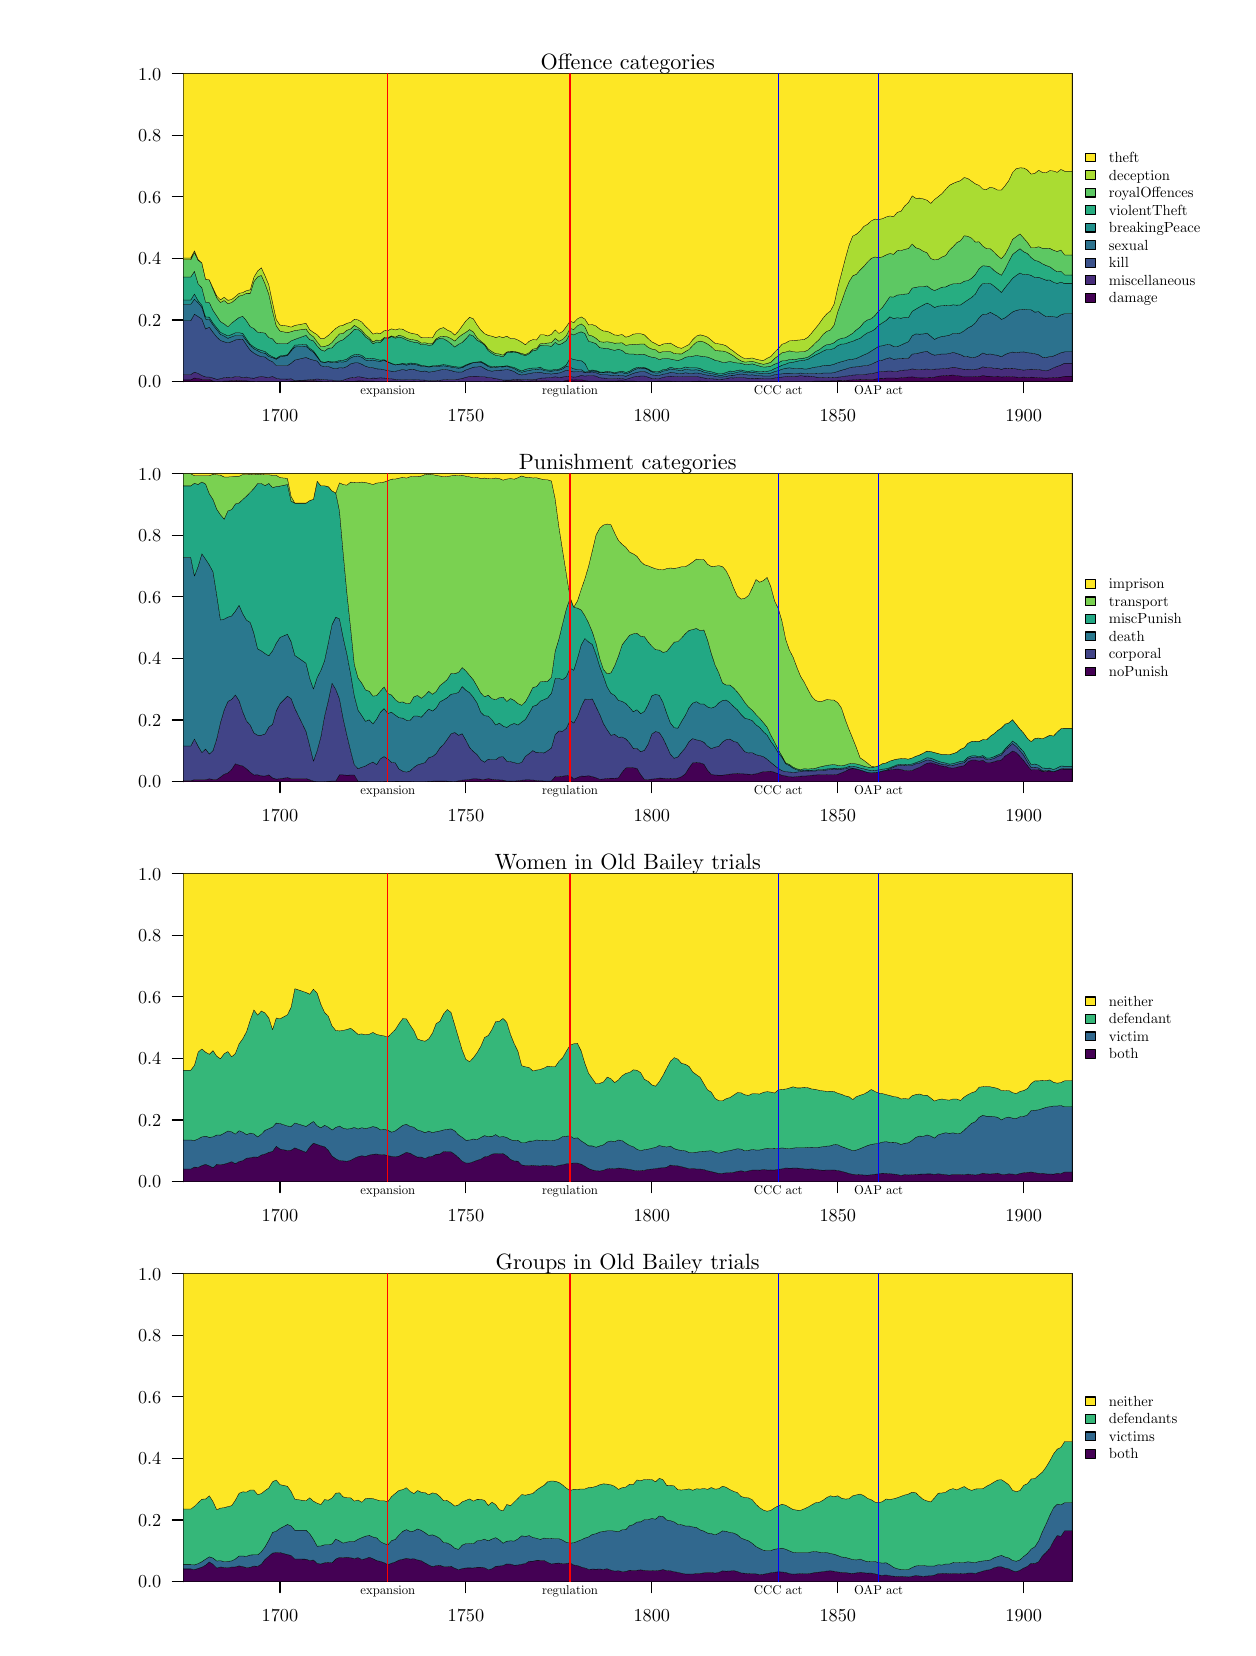
\begin{tikzpicture}[x=1pt,y=1pt]
\definecolor{fillColor}{RGB}{255,255,255}
\path[use as bounding box,fill=fillColor,fill opacity=0.00] (0,0) rectangle (433.62,578.16);
\begin{scope}
\path[clip] (  0.00,  0.00) rectangle (433.62,578.16);
\definecolor{drawColor}{RGB}{0,0,0}

\path[draw=drawColor,line width= 0.4pt,line join=round,line cap=round] ( 91.17,450.25) -- (359.92,450.25);

\path[draw=drawColor,line width= 0.4pt,line join=round,line cap=round] ( 91.17,450.25) -- ( 91.17,446.29);

\path[draw=drawColor,line width= 0.4pt,line join=round,line cap=round] (158.36,450.25) -- (158.36,446.29);

\path[draw=drawColor,line width= 0.4pt,line join=round,line cap=round] (225.54,450.25) -- (225.54,446.29);

\path[draw=drawColor,line width= 0.4pt,line join=round,line cap=round] (292.73,450.25) -- (292.73,446.29);

\path[draw=drawColor,line width= 0.4pt,line join=round,line cap=round] (359.92,450.25) -- (359.92,446.29);

\node[text=drawColor,anchor=base,inner sep=0pt, outer sep=0pt, scale=  0.66] at ( 91.17,436.00) {1700};

\node[text=drawColor,anchor=base,inner sep=0pt, outer sep=0pt, scale=  0.66] at (158.36,436.00) {1750};

\node[text=drawColor,anchor=base,inner sep=0pt, outer sep=0pt, scale=  0.66] at (225.54,436.00) {1800};

\node[text=drawColor,anchor=base,inner sep=0pt, outer sep=0pt, scale=  0.66] at (292.73,436.00) {1850};

\node[text=drawColor,anchor=base,inner sep=0pt, outer sep=0pt, scale=  0.66] at (359.92,436.00) {1900};

\path[draw=drawColor,line width= 0.4pt,line join=round,line cap=round] ( 56.23,450.25) -- ( 56.23,561.53);

\path[draw=drawColor,line width= 0.4pt,line join=round,line cap=round] ( 56.23,450.25) -- ( 52.27,450.25);

\path[draw=drawColor,line width= 0.4pt,line join=round,line cap=round] ( 56.23,472.51) -- ( 52.27,472.51);

\path[draw=drawColor,line width= 0.4pt,line join=round,line cap=round] ( 56.23,494.76) -- ( 52.27,494.76);

\path[draw=drawColor,line width= 0.4pt,line join=round,line cap=round] ( 56.23,517.02) -- ( 52.27,517.02);

\path[draw=drawColor,line width= 0.4pt,line join=round,line cap=round] ( 56.23,539.27) -- ( 52.27,539.27);

\path[draw=drawColor,line width= 0.4pt,line join=round,line cap=round] ( 56.23,561.53) -- ( 52.27,561.53);

\node[text=drawColor,anchor=base east,inner sep=0pt, outer sep=0pt, scale=  0.66] at ( 48.31,447.98) {0.0};

\node[text=drawColor,anchor=base east,inner sep=0pt, outer sep=0pt, scale=  0.66] at ( 48.31,470.23) {0.2};

\node[text=drawColor,anchor=base east,inner sep=0pt, outer sep=0pt, scale=  0.66] at ( 48.31,492.49) {0.4};

\node[text=drawColor,anchor=base east,inner sep=0pt, outer sep=0pt, scale=  0.66] at ( 48.31,514.74) {0.6};

\node[text=drawColor,anchor=base east,inner sep=0pt, outer sep=0pt, scale=  0.66] at ( 48.31,537.00) {0.8};

\node[text=drawColor,anchor=base east,inner sep=0pt, outer sep=0pt, scale=  0.66] at ( 48.31,559.25) {1.0};

\path[draw=drawColor,line width= 0.4pt,line join=round,line cap=round] ( 56.23,450.25) --
	(377.39,450.25) --
	(377.39,561.53) --
	( 56.23,561.53) --
	( 56.23,450.25);
\definecolor{fillColor}{RGB}{68,1,84}

\path[draw=drawColor,line width= 0.1pt,line join=round,line cap=round,fill=fillColor] ( 56.23,450.25) --
	( 57.58,450.25) --
	( 58.92,450.25) --
	( 60.26,450.25) --
	( 61.61,450.25) --
	( 62.95,450.25) --
	( 64.29,450.25) --
	( 65.64,450.25) --
	( 66.98,450.25) --
	( 68.33,450.25) --
	( 69.67,450.25) --
	( 71.01,450.25) --
	( 72.36,450.25) --
	( 73.70,450.25) --
	( 75.04,450.25) --
	( 76.39,450.25) --
	( 77.73,450.25) --
	( 79.08,450.25) --
	( 80.42,450.25) --
	( 81.76,450.25) --
	( 83.11,450.25) --
	( 84.45,450.25) --
	( 85.79,450.25) --
	( 87.14,450.25) --
	( 88.48,450.25) --
	( 89.83,450.25) --
	( 91.17,450.25) --
	( 93.86,450.25) --
	( 95.20,450.25) --
	( 96.54,450.25) --
	(100.58,450.25) --
	(101.92,450.25) --
	(103.26,450.25) --
	(104.61,450.25) --
	(105.95,450.25) --
	(107.29,450.25) --
	(108.64,450.25) --
	(109.98,450.25) --
	(111.33,450.25) --
	(112.67,450.25) --
	(114.01,450.25) --
	(115.36,450.25) --
	(116.70,450.25) --
	(118.04,450.25) --
	(119.39,450.25) --
	(120.73,450.25) --
	(122.08,450.25) --
	(123.42,450.25) --
	(124.76,450.25) --
	(126.11,450.25) --
	(127.45,450.25) --
	(128.79,450.25) --
	(130.14,450.25) --
	(131.48,450.25) --
	(132.83,450.25) --
	(134.17,450.25) --
	(135.51,450.25) --
	(136.86,450.25) --
	(138.20,450.25) --
	(139.54,450.25) --
	(140.89,450.25) --
	(142.23,450.25) --
	(143.58,450.25) --
	(144.92,450.25) --
	(146.26,450.25) --
	(147.61,450.25) --
	(148.95,450.25) --
	(150.29,450.25) --
	(151.64,450.25) --
	(152.98,450.25) --
	(154.33,450.25) --
	(155.67,450.25) --
	(157.01,450.25) --
	(158.36,450.25) --
	(159.70,450.25) --
	(161.04,450.25) --
	(162.39,450.25) --
	(163.73,450.25) --
	(165.08,450.25) --
	(166.42,450.25) --
	(167.76,450.25) --
	(169.11,450.25) --
	(170.45,450.25) --
	(171.79,450.25) --
	(173.14,450.25) --
	(174.48,450.25) --
	(175.83,450.25) --
	(177.17,450.25) --
	(178.51,450.25) --
	(179.86,450.25) --
	(181.20,450.25) --
	(182.54,450.25) --
	(183.89,450.25) --
	(185.23,450.25) --
	(186.58,450.25) --
	(187.92,450.25) --
	(189.26,450.25) --
	(190.61,450.25) --
	(191.95,450.25) --
	(193.29,450.25) --
	(194.64,450.25) --
	(195.98,450.25) --
	(197.33,450.25) --
	(198.67,450.25) --
	(200.01,450.25) --
	(201.36,450.25) --
	(202.70,450.25) --
	(204.04,450.25) --
	(205.39,450.25) --
	(206.73,450.25) --
	(208.08,450.25) --
	(209.42,450.25) --
	(210.76,450.25) --
	(212.11,450.25) --
	(213.45,450.25) --
	(214.79,450.25) --
	(216.14,450.25) --
	(217.48,450.25) --
	(218.83,450.25) --
	(220.17,450.25) --
	(221.51,450.25) --
	(222.86,450.25) --
	(224.20,450.25) --
	(225.54,450.25) --
	(226.89,450.25) --
	(228.23,450.25) --
	(229.58,450.25) --
	(230.92,450.25) --
	(232.26,450.25) --
	(233.61,450.25) --
	(234.95,450.25) --
	(236.29,450.25) --
	(237.64,450.25) --
	(238.98,450.25) --
	(240.33,450.25) --
	(241.67,450.25) --
	(243.01,450.25) --
	(244.36,450.25) --
	(245.70,450.25) --
	(247.04,450.25) --
	(248.39,450.25) --
	(249.73,450.25) --
	(251.08,450.25) --
	(252.42,450.25) --
	(253.76,450.25) --
	(255.11,450.25) --
	(256.45,450.25) --
	(257.79,450.25) --
	(259.14,450.25) --
	(260.48,450.25) --
	(261.83,450.25) --
	(263.17,450.25) --
	(264.51,450.25) --
	(265.86,450.25) --
	(267.20,450.25) --
	(268.54,450.25) --
	(269.89,450.25) --
	(271.23,450.25) --
	(272.58,450.25) --
	(273.92,450.25) --
	(275.26,450.25) --
	(276.61,450.25) --
	(277.95,450.25) --
	(279.29,450.25) --
	(280.64,450.25) --
	(281.98,450.25) --
	(283.33,450.25) --
	(284.67,450.25) --
	(286.01,450.25) --
	(287.36,450.25) --
	(288.70,450.25) --
	(290.04,450.25) --
	(291.39,450.25) --
	(292.73,450.25) --
	(294.08,450.25) --
	(295.42,450.25) --
	(296.76,450.25) --
	(298.11,450.25) --
	(299.45,450.25) --
	(300.79,450.25) --
	(302.14,450.25) --
	(303.48,450.25) --
	(304.83,450.25) --
	(306.17,450.25) --
	(307.51,450.25) --
	(308.86,450.25) --
	(310.20,450.25) --
	(311.54,450.25) --
	(312.89,450.25) --
	(314.23,450.25) --
	(315.58,450.25) --
	(316.92,450.25) --
	(318.26,450.25) --
	(319.61,450.25) --
	(320.95,450.25) --
	(322.29,450.25) --
	(323.64,450.25) --
	(324.98,450.25) --
	(326.33,450.25) --
	(327.67,450.25) --
	(329.01,450.25) --
	(330.36,450.25) --
	(331.70,450.25) --
	(333.04,450.25) --
	(334.39,450.25) --
	(335.73,450.25) --
	(337.08,450.25) --
	(338.42,450.25) --
	(339.76,450.25) --
	(341.11,450.25) --
	(342.45,450.25) --
	(343.79,450.25) --
	(345.14,450.25) --
	(346.48,450.25) --
	(347.83,450.25) --
	(349.17,450.25) --
	(350.51,450.25) --
	(351.86,450.25) --
	(353.20,450.25) --
	(354.54,450.25) --
	(355.89,450.25) --
	(357.23,450.25) --
	(358.58,450.25) --
	(359.92,450.25) --
	(361.26,450.25) --
	(362.61,450.25) --
	(363.95,450.25) --
	(365.29,450.25) --
	(366.64,450.25) --
	(367.98,450.25) --
	(369.33,450.25) --
	(370.67,450.25) --
	(372.01,450.25) --
	(373.36,450.25) --
	(374.70,450.25) --
	(376.04,450.25) --
	(377.39,450.25) --
	(377.39,452.22) --
	(376.04,452.22) --
	(374.70,452.22) --
	(373.36,451.87) --
	(372.01,451.82) --
	(370.67,451.70) --
	(369.33,451.67) --
	(367.98,451.50) --
	(366.64,451.61) --
	(365.29,451.72) --
	(363.95,451.83) --
	(362.61,451.88) --
	(361.26,451.75) --
	(359.92,451.91) --
	(358.58,451.79) --
	(357.23,451.88) --
	(355.89,452.07) --
	(354.54,452.12) --
	(353.20,452.03) --
	(351.86,451.93) --
	(350.51,452.24) --
	(349.17,451.98) --
	(347.83,452.21) --
	(346.48,452.22) --
	(345.14,452.46) --
	(343.79,452.04) --
	(342.45,452.15) --
	(341.11,452.00) --
	(339.76,452.01) --
	(338.42,451.97) --
	(337.08,452.28) --
	(335.73,452.44) --
	(334.39,452.63) --
	(333.04,452.56) --
	(331.70,452.50) --
	(330.36,452.37) --
	(329.01,452.21) --
	(327.67,451.87) --
	(326.33,451.70) --
	(324.98,451.69) --
	(323.64,451.61) --
	(322.29,451.61) --
	(320.95,451.81) --
	(319.61,451.98) --
	(318.26,451.90) --
	(316.92,451.78) --
	(315.58,451.69) --
	(314.23,451.47) --
	(312.89,451.56) --
	(311.54,451.56) --
	(310.20,451.53) --
	(308.86,451.43) --
	(307.51,451.42) --
	(306.17,451.13) --
	(304.83,451.08) --
	(303.48,451.09) --
	(302.14,451.03) --
	(300.79,451.07) --
	(299.45,450.98) --
	(298.11,450.89) --
	(296.76,450.79) --
	(295.42,450.73) --
	(294.08,450.61) --
	(292.73,450.62) --
	(291.39,450.54) --
	(290.04,450.52) --
	(288.70,450.48) --
	(287.36,450.50) --
	(286.01,450.46) --
	(284.67,450.45) --
	(283.33,450.38) --
	(281.98,450.37) --
	(280.64,450.30) --
	(279.29,450.33) --
	(277.95,450.32) --
	(276.61,450.33) --
	(275.26,450.34) --
	(273.92,450.35) --
	(272.58,450.32) --
	(271.23,450.32) --
	(269.89,450.31) --
	(268.54,450.32) --
	(267.20,450.33) --
	(265.86,450.32) --
	(264.51,450.32) --
	(263.17,450.32) --
	(261.83,450.31) --
	(260.48,450.35) --
	(259.14,450.36) --
	(257.79,450.38) --
	(256.45,450.36) --
	(255.11,450.37) --
	(253.76,450.38) --
	(252.42,450.38) --
	(251.08,450.36) --
	(249.73,450.36) --
	(248.39,450.37) --
	(247.04,450.36) --
	(245.70,450.39) --
	(244.36,450.39) --
	(243.01,450.44) --
	(241.67,450.42) --
	(240.33,450.41) --
	(238.98,450.35) --
	(237.64,450.38) --
	(236.29,450.33) --
	(234.95,450.33) --
	(233.61,450.35) --
	(232.26,450.43) --
	(230.92,450.43) --
	(229.58,450.48) --
	(228.23,450.45) --
	(226.89,450.41) --
	(225.54,450.36) --
	(224.20,450.34) --
	(222.86,450.32) --
	(221.51,450.32) --
	(220.17,450.39) --
	(218.83,450.45) --
	(217.48,450.45) --
	(216.14,450.46) --
	(214.79,450.55) --
	(213.45,450.53) --
	(212.11,450.47) --
	(210.76,450.50) --
	(209.42,450.49) --
	(208.08,450.43) --
	(206.73,450.44) --
	(205.39,450.43) --
	(204.04,450.48) --
	(202.70,450.47) --
	(201.36,450.64) --
	(200.01,450.97) --
	(198.67,450.94) --
	(197.33,450.87) --
	(195.98,450.93) --
	(194.64,450.74) --
	(193.29,450.35) --
	(191.95,450.44) --
	(190.61,450.47) --
	(189.26,450.43) --
	(187.92,450.58) --
	(186.58,450.70) --
	(185.23,450.65) --
	(183.89,450.62) --
	(182.54,450.56) --
	(181.20,450.50) --
	(179.86,450.38) --
	(178.51,450.53) --
	(177.17,450.60) --
	(175.83,450.67) --
	(174.48,450.58) --
	(173.14,450.58) --
	(171.79,450.39) --
	(170.45,450.37) --
	(169.11,450.31) --
	(167.76,450.31) --
	(166.42,450.31) --
	(165.08,450.31) --
	(163.73,450.25) --
	(162.39,450.25) --
	(161.04,450.25) --
	(159.70,450.25) --
	(158.36,450.25) --
	(157.01,450.25) --
	(155.67,450.25) --
	(154.33,450.32) --
	(152.98,450.32) --
	(151.64,450.32) --
	(150.29,450.32) --
	(148.95,450.32) --
	(147.61,450.25) --
	(146.26,450.25) --
	(144.92,450.25) --
	(143.58,450.30) --
	(142.23,450.34) --
	(140.89,450.37) --
	(139.54,450.42) --
	(138.20,450.42) --
	(136.86,450.42) --
	(135.51,450.46) --
	(134.17,450.42) --
	(132.83,450.45) --
	(131.48,450.45) --
	(130.14,450.40) --
	(128.79,450.36) --
	(127.45,450.36) --
	(126.11,450.33) --
	(124.76,450.47) --
	(123.42,450.47) --
	(122.08,450.43) --
	(120.73,450.58) --
	(119.39,450.54) --
	(118.04,450.40) --
	(116.70,450.40) --
	(115.36,450.45) --
	(114.01,450.30) --
	(112.67,450.30) --
	(111.33,450.30) --
	(109.98,450.30) --
	(108.64,450.25) --
	(107.29,450.25) --
	(105.95,450.46) --
	(104.61,450.46) --
	(103.26,450.71) --
	(101.92,450.71) --
	(100.58,450.71) --
	( 96.54,450.50) --
	( 95.20,450.50) --
	( 93.86,450.25) --
	( 91.17,450.25) --
	( 89.83,450.25) --
	( 88.48,450.25) --
	( 87.14,450.25) --
	( 85.79,450.25) --
	( 84.45,450.25) --
	( 83.11,450.25) --
	( 81.76,450.33) --
	( 80.42,450.39) --
	( 79.08,450.54) --
	( 77.73,450.54) --
	( 76.39,450.75) --
	( 75.04,450.68) --
	( 73.70,450.61) --
	( 72.36,450.46) --
	( 71.01,450.46) --
	( 69.67,450.25) --
	( 68.33,450.25) --
	( 66.98,450.43) --
	( 65.64,451.11) --
	( 64.29,451.11) --
	( 62.95,451.11) --
	( 61.61,451.36) --
	( 60.26,451.56) --
	( 58.92,450.89) --
	( 57.58,450.89) --
	( 56.23,450.89) --
	cycle;
\definecolor{fillColor}{RGB}{71,45,123}

\path[draw=drawColor,line width= 0.1pt,line join=round,line cap=round,fill=fillColor] ( 56.23,450.89) --
	( 57.58,450.89) --
	( 58.92,450.89) --
	( 60.26,451.56) --
	( 61.61,451.36) --
	( 62.95,451.11) --
	( 64.29,451.11) --
	( 65.64,451.11) --
	( 66.98,450.43) --
	( 68.33,450.25) --
	( 69.67,450.25) --
	( 71.01,450.46) --
	( 72.36,450.46) --
	( 73.70,450.61) --
	( 75.04,450.68) --
	( 76.39,450.75) --
	( 77.73,450.54) --
	( 79.08,450.54) --
	( 80.42,450.39) --
	( 81.76,450.33) --
	( 83.11,450.25) --
	( 84.45,450.25) --
	( 85.79,450.25) --
	( 87.14,450.25) --
	( 88.48,450.25) --
	( 89.83,450.25) --
	( 91.17,450.25) --
	( 93.86,450.25) --
	( 95.20,450.50) --
	( 96.54,450.50) --
	(100.58,450.71) --
	(101.92,450.71) --
	(103.26,450.71) --
	(104.61,450.46) --
	(105.95,450.46) --
	(107.29,450.25) --
	(108.64,450.25) --
	(109.98,450.30) --
	(111.33,450.30) --
	(112.67,450.30) --
	(114.01,450.30) --
	(115.36,450.45) --
	(116.70,450.40) --
	(118.04,450.40) --
	(119.39,450.54) --
	(120.73,450.58) --
	(122.08,450.43) --
	(123.42,450.47) --
	(124.76,450.47) --
	(126.11,450.33) --
	(127.45,450.36) --
	(128.79,450.36) --
	(130.14,450.40) --
	(131.48,450.45) --
	(132.83,450.45) --
	(134.17,450.42) --
	(135.51,450.46) --
	(136.86,450.42) --
	(138.20,450.42) --
	(139.54,450.42) --
	(140.89,450.37) --
	(142.23,450.34) --
	(143.58,450.30) --
	(144.92,450.25) --
	(146.26,450.25) --
	(147.61,450.25) --
	(148.95,450.32) --
	(150.29,450.32) --
	(151.64,450.32) --
	(152.98,450.32) --
	(154.33,450.32) --
	(155.67,450.25) --
	(157.01,450.25) --
	(158.36,450.25) --
	(159.70,450.25) --
	(161.04,450.25) --
	(162.39,450.25) --
	(163.73,450.25) --
	(165.08,450.31) --
	(166.42,450.31) --
	(167.76,450.31) --
	(169.11,450.31) --
	(170.45,450.37) --
	(171.79,450.39) --
	(173.14,450.58) --
	(174.48,450.58) --
	(175.83,450.67) --
	(177.17,450.60) --
	(178.51,450.53) --
	(179.86,450.38) --
	(181.20,450.50) --
	(182.54,450.56) --
	(183.89,450.62) --
	(185.23,450.65) --
	(186.58,450.70) --
	(187.92,450.58) --
	(189.26,450.43) --
	(190.61,450.47) --
	(191.95,450.44) --
	(193.29,450.35) --
	(194.64,450.74) --
	(195.98,450.93) --
	(197.33,450.87) --
	(198.67,450.94) --
	(200.01,450.97) --
	(201.36,450.64) --
	(202.70,450.47) --
	(204.04,450.48) --
	(205.39,450.43) --
	(206.73,450.44) --
	(208.08,450.43) --
	(209.42,450.49) --
	(210.76,450.50) --
	(212.11,450.47) --
	(213.45,450.53) --
	(214.79,450.55) --
	(216.14,450.46) --
	(217.48,450.45) --
	(218.83,450.45) --
	(220.17,450.39) --
	(221.51,450.32) --
	(222.86,450.32) --
	(224.20,450.34) --
	(225.54,450.36) --
	(226.89,450.41) --
	(228.23,450.45) --
	(229.58,450.48) --
	(230.92,450.43) --
	(232.26,450.43) --
	(233.61,450.35) --
	(234.95,450.33) --
	(236.29,450.33) --
	(237.64,450.38) --
	(238.98,450.35) --
	(240.33,450.41) --
	(241.67,450.42) --
	(243.01,450.44) --
	(244.36,450.39) --
	(245.70,450.39) --
	(247.04,450.36) --
	(248.39,450.37) --
	(249.73,450.36) --
	(251.08,450.36) --
	(252.42,450.38) --
	(253.76,450.38) --
	(255.11,450.37) --
	(256.45,450.36) --
	(257.79,450.38) --
	(259.14,450.36) --
	(260.48,450.35) --
	(261.83,450.31) --
	(263.17,450.32) --
	(264.51,450.32) --
	(265.86,450.32) --
	(267.20,450.33) --
	(268.54,450.32) --
	(269.89,450.31) --
	(271.23,450.32) --
	(272.58,450.32) --
	(273.92,450.35) --
	(275.26,450.34) --
	(276.61,450.33) --
	(277.95,450.32) --
	(279.29,450.33) --
	(280.64,450.30) --
	(281.98,450.37) --
	(283.33,450.38) --
	(284.67,450.45) --
	(286.01,450.46) --
	(287.36,450.50) --
	(288.70,450.48) --
	(290.04,450.52) --
	(291.39,450.54) --
	(292.73,450.62) --
	(294.08,450.61) --
	(295.42,450.73) --
	(296.76,450.79) --
	(298.11,450.89) --
	(299.45,450.98) --
	(300.79,451.07) --
	(302.14,451.03) --
	(303.48,451.09) --
	(304.83,451.08) --
	(306.17,451.13) --
	(307.51,451.42) --
	(308.86,451.43) --
	(310.20,451.53) --
	(311.54,451.56) --
	(312.89,451.56) --
	(314.23,451.47) --
	(315.58,451.69) --
	(316.92,451.78) --
	(318.26,451.90) --
	(319.61,451.98) --
	(320.95,451.81) --
	(322.29,451.61) --
	(323.64,451.61) --
	(324.98,451.69) --
	(326.33,451.70) --
	(327.67,451.87) --
	(329.01,452.21) --
	(330.36,452.37) --
	(331.70,452.50) --
	(333.04,452.56) --
	(334.39,452.63) --
	(335.73,452.44) --
	(337.08,452.28) --
	(338.42,451.97) --
	(339.76,452.01) --
	(341.11,452.00) --
	(342.45,452.15) --
	(343.79,452.04) --
	(345.14,452.46) --
	(346.48,452.22) --
	(347.83,452.21) --
	(349.17,451.98) --
	(350.51,452.24) --
	(351.86,451.93) --
	(353.20,452.03) --
	(354.54,452.12) --
	(355.89,452.07) --
	(357.23,451.88) --
	(358.58,451.79) --
	(359.92,451.91) --
	(361.26,451.75) --
	(362.61,451.88) --
	(363.95,451.83) --
	(365.29,451.72) --
	(366.64,451.61) --
	(367.98,451.50) --
	(369.33,451.67) --
	(370.67,451.70) --
	(372.01,451.82) --
	(373.36,451.87) --
	(374.70,452.22) --
	(376.04,452.22) --
	(377.39,452.22) --
	(377.39,456.91) --
	(376.04,456.91) --
	(374.70,456.91) --
	(373.36,456.24) --
	(372.01,455.76) --
	(370.67,455.25) --
	(369.33,454.55) --
	(367.98,454.13) --
	(366.64,454.37) --
	(365.29,454.63) --
	(363.95,454.57) --
	(362.61,454.77) --
	(361.26,454.60) --
	(359.92,454.40) --
	(358.58,454.64) --
	(357.23,454.84) --
	(355.89,455.04) --
	(354.54,455.03) --
	(353.20,455.13) --
	(351.86,454.65) --
	(350.51,455.13) --
	(349.17,455.05) --
	(347.83,455.39) --
	(346.48,455.31) --
	(345.14,455.63) --
	(343.79,454.92) --
	(342.45,454.73) --
	(341.11,454.53) --
	(339.76,454.77) --
	(338.42,454.67) --
	(337.08,454.97) --
	(335.73,455.25) --
	(334.39,455.48) --
	(333.04,455.15) --
	(331.70,455.00) --
	(330.36,454.93) --
	(329.01,454.81) --
	(327.67,454.76) --
	(326.33,454.60) --
	(324.98,454.81) --
	(323.64,454.72) --
	(322.29,454.63) --
	(320.95,454.64) --
	(319.61,454.87) --
	(318.26,454.50) --
	(316.92,454.43) --
	(315.58,454.33) --
	(314.23,453.96) --
	(312.89,453.99) --
	(311.54,454.10) --
	(310.20,454.03) --
	(308.86,453.88) --
	(307.51,453.79) --
	(306.17,453.41) --
	(304.83,453.16) --
	(303.48,453.02) --
	(302.14,452.77) --
	(300.79,452.75) --
	(299.45,452.71) --
	(298.11,452.62) --
	(296.76,452.36) --
	(295.42,452.24) --
	(294.08,452.00) --
	(292.73,451.86) --
	(291.39,451.71) --
	(290.04,451.68) --
	(288.70,451.72) --
	(287.36,451.79) --
	(286.01,451.67) --
	(284.67,451.93) --
	(283.33,452.14) --
	(281.98,452.25) --
	(280.64,452.24) --
	(279.29,452.44) --
	(277.95,452.16) --
	(276.61,452.12) --
	(275.26,452.20) --
	(273.92,452.09) --
	(272.58,451.90) --
	(271.23,451.74) --
	(269.89,451.59) --
	(268.54,451.26) --
	(267.20,451.27) --
	(265.86,451.32) --
	(264.51,451.44) --
	(263.17,451.42) --
	(261.83,451.50) --
	(260.48,451.41) --
	(259.14,451.65) --
	(257.79,451.78) --
	(256.45,451.74) --
	(255.11,451.60) --
	(253.76,451.63) --
	(252.42,451.33) --
	(251.08,451.14) --
	(249.73,451.08) --
	(248.39,451.21) --
	(247.04,451.29) --
	(245.70,451.38) --
	(244.36,451.58) --
	(243.01,451.89) --
	(241.67,452.11) --
	(240.33,452.11) --
	(238.98,452.12) --
	(237.64,452.13) --
	(236.29,452.03) --
	(234.95,452.05) --
	(233.61,452.14) --
	(232.26,452.24) --
	(230.92,452.04) --
	(229.58,451.80) --
	(228.23,451.37) --
	(226.89,451.34) --
	(225.54,451.42) --
	(224.20,451.87) --
	(222.86,452.25) --
	(221.51,452.26) --
	(220.17,452.16) --
	(218.83,451.92) --
	(217.48,451.48) --
	(216.14,451.10) --
	(214.79,451.37) --
	(213.45,451.32) --
	(212.11,451.40) --
	(210.76,451.35) --
	(209.42,451.39) --
	(208.08,451.55) --
	(206.73,451.64) --
	(205.39,452.23) --
	(204.04,452.47) --
	(202.70,452.45) --
	(201.36,452.25) --
	(200.01,452.52) --
	(198.67,452.02) --
	(197.33,451.88) --
	(195.98,452.12) --
	(194.64,452.21) --
	(193.29,451.89) --
	(191.95,451.81) --
	(190.61,452.00) --
	(189.26,451.78) --
	(187.92,451.63) --
	(186.58,451.59) --
	(185.23,451.49) --
	(183.89,451.14) --
	(182.54,451.03) --
	(181.20,451.06) --
	(179.86,450.90) --
	(178.51,451.02) --
	(177.17,451.12) --
	(175.83,451.10) --
	(174.48,450.82) --
	(173.14,450.88) --
	(171.79,450.79) --
	(170.45,451.11) --
	(169.11,451.34) --
	(167.76,451.62) --
	(166.42,451.72) --
	(165.08,452.02) --
	(163.73,452.01) --
	(162.39,452.22) --
	(161.04,452.21) --
	(159.70,452.12) --
	(158.36,451.80) --
	(157.01,451.40) --
	(155.67,451.15) --
	(154.33,451.01) --
	(152.98,451.02) --
	(151.64,450.98) --
	(150.29,450.92) --
	(148.95,450.76) --
	(147.61,450.67) --
	(146.26,450.70) --
	(144.92,450.56) --
	(143.58,450.79) --
	(142.23,450.82) --
	(140.89,450.96) --
	(139.54,450.88) --
	(138.20,450.97) --
	(136.86,450.91) --
	(135.51,450.95) --
	(134.17,450.91) --
	(132.83,451.07) --
	(131.48,451.28) --
	(130.14,451.34) --
	(128.79,451.55) --
	(127.45,451.64) --
	(126.11,451.50) --
	(124.76,451.53) --
	(123.42,451.44) --
	(122.08,451.55) --
	(120.73,451.87) --
	(119.39,452.05) --
	(118.04,451.72) --
	(116.70,451.68) --
	(115.36,451.29) --
	(114.01,450.79) --
	(112.67,450.56) --
	(111.33,450.56) --
	(109.98,450.84) --
	(108.64,450.87) --
	(107.29,450.94) --
	(105.95,451.08) --
	(104.61,451.21) --
	(103.26,451.07) --
	(101.92,450.96) --
	(100.58,450.83) --
	( 96.54,450.63) --
	( 95.20,451.29) --
	( 93.86,451.15) --
	( 91.17,451.21) --
	( 89.83,451.47) --
	( 88.48,452.10) --
	( 87.14,451.80) --
	( 85.79,451.89) --
	( 84.45,452.15) --
	( 83.11,451.89) --
	( 81.76,451.48) --
	( 80.42,451.59) --
	( 79.08,451.91) --
	( 77.73,451.66) --
	( 76.39,452.09) --
	( 75.04,452.08) --
	( 73.70,451.72) --
	( 72.36,451.69) --
	( 71.01,451.72) --
	( 69.67,451.30) --
	( 68.33,451.09) --
	( 66.98,451.55) --
	( 65.64,451.91) --
	( 64.29,451.97) --
	( 62.95,452.46) --
	( 61.61,453.23) --
	( 60.26,453.66) --
	( 58.92,452.81) --
	( 57.58,452.81) --
	( 56.23,452.81) --
	cycle;
\definecolor{fillColor}{RGB}{59,82,139}

\path[draw=drawColor,line width= 0.1pt,line join=round,line cap=round,fill=fillColor] ( 56.23,452.81) --
	( 57.58,452.81) --
	( 58.92,452.81) --
	( 60.26,453.66) --
	( 61.61,453.23) --
	( 62.95,452.46) --
	( 64.29,451.97) --
	( 65.64,451.91) --
	( 66.98,451.55) --
	( 68.33,451.09) --
	( 69.67,451.30) --
	( 71.01,451.72) --
	( 72.36,451.69) --
	( 73.70,451.72) --
	( 75.04,452.08) --
	( 76.39,452.09) --
	( 77.73,451.66) --
	( 79.08,451.91) --
	( 80.42,451.59) --
	( 81.76,451.48) --
	( 83.11,451.89) --
	( 84.45,452.15) --
	( 85.79,451.89) --
	( 87.14,451.80) --
	( 88.48,452.10) --
	( 89.83,451.47) --
	( 91.17,451.21) --
	( 93.86,451.15) --
	( 95.20,451.29) --
	( 96.54,450.63) --
	(100.58,450.83) --
	(101.92,450.96) --
	(103.26,451.07) --
	(104.61,451.21) --
	(105.95,451.08) --
	(107.29,450.94) --
	(108.64,450.87) --
	(109.98,450.84) --
	(111.33,450.56) --
	(112.67,450.56) --
	(114.01,450.79) --
	(115.36,451.29) --
	(116.70,451.68) --
	(118.04,451.72) --
	(119.39,452.05) --
	(120.73,451.87) --
	(122.08,451.55) --
	(123.42,451.44) --
	(124.76,451.53) --
	(126.11,451.50) --
	(127.45,451.64) --
	(128.79,451.55) --
	(130.14,451.34) --
	(131.48,451.28) --
	(132.83,451.07) --
	(134.17,450.91) --
	(135.51,450.95) --
	(136.86,450.91) --
	(138.20,450.97) --
	(139.54,450.88) --
	(140.89,450.96) --
	(142.23,450.82) --
	(143.58,450.79) --
	(144.92,450.56) --
	(146.26,450.70) --
	(147.61,450.67) --
	(148.95,450.76) --
	(150.29,450.92) --
	(151.64,450.98) --
	(152.98,451.02) --
	(154.33,451.01) --
	(155.67,451.15) --
	(157.01,451.40) --
	(158.36,451.80) --
	(159.70,452.12) --
	(161.04,452.21) --
	(162.39,452.22) --
	(163.73,452.01) --
	(165.08,452.02) --
	(166.42,451.72) --
	(167.76,451.62) --
	(169.11,451.34) --
	(170.45,451.11) --
	(171.79,450.79) --
	(173.14,450.88) --
	(174.48,450.82) --
	(175.83,451.10) --
	(177.17,451.12) --
	(178.51,451.02) --
	(179.86,450.90) --
	(181.20,451.06) --
	(182.54,451.03) --
	(183.89,451.14) --
	(185.23,451.49) --
	(186.58,451.59) --
	(187.92,451.63) --
	(189.26,451.78) --
	(190.61,452.00) --
	(191.95,451.81) --
	(193.29,451.89) --
	(194.64,452.21) --
	(195.98,452.12) --
	(197.33,451.88) --
	(198.67,452.02) --
	(200.01,452.52) --
	(201.36,452.25) --
	(202.70,452.45) --
	(204.04,452.47) --
	(205.39,452.23) --
	(206.73,451.64) --
	(208.08,451.55) --
	(209.42,451.39) --
	(210.76,451.35) --
	(212.11,451.40) --
	(213.45,451.32) --
	(214.79,451.37) --
	(216.14,451.10) --
	(217.48,451.48) --
	(218.83,451.92) --
	(220.17,452.16) --
	(221.51,452.26) --
	(222.86,452.25) --
	(224.20,451.87) --
	(225.54,451.42) --
	(226.89,451.34) --
	(228.23,451.37) --
	(229.58,451.80) --
	(230.92,452.04) --
	(232.26,452.24) --
	(233.61,452.14) --
	(234.95,452.05) --
	(236.29,452.03) --
	(237.64,452.13) --
	(238.98,452.12) --
	(240.33,452.11) --
	(241.67,452.11) --
	(243.01,451.89) --
	(244.36,451.58) --
	(245.70,451.38) --
	(247.04,451.29) --
	(248.39,451.21) --
	(249.73,451.08) --
	(251.08,451.14) --
	(252.42,451.33) --
	(253.76,451.63) --
	(255.11,451.60) --
	(256.45,451.74) --
	(257.79,451.78) --
	(259.14,451.65) --
	(260.48,451.41) --
	(261.83,451.50) --
	(263.17,451.42) --
	(264.51,451.44) --
	(265.86,451.32) --
	(267.20,451.27) --
	(268.54,451.26) --
	(269.89,451.59) --
	(271.23,451.74) --
	(272.58,451.90) --
	(273.92,452.09) --
	(275.26,452.20) --
	(276.61,452.12) --
	(277.95,452.16) --
	(279.29,452.44) --
	(280.64,452.24) --
	(281.98,452.25) --
	(283.33,452.14) --
	(284.67,451.93) --
	(286.01,451.67) --
	(287.36,451.79) --
	(288.70,451.72) --
	(290.04,451.68) --
	(291.39,451.71) --
	(292.73,451.86) --
	(294.08,452.00) --
	(295.42,452.24) --
	(296.76,452.36) --
	(298.11,452.62) --
	(299.45,452.71) --
	(300.79,452.75) --
	(302.14,452.77) --
	(303.48,453.02) --
	(304.83,453.16) --
	(306.17,453.41) --
	(307.51,453.79) --
	(308.86,453.88) --
	(310.20,454.03) --
	(311.54,454.10) --
	(312.89,453.99) --
	(314.23,453.96) --
	(315.58,454.33) --
	(316.92,454.43) --
	(318.26,454.50) --
	(319.61,454.87) --
	(320.95,454.64) --
	(322.29,454.63) --
	(323.64,454.72) --
	(324.98,454.81) --
	(326.33,454.60) --
	(327.67,454.76) --
	(329.01,454.81) --
	(330.36,454.93) --
	(331.70,455.00) --
	(333.04,455.15) --
	(334.39,455.48) --
	(335.73,455.25) --
	(337.08,454.97) --
	(338.42,454.67) --
	(339.76,454.77) --
	(341.11,454.53) --
	(342.45,454.73) --
	(343.79,454.92) --
	(345.14,455.63) --
	(346.48,455.31) --
	(347.83,455.39) --
	(349.17,455.05) --
	(350.51,455.13) --
	(351.86,454.65) --
	(353.20,455.13) --
	(354.54,455.03) --
	(355.89,455.04) --
	(357.23,454.84) --
	(358.58,454.64) --
	(359.92,454.40) --
	(361.26,454.60) --
	(362.61,454.77) --
	(363.95,454.57) --
	(365.29,454.63) --
	(366.64,454.37) --
	(367.98,454.13) --
	(369.33,454.55) --
	(370.67,455.25) --
	(372.01,455.76) --
	(373.36,456.24) --
	(374.70,456.91) --
	(376.04,456.91) --
	(377.39,456.91) --
	(377.39,461.01) --
	(376.04,461.01) --
	(374.70,461.01) --
	(373.36,460.68) --
	(372.01,460.10) --
	(370.67,459.49) --
	(369.33,459.32) --
	(367.98,458.97) --
	(366.64,459.09) --
	(365.29,459.97) --
	(363.95,460.33) --
	(362.61,460.57) --
	(361.26,460.70) --
	(359.92,461.01) --
	(358.58,460.92) --
	(357.23,460.76) --
	(355.89,460.94) --
	(354.54,460.58) --
	(353.20,460.08) --
	(351.86,459.20) --
	(350.51,459.79) --
	(349.17,459.94) --
	(347.83,460.27) --
	(346.48,460.10) --
	(345.14,460.64) --
	(343.79,459.64) --
	(342.45,459.10) --
	(341.11,458.92) --
	(339.76,459.28) --
	(338.42,459.34) --
	(337.08,460.02) --
	(335.73,460.43) --
	(334.39,460.85) --
	(333.04,460.40) --
	(331.70,460.22) --
	(330.36,460.27) --
	(329.01,460.02) --
	(327.67,459.81) --
	(326.33,460.33) --
	(324.98,461.19) --
	(323.64,460.98) --
	(322.29,460.65) --
	(320.95,460.35) --
	(319.61,460.22) --
	(318.26,458.69) --
	(316.92,458.67) --
	(315.58,458.64) --
	(314.23,458.48) --
	(312.89,458.33) --
	(311.54,458.89) --
	(310.20,458.52) --
	(308.86,458.01) --
	(307.51,457.77) --
	(306.17,457.16) --
	(304.83,456.53) --
	(303.48,456.09) --
	(302.14,456.01) --
	(300.79,455.78) --
	(299.45,455.60) --
	(298.11,455.52) --
	(296.76,455.21) --
	(295.42,454.73) --
	(294.08,454.38) --
	(292.73,453.94) --
	(291.39,453.51) --
	(290.04,453.34) --
	(288.70,453.37) --
	(287.36,453.33) --
	(286.01,453.12) --
	(284.67,453.15) --
	(283.33,453.21) --
	(281.98,453.15) --
	(280.64,453.08) --
	(279.29,453.37) --
	(277.95,453.14) --
	(276.61,453.12) --
	(275.26,453.31) --
	(273.92,453.30) --
	(272.58,453.07) --
	(271.23,452.95) --
	(269.89,452.76) --
	(268.54,452.33) --
	(267.20,452.25) --
	(265.86,452.31) --
	(264.51,452.38) --
	(263.17,452.51) --
	(261.83,452.72) --
	(260.48,452.62) --
	(259.14,452.89) --
	(257.79,453.04) --
	(256.45,452.85) --
	(255.11,452.52) --
	(253.76,452.50) --
	(252.42,452.13) --
	(251.08,451.93) --
	(249.73,451.95) --
	(248.39,452.19) --
	(247.04,452.47) --
	(245.70,452.60) --
	(244.36,452.81) --
	(243.01,453.25) --
	(241.67,453.40) --
	(240.33,453.28) --
	(238.98,453.27) --
	(237.64,453.46) --
	(236.29,453.10) --
	(234.95,453.22) --
	(233.61,453.46) --
	(232.26,453.62) --
	(230.92,453.12) --
	(229.58,452.96) --
	(228.23,452.55) --
	(226.89,452.49) --
	(225.54,452.71) --
	(224.20,453.36) --
	(222.86,453.94) --
	(221.51,453.91) --
	(220.17,453.62) --
	(218.83,453.26) --
	(217.48,452.69) --
	(216.14,452.19) --
	(214.79,452.49) --
	(213.45,452.51) --
	(212.11,452.48) --
	(210.76,452.56) --
	(209.42,452.73) --
	(208.08,452.70) --
	(206.73,452.91) --
	(205.39,453.47) --
	(204.04,453.75) --
	(202.70,453.62) --
	(201.36,453.50) --
	(200.01,453.95) --
	(198.67,453.85) --
	(197.33,453.77) --
	(195.98,454.17) --
	(194.64,454.38) --
	(193.29,453.80) --
	(191.95,453.35) --
	(190.61,453.28) --
	(189.26,453.00) --
	(187.92,453.16) --
	(186.58,453.28) --
	(185.23,453.68) --
	(183.89,453.55) --
	(182.54,453.42) --
	(181.20,453.18) --
	(179.86,452.90) --
	(178.51,452.66) --
	(177.17,453.03) --
	(175.83,453.87) --
	(174.48,454.39) --
	(173.14,454.65) --
	(171.79,454.42) --
	(170.45,454.40) --
	(169.11,454.28) --
	(167.76,454.02) --
	(166.42,454.31) --
	(165.08,454.99) --
	(163.73,455.79) --
	(162.39,455.55) --
	(161.04,455.48) --
	(159.70,454.94) --
	(158.36,454.51) --
	(157.01,453.74) --
	(155.67,453.69) --
	(154.33,453.84) --
	(152.98,454.29) --
	(151.64,454.53) --
	(150.29,454.65) --
	(148.95,454.45) --
	(147.61,454.12) --
	(146.26,453.88) --
	(144.92,453.67) --
	(143.58,454.09) --
	(142.23,453.93) --
	(140.89,454.23) --
	(139.54,454.67) --
	(138.20,454.76) --
	(136.86,454.33) --
	(135.51,454.65) --
	(134.17,454.31) --
	(132.83,453.99) --
	(131.48,454.02) --
	(130.14,454.22) --
	(128.79,454.55) --
	(127.45,454.83) --
	(126.11,454.87) --
	(124.76,455.28) --
	(123.42,455.39) --
	(122.08,455.82) --
	(120.73,456.53) --
	(119.39,457.07) --
	(118.04,457.03) --
	(116.70,456.67) --
	(115.36,455.71) --
	(114.01,455.19) --
	(112.67,455.30) --
	(111.33,454.89) --
	(109.98,455.19) --
	(108.64,455.75) --
	(107.29,455.59) --
	(105.95,456.03) --
	(104.61,457.69) --
	(103.26,458.04) --
	(101.92,458.42) --
	(100.58,458.99) --
	( 96.54,458.05) --
	( 95.20,456.90) --
	( 93.86,456.07) --
	( 91.17,456.05) --
	( 89.83,456.07) --
	( 88.48,457.43) --
	( 87.14,458.05) --
	( 85.79,459.17) --
	( 84.45,459.26) --
	( 83.11,459.79) --
	( 81.76,460.55) --
	( 80.42,461.62) --
	( 79.08,463.48) --
	( 77.73,465.51) --
	( 76.39,465.61) --
	( 75.04,465.31) --
	( 73.70,464.69) --
	( 72.36,464.26) --
	( 71.01,464.65) --
	( 69.67,465.13) --
	( 68.33,466.37) --
	( 66.98,468.05) --
	( 65.64,469.93) --
	( 64.29,469.29) --
	( 62.95,472.85) --
	( 61.61,473.75) --
	( 60.26,474.62) --
	( 58.92,472.24) --
	( 57.58,472.24) --
	( 56.23,472.24) --
	cycle;
\definecolor{fillColor}{RGB}{44,114,142}

\path[draw=drawColor,line width= 0.1pt,line join=round,line cap=round,fill=fillColor] ( 56.23,472.24) --
	( 57.58,472.24) --
	( 58.92,472.24) --
	( 60.26,474.62) --
	( 61.61,473.75) --
	( 62.95,472.85) --
	( 64.29,469.29) --
	( 65.64,469.93) --
	( 66.98,468.05) --
	( 68.33,466.37) --
	( 69.67,465.13) --
	( 71.01,464.65) --
	( 72.36,464.26) --
	( 73.70,464.69) --
	( 75.04,465.31) --
	( 76.39,465.61) --
	( 77.73,465.51) --
	( 79.08,463.48) --
	( 80.42,461.62) --
	( 81.76,460.55) --
	( 83.11,459.79) --
	( 84.45,459.26) --
	( 85.79,459.17) --
	( 87.14,458.05) --
	( 88.48,457.43) --
	( 89.83,456.07) --
	( 91.17,456.05) --
	( 93.86,456.07) --
	( 95.20,456.90) --
	( 96.54,458.05) --
	(100.58,458.99) --
	(101.92,458.42) --
	(103.26,458.04) --
	(104.61,457.69) --
	(105.95,456.03) --
	(107.29,455.59) --
	(108.64,455.75) --
	(109.98,455.19) --
	(111.33,454.89) --
	(112.67,455.30) --
	(114.01,455.19) --
	(115.36,455.71) --
	(116.70,456.67) --
	(118.04,457.03) --
	(119.39,457.07) --
	(120.73,456.53) --
	(122.08,455.82) --
	(123.42,455.39) --
	(124.76,455.28) --
	(126.11,454.87) --
	(127.45,454.83) --
	(128.79,454.55) --
	(130.14,454.22) --
	(131.48,454.02) --
	(132.83,453.99) --
	(134.17,454.31) --
	(135.51,454.65) --
	(136.86,454.33) --
	(138.20,454.76) --
	(139.54,454.67) --
	(140.89,454.23) --
	(142.23,453.93) --
	(143.58,454.09) --
	(144.92,453.67) --
	(146.26,453.88) --
	(147.61,454.12) --
	(148.95,454.45) --
	(150.29,454.65) --
	(151.64,454.53) --
	(152.98,454.29) --
	(154.33,453.84) --
	(155.67,453.69) --
	(157.01,453.74) --
	(158.36,454.51) --
	(159.70,454.94) --
	(161.04,455.48) --
	(162.39,455.55) --
	(163.73,455.79) --
	(165.08,454.99) --
	(166.42,454.31) --
	(167.76,454.02) --
	(169.11,454.28) --
	(170.45,454.40) --
	(171.79,454.42) --
	(173.14,454.65) --
	(174.48,454.39) --
	(175.83,453.87) --
	(177.17,453.03) --
	(178.51,452.66) --
	(179.86,452.90) --
	(181.20,453.18) --
	(182.54,453.42) --
	(183.89,453.55) --
	(185.23,453.68) --
	(186.58,453.28) --
	(187.92,453.16) --
	(189.26,453.00) --
	(190.61,453.28) --
	(191.95,453.35) --
	(193.29,453.80) --
	(194.64,454.38) --
	(195.98,454.17) --
	(197.33,453.77) --
	(198.67,453.85) --
	(200.01,453.95) --
	(201.36,453.50) --
	(202.70,453.62) --
	(204.04,453.75) --
	(205.39,453.47) --
	(206.73,452.91) --
	(208.08,452.70) --
	(209.42,452.73) --
	(210.76,452.56) --
	(212.11,452.48) --
	(213.45,452.51) --
	(214.79,452.49) --
	(216.14,452.19) --
	(217.48,452.69) --
	(218.83,453.26) --
	(220.17,453.62) --
	(221.51,453.91) --
	(222.86,453.94) --
	(224.20,453.36) --
	(225.54,452.71) --
	(226.89,452.49) --
	(228.23,452.55) --
	(229.58,452.96) --
	(230.92,453.12) --
	(232.26,453.62) --
	(233.61,453.46) --
	(234.95,453.22) --
	(236.29,453.10) --
	(237.64,453.46) --
	(238.98,453.27) --
	(240.33,453.28) --
	(241.67,453.40) --
	(243.01,453.25) --
	(244.36,452.81) --
	(245.70,452.60) --
	(247.04,452.47) --
	(248.39,452.19) --
	(249.73,451.95) --
	(251.08,451.93) --
	(252.42,452.13) --
	(253.76,452.50) --
	(255.11,452.52) --
	(256.45,452.85) --
	(257.79,453.04) --
	(259.14,452.89) --
	(260.48,452.62) --
	(261.83,452.72) --
	(263.17,452.51) --
	(264.51,452.38) --
	(265.86,452.31) --
	(267.20,452.25) --
	(268.54,452.33) --
	(269.89,452.76) --
	(271.23,452.95) --
	(272.58,453.07) --
	(273.92,453.30) --
	(275.26,453.31) --
	(276.61,453.12) --
	(277.95,453.14) --
	(279.29,453.37) --
	(280.64,453.08) --
	(281.98,453.15) --
	(283.33,453.21) --
	(284.67,453.15) --
	(286.01,453.12) --
	(287.36,453.33) --
	(288.70,453.37) --
	(290.04,453.34) --
	(291.39,453.51) --
	(292.73,453.94) --
	(294.08,454.38) --
	(295.42,454.73) --
	(296.76,455.21) --
	(298.11,455.52) --
	(299.45,455.60) --
	(300.79,455.78) --
	(302.14,456.01) --
	(303.48,456.09) --
	(304.83,456.53) --
	(306.17,457.16) --
	(307.51,457.77) --
	(308.86,458.01) --
	(310.20,458.52) --
	(311.54,458.89) --
	(312.89,458.33) --
	(314.23,458.48) --
	(315.58,458.64) --
	(316.92,458.67) --
	(318.26,458.69) --
	(319.61,460.22) --
	(320.95,460.35) --
	(322.29,460.65) --
	(323.64,460.98) --
	(324.98,461.19) --
	(326.33,460.33) --
	(327.67,459.81) --
	(329.01,460.02) --
	(330.36,460.27) --
	(331.70,460.22) --
	(333.04,460.40) --
	(334.39,460.85) --
	(335.73,460.43) --
	(337.08,460.02) --
	(338.42,459.34) --
	(339.76,459.28) --
	(341.11,458.92) --
	(342.45,459.10) --
	(343.79,459.64) --
	(345.14,460.64) --
	(346.48,460.10) --
	(347.83,460.27) --
	(349.17,459.94) --
	(350.51,459.79) --
	(351.86,459.20) --
	(353.20,460.08) --
	(354.54,460.58) --
	(355.89,460.94) --
	(357.23,460.76) --
	(358.58,460.92) --
	(359.92,461.01) --
	(361.26,460.70) --
	(362.61,460.57) --
	(363.95,460.33) --
	(365.29,459.97) --
	(366.64,459.09) --
	(367.98,458.97) --
	(369.33,459.32) --
	(370.67,459.49) --
	(372.01,460.10) --
	(373.36,460.68) --
	(374.70,461.01) --
	(376.04,461.01) --
	(377.39,461.01) --
	(377.39,474.80) --
	(376.04,474.80) --
	(374.70,474.80) --
	(373.36,474.42) --
	(372.01,473.52) --
	(370.67,473.71) --
	(369.33,473.88) --
	(367.98,473.76) --
	(366.64,474.53) --
	(365.29,475.56) --
	(363.95,475.35) --
	(362.61,476.20) --
	(361.26,476.21) --
	(359.92,476.40) --
	(358.58,476.28) --
	(357.23,476.00) --
	(355.89,475.44) --
	(354.54,474.38) --
	(353.20,473.33) --
	(351.86,472.74) --
	(350.51,473.87) --
	(349.17,474.58) --
	(347.83,475.31) --
	(346.48,474.58) --
	(345.14,474.61) --
	(343.79,473.36) --
	(342.45,471.47) --
	(341.11,470.34) --
	(339.76,469.68) --
	(338.42,468.65) --
	(337.08,467.81) --
	(335.73,467.64) --
	(334.39,467.66) --
	(333.04,467.02) --
	(331.70,466.76) --
	(330.36,466.56) --
	(329.01,466.20) --
	(327.67,465.50) --
	(326.33,466.66) --
	(324.98,467.78) --
	(323.64,467.50) --
	(322.29,467.39) --
	(320.95,467.52) --
	(319.61,466.82) --
	(318.26,464.67) --
	(316.92,464.10) --
	(315.58,463.47) --
	(314.23,462.90) --
	(312.89,462.98) --
	(311.54,463.66) --
	(310.20,463.60) --
	(308.86,463.21) --
	(307.51,463.04) --
	(306.17,462.15) --
	(304.83,461.31) --
	(303.48,460.45) --
	(302.14,459.91) --
	(300.79,459.28) --
	(299.45,458.64) --
	(298.11,458.36) --
	(296.76,458.27) --
	(295.42,457.83) --
	(294.08,457.47) --
	(292.73,457.08) --
	(291.39,456.55) --
	(290.04,456.19) --
	(288.70,456.21) --
	(287.36,456.04) --
	(286.01,455.65) --
	(284.67,455.52) --
	(283.33,455.24) --
	(281.98,454.88) --
	(280.64,454.79) --
	(279.29,455.09) --
	(277.95,454.98) --
	(276.61,455.04) --
	(275.26,455.26) --
	(273.92,455.06) --
	(272.58,454.74) --
	(271.23,454.22) --
	(269.89,453.88) --
	(268.54,453.34) --
	(267.20,453.19) --
	(265.86,453.20) --
	(264.51,453.30) --
	(263.17,453.42) --
	(261.83,453.68) --
	(260.48,453.45) --
	(259.14,453.61) --
	(257.79,453.89) --
	(256.45,453.67) --
	(255.11,453.27) --
	(253.76,453.37) --
	(252.42,452.91) --
	(251.08,452.60) --
	(249.73,452.58) --
	(248.39,452.89) --
	(247.04,453.21) --
	(245.70,453.41) --
	(244.36,453.68) --
	(243.01,454.29) --
	(241.67,454.52) --
	(240.33,454.47) --
	(238.98,454.51) --
	(237.64,454.68) --
	(236.29,454.24) --
	(234.95,454.42) --
	(233.61,454.60) --
	(232.26,454.85) --
	(230.92,454.27) --
	(229.58,454.07) --
	(228.23,453.44) --
	(226.89,453.34) --
	(225.54,453.77) --
	(224.20,454.56) --
	(222.86,455.12) --
	(221.51,455.08) --
	(220.17,454.92) --
	(218.83,454.34) --
	(217.48,453.54) --
	(216.14,453.06) --
	(214.79,453.56) --
	(213.45,453.44) --
	(212.11,453.20) --
	(210.76,453.46) --
	(209.42,453.61) --
	(208.08,453.42) --
	(206.73,453.47) --
	(205.39,454.00) --
	(204.04,454.14) --
	(202.70,453.90) --
	(201.36,453.70) --
	(200.01,454.62) --
	(198.67,454.64) --
	(197.33,454.89) --
	(195.98,455.46) --
	(194.64,455.78) --
	(193.29,454.86) --
	(191.95,454.37) --
	(190.61,454.26) --
	(189.26,454.00) --
	(187.92,454.10) --
	(186.58,454.26) --
	(185.23,454.90) --
	(183.89,454.60) --
	(182.54,454.56) --
	(181.20,454.31) --
	(179.86,454.03) --
	(178.51,453.61) --
	(177.17,454.16) --
	(175.83,454.96) --
	(174.48,455.41) --
	(173.14,455.75) --
	(171.79,455.56) --
	(170.45,455.61) --
	(169.11,455.40) --
	(167.76,455.29) --
	(166.42,455.70) --
	(165.08,456.58) --
	(163.73,457.29) --
	(162.39,457.13) --
	(161.04,457.15) --
	(159.70,456.58) --
	(158.36,456.02) --
	(157.01,455.29) --
	(155.67,455.11) --
	(154.33,455.29) --
	(152.98,455.52) --
	(151.64,455.78) --
	(150.29,455.97) --
	(148.95,455.85) --
	(147.61,455.74) --
	(146.26,455.70) --
	(144.92,455.50) --
	(143.58,455.80) --
	(142.23,455.80) --
	(140.89,456.24) --
	(139.54,456.52) --
	(138.20,456.61) --
	(136.86,456.19) --
	(135.51,456.64) --
	(134.17,456.43) --
	(132.83,456.29) --
	(131.48,456.72) --
	(130.14,457.27) --
	(128.79,457.94) --
	(127.45,457.61) --
	(126.11,457.71) --
	(124.76,458.05) --
	(123.42,457.95) --
	(122.08,458.04) --
	(120.73,459.06) --
	(119.39,459.52) --
	(118.04,459.36) --
	(116.70,458.84) --
	(115.36,457.72) --
	(114.01,457.32) --
	(112.67,457.44) --
	(111.33,457.10) --
	(109.98,457.10) --
	(108.64,457.45) --
	(107.29,457.11) --
	(105.95,457.42) --
	(104.61,459.14) --
	(103.26,460.87) --
	(101.92,461.82) --
	(100.58,463.03) --
	( 96.54,462.79) --
	( 95.20,461.32) --
	( 93.86,459.68) --
	( 91.17,459.19) --
	( 89.83,458.33) --
	( 88.48,458.92) --
	( 87.14,459.35) --
	( 85.79,460.50) --
	( 84.45,460.73) --
	( 83.11,461.43) --
	( 81.76,462.14) --
	( 80.42,463.29) --
	( 79.08,465.00) --
	( 77.73,466.88) --
	( 76.39,466.92) --
	( 75.04,466.90) --
	( 73.70,466.45) --
	( 72.36,465.92) --
	( 71.01,466.70) --
	( 69.67,467.33) --
	( 68.33,469.04) --
	( 66.98,470.71) --
	( 65.64,472.75) --
	( 64.29,472.85) --
	( 62.95,477.11) --
	( 61.61,478.73) --
	( 60.26,480.01) --
	( 58.92,478.20) --
	( 57.58,478.20) --
	( 56.23,478.20) --
	cycle;
\definecolor{fillColor}{RGB}{33,144,140}

\path[draw=drawColor,line width= 0.1pt,line join=round,line cap=round,fill=fillColor] ( 56.23,478.20) --
	( 57.58,478.20) --
	( 58.92,478.20) --
	( 60.26,480.01) --
	( 61.61,478.73) --
	( 62.95,477.11) --
	( 64.29,472.85) --
	( 65.64,472.75) --
	( 66.98,470.71) --
	( 68.33,469.04) --
	( 69.67,467.33) --
	( 71.01,466.70) --
	( 72.36,465.92) --
	( 73.70,466.45) --
	( 75.04,466.90) --
	( 76.39,466.92) --
	( 77.73,466.88) --
	( 79.08,465.00) --
	( 80.42,463.29) --
	( 81.76,462.14) --
	( 83.11,461.43) --
	( 84.45,460.73) --
	( 85.79,460.50) --
	( 87.14,459.35) --
	( 88.48,458.92) --
	( 89.83,458.33) --
	( 91.17,459.19) --
	( 93.86,459.68) --
	( 95.20,461.32) --
	( 96.54,462.79) --
	(100.58,463.03) --
	(101.92,461.82) --
	(103.26,460.87) --
	(104.61,459.14) --
	(105.95,457.42) --
	(107.29,457.11) --
	(108.64,457.45) --
	(109.98,457.10) --
	(111.33,457.10) --
	(112.67,457.44) --
	(114.01,457.32) --
	(115.36,457.72) --
	(116.70,458.84) --
	(118.04,459.36) --
	(119.39,459.52) --
	(120.73,459.06) --
	(122.08,458.04) --
	(123.42,457.95) --
	(124.76,458.05) --
	(126.11,457.71) --
	(127.45,457.61) --
	(128.79,457.94) --
	(130.14,457.27) --
	(131.48,456.72) --
	(132.83,456.29) --
	(134.17,456.43) --
	(135.51,456.64) --
	(136.86,456.19) --
	(138.20,456.61) --
	(139.54,456.52) --
	(140.89,456.24) --
	(142.23,455.80) --
	(143.58,455.80) --
	(144.92,455.50) --
	(146.26,455.70) --
	(147.61,455.74) --
	(148.95,455.85) --
	(150.29,455.97) --
	(151.64,455.78) --
	(152.98,455.52) --
	(154.33,455.29) --
	(155.67,455.11) --
	(157.01,455.29) --
	(158.36,456.02) --
	(159.70,456.58) --
	(161.04,457.15) --
	(162.39,457.13) --
	(163.73,457.29) --
	(165.08,456.58) --
	(166.42,455.70) --
	(167.76,455.29) --
	(169.11,455.40) --
	(170.45,455.61) --
	(171.79,455.56) --
	(173.14,455.75) --
	(174.48,455.41) --
	(175.83,454.96) --
	(177.17,454.16) --
	(178.51,453.61) --
	(179.86,454.03) --
	(181.20,454.31) --
	(182.54,454.56) --
	(183.89,454.60) --
	(185.23,454.90) --
	(186.58,454.26) --
	(187.92,454.10) --
	(189.26,454.00) --
	(190.61,454.26) --
	(191.95,454.37) --
	(193.29,454.86) --
	(194.64,455.78) --
	(195.98,455.46) --
	(197.33,454.89) --
	(198.67,454.64) --
	(200.01,454.62) --
	(201.36,453.70) --
	(202.70,453.90) --
	(204.04,454.14) --
	(205.39,454.00) --
	(206.73,453.47) --
	(208.08,453.42) --
	(209.42,453.61) --
	(210.76,453.46) --
	(212.11,453.20) --
	(213.45,453.44) --
	(214.79,453.56) --
	(216.14,453.06) --
	(217.48,453.54) --
	(218.83,454.34) --
	(220.17,454.92) --
	(221.51,455.08) --
	(222.86,455.12) --
	(224.20,454.56) --
	(225.54,453.77) --
	(226.89,453.34) --
	(228.23,453.44) --
	(229.58,454.07) --
	(230.92,454.27) --
	(232.26,454.85) --
	(233.61,454.60) --
	(234.95,454.42) --
	(236.29,454.24) --
	(237.64,454.68) --
	(238.98,454.51) --
	(240.33,454.47) --
	(241.67,454.52) --
	(243.01,454.29) --
	(244.36,453.68) --
	(245.70,453.41) --
	(247.04,453.21) --
	(248.39,452.89) --
	(249.73,452.58) --
	(251.08,452.60) --
	(252.42,452.91) --
	(253.76,453.37) --
	(255.11,453.27) --
	(256.45,453.67) --
	(257.79,453.89) --
	(259.14,453.61) --
	(260.48,453.45) --
	(261.83,453.68) --
	(263.17,453.42) --
	(264.51,453.30) --
	(265.86,453.20) --
	(267.20,453.19) --
	(268.54,453.34) --
	(269.89,453.88) --
	(271.23,454.22) --
	(272.58,454.74) --
	(273.92,455.06) --
	(275.26,455.26) --
	(276.61,455.04) --
	(277.95,454.98) --
	(279.29,455.09) --
	(280.64,454.79) --
	(281.98,454.88) --
	(283.33,455.24) --
	(284.67,455.52) --
	(286.01,455.65) --
	(287.36,456.04) --
	(288.70,456.21) --
	(290.04,456.19) --
	(291.39,456.55) --
	(292.73,457.08) --
	(294.08,457.47) --
	(295.42,457.83) --
	(296.76,458.27) --
	(298.11,458.36) --
	(299.45,458.64) --
	(300.79,459.28) --
	(302.14,459.91) --
	(303.48,460.45) --
	(304.83,461.31) --
	(306.17,462.15) --
	(307.51,463.04) --
	(308.86,463.21) --
	(310.20,463.60) --
	(311.54,463.66) --
	(312.89,462.98) --
	(314.23,462.90) --
	(315.58,463.47) --
	(316.92,464.10) --
	(318.26,464.67) --
	(319.61,466.82) --
	(320.95,467.52) --
	(322.29,467.39) --
	(323.64,467.50) --
	(324.98,467.78) --
	(326.33,466.66) --
	(327.67,465.50) --
	(329.01,466.20) --
	(330.36,466.56) --
	(331.70,466.76) --
	(333.04,467.02) --
	(334.39,467.66) --
	(335.73,467.64) --
	(337.08,467.81) --
	(338.42,468.65) --
	(339.76,469.68) --
	(341.11,470.34) --
	(342.45,471.47) --
	(343.79,473.36) --
	(345.14,474.61) --
	(346.48,474.58) --
	(347.83,475.31) --
	(349.17,474.58) --
	(350.51,473.87) --
	(351.86,472.74) --
	(353.20,473.33) --
	(354.54,474.38) --
	(355.89,475.44) --
	(357.23,476.00) --
	(358.58,476.28) --
	(359.92,476.40) --
	(361.26,476.21) --
	(362.61,476.20) --
	(363.95,475.35) --
	(365.29,475.56) --
	(366.64,474.53) --
	(367.98,473.76) --
	(369.33,473.88) --
	(370.67,473.71) --
	(372.01,473.52) --
	(373.36,474.42) --
	(374.70,474.80) --
	(376.04,474.80) --
	(377.39,474.80) --
	(377.39,485.67) --
	(376.04,485.67) --
	(374.70,485.67) --
	(373.36,486.22) --
	(372.01,485.71) --
	(370.67,486.16) --
	(369.33,486.95) --
	(367.98,486.92) --
	(366.64,487.47) --
	(365.29,487.95) --
	(363.95,487.88) --
	(362.61,488.63) --
	(361.26,489.05) --
	(359.92,488.86) --
	(358.58,489.53) --
	(357.23,488.62) --
	(355.89,487.58) --
	(354.54,485.87) --
	(353.20,484.26) --
	(351.86,482.47) --
	(350.51,483.68) --
	(349.17,484.80) --
	(347.83,485.75) --
	(346.48,485.59) --
	(345.14,485.75) --
	(343.79,484.30) --
	(342.45,481.93) --
	(341.11,480.68) --
	(339.76,479.82) --
	(338.42,478.90) --
	(337.08,477.98) --
	(335.73,477.88) --
	(334.39,478.02) --
	(333.04,477.67) --
	(331.70,477.73) --
	(330.36,477.69) --
	(329.01,477.53) --
	(327.67,477.04) --
	(326.33,478.02) --
	(324.98,478.66) --
	(323.64,477.95) --
	(322.29,477.26) --
	(320.95,476.45) --
	(319.61,475.66) --
	(318.26,473.41) --
	(316.92,473.50) --
	(315.58,473.16) --
	(314.23,473.35) --
	(312.89,473.06) --
	(311.54,473.67) --
	(310.20,472.35) --
	(308.86,471.50) --
	(307.51,470.63) --
	(306.17,469.22) --
	(304.83,468.39) --
	(303.48,467.91) --
	(302.14,467.02) --
	(300.79,465.92) --
	(299.45,465.44) --
	(298.11,464.83) --
	(296.76,464.45) --
	(295.42,463.92) --
	(294.08,463.82) --
	(292.73,463.29) --
	(291.39,462.25) --
	(290.04,461.85) --
	(288.70,461.86) --
	(287.36,461.25) --
	(286.01,460.49) --
	(284.67,459.90) --
	(283.33,459.13) --
	(281.98,458.35) --
	(280.64,457.98) --
	(279.29,457.91) --
	(277.95,457.58) --
	(276.61,457.27) --
	(275.26,457.16) --
	(273.92,456.58) --
	(272.58,456.18) --
	(271.23,455.49) --
	(269.89,454.98) --
	(268.54,454.26) --
	(267.20,453.98) --
	(265.86,453.86) --
	(264.51,453.91) --
	(263.17,453.97) --
	(261.83,454.20) --
	(260.48,453.96) --
	(259.14,454.10) --
	(257.79,454.49) --
	(256.45,454.32) --
	(255.11,453.93) --
	(253.76,454.08) --
	(252.42,453.55) --
	(251.08,453.14) --
	(249.73,453.06) --
	(248.39,453.41) --
	(247.04,453.83) --
	(245.70,454.05) --
	(244.36,454.34) --
	(243.01,455.01) --
	(241.67,455.28) --
	(240.33,455.24) --
	(238.98,455.29) --
	(237.64,455.56) --
	(236.29,455.01) --
	(234.95,455.03) --
	(233.61,455.08) --
	(232.26,455.48) --
	(230.92,454.75) --
	(229.58,454.59) --
	(228.23,453.96) --
	(226.89,453.87) --
	(225.54,454.07) --
	(224.20,454.85) --
	(222.86,455.37) --
	(221.51,455.46) --
	(220.17,455.37) --
	(218.83,454.87) --
	(217.48,454.03) --
	(216.14,453.56) --
	(214.79,454.06) --
	(213.45,453.81) --
	(212.11,453.51) --
	(210.76,453.79) --
	(209.42,453.99) --
	(208.08,453.67) --
	(206.73,453.74) --
	(205.39,454.27) --
	(204.04,454.46) --
	(202.70,454.25) --
	(201.36,456.86) --
	(200.01,457.83) --
	(198.67,458.01) --
	(197.33,458.23) --
	(195.98,458.74) --
	(194.64,456.34) --
	(193.29,455.37) --
	(191.95,454.75) --
	(190.61,454.70) --
	(189.26,454.40) --
	(187.92,454.47) --
	(186.58,454.69) --
	(185.23,455.50) --
	(183.89,455.15) --
	(182.54,455.16) --
	(181.20,455.03) --
	(179.86,454.67) --
	(178.51,454.10) --
	(177.17,454.69) --
	(175.83,455.39) --
	(174.48,455.66) --
	(173.14,456.03) --
	(171.79,455.77) --
	(170.45,455.74) --
	(169.11,455.65) --
	(167.76,455.71) --
	(166.42,456.05) --
	(165.08,456.87) --
	(163.73,457.57) --
	(162.39,457.34) --
	(161.04,457.23) --
	(159.70,456.81) --
	(158.36,456.33) --
	(157.01,455.60) --
	(155.67,455.50) --
	(154.33,455.71) --
	(152.98,455.90) --
	(151.64,456.21) --
	(150.29,456.40) --
	(148.95,456.20) --
	(147.61,456.02) --
	(146.26,455.96) --
	(144.92,455.63) --
	(143.58,455.98) --
	(142.23,456.13) --
	(140.89,456.64) --
	(139.54,456.89) --
	(138.20,456.97) --
	(136.86,456.60) --
	(135.51,456.85) --
	(134.17,456.56) --
	(132.83,456.41) --
	(131.48,456.85) --
	(130.14,457.48) --
	(128.79,458.19) --
	(127.45,458.00) --
	(126.11,458.33) --
	(124.76,458.72) --
	(123.42,458.62) --
	(122.08,458.71) --
	(120.73,459.75) --
	(119.39,460.14) --
	(118.04,460.02) --
	(116.70,459.42) --
	(115.36,458.40) --
	(114.01,457.99) --
	(112.67,457.91) --
	(111.33,457.48) --
	(109.98,457.38) --
	(108.64,457.58) --
	(107.29,457.24) --
	(105.95,457.54) --
	(104.61,459.52) --
	(103.26,461.37) --
	(101.92,462.32) --
	(100.58,463.70) --
	( 96.54,463.46) --
	( 95.20,461.73) --
	( 93.86,459.96) --
	( 91.17,459.54) --
	( 89.83,458.65) --
	( 88.48,459.24) --
	( 87.14,459.97) --
	( 85.79,461.13) --
	( 84.45,461.53) --
	( 83.11,461.97) --
	( 81.76,462.75) --
	( 80.42,463.79) --
	( 79.08,465.65) --
	( 77.73,467.68) --
	( 76.39,467.94) --
	( 75.04,467.91) --
	( 73.70,467.26) --
	( 72.36,466.79) --
	( 71.01,467.40) --
	( 69.67,468.07) --
	( 68.33,469.71) --
	( 66.98,471.38) --
	( 65.64,473.55) --
	( 64.29,473.61) --
	( 62.95,477.87) --
	( 61.61,479.48) --
	( 60.26,481.89) --
	( 58.92,479.74) --
	( 57.58,479.74) --
	( 56.23,479.74) --
	cycle;
\definecolor{fillColor}{RGB}{39,173,129}

\path[draw=drawColor,line width= 0.1pt,line join=round,line cap=round,fill=fillColor] ( 56.23,479.74) --
	( 57.58,479.74) --
	( 58.92,479.74) --
	( 60.26,481.89) --
	( 61.61,479.48) --
	( 62.95,477.87) --
	( 64.29,473.61) --
	( 65.64,473.55) --
	( 66.98,471.38) --
	( 68.33,469.71) --
	( 69.67,468.07) --
	( 71.01,467.40) --
	( 72.36,466.79) --
	( 73.70,467.26) --
	( 75.04,467.91) --
	( 76.39,467.94) --
	( 77.73,467.68) --
	( 79.08,465.65) --
	( 80.42,463.79) --
	( 81.76,462.75) --
	( 83.11,461.97) --
	( 84.45,461.53) --
	( 85.79,461.13) --
	( 87.14,459.97) --
	( 88.48,459.24) --
	( 89.83,458.65) --
	( 91.17,459.54) --
	( 93.86,459.96) --
	( 95.20,461.73) --
	( 96.54,463.46) --
	(100.58,463.70) --
	(101.92,462.32) --
	(103.26,461.37) --
	(104.61,459.52) --
	(105.95,457.54) --
	(107.29,457.24) --
	(108.64,457.58) --
	(109.98,457.38) --
	(111.33,457.48) --
	(112.67,457.91) --
	(114.01,457.99) --
	(115.36,458.40) --
	(116.70,459.42) --
	(118.04,460.02) --
	(119.39,460.14) --
	(120.73,459.75) --
	(122.08,458.71) --
	(123.42,458.62) --
	(124.76,458.72) --
	(126.11,458.33) --
	(127.45,458.00) --
	(128.79,458.19) --
	(130.14,457.48) --
	(131.48,456.85) --
	(132.83,456.41) --
	(134.17,456.56) --
	(135.51,456.85) --
	(136.86,456.60) --
	(138.20,456.97) --
	(139.54,456.89) --
	(140.89,456.64) --
	(142.23,456.13) --
	(143.58,455.98) --
	(144.92,455.63) --
	(146.26,455.96) --
	(147.61,456.02) --
	(148.95,456.20) --
	(150.29,456.40) --
	(151.64,456.21) --
	(152.98,455.90) --
	(154.33,455.71) --
	(155.67,455.50) --
	(157.01,455.60) --
	(158.36,456.33) --
	(159.70,456.81) --
	(161.04,457.23) --
	(162.39,457.34) --
	(163.73,457.57) --
	(165.08,456.87) --
	(166.42,456.05) --
	(167.76,455.71) --
	(169.11,455.65) --
	(170.45,455.74) --
	(171.79,455.77) --
	(173.14,456.03) --
	(174.48,455.66) --
	(175.83,455.39) --
	(177.17,454.69) --
	(178.51,454.10) --
	(179.86,454.67) --
	(181.20,455.03) --
	(182.54,455.16) --
	(183.89,455.15) --
	(185.23,455.50) --
	(186.58,454.69) --
	(187.92,454.47) --
	(189.26,454.40) --
	(190.61,454.70) --
	(191.95,454.75) --
	(193.29,455.37) --
	(194.64,456.34) --
	(195.98,458.74) --
	(197.33,458.23) --
	(198.67,458.01) --
	(200.01,457.83) --
	(201.36,456.86) --
	(202.70,454.25) --
	(204.04,454.46) --
	(205.39,454.27) --
	(206.73,453.74) --
	(208.08,453.67) --
	(209.42,453.99) --
	(210.76,453.79) --
	(212.11,453.51) --
	(213.45,453.81) --
	(214.79,454.06) --
	(216.14,453.56) --
	(217.48,454.03) --
	(218.83,454.87) --
	(220.17,455.37) --
	(221.51,455.46) --
	(222.86,455.37) --
	(224.20,454.85) --
	(225.54,454.07) --
	(226.89,453.87) --
	(228.23,453.96) --
	(229.58,454.59) --
	(230.92,454.75) --
	(232.26,455.48) --
	(233.61,455.08) --
	(234.95,455.03) --
	(236.29,455.01) --
	(237.64,455.56) --
	(238.98,455.29) --
	(240.33,455.24) --
	(241.67,455.28) --
	(243.01,455.01) --
	(244.36,454.34) --
	(245.70,454.05) --
	(247.04,453.83) --
	(248.39,453.41) --
	(249.73,453.06) --
	(251.08,453.14) --
	(252.42,453.55) --
	(253.76,454.08) --
	(255.11,453.93) --
	(256.45,454.32) --
	(257.79,454.49) --
	(259.14,454.10) --
	(260.48,453.96) --
	(261.83,454.20) --
	(263.17,453.97) --
	(264.51,453.91) --
	(265.86,453.86) --
	(267.20,453.98) --
	(268.54,454.26) --
	(269.89,454.98) --
	(271.23,455.49) --
	(272.58,456.18) --
	(273.92,456.58) --
	(275.26,457.16) --
	(276.61,457.27) --
	(277.95,457.58) --
	(279.29,457.91) --
	(280.64,457.98) --
	(281.98,458.35) --
	(283.33,459.13) --
	(284.67,459.90) --
	(286.01,460.49) --
	(287.36,461.25) --
	(288.70,461.86) --
	(290.04,461.85) --
	(291.39,462.25) --
	(292.73,463.29) --
	(294.08,463.82) --
	(295.42,463.92) --
	(296.76,464.45) --
	(298.11,464.83) --
	(299.45,465.44) --
	(300.79,465.92) --
	(302.14,467.02) --
	(303.48,467.91) --
	(304.83,468.39) --
	(306.17,469.22) --
	(307.51,470.63) --
	(308.86,471.50) --
	(310.20,472.35) --
	(311.54,473.67) --
	(312.89,473.06) --
	(314.23,473.35) --
	(315.58,473.16) --
	(316.92,473.50) --
	(318.26,473.41) --
	(319.61,475.66) --
	(320.95,476.45) --
	(322.29,477.26) --
	(323.64,477.95) --
	(324.98,478.66) --
	(326.33,478.02) --
	(327.67,477.04) --
	(329.01,477.53) --
	(330.36,477.69) --
	(331.70,477.73) --
	(333.04,477.67) --
	(334.39,478.02) --
	(335.73,477.88) --
	(337.08,477.98) --
	(338.42,478.90) --
	(339.76,479.82) --
	(341.11,480.68) --
	(342.45,481.93) --
	(343.79,484.30) --
	(345.14,485.75) --
	(346.48,485.59) --
	(347.83,485.75) --
	(349.17,484.80) --
	(350.51,483.68) --
	(351.86,482.47) --
	(353.20,484.26) --
	(354.54,485.87) --
	(355.89,487.58) --
	(357.23,488.62) --
	(358.58,489.53) --
	(359.92,488.86) --
	(361.26,489.05) --
	(362.61,488.63) --
	(363.95,487.88) --
	(365.29,487.95) --
	(366.64,487.47) --
	(367.98,486.92) --
	(369.33,486.95) --
	(370.67,486.16) --
	(372.01,485.71) --
	(373.36,486.22) --
	(374.70,485.67) --
	(376.04,485.67) --
	(377.39,485.67) --
	(377.39,488.81) --
	(376.04,488.81) --
	(374.70,488.81) --
	(373.36,490.15) --
	(372.01,489.92) --
	(370.67,490.79) --
	(369.33,491.79) --
	(367.98,492.22) --
	(366.64,492.86) --
	(365.29,493.71) --
	(363.95,494.08) --
	(362.61,495.08) --
	(361.26,496.55) --
	(359.92,497.17) --
	(358.58,498.29) --
	(357.23,497.26) --
	(355.89,496.22) --
	(354.54,493.68) --
	(353.20,490.97) --
	(351.86,488.71) --
	(350.51,489.49) --
	(349.17,490.46) --
	(347.83,491.75) --
	(346.48,492.02) --
	(345.14,492.13) --
	(343.79,491.07) --
	(342.45,488.98) --
	(341.11,487.61) --
	(339.76,486.79) --
	(338.42,486.54) --
	(337.08,485.75) --
	(335.73,485.63) --
	(334.39,485.59) --
	(333.04,485.15) --
	(331.70,484.48) --
	(330.36,484.38) --
	(329.01,483.74) --
	(327.67,483.16) --
	(326.33,483.80) --
	(324.98,484.87) --
	(323.64,484.51) --
	(322.29,484.57) --
	(320.95,484.34) --
	(319.61,484.06) --
	(318.26,482.01) --
	(316.92,481.88) --
	(315.58,481.65) --
	(314.23,481.56) --
	(312.89,480.81) --
	(311.54,480.92) --
	(310.20,478.98) --
	(308.86,477.07) --
	(307.51,475.77) --
	(306.17,474.16) --
	(304.83,472.99) --
	(303.48,472.56) --
	(302.14,471.65) --
	(300.79,469.93) --
	(299.45,468.97) --
	(298.11,467.72) --
	(296.76,466.88) --
	(295.42,466.10) --
	(294.08,465.93) --
	(292.73,465.39) --
	(291.39,464.30) --
	(290.04,463.78) --
	(288.70,463.60) --
	(287.36,462.84) --
	(286.01,461.76) --
	(284.67,461.11) --
	(283.33,460.04) --
	(281.98,459.14) --
	(280.64,458.75) --
	(279.29,458.72) --
	(277.95,458.38) --
	(276.61,458.30) --
	(275.26,458.25) --
	(273.92,457.82) --
	(272.58,457.76) --
	(271.23,457.08) --
	(269.89,456.55) --
	(268.54,455.85) --
	(267.20,455.60) --
	(265.86,455.53) --
	(264.51,455.88) --
	(263.17,456.26) --
	(261.83,456.69) --
	(260.48,456.47) --
	(259.14,456.45) --
	(257.79,456.92) --
	(256.45,456.99) --
	(255.11,457.23) --
	(253.76,457.55) --
	(252.42,457.27) --
	(251.08,457.22) --
	(249.73,457.70) --
	(248.39,457.97) --
	(247.04,458.62) --
	(245.70,459.13) --
	(244.36,459.32) --
	(243.01,459.48) --
	(241.67,459.73) --
	(240.33,459.43) --
	(238.98,459.30) --
	(237.64,459.07) --
	(236.29,458.27) --
	(234.95,457.90) --
	(233.61,458.14) --
	(232.26,458.43) --
	(230.92,458.64) --
	(229.58,458.60) --
	(228.23,458.22) --
	(226.89,458.88) --
	(225.54,459.09) --
	(224.20,459.47) --
	(222.86,460.09) --
	(221.51,460.16) --
	(220.17,459.91) --
	(218.83,460.27) --
	(217.48,460.21) --
	(216.14,460.47) --
	(214.79,461.53) --
	(213.45,461.94) --
	(212.11,461.56) --
	(210.76,461.86) --
	(209.42,462.29) --
	(208.08,462.34) --
	(206.73,462.51) --
	(205.39,463.96) --
	(204.04,464.49) --
	(202.70,464.82) --
	(201.36,467.66) --
	(200.01,468.25) --
	(198.67,467.79) --
	(197.33,467.14) --
	(195.98,467.65) --
	(194.64,465.07) --
	(193.29,464.14) --
	(191.95,463.53) --
	(190.61,464.46) --
	(189.26,463.02) --
	(187.92,463.22) --
	(186.58,463.21) --
	(185.23,463.41) --
	(183.89,461.68) --
	(182.54,461.47) --
	(181.20,460.32) --
	(179.86,459.68) --
	(178.51,460.05) --
	(177.17,460.66) --
	(175.83,460.94) --
	(174.48,460.89) --
	(173.14,460.72) --
	(171.79,459.26) --
	(170.45,459.56) --
	(169.11,459.76) --
	(167.76,460.51) --
	(166.42,461.46) --
	(165.08,463.48) --
	(163.73,464.48) --
	(162.39,465.21) --
	(161.04,466.77) --
	(159.70,467.27) --
	(158.36,465.74) --
	(157.01,464.39) --
	(155.67,463.74) --
	(154.33,462.73) --
	(152.98,463.96) --
	(151.64,464.99) --
	(150.29,465.72) --
	(148.95,465.89) --
	(147.61,465.33) --
	(146.26,463.56) --
	(144.92,463.37) --
	(143.58,463.70) --
	(142.23,463.56) --
	(140.89,464.42) --
	(139.54,464.52) --
	(138.20,464.84) --
	(136.86,465.34) --
	(135.51,466.01) --
	(134.17,466.37) --
	(132.83,465.96) --
	(131.48,466.56) --
	(130.14,465.81) --
	(128.79,465.82) --
	(127.45,464.49) --
	(126.11,464.57) --
	(124.76,463.94) --
	(123.42,465.51) --
	(122.08,466.39) --
	(120.73,468.11) --
	(119.39,469.08) --
	(118.04,469.16) --
	(116.70,467.71) --
	(115.36,466.58) --
	(114.01,465.39) --
	(112.67,464.89) --
	(111.33,463.99) --
	(109.98,462.45) --
	(108.64,462.31) --
	(107.29,461.27) --
	(105.95,461.75) --
	(104.61,463.16) --
	(103.26,465.01) --
	(101.92,465.41) --
	(100.58,466.99) --
	( 96.54,465.52) --
	( 95.20,464.99) --
	( 93.86,463.98) --
	( 91.17,463.94) --
	( 89.83,464.13) --
	( 88.48,465.72) --
	( 87.14,466.16) --
	( 85.79,467.76) --
	( 84.45,468.03) --
	( 83.11,468.11) --
	( 81.76,469.43) --
	( 80.42,470.12) --
	( 79.08,472.23) --
	( 77.73,473.83) --
	( 76.39,473.44) --
	( 75.04,472.42) --
	( 73.70,471.39) --
	( 72.36,470.05) --
	( 71.01,471.12) --
	( 69.67,471.91) --
	( 68.33,473.99) --
	( 66.98,475.99) --
	( 65.64,478.85) --
	( 64.29,478.96) --
	( 62.95,484.16) --
	( 61.61,485.56) --
	( 60.26,490.11) --
	( 58.92,488.06) --
	( 57.58,488.06) --
	( 56.23,488.06) --
	cycle;
\definecolor{fillColor}{RGB}{93,200,99}

\path[draw=drawColor,line width= 0.1pt,line join=round,line cap=round,fill=fillColor] ( 56.23,488.06) --
	( 57.58,488.06) --
	( 58.92,488.06) --
	( 60.26,490.11) --
	( 61.61,485.56) --
	( 62.95,484.16) --
	( 64.29,478.96) --
	( 65.64,478.85) --
	( 66.98,475.99) --
	( 68.33,473.99) --
	( 69.67,471.91) --
	( 71.01,471.12) --
	( 72.36,470.05) --
	( 73.70,471.39) --
	( 75.04,472.42) --
	( 76.39,473.44) --
	( 77.73,473.83) --
	( 79.08,472.23) --
	( 80.42,470.12) --
	( 81.76,469.43) --
	( 83.11,468.11) --
	( 84.45,468.03) --
	( 85.79,467.76) --
	( 87.14,466.16) --
	( 88.48,465.72) --
	( 89.83,464.13) --
	( 91.17,463.94) --
	( 93.86,463.98) --
	( 95.20,464.99) --
	( 96.54,465.52) --
	(100.58,466.99) --
	(101.92,465.41) --
	(103.26,465.01) --
	(104.61,463.16) --
	(105.95,461.75) --
	(107.29,461.27) --
	(108.64,462.31) --
	(109.98,462.45) --
	(111.33,463.99) --
	(112.67,464.89) --
	(114.01,465.39) --
	(115.36,466.58) --
	(116.70,467.71) --
	(118.04,469.16) --
	(119.39,469.08) --
	(120.73,468.11) --
	(122.08,466.39) --
	(123.42,465.51) --
	(124.76,463.94) --
	(126.11,464.57) --
	(127.45,464.49) --
	(128.79,465.82) --
	(130.14,465.81) --
	(131.48,466.56) --
	(132.83,465.96) --
	(134.17,466.37) --
	(135.51,466.01) --
	(136.86,465.34) --
	(138.20,464.84) --
	(139.54,464.52) --
	(140.89,464.42) --
	(142.23,463.56) --
	(143.58,463.70) --
	(144.92,463.37) --
	(146.26,463.56) --
	(147.61,465.33) --
	(148.95,465.89) --
	(150.29,465.72) --
	(151.64,464.99) --
	(152.98,463.96) --
	(154.33,462.73) --
	(155.67,463.74) --
	(157.01,464.39) --
	(158.36,465.74) --
	(159.70,467.27) --
	(161.04,466.77) --
	(162.39,465.21) --
	(163.73,464.48) --
	(165.08,463.48) --
	(166.42,461.46) --
	(167.76,460.51) --
	(169.11,459.76) --
	(170.45,459.56) --
	(171.79,459.26) --
	(173.14,460.72) --
	(174.48,460.89) --
	(175.83,460.94) --
	(177.17,460.66) --
	(178.51,460.05) --
	(179.86,459.68) --
	(181.20,460.32) --
	(182.54,461.47) --
	(183.89,461.68) --
	(185.23,463.41) --
	(186.58,463.21) --
	(187.92,463.22) --
	(189.26,463.02) --
	(190.61,464.46) --
	(191.95,463.53) --
	(193.29,464.14) --
	(194.64,465.07) --
	(195.98,467.65) --
	(197.33,467.14) --
	(198.67,467.79) --
	(200.01,468.25) --
	(201.36,467.66) --
	(202.70,464.82) --
	(204.04,464.49) --
	(205.39,463.96) --
	(206.73,462.51) --
	(208.08,462.34) --
	(209.42,462.29) --
	(210.76,461.86) --
	(212.11,461.56) --
	(213.45,461.94) --
	(214.79,461.53) --
	(216.14,460.47) --
	(217.48,460.21) --
	(218.83,460.27) --
	(220.17,459.91) --
	(221.51,460.16) --
	(222.86,460.09) --
	(224.20,459.47) --
	(225.54,459.09) --
	(226.89,458.88) --
	(228.23,458.22) --
	(229.58,458.60) --
	(230.92,458.64) --
	(232.26,458.43) --
	(233.61,458.14) --
	(234.95,457.90) --
	(236.29,458.27) --
	(237.64,459.07) --
	(238.98,459.30) --
	(240.33,459.43) --
	(241.67,459.73) --
	(243.01,459.48) --
	(244.36,459.32) --
	(245.70,459.13) --
	(247.04,458.62) --
	(248.39,457.97) --
	(249.73,457.70) --
	(251.08,457.22) --
	(252.42,457.27) --
	(253.76,457.55) --
	(255.11,457.23) --
	(256.45,456.99) --
	(257.79,456.92) --
	(259.14,456.45) --
	(260.48,456.47) --
	(261.83,456.69) --
	(263.17,456.26) --
	(264.51,455.88) --
	(265.86,455.53) --
	(267.20,455.60) --
	(268.54,455.85) --
	(269.89,456.55) --
	(271.23,457.08) --
	(272.58,457.76) --
	(273.92,457.82) --
	(275.26,458.25) --
	(276.61,458.30) --
	(277.95,458.38) --
	(279.29,458.72) --
	(280.64,458.75) --
	(281.98,459.14) --
	(283.33,460.04) --
	(284.67,461.11) --
	(286.01,461.76) --
	(287.36,462.84) --
	(288.70,463.60) --
	(290.04,463.78) --
	(291.39,464.30) --
	(292.73,465.39) --
	(294.08,465.93) --
	(295.42,466.10) --
	(296.76,466.88) --
	(298.11,467.72) --
	(299.45,468.97) --
	(300.79,469.93) --
	(302.14,471.65) --
	(303.48,472.56) --
	(304.83,472.99) --
	(306.17,474.16) --
	(307.51,475.77) --
	(308.86,477.07) --
	(310.20,478.98) --
	(311.54,480.92) --
	(312.89,480.81) --
	(314.23,481.56) --
	(315.58,481.65) --
	(316.92,481.88) --
	(318.26,482.01) --
	(319.61,484.06) --
	(320.95,484.34) --
	(322.29,484.57) --
	(323.64,484.51) --
	(324.98,484.87) --
	(326.33,483.80) --
	(327.67,483.16) --
	(329.01,483.74) --
	(330.36,484.38) --
	(331.70,484.48) --
	(333.04,485.15) --
	(334.39,485.59) --
	(335.73,485.63) --
	(337.08,485.75) --
	(338.42,486.54) --
	(339.76,486.79) --
	(341.11,487.61) --
	(342.45,488.98) --
	(343.79,491.07) --
	(345.14,492.13) --
	(346.48,492.02) --
	(347.83,491.75) --
	(349.17,490.46) --
	(350.51,489.49) --
	(351.86,488.71) --
	(353.20,490.97) --
	(354.54,493.68) --
	(355.89,496.22) --
	(357.23,497.26) --
	(358.58,498.29) --
	(359.92,497.17) --
	(361.26,496.55) --
	(362.61,495.08) --
	(363.95,494.08) --
	(365.29,493.71) --
	(366.64,492.86) --
	(367.98,492.22) --
	(369.33,491.79) --
	(370.67,490.79) --
	(372.01,489.92) --
	(373.36,490.15) --
	(374.70,488.81) --
	(376.04,488.81) --
	(377.39,488.81) --
	(377.39,496.03) --
	(376.04,496.03) --
	(374.70,496.03) --
	(373.36,497.82) --
	(372.01,497.28) --
	(370.67,497.74) --
	(369.33,498.40) --
	(367.98,498.48) --
	(366.64,498.45) --
	(365.29,499.01) --
	(363.95,498.60) --
	(362.61,498.60) --
	(361.26,500.60) --
	(359.92,502.11) --
	(358.58,503.64) --
	(357.23,502.66) --
	(355.89,501.66) --
	(354.54,498.80) --
	(353.20,496.29) --
	(351.86,494.69) --
	(350.51,495.71) --
	(349.17,497.10) --
	(347.83,498.28) --
	(346.48,498.30) --
	(345.14,499.22) --
	(343.79,500.77) --
	(342.45,500.72) --
	(341.11,502.09) --
	(339.76,502.78) --
	(338.42,502.97) --
	(337.08,501.16) --
	(335.73,500.48) --
	(334.39,499.02) --
	(333.04,497.76) --
	(331.70,495.82) --
	(330.36,495.28) --
	(329.01,494.44) --
	(327.67,494.25) --
	(326.33,494.73) --
	(324.98,496.82) --
	(323.64,497.35) --
	(322.29,498.21) --
	(320.95,498.63) --
	(319.61,500.00) --
	(318.26,498.35) --
	(316.92,498.06) --
	(315.58,497.61) --
	(314.23,497.58) --
	(312.89,496.26) --
	(311.54,496.58) --
	(310.20,496.04) --
	(308.86,495.35) --
	(307.51,495.04) --
	(306.17,495.31) --
	(304.83,494.80) --
	(303.48,493.50) --
	(302.14,491.90) --
	(300.79,490.59) --
	(299.45,489.06) --
	(298.11,488.47) --
	(296.76,486.29) --
	(295.42,483.04) --
	(294.08,479.13) --
	(292.73,475.55) --
	(291.39,470.70) --
	(290.04,468.92) --
	(288.70,468.39) --
	(287.36,467.27) --
	(286.01,465.47) --
	(284.67,464.29) --
	(283.33,462.92) --
	(281.98,461.71) --
	(280.64,461.08) --
	(279.29,461.05) --
	(277.95,460.94) --
	(276.61,461.07) --
	(275.26,461.39) --
	(273.92,460.96) --
	(272.58,460.70) --
	(271.23,459.64) --
	(269.89,458.60) --
	(268.54,457.25) --
	(267.20,456.80) --
	(265.86,456.53) --
	(264.51,456.85) --
	(263.17,457.20) --
	(261.83,457.64) --
	(260.48,457.43) --
	(259.14,457.33) --
	(257.79,457.76) --
	(256.45,458.52) --
	(255.11,459.53) --
	(253.76,460.34) --
	(252.42,460.99) --
	(251.08,461.35) --
	(249.73,461.37) --
	(248.39,461.58) --
	(247.04,462.88) --
	(245.70,463.85) --
	(244.36,464.56) --
	(243.01,464.90) --
	(241.67,464.53) --
	(240.33,463.32) --
	(238.98,461.86) --
	(237.64,461.11) --
	(236.29,460.27) --
	(234.95,460.29) --
	(233.61,460.41) --
	(232.26,461.14) --
	(230.92,461.15) --
	(229.58,461.11) --
	(228.23,460.72) --
	(226.89,461.76) --
	(225.54,462.04) --
	(224.20,462.63) --
	(222.86,463.83) --
	(221.51,463.88) --
	(220.17,463.66) --
	(218.83,463.76) --
	(217.48,463.60) --
	(216.14,463.36) --
	(214.79,464.28) --
	(213.45,464.23) --
	(212.11,464.13) --
	(210.76,464.45) --
	(209.42,464.68) --
	(208.08,464.51) --
	(206.73,464.70) --
	(205.39,465.91) --
	(204.04,466.74) --
	(202.70,467.10) --
	(201.36,470.13) --
	(200.01,471.13) --
	(198.67,470.45) --
	(197.33,469.11) --
	(195.98,469.48) --
	(194.64,466.87) --
	(193.29,465.50) --
	(191.95,464.86) --
	(190.61,465.87) --
	(189.26,464.34) --
	(187.92,464.21) --
	(186.58,464.01) --
	(185.23,463.96) --
	(183.89,462.26) --
	(182.54,462.00) --
	(181.20,460.73) --
	(179.86,460.06) --
	(178.51,460.43) --
	(177.17,460.87) --
	(175.83,461.17) --
	(174.48,461.19) --
	(173.14,460.98) --
	(171.79,459.84) --
	(170.45,460.26) --
	(169.11,460.38) --
	(167.76,461.12) --
	(166.42,462.07) --
	(165.08,463.86) --
	(163.73,464.88) --
	(162.39,466.12) --
	(161.04,468.20) --
	(159.70,469.07) --
	(158.36,468.09) --
	(157.01,467.27) --
	(155.67,466.31) --
	(154.33,464.90) --
	(152.98,465.82) --
	(151.64,466.45) --
	(150.29,466.62) --
	(148.95,466.48) --
	(147.61,465.72) --
	(146.26,464.07) --
	(144.92,463.99) --
	(143.58,464.31) --
	(142.23,464.17) --
	(140.89,465.10) --
	(139.54,465.36) --
	(138.20,465.52) --
	(136.86,465.97) --
	(135.51,466.68) --
	(134.17,467.01) --
	(132.83,466.34) --
	(131.48,466.79) --
	(130.14,466.14) --
	(128.79,466.15) --
	(127.45,465.01) --
	(126.11,465.29) --
	(124.76,464.61) --
	(123.42,466.15) --
	(122.08,467.19) --
	(120.73,468.83) --
	(119.39,469.77) --
	(118.04,470.59) --
	(116.70,469.29) --
	(115.36,468.81) --
	(114.01,467.70) --
	(112.67,467.50) --
	(111.33,466.06) --
	(109.98,464.40) --
	(108.64,463.41) --
	(107.29,463.00) --
	(105.95,462.93) --
	(104.61,464.65) --
	(103.26,466.50) --
	(101.92,467.42) --
	(100.58,469.28) --
	( 96.54,468.72) --
	( 95.20,468.31) --
	( 93.86,467.95) --
	( 91.17,468.53) --
	( 89.83,470.40) --
	( 88.48,475.74) --
	( 87.14,481.83) --
	( 85.79,485.57) --
	( 84.45,488.63) --
	( 83.11,488.13) --
	( 81.76,486.42) --
	( 80.42,482.14) --
	( 79.08,482.15) --
	( 77.73,481.50) --
	( 76.39,481.16) --
	( 75.04,479.91) --
	( 73.70,478.83) --
	( 72.36,478.42) --
	( 71.01,479.58) --
	( 69.67,478.85) --
	( 68.33,480.51) --
	( 66.98,483.71) --
	( 65.64,487.03) --
	( 64.29,487.25) --
	( 62.95,493.15) --
	( 61.61,494.07) --
	( 60.26,496.92) --
	( 58.92,494.29) --
	( 57.58,494.29) --
	( 56.23,494.29) --
	cycle;
\definecolor{fillColor}{RGB}{170,220,50}

\path[draw=drawColor,line width= 0.1pt,line join=round,line cap=round,fill=fillColor] ( 56.23,494.29) --
	( 57.58,494.29) --
	( 58.92,494.29) --
	( 60.26,496.92) --
	( 61.61,494.07) --
	( 62.95,493.15) --
	( 64.29,487.25) --
	( 65.64,487.03) --
	( 66.98,483.71) --
	( 68.33,480.51) --
	( 69.67,478.85) --
	( 71.01,479.58) --
	( 72.36,478.42) --
	( 73.70,478.83) --
	( 75.04,479.91) --
	( 76.39,481.16) --
	( 77.73,481.50) --
	( 79.08,482.15) --
	( 80.42,482.14) --
	( 81.76,486.42) --
	( 83.11,488.13) --
	( 84.45,488.63) --
	( 85.79,485.57) --
	( 87.14,481.83) --
	( 88.48,475.74) --
	( 89.83,470.40) --
	( 91.17,468.53) --
	( 93.86,467.95) --
	( 95.20,468.31) --
	( 96.54,468.72) --
	(100.58,469.28) --
	(101.92,467.42) --
	(103.26,466.50) --
	(104.61,464.65) --
	(105.95,462.93) --
	(107.29,463.00) --
	(108.64,463.41) --
	(109.98,464.40) --
	(111.33,466.06) --
	(112.67,467.50) --
	(114.01,467.70) --
	(115.36,468.81) --
	(116.70,469.29) --
	(118.04,470.59) --
	(119.39,469.77) --
	(120.73,468.83) --
	(122.08,467.19) --
	(123.42,466.15) --
	(124.76,464.61) --
	(126.11,465.29) --
	(127.45,465.01) --
	(128.79,466.15) --
	(130.14,466.14) --
	(131.48,466.79) --
	(132.83,466.34) --
	(134.17,467.01) --
	(135.51,466.68) --
	(136.86,465.97) --
	(138.20,465.52) --
	(139.54,465.36) --
	(140.89,465.10) --
	(142.23,464.17) --
	(143.58,464.31) --
	(144.92,463.99) --
	(146.26,464.07) --
	(147.61,465.72) --
	(148.95,466.48) --
	(150.29,466.62) --
	(151.64,466.45) --
	(152.98,465.82) --
	(154.33,464.90) --
	(155.67,466.31) --
	(157.01,467.27) --
	(158.36,468.09) --
	(159.70,469.07) --
	(161.04,468.20) --
	(162.39,466.12) --
	(163.73,464.88) --
	(165.08,463.86) --
	(166.42,462.07) --
	(167.76,461.12) --
	(169.11,460.38) --
	(170.45,460.26) --
	(171.79,459.84) --
	(173.14,460.98) --
	(174.48,461.19) --
	(175.83,461.17) --
	(177.17,460.87) --
	(178.51,460.43) --
	(179.86,460.06) --
	(181.20,460.73) --
	(182.54,462.00) --
	(183.89,462.26) --
	(185.23,463.96) --
	(186.58,464.01) --
	(187.92,464.21) --
	(189.26,464.34) --
	(190.61,465.87) --
	(191.95,464.86) --
	(193.29,465.50) --
	(194.64,466.87) --
	(195.98,469.48) --
	(197.33,469.11) --
	(198.67,470.45) --
	(200.01,471.13) --
	(201.36,470.13) --
	(202.70,467.10) --
	(204.04,466.74) --
	(205.39,465.91) --
	(206.73,464.70) --
	(208.08,464.51) --
	(209.42,464.68) --
	(210.76,464.45) --
	(212.11,464.13) --
	(213.45,464.23) --
	(214.79,464.28) --
	(216.14,463.36) --
	(217.48,463.60) --
	(218.83,463.76) --
	(220.17,463.66) --
	(221.51,463.88) --
	(222.86,463.83) --
	(224.20,462.63) --
	(225.54,462.04) --
	(226.89,461.76) --
	(228.23,460.72) --
	(229.58,461.11) --
	(230.92,461.15) --
	(232.26,461.14) --
	(233.61,460.41) --
	(234.95,460.29) --
	(236.29,460.27) --
	(237.64,461.11) --
	(238.98,461.86) --
	(240.33,463.32) --
	(241.67,464.53) --
	(243.01,464.90) --
	(244.36,464.56) --
	(245.70,463.85) --
	(247.04,462.88) --
	(248.39,461.58) --
	(249.73,461.37) --
	(251.08,461.35) --
	(252.42,460.99) --
	(253.76,460.34) --
	(255.11,459.53) --
	(256.45,458.52) --
	(257.79,457.76) --
	(259.14,457.33) --
	(260.48,457.43) --
	(261.83,457.64) --
	(263.17,457.20) --
	(264.51,456.85) --
	(265.86,456.53) --
	(267.20,456.80) --
	(268.54,457.25) --
	(269.89,458.60) --
	(271.23,459.64) --
	(272.58,460.70) --
	(273.92,460.96) --
	(275.26,461.39) --
	(276.61,461.07) --
	(277.95,460.94) --
	(279.29,461.05) --
	(280.64,461.08) --
	(281.98,461.71) --
	(283.33,462.92) --
	(284.67,464.29) --
	(286.01,465.47) --
	(287.36,467.27) --
	(288.70,468.39) --
	(290.04,468.92) --
	(291.39,470.70) --
	(292.73,475.55) --
	(294.08,479.13) --
	(295.42,483.04) --
	(296.76,486.29) --
	(298.11,488.47) --
	(299.45,489.06) --
	(300.79,490.59) --
	(302.14,491.90) --
	(303.48,493.50) --
	(304.83,494.80) --
	(306.17,495.31) --
	(307.51,495.04) --
	(308.86,495.35) --
	(310.20,496.04) --
	(311.54,496.58) --
	(312.89,496.26) --
	(314.23,497.58) --
	(315.58,497.61) --
	(316.92,498.06) --
	(318.26,498.35) --
	(319.61,500.00) --
	(320.95,498.63) --
	(322.29,498.21) --
	(323.64,497.35) --
	(324.98,496.82) --
	(326.33,494.73) --
	(327.67,494.25) --
	(329.01,494.44) --
	(330.36,495.28) --
	(331.70,495.82) --
	(333.04,497.76) --
	(334.39,499.02) --
	(335.73,500.48) --
	(337.08,501.16) --
	(338.42,502.97) --
	(339.76,502.78) --
	(341.11,502.09) --
	(342.45,500.72) --
	(343.79,500.77) --
	(345.14,499.22) --
	(346.48,498.30) --
	(347.83,498.28) --
	(349.17,497.10) --
	(350.51,495.71) --
	(351.86,494.69) --
	(353.20,496.29) --
	(354.54,498.80) --
	(355.89,501.66) --
	(357.23,502.66) --
	(358.58,503.64) --
	(359.92,502.11) --
	(361.26,500.60) --
	(362.61,498.60) --
	(363.95,498.60) --
	(365.29,499.01) --
	(366.64,498.45) --
	(367.98,498.48) --
	(369.33,498.40) --
	(370.67,497.74) --
	(372.01,497.28) --
	(373.36,497.82) --
	(374.70,496.03) --
	(376.04,496.03) --
	(377.39,496.03) --
	(377.39,526.29) --
	(376.04,526.29) --
	(374.70,526.29) --
	(373.36,526.95) --
	(372.01,525.89) --
	(370.67,526.37) --
	(369.33,526.52) --
	(367.98,525.71) --
	(366.64,525.89) --
	(365.29,526.64) --
	(363.95,525.51) --
	(362.61,525.25) --
	(361.26,526.73) --
	(359.92,527.47) --
	(358.58,527.51) --
	(357.23,527.22) --
	(355.89,525.83) --
	(354.54,522.94) --
	(353.20,521.10) --
	(351.86,519.48) --
	(350.51,519.47) --
	(349.17,520.18) --
	(347.83,520.53) --
	(346.48,519.71) --
	(345.14,519.85) --
	(343.79,521.17) --
	(342.45,521.73) --
	(341.11,522.70) --
	(339.76,523.63) --
	(338.42,524.04) --
	(337.08,522.88) --
	(335.73,522.44) --
	(334.39,521.87) --
	(333.04,521.18) --
	(331.70,519.70) --
	(330.36,518.19) --
	(329.01,517.09) --
	(327.67,516.08) --
	(326.33,514.66) --
	(324.98,515.81) --
	(323.64,516.28) --
	(322.29,516.57) --
	(320.95,516.51) --
	(319.61,517.38) --
	(318.26,514.99) --
	(316.92,513.76) --
	(315.58,511.85) --
	(314.23,511.43) --
	(312.89,509.89) --
	(311.54,510.14) --
	(310.20,509.76) --
	(308.86,509.13) --
	(307.51,508.85) --
	(306.17,509.00) --
	(304.83,508.38) --
	(303.48,507.10) --
	(302.14,506.37) --
	(300.79,504.70) --
	(299.45,503.53) --
	(298.11,502.83) --
	(296.76,499.45) --
	(295.42,494.60) --
	(294.08,489.42) --
	(292.73,484.29) --
	(291.39,478.26) --
	(290.04,475.74) --
	(288.70,474.72) --
	(287.36,473.18) --
	(286.01,471.20) --
	(284.67,469.54) --
	(283.33,467.90) --
	(281.98,466.35) --
	(280.64,465.52) --
	(279.29,465.35) --
	(277.95,465.23) --
	(276.61,465.09) --
	(275.26,465.00) --
	(273.92,464.26) --
	(272.58,463.76) --
	(271.23,462.21) --
	(269.89,460.89) --
	(268.54,459.34) --
	(267.20,458.72) --
	(265.86,457.89) --
	(264.51,458.07) --
	(263.17,458.37) --
	(261.83,458.82) --
	(260.48,458.67) --
	(259.14,458.57) --
	(257.79,459.25) --
	(256.45,460.15) --
	(255.11,461.22) --
	(253.76,462.12) --
	(252.42,463.19) --
	(251.08,463.69) --
	(249.73,463.91) --
	(248.39,464.09) --
	(247.04,465.24) --
	(245.70,466.33) --
	(244.36,466.84) --
	(243.01,467.17) --
	(241.67,466.72) --
	(240.33,465.46) --
	(238.98,463.69) --
	(237.64,462.98) --
	(236.29,462.31) --
	(234.95,462.62) --
	(233.61,463.37) --
	(232.26,464.18) --
	(230.92,464.06) --
	(229.58,463.85) --
	(228.23,463.23) --
	(226.89,463.99) --
	(225.54,464.63) --
	(224.20,465.84) --
	(222.86,467.16) --
	(221.51,467.59) --
	(220.17,467.59) --
	(218.83,467.42) --
	(217.48,466.72) --
	(216.14,466.33) --
	(214.79,467.30) --
	(213.45,467.02) --
	(212.11,467.11) --
	(210.76,467.84) --
	(209.42,468.47) --
	(208.08,468.54) --
	(206.73,469.24) --
	(205.39,470.35) --
	(204.04,470.86) --
	(202.70,470.75) --
	(201.36,472.85) --
	(200.01,473.66) --
	(198.67,472.98) --
	(197.33,471.59) --
	(195.98,472.10) --
	(194.64,470.13) --
	(193.29,468.36) --
	(191.95,467.70) --
	(190.61,468.99) --
	(189.26,467.39) --
	(187.92,466.76) --
	(186.58,467.19) --
	(185.23,467.16) --
	(183.89,465.32) --
	(182.54,465.46) --
	(181.20,464.85) --
	(179.86,463.58) --
	(178.51,464.53) --
	(177.17,465.28) --
	(175.83,465.85) --
	(174.48,465.84) --
	(173.14,466.69) --
	(171.79,466.18) --
	(170.45,466.55) --
	(169.11,466.22) --
	(167.76,466.68) --
	(166.42,466.97) --
	(165.08,467.62) --
	(163.73,468.91) --
	(162.39,470.78) --
	(161.04,472.97) --
	(159.70,473.50) --
	(158.36,472.24) --
	(157.01,470.40) --
	(155.67,468.54) --
	(154.33,467.07) --
	(152.98,468.32) --
	(151.64,468.89) --
	(150.29,469.79) --
	(148.95,469.40) --
	(147.61,468.35) --
	(146.26,466.09) --
	(144.92,466.15) --
	(143.58,466.11) --
	(142.23,466.16) --
	(140.89,467.29) --
	(139.54,467.58) --
	(138.20,467.87) --
	(136.86,468.41) --
	(135.51,469.21) --
	(134.17,469.34) --
	(132.83,468.95) --
	(131.48,469.33) --
	(130.14,468.72) --
	(128.79,468.66) --
	(127.45,467.59) --
	(126.11,467.86) --
	(124.76,467.44) --
	(123.42,469.03) --
	(122.08,470.26) --
	(120.73,471.80) --
	(119.39,472.56) --
	(118.04,472.78) --
	(116.70,471.65) --
	(115.36,471.35) --
	(114.01,470.65) --
	(112.67,470.36) --
	(111.33,469.49) --
	(109.98,468.25) --
	(108.64,466.97) --
	(107.29,465.98) --
	(105.95,465.76) --
	(104.61,467.23) --
	(103.26,468.06) --
	(101.92,469.02) --
	(100.58,471.33) --
	( 96.54,470.57) --
	( 95.20,469.96) --
	( 93.86,470.36) --
	( 91.17,470.71) --
	( 89.83,472.73) --
	( 88.48,478.89) --
	( 87.14,485.21) --
	( 85.79,488.47) --
	( 84.45,491.39) --
	( 83.11,490.25) --
	( 81.76,488.01) --
	( 80.42,483.45) --
	( 79.08,483.16) --
	( 77.73,482.44) --
	( 76.39,482.18) --
	( 75.04,480.98) --
	( 73.70,479.94) --
	( 72.36,479.66) --
	( 71.01,480.74) --
	( 69.67,479.85) --
	( 68.33,481.17) --
	( 66.98,484.06) --
	( 65.64,487.03) --
	( 64.29,487.25) --
	( 62.95,493.15) --
	( 61.61,494.32) --
	( 60.26,497.55) --
	( 58.92,494.92) --
	( 57.58,494.92) --
	( 56.23,494.92) --
	cycle;
\definecolor{fillColor}{RGB}{253,231,37}

\path[draw=drawColor,line width= 0.1pt,line join=round,line cap=round,fill=fillColor] ( 56.23,494.92) --
	( 57.58,494.92) --
	( 58.92,494.92) --
	( 60.26,497.55) --
	( 61.61,494.32) --
	( 62.95,493.15) --
	( 64.29,487.25) --
	( 65.64,487.03) --
	( 66.98,484.06) --
	( 68.33,481.17) --
	( 69.67,479.85) --
	( 71.01,480.74) --
	( 72.36,479.66) --
	( 73.70,479.94) --
	( 75.04,480.98) --
	( 76.39,482.18) --
	( 77.73,482.44) --
	( 79.08,483.16) --
	( 80.42,483.45) --
	( 81.76,488.01) --
	( 83.11,490.25) --
	( 84.45,491.39) --
	( 85.79,488.47) --
	( 87.14,485.21) --
	( 88.48,478.89) --
	( 89.83,472.73) --
	( 91.17,470.71) --
	( 93.86,470.36) --
	( 95.20,469.96) --
	( 96.54,470.57) --
	(100.58,471.33) --
	(101.92,469.02) --
	(103.26,468.06) --
	(104.61,467.23) --
	(105.95,465.76) --
	(107.29,465.98) --
	(108.64,466.97) --
	(109.98,468.25) --
	(111.33,469.49) --
	(112.67,470.36) --
	(114.01,470.65) --
	(115.36,471.35) --
	(116.70,471.65) --
	(118.04,472.78) --
	(119.39,472.56) --
	(120.73,471.80) --
	(122.08,470.26) --
	(123.42,469.03) --
	(124.76,467.44) --
	(126.11,467.86) --
	(127.45,467.59) --
	(128.79,468.66) --
	(130.14,468.72) --
	(131.48,469.33) --
	(132.83,468.95) --
	(134.17,469.34) --
	(135.51,469.21) --
	(136.86,468.41) --
	(138.20,467.87) --
	(139.54,467.58) --
	(140.89,467.29) --
	(142.23,466.16) --
	(143.58,466.11) --
	(144.92,466.15) --
	(146.26,466.09) --
	(147.61,468.35) --
	(148.95,469.40) --
	(150.29,469.79) --
	(151.64,468.89) --
	(152.98,468.32) --
	(154.33,467.07) --
	(155.67,468.54) --
	(157.01,470.40) --
	(158.36,472.24) --
	(159.70,473.50) --
	(161.04,472.97) --
	(162.39,470.78) --
	(163.73,468.91) --
	(165.08,467.62) --
	(166.42,466.97) --
	(167.76,466.68) --
	(169.11,466.22) --
	(170.45,466.55) --
	(171.79,466.18) --
	(173.14,466.69) --
	(174.48,465.84) --
	(175.83,465.85) --
	(177.17,465.28) --
	(178.51,464.53) --
	(179.86,463.58) --
	(181.20,464.85) --
	(182.54,465.46) --
	(183.89,465.32) --
	(185.23,467.16) --
	(186.58,467.19) --
	(187.92,466.76) --
	(189.26,467.39) --
	(190.61,468.99) --
	(191.95,467.70) --
	(193.29,468.36) --
	(194.64,470.13) --
	(195.98,472.10) --
	(197.33,471.59) --
	(198.67,472.98) --
	(200.01,473.66) --
	(201.36,472.85) --
	(202.70,470.75) --
	(204.04,470.86) --
	(205.39,470.35) --
	(206.73,469.24) --
	(208.08,468.54) --
	(209.42,468.47) --
	(210.76,467.84) --
	(212.11,467.11) --
	(213.45,467.02) --
	(214.79,467.30) --
	(216.14,466.33) --
	(217.48,466.72) --
	(218.83,467.42) --
	(220.17,467.59) --
	(221.51,467.59) --
	(222.86,467.16) --
	(224.20,465.84) --
	(225.54,464.63) --
	(226.89,463.99) --
	(228.23,463.23) --
	(229.58,463.85) --
	(230.92,464.06) --
	(232.26,464.18) --
	(233.61,463.37) --
	(234.95,462.62) --
	(236.29,462.31) --
	(237.64,462.98) --
	(238.98,463.69) --
	(240.33,465.46) --
	(241.67,466.72) --
	(243.01,467.17) --
	(244.36,466.84) --
	(245.70,466.33) --
	(247.04,465.24) --
	(248.39,464.09) --
	(249.73,463.91) --
	(251.08,463.69) --
	(252.42,463.19) --
	(253.76,462.12) --
	(255.11,461.22) --
	(256.45,460.15) --
	(257.79,459.25) --
	(259.14,458.57) --
	(260.48,458.67) --
	(261.83,458.82) --
	(263.17,458.37) --
	(264.51,458.07) --
	(265.86,457.89) --
	(267.20,458.72) --
	(268.54,459.34) --
	(269.89,460.89) --
	(271.23,462.21) --
	(272.58,463.76) --
	(273.92,464.26) --
	(275.26,465.00) --
	(276.61,465.09) --
	(277.95,465.23) --
	(279.29,465.35) --
	(280.64,465.52) --
	(281.98,466.35) --
	(283.33,467.90) --
	(284.67,469.54) --
	(286.01,471.20) --
	(287.36,473.18) --
	(288.70,474.72) --
	(290.04,475.74) --
	(291.39,478.26) --
	(292.73,484.29) --
	(294.08,489.42) --
	(295.42,494.60) --
	(296.76,499.45) --
	(298.11,502.83) --
	(299.45,503.53) --
	(300.79,504.70) --
	(302.14,506.37) --
	(303.48,507.10) --
	(304.83,508.38) --
	(306.17,509.00) --
	(307.51,508.85) --
	(308.86,509.13) --
	(310.20,509.76) --
	(311.54,510.14) --
	(312.89,509.89) --
	(314.23,511.43) --
	(315.58,511.85) --
	(316.92,513.76) --
	(318.26,514.99) --
	(319.61,517.38) --
	(320.95,516.51) --
	(322.29,516.57) --
	(323.64,516.28) --
	(324.98,515.81) --
	(326.33,514.66) --
	(327.67,516.08) --
	(329.01,517.09) --
	(330.36,518.19) --
	(331.70,519.70) --
	(333.04,521.18) --
	(334.39,521.87) --
	(335.73,522.44) --
	(337.08,522.88) --
	(338.42,524.04) --
	(339.76,523.63) --
	(341.11,522.70) --
	(342.45,521.73) --
	(343.79,521.17) --
	(345.14,519.85) --
	(346.48,519.71) --
	(347.83,520.53) --
	(349.17,520.18) --
	(350.51,519.47) --
	(351.86,519.48) --
	(353.20,521.10) --
	(354.54,522.94) --
	(355.89,525.83) --
	(357.23,527.22) --
	(358.58,527.51) --
	(359.92,527.47) --
	(361.26,526.73) --
	(362.61,525.25) --
	(363.95,525.51) --
	(365.29,526.64) --
	(366.64,525.89) --
	(367.98,525.71) --
	(369.33,526.52) --
	(370.67,526.37) --
	(372.01,525.89) --
	(373.36,526.95) --
	(374.70,526.29) --
	(376.04,526.29) --
	(377.39,526.29) --
	(377.39,561.53) --
	(376.04,561.53) --
	(374.70,561.53) --
	(373.36,561.53) --
	(372.01,561.53) --
	(370.67,561.53) --
	(369.33,561.53) --
	(367.98,561.53) --
	(366.64,561.53) --
	(365.29,561.53) --
	(363.95,561.53) --
	(362.61,561.53) --
	(361.26,561.53) --
	(359.92,561.53) --
	(358.58,561.53) --
	(357.23,561.53) --
	(355.89,561.53) --
	(354.54,561.53) --
	(353.20,561.53) --
	(351.86,561.53) --
	(350.51,561.53) --
	(349.17,561.53) --
	(347.83,561.53) --
	(346.48,561.53) --
	(345.14,561.53) --
	(343.79,561.53) --
	(342.45,561.53) --
	(341.11,561.53) --
	(339.76,561.53) --
	(338.42,561.53) --
	(337.08,561.53) --
	(335.73,561.53) --
	(334.39,561.53) --
	(333.04,561.53) --
	(331.70,561.53) --
	(330.36,561.53) --
	(329.01,561.53) --
	(327.67,561.53) --
	(326.33,561.53) --
	(324.98,561.53) --
	(323.64,561.53) --
	(322.29,561.53) --
	(320.95,561.53) --
	(319.61,561.53) --
	(318.26,561.53) --
	(316.92,561.53) --
	(315.58,561.53) --
	(314.23,561.53) --
	(312.89,561.53) --
	(311.54,561.53) --
	(310.20,561.53) --
	(308.86,561.53) --
	(307.51,561.53) --
	(306.17,561.53) --
	(304.83,561.53) --
	(303.48,561.53) --
	(302.14,561.53) --
	(300.79,561.53) --
	(299.45,561.53) --
	(298.11,561.53) --
	(296.76,561.53) --
	(295.42,561.53) --
	(294.08,561.53) --
	(292.73,561.53) --
	(291.39,561.53) --
	(290.04,561.53) --
	(288.70,561.53) --
	(287.36,561.53) --
	(286.01,561.53) --
	(284.67,561.53) --
	(283.33,561.53) --
	(281.98,561.53) --
	(280.64,561.53) --
	(279.29,561.53) --
	(277.95,561.53) --
	(276.61,561.53) --
	(275.26,561.53) --
	(273.92,561.53) --
	(272.58,561.53) --
	(271.23,561.53) --
	(269.89,561.53) --
	(268.54,561.53) --
	(267.20,561.53) --
	(265.86,561.53) --
	(264.51,561.53) --
	(263.17,561.53) --
	(261.83,561.53) --
	(260.48,561.53) --
	(259.14,561.53) --
	(257.79,561.53) --
	(256.45,561.53) --
	(255.11,561.53) --
	(253.76,561.53) --
	(252.42,561.53) --
	(251.08,561.53) --
	(249.73,561.53) --
	(248.39,561.53) --
	(247.04,561.53) --
	(245.70,561.53) --
	(244.36,561.53) --
	(243.01,561.53) --
	(241.67,561.53) --
	(240.33,561.53) --
	(238.98,561.53) --
	(237.64,561.53) --
	(236.29,561.53) --
	(234.95,561.53) --
	(233.61,561.53) --
	(232.26,561.53) --
	(230.92,561.53) --
	(229.58,561.53) --
	(228.23,561.53) --
	(226.89,561.53) --
	(225.54,561.53) --
	(224.20,561.53) --
	(222.86,561.53) --
	(221.51,561.53) --
	(220.17,561.53) --
	(218.83,561.53) --
	(217.48,561.53) --
	(216.14,561.53) --
	(214.79,561.53) --
	(213.45,561.53) --
	(212.11,561.53) --
	(210.76,561.53) --
	(209.42,561.53) --
	(208.08,561.53) --
	(206.73,561.53) --
	(205.39,561.53) --
	(204.04,561.53) --
	(202.70,561.53) --
	(201.36,561.53) --
	(200.01,561.53) --
	(198.67,561.53) --
	(197.33,561.53) --
	(195.98,561.53) --
	(194.64,561.53) --
	(193.29,561.53) --
	(191.95,561.53) --
	(190.61,561.53) --
	(189.26,561.53) --
	(187.92,561.53) --
	(186.58,561.53) --
	(185.23,561.53) --
	(183.89,561.53) --
	(182.54,561.53) --
	(181.20,561.53) --
	(179.86,561.53) --
	(178.51,561.53) --
	(177.17,561.53) --
	(175.83,561.53) --
	(174.48,561.53) --
	(173.14,561.53) --
	(171.79,561.53) --
	(170.45,561.53) --
	(169.11,561.53) --
	(167.76,561.53) --
	(166.42,561.53) --
	(165.08,561.53) --
	(163.73,561.53) --
	(162.39,561.53) --
	(161.04,561.53) --
	(159.70,561.53) --
	(158.36,561.53) --
	(157.01,561.53) --
	(155.67,561.53) --
	(154.33,561.53) --
	(152.98,561.53) --
	(151.64,561.53) --
	(150.29,561.53) --
	(148.95,561.53) --
	(147.61,561.53) --
	(146.26,561.53) --
	(144.92,561.53) --
	(143.58,561.53) --
	(142.23,561.53) --
	(140.89,561.53) --
	(139.54,561.53) --
	(138.20,561.53) --
	(136.86,561.53) --
	(135.51,561.53) --
	(134.17,561.53) --
	(132.83,561.53) --
	(131.48,561.53) --
	(130.14,561.53) --
	(128.79,561.53) --
	(127.45,561.53) --
	(126.11,561.53) --
	(124.76,561.53) --
	(123.42,561.53) --
	(122.08,561.53) --
	(120.73,561.53) --
	(119.39,561.53) --
	(118.04,561.53) --
	(116.70,561.53) --
	(115.36,561.53) --
	(114.01,561.53) --
	(112.67,561.53) --
	(111.33,561.53) --
	(109.98,561.53) --
	(108.64,561.53) --
	(107.29,561.53) --
	(105.95,561.53) --
	(104.61,561.53) --
	(103.26,561.53) --
	(101.92,561.53) --
	(100.58,561.53) --
	( 96.54,561.53) --
	( 95.20,561.53) --
	( 93.86,561.53) --
	( 91.17,561.53) --
	( 89.83,561.53) --
	( 88.48,561.53) --
	( 87.14,561.53) --
	( 85.79,561.53) --
	( 84.45,561.53) --
	( 83.11,561.53) --
	( 81.76,561.53) --
	( 80.42,561.53) --
	( 79.08,561.53) --
	( 77.73,561.53) --
	( 76.39,561.53) --
	( 75.04,561.53) --
	( 73.70,561.53) --
	( 72.36,561.53) --
	( 71.01,561.53) --
	( 69.67,561.53) --
	( 68.33,561.53) --
	( 66.98,561.53) --
	( 65.64,561.53) --
	( 64.29,561.53) --
	( 62.95,561.53) --
	( 61.61,561.53) --
	( 60.26,561.53) --
	( 58.92,561.53) --
	( 57.58,561.53) --
	( 56.23,561.53) --
	cycle;

\path[draw=drawColor,line width= 0.4pt,line join=round,line cap=round,fill=fillColor] (382.14,532.82) rectangle (385.94,529.65);
\definecolor{fillColor}{RGB}{170,220,50}

\path[draw=drawColor,line width= 0.4pt,line join=round,line cap=round,fill=fillColor] (382.14,526.48) rectangle (385.94,523.31);
\definecolor{fillColor}{RGB}{93,200,99}

\path[draw=drawColor,line width= 0.4pt,line join=round,line cap=round,fill=fillColor] (382.14,520.15) rectangle (385.94,516.98);
\definecolor{fillColor}{RGB}{39,173,129}

\path[draw=drawColor,line width= 0.4pt,line join=round,line cap=round,fill=fillColor] (382.14,513.81) rectangle (385.94,510.64);
\definecolor{fillColor}{RGB}{33,144,140}

\path[draw=drawColor,line width= 0.4pt,line join=round,line cap=round,fill=fillColor] (382.14,507.47) rectangle (385.94,504.31);
\definecolor{fillColor}{RGB}{44,114,142}

\path[draw=drawColor,line width= 0.4pt,line join=round,line cap=round,fill=fillColor] (382.14,501.14) rectangle (385.94,497.97);
\definecolor{fillColor}{RGB}{59,82,139}

\path[draw=drawColor,line width= 0.4pt,line join=round,line cap=round,fill=fillColor] (382.14,494.80) rectangle (385.94,491.63);
\definecolor{fillColor}{RGB}{71,45,123}

\path[draw=drawColor,line width= 0.4pt,line join=round,line cap=round,fill=fillColor] (382.14,488.47) rectangle (385.94,485.30);
\definecolor{fillColor}{RGB}{68,1,84}

\path[draw=drawColor,line width= 0.4pt,line join=round,line cap=round,fill=fillColor] (382.14,482.13) rectangle (385.94,478.96);

\node[text=drawColor,anchor=base west,inner sep=0pt, outer sep=0pt, scale=  0.53] at (390.69,529.42) {theft};

\node[text=drawColor,anchor=base west,inner sep=0pt, outer sep=0pt, scale=  0.53] at (390.69,523.08) {deception};

\node[text=drawColor,anchor=base west,inner sep=0pt, outer sep=0pt, scale=  0.53] at (390.69,516.74) {royalOffences};

\node[text=drawColor,anchor=base west,inner sep=0pt, outer sep=0pt, scale=  0.53] at (390.69,510.41) {violentTheft};

\node[text=drawColor,anchor=base west,inner sep=0pt, outer sep=0pt, scale=  0.53] at (390.69,504.07) {breakingPeace};

\node[text=drawColor,anchor=base west,inner sep=0pt, outer sep=0pt, scale=  0.53] at (390.69,497.74) {sexual};

\node[text=drawColor,anchor=base west,inner sep=0pt, outer sep=0pt, scale=  0.53] at (390.69,491.40) {kill};

\node[text=drawColor,anchor=base west,inner sep=0pt, outer sep=0pt, scale=  0.53] at (390.69,485.06) {miscellaneous};

\node[text=drawColor,anchor=base west,inner sep=0pt, outer sep=0pt, scale=  0.53] at (390.69,478.73) {damage};

\node[text=drawColor,anchor=base,inner sep=0pt, outer sep=0pt, scale=  0.80] at (216.81,563.11) {Offence categories};
\end{scope}
\begin{scope}
\path[clip] ( 56.23,450.25) rectangle (377.39,561.53);
\definecolor{drawColor}{RGB}{255,0,0}

\path[draw=drawColor,line width= 0.4pt,line join=round,line cap=round] (130.14,450.25) -- (130.14,561.53);

\path[draw=drawColor,line width= 0.4pt,line join=round,line cap=round] (195.98,450.25) -- (195.98,561.53);
\definecolor{drawColor}{RGB}{0,0,255}

\path[draw=drawColor,line width= 0.4pt,line join=round,line cap=round] (271.23,450.25) -- (271.23,561.53);

\path[draw=drawColor,line width= 0.4pt,line join=round,line cap=round] (307.51,450.25) -- (307.51,561.53);
\end{scope}
\begin{scope}
\path[clip] (  0.00,  0.00) rectangle (433.62,578.16);
\definecolor{drawColor}{RGB}{0,0,0}

\node[text=drawColor,anchor=base,inner sep=0pt, outer sep=0pt, scale=  0.46] at (130.14,445.50) {expansion};

\node[text=drawColor,anchor=base,inner sep=0pt, outer sep=0pt, scale=  0.46] at (195.98,445.50) {regulation};

\node[text=drawColor,anchor=base,inner sep=0pt, outer sep=0pt, scale=  0.46] at (271.23,445.50) {CCC act};

\node[text=drawColor,anchor=base,inner sep=0pt, outer sep=0pt, scale=  0.46] at (307.51,445.50) {OAP act};
\end{scope}
\begin{scope}
\path[clip] (  0.00,  0.00) rectangle (433.62,578.16);
\definecolor{drawColor}{RGB}{0,0,0}

\path[draw=drawColor,line width= 0.4pt,line join=round,line cap=round] ( 91.17,305.71) -- (359.92,305.71);

\path[draw=drawColor,line width= 0.4pt,line join=round,line cap=round] ( 91.17,305.71) -- ( 91.17,301.75);

\path[draw=drawColor,line width= 0.4pt,line join=round,line cap=round] (158.36,305.71) -- (158.36,301.75);

\path[draw=drawColor,line width= 0.4pt,line join=round,line cap=round] (225.54,305.71) -- (225.54,301.75);

\path[draw=drawColor,line width= 0.4pt,line join=round,line cap=round] (292.73,305.71) -- (292.73,301.75);

\path[draw=drawColor,line width= 0.4pt,line join=round,line cap=round] (359.92,305.71) -- (359.92,301.75);

\node[text=drawColor,anchor=base,inner sep=0pt, outer sep=0pt, scale=  0.66] at ( 91.17,291.46) {1700};

\node[text=drawColor,anchor=base,inner sep=0pt, outer sep=0pt, scale=  0.66] at (158.36,291.46) {1750};

\node[text=drawColor,anchor=base,inner sep=0pt, outer sep=0pt, scale=  0.66] at (225.54,291.46) {1800};

\node[text=drawColor,anchor=base,inner sep=0pt, outer sep=0pt, scale=  0.66] at (292.73,291.46) {1850};

\node[text=drawColor,anchor=base,inner sep=0pt, outer sep=0pt, scale=  0.66] at (359.92,291.46) {1900};

\path[draw=drawColor,line width= 0.4pt,line join=round,line cap=round] ( 56.23,305.71) -- ( 56.23,416.99);

\path[draw=drawColor,line width= 0.4pt,line join=round,line cap=round] ( 56.23,305.71) -- ( 52.27,305.71);

\path[draw=drawColor,line width= 0.4pt,line join=round,line cap=round] ( 56.23,327.97) -- ( 52.27,327.97);

\path[draw=drawColor,line width= 0.4pt,line join=round,line cap=round] ( 56.23,350.22) -- ( 52.27,350.22);

\path[draw=drawColor,line width= 0.4pt,line join=round,line cap=round] ( 56.23,372.48) -- ( 52.27,372.48);

\path[draw=drawColor,line width= 0.4pt,line join=round,line cap=round] ( 56.23,394.73) -- ( 52.27,394.73);

\path[draw=drawColor,line width= 0.4pt,line join=round,line cap=round] ( 56.23,416.99) -- ( 52.27,416.99);

\node[text=drawColor,anchor=base east,inner sep=0pt, outer sep=0pt, scale=  0.66] at ( 48.31,303.44) {0.0};

\node[text=drawColor,anchor=base east,inner sep=0pt, outer sep=0pt, scale=  0.66] at ( 48.31,325.69) {0.2};

\node[text=drawColor,anchor=base east,inner sep=0pt, outer sep=0pt, scale=  0.66] at ( 48.31,347.95) {0.4};

\node[text=drawColor,anchor=base east,inner sep=0pt, outer sep=0pt, scale=  0.66] at ( 48.31,370.20) {0.6};

\node[text=drawColor,anchor=base east,inner sep=0pt, outer sep=0pt, scale=  0.66] at ( 48.31,392.46) {0.8};

\node[text=drawColor,anchor=base east,inner sep=0pt, outer sep=0pt, scale=  0.66] at ( 48.31,414.71) {1.0};

\path[draw=drawColor,line width= 0.4pt,line join=round,line cap=round] ( 56.23,305.71) --
	(377.39,305.71) --
	(377.39,416.99) --
	( 56.23,416.99) --
	( 56.23,305.71);
\definecolor{fillColor}{RGB}{68,1,84}

\path[draw=drawColor,line width= 0.1pt,line join=round,line cap=round,fill=fillColor] ( 56.23,305.71) --
	( 57.58,305.71) --
	( 58.92,305.71) --
	( 60.26,305.71) --
	( 61.61,305.71) --
	( 62.95,305.71) --
	( 64.29,305.71) --
	( 65.64,305.71) --
	( 66.98,305.71) --
	( 68.33,305.71) --
	( 69.67,305.71) --
	( 71.01,305.71) --
	( 72.36,305.71) --
	( 73.70,305.71) --
	( 75.04,305.71) --
	( 76.39,305.71) --
	( 77.73,305.71) --
	( 79.08,305.71) --
	( 80.42,305.71) --
	( 81.76,305.71) --
	( 83.11,305.71) --
	( 84.45,305.71) --
	( 85.79,305.71) --
	( 87.14,305.71) --
	( 88.48,305.71) --
	( 89.83,305.71) --
	( 91.17,305.71) --
	( 93.86,305.71) --
	( 95.20,305.71) --
	( 96.54,305.71) --
	(100.58,305.71) --
	(101.92,305.71) --
	(103.26,305.71) --
	(104.61,305.71) --
	(105.95,305.71) --
	(107.29,305.71) --
	(108.64,305.71) --
	(109.98,305.71) --
	(111.33,305.71) --
	(112.67,305.71) --
	(114.01,305.71) --
	(115.36,305.71) --
	(116.70,305.71) --
	(118.04,305.71) --
	(119.39,305.71) --
	(120.73,305.71) --
	(122.08,305.71) --
	(123.42,305.71) --
	(124.76,305.71) --
	(126.11,305.71) --
	(127.45,305.71) --
	(128.79,305.71) --
	(130.14,305.71) --
	(131.48,305.71) --
	(132.83,305.71) --
	(134.17,305.71) --
	(135.51,305.71) --
	(136.86,305.71) --
	(138.20,305.71) --
	(139.54,305.71) --
	(140.89,305.71) --
	(142.23,305.71) --
	(143.58,305.71) --
	(144.92,305.71) --
	(146.26,305.71) --
	(147.61,305.71) --
	(148.95,305.71) --
	(150.29,305.71) --
	(151.64,305.71) --
	(152.98,305.71) --
	(154.33,305.71) --
	(155.67,305.71) --
	(157.01,305.71) --
	(158.36,305.71) --
	(159.70,305.71) --
	(161.04,305.71) --
	(162.39,305.71) --
	(163.73,305.71) --
	(165.08,305.71) --
	(166.42,305.71) --
	(167.76,305.71) --
	(169.11,305.71) --
	(170.45,305.71) --
	(171.79,305.71) --
	(173.14,305.71) --
	(174.48,305.71) --
	(175.83,305.71) --
	(177.17,305.71) --
	(178.51,305.71) --
	(179.86,305.71) --
	(181.20,305.71) --
	(182.54,305.71) --
	(183.89,305.71) --
	(185.23,305.71) --
	(186.58,305.71) --
	(187.92,305.71) --
	(189.26,305.71) --
	(190.61,305.71) --
	(191.95,305.71) --
	(193.29,305.71) --
	(194.64,305.71) --
	(195.98,305.71) --
	(197.33,305.71) --
	(198.67,305.71) --
	(200.01,305.71) --
	(201.36,305.71) --
	(202.70,305.71) --
	(204.04,305.71) --
	(205.39,305.71) --
	(206.73,305.71) --
	(208.08,305.71) --
	(209.42,305.71) --
	(210.76,305.71) --
	(212.11,305.71) --
	(213.45,305.71) --
	(214.79,305.71) --
	(216.14,305.71) --
	(217.48,305.71) --
	(218.83,305.71) --
	(220.17,305.71) --
	(221.51,305.71) --
	(222.86,305.71) --
	(224.20,305.71) --
	(225.54,305.71) --
	(226.89,305.71) --
	(228.23,305.71) --
	(229.58,305.71) --
	(230.92,305.71) --
	(232.26,305.71) --
	(233.61,305.71) --
	(234.95,305.71) --
	(236.29,305.71) --
	(237.64,305.71) --
	(238.98,305.71) --
	(240.33,305.71) --
	(241.67,305.71) --
	(243.01,305.71) --
	(244.36,305.71) --
	(245.70,305.71) --
	(247.04,305.71) --
	(248.39,305.71) --
	(249.73,305.71) --
	(251.08,305.71) --
	(252.42,305.71) --
	(253.76,305.71) --
	(255.11,305.71) --
	(256.45,305.71) --
	(257.79,305.71) --
	(259.14,305.71) --
	(260.48,305.71) --
	(261.83,305.71) --
	(263.17,305.71) --
	(264.51,305.71) --
	(265.86,305.71) --
	(267.20,305.71) --
	(268.54,305.71) --
	(269.89,305.71) --
	(271.23,305.71) --
	(272.58,305.71) --
	(273.92,305.71) --
	(275.26,305.71) --
	(276.61,305.71) --
	(277.95,305.71) --
	(279.29,305.71) --
	(280.64,305.71) --
	(281.98,305.71) --
	(283.33,305.71) --
	(284.67,305.71) --
	(286.01,305.71) --
	(287.36,305.71) --
	(288.70,305.71) --
	(290.04,305.71) --
	(291.39,305.71) --
	(292.73,305.71) --
	(294.08,305.71) --
	(295.42,305.71) --
	(296.76,305.71) --
	(298.11,305.71) --
	(299.45,305.71) --
	(300.79,305.71) --
	(302.14,305.71) --
	(303.48,305.71) --
	(304.83,305.71) --
	(306.17,305.71) --
	(307.51,305.71) --
	(308.86,305.71) --
	(310.20,305.71) --
	(311.54,305.71) --
	(312.89,305.71) --
	(314.23,305.71) --
	(315.58,305.71) --
	(316.92,305.71) --
	(318.26,305.71) --
	(319.61,305.71) --
	(320.95,305.71) --
	(322.29,305.71) --
	(323.64,305.71) --
	(324.98,305.71) --
	(326.33,305.71) --
	(327.67,305.71) --
	(329.01,305.71) --
	(330.36,305.71) --
	(331.70,305.71) --
	(333.04,305.71) --
	(334.39,305.71) --
	(335.73,305.71) --
	(337.08,305.71) --
	(338.42,305.71) --
	(339.76,305.71) --
	(341.11,305.71) --
	(342.45,305.71) --
	(343.79,305.71) --
	(345.14,305.71) --
	(346.48,305.71) --
	(347.83,305.71) --
	(349.17,305.71) --
	(350.51,305.71) --
	(351.86,305.71) --
	(353.20,305.71) --
	(354.54,305.71) --
	(355.89,305.71) --
	(357.23,305.71) --
	(358.58,305.71) --
	(359.92,305.71) --
	(361.26,305.71) --
	(362.61,305.71) --
	(363.95,305.71) --
	(365.29,305.71) --
	(366.64,305.71) --
	(367.98,305.71) --
	(369.33,305.71) --
	(370.67,305.71) --
	(372.01,305.71) --
	(373.36,305.71) --
	(374.70,305.71) --
	(376.04,305.71) --
	(377.39,305.71) --
	(377.39,310.20) --
	(376.04,310.20) --
	(374.70,310.20) --
	(373.36,310.28) --
	(372.01,309.72) --
	(370.67,309.25) --
	(369.33,309.58) --
	(367.98,309.44) --
	(366.64,309.41) --
	(365.29,310.07) --
	(363.95,310.09) --
	(362.61,309.94) --
	(361.26,311.52) --
	(359.92,313.29) --
	(358.58,314.81) --
	(357.23,316.24) --
	(355.89,316.81) --
	(354.54,315.75) --
	(353.20,314.99) --
	(351.86,313.53) --
	(350.51,313.32) --
	(349.17,312.89) --
	(347.83,312.57) --
	(346.48,312.52) --
	(345.14,313.43) --
	(343.79,313.12) --
	(342.45,313.53) --
	(341.11,313.49) --
	(339.76,312.89) --
	(338.42,311.46) --
	(337.08,311.27) --
	(335.73,310.91) --
	(334.39,310.60) --
	(333.04,310.74) --
	(331.70,311.22) --
	(330.36,311.35) --
	(329.01,311.74) --
	(327.67,312.18) --
	(326.33,312.54) --
	(324.98,312.36) --
	(323.64,311.64) --
	(322.29,310.86) --
	(320.95,310.38) --
	(319.61,309.72) --
	(318.26,309.64) --
	(316.92,309.72) --
	(315.58,310.12) --
	(314.23,310.30) --
	(312.89,310.16) --
	(311.54,309.96) --
	(310.20,309.76) --
	(308.86,309.52) --
	(307.51,309.14) --
	(306.17,308.99) --
	(304.83,308.90) --
	(303.48,309.08) --
	(302.14,309.50) --
	(300.79,309.92) --
	(299.45,310.29) --
	(298.11,310.41) --
	(296.76,310.18) --
	(295.42,309.43) --
	(294.08,308.89) --
	(292.73,308.35) --
	(291.39,308.23) --
	(290.04,308.18) --
	(288.70,308.25) --
	(287.36,308.28) --
	(286.01,308.25) --
	(284.67,308.11) --
	(283.33,308.03) --
	(281.98,307.83) --
	(280.64,307.72) --
	(279.29,307.70) --
	(277.95,307.55) --
	(276.61,307.40) --
	(275.26,307.46) --
	(273.92,307.76) --
	(272.58,307.99) --
	(271.23,308.54) --
	(269.89,309.09) --
	(268.54,309.50) --
	(267.20,309.39) --
	(265.86,309.34) --
	(264.51,308.90) --
	(263.17,308.53) --
	(261.83,308.37) --
	(260.48,308.39) --
	(259.14,308.50) --
	(257.79,308.55) --
	(256.45,308.70) --
	(255.11,308.56) --
	(253.76,308.44) --
	(252.42,308.24) --
	(251.08,308.04) --
	(249.73,308.04) --
	(248.39,308.10) --
	(247.04,308.29) --
	(245.70,309.81) --
	(244.36,312.00) --
	(243.01,312.49) --
	(241.67,312.59) --
	(240.33,312.50) --
	(238.98,310.70) --
	(237.64,308.53) --
	(236.29,307.52) --
	(234.95,307.00) --
	(233.61,306.78) --
	(232.26,306.90) --
	(230.92,306.76) --
	(229.58,306.96) --
	(228.23,306.99) --
	(226.89,306.76) --
	(225.54,306.63) --
	(224.20,306.48) --
	(222.86,306.49) --
	(221.51,308.25) --
	(220.17,310.50) --
	(218.83,310.74) --
	(217.48,310.85) --
	(216.14,310.66) --
	(214.79,309.10) --
	(213.45,307.06) --
	(212.11,306.93) --
	(210.76,306.97) --
	(209.42,306.89) --
	(208.08,306.66) --
	(206.73,306.56) --
	(205.39,307.10) --
	(204.04,307.53) --
	(202.70,307.84) --
	(201.36,307.68) --
	(200.01,307.72) --
	(198.67,307.19) --
	(197.33,306.68) --
	(195.98,307.84) --
	(194.64,307.90) --
	(193.29,307.66) --
	(191.95,307.57) --
	(190.61,307.52) --
	(189.26,305.97) --
	(187.92,305.91) --
	(186.58,305.97) --
	(185.23,306.02) --
	(183.89,306.14) --
	(182.54,306.29) --
	(181.20,306.36) --
	(179.86,306.35) --
	(178.51,306.23) --
	(177.17,306.06) --
	(175.83,305.91) --
	(174.48,305.97) --
	(173.14,305.91) --
	(171.79,306.25) --
	(170.45,306.34) --
	(169.11,306.43) --
	(167.76,306.58) --
	(166.42,306.80) --
	(165.08,306.53) --
	(163.73,306.58) --
	(162.39,306.71) --
	(161.04,306.75) --
	(159.70,306.53) --
	(158.36,306.39) --
	(157.01,306.25) --
	(155.67,306.02) --
	(154.33,305.71) --
	(152.98,305.80) --
	(151.64,305.88) --
	(150.29,305.97) --
	(148.95,305.97) --
	(147.61,305.97) --
	(146.26,305.88) --
	(144.92,305.81) --
	(143.58,305.71) --
	(142.23,305.71) --
	(140.89,305.71) --
	(139.54,305.71) --
	(138.20,305.79) --
	(136.86,305.79) --
	(135.51,305.79) --
	(134.17,305.86) --
	(132.83,305.86) --
	(131.48,305.78) --
	(130.14,305.78) --
	(128.79,305.78) --
	(127.45,305.71) --
	(126.11,305.71) --
	(124.76,305.71) --
	(123.42,305.71) --
	(122.08,305.85) --
	(120.73,305.85) --
	(119.39,305.85) --
	(118.04,308.09) --
	(116.70,308.09) --
	(115.36,308.02) --
	(114.01,308.16) --
	(112.67,308.16) --
	(111.33,305.92) --
	(109.98,305.92) --
	(108.64,305.85) --
	(107.29,305.71) --
	(105.95,305.71) --
	(104.61,305.71) --
	(103.26,305.90) --
	(101.92,306.38) --
	(100.58,306.84) --
	( 96.54,306.84) --
	( 95.20,306.84) --
	( 93.86,307.17) --
	( 91.17,306.79) --
	( 89.83,306.62) --
	( 88.48,307.07) --
	( 87.14,308.16) --
	( 85.79,307.75) --
	( 84.45,307.80) --
	( 83.11,308.18) --
	( 81.76,308.13) --
	( 80.42,309.11) --
	( 79.08,310.36) --
	( 77.73,311.37) --
	( 76.39,311.70) --
	( 75.04,312.17) --
	( 73.70,310.10) --
	( 72.36,308.86) --
	( 71.01,308.37) --
	( 69.67,307.37) --
	( 68.33,306.49) --
	( 66.98,306.49) --
	( 65.64,306.75) --
	( 64.29,306.41) --
	( 62.95,306.41) --
	( 61.61,306.41) --
	( 60.26,306.41) --
	( 58.92,306.04) --
	( 57.58,306.04) --
	( 56.23,306.04) --
	cycle;
\definecolor{fillColor}{RGB}{65,68,135}

\path[draw=drawColor,line width= 0.1pt,line join=round,line cap=round,fill=fillColor] ( 56.23,306.04) --
	( 57.58,306.04) --
	( 58.92,306.04) --
	( 60.26,306.41) --
	( 61.61,306.41) --
	( 62.95,306.41) --
	( 64.29,306.41) --
	( 65.64,306.75) --
	( 66.98,306.49) --
	( 68.33,306.49) --
	( 69.67,307.37) --
	( 71.01,308.37) --
	( 72.36,308.86) --
	( 73.70,310.10) --
	( 75.04,312.17) --
	( 76.39,311.70) --
	( 77.73,311.37) --
	( 79.08,310.36) --
	( 80.42,309.11) --
	( 81.76,308.13) --
	( 83.11,308.18) --
	( 84.45,307.80) --
	( 85.79,307.75) --
	( 87.14,308.16) --
	( 88.48,307.07) --
	( 89.83,306.62) --
	( 91.17,306.79) --
	( 93.86,307.17) --
	( 95.20,306.84) --
	( 96.54,306.84) --
	(100.58,306.84) --
	(101.92,306.38) --
	(103.26,305.90) --
	(104.61,305.71) --
	(105.95,305.71) --
	(107.29,305.71) --
	(108.64,305.85) --
	(109.98,305.92) --
	(111.33,305.92) --
	(112.67,308.16) --
	(114.01,308.16) --
	(115.36,308.02) --
	(116.70,308.09) --
	(118.04,308.09) --
	(119.39,305.85) --
	(120.73,305.85) --
	(122.08,305.85) --
	(123.42,305.71) --
	(124.76,305.71) --
	(126.11,305.71) --
	(127.45,305.71) --
	(128.79,305.78) --
	(130.14,305.78) --
	(131.48,305.78) --
	(132.83,305.86) --
	(134.17,305.86) --
	(135.51,305.79) --
	(136.86,305.79) --
	(138.20,305.79) --
	(139.54,305.71) --
	(140.89,305.71) --
	(142.23,305.71) --
	(143.58,305.71) --
	(144.92,305.81) --
	(146.26,305.88) --
	(147.61,305.97) --
	(148.95,305.97) --
	(150.29,305.97) --
	(151.64,305.88) --
	(152.98,305.80) --
	(154.33,305.71) --
	(155.67,306.02) --
	(157.01,306.25) --
	(158.36,306.39) --
	(159.70,306.53) --
	(161.04,306.75) --
	(162.39,306.71) --
	(163.73,306.58) --
	(165.08,306.53) --
	(166.42,306.80) --
	(167.76,306.58) --
	(169.11,306.43) --
	(170.45,306.34) --
	(171.79,306.25) --
	(173.14,305.91) --
	(174.48,305.97) --
	(175.83,305.91) --
	(177.17,306.06) --
	(178.51,306.23) --
	(179.86,306.35) --
	(181.20,306.36) --
	(182.54,306.29) --
	(183.89,306.14) --
	(185.23,306.02) --
	(186.58,305.97) --
	(187.92,305.91) --
	(189.26,305.97) --
	(190.61,307.52) --
	(191.95,307.57) --
	(193.29,307.66) --
	(194.64,307.90) --
	(195.98,307.84) --
	(197.33,306.68) --
	(198.67,307.19) --
	(200.01,307.72) --
	(201.36,307.68) --
	(202.70,307.84) --
	(204.04,307.53) --
	(205.39,307.10) --
	(206.73,306.56) --
	(208.08,306.66) --
	(209.42,306.89) --
	(210.76,306.97) --
	(212.11,306.93) --
	(213.45,307.06) --
	(214.79,309.10) --
	(216.14,310.66) --
	(217.48,310.85) --
	(218.83,310.74) --
	(220.17,310.50) --
	(221.51,308.25) --
	(222.86,306.49) --
	(224.20,306.48) --
	(225.54,306.63) --
	(226.89,306.76) --
	(228.23,306.99) --
	(229.58,306.96) --
	(230.92,306.76) --
	(232.26,306.90) --
	(233.61,306.78) --
	(234.95,307.00) --
	(236.29,307.52) --
	(237.64,308.53) --
	(238.98,310.70) --
	(240.33,312.50) --
	(241.67,312.59) --
	(243.01,312.49) --
	(244.36,312.00) --
	(245.70,309.81) --
	(247.04,308.29) --
	(248.39,308.10) --
	(249.73,308.04) --
	(251.08,308.04) --
	(252.42,308.24) --
	(253.76,308.44) --
	(255.11,308.56) --
	(256.45,308.70) --
	(257.79,308.55) --
	(259.14,308.50) --
	(260.48,308.39) --
	(261.83,308.37) --
	(263.17,308.53) --
	(264.51,308.90) --
	(265.86,309.34) --
	(267.20,309.39) --
	(268.54,309.50) --
	(269.89,309.09) --
	(271.23,308.54) --
	(272.58,307.99) --
	(273.92,307.76) --
	(275.26,307.46) --
	(276.61,307.40) --
	(277.95,307.55) --
	(279.29,307.70) --
	(280.64,307.72) --
	(281.98,307.83) --
	(283.33,308.03) --
	(284.67,308.11) --
	(286.01,308.25) --
	(287.36,308.28) --
	(288.70,308.25) --
	(290.04,308.18) --
	(291.39,308.23) --
	(292.73,308.35) --
	(294.08,308.89) --
	(295.42,309.43) --
	(296.76,310.18) --
	(298.11,310.41) --
	(299.45,310.29) --
	(300.79,309.92) --
	(302.14,309.50) --
	(303.48,309.08) --
	(304.83,308.90) --
	(306.17,308.99) --
	(307.51,309.14) --
	(308.86,309.52) --
	(310.20,309.76) --
	(311.54,309.96) --
	(312.89,310.16) --
	(314.23,310.30) --
	(315.58,310.12) --
	(316.92,309.72) --
	(318.26,309.64) --
	(319.61,309.72) --
	(320.95,310.38) --
	(322.29,310.86) --
	(323.64,311.64) --
	(324.98,312.36) --
	(326.33,312.54) --
	(327.67,312.18) --
	(329.01,311.74) --
	(330.36,311.35) --
	(331.70,311.22) --
	(333.04,310.74) --
	(334.39,310.60) --
	(335.73,310.91) --
	(337.08,311.27) --
	(338.42,311.46) --
	(339.76,312.89) --
	(341.11,313.49) --
	(342.45,313.53) --
	(343.79,313.12) --
	(345.14,313.43) --
	(346.48,312.52) --
	(347.83,312.57) --
	(349.17,312.89) --
	(350.51,313.32) --
	(351.86,313.53) --
	(353.20,314.99) --
	(354.54,315.75) --
	(355.89,316.81) --
	(357.23,316.24) --
	(358.58,314.81) --
	(359.92,313.29) --
	(361.26,311.52) --
	(362.61,309.94) --
	(363.95,310.09) --
	(365.29,310.07) --
	(366.64,309.41) --
	(367.98,309.44) --
	(369.33,309.58) --
	(370.67,309.25) --
	(372.01,309.72) --
	(373.36,310.28) --
	(374.70,310.20) --
	(376.04,310.20) --
	(377.39,310.20) --
	(377.39,310.47) --
	(376.04,310.47) --
	(374.70,310.47) --
	(373.36,310.33) --
	(372.01,309.77) --
	(370.67,309.33) --
	(369.33,309.70) --
	(367.98,309.67) --
	(366.64,309.77) --
	(365.29,310.64) --
	(363.95,310.94) --
	(362.61,310.84) --
	(361.26,312.91) --
	(359.92,315.26) --
	(358.58,316.90) --
	(357.23,318.40) --
	(355.89,319.48) --
	(354.54,318.26) --
	(353.20,317.04) --
	(351.86,315.31) --
	(350.51,314.86) --
	(349.17,314.09) --
	(347.83,313.74) --
	(346.48,313.63) --
	(345.14,314.64) --
	(343.79,314.30) --
	(342.45,314.65) --
	(341.11,314.41) --
	(339.76,313.96) --
	(338.42,312.56) --
	(337.08,312.37) --
	(335.73,311.96) --
	(334.39,311.60) --
	(333.04,311.50) --
	(331.70,311.86) --
	(330.36,311.98) --
	(329.01,312.40) --
	(327.67,312.85) --
	(326.33,313.41) --
	(324.98,313.56) --
	(323.64,313.01) --
	(322.29,312.42) --
	(320.95,312.18) --
	(319.61,311.60) --
	(318.26,311.43) --
	(316.92,311.58) --
	(315.58,311.64) --
	(314.23,311.43) --
	(312.89,310.91) --
	(311.54,310.39) --
	(310.20,309.85) --
	(308.86,309.57) --
	(307.51,309.16) --
	(306.17,308.99) --
	(304.83,308.90) --
	(303.48,309.08) --
	(302.14,309.50) --
	(300.79,309.94) --
	(299.45,310.31) --
	(298.11,310.57) --
	(296.76,310.73) --
	(295.42,310.38) --
	(294.08,310.23) --
	(292.73,310.14) --
	(291.39,310.29) --
	(290.04,310.10) --
	(288.70,309.92) --
	(287.36,309.74) --
	(286.01,309.75) --
	(284.67,309.58) --
	(283.33,309.57) --
	(281.98,309.51) --
	(280.64,309.59) --
	(279.29,309.35) --
	(277.95,309.17) --
	(276.61,309.07) --
	(275.26,309.19) --
	(273.92,309.32) --
	(272.58,309.66) --
	(271.23,310.50) --
	(269.89,311.55) --
	(268.54,312.65) --
	(267.20,313.82) --
	(265.86,314.75) --
	(264.51,315.14) --
	(263.17,315.43) --
	(261.83,316.18) --
	(260.48,316.08) --
	(259.14,316.53) --
	(257.79,318.15) --
	(256.45,319.91) --
	(255.11,320.26) --
	(253.76,321.10) --
	(252.42,320.90) --
	(251.08,320.04) --
	(249.73,318.47) --
	(248.39,318.17) --
	(247.04,317.66) --
	(245.70,318.53) --
	(244.36,319.92) --
	(243.01,320.57) --
	(241.67,320.80) --
	(240.33,321.27) --
	(238.98,320.19) --
	(237.64,317.93) --
	(236.29,316.31) --
	(234.95,314.66) --
	(233.61,314.16) --
	(232.26,315.59) --
	(230.92,318.56) --
	(229.58,321.40) --
	(228.23,323.48) --
	(226.89,323.80) --
	(225.54,322.92) --
	(224.20,319.31) --
	(222.86,317.04) --
	(221.51,316.51) --
	(220.17,317.71) --
	(218.83,317.73) --
	(217.48,319.74) --
	(216.14,321.15) --
	(214.79,321.85) --
	(213.45,321.72) --
	(212.11,322.83) --
	(210.76,322.44) --
	(209.42,324.42) --
	(208.08,326.65) --
	(206.73,329.98) --
	(205.39,332.74) --
	(204.04,335.61) --
	(202.70,335.33) --
	(201.36,335.56) --
	(200.01,332.76) --
	(198.67,329.26) --
	(197.33,326.87) --
	(195.98,327.85) --
	(194.64,324.96) --
	(193.29,323.94) --
	(191.95,323.99) --
	(190.61,322.71) --
	(189.26,317.88) --
	(187.92,316.90) --
	(186.58,316.08) --
	(185.23,316.22) --
	(183.89,316.18) --
	(182.54,316.93) --
	(181.20,315.83) --
	(179.86,314.88) --
	(178.51,312.68) --
	(177.17,312.23) --
	(175.83,312.58) --
	(174.48,312.94) --
	(173.14,313.07) --
	(171.79,314.73) --
	(170.45,314.60) --
	(169.11,313.61) --
	(167.76,313.62) --
	(166.42,313.83) --
	(165.08,312.75) --
	(163.73,313.63) --
	(162.39,315.52) --
	(161.04,316.60) --
	(159.70,318.05) --
	(158.36,320.67) --
	(157.01,323.02) --
	(155.67,322.44) --
	(154.33,323.48) --
	(152.98,322.96) --
	(151.64,321.05) --
	(150.29,319.16) --
	(148.95,317.88) --
	(147.61,315.83) --
	(146.26,314.76) --
	(144.92,314.40) --
	(143.58,312.59) --
	(142.23,312.16) --
	(140.89,311.76) --
	(139.54,310.84) --
	(138.20,309.57) --
	(136.86,309.16) --
	(135.51,309.51) --
	(134.17,310.26) --
	(132.83,312.50) --
	(131.48,312.65) --
	(130.14,313.92) --
	(128.79,314.76) --
	(127.45,313.97) --
	(126.11,311.88) --
	(124.76,312.79) --
	(123.42,312.17) --
	(122.08,311.38) --
	(120.73,310.91) --
	(119.39,310.40) --
	(118.04,311.78) --
	(116.70,316.83) --
	(115.36,322.47) --
	(114.01,328.41) --
	(112.67,335.61) --
	(111.33,339.03) --
	(109.98,341.28) --
	(108.64,334.98) --
	(107.29,329.39) --
	(105.95,321.93) --
	(104.61,316.93) --
	(103.26,313.10) --
	(101.92,318.70) --
	(100.58,323.86) --
	( 96.54,332.20) --
	( 95.20,335.70) --
	( 93.86,336.61) --
	( 91.17,333.89) --
	( 89.83,331.26) --
	( 88.48,326.40) --
	( 87.14,325.41) --
	( 85.79,322.96) --
	( 84.45,322.49) --
	( 83.11,322.47) --
	( 81.76,323.30) --
	( 80.42,326.14) --
	( 79.08,327.62) --
	( 77.73,330.91) --
	( 76.39,334.98) --
	( 75.04,337.02) --
	( 73.70,335.41) --
	( 72.36,334.68) --
	( 71.01,331.60) --
	( 69.67,327.07) --
	( 68.33,321.22) --
	( 66.98,316.94) --
	( 65.64,315.68) --
	( 64.29,317.48) --
	( 62.95,316.21) --
	( 61.61,318.49) --
	( 60.26,321.10) --
	( 58.92,318.55) --
	( 57.58,318.55) --
	( 56.23,318.55) --
	cycle;
\definecolor{fillColor}{RGB}{42,120,142}

\path[draw=drawColor,line width= 0.1pt,line join=round,line cap=round,fill=fillColor] ( 56.23,318.55) --
	( 57.58,318.55) --
	( 58.92,318.55) --
	( 60.26,321.10) --
	( 61.61,318.49) --
	( 62.95,316.21) --
	( 64.29,317.48) --
	( 65.64,315.68) --
	( 66.98,316.94) --
	( 68.33,321.22) --
	( 69.67,327.07) --
	( 71.01,331.60) --
	( 72.36,334.68) --
	( 73.70,335.41) --
	( 75.04,337.02) --
	( 76.39,334.98) --
	( 77.73,330.91) --
	( 79.08,327.62) --
	( 80.42,326.14) --
	( 81.76,323.30) --
	( 83.11,322.47) --
	( 84.45,322.49) --
	( 85.79,322.96) --
	( 87.14,325.41) --
	( 88.48,326.40) --
	( 89.83,331.26) --
	( 91.17,333.89) --
	( 93.86,336.61) --
	( 95.20,335.70) --
	( 96.54,332.20) --
	(100.58,323.86) --
	(101.92,318.70) --
	(103.26,313.10) --
	(104.61,316.93) --
	(105.95,321.93) --
	(107.29,329.39) --
	(108.64,334.98) --
	(109.98,341.28) --
	(111.33,339.03) --
	(112.67,335.61) --
	(114.01,328.41) --
	(115.36,322.47) --
	(116.70,316.83) --
	(118.04,311.78) --
	(119.39,310.40) --
	(120.73,310.91) --
	(122.08,311.38) --
	(123.42,312.17) --
	(124.76,312.79) --
	(126.11,311.88) --
	(127.45,313.97) --
	(128.79,314.76) --
	(130.14,313.92) --
	(131.48,312.65) --
	(132.83,312.50) --
	(134.17,310.26) --
	(135.51,309.51) --
	(136.86,309.16) --
	(138.20,309.57) --
	(139.54,310.84) --
	(140.89,311.76) --
	(142.23,312.16) --
	(143.58,312.59) --
	(144.92,314.40) --
	(146.26,314.76) --
	(147.61,315.83) --
	(148.95,317.88) --
	(150.29,319.16) --
	(151.64,321.05) --
	(152.98,322.96) --
	(154.33,323.48) --
	(155.67,322.44) --
	(157.01,323.02) --
	(158.36,320.67) --
	(159.70,318.05) --
	(161.04,316.60) --
	(162.39,315.52) --
	(163.73,313.63) --
	(165.08,312.75) --
	(166.42,313.83) --
	(167.76,313.62) --
	(169.11,313.61) --
	(170.45,314.60) --
	(171.79,314.73) --
	(173.14,313.07) --
	(174.48,312.94) --
	(175.83,312.58) --
	(177.17,312.23) --
	(178.51,312.68) --
	(179.86,314.88) --
	(181.20,315.83) --
	(182.54,316.93) --
	(183.89,316.18) --
	(185.23,316.22) --
	(186.58,316.08) --
	(187.92,316.90) --
	(189.26,317.88) --
	(190.61,322.71) --
	(191.95,323.99) --
	(193.29,323.94) --
	(194.64,324.96) --
	(195.98,327.85) --
	(197.33,326.87) --
	(198.67,329.26) --
	(200.01,332.76) --
	(201.36,335.56) --
	(202.70,335.33) --
	(204.04,335.61) --
	(205.39,332.74) --
	(206.73,329.98) --
	(208.08,326.65) --
	(209.42,324.42) --
	(210.76,322.44) --
	(212.11,322.83) --
	(213.45,321.72) --
	(214.79,321.85) --
	(216.14,321.15) --
	(217.48,319.74) --
	(218.83,317.73) --
	(220.17,317.71) --
	(221.51,316.51) --
	(222.86,317.04) --
	(224.20,319.31) --
	(225.54,322.92) --
	(226.89,323.80) --
	(228.23,323.48) --
	(229.58,321.40) --
	(230.92,318.56) --
	(232.26,315.59) --
	(233.61,314.16) --
	(234.95,314.66) --
	(236.29,316.31) --
	(237.64,317.93) --
	(238.98,320.19) --
	(240.33,321.27) --
	(241.67,320.80) --
	(243.01,320.57) --
	(244.36,319.92) --
	(245.70,318.53) --
	(247.04,317.66) --
	(248.39,318.17) --
	(249.73,318.47) --
	(251.08,320.04) --
	(252.42,320.90) --
	(253.76,321.10) --
	(255.11,320.26) --
	(256.45,319.91) --
	(257.79,318.15) --
	(259.14,316.53) --
	(260.48,316.08) --
	(261.83,316.18) --
	(263.17,315.43) --
	(264.51,315.14) --
	(265.86,314.75) --
	(267.20,313.82) --
	(268.54,312.65) --
	(269.89,311.55) --
	(271.23,310.50) --
	(272.58,309.66) --
	(273.92,309.32) --
	(275.26,309.19) --
	(276.61,309.07) --
	(277.95,309.17) --
	(279.29,309.35) --
	(280.64,309.59) --
	(281.98,309.51) --
	(283.33,309.57) --
	(284.67,309.58) --
	(286.01,309.75) --
	(287.36,309.74) --
	(288.70,309.92) --
	(290.04,310.10) --
	(291.39,310.29) --
	(292.73,310.14) --
	(294.08,310.23) --
	(295.42,310.38) --
	(296.76,310.73) --
	(298.11,310.57) --
	(299.45,310.31) --
	(300.79,309.94) --
	(302.14,309.50) --
	(303.48,309.08) --
	(304.83,308.90) --
	(306.17,308.99) --
	(307.51,309.16) --
	(308.86,309.57) --
	(310.20,309.85) --
	(311.54,310.39) --
	(312.89,310.91) --
	(314.23,311.43) --
	(315.58,311.64) --
	(316.92,311.58) --
	(318.26,311.43) --
	(319.61,311.60) --
	(320.95,312.18) --
	(322.29,312.42) --
	(323.64,313.01) --
	(324.98,313.56) --
	(326.33,313.41) --
	(327.67,312.85) --
	(329.01,312.40) --
	(330.36,311.98) --
	(331.70,311.86) --
	(333.04,311.50) --
	(334.39,311.60) --
	(335.73,311.96) --
	(337.08,312.37) --
	(338.42,312.56) --
	(339.76,313.96) --
	(341.11,314.41) --
	(342.45,314.65) --
	(343.79,314.30) --
	(345.14,314.64) --
	(346.48,313.63) --
	(347.83,313.74) --
	(349.17,314.09) --
	(350.51,314.86) --
	(351.86,315.31) --
	(353.20,317.04) --
	(354.54,318.26) --
	(355.89,319.48) --
	(357.23,318.40) --
	(358.58,316.90) --
	(359.92,315.26) --
	(361.26,312.91) --
	(362.61,310.84) --
	(363.95,310.94) --
	(365.29,310.64) --
	(366.64,309.77) --
	(367.98,309.67) --
	(369.33,309.70) --
	(370.67,309.33) --
	(372.01,309.77) --
	(373.36,310.33) --
	(374.70,310.47) --
	(376.04,310.47) --
	(377.39,310.47) --
	(377.39,311.30) --
	(376.04,311.30) --
	(374.70,311.30) --
	(373.36,311.34) --
	(372.01,310.67) --
	(370.67,310.08) --
	(369.33,310.60) --
	(367.98,310.56) --
	(366.64,310.65) --
	(365.29,311.65) --
	(363.95,312.08) --
	(362.61,311.88) --
	(361.26,314.06) --
	(359.92,316.48) --
	(358.58,317.93) --
	(357.23,319.46) --
	(355.89,320.38) --
	(354.54,318.92) --
	(353.20,317.59) --
	(351.86,315.94) --
	(350.51,315.36) --
	(349.17,314.71) --
	(347.83,314.28) --
	(346.48,314.21) --
	(345.14,315.14) --
	(343.79,314.73) --
	(342.45,315.07) --
	(341.11,315.03) --
	(339.76,314.55) --
	(338.42,313.18) --
	(337.08,313.02) --
	(335.73,312.64) --
	(334.39,312.23) --
	(333.04,312.03) --
	(331.70,312.45) --
	(330.36,312.70) --
	(329.01,313.13) --
	(327.67,313.66) --
	(326.33,314.20) --
	(324.98,314.36) --
	(323.64,313.69) --
	(322.29,313.04) --
	(320.95,312.61) --
	(319.61,312.11) --
	(318.26,311.85) --
	(316.92,311.97) --
	(315.58,311.98) --
	(314.23,311.82) --
	(312.89,311.28) --
	(311.54,310.76) --
	(310.20,310.37) --
	(308.86,310.24) --
	(307.51,309.92) --
	(306.17,309.82) --
	(304.83,309.73) --
	(303.48,309.97) --
	(302.14,310.35) --
	(300.79,310.63) --
	(299.45,311.04) --
	(298.11,311.26) --
	(296.76,311.22) --
	(295.42,310.73) --
	(294.08,310.61) --
	(292.73,310.46) --
	(291.39,310.60) --
	(290.04,310.42) --
	(288.70,310.30) --
	(287.36,310.10) --
	(286.01,310.08) --
	(284.67,309.90) --
	(283.33,309.87) --
	(281.98,309.77) --
	(280.64,309.93) --
	(279.29,309.68) --
	(277.95,309.98) --
	(276.61,310.55) --
	(275.26,311.51) --
	(273.92,312.15) --
	(272.58,314.48) --
	(271.23,316.15) --
	(269.89,318.43) --
	(268.54,320.27) --
	(267.20,322.53) --
	(265.86,323.72) --
	(264.51,325.31) --
	(263.17,326.25) --
	(261.83,327.78) --
	(260.48,328.28) --
	(259.14,328.63) --
	(257.79,329.98) --
	(256.45,331.69) --
	(255.11,332.83) --
	(253.76,334.25) --
	(252.42,335.19) --
	(251.08,335.05) --
	(249.73,334.17) --
	(248.39,332.80) --
	(247.04,332.29) --
	(245.70,332.70) --
	(244.36,333.75) --
	(243.01,333.76) --
	(241.67,334.61) --
	(240.33,334.09) --
	(238.98,332.45) --
	(237.64,329.68) --
	(236.29,327.48) --
	(234.95,325.04) --
	(233.61,325.19) --
	(232.26,326.89) --
	(230.92,330.41) --
	(229.58,334.35) --
	(228.23,336.90) --
	(226.89,337.25) --
	(225.54,336.76) --
	(224.20,333.61) --
	(222.86,331.08) --
	(221.51,330.28) --
	(220.17,331.70) --
	(218.83,330.97) --
	(217.48,332.55) --
	(216.14,333.96) --
	(214.79,334.73) --
	(213.45,335.08) --
	(212.11,336.90) --
	(210.76,337.63) --
	(209.42,339.88) --
	(208.08,343.72) --
	(206.73,347.28) --
	(205.39,351.63) --
	(204.04,355.31) --
	(202.70,356.15) --
	(201.36,357.45) --
	(200.01,355.09) --
	(198.67,350.29) --
	(197.33,345.96) --
	(195.98,346.73) --
	(194.64,343.62) --
	(193.29,342.58) --
	(191.95,343.01) --
	(190.61,342.93) --
	(189.26,337.67) --
	(187.92,335.98) --
	(186.58,335.36) --
	(185.23,334.80) --
	(183.89,333.37) --
	(182.54,332.92) --
	(181.20,330.45) --
	(179.86,328.21) --
	(178.51,327.21) --
	(177.17,326.16) --
	(175.83,326.75) --
	(174.48,326.22) --
	(173.14,325.30) --
	(171.79,325.79) --
	(170.45,326.83) --
	(169.11,326.18) --
	(167.76,328.08) --
	(166.42,329.44) --
	(165.08,329.50) --
	(163.73,330.78) --
	(162.39,334.12) --
	(161.04,336.21) --
	(159.70,337.84) --
	(158.36,338.73) --
	(157.01,340.09) --
	(155.67,337.95) --
	(154.33,337.50) --
	(152.98,337.30) --
	(151.64,336.08) --
	(150.29,335.26) --
	(148.95,334.53) --
	(147.61,332.28) --
	(146.26,331.23) --
	(144.92,331.97) --
	(143.58,330.47) --
	(142.23,329.00) --
	(140.89,329.41) --
	(139.54,329.39) --
	(138.20,327.86) --
	(136.86,327.91) --
	(135.51,328.65) --
	(134.17,328.82) --
	(132.83,329.74) --
	(131.48,330.81) --
	(130.14,330.35) --
	(128.79,332.11) --
	(127.45,330.79) --
	(126.11,328.33) --
	(124.76,326.55) --
	(123.42,328.06) --
	(122.08,327.51) --
	(120.73,329.55) --
	(119.39,331.55) --
	(118.04,336.68) --
	(116.70,344.68) --
	(115.36,351.76) --
	(114.01,357.74) --
	(112.67,364.53) --
	(111.33,365.13) --
	(109.98,362.45) --
	(108.64,355.87) --
	(107.29,349.44) --
	(105.95,345.90) --
	(104.61,343.35) --
	(103.26,339.20) --
	(101.92,343.04) --
	(100.58,348.50) --
	( 96.54,351.32) --
	( 95.20,356.23) --
	( 93.86,358.97) --
	( 91.17,357.81) --
	( 89.83,355.73) --
	( 88.48,352.98) --
	( 87.14,351.18) --
	( 85.79,351.98) --
	( 84.45,352.95) --
	( 83.11,353.67) --
	( 81.76,359.26) --
	( 80.42,363.25) --
	( 79.08,364.05) --
	( 77.73,366.36) --
	( 76.39,369.44) --
	( 75.04,367.28) --
	( 73.70,365.57) --
	( 72.36,365.16) --
	( 71.01,364.44) --
	( 69.67,364.10) --
	( 68.33,373.06) --
	( 66.98,381.53) --
	( 65.64,384.01) --
	( 64.29,386.09) --
	( 62.95,388.06) --
	( 61.61,383.51) --
	( 60.26,379.99) --
	( 58.92,386.72) --
	( 57.58,386.72) --
	( 56.23,386.72) --
	cycle;
\definecolor{fillColor}{RGB}{34,168,132}

\path[draw=drawColor,line width= 0.1pt,line join=round,line cap=round,fill=fillColor] ( 56.23,386.72) --
	( 57.58,386.72) --
	( 58.92,386.72) --
	( 60.26,379.99) --
	( 61.61,383.51) --
	( 62.95,388.06) --
	( 64.29,386.09) --
	( 65.64,384.01) --
	( 66.98,381.53) --
	( 68.33,373.06) --
	( 69.67,364.10) --
	( 71.01,364.44) --
	( 72.36,365.16) --
	( 73.70,365.57) --
	( 75.04,367.28) --
	( 76.39,369.44) --
	( 77.73,366.36) --
	( 79.08,364.05) --
	( 80.42,363.25) --
	( 81.76,359.26) --
	( 83.11,353.67) --
	( 84.45,352.95) --
	( 85.79,351.98) --
	( 87.14,351.18) --
	( 88.48,352.98) --
	( 89.83,355.73) --
	( 91.17,357.81) --
	( 93.86,358.97) --
	( 95.20,356.23) --
	( 96.54,351.32) --
	(100.58,348.50) --
	(101.92,343.04) --
	(103.26,339.20) --
	(104.61,343.35) --
	(105.95,345.90) --
	(107.29,349.44) --
	(108.64,355.87) --
	(109.98,362.45) --
	(111.33,365.13) --
	(112.67,364.53) --
	(114.01,357.74) --
	(115.36,351.76) --
	(116.70,344.68) --
	(118.04,336.68) --
	(119.39,331.55) --
	(120.73,329.55) --
	(122.08,327.51) --
	(123.42,328.06) --
	(124.76,326.55) --
	(126.11,328.33) --
	(127.45,330.79) --
	(128.79,332.11) --
	(130.14,330.35) --
	(131.48,330.81) --
	(132.83,329.74) --
	(134.17,328.82) --
	(135.51,328.65) --
	(136.86,327.91) --
	(138.20,327.86) --
	(139.54,329.39) --
	(140.89,329.41) --
	(142.23,329.00) --
	(143.58,330.47) --
	(144.92,331.97) --
	(146.26,331.23) --
	(147.61,332.28) --
	(148.95,334.53) --
	(150.29,335.26) --
	(151.64,336.08) --
	(152.98,337.30) --
	(154.33,337.50) --
	(155.67,337.95) --
	(157.01,340.09) --
	(158.36,338.73) --
	(159.70,337.84) --
	(161.04,336.21) --
	(162.39,334.12) --
	(163.73,330.78) --
	(165.08,329.50) --
	(166.42,329.44) --
	(167.76,328.08) --
	(169.11,326.18) --
	(170.45,326.83) --
	(171.79,325.79) --
	(173.14,325.30) --
	(174.48,326.22) --
	(175.83,326.75) --
	(177.17,326.16) --
	(178.51,327.21) --
	(179.86,328.21) --
	(181.20,330.45) --
	(182.54,332.92) --
	(183.89,333.37) --
	(185.23,334.80) --
	(186.58,335.36) --
	(187.92,335.98) --
	(189.26,337.67) --
	(190.61,342.93) --
	(191.95,343.01) --
	(193.29,342.58) --
	(194.64,343.62) --
	(195.98,346.73) --
	(197.33,345.96) --
	(198.67,350.29) --
	(200.01,355.09) --
	(201.36,357.45) --
	(202.70,356.15) --
	(204.04,355.31) --
	(205.39,351.63) --
	(206.73,347.28) --
	(208.08,343.72) --
	(209.42,339.88) --
	(210.76,337.63) --
	(212.11,336.90) --
	(213.45,335.08) --
	(214.79,334.73) --
	(216.14,333.96) --
	(217.48,332.55) --
	(218.83,330.97) --
	(220.17,331.70) --
	(221.51,330.28) --
	(222.86,331.08) --
	(224.20,333.61) --
	(225.54,336.76) --
	(226.89,337.25) --
	(228.23,336.90) --
	(229.58,334.35) --
	(230.92,330.41) --
	(232.26,326.89) --
	(233.61,325.19) --
	(234.95,325.04) --
	(236.29,327.48) --
	(237.64,329.68) --
	(238.98,332.45) --
	(240.33,334.09) --
	(241.67,334.61) --
	(243.01,333.76) --
	(244.36,333.75) --
	(245.70,332.70) --
	(247.04,332.29) --
	(248.39,332.80) --
	(249.73,334.17) --
	(251.08,335.05) --
	(252.42,335.19) --
	(253.76,334.25) --
	(255.11,332.83) --
	(256.45,331.69) --
	(257.79,329.98) --
	(259.14,328.63) --
	(260.48,328.28) --
	(261.83,327.78) --
	(263.17,326.25) --
	(264.51,325.31) --
	(265.86,323.72) --
	(267.20,322.53) --
	(268.54,320.27) --
	(269.89,318.43) --
	(271.23,316.15) --
	(272.58,314.48) --
	(273.92,312.15) --
	(275.26,311.51) --
	(276.61,310.55) --
	(277.95,309.98) --
	(279.29,309.68) --
	(280.64,309.93) --
	(281.98,309.77) --
	(283.33,309.87) --
	(284.67,309.90) --
	(286.01,310.08) --
	(287.36,310.10) --
	(288.70,310.30) --
	(290.04,310.42) --
	(291.39,310.60) --
	(292.73,310.46) --
	(294.08,310.61) --
	(295.42,310.73) --
	(296.76,311.22) --
	(298.11,311.26) --
	(299.45,311.04) --
	(300.79,310.63) --
	(302.14,310.35) --
	(303.48,309.97) --
	(304.83,309.73) --
	(306.17,309.82) --
	(307.51,309.92) --
	(308.86,310.24) --
	(310.20,310.37) --
	(311.54,310.76) --
	(312.89,311.28) --
	(314.23,311.82) --
	(315.58,311.98) --
	(316.92,311.97) --
	(318.26,311.85) --
	(319.61,312.11) --
	(320.95,312.61) --
	(322.29,313.04) --
	(323.64,313.69) --
	(324.98,314.36) --
	(326.33,314.20) --
	(327.67,313.66) --
	(329.01,313.13) --
	(330.36,312.70) --
	(331.70,312.45) --
	(333.04,312.03) --
	(334.39,312.23) --
	(335.73,312.64) --
	(337.08,313.02) --
	(338.42,313.18) --
	(339.76,314.55) --
	(341.11,315.03) --
	(342.45,315.07) --
	(343.79,314.73) --
	(345.14,315.14) --
	(346.48,314.21) --
	(347.83,314.28) --
	(349.17,314.71) --
	(350.51,315.36) --
	(351.86,315.94) --
	(353.20,317.59) --
	(354.54,318.92) --
	(355.89,320.38) --
	(357.23,319.46) --
	(358.58,317.93) --
	(359.92,316.48) --
	(361.26,314.06) --
	(362.61,311.88) --
	(363.95,312.08) --
	(365.29,311.65) --
	(366.64,310.65) --
	(367.98,310.56) --
	(369.33,310.60) --
	(370.67,310.08) --
	(372.01,310.67) --
	(373.36,311.34) --
	(374.70,311.30) --
	(376.04,311.30) --
	(377.39,311.30) --
	(377.39,325.04) --
	(376.04,325.04) --
	(374.70,325.04) --
	(373.36,324.82) --
	(372.01,323.64) --
	(370.67,322.19) --
	(369.33,322.47) --
	(367.98,321.81) --
	(366.64,321.17) --
	(365.29,321.48) --
	(363.95,321.31) --
	(362.61,320.17) --
	(361.26,321.35) --
	(359.92,323.24) --
	(358.58,324.73) --
	(357.23,326.40) --
	(355.89,328.09) --
	(354.54,326.94) --
	(353.20,326.49) --
	(351.86,325.08) --
	(350.51,324.18) --
	(349.17,323.01) --
	(347.83,322.12) --
	(346.48,320.81) --
	(345.14,320.92) --
	(343.79,320.23) --
	(342.45,320.33) --
	(341.11,320.24) --
	(339.76,319.61) --
	(338.42,317.99) --
	(337.08,317.43) --
	(335.73,316.33) --
	(334.39,315.84) --
	(333.04,315.48) --
	(331.70,315.54) --
	(330.36,315.53) --
	(329.01,315.88) --
	(327.67,316.22) --
	(326.33,316.59) --
	(324.98,316.75) --
	(323.64,316.05) --
	(322.29,315.35) --
	(320.95,314.90) --
	(319.61,314.27) --
	(318.26,313.86) --
	(316.92,314.04) --
	(315.58,314.03) --
	(314.23,313.89) --
	(312.89,313.56) --
	(311.54,313.16) --
	(310.20,312.47) --
	(308.86,312.22) --
	(307.51,311.47) --
	(306.17,311.04) --
	(304.83,310.77) --
	(303.48,310.99) --
	(302.14,311.31) --
	(300.79,311.77) --
	(299.45,312.11) --
	(298.11,312.28) --
	(296.76,312.17) --
	(295.42,311.71) --
	(294.08,311.42) --
	(292.73,311.58) --
	(291.39,311.91) --
	(290.04,311.76) --
	(288.70,311.59) --
	(287.36,311.26) --
	(286.01,310.97) --
	(284.67,310.53) --
	(283.33,310.42) --
	(281.98,310.26) --
	(280.64,310.40) --
	(279.29,310.08) --
	(277.95,310.35) --
	(276.61,310.94) --
	(275.26,311.91) --
	(273.92,312.49) --
	(272.58,314.95) --
	(271.23,317.25) --
	(269.89,320.04) --
	(268.54,322.54) --
	(267.20,325.41) --
	(265.86,327.03) --
	(264.51,328.63) --
	(263.17,329.99) --
	(261.83,331.53) --
	(260.48,332.67) --
	(259.14,334.33) --
	(257.79,336.36) --
	(256.45,338.08) --
	(255.11,339.55) --
	(253.76,340.64) --
	(252.42,340.61) --
	(251.08,341.37) --
	(249.73,345.06) --
	(248.39,347.87) --
	(247.04,351.98) --
	(245.70,356.80) --
	(244.36,360.51) --
	(243.01,360.25) --
	(241.67,361.07) --
	(240.33,360.70) --
	(238.98,360.35) --
	(237.64,359.15) --
	(236.29,357.64) --
	(234.95,356.30) --
	(233.61,356.12) --
	(232.26,354.41) --
	(230.92,352.74) --
	(229.58,352.42) --
	(228.23,353.28) --
	(226.89,353.37) --
	(225.54,354.67) --
	(224.20,356.20) --
	(222.86,358.12) --
	(221.51,358.26) --
	(220.17,359.32) --
	(218.83,359.12) --
	(217.48,358.61) --
	(216.14,356.90) --
	(214.79,355.12) --
	(213.45,351.02) --
	(212.11,347.58) --
	(210.76,345.02) --
	(209.42,344.67) --
	(208.08,346.22) --
	(206.73,350.24) --
	(205.39,355.69) --
	(204.04,359.84) --
	(202.70,363.01) --
	(201.36,365.68) --
	(200.01,367.73) --
	(198.67,368.41) --
	(197.33,368.72) --
	(195.98,371.98) --
	(194.64,368.08) --
	(193.29,362.77) --
	(191.95,357.20) --
	(190.61,352.86) --
	(189.26,343.43) --
	(187.92,342.01) --
	(186.58,341.91) --
	(185.23,341.78) --
	(183.89,340.06) --
	(182.54,339.74) --
	(181.20,337.01) --
	(179.86,334.61) --
	(178.51,333.29) --
	(177.17,333.92) --
	(175.83,335.05) --
	(174.48,335.76) --
	(173.14,334.70) --
	(171.79,336.22) --
	(170.45,336.04) --
	(169.11,335.36) --
	(167.76,335.68) --
	(166.42,336.96) --
	(165.08,336.36) --
	(163.73,337.77) --
	(162.39,340.19) --
	(161.04,342.53) --
	(159.70,344.10) --
	(158.36,345.73) --
	(157.01,346.92) --
	(155.67,345.20) --
	(154.33,344.74) --
	(152.98,344.83) --
	(151.64,342.64) --
	(150.29,341.46) --
	(148.95,340.41) --
	(147.61,338.28) --
	(146.26,337.28) --
	(144.92,338.35) --
	(143.58,336.91) --
	(142.23,335.83) --
	(140.89,336.87) --
	(139.54,336.33) --
	(138.20,334.02) --
	(136.86,333.92) --
	(135.51,334.53) --
	(134.17,334.37) --
	(132.83,335.35) --
	(131.48,337.03) --
	(130.14,337.55) --
	(128.79,339.96) --
	(127.45,338.43) --
	(126.11,336.80) --
	(124.76,336.63) --
	(123.42,338.37) --
	(122.08,338.87) --
	(120.73,341.32) --
	(119.39,343.14) --
	(118.04,348.01) --
	(116.70,361.25) --
	(115.36,373.84) --
	(114.01,388.31) --
	(112.67,403.56) --
	(111.33,410.01) --
	(109.98,410.75) --
	(108.64,412.33) --
	(107.29,412.62) --
	(105.95,412.62) --
	(104.61,414.27) --
	(103.26,407.75) --
	(101.92,407.28) --
	(100.58,406.35) --
	( 96.54,406.35) --
	( 95.20,407.07) --
	( 93.86,413.07) --
	( 91.17,412.50) --
	( 89.83,412.32) --
	( 88.48,411.97) --
	( 87.14,413.47) --
	( 85.79,412.67) --
	( 84.45,413.43) --
	( 83.11,413.45) --
	( 81.76,411.65) --
	( 80.42,410.27) --
	( 79.08,408.88) --
	( 77.73,407.67) --
	( 76.39,406.40) --
	( 75.04,406.04) --
	( 73.70,404.01) --
	( 72.36,403.55) --
	( 71.01,400.54) --
	( 69.67,402.15) --
	( 68.33,404.16) --
	( 66.98,407.67) --
	( 65.64,409.74) --
	( 64.29,413.26) --
	( 62.95,413.99) --
	( 61.61,413.10) --
	( 60.26,413.51) --
	( 58.92,412.58) --
	( 57.58,412.58) --
	( 56.23,412.58) --
	cycle;
\definecolor{fillColor}{RGB}{122,209,81}

\path[draw=drawColor,line width= 0.1pt,line join=round,line cap=round,fill=fillColor] ( 56.23,412.58) --
	( 57.58,412.58) --
	( 58.92,412.58) --
	( 60.26,413.51) --
	( 61.61,413.10) --
	( 62.95,413.99) --
	( 64.29,413.26) --
	( 65.64,409.74) --
	( 66.98,407.67) --
	( 68.33,404.16) --
	( 69.67,402.15) --
	( 71.01,400.54) --
	( 72.36,403.55) --
	( 73.70,404.01) --
	( 75.04,406.04) --
	( 76.39,406.40) --
	( 77.73,407.67) --
	( 79.08,408.88) --
	( 80.42,410.27) --
	( 81.76,411.65) --
	( 83.11,413.45) --
	( 84.45,413.43) --
	( 85.79,412.67) --
	( 87.14,413.47) --
	( 88.48,411.97) --
	( 89.83,412.32) --
	( 91.17,412.50) --
	( 93.86,413.07) --
	( 95.20,407.07) --
	( 96.54,406.35) --
	(100.58,406.35) --
	(101.92,407.28) --
	(103.26,407.75) --
	(104.61,414.27) --
	(105.95,412.62) --
	(107.29,412.62) --
	(108.64,412.33) --
	(109.98,410.75) --
	(111.33,410.01) --
	(112.67,403.56) --
	(114.01,388.31) --
	(115.36,373.84) --
	(116.70,361.25) --
	(118.04,348.01) --
	(119.39,343.14) --
	(120.73,341.32) --
	(122.08,338.87) --
	(123.42,338.37) --
	(124.76,336.63) --
	(126.11,336.80) --
	(127.45,338.43) --
	(128.79,339.96) --
	(130.14,337.55) --
	(131.48,337.03) --
	(132.83,335.35) --
	(134.17,334.37) --
	(135.51,334.53) --
	(136.86,333.92) --
	(138.20,334.02) --
	(139.54,336.33) --
	(140.89,336.87) --
	(142.23,335.83) --
	(143.58,336.91) --
	(144.92,338.35) --
	(146.26,337.28) --
	(147.61,338.28) --
	(148.95,340.41) --
	(150.29,341.46) --
	(151.64,342.64) --
	(152.98,344.83) --
	(154.33,344.74) --
	(155.67,345.20) --
	(157.01,346.92) --
	(158.36,345.73) --
	(159.70,344.10) --
	(161.04,342.53) --
	(162.39,340.19) --
	(163.73,337.77) --
	(165.08,336.36) --
	(166.42,336.96) --
	(167.76,335.68) --
	(169.11,335.36) --
	(170.45,336.04) --
	(171.79,336.22) --
	(173.14,334.70) --
	(174.48,335.76) --
	(175.83,335.05) --
	(177.17,333.92) --
	(178.51,333.29) --
	(179.86,334.61) --
	(181.20,337.01) --
	(182.54,339.74) --
	(183.89,340.06) --
	(185.23,341.78) --
	(186.58,341.91) --
	(187.92,342.01) --
	(189.26,343.43) --
	(190.61,352.86) --
	(191.95,357.20) --
	(193.29,362.77) --
	(194.64,368.08) --
	(195.98,371.98) --
	(197.33,368.72) --
	(198.67,368.41) --
	(200.01,367.73) --
	(201.36,365.68) --
	(202.70,363.01) --
	(204.04,359.84) --
	(205.39,355.69) --
	(206.73,350.24) --
	(208.08,346.22) --
	(209.42,344.67) --
	(210.76,345.02) --
	(212.11,347.58) --
	(213.45,351.02) --
	(214.79,355.12) --
	(216.14,356.90) --
	(217.48,358.61) --
	(218.83,359.12) --
	(220.17,359.32) --
	(221.51,358.26) --
	(222.86,358.12) --
	(224.20,356.20) --
	(225.54,354.67) --
	(226.89,353.37) --
	(228.23,353.28) --
	(229.58,352.42) --
	(230.92,352.74) --
	(232.26,354.41) --
	(233.61,356.12) --
	(234.95,356.30) --
	(236.29,357.64) --
	(237.64,359.15) --
	(238.98,360.35) --
	(240.33,360.70) --
	(241.67,361.07) --
	(243.01,360.25) --
	(244.36,360.51) --
	(245.70,356.80) --
	(247.04,351.98) --
	(248.39,347.87) --
	(249.73,345.06) --
	(251.08,341.37) --
	(252.42,340.61) --
	(253.76,340.64) --
	(255.11,339.55) --
	(256.45,338.08) --
	(257.79,336.36) --
	(259.14,334.33) --
	(260.48,332.67) --
	(261.83,331.53) --
	(263.17,329.99) --
	(264.51,328.63) --
	(265.86,327.03) --
	(267.20,325.41) --
	(268.54,322.54) --
	(269.89,320.04) --
	(271.23,317.25) --
	(272.58,314.95) --
	(273.92,312.49) --
	(275.26,311.91) --
	(276.61,310.94) --
	(277.95,310.35) --
	(279.29,310.08) --
	(280.64,310.40) --
	(281.98,310.26) --
	(283.33,310.42) --
	(284.67,310.53) --
	(286.01,310.97) --
	(287.36,311.26) --
	(288.70,311.59) --
	(290.04,311.76) --
	(291.39,311.91) --
	(292.73,311.58) --
	(294.08,311.42) --
	(295.42,311.71) --
	(296.76,312.17) --
	(298.11,312.28) --
	(299.45,312.11) --
	(300.79,311.77) --
	(302.14,311.31) --
	(303.48,310.99) --
	(304.83,310.77) --
	(306.17,311.04) --
	(307.51,311.47) --
	(308.86,312.22) --
	(310.20,312.47) --
	(311.54,313.16) --
	(312.89,313.56) --
	(314.23,313.89) --
	(315.58,314.03) --
	(316.92,314.04) --
	(318.26,313.86) --
	(319.61,314.27) --
	(320.95,314.90) --
	(322.29,315.35) --
	(323.64,316.05) --
	(324.98,316.75) --
	(326.33,316.59) --
	(327.67,316.22) --
	(329.01,315.88) --
	(330.36,315.53) --
	(331.70,315.54) --
	(333.04,315.48) --
	(334.39,315.84) --
	(335.73,316.33) --
	(337.08,317.43) --
	(338.42,317.99) --
	(339.76,319.61) --
	(341.11,320.24) --
	(342.45,320.33) --
	(343.79,320.23) --
	(345.14,320.92) --
	(346.48,320.81) --
	(347.83,322.12) --
	(349.17,323.01) --
	(350.51,324.18) --
	(351.86,325.08) --
	(353.20,326.49) --
	(354.54,326.94) --
	(355.89,328.09) --
	(357.23,326.40) --
	(358.58,324.73) --
	(359.92,323.24) --
	(361.26,321.35) --
	(362.61,320.17) --
	(363.95,321.31) --
	(365.29,321.48) --
	(366.64,321.17) --
	(367.98,321.81) --
	(369.33,322.47) --
	(370.67,322.19) --
	(372.01,323.64) --
	(373.36,324.82) --
	(374.70,325.04) --
	(376.04,325.04) --
	(377.39,325.04) --
	(377.39,325.04) --
	(376.04,325.04) --
	(374.70,325.04) --
	(373.36,324.82) --
	(372.01,323.64) --
	(370.67,322.19) --
	(369.33,322.47) --
	(367.98,321.81) --
	(366.64,321.17) --
	(365.29,321.48) --
	(363.95,321.31) --
	(362.61,320.17) --
	(361.26,321.35) --
	(359.92,323.24) --
	(358.58,324.73) --
	(357.23,326.40) --
	(355.89,328.12) --
	(354.54,326.96) --
	(353.20,326.52) --
	(351.86,325.11) --
	(350.51,324.21) --
	(349.17,323.01) --
	(347.83,322.12) --
	(346.48,320.81) --
	(345.14,320.92) --
	(343.79,320.23) --
	(342.45,320.33) --
	(341.11,320.24) --
	(339.76,319.61) --
	(338.42,317.99) --
	(337.08,317.43) --
	(335.73,316.33) --
	(334.39,315.84) --
	(333.04,315.48) --
	(331.70,315.54) --
	(330.36,315.53) --
	(329.01,315.88) --
	(327.67,316.22) --
	(326.33,316.59) --
	(324.98,316.75) --
	(323.64,316.05) --
	(322.29,315.35) --
	(320.95,314.90) --
	(319.61,314.27) --
	(318.26,313.86) --
	(316.92,314.04) --
	(315.58,314.03) --
	(314.23,313.89) --
	(312.89,313.56) --
	(311.54,313.16) --
	(310.20,312.47) --
	(308.86,312.22) --
	(307.51,311.47) --
	(306.17,311.06) --
	(304.83,311.28) --
	(303.48,312.40) --
	(302.14,313.42) --
	(300.79,314.35) --
	(299.45,318.03) --
	(298.11,321.41) --
	(296.76,324.68) --
	(295.42,328.22) --
	(294.08,332.30) --
	(292.73,334.23) --
	(291.39,335.17) --
	(290.04,335.26) --
	(288.70,335.38) --
	(287.36,334.84) --
	(286.01,334.60) --
	(284.67,335.09) --
	(283.33,336.50) --
	(281.98,338.97) --
	(280.64,341.61) --
	(279.29,343.79) --
	(277.95,347.07) --
	(276.61,350.69) --
	(275.26,353.24) --
	(273.92,357.13) --
	(272.58,363.70) --
	(271.23,368.31) --
	(269.89,371.09) --
	(268.54,376.16) --
	(267.20,379.52) --
	(265.86,378.38) --
	(264.51,377.78) --
	(263.17,378.74) --
	(261.83,375.68) --
	(260.48,372.97) --
	(259.14,371.98) --
	(257.79,371.70) --
	(256.45,372.79) --
	(255.11,375.68) --
	(253.76,379.17) --
	(252.42,381.89) --
	(251.08,383.43) --
	(249.73,383.76) --
	(248.39,383.57) --
	(247.04,383.47) --
	(245.70,384.25) --
	(244.36,385.93) --
	(243.01,385.92) --
	(241.67,386.13) --
	(240.33,385.10) --
	(238.98,384.14) --
	(237.64,383.39) --
	(236.29,383.39) --
	(234.95,382.99) --
	(233.61,382.76) --
	(232.26,382.91) --
	(230.92,382.71) --
	(229.58,382.23) --
	(228.23,382.36) --
	(226.89,382.65) --
	(225.54,383.13) --
	(224.20,383.71) --
	(222.86,384.09) --
	(221.51,385.31) --
	(220.17,387.15) --
	(218.83,388.03) --
	(217.48,388.66) --
	(216.14,390.42) --
	(214.79,391.47) --
	(213.45,392.91) --
	(212.11,395.58) --
	(210.76,398.55) --
	(209.42,398.80) --
	(208.08,398.46) --
	(206.73,397.31) --
	(205.39,394.87) --
	(204.04,389.19) --
	(202.70,383.63) --
	(201.36,379.10) --
	(200.01,375.19) --
	(198.67,371.06) --
	(197.33,368.78) --
	(195.98,372.38) --
	(194.64,380.83) --
	(193.29,389.32) --
	(191.95,397.87) --
	(190.61,407.91) --
	(189.26,414.36) --
	(187.92,414.77) --
	(186.58,414.84) --
	(185.23,415.15) --
	(183.89,415.51) --
	(182.54,415.46) --
	(181.20,415.68) --
	(179.86,415.73) --
	(178.51,416.18) --
	(177.17,415.55) --
	(175.83,415.02) --
	(174.48,415.23) --
	(173.14,415.07) --
	(171.79,414.66) --
	(170.45,415.22) --
	(169.11,415.42) --
	(167.76,415.15) --
	(166.42,415.21) --
	(165.08,415.41) --
	(163.73,415.24) --
	(162.39,415.64) --
	(161.04,415.48) --
	(159.70,415.86) --
	(158.36,416.07) --
	(157.01,416.42) --
	(155.67,416.21) --
	(154.33,416.42) --
	(152.98,416.21) --
	(151.64,415.98) --
	(150.29,415.88) --
	(148.95,416.16) --
	(147.61,416.39) --
	(146.26,416.66) --
	(144.92,416.81) --
	(143.58,416.68) --
	(142.23,416.13) --
	(140.89,415.99) --
	(139.54,415.99) --
	(138.20,415.90) --
	(136.86,415.41) --
	(135.51,415.66) --
	(134.17,415.37) --
	(132.83,415.06) --
	(131.48,415.01) --
	(130.14,414.47) --
	(128.79,413.97) --
	(127.45,413.74) --
	(126.11,413.63) --
	(124.76,413.06) --
	(123.42,413.48) --
	(122.08,413.80) --
	(120.73,413.96) --
	(119.39,413.76) --
	(118.04,413.85) --
	(116.70,413.95) --
	(115.36,412.85) --
	(114.01,413.07) --
	(112.67,413.68) --
	(111.33,410.01) --
	(109.98,410.75) --
	(108.64,412.33) --
	(107.29,412.62) --
	(105.95,412.62) --
	(104.61,414.27) --
	(103.26,407.75) --
	(101.92,407.28) --
	(100.58,406.35) --
	( 96.54,406.35) --
	( 95.20,408.78) --
	( 93.86,415.30) --
	( 91.17,415.58) --
	( 89.83,416.41) --
	( 88.48,416.41) --
	( 87.14,416.60) --
	( 85.79,416.60) --
	( 84.45,416.72) --
	( 83.11,416.82) --
	( 81.76,416.68) --
	( 80.42,416.78) --
	( 79.08,416.66) --
	( 77.73,416.73) --
	( 76.39,416.06) --
	( 75.04,416.09) --
	( 73.70,415.90) --
	( 72.36,415.81) --
	( 71.01,415.81) --
	( 69.67,416.48) --
	( 68.33,416.59) --
	( 66.98,416.77) --
	( 65.64,416.26) --
	( 64.29,416.26) --
	( 62.95,416.26) --
	( 61.61,416.26) --
	( 60.26,416.26) --
	( 58.92,416.99) --
	( 57.58,416.99) --
	( 56.23,416.99) --
	cycle;
\definecolor{fillColor}{RGB}{253,231,37}

\path[draw=drawColor,line width= 0.1pt,line join=round,line cap=round,fill=fillColor] ( 56.23,416.99) --
	( 57.58,416.99) --
	( 58.92,416.99) --
	( 60.26,416.26) --
	( 61.61,416.26) --
	( 62.95,416.26) --
	( 64.29,416.26) --
	( 65.64,416.26) --
	( 66.98,416.77) --
	( 68.33,416.59) --
	( 69.67,416.48) --
	( 71.01,415.81) --
	( 72.36,415.81) --
	( 73.70,415.90) --
	( 75.04,416.09) --
	( 76.39,416.06) --
	( 77.73,416.73) --
	( 79.08,416.66) --
	( 80.42,416.78) --
	( 81.76,416.68) --
	( 83.11,416.82) --
	( 84.45,416.72) --
	( 85.79,416.60) --
	( 87.14,416.60) --
	( 88.48,416.41) --
	( 89.83,416.41) --
	( 91.17,415.58) --
	( 93.86,415.30) --
	( 95.20,408.78) --
	( 96.54,406.35) --
	(100.58,406.35) --
	(101.92,407.28) --
	(103.26,407.75) --
	(104.61,414.27) --
	(105.95,412.62) --
	(107.29,412.62) --
	(108.64,412.33) --
	(109.98,410.75) --
	(111.33,410.01) --
	(112.67,413.68) --
	(114.01,413.07) --
	(115.36,412.85) --
	(116.70,413.95) --
	(118.04,413.85) --
	(119.39,413.76) --
	(120.73,413.96) --
	(122.08,413.80) --
	(123.42,413.48) --
	(124.76,413.06) --
	(126.11,413.63) --
	(127.45,413.74) --
	(128.79,413.97) --
	(130.14,414.47) --
	(131.48,415.01) --
	(132.83,415.06) --
	(134.17,415.37) --
	(135.51,415.66) --
	(136.86,415.41) --
	(138.20,415.90) --
	(139.54,415.99) --
	(140.89,415.99) --
	(142.23,416.13) --
	(143.58,416.68) --
	(144.92,416.81) --
	(146.26,416.66) --
	(147.61,416.39) --
	(148.95,416.16) --
	(150.29,415.88) --
	(151.64,415.98) --
	(152.98,416.21) --
	(154.33,416.42) --
	(155.67,416.21) --
	(157.01,416.42) --
	(158.36,416.07) --
	(159.70,415.86) --
	(161.04,415.48) --
	(162.39,415.64) --
	(163.73,415.24) --
	(165.08,415.41) --
	(166.42,415.21) --
	(167.76,415.15) --
	(169.11,415.42) --
	(170.45,415.22) --
	(171.79,414.66) --
	(173.14,415.07) --
	(174.48,415.23) --
	(175.83,415.02) --
	(177.17,415.55) --
	(178.51,416.18) --
	(179.86,415.73) --
	(181.20,415.68) --
	(182.54,415.46) --
	(183.89,415.51) --
	(185.23,415.15) --
	(186.58,414.84) --
	(187.92,414.77) --
	(189.26,414.36) --
	(190.61,407.91) --
	(191.95,397.87) --
	(193.29,389.32) --
	(194.64,380.83) --
	(195.98,372.38) --
	(197.33,368.78) --
	(198.67,371.06) --
	(200.01,375.19) --
	(201.36,379.10) --
	(202.70,383.63) --
	(204.04,389.19) --
	(205.39,394.87) --
	(206.73,397.31) --
	(208.08,398.46) --
	(209.42,398.80) --
	(210.76,398.55) --
	(212.11,395.58) --
	(213.45,392.91) --
	(214.79,391.47) --
	(216.14,390.42) --
	(217.48,388.66) --
	(218.83,388.03) --
	(220.17,387.15) --
	(221.51,385.31) --
	(222.86,384.09) --
	(224.20,383.71) --
	(225.54,383.13) --
	(226.89,382.65) --
	(228.23,382.36) --
	(229.58,382.23) --
	(230.92,382.71) --
	(232.26,382.91) --
	(233.61,382.76) --
	(234.95,382.99) --
	(236.29,383.39) --
	(237.64,383.39) --
	(238.98,384.14) --
	(240.33,385.10) --
	(241.67,386.13) --
	(243.01,385.92) --
	(244.36,385.93) --
	(245.70,384.25) --
	(247.04,383.47) --
	(248.39,383.57) --
	(249.73,383.76) --
	(251.08,383.43) --
	(252.42,381.89) --
	(253.76,379.17) --
	(255.11,375.68) --
	(256.45,372.79) --
	(257.79,371.70) --
	(259.14,371.98) --
	(260.48,372.97) --
	(261.83,375.68) --
	(263.17,378.74) --
	(264.51,377.78) --
	(265.86,378.38) --
	(267.20,379.52) --
	(268.54,376.16) --
	(269.89,371.09) --
	(271.23,368.31) --
	(272.58,363.70) --
	(273.92,357.13) --
	(275.26,353.24) --
	(276.61,350.69) --
	(277.95,347.07) --
	(279.29,343.79) --
	(280.64,341.61) --
	(281.98,338.97) --
	(283.33,336.50) --
	(284.67,335.09) --
	(286.01,334.60) --
	(287.36,334.84) --
	(288.70,335.38) --
	(290.04,335.26) --
	(291.39,335.17) --
	(292.73,334.23) --
	(294.08,332.30) --
	(295.42,328.22) --
	(296.76,324.68) --
	(298.11,321.41) --
	(299.45,318.03) --
	(300.79,314.35) --
	(302.14,313.42) --
	(303.48,312.40) --
	(304.83,311.28) --
	(306.17,311.06) --
	(307.51,311.47) --
	(308.86,312.22) --
	(310.20,312.47) --
	(311.54,313.16) --
	(312.89,313.56) --
	(314.23,313.89) --
	(315.58,314.03) --
	(316.92,314.04) --
	(318.26,313.86) --
	(319.61,314.27) --
	(320.95,314.90) --
	(322.29,315.35) --
	(323.64,316.05) --
	(324.98,316.75) --
	(326.33,316.59) --
	(327.67,316.22) --
	(329.01,315.88) --
	(330.36,315.53) --
	(331.70,315.54) --
	(333.04,315.48) --
	(334.39,315.84) --
	(335.73,316.33) --
	(337.08,317.43) --
	(338.42,317.99) --
	(339.76,319.61) --
	(341.11,320.24) --
	(342.45,320.33) --
	(343.79,320.23) --
	(345.14,320.92) --
	(346.48,320.81) --
	(347.83,322.12) --
	(349.17,323.01) --
	(350.51,324.21) --
	(351.86,325.11) --
	(353.20,326.52) --
	(354.54,326.96) --
	(355.89,328.12) --
	(357.23,326.40) --
	(358.58,324.73) --
	(359.92,323.24) --
	(361.26,321.35) --
	(362.61,320.17) --
	(363.95,321.31) --
	(365.29,321.48) --
	(366.64,321.17) --
	(367.98,321.81) --
	(369.33,322.47) --
	(370.67,322.19) --
	(372.01,323.64) --
	(373.36,324.82) --
	(374.70,325.04) --
	(376.04,325.04) --
	(377.39,325.04) --
	(377.39,416.99) --
	(376.04,416.99) --
	(374.70,416.99) --
	(373.36,416.99) --
	(372.01,416.99) --
	(370.67,416.99) --
	(369.33,416.99) --
	(367.98,416.99) --
	(366.64,416.99) --
	(365.29,416.99) --
	(363.95,416.99) --
	(362.61,416.99) --
	(361.26,416.99) --
	(359.92,416.99) --
	(358.58,416.99) --
	(357.23,416.99) --
	(355.89,416.99) --
	(354.54,416.99) --
	(353.20,416.99) --
	(351.86,416.99) --
	(350.51,416.99) --
	(349.17,416.99) --
	(347.83,416.99) --
	(346.48,416.99) --
	(345.14,416.99) --
	(343.79,416.99) --
	(342.45,416.99) --
	(341.11,416.99) --
	(339.76,416.99) --
	(338.42,416.99) --
	(337.08,416.99) --
	(335.73,416.99) --
	(334.39,416.99) --
	(333.04,416.99) --
	(331.70,416.99) --
	(330.36,416.99) --
	(329.01,416.99) --
	(327.67,416.99) --
	(326.33,416.99) --
	(324.98,416.99) --
	(323.64,416.99) --
	(322.29,416.99) --
	(320.95,416.99) --
	(319.61,416.99) --
	(318.26,416.99) --
	(316.92,416.99) --
	(315.58,416.99) --
	(314.23,416.99) --
	(312.89,416.99) --
	(311.54,416.99) --
	(310.20,416.99) --
	(308.86,416.99) --
	(307.51,416.99) --
	(306.17,416.99) --
	(304.83,416.99) --
	(303.48,416.99) --
	(302.14,416.99) --
	(300.79,416.99) --
	(299.45,416.99) --
	(298.11,416.99) --
	(296.76,416.99) --
	(295.42,416.99) --
	(294.08,416.99) --
	(292.73,416.99) --
	(291.39,416.99) --
	(290.04,416.99) --
	(288.70,416.99) --
	(287.36,416.99) --
	(286.01,416.99) --
	(284.67,416.99) --
	(283.33,416.99) --
	(281.98,416.99) --
	(280.64,416.99) --
	(279.29,416.99) --
	(277.95,416.99) --
	(276.61,416.99) --
	(275.26,416.99) --
	(273.92,416.99) --
	(272.58,416.99) --
	(271.23,416.99) --
	(269.89,416.99) --
	(268.54,416.99) --
	(267.20,416.99) --
	(265.86,416.99) --
	(264.51,416.99) --
	(263.17,416.99) --
	(261.83,416.99) --
	(260.48,416.99) --
	(259.14,416.99) --
	(257.79,416.99) --
	(256.45,416.99) --
	(255.11,416.99) --
	(253.76,416.99) --
	(252.42,416.99) --
	(251.08,416.99) --
	(249.73,416.99) --
	(248.39,416.99) --
	(247.04,416.99) --
	(245.70,416.99) --
	(244.36,416.99) --
	(243.01,416.99) --
	(241.67,416.99) --
	(240.33,416.99) --
	(238.98,416.99) --
	(237.64,416.99) --
	(236.29,416.99) --
	(234.95,416.99) --
	(233.61,416.99) --
	(232.26,416.99) --
	(230.92,416.99) --
	(229.58,416.99) --
	(228.23,416.99) --
	(226.89,416.99) --
	(225.54,416.99) --
	(224.20,416.99) --
	(222.86,416.99) --
	(221.51,416.99) --
	(220.17,416.99) --
	(218.83,416.99) --
	(217.48,416.99) --
	(216.14,416.99) --
	(214.79,416.99) --
	(213.45,416.99) --
	(212.11,416.99) --
	(210.76,416.99) --
	(209.42,416.99) --
	(208.08,416.99) --
	(206.73,416.99) --
	(205.39,416.99) --
	(204.04,416.99) --
	(202.70,416.99) --
	(201.36,416.99) --
	(200.01,416.99) --
	(198.67,416.99) --
	(197.33,416.99) --
	(195.98,416.99) --
	(194.64,416.99) --
	(193.29,416.99) --
	(191.95,416.99) --
	(190.61,416.99) --
	(189.26,416.99) --
	(187.92,416.99) --
	(186.58,416.99) --
	(185.23,416.99) --
	(183.89,416.99) --
	(182.54,416.99) --
	(181.20,416.99) --
	(179.86,416.99) --
	(178.51,416.99) --
	(177.17,416.99) --
	(175.83,416.99) --
	(174.48,416.99) --
	(173.14,416.99) --
	(171.79,416.99) --
	(170.45,416.99) --
	(169.11,416.99) --
	(167.76,416.99) --
	(166.42,416.99) --
	(165.08,416.99) --
	(163.73,416.99) --
	(162.39,416.99) --
	(161.04,416.99) --
	(159.70,416.99) --
	(158.36,416.99) --
	(157.01,416.99) --
	(155.67,416.99) --
	(154.33,416.99) --
	(152.98,416.99) --
	(151.64,416.99) --
	(150.29,416.99) --
	(148.95,416.99) --
	(147.61,416.99) --
	(146.26,416.99) --
	(144.92,416.99) --
	(143.58,416.99) --
	(142.23,416.99) --
	(140.89,416.99) --
	(139.54,416.99) --
	(138.20,416.99) --
	(136.86,416.99) --
	(135.51,416.99) --
	(134.17,416.99) --
	(132.83,416.99) --
	(131.48,416.99) --
	(130.14,416.99) --
	(128.79,416.99) --
	(127.45,416.99) --
	(126.11,416.99) --
	(124.76,416.99) --
	(123.42,416.99) --
	(122.08,416.99) --
	(120.73,416.99) --
	(119.39,416.99) --
	(118.04,416.99) --
	(116.70,416.99) --
	(115.36,416.99) --
	(114.01,416.99) --
	(112.67,416.99) --
	(111.33,416.99) --
	(109.98,416.99) --
	(108.64,416.99) --
	(107.29,416.99) --
	(105.95,416.99) --
	(104.61,416.99) --
	(103.26,416.99) --
	(101.92,416.99) --
	(100.58,416.99) --
	( 96.54,416.99) --
	( 95.20,416.99) --
	( 93.86,416.99) --
	( 91.17,416.99) --
	( 89.83,416.99) --
	( 88.48,416.99) --
	( 87.14,416.99) --
	( 85.79,416.99) --
	( 84.45,416.99) --
	( 83.11,416.99) --
	( 81.76,416.99) --
	( 80.42,416.99) --
	( 79.08,416.99) --
	( 77.73,416.99) --
	( 76.39,416.99) --
	( 75.04,416.99) --
	( 73.70,416.99) --
	( 72.36,416.99) --
	( 71.01,416.99) --
	( 69.67,416.99) --
	( 68.33,416.99) --
	( 66.98,416.99) --
	( 65.64,416.99) --
	( 64.29,416.99) --
	( 62.95,416.99) --
	( 61.61,416.99) --
	( 60.26,416.99) --
	( 58.92,416.99) --
	( 57.58,416.99) --
	( 56.23,416.99) --
	cycle;

\path[draw=drawColor,line width= 0.4pt,line join=round,line cap=round,fill=fillColor] (382.14,378.77) rectangle (385.94,375.61);
\definecolor{fillColor}{RGB}{122,209,81}

\path[draw=drawColor,line width= 0.4pt,line join=round,line cap=round,fill=fillColor] (382.14,372.44) rectangle (385.94,369.27);
\definecolor{fillColor}{RGB}{34,168,132}

\path[draw=drawColor,line width= 0.4pt,line join=round,line cap=round,fill=fillColor] (382.14,366.10) rectangle (385.94,362.93);
\definecolor{fillColor}{RGB}{42,120,142}

\path[draw=drawColor,line width= 0.4pt,line join=round,line cap=round,fill=fillColor] (382.14,359.77) rectangle (385.94,356.60);
\definecolor{fillColor}{RGB}{65,68,135}

\path[draw=drawColor,line width= 0.4pt,line join=round,line cap=round,fill=fillColor] (382.14,353.43) rectangle (385.94,350.26);
\definecolor{fillColor}{RGB}{68,1,84}

\path[draw=drawColor,line width= 0.4pt,line join=round,line cap=round,fill=fillColor] (382.14,347.09) rectangle (385.94,343.93);

\node[text=drawColor,anchor=base west,inner sep=0pt, outer sep=0pt, scale=  0.53] at (390.69,375.37) {imprison};

\node[text=drawColor,anchor=base west,inner sep=0pt, outer sep=0pt, scale=  0.53] at (390.69,369.04) {transport};

\node[text=drawColor,anchor=base west,inner sep=0pt, outer sep=0pt, scale=  0.53] at (390.69,362.70) {miscPunish};

\node[text=drawColor,anchor=base west,inner sep=0pt, outer sep=0pt, scale=  0.53] at (390.69,356.36) {death};

\node[text=drawColor,anchor=base west,inner sep=0pt, outer sep=0pt, scale=  0.53] at (390.69,350.03) {corporal};

\node[text=drawColor,anchor=base west,inner sep=0pt, outer sep=0pt, scale=  0.53] at (390.69,343.69) {noPunish};

\node[text=drawColor,anchor=base,inner sep=0pt, outer sep=0pt, scale=  0.80] at (216.81,418.57) {Punishment categories};
\end{scope}
\begin{scope}
\path[clip] ( 56.23,305.71) rectangle (377.39,416.99);
\definecolor{drawColor}{RGB}{255,0,0}

\path[draw=drawColor,line width= 0.4pt,line join=round,line cap=round] (130.14,305.71) -- (130.14,416.99);

\path[draw=drawColor,line width= 0.4pt,line join=round,line cap=round] (195.98,305.71) -- (195.98,416.99);
\definecolor{drawColor}{RGB}{0,0,255}

\path[draw=drawColor,line width= 0.4pt,line join=round,line cap=round] (271.23,305.71) -- (271.23,416.99);

\path[draw=drawColor,line width= 0.4pt,line join=round,line cap=round] (307.51,305.71) -- (307.51,416.99);
\end{scope}
\begin{scope}
\path[clip] (  0.00,  0.00) rectangle (433.62,578.16);
\definecolor{drawColor}{RGB}{0,0,0}

\node[text=drawColor,anchor=base,inner sep=0pt, outer sep=0pt, scale=  0.46] at (130.14,300.96) {expansion};

\node[text=drawColor,anchor=base,inner sep=0pt, outer sep=0pt, scale=  0.46] at (195.98,300.96) {regulation};

\node[text=drawColor,anchor=base,inner sep=0pt, outer sep=0pt, scale=  0.46] at (271.23,300.96) {CCC act};

\node[text=drawColor,anchor=base,inner sep=0pt, outer sep=0pt, scale=  0.46] at (307.51,300.96) {OAP act};
\end{scope}
\begin{scope}
\path[clip] (  0.00,  0.00) rectangle (433.62,578.16);
\definecolor{drawColor}{RGB}{0,0,0}

\path[draw=drawColor,line width= 0.4pt,line join=round,line cap=round] ( 91.17,161.17) -- (359.92,161.17);

\path[draw=drawColor,line width= 0.4pt,line join=round,line cap=round] ( 91.17,161.17) -- ( 91.17,157.21);

\path[draw=drawColor,line width= 0.4pt,line join=round,line cap=round] (158.36,161.17) -- (158.36,157.21);

\path[draw=drawColor,line width= 0.4pt,line join=round,line cap=round] (225.54,161.17) -- (225.54,157.21);

\path[draw=drawColor,line width= 0.4pt,line join=round,line cap=round] (292.73,161.17) -- (292.73,157.21);

\path[draw=drawColor,line width= 0.4pt,line join=round,line cap=round] (359.92,161.17) -- (359.92,157.21);

\node[text=drawColor,anchor=base,inner sep=0pt, outer sep=0pt, scale=  0.66] at ( 91.17,146.92) {1700};

\node[text=drawColor,anchor=base,inner sep=0pt, outer sep=0pt, scale=  0.66] at (158.36,146.92) {1750};

\node[text=drawColor,anchor=base,inner sep=0pt, outer sep=0pt, scale=  0.66] at (225.54,146.92) {1800};

\node[text=drawColor,anchor=base,inner sep=0pt, outer sep=0pt, scale=  0.66] at (292.73,146.92) {1850};

\node[text=drawColor,anchor=base,inner sep=0pt, outer sep=0pt, scale=  0.66] at (359.92,146.92) {1900};

\path[draw=drawColor,line width= 0.4pt,line join=round,line cap=round] ( 56.23,161.17) -- ( 56.23,272.45);

\path[draw=drawColor,line width= 0.4pt,line join=round,line cap=round] ( 56.23,161.17) -- ( 52.27,161.17);

\path[draw=drawColor,line width= 0.4pt,line join=round,line cap=round] ( 56.23,183.43) -- ( 52.27,183.43);

\path[draw=drawColor,line width= 0.4pt,line join=round,line cap=round] ( 56.23,205.68) -- ( 52.27,205.68);

\path[draw=drawColor,line width= 0.4pt,line join=round,line cap=round] ( 56.23,227.94) -- ( 52.27,227.94);

\path[draw=drawColor,line width= 0.4pt,line join=round,line cap=round] ( 56.23,250.19) -- ( 52.27,250.19);

\path[draw=drawColor,line width= 0.4pt,line join=round,line cap=round] ( 56.23,272.45) -- ( 52.27,272.45);

\node[text=drawColor,anchor=base east,inner sep=0pt, outer sep=0pt, scale=  0.66] at ( 48.31,158.90) {0.0};

\node[text=drawColor,anchor=base east,inner sep=0pt, outer sep=0pt, scale=  0.66] at ( 48.31,181.15) {0.2};

\node[text=drawColor,anchor=base east,inner sep=0pt, outer sep=0pt, scale=  0.66] at ( 48.31,203.41) {0.4};

\node[text=drawColor,anchor=base east,inner sep=0pt, outer sep=0pt, scale=  0.66] at ( 48.31,225.66) {0.6};

\node[text=drawColor,anchor=base east,inner sep=0pt, outer sep=0pt, scale=  0.66] at ( 48.31,247.92) {0.8};

\node[text=drawColor,anchor=base east,inner sep=0pt, outer sep=0pt, scale=  0.66] at ( 48.31,270.17) {1.0};

\path[draw=drawColor,line width= 0.4pt,line join=round,line cap=round] ( 56.23,161.17) --
	(377.39,161.17) --
	(377.39,272.45) --
	( 56.23,272.45) --
	( 56.23,161.17);
\definecolor{fillColor}{RGB}{68,1,84}

\path[draw=drawColor,line width= 0.1pt,line join=round,line cap=round,fill=fillColor] ( 56.23,161.17) --
	( 57.58,161.17) --
	( 58.92,161.17) --
	( 60.26,161.17) --
	( 61.61,161.17) --
	( 62.95,161.17) --
	( 64.29,161.17) --
	( 65.64,161.17) --
	( 66.98,161.17) --
	( 68.33,161.17) --
	( 69.67,161.17) --
	( 71.01,161.17) --
	( 72.36,161.17) --
	( 73.70,161.17) --
	( 75.04,161.17) --
	( 76.39,161.17) --
	( 77.73,161.17) --
	( 79.08,161.17) --
	( 80.42,161.17) --
	( 81.76,161.17) --
	( 83.11,161.17) --
	( 84.45,161.17) --
	( 85.79,161.17) --
	( 87.14,161.17) --
	( 88.48,161.17) --
	( 89.83,161.17) --
	( 91.17,161.17) --
	( 93.86,161.17) --
	( 95.20,161.17) --
	( 96.54,161.17) --
	(100.58,161.17) --
	(101.92,161.17) --
	(103.26,161.17) --
	(104.61,161.17) --
	(105.95,161.17) --
	(107.29,161.17) --
	(108.64,161.17) --
	(109.98,161.17) --
	(111.33,161.17) --
	(112.67,161.17) --
	(114.01,161.17) --
	(115.36,161.17) --
	(116.70,161.17) --
	(118.04,161.17) --
	(119.39,161.17) --
	(120.73,161.17) --
	(122.08,161.17) --
	(123.42,161.17) --
	(124.76,161.17) --
	(126.11,161.17) --
	(127.45,161.17) --
	(128.79,161.17) --
	(130.14,161.17) --
	(131.48,161.17) --
	(132.83,161.17) --
	(134.17,161.17) --
	(135.51,161.17) --
	(136.86,161.17) --
	(138.20,161.17) --
	(139.54,161.17) --
	(140.89,161.17) --
	(142.23,161.17) --
	(143.58,161.17) --
	(144.92,161.17) --
	(146.26,161.17) --
	(147.61,161.17) --
	(148.95,161.17) --
	(150.29,161.17) --
	(151.64,161.17) --
	(152.98,161.17) --
	(154.33,161.17) --
	(155.67,161.17) --
	(157.01,161.17) --
	(158.36,161.17) --
	(159.70,161.17) --
	(161.04,161.17) --
	(162.39,161.17) --
	(163.73,161.17) --
	(165.08,161.17) --
	(166.42,161.17) --
	(167.76,161.17) --
	(169.11,161.17) --
	(170.45,161.17) --
	(171.79,161.17) --
	(173.14,161.17) --
	(174.48,161.17) --
	(175.83,161.17) --
	(177.17,161.17) --
	(178.51,161.17) --
	(179.86,161.17) --
	(181.20,161.17) --
	(182.54,161.17) --
	(183.89,161.17) --
	(185.23,161.17) --
	(186.58,161.17) --
	(187.92,161.17) --
	(189.26,161.17) --
	(190.61,161.17) --
	(191.95,161.17) --
	(193.29,161.17) --
	(194.64,161.17) --
	(195.98,161.17) --
	(197.33,161.17) --
	(198.67,161.17) --
	(200.01,161.17) --
	(201.36,161.17) --
	(202.70,161.17) --
	(204.04,161.17) --
	(205.39,161.17) --
	(206.73,161.17) --
	(208.08,161.17) --
	(209.42,161.17) --
	(210.76,161.17) --
	(212.11,161.17) --
	(213.45,161.17) --
	(214.79,161.17) --
	(216.14,161.17) --
	(217.48,161.17) --
	(218.83,161.17) --
	(220.17,161.17) --
	(221.51,161.17) --
	(222.86,161.17) --
	(224.20,161.17) --
	(225.54,161.17) --
	(226.89,161.17) --
	(228.23,161.17) --
	(229.58,161.17) --
	(230.92,161.17) --
	(232.26,161.17) --
	(233.61,161.17) --
	(234.95,161.17) --
	(236.29,161.17) --
	(237.64,161.17) --
	(238.98,161.17) --
	(240.33,161.17) --
	(241.67,161.17) --
	(243.01,161.17) --
	(244.36,161.17) --
	(245.70,161.17) --
	(247.04,161.17) --
	(248.39,161.17) --
	(249.73,161.17) --
	(251.08,161.17) --
	(252.42,161.17) --
	(253.76,161.17) --
	(255.11,161.17) --
	(256.45,161.17) --
	(257.79,161.17) --
	(259.14,161.17) --
	(260.48,161.17) --
	(261.83,161.17) --
	(263.17,161.17) --
	(264.51,161.17) --
	(265.86,161.17) --
	(267.20,161.17) --
	(268.54,161.17) --
	(269.89,161.17) --
	(271.23,161.17) --
	(272.58,161.17) --
	(273.92,161.17) --
	(275.26,161.17) --
	(276.61,161.17) --
	(277.95,161.17) --
	(279.29,161.17) --
	(280.64,161.17) --
	(281.98,161.17) --
	(283.33,161.17) --
	(284.67,161.17) --
	(286.01,161.17) --
	(287.36,161.17) --
	(288.70,161.17) --
	(290.04,161.17) --
	(291.39,161.17) --
	(292.73,161.17) --
	(294.08,161.17) --
	(295.42,161.17) --
	(296.76,161.17) --
	(298.11,161.17) --
	(299.45,161.17) --
	(300.79,161.17) --
	(302.14,161.17) --
	(303.48,161.17) --
	(304.83,161.17) --
	(306.17,161.17) --
	(307.51,161.17) --
	(308.86,161.17) --
	(310.20,161.17) --
	(311.54,161.17) --
	(312.89,161.17) --
	(314.23,161.17) --
	(315.58,161.17) --
	(316.92,161.17) --
	(318.26,161.17) --
	(319.61,161.17) --
	(320.95,161.17) --
	(322.29,161.17) --
	(323.64,161.17) --
	(324.98,161.17) --
	(326.33,161.17) --
	(327.67,161.17) --
	(329.01,161.17) --
	(330.36,161.17) --
	(331.70,161.17) --
	(333.04,161.17) --
	(334.39,161.17) --
	(335.73,161.17) --
	(337.08,161.17) --
	(338.42,161.17) --
	(339.76,161.17) --
	(341.11,161.17) --
	(342.45,161.17) --
	(343.79,161.17) --
	(345.14,161.17) --
	(346.48,161.17) --
	(347.83,161.17) --
	(349.17,161.17) --
	(350.51,161.17) --
	(351.86,161.17) --
	(353.20,161.17) --
	(354.54,161.17) --
	(355.89,161.17) --
	(357.23,161.17) --
	(358.58,161.17) --
	(359.92,161.17) --
	(361.26,161.17) --
	(362.61,161.17) --
	(363.95,161.17) --
	(365.29,161.17) --
	(366.64,161.17) --
	(367.98,161.17) --
	(369.33,161.17) --
	(370.67,161.17) --
	(372.01,161.17) --
	(373.36,161.17) --
	(374.70,161.17) --
	(376.04,161.17) --
	(377.39,161.17) --
	(377.39,164.64) --
	(376.04,164.64) --
	(374.70,164.64) --
	(373.36,164.08) --
	(372.01,164.22) --
	(370.67,163.86) --
	(369.33,163.94) --
	(367.98,163.98) --
	(366.64,164.22) --
	(365.29,164.13) --
	(363.95,164.45) --
	(362.61,164.65) --
	(361.26,164.52) --
	(359.92,164.39) --
	(358.58,164.13) --
	(357.23,163.68) --
	(355.89,163.91) --
	(354.54,164.01) --
	(353.20,163.75) --
	(351.86,163.79) --
	(350.51,164.25) --
	(349.17,164.07) --
	(347.83,163.93) --
	(346.48,164.01) --
	(345.14,164.25) --
	(343.79,163.80) --
	(342.45,163.57) --
	(341.11,163.73) --
	(339.76,163.91) --
	(338.42,163.63) --
	(337.08,163.77) --
	(335.73,163.78) --
	(334.39,163.79) --
	(333.04,163.48) --
	(331.70,163.73) --
	(330.36,163.83) --
	(329.01,164.04) --
	(327.67,163.77) --
	(326.33,163.98) --
	(324.98,163.98) --
	(323.64,163.90) --
	(322.29,163.88) --
	(320.95,163.81) --
	(319.61,163.72) --
	(318.26,163.60) --
	(316.92,163.73) --
	(315.58,163.40) --
	(314.23,163.76) --
	(312.89,163.91) --
	(311.54,164.05) --
	(310.20,164.16) --
	(308.86,164.24) --
	(307.51,163.97) --
	(306.17,163.85) --
	(304.83,163.66) --
	(303.48,163.49) --
	(302.14,163.58) --
	(300.79,163.69) --
	(299.45,163.73) --
	(298.11,163.83) --
	(296.76,164.11) --
	(295.42,164.55) --
	(294.08,164.92) --
	(292.73,165.19) --
	(291.39,165.40) --
	(290.04,165.37) --
	(288.70,165.36) --
	(287.36,165.29) --
	(286.01,165.40) --
	(284.67,165.59) --
	(283.33,165.81) --
	(281.98,165.68) --
	(280.64,165.76) --
	(279.29,165.99) --
	(277.95,166.07) --
	(276.61,166.07) --
	(275.26,166.01) --
	(273.92,166.13) --
	(272.58,165.80) --
	(271.23,165.62) --
	(269.89,165.38) --
	(268.54,165.42) --
	(267.20,165.39) --
	(265.86,165.59) --
	(264.51,165.32) --
	(263.17,165.39) --
	(261.83,165.38) --
	(260.48,165.04) --
	(259.14,164.80) --
	(257.79,165.10) --
	(256.45,164.88) --
	(255.11,164.53) --
	(253.76,164.42) --
	(252.42,164.36) --
	(251.08,164.20) --
	(249.73,164.14) --
	(248.39,164.47) --
	(247.04,164.81) --
	(245.70,165.09) --
	(244.36,165.52) --
	(243.01,165.73) --
	(241.67,165.73) --
	(240.33,165.95) --
	(238.98,165.89) --
	(237.64,166.20) --
	(236.29,166.58) --
	(234.95,166.86) --
	(233.61,166.97) --
	(232.26,167.16) --
	(230.92,166.40) --
	(229.58,166.18) --
	(228.23,166.12) --
	(226.89,165.88) --
	(225.54,165.73) --
	(224.20,165.61) --
	(222.86,165.28) --
	(221.51,165.21) --
	(220.17,165.11) --
	(218.83,165.32) --
	(217.48,165.58) --
	(216.14,165.78) --
	(214.79,165.95) --
	(213.45,166.09) --
	(212.11,165.80) --
	(210.76,165.91) --
	(209.42,165.81) --
	(208.08,165.30) --
	(206.73,165.02) --
	(205.39,165.14) --
	(204.04,165.40) --
	(202.70,165.89) --
	(201.36,166.74) --
	(200.01,167.48) --
	(198.67,167.88) --
	(197.33,167.89) --
	(195.98,167.78) --
	(194.64,167.61) --
	(193.29,167.27) --
	(191.95,167.07) --
	(190.61,166.66) --
	(189.26,166.99) --
	(187.92,167.03) --
	(186.58,167.08) --
	(185.23,166.82) --
	(183.89,166.93) --
	(182.54,167.07) --
	(181.20,167.00) --
	(179.86,167.02) --
	(178.51,167.19) --
	(177.17,168.57) --
	(175.83,168.61) --
	(174.48,169.19) --
	(173.14,170.43) --
	(171.79,171.31) --
	(170.45,171.21) --
	(169.11,171.34) --
	(167.76,171.10) --
	(166.42,170.34) --
	(165.08,170.14) --
	(163.73,169.26) --
	(162.39,168.89) --
	(161.04,168.37) --
	(159.70,167.92) --
	(158.36,167.89) --
	(157.01,168.58) --
	(155.67,169.86) --
	(154.33,171.05) --
	(152.98,171.96) --
	(151.64,171.94) --
	(150.29,172.09) --
	(148.95,171.12) --
	(147.61,171.10) --
	(146.26,170.35) --
	(144.92,170.15) --
	(143.58,169.53) --
	(142.23,170.06) --
	(140.89,170.02) --
	(139.54,170.72) --
	(138.20,171.40) --
	(136.86,171.82) --
	(135.51,171.06) --
	(134.17,170.40) --
	(132.83,170.15) --
	(131.48,170.32) --
	(130.14,170.56) --
	(128.79,170.93) --
	(127.45,170.91) --
	(126.11,171.15) --
	(124.76,171.06) --
	(123.42,170.76) --
	(122.08,170.28) --
	(120.73,170.54) --
	(119.39,170.20) --
	(118.04,169.63) --
	(116.70,168.89) --
	(115.36,168.53) --
	(114.01,168.68) --
	(112.67,168.80) --
	(111.33,169.47) --
	(109.98,170.43) --
	(108.64,172.53) --
	(107.29,173.78) --
	(105.95,174.15) --
	(104.61,174.61) --
	(103.26,175.08) --
	(101.92,173.72) --
	(100.58,171.76) --
	( 96.54,173.38) --
	( 95.20,172.54) --
	( 93.86,172.42) --
	( 91.17,172.96) --
	( 89.83,173.95) --
	( 88.48,172.09) --
	( 87.14,171.75) --
	( 85.79,171.17) --
	( 84.45,170.79) --
	( 83.11,170.00) --
	( 81.76,170.11) --
	( 80.42,169.79) --
	( 79.08,169.65) --
	( 77.73,168.75) --
	( 76.39,168.45) --
	( 75.04,167.65) --
	( 73.70,168.40) --
	( 72.36,167.90) --
	( 71.01,167.49) --
	( 69.67,167.34) --
	( 68.33,167.41) --
	( 66.98,166.17) --
	( 65.64,166.88) --
	( 64.29,167.42) --
	( 62.95,166.97) --
	( 61.61,166.35) --
	( 60.26,166.43) --
	( 58.92,165.71) --
	( 57.58,165.71) --
	( 56.23,165.71) --
	cycle;
\definecolor{fillColor}{RGB}{49,104,142}

\path[draw=drawColor,line width= 0.1pt,line join=round,line cap=round,fill=fillColor] ( 56.23,165.71) --
	( 57.58,165.71) --
	( 58.92,165.71) --
	( 60.26,166.43) --
	( 61.61,166.35) --
	( 62.95,166.97) --
	( 64.29,167.42) --
	( 65.64,166.88) --
	( 66.98,166.17) --
	( 68.33,167.41) --
	( 69.67,167.34) --
	( 71.01,167.49) --
	( 72.36,167.90) --
	( 73.70,168.40) --
	( 75.04,167.65) --
	( 76.39,168.45) --
	( 77.73,168.75) --
	( 79.08,169.65) --
	( 80.42,169.79) --
	( 81.76,170.11) --
	( 83.11,170.00) --
	( 84.45,170.79) --
	( 85.79,171.17) --
	( 87.14,171.75) --
	( 88.48,172.09) --
	( 89.83,173.95) --
	( 91.17,172.96) --
	( 93.86,172.42) --
	( 95.20,172.54) --
	( 96.54,173.38) --
	(100.58,171.76) --
	(101.92,173.72) --
	(103.26,175.08) --
	(104.61,174.61) --
	(105.95,174.15) --
	(107.29,173.78) --
	(108.64,172.53) --
	(109.98,170.43) --
	(111.33,169.47) --
	(112.67,168.80) --
	(114.01,168.68) --
	(115.36,168.53) --
	(116.70,168.89) --
	(118.04,169.63) --
	(119.39,170.20) --
	(120.73,170.54) --
	(122.08,170.28) --
	(123.42,170.76) --
	(124.76,171.06) --
	(126.11,171.15) --
	(127.45,170.91) --
	(128.79,170.93) --
	(130.14,170.56) --
	(131.48,170.32) --
	(132.83,170.15) --
	(134.17,170.40) --
	(135.51,171.06) --
	(136.86,171.82) --
	(138.20,171.40) --
	(139.54,170.72) --
	(140.89,170.02) --
	(142.23,170.06) --
	(143.58,169.53) --
	(144.92,170.15) --
	(146.26,170.35) --
	(147.61,171.10) --
	(148.95,171.12) --
	(150.29,172.09) --
	(151.64,171.94) --
	(152.98,171.96) --
	(154.33,171.05) --
	(155.67,169.86) --
	(157.01,168.58) --
	(158.36,167.89) --
	(159.70,167.92) --
	(161.04,168.37) --
	(162.39,168.89) --
	(163.73,169.26) --
	(165.08,170.14) --
	(166.42,170.34) --
	(167.76,171.10) --
	(169.11,171.34) --
	(170.45,171.21) --
	(171.79,171.31) --
	(173.14,170.43) --
	(174.48,169.19) --
	(175.83,168.61) --
	(177.17,168.57) --
	(178.51,167.19) --
	(179.86,167.02) --
	(181.20,167.00) --
	(182.54,167.07) --
	(183.89,166.93) --
	(185.23,166.82) --
	(186.58,167.08) --
	(187.92,167.03) --
	(189.26,166.99) --
	(190.61,166.66) --
	(191.95,167.07) --
	(193.29,167.27) --
	(194.64,167.61) --
	(195.98,167.78) --
	(197.33,167.89) --
	(198.67,167.88) --
	(200.01,167.48) --
	(201.36,166.74) --
	(202.70,165.89) --
	(204.04,165.40) --
	(205.39,165.14) --
	(206.73,165.02) --
	(208.08,165.30) --
	(209.42,165.81) --
	(210.76,165.91) --
	(212.11,165.80) --
	(213.45,166.09) --
	(214.79,165.95) --
	(216.14,165.78) --
	(217.48,165.58) --
	(218.83,165.32) --
	(220.17,165.11) --
	(221.51,165.21) --
	(222.86,165.28) --
	(224.20,165.61) --
	(225.54,165.73) --
	(226.89,165.88) --
	(228.23,166.12) --
	(229.58,166.18) --
	(230.92,166.40) --
	(232.26,167.16) --
	(233.61,166.97) --
	(234.95,166.86) --
	(236.29,166.58) --
	(237.64,166.20) --
	(238.98,165.89) --
	(240.33,165.95) --
	(241.67,165.73) --
	(243.01,165.73) --
	(244.36,165.52) --
	(245.70,165.09) --
	(247.04,164.81) --
	(248.39,164.47) --
	(249.73,164.14) --
	(251.08,164.20) --
	(252.42,164.36) --
	(253.76,164.42) --
	(255.11,164.53) --
	(256.45,164.88) --
	(257.79,165.10) --
	(259.14,164.80) --
	(260.48,165.04) --
	(261.83,165.38) --
	(263.17,165.39) --
	(264.51,165.32) --
	(265.86,165.59) --
	(267.20,165.39) --
	(268.54,165.42) --
	(269.89,165.38) --
	(271.23,165.62) --
	(272.58,165.80) --
	(273.92,166.13) --
	(275.26,166.01) --
	(276.61,166.07) --
	(277.95,166.07) --
	(279.29,165.99) --
	(280.64,165.76) --
	(281.98,165.68) --
	(283.33,165.81) --
	(284.67,165.59) --
	(286.01,165.40) --
	(287.36,165.29) --
	(288.70,165.36) --
	(290.04,165.37) --
	(291.39,165.40) --
	(292.73,165.19) --
	(294.08,164.92) --
	(295.42,164.55) --
	(296.76,164.11) --
	(298.11,163.83) --
	(299.45,163.73) --
	(300.79,163.69) --
	(302.14,163.58) --
	(303.48,163.49) --
	(304.83,163.66) --
	(306.17,163.85) --
	(307.51,163.97) --
	(308.86,164.24) --
	(310.20,164.16) --
	(311.54,164.05) --
	(312.89,163.91) --
	(314.23,163.76) --
	(315.58,163.40) --
	(316.92,163.73) --
	(318.26,163.60) --
	(319.61,163.72) --
	(320.95,163.81) --
	(322.29,163.88) --
	(323.64,163.90) --
	(324.98,163.98) --
	(326.33,163.98) --
	(327.67,163.77) --
	(329.01,164.04) --
	(330.36,163.83) --
	(331.70,163.73) --
	(333.04,163.48) --
	(334.39,163.79) --
	(335.73,163.78) --
	(337.08,163.77) --
	(338.42,163.63) --
	(339.76,163.91) --
	(341.11,163.73) --
	(342.45,163.57) --
	(343.79,163.80) --
	(345.14,164.25) --
	(346.48,164.01) --
	(347.83,163.93) --
	(349.17,164.07) --
	(350.51,164.25) --
	(351.86,163.79) --
	(353.20,163.75) --
	(354.54,164.01) --
	(355.89,163.91) --
	(357.23,163.68) --
	(358.58,164.13) --
	(359.92,164.39) --
	(361.26,164.52) --
	(362.61,164.65) --
	(363.95,164.45) --
	(365.29,164.13) --
	(366.64,164.22) --
	(367.98,163.98) --
	(369.33,163.94) --
	(370.67,163.86) --
	(372.01,164.22) --
	(373.36,164.08) --
	(374.70,164.64) --
	(376.04,164.64) --
	(377.39,164.64) --
	(377.39,188.20) --
	(376.04,188.20) --
	(374.70,188.20) --
	(373.36,188.69) --
	(372.01,188.51) --
	(370.67,188.50) --
	(369.33,188.26) --
	(367.98,188.02) --
	(366.64,187.56) --
	(365.29,187.13) --
	(363.95,186.94) --
	(362.61,186.88) --
	(361.26,185.26) --
	(359.92,184.77) --
	(358.58,184.64) --
	(357.23,183.99) --
	(355.89,184.11) --
	(354.54,184.51) --
	(353.20,184.19) --
	(351.86,183.47) --
	(350.51,184.42) --
	(349.17,184.67) --
	(347.83,184.81) --
	(346.48,184.80) --
	(345.14,185.13) --
	(343.79,184.44) --
	(342.45,182.86) --
	(341.11,182.26) --
	(339.76,181.07) --
	(338.42,179.78) --
	(337.08,178.65) --
	(335.73,178.52) --
	(334.39,178.82) --
	(333.04,178.60) --
	(331.70,178.86) --
	(330.36,178.49) --
	(329.01,178.08) --
	(327.67,176.92) --
	(326.33,177.64) --
	(324.98,178.06) --
	(323.64,177.54) --
	(322.29,177.64) --
	(320.95,177.18) --
	(319.61,176.10) --
	(318.26,175.21) --
	(316.92,175.06) --
	(315.58,174.59) --
	(314.23,175.17) --
	(312.89,175.37) --
	(311.54,175.33) --
	(310.20,175.63) --
	(308.86,175.46) --
	(307.51,175.02) --
	(306.17,174.84) --
	(304.83,174.63) --
	(303.48,174.22) --
	(302.14,173.66) --
	(300.79,173.09) --
	(299.45,172.59) --
	(298.11,172.40) --
	(296.76,172.88) --
	(295.42,173.40) --
	(294.08,173.85) --
	(292.73,174.52) --
	(291.39,174.57) --
	(290.04,174.11) --
	(288.70,174.00) --
	(287.36,173.81) --
	(286.01,173.61) --
	(284.67,173.57) --
	(283.33,173.61) --
	(281.98,173.58) --
	(280.64,173.41) --
	(279.29,173.38) --
	(277.95,173.46) --
	(276.61,173.30) --
	(275.26,173.04) --
	(273.92,173.17) --
	(272.58,173.37) --
	(271.23,173.17) --
	(269.89,173.10) --
	(268.54,173.12) --
	(267.20,173.21) --
	(265.86,172.95) --
	(264.51,172.62) --
	(263.17,172.61) --
	(261.83,172.80) --
	(260.48,172.48) --
	(259.14,172.29) --
	(257.79,172.93) --
	(256.45,173.07) --
	(255.11,172.75) --
	(253.76,172.37) --
	(252.42,172.22) --
	(251.08,171.85) --
	(249.73,171.48) --
	(248.39,171.80) --
	(247.04,172.36) --
	(245.70,172.25) --
	(244.36,172.13) --
	(243.01,172.06) --
	(241.67,171.78) --
	(240.33,171.69) --
	(238.98,171.72) --
	(237.64,172.30) --
	(236.29,172.46) --
	(234.95,172.67) --
	(233.61,173.11) --
	(232.26,174.03) --
	(230.92,173.70) --
	(229.58,173.91) --
	(228.23,174.24) --
	(226.89,173.54) --
	(225.54,173.26) --
	(224.20,172.92) --
	(222.86,172.72) --
	(221.51,172.39) --
	(220.17,172.86) --
	(218.83,173.81) --
	(217.48,174.25) --
	(216.14,175.07) --
	(214.79,176.00) --
	(213.45,176.23) --
	(212.11,175.63) --
	(210.76,175.87) --
	(209.42,175.51) --
	(208.08,174.48) --
	(206.73,174.08) --
	(205.39,173.61) --
	(204.04,174.09) --
	(202.70,174.10) --
	(201.36,175.04) --
	(200.01,175.92) --
	(198.67,177.00) --
	(197.33,176.84) --
	(195.98,177.70) --
	(194.64,177.59) --
	(193.29,177.46) --
	(191.95,176.61) --
	(190.61,176.19) --
	(189.26,176.02) --
	(187.92,176.05) --
	(186.58,176.12) --
	(185.23,176.04) --
	(183.89,176.25) --
	(182.54,175.82) --
	(181.20,175.81) --
	(179.86,175.22) --
	(178.51,175.19) --
	(177.17,176.10) --
	(175.83,175.96) --
	(174.48,176.34) --
	(173.14,177.12) --
	(171.79,177.50) --
	(170.45,177.27) --
	(169.11,178.19) --
	(167.76,177.44) --
	(166.42,177.43) --
	(165.08,177.81) --
	(163.73,177.12) --
	(162.39,176.37) --
	(161.04,176.59) --
	(159.70,176.20) --
	(158.36,176.14) --
	(157.01,177.20) --
	(155.67,178.07) --
	(154.33,179.52) --
	(152.98,180.25) --
	(151.64,180.06) --
	(150.29,179.86) --
	(148.95,179.48) --
	(147.61,179.25) --
	(146.26,178.88) --
	(144.92,179.43) --
	(143.58,178.85) --
	(142.23,179.47) --
	(140.89,179.82) --
	(139.54,180.85) --
	(138.20,181.16) --
	(136.86,181.91) --
	(135.51,181.52) --
	(134.17,180.52) --
	(132.83,179.51) --
	(131.48,179.06) --
	(130.14,179.73) --
	(128.79,180.08) --
	(127.45,179.87) --
	(126.11,180.77) --
	(124.76,181.07) --
	(123.42,180.68) --
	(122.08,180.31) --
	(120.73,180.68) --
	(119.39,180.19) --
	(118.04,180.77) --
	(116.70,180.31) --
	(115.36,180.19) --
	(114.01,180.48) --
	(112.67,181.27) --
	(111.33,180.75) --
	(109.98,179.82) --
	(108.64,180.88) --
	(107.29,181.54) --
	(105.95,180.61) --
	(104.61,181.36) --
	(103.26,182.94) --
	(101.92,182.02) --
	(100.58,181.13) --
	( 96.54,182.37) --
	( 95.20,181.09) --
	( 93.86,181.29) --
	( 91.17,182.17) --
	( 89.83,182.34) --
	( 88.48,180.89) --
	( 87.14,180.30) --
	( 85.79,179.73) --
	( 84.45,178.33) --
	( 83.11,177.33) --
	( 81.76,178.42) --
	( 80.42,178.71) --
	( 79.08,178.14) --
	( 77.73,179.04) --
	( 76.39,179.59) --
	( 75.04,178.35) --
	( 73.70,179.17) --
	( 72.36,179.48) --
	( 71.01,178.69) --
	( 69.67,177.97) --
	( 68.33,178.03) --
	( 66.98,177.37) --
	( 65.64,177.16) --
	( 64.29,177.60) --
	( 62.95,177.35) --
	( 61.61,176.63) --
	( 60.26,176.04) --
	( 58.92,176.23) --
	( 57.58,176.23) --
	( 56.23,176.23) --
	cycle;
\definecolor{fillColor}{RGB}{53,183,121}

\path[draw=drawColor,line width= 0.1pt,line join=round,line cap=round,fill=fillColor] ( 56.23,176.23) --
	( 57.58,176.23) --
	( 58.92,176.23) --
	( 60.26,176.04) --
	( 61.61,176.63) --
	( 62.95,177.35) --
	( 64.29,177.60) --
	( 65.64,177.16) --
	( 66.98,177.37) --
	( 68.33,178.03) --
	( 69.67,177.97) --
	( 71.01,178.69) --
	( 72.36,179.48) --
	( 73.70,179.17) --
	( 75.04,178.35) --
	( 76.39,179.59) --
	( 77.73,179.04) --
	( 79.08,178.14) --
	( 80.42,178.71) --
	( 81.76,178.42) --
	( 83.11,177.33) --
	( 84.45,178.33) --
	( 85.79,179.73) --
	( 87.14,180.30) --
	( 88.48,180.89) --
	( 89.83,182.34) --
	( 91.17,182.17) --
	( 93.86,181.29) --
	( 95.20,181.09) --
	( 96.54,182.37) --
	(100.58,181.13) --
	(101.92,182.02) --
	(103.26,182.94) --
	(104.61,181.36) --
	(105.95,180.61) --
	(107.29,181.54) --
	(108.64,180.88) --
	(109.98,179.82) --
	(111.33,180.75) --
	(112.67,181.27) --
	(114.01,180.48) --
	(115.36,180.19) --
	(116.70,180.31) --
	(118.04,180.77) --
	(119.39,180.19) --
	(120.73,180.68) --
	(122.08,180.31) --
	(123.42,180.68) --
	(124.76,181.07) --
	(126.11,180.77) --
	(127.45,179.87) --
	(128.79,180.08) --
	(130.14,179.73) --
	(131.48,179.06) --
	(132.83,179.51) --
	(134.17,180.52) --
	(135.51,181.52) --
	(136.86,181.91) --
	(138.20,181.16) --
	(139.54,180.85) --
	(140.89,179.82) --
	(142.23,179.47) --
	(143.58,178.85) --
	(144.92,179.43) --
	(146.26,178.88) --
	(147.61,179.25) --
	(148.95,179.48) --
	(150.29,179.86) --
	(151.64,180.06) --
	(152.98,180.25) --
	(154.33,179.52) --
	(155.67,178.07) --
	(157.01,177.20) --
	(158.36,176.14) --
	(159.70,176.20) --
	(161.04,176.59) --
	(162.39,176.37) --
	(163.73,177.12) --
	(165.08,177.81) --
	(166.42,177.43) --
	(167.76,177.44) --
	(169.11,178.19) --
	(170.45,177.27) --
	(171.79,177.50) --
	(173.14,177.12) --
	(174.48,176.34) --
	(175.83,175.96) --
	(177.17,176.10) --
	(178.51,175.19) --
	(179.86,175.22) --
	(181.20,175.81) --
	(182.54,175.82) --
	(183.89,176.25) --
	(185.23,176.04) --
	(186.58,176.12) --
	(187.92,176.05) --
	(189.26,176.02) --
	(190.61,176.19) --
	(191.95,176.61) --
	(193.29,177.46) --
	(194.64,177.59) --
	(195.98,177.70) --
	(197.33,176.84) --
	(198.67,177.00) --
	(200.01,175.92) --
	(201.36,175.04) --
	(202.70,174.10) --
	(204.04,174.09) --
	(205.39,173.61) --
	(206.73,174.08) --
	(208.08,174.48) --
	(209.42,175.51) --
	(210.76,175.87) --
	(212.11,175.63) --
	(213.45,176.23) --
	(214.79,176.00) --
	(216.14,175.07) --
	(217.48,174.25) --
	(218.83,173.81) --
	(220.17,172.86) --
	(221.51,172.39) --
	(222.86,172.72) --
	(224.20,172.92) --
	(225.54,173.26) --
	(226.89,173.54) --
	(228.23,174.24) --
	(229.58,173.91) --
	(230.92,173.70) --
	(232.26,174.03) --
	(233.61,173.11) --
	(234.95,172.67) --
	(236.29,172.46) --
	(237.64,172.30) --
	(238.98,171.72) --
	(240.33,171.69) --
	(241.67,171.78) --
	(243.01,172.06) --
	(244.36,172.13) --
	(245.70,172.25) --
	(247.04,172.36) --
	(248.39,171.80) --
	(249.73,171.48) --
	(251.08,171.85) --
	(252.42,172.22) --
	(253.76,172.37) --
	(255.11,172.75) --
	(256.45,173.07) --
	(257.79,172.93) --
	(259.14,172.29) --
	(260.48,172.48) --
	(261.83,172.80) --
	(263.17,172.61) --
	(264.51,172.62) --
	(265.86,172.95) --
	(267.20,173.21) --
	(268.54,173.12) --
	(269.89,173.10) --
	(271.23,173.17) --
	(272.58,173.37) --
	(273.92,173.17) --
	(275.26,173.04) --
	(276.61,173.30) --
	(277.95,173.46) --
	(279.29,173.38) --
	(280.64,173.41) --
	(281.98,173.58) --
	(283.33,173.61) --
	(284.67,173.57) --
	(286.01,173.61) --
	(287.36,173.81) --
	(288.70,174.00) --
	(290.04,174.11) --
	(291.39,174.57) --
	(292.73,174.52) --
	(294.08,173.85) --
	(295.42,173.40) --
	(296.76,172.88) --
	(298.11,172.40) --
	(299.45,172.59) --
	(300.79,173.09) --
	(302.14,173.66) --
	(303.48,174.22) --
	(304.83,174.63) --
	(306.17,174.84) --
	(307.51,175.02) --
	(308.86,175.46) --
	(310.20,175.63) --
	(311.54,175.33) --
	(312.89,175.37) --
	(314.23,175.17) --
	(315.58,174.59) --
	(316.92,175.06) --
	(318.26,175.21) --
	(319.61,176.10) --
	(320.95,177.18) --
	(322.29,177.64) --
	(323.64,177.54) --
	(324.98,178.06) --
	(326.33,177.64) --
	(327.67,176.92) --
	(329.01,178.08) --
	(330.36,178.49) --
	(331.70,178.86) --
	(333.04,178.60) --
	(334.39,178.82) --
	(335.73,178.52) --
	(337.08,178.65) --
	(338.42,179.78) --
	(339.76,181.07) --
	(341.11,182.26) --
	(342.45,182.86) --
	(343.79,184.44) --
	(345.14,185.13) --
	(346.48,184.80) --
	(347.83,184.81) --
	(349.17,184.67) --
	(350.51,184.42) --
	(351.86,183.47) --
	(353.20,184.19) --
	(354.54,184.51) --
	(355.89,184.11) --
	(357.23,183.99) --
	(358.58,184.64) --
	(359.92,184.77) --
	(361.26,185.26) --
	(362.61,186.88) --
	(363.95,186.94) --
	(365.29,187.13) --
	(366.64,187.56) --
	(367.98,188.02) --
	(369.33,188.26) --
	(370.67,188.50) --
	(372.01,188.51) --
	(373.36,188.69) --
	(374.70,188.20) --
	(376.04,188.20) --
	(377.39,188.20) --
	(377.39,197.63) --
	(376.04,197.63) --
	(374.70,197.63) --
	(373.36,197.00) --
	(372.01,196.76) --
	(370.67,197.09) --
	(369.33,197.96) --
	(367.98,197.64) --
	(366.64,197.78) --
	(365.29,197.58) --
	(363.95,197.59) --
	(362.61,196.65) --
	(361.26,194.82) --
	(359.92,194.10) --
	(358.58,193.77) --
	(357.23,193.00) --
	(355.89,193.34) --
	(354.54,194.12) --
	(353.20,194.01) --
	(351.86,194.10) --
	(350.51,194.88) --
	(349.17,195.18) --
	(347.83,195.46) --
	(346.48,195.59) --
	(345.14,195.48) --
	(343.79,195.32) --
	(342.45,193.74) --
	(341.11,193.30) --
	(339.76,192.64) --
	(338.42,191.76) --
	(337.08,190.52) --
	(335.73,191.03) --
	(334.39,191.07) --
	(333.04,190.62) --
	(331.70,190.79) --
	(330.36,191.05) --
	(329.01,190.81) --
	(327.67,190.31) --
	(326.33,191.41) --
	(324.98,192.41) --
	(323.64,192.38) --
	(322.29,192.86) --
	(320.95,192.65) --
	(319.61,192.25) --
	(318.26,191.02) --
	(316.92,191.23) --
	(315.58,191.06) --
	(314.23,191.75) --
	(312.89,191.90) --
	(311.54,192.31) --
	(310.20,192.62) --
	(308.86,193.01) --
	(307.51,193.17) --
	(306.17,193.76) --
	(304.83,194.51) --
	(303.48,193.54) --
	(302.14,192.82) --
	(300.79,192.38) --
	(299.45,191.90) --
	(298.11,190.82) --
	(296.76,191.89) --
	(295.42,192.17) --
	(294.08,192.73) --
	(292.73,193.12) --
	(291.39,193.72) --
	(290.04,193.85) --
	(288.70,193.82) --
	(287.36,193.98) --
	(286.01,194.17) --
	(284.67,194.54) --
	(283.33,194.66) --
	(281.98,195.11) --
	(280.64,195.25) --
	(279.29,195.05) --
	(277.95,195.05) --
	(276.61,195.46) --
	(275.26,195.02) --
	(273.92,194.63) --
	(272.58,194.53) --
	(271.23,194.30) --
	(269.89,193.20) --
	(268.54,193.53) --
	(267.20,193.70) --
	(265.86,193.47) --
	(264.51,192.85) --
	(263.17,192.93) --
	(261.83,192.95) --
	(260.48,192.36) --
	(259.14,192.56) --
	(257.79,193.27) --
	(256.45,193.35) --
	(255.11,192.44) --
	(253.76,191.56) --
	(252.42,191.18) --
	(251.08,190.37) --
	(249.73,190.42) --
	(248.39,191.27) --
	(247.04,193.51) --
	(245.70,194.31) --
	(244.36,196.54) --
	(243.01,198.87) --
	(241.67,199.81) --
	(240.33,200.82) --
	(238.98,202.81) --
	(237.64,203.59) --
	(236.29,203.92) --
	(234.95,205.44) --
	(233.61,205.99) --
	(232.26,204.68) --
	(230.92,202.19) --
	(229.58,199.58) --
	(228.23,197.31) --
	(226.89,195.68) --
	(225.54,196.13) --
	(224.20,197.44) --
	(222.86,198.15) --
	(221.51,200.57) --
	(220.17,201.42) --
	(218.83,201.59) --
	(217.48,200.63) --
	(216.14,200.31) --
	(214.79,199.41) --
	(213.45,197.92) --
	(212.11,196.98) --
	(210.76,198.36) --
	(209.42,198.97) --
	(208.08,197.23) --
	(206.73,196.70) --
	(205.39,196.51) --
	(204.04,198.43) --
	(202.70,200.32) --
	(201.36,203.93) --
	(200.01,208.42) --
	(198.67,211.14) --
	(197.33,211.00) --
	(195.98,210.47) --
	(194.64,208.33) --
	(193.29,205.94) --
	(191.95,204.62) --
	(190.61,202.71) --
	(189.26,202.72) --
	(187.92,202.91) --
	(186.58,202.21) --
	(185.23,201.72) --
	(183.89,201.49) --
	(182.54,201.18) --
	(181.20,202.44) --
	(179.86,202.67) --
	(178.51,203.08) --
	(177.17,208.28) --
	(175.83,211.02) --
	(174.48,214.38) --
	(173.14,218.74) --
	(171.79,220.17) --
	(170.45,219.14) --
	(169.11,219.00) --
	(167.76,216.15) --
	(166.42,213.97) --
	(165.08,213.29) --
	(163.73,210.07) --
	(162.39,207.80) --
	(161.04,205.93) --
	(159.70,204.53) --
	(158.36,205.37) --
	(157.01,208.76) --
	(155.67,213.29) --
	(154.33,217.81) --
	(152.98,222.34) --
	(151.64,223.36) --
	(150.29,221.83) --
	(148.95,219.12) --
	(147.61,218.30) --
	(146.26,214.86) --
	(144.92,212.77) --
	(143.58,211.92) --
	(142.23,212.23) --
	(140.89,212.69) --
	(139.54,215.77) --
	(138.20,217.76) --
	(136.86,219.99) --
	(135.51,220.08) --
	(134.17,218.25) --
	(132.83,216.12) --
	(131.48,214.82) --
	(130.14,213.39) --
	(128.79,213.84) --
	(127.45,214.08) --
	(126.11,214.37) --
	(124.76,215.11) --
	(123.42,214.44) --
	(122.08,214.26) --
	(120.73,214.57) --
	(119.39,214.39) --
	(118.04,215.59) --
	(116.70,216.61) --
	(115.36,216.14) --
	(114.01,215.85) --
	(112.67,215.64) --
	(111.33,215.81) --
	(109.98,217.45) --
	(108.64,220.98) --
	(107.29,222.32) --
	(105.95,225.27) --
	(104.61,229.27) --
	(103.26,230.74) --
	(101.92,228.90) --
	(100.58,229.55) --
	( 96.54,230.90) --
	( 95.20,224.23) --
	( 93.86,221.46) --
	( 91.17,220.00) --
	( 89.83,220.32) --
	( 88.48,216.09) --
	( 87.14,220.35) --
	( 85.79,222.12) --
	( 84.45,222.85) --
	( 83.11,221.34) --
	( 81.76,223.24) --
	( 80.42,219.56) --
	( 79.08,215.36) --
	( 77.73,212.83) --
	( 76.39,210.96) --
	( 75.04,207.45) --
	( 73.70,206.30) --
	( 72.36,208.18) --
	( 71.01,207.42) --
	( 69.67,205.59) --
	( 68.33,206.51) --
	( 66.98,208.53) --
	( 65.64,207.20) --
	( 64.29,207.97) --
	( 62.95,209.13) --
	( 61.61,208.02) --
	( 60.26,203.19) --
	( 58.92,201.44) --
	( 57.58,201.44) --
	( 56.23,201.44) --
	cycle;
\definecolor{fillColor}{RGB}{253,231,37}

\path[draw=drawColor,line width= 0.1pt,line join=round,line cap=round,fill=fillColor] ( 56.23,201.44) --
	( 57.58,201.44) --
	( 58.92,201.44) --
	( 60.26,203.19) --
	( 61.61,208.02) --
	( 62.95,209.13) --
	( 64.29,207.97) --
	( 65.64,207.20) --
	( 66.98,208.53) --
	( 68.33,206.51) --
	( 69.67,205.59) --
	( 71.01,207.42) --
	( 72.36,208.18) --
	( 73.70,206.30) --
	( 75.04,207.45) --
	( 76.39,210.96) --
	( 77.73,212.83) --
	( 79.08,215.36) --
	( 80.42,219.56) --
	( 81.76,223.24) --
	( 83.11,221.34) --
	( 84.45,222.85) --
	( 85.79,222.12) --
	( 87.14,220.35) --
	( 88.48,216.09) --
	( 89.83,220.32) --
	( 91.17,220.00) --
	( 93.86,221.46) --
	( 95.20,224.23) --
	( 96.54,230.90) --
	(100.58,229.55) --
	(101.92,228.90) --
	(103.26,230.74) --
	(104.61,229.27) --
	(105.95,225.27) --
	(107.29,222.32) --
	(108.64,220.98) --
	(109.98,217.45) --
	(111.33,215.81) --
	(112.67,215.64) --
	(114.01,215.85) --
	(115.36,216.14) --
	(116.70,216.61) --
	(118.04,215.59) --
	(119.39,214.39) --
	(120.73,214.57) --
	(122.08,214.26) --
	(123.42,214.44) --
	(124.76,215.11) --
	(126.11,214.37) --
	(127.45,214.08) --
	(128.79,213.84) --
	(130.14,213.39) --
	(131.48,214.82) --
	(132.83,216.12) --
	(134.17,218.25) --
	(135.51,220.08) --
	(136.86,219.99) --
	(138.20,217.76) --
	(139.54,215.77) --
	(140.89,212.69) --
	(142.23,212.23) --
	(143.58,211.92) --
	(144.92,212.77) --
	(146.26,214.86) --
	(147.61,218.30) --
	(148.95,219.12) --
	(150.29,221.83) --
	(151.64,223.36) --
	(152.98,222.34) --
	(154.33,217.81) --
	(155.67,213.29) --
	(157.01,208.76) --
	(158.36,205.37) --
	(159.70,204.53) --
	(161.04,205.93) --
	(162.39,207.80) --
	(163.73,210.07) --
	(165.08,213.29) --
	(166.42,213.97) --
	(167.76,216.15) --
	(169.11,219.00) --
	(170.45,219.14) --
	(171.79,220.17) --
	(173.14,218.74) --
	(174.48,214.38) --
	(175.83,211.02) --
	(177.17,208.28) --
	(178.51,203.08) --
	(179.86,202.67) --
	(181.20,202.44) --
	(182.54,201.18) --
	(183.89,201.49) --
	(185.23,201.72) --
	(186.58,202.21) --
	(187.92,202.91) --
	(189.26,202.72) --
	(190.61,202.71) --
	(191.95,204.62) --
	(193.29,205.94) --
	(194.64,208.33) --
	(195.98,210.47) --
	(197.33,211.00) --
	(198.67,211.14) --
	(200.01,208.42) --
	(201.36,203.93) --
	(202.70,200.32) --
	(204.04,198.43) --
	(205.39,196.51) --
	(206.73,196.70) --
	(208.08,197.23) --
	(209.42,198.97) --
	(210.76,198.36) --
	(212.11,196.98) --
	(213.45,197.92) --
	(214.79,199.41) --
	(216.14,200.31) --
	(217.48,200.63) --
	(218.83,201.59) --
	(220.17,201.42) --
	(221.51,200.57) --
	(222.86,198.15) --
	(224.20,197.44) --
	(225.54,196.13) --
	(226.89,195.68) --
	(228.23,197.31) --
	(229.58,199.58) --
	(230.92,202.19) --
	(232.26,204.68) --
	(233.61,205.99) --
	(234.95,205.44) --
	(236.29,203.92) --
	(237.64,203.59) --
	(238.98,202.81) --
	(240.33,200.82) --
	(241.67,199.81) --
	(243.01,198.87) --
	(244.36,196.54) --
	(245.70,194.31) --
	(247.04,193.51) --
	(248.39,191.27) --
	(249.73,190.42) --
	(251.08,190.37) --
	(252.42,191.18) --
	(253.76,191.56) --
	(255.11,192.44) --
	(256.45,193.35) --
	(257.79,193.27) --
	(259.14,192.56) --
	(260.48,192.36) --
	(261.83,192.95) --
	(263.17,192.93) --
	(264.51,192.85) --
	(265.86,193.47) --
	(267.20,193.70) --
	(268.54,193.53) --
	(269.89,193.20) --
	(271.23,194.30) --
	(272.58,194.53) --
	(273.92,194.63) --
	(275.26,195.02) --
	(276.61,195.46) --
	(277.95,195.05) --
	(279.29,195.05) --
	(280.64,195.25) --
	(281.98,195.11) --
	(283.33,194.66) --
	(284.67,194.54) --
	(286.01,194.17) --
	(287.36,193.98) --
	(288.70,193.82) --
	(290.04,193.85) --
	(291.39,193.72) --
	(292.73,193.12) --
	(294.08,192.73) --
	(295.42,192.17) --
	(296.76,191.89) --
	(298.11,190.82) --
	(299.45,191.90) --
	(300.79,192.38) --
	(302.14,192.82) --
	(303.48,193.54) --
	(304.83,194.51) --
	(306.17,193.76) --
	(307.51,193.17) --
	(308.86,193.01) --
	(310.20,192.62) --
	(311.54,192.31) --
	(312.89,191.90) --
	(314.23,191.75) --
	(315.58,191.06) --
	(316.92,191.23) --
	(318.26,191.02) --
	(319.61,192.25) --
	(320.95,192.65) --
	(322.29,192.86) --
	(323.64,192.38) --
	(324.98,192.41) --
	(326.33,191.41) --
	(327.67,190.31) --
	(329.01,190.81) --
	(330.36,191.05) --
	(331.70,190.79) --
	(333.04,190.62) --
	(334.39,191.07) --
	(335.73,191.03) --
	(337.08,190.52) --
	(338.42,191.76) --
	(339.76,192.64) --
	(341.11,193.30) --
	(342.45,193.74) --
	(343.79,195.32) --
	(345.14,195.48) --
	(346.48,195.59) --
	(347.83,195.46) --
	(349.17,195.18) --
	(350.51,194.88) --
	(351.86,194.10) --
	(353.20,194.01) --
	(354.54,194.12) --
	(355.89,193.34) --
	(357.23,193.00) --
	(358.58,193.77) --
	(359.92,194.10) --
	(361.26,194.82) --
	(362.61,196.65) --
	(363.95,197.59) --
	(365.29,197.58) --
	(366.64,197.78) --
	(367.98,197.64) --
	(369.33,197.96) --
	(370.67,197.09) --
	(372.01,196.76) --
	(373.36,197.00) --
	(374.70,197.63) --
	(376.04,197.63) --
	(377.39,197.63) --
	(377.39,272.45) --
	(376.04,272.45) --
	(374.70,272.45) --
	(373.36,272.45) --
	(372.01,272.45) --
	(370.67,272.45) --
	(369.33,272.45) --
	(367.98,272.45) --
	(366.64,272.45) --
	(365.29,272.45) --
	(363.95,272.45) --
	(362.61,272.45) --
	(361.26,272.45) --
	(359.92,272.45) --
	(358.58,272.45) --
	(357.23,272.45) --
	(355.89,272.45) --
	(354.54,272.45) --
	(353.20,272.45) --
	(351.86,272.45) --
	(350.51,272.45) --
	(349.17,272.45) --
	(347.83,272.45) --
	(346.48,272.45) --
	(345.14,272.45) --
	(343.79,272.45) --
	(342.45,272.45) --
	(341.11,272.45) --
	(339.76,272.45) --
	(338.42,272.45) --
	(337.08,272.45) --
	(335.73,272.45) --
	(334.39,272.45) --
	(333.04,272.45) --
	(331.70,272.45) --
	(330.36,272.45) --
	(329.01,272.45) --
	(327.67,272.45) --
	(326.33,272.45) --
	(324.98,272.45) --
	(323.64,272.45) --
	(322.29,272.45) --
	(320.95,272.45) --
	(319.61,272.45) --
	(318.26,272.45) --
	(316.92,272.45) --
	(315.58,272.45) --
	(314.23,272.45) --
	(312.89,272.45) --
	(311.54,272.45) --
	(310.20,272.45) --
	(308.86,272.45) --
	(307.51,272.45) --
	(306.17,272.45) --
	(304.83,272.45) --
	(303.48,272.45) --
	(302.14,272.45) --
	(300.79,272.45) --
	(299.45,272.45) --
	(298.11,272.45) --
	(296.76,272.45) --
	(295.42,272.45) --
	(294.08,272.45) --
	(292.73,272.45) --
	(291.39,272.45) --
	(290.04,272.45) --
	(288.70,272.45) --
	(287.36,272.45) --
	(286.01,272.45) --
	(284.67,272.45) --
	(283.33,272.45) --
	(281.98,272.45) --
	(280.64,272.45) --
	(279.29,272.45) --
	(277.95,272.45) --
	(276.61,272.45) --
	(275.26,272.45) --
	(273.92,272.45) --
	(272.58,272.45) --
	(271.23,272.45) --
	(269.89,272.45) --
	(268.54,272.45) --
	(267.20,272.45) --
	(265.86,272.45) --
	(264.51,272.45) --
	(263.17,272.45) --
	(261.83,272.45) --
	(260.48,272.45) --
	(259.14,272.45) --
	(257.79,272.45) --
	(256.45,272.45) --
	(255.11,272.45) --
	(253.76,272.45) --
	(252.42,272.45) --
	(251.08,272.45) --
	(249.73,272.45) --
	(248.39,272.45) --
	(247.04,272.45) --
	(245.70,272.45) --
	(244.36,272.45) --
	(243.01,272.45) --
	(241.67,272.45) --
	(240.33,272.45) --
	(238.98,272.45) --
	(237.64,272.45) --
	(236.29,272.45) --
	(234.95,272.45) --
	(233.61,272.45) --
	(232.26,272.45) --
	(230.92,272.45) --
	(229.58,272.45) --
	(228.23,272.45) --
	(226.89,272.45) --
	(225.54,272.45) --
	(224.20,272.45) --
	(222.86,272.45) --
	(221.51,272.45) --
	(220.17,272.45) --
	(218.83,272.45) --
	(217.48,272.45) --
	(216.14,272.45) --
	(214.79,272.45) --
	(213.45,272.45) --
	(212.11,272.45) --
	(210.76,272.45) --
	(209.42,272.45) --
	(208.08,272.45) --
	(206.73,272.45) --
	(205.39,272.45) --
	(204.04,272.45) --
	(202.70,272.45) --
	(201.36,272.45) --
	(200.01,272.45) --
	(198.67,272.45) --
	(197.33,272.45) --
	(195.98,272.45) --
	(194.64,272.45) --
	(193.29,272.45) --
	(191.95,272.45) --
	(190.61,272.45) --
	(189.26,272.45) --
	(187.92,272.45) --
	(186.58,272.45) --
	(185.23,272.45) --
	(183.89,272.45) --
	(182.54,272.45) --
	(181.20,272.45) --
	(179.86,272.45) --
	(178.51,272.45) --
	(177.17,272.45) --
	(175.83,272.45) --
	(174.48,272.45) --
	(173.14,272.45) --
	(171.79,272.45) --
	(170.45,272.45) --
	(169.11,272.45) --
	(167.76,272.45) --
	(166.42,272.45) --
	(165.08,272.45) --
	(163.73,272.45) --
	(162.39,272.45) --
	(161.04,272.45) --
	(159.70,272.45) --
	(158.36,272.45) --
	(157.01,272.45) --
	(155.67,272.45) --
	(154.33,272.45) --
	(152.98,272.45) --
	(151.64,272.45) --
	(150.29,272.45) --
	(148.95,272.45) --
	(147.61,272.45) --
	(146.26,272.45) --
	(144.92,272.45) --
	(143.58,272.45) --
	(142.23,272.45) --
	(140.89,272.45) --
	(139.54,272.45) --
	(138.20,272.45) --
	(136.86,272.45) --
	(135.51,272.45) --
	(134.17,272.45) --
	(132.83,272.45) --
	(131.48,272.45) --
	(130.14,272.45) --
	(128.79,272.45) --
	(127.45,272.45) --
	(126.11,272.45) --
	(124.76,272.45) --
	(123.42,272.45) --
	(122.08,272.45) --
	(120.73,272.45) --
	(119.39,272.45) --
	(118.04,272.45) --
	(116.70,272.45) --
	(115.36,272.45) --
	(114.01,272.45) --
	(112.67,272.45) --
	(111.33,272.45) --
	(109.98,272.45) --
	(108.64,272.45) --
	(107.29,272.45) --
	(105.95,272.45) --
	(104.61,272.45) --
	(103.26,272.45) --
	(101.92,272.45) --
	(100.58,272.45) --
	( 96.54,272.45) --
	( 95.20,272.45) --
	( 93.86,272.45) --
	( 91.17,272.45) --
	( 89.83,272.45) --
	( 88.48,272.45) --
	( 87.14,272.45) --
	( 85.79,272.45) --
	( 84.45,272.45) --
	( 83.11,272.45) --
	( 81.76,272.45) --
	( 80.42,272.45) --
	( 79.08,272.45) --
	( 77.73,272.45) --
	( 76.39,272.45) --
	( 75.04,272.45) --
	( 73.70,272.45) --
	( 72.36,272.45) --
	( 71.01,272.45) --
	( 69.67,272.45) --
	( 68.33,272.45) --
	( 66.98,272.45) --
	( 65.64,272.45) --
	( 64.29,272.45) --
	( 62.95,272.45) --
	( 61.61,272.45) --
	( 60.26,272.45) --
	( 58.92,272.45) --
	( 57.58,272.45) --
	( 56.23,272.45) --
	cycle;

\path[draw=drawColor,line width= 0.4pt,line join=round,line cap=round,fill=fillColor] (382.14,227.90) rectangle (385.94,224.73);
\definecolor{fillColor}{RGB}{53,183,121}

\path[draw=drawColor,line width= 0.4pt,line join=round,line cap=round,fill=fillColor] (382.14,221.56) rectangle (385.94,218.39);
\definecolor{fillColor}{RGB}{49,104,142}

\path[draw=drawColor,line width= 0.4pt,line join=round,line cap=round,fill=fillColor] (382.14,215.23) rectangle (385.94,212.06);
\definecolor{fillColor}{RGB}{68,1,84}

\path[draw=drawColor,line width= 0.4pt,line join=round,line cap=round,fill=fillColor] (382.14,208.89) rectangle (385.94,205.72);

\node[text=drawColor,anchor=base west,inner sep=0pt, outer sep=0pt, scale=  0.53] at (390.69,224.50) {neither};

\node[text=drawColor,anchor=base west,inner sep=0pt, outer sep=0pt, scale=  0.53] at (390.69,218.16) {defendant};

\node[text=drawColor,anchor=base west,inner sep=0pt, outer sep=0pt, scale=  0.53] at (390.69,211.82) {victim};

\node[text=drawColor,anchor=base west,inner sep=0pt, outer sep=0pt, scale=  0.53] at (390.69,205.49) {both};

\node[text=drawColor,anchor=base,inner sep=0pt, outer sep=0pt, scale=  0.80] at (216.81,274.03) {Women in Old Bailey trials};
\end{scope}
\begin{scope}
\path[clip] ( 56.23,161.17) rectangle (377.39,272.45);
\definecolor{drawColor}{RGB}{255,0,0}

\path[draw=drawColor,line width= 0.4pt,line join=round,line cap=round] (130.14,161.17) -- (130.14,272.45);

\path[draw=drawColor,line width= 0.4pt,line join=round,line cap=round] (195.98,161.17) -- (195.98,272.45);
\definecolor{drawColor}{RGB}{0,0,255}

\path[draw=drawColor,line width= 0.4pt,line join=round,line cap=round] (271.23,161.17) -- (271.23,272.45);

\path[draw=drawColor,line width= 0.4pt,line join=round,line cap=round] (307.51,161.17) -- (307.51,272.45);
\end{scope}
\begin{scope}
\path[clip] (  0.00,  0.00) rectangle (433.62,578.16);
\definecolor{drawColor}{RGB}{0,0,0}

\node[text=drawColor,anchor=base,inner sep=0pt, outer sep=0pt, scale=  0.46] at (130.14,156.42) {expansion};

\node[text=drawColor,anchor=base,inner sep=0pt, outer sep=0pt, scale=  0.46] at (195.98,156.42) {regulation};

\node[text=drawColor,anchor=base,inner sep=0pt, outer sep=0pt, scale=  0.46] at (271.23,156.42) {CCC act};

\node[text=drawColor,anchor=base,inner sep=0pt, outer sep=0pt, scale=  0.46] at (307.51,156.42) {OAP act};
\end{scope}
\begin{scope}
\path[clip] (  0.00,  0.00) rectangle (433.62,578.16);
\definecolor{drawColor}{RGB}{0,0,0}

\path[draw=drawColor,line width= 0.4pt,line join=round,line cap=round] ( 91.17, 16.63) -- (359.92, 16.63);

\path[draw=drawColor,line width= 0.4pt,line join=round,line cap=round] ( 91.17, 16.63) -- ( 91.17, 12.67);

\path[draw=drawColor,line width= 0.4pt,line join=round,line cap=round] (158.36, 16.63) -- (158.36, 12.67);

\path[draw=drawColor,line width= 0.4pt,line join=round,line cap=round] (225.54, 16.63) -- (225.54, 12.67);

\path[draw=drawColor,line width= 0.4pt,line join=round,line cap=round] (292.73, 16.63) -- (292.73, 12.67);

\path[draw=drawColor,line width= 0.4pt,line join=round,line cap=round] (359.92, 16.63) -- (359.92, 12.67);

\node[text=drawColor,anchor=base,inner sep=0pt, outer sep=0pt, scale=  0.66] at ( 91.17,  2.38) {1700};

\node[text=drawColor,anchor=base,inner sep=0pt, outer sep=0pt, scale=  0.66] at (158.36,  2.38) {1750};

\node[text=drawColor,anchor=base,inner sep=0pt, outer sep=0pt, scale=  0.66] at (225.54,  2.38) {1800};

\node[text=drawColor,anchor=base,inner sep=0pt, outer sep=0pt, scale=  0.66] at (292.73,  2.38) {1850};

\node[text=drawColor,anchor=base,inner sep=0pt, outer sep=0pt, scale=  0.66] at (359.92,  2.38) {1900};

\path[draw=drawColor,line width= 0.4pt,line join=round,line cap=round] ( 56.23, 16.63) -- ( 56.23,127.91);

\path[draw=drawColor,line width= 0.4pt,line join=round,line cap=round] ( 56.23, 16.63) -- ( 52.27, 16.63);

\path[draw=drawColor,line width= 0.4pt,line join=round,line cap=round] ( 56.23, 38.89) -- ( 52.27, 38.89);

\path[draw=drawColor,line width= 0.4pt,line join=round,line cap=round] ( 56.23, 61.14) -- ( 52.27, 61.14);

\path[draw=drawColor,line width= 0.4pt,line join=round,line cap=round] ( 56.23, 83.40) -- ( 52.27, 83.40);

\path[draw=drawColor,line width= 0.4pt,line join=round,line cap=round] ( 56.23,105.65) -- ( 52.27,105.65);

\path[draw=drawColor,line width= 0.4pt,line join=round,line cap=round] ( 56.23,127.91) -- ( 52.27,127.91);

\node[text=drawColor,anchor=base east,inner sep=0pt, outer sep=0pt, scale=  0.66] at ( 48.31, 14.36) {0.0};

\node[text=drawColor,anchor=base east,inner sep=0pt, outer sep=0pt, scale=  0.66] at ( 48.31, 36.61) {0.2};

\node[text=drawColor,anchor=base east,inner sep=0pt, outer sep=0pt, scale=  0.66] at ( 48.31, 58.87) {0.4};

\node[text=drawColor,anchor=base east,inner sep=0pt, outer sep=0pt, scale=  0.66] at ( 48.31, 81.12) {0.6};

\node[text=drawColor,anchor=base east,inner sep=0pt, outer sep=0pt, scale=  0.66] at ( 48.31,103.38) {0.8};

\node[text=drawColor,anchor=base east,inner sep=0pt, outer sep=0pt, scale=  0.66] at ( 48.31,125.63) {1.0};

\path[draw=drawColor,line width= 0.4pt,line join=round,line cap=round] ( 56.23, 16.63) --
	(377.39, 16.63) --
	(377.39,127.91) --
	( 56.23,127.91) --
	( 56.23, 16.63);
\definecolor{fillColor}{RGB}{68,1,84}

\path[draw=drawColor,line width= 0.1pt,line join=round,line cap=round,fill=fillColor] ( 56.23, 16.63) --
	( 57.58, 16.63) --
	( 58.92, 16.63) --
	( 60.26, 16.63) --
	( 61.61, 16.63) --
	( 62.95, 16.63) --
	( 64.29, 16.63) --
	( 65.64, 16.63) --
	( 66.98, 16.63) --
	( 68.33, 16.63) --
	( 69.67, 16.63) --
	( 71.01, 16.63) --
	( 72.36, 16.63) --
	( 73.70, 16.63) --
	( 75.04, 16.63) --
	( 76.39, 16.63) --
	( 77.73, 16.63) --
	( 79.08, 16.63) --
	( 80.42, 16.63) --
	( 81.76, 16.63) --
	( 83.11, 16.63) --
	( 84.45, 16.63) --
	( 85.79, 16.63) --
	( 87.14, 16.63) --
	( 88.48, 16.63) --
	( 89.83, 16.63) --
	( 91.17, 16.63) --
	( 93.86, 16.63) --
	( 95.20, 16.63) --
	( 96.54, 16.63) --
	(100.58, 16.63) --
	(101.92, 16.63) --
	(103.26, 16.63) --
	(104.61, 16.63) --
	(105.95, 16.63) --
	(107.29, 16.63) --
	(108.64, 16.63) --
	(109.98, 16.63) --
	(111.33, 16.63) --
	(112.67, 16.63) --
	(114.01, 16.63) --
	(115.36, 16.63) --
	(116.70, 16.63) --
	(118.04, 16.63) --
	(119.39, 16.63) --
	(120.73, 16.63) --
	(122.08, 16.63) --
	(123.42, 16.63) --
	(124.76, 16.63) --
	(126.11, 16.63) --
	(127.45, 16.63) --
	(128.79, 16.63) --
	(130.14, 16.63) --
	(131.48, 16.63) --
	(132.83, 16.63) --
	(134.17, 16.63) --
	(135.51, 16.63) --
	(136.86, 16.63) --
	(138.20, 16.63) --
	(139.54, 16.63) --
	(140.89, 16.63) --
	(142.23, 16.63) --
	(143.58, 16.63) --
	(144.92, 16.63) --
	(146.26, 16.63) --
	(147.61, 16.63) --
	(148.95, 16.63) --
	(150.29, 16.63) --
	(151.64, 16.63) --
	(152.98, 16.63) --
	(154.33, 16.63) --
	(155.67, 16.63) --
	(157.01, 16.63) --
	(158.36, 16.63) --
	(159.70, 16.63) --
	(161.04, 16.63) --
	(162.39, 16.63) --
	(163.73, 16.63) --
	(165.08, 16.63) --
	(166.42, 16.63) --
	(167.76, 16.63) --
	(169.11, 16.63) --
	(170.45, 16.63) --
	(171.79, 16.63) --
	(173.14, 16.63) --
	(174.48, 16.63) --
	(175.83, 16.63) --
	(177.17, 16.63) --
	(178.51, 16.63) --
	(179.86, 16.63) --
	(181.20, 16.63) --
	(182.54, 16.63) --
	(183.89, 16.63) --
	(185.23, 16.63) --
	(186.58, 16.63) --
	(187.92, 16.63) --
	(189.26, 16.63) --
	(190.61, 16.63) --
	(191.95, 16.63) --
	(193.29, 16.63) --
	(194.64, 16.63) --
	(195.98, 16.63) --
	(197.33, 16.63) --
	(198.67, 16.63) --
	(200.01, 16.63) --
	(201.36, 16.63) --
	(202.70, 16.63) --
	(204.04, 16.63) --
	(205.39, 16.63) --
	(206.73, 16.63) --
	(208.08, 16.63) --
	(209.42, 16.63) --
	(210.76, 16.63) --
	(212.11, 16.63) --
	(213.45, 16.63) --
	(214.79, 16.63) --
	(216.14, 16.63) --
	(217.48, 16.63) --
	(218.83, 16.63) --
	(220.17, 16.63) --
	(221.51, 16.63) --
	(222.86, 16.63) --
	(224.20, 16.63) --
	(225.54, 16.63) --
	(226.89, 16.63) --
	(228.23, 16.63) --
	(229.58, 16.63) --
	(230.92, 16.63) --
	(232.26, 16.63) --
	(233.61, 16.63) --
	(234.95, 16.63) --
	(236.29, 16.63) --
	(237.64, 16.63) --
	(238.98, 16.63) --
	(240.33, 16.63) --
	(241.67, 16.63) --
	(243.01, 16.63) --
	(244.36, 16.63) --
	(245.70, 16.63) --
	(247.04, 16.63) --
	(248.39, 16.63) --
	(249.73, 16.63) --
	(251.08, 16.63) --
	(252.42, 16.63) --
	(253.76, 16.63) --
	(255.11, 16.63) --
	(256.45, 16.63) --
	(257.79, 16.63) --
	(259.14, 16.63) --
	(260.48, 16.63) --
	(261.83, 16.63) --
	(263.17, 16.63) --
	(264.51, 16.63) --
	(265.86, 16.63) --
	(267.20, 16.63) --
	(268.54, 16.63) --
	(269.89, 16.63) --
	(271.23, 16.63) --
	(272.58, 16.63) --
	(273.92, 16.63) --
	(275.26, 16.63) --
	(276.61, 16.63) --
	(277.95, 16.63) --
	(279.29, 16.63) --
	(280.64, 16.63) --
	(281.98, 16.63) --
	(283.33, 16.63) --
	(284.67, 16.63) --
	(286.01, 16.63) --
	(287.36, 16.63) --
	(288.70, 16.63) --
	(290.04, 16.63) --
	(291.39, 16.63) --
	(292.73, 16.63) --
	(294.08, 16.63) --
	(295.42, 16.63) --
	(296.76, 16.63) --
	(298.11, 16.63) --
	(299.45, 16.63) --
	(300.79, 16.63) --
	(302.14, 16.63) --
	(303.48, 16.63) --
	(304.83, 16.63) --
	(306.17, 16.63) --
	(307.51, 16.63) --
	(308.86, 16.63) --
	(310.20, 16.63) --
	(311.54, 16.63) --
	(312.89, 16.63) --
	(314.23, 16.63) --
	(315.58, 16.63) --
	(316.92, 16.63) --
	(318.26, 16.63) --
	(319.61, 16.63) --
	(320.95, 16.63) --
	(322.29, 16.63) --
	(323.64, 16.63) --
	(324.98, 16.63) --
	(326.33, 16.63) --
	(327.67, 16.63) --
	(329.01, 16.63) --
	(330.36, 16.63) --
	(331.70, 16.63) --
	(333.04, 16.63) --
	(334.39, 16.63) --
	(335.73, 16.63) --
	(337.08, 16.63) --
	(338.42, 16.63) --
	(339.76, 16.63) --
	(341.11, 16.63) --
	(342.45, 16.63) --
	(343.79, 16.63) --
	(345.14, 16.63) --
	(346.48, 16.63) --
	(347.83, 16.63) --
	(349.17, 16.63) --
	(350.51, 16.63) --
	(351.86, 16.63) --
	(353.20, 16.63) --
	(354.54, 16.63) --
	(355.89, 16.63) --
	(357.23, 16.63) --
	(358.58, 16.63) --
	(359.92, 16.63) --
	(361.26, 16.63) --
	(362.61, 16.63) --
	(363.95, 16.63) --
	(365.29, 16.63) --
	(366.64, 16.63) --
	(367.98, 16.63) --
	(369.33, 16.63) --
	(370.67, 16.63) --
	(372.01, 16.63) --
	(373.36, 16.63) --
	(374.70, 16.63) --
	(376.04, 16.63) --
	(377.39, 16.63) --
	(377.39, 35.01) --
	(376.04, 35.01) --
	(374.70, 35.01) --
	(373.36, 32.99) --
	(372.01, 33.30) --
	(370.67, 31.25) --
	(369.33, 28.71) --
	(367.98, 27.19) --
	(366.64, 25.92) --
	(365.29, 23.81) --
	(363.95, 23.21) --
	(362.61, 23.28) --
	(361.26, 22.15) --
	(359.92, 21.56) --
	(358.58, 20.76) --
	(357.23, 20.23) --
	(355.89, 20.54) --
	(354.54, 21.28) --
	(353.20, 21.49) --
	(351.86, 21.98) --
	(350.51, 21.98) --
	(349.17, 21.64) --
	(347.83, 20.94) --
	(346.48, 20.80) --
	(345.14, 20.43) --
	(343.79, 20.03) --
	(342.45, 19.56) --
	(341.11, 19.79) --
	(339.76, 19.72) --
	(338.42, 19.50) --
	(337.08, 19.53) --
	(335.73, 19.59) --
	(334.39, 19.60) --
	(333.04, 19.50) --
	(331.70, 19.67) --
	(330.36, 19.60) --
	(329.01, 19.56) --
	(327.67, 18.99) --
	(326.33, 18.77) --
	(324.98, 18.69) --
	(323.64, 18.55) --
	(322.29, 18.68) --
	(320.95, 18.83) --
	(319.61, 18.59) --
	(318.26, 18.33) --
	(316.92, 18.46) --
	(315.58, 18.59) --
	(314.23, 18.50) --
	(312.89, 18.62) --
	(311.54, 18.75) --
	(310.20, 19.07) --
	(308.86, 18.90) --
	(307.51, 19.03) --
	(306.17, 19.45) --
	(304.83, 19.74) --
	(303.48, 19.70) --
	(302.14, 19.84) --
	(300.79, 20.05) --
	(299.45, 19.79) --
	(298.11, 19.62) --
	(296.76, 19.71) --
	(295.42, 19.94) --
	(294.08, 19.97) --
	(292.73, 20.13) --
	(291.39, 20.40) --
	(290.04, 20.56) --
	(288.70, 20.45) --
	(287.36, 20.25) --
	(286.01, 20.08) --
	(284.67, 19.96) --
	(283.33, 19.70) --
	(281.98, 19.50) --
	(280.64, 19.46) --
	(279.29, 19.58) --
	(277.95, 19.44) --
	(276.61, 19.35) --
	(275.26, 19.51) --
	(273.92, 19.96) --
	(272.58, 20.12) --
	(271.23, 20.20) --
	(269.89, 20.03) --
	(268.54, 19.85) --
	(267.20, 19.55) --
	(265.86, 19.31) --
	(264.51, 19.20) --
	(263.17, 19.44) --
	(261.83, 19.49) --
	(260.48, 19.54) --
	(259.14, 19.68) --
	(257.79, 19.76) --
	(256.45, 20.30) --
	(255.11, 20.61) --
	(253.76, 20.49) --
	(252.42, 20.41) --
	(251.08, 20.54) --
	(249.73, 19.99) --
	(248.39, 19.73) --
	(247.04, 19.94) --
	(245.70, 19.96) --
	(244.36, 19.81) --
	(243.01, 19.60) --
	(241.67, 19.61) --
	(240.33, 19.36) --
	(238.98, 19.40) --
	(237.64, 19.41) --
	(236.29, 19.67) --
	(234.95, 20.00) --
	(233.61, 20.23) --
	(232.26, 20.56) --
	(230.92, 20.65) --
	(229.58, 20.99) --
	(228.23, 20.71) --
	(226.89, 20.57) --
	(225.54, 20.63) --
	(224.20, 20.66) --
	(222.86, 20.69) --
	(221.51, 20.90) --
	(220.17, 20.75) --
	(218.83, 20.71) --
	(217.48, 20.78) --
	(216.14, 20.24) --
	(214.79, 20.29) --
	(213.45, 20.58) --
	(212.11, 20.44) --
	(210.76, 20.79) --
	(209.42, 21.30) --
	(208.08, 21.08) --
	(206.73, 21.18) --
	(205.39, 21.14) --
	(204.04, 21.17) --
	(202.70, 21.08) --
	(201.36, 21.58) --
	(200.01, 21.92) --
	(198.67, 22.45) --
	(197.33, 22.64) --
	(195.98, 23.41) --
	(194.64, 23.21) --
	(193.29, 23.17) --
	(191.95, 23.34) --
	(190.61, 23.28) --
	(189.26, 22.99) --
	(187.92, 23.61) --
	(186.58, 24.31) --
	(185.23, 24.31) --
	(183.89, 24.32) --
	(182.54, 24.01) --
	(181.20, 24.00) --
	(179.86, 23.18) --
	(178.51, 22.93) --
	(177.17, 22.65) --
	(175.83, 22.55) --
	(174.48, 22.97) --
	(173.14, 23.05) --
	(171.79, 22.46) --
	(170.45, 22.28) --
	(169.11, 22.18) --
	(167.76, 21.27) --
	(166.42, 21.00) --
	(165.08, 21.66) --
	(163.73, 21.87) --
	(162.39, 21.86) --
	(161.04, 21.59) --
	(159.70, 21.61) --
	(158.36, 21.60) --
	(157.01, 21.33) --
	(155.67, 20.99) --
	(154.33, 21.46) --
	(152.98, 22.20) --
	(151.64, 22.00) --
	(150.29, 22.05) --
	(148.95, 22.56) --
	(147.61, 22.44) --
	(146.26, 22.02) --
	(144.92, 22.68) --
	(143.58, 23.37) --
	(142.23, 24.21) --
	(140.89, 24.47) --
	(139.54, 24.93) --
	(138.20, 24.79) --
	(136.86, 25.08) --
	(135.51, 24.72) --
	(134.17, 24.42) --
	(132.83, 23.73) --
	(131.48, 23.30) --
	(130.14, 22.76) --
	(128.79, 23.51) --
	(127.45, 23.96) --
	(126.11, 24.23) --
	(124.76, 24.93) --
	(123.42, 25.45) --
	(122.08, 24.92) --
	(120.73, 24.61) --
	(119.39, 25.33) --
	(118.04, 24.97) --
	(116.70, 25.27) --
	(115.36, 25.47) --
	(114.01, 25.34) --
	(112.67, 25.39) --
	(111.33, 24.80) --
	(109.98, 23.42) --
	(108.64, 23.62) --
	(107.29, 23.46) --
	(105.95, 23.00) --
	(104.61, 23.23) --
	(103.26, 24.47) --
	(101.92, 24.24) --
	(100.58, 24.76) --
	( 96.54, 24.80) --
	( 95.20, 26.10) --
	( 93.86, 26.42) --
	( 91.17, 27.15) --
	( 89.83, 27.18) --
	( 88.48, 26.95) --
	( 87.14, 25.82) --
	( 85.79, 24.72) --
	( 84.45, 22.95) --
	( 83.11, 22.17) --
	( 81.76, 22.28) --
	( 80.42, 21.81) --
	( 79.08, 21.72) --
	( 77.73, 22.06) --
	( 76.39, 22.34) --
	( 75.04, 21.95) --
	( 73.70, 21.92) --
	( 72.36, 21.62) --
	( 71.01, 21.75) --
	( 69.67, 21.94) --
	( 68.33, 21.53) --
	( 66.98, 22.91) --
	( 65.64, 23.74) --
	( 64.29, 22.59) --
	( 62.95, 21.86) --
	( 61.61, 21.42) --
	( 60.26, 20.96) --
	( 58.92, 21.25) --
	( 57.58, 21.25) --
	( 56.23, 21.25) --
	cycle;
\definecolor{fillColor}{RGB}{49,104,142}

\path[draw=drawColor,line width= 0.1pt,line join=round,line cap=round,fill=fillColor] ( 56.23, 21.25) --
	( 57.58, 21.25) --
	( 58.92, 21.25) --
	( 60.26, 20.96) --
	( 61.61, 21.42) --
	( 62.95, 21.86) --
	( 64.29, 22.59) --
	( 65.64, 23.74) --
	( 66.98, 22.91) --
	( 68.33, 21.53) --
	( 69.67, 21.94) --
	( 71.01, 21.75) --
	( 72.36, 21.62) --
	( 73.70, 21.92) --
	( 75.04, 21.95) --
	( 76.39, 22.34) --
	( 77.73, 22.06) --
	( 79.08, 21.72) --
	( 80.42, 21.81) --
	( 81.76, 22.28) --
	( 83.11, 22.17) --
	( 84.45, 22.95) --
	( 85.79, 24.72) --
	( 87.14, 25.82) --
	( 88.48, 26.95) --
	( 89.83, 27.18) --
	( 91.17, 27.15) --
	( 93.86, 26.42) --
	( 95.20, 26.10) --
	( 96.54, 24.80) --
	(100.58, 24.76) --
	(101.92, 24.24) --
	(103.26, 24.47) --
	(104.61, 23.23) --
	(105.95, 23.00) --
	(107.29, 23.46) --
	(108.64, 23.62) --
	(109.98, 23.42) --
	(111.33, 24.80) --
	(112.67, 25.39) --
	(114.01, 25.34) --
	(115.36, 25.47) --
	(116.70, 25.27) --
	(118.04, 24.97) --
	(119.39, 25.33) --
	(120.73, 24.61) --
	(122.08, 24.92) --
	(123.42, 25.45) --
	(124.76, 24.93) --
	(126.11, 24.23) --
	(127.45, 23.96) --
	(128.79, 23.51) --
	(130.14, 22.76) --
	(131.48, 23.30) --
	(132.83, 23.73) --
	(134.17, 24.42) --
	(135.51, 24.72) --
	(136.86, 25.08) --
	(138.20, 24.79) --
	(139.54, 24.93) --
	(140.89, 24.47) --
	(142.23, 24.21) --
	(143.58, 23.37) --
	(144.92, 22.68) --
	(146.26, 22.02) --
	(147.61, 22.44) --
	(148.95, 22.56) --
	(150.29, 22.05) --
	(151.64, 22.00) --
	(152.98, 22.20) --
	(154.33, 21.46) --
	(155.67, 20.99) --
	(157.01, 21.33) --
	(158.36, 21.60) --
	(159.70, 21.61) --
	(161.04, 21.59) --
	(162.39, 21.86) --
	(163.73, 21.87) --
	(165.08, 21.66) --
	(166.42, 21.00) --
	(167.76, 21.27) --
	(169.11, 22.18) --
	(170.45, 22.28) --
	(171.79, 22.46) --
	(173.14, 23.05) --
	(174.48, 22.97) --
	(175.83, 22.55) --
	(177.17, 22.65) --
	(178.51, 22.93) --
	(179.86, 23.18) --
	(181.20, 24.00) --
	(182.54, 24.01) --
	(183.89, 24.32) --
	(185.23, 24.31) --
	(186.58, 24.31) --
	(187.92, 23.61) --
	(189.26, 22.99) --
	(190.61, 23.28) --
	(191.95, 23.34) --
	(193.29, 23.17) --
	(194.64, 23.21) --
	(195.98, 23.41) --
	(197.33, 22.64) --
	(198.67, 22.45) --
	(200.01, 21.92) --
	(201.36, 21.58) --
	(202.70, 21.08) --
	(204.04, 21.17) --
	(205.39, 21.14) --
	(206.73, 21.18) --
	(208.08, 21.08) --
	(209.42, 21.30) --
	(210.76, 20.79) --
	(212.11, 20.44) --
	(213.45, 20.58) --
	(214.79, 20.29) --
	(216.14, 20.24) --
	(217.48, 20.78) --
	(218.83, 20.71) --
	(220.17, 20.75) --
	(221.51, 20.90) --
	(222.86, 20.69) --
	(224.20, 20.66) --
	(225.54, 20.63) --
	(226.89, 20.57) --
	(228.23, 20.71) --
	(229.58, 20.99) --
	(230.92, 20.65) --
	(232.26, 20.56) --
	(233.61, 20.23) --
	(234.95, 20.00) --
	(236.29, 19.67) --
	(237.64, 19.41) --
	(238.98, 19.40) --
	(240.33, 19.36) --
	(241.67, 19.61) --
	(243.01, 19.60) --
	(244.36, 19.81) --
	(245.70, 19.96) --
	(247.04, 19.94) --
	(248.39, 19.73) --
	(249.73, 19.99) --
	(251.08, 20.54) --
	(252.42, 20.41) --
	(253.76, 20.49) --
	(255.11, 20.61) --
	(256.45, 20.30) --
	(257.79, 19.76) --
	(259.14, 19.68) --
	(260.48, 19.54) --
	(261.83, 19.49) --
	(263.17, 19.44) --
	(264.51, 19.20) --
	(265.86, 19.31) --
	(267.20, 19.55) --
	(268.54, 19.85) --
	(269.89, 20.03) --
	(271.23, 20.20) --
	(272.58, 20.12) --
	(273.92, 19.96) --
	(275.26, 19.51) --
	(276.61, 19.35) --
	(277.95, 19.44) --
	(279.29, 19.58) --
	(280.64, 19.46) --
	(281.98, 19.50) --
	(283.33, 19.70) --
	(284.67, 19.96) --
	(286.01, 20.08) --
	(287.36, 20.25) --
	(288.70, 20.45) --
	(290.04, 20.56) --
	(291.39, 20.40) --
	(292.73, 20.13) --
	(294.08, 19.97) --
	(295.42, 19.94) --
	(296.76, 19.71) --
	(298.11, 19.62) --
	(299.45, 19.79) --
	(300.79, 20.05) --
	(302.14, 19.84) --
	(303.48, 19.70) --
	(304.83, 19.74) --
	(306.17, 19.45) --
	(307.51, 19.03) --
	(308.86, 18.90) --
	(310.20, 19.07) --
	(311.54, 18.75) --
	(312.89, 18.62) --
	(314.23, 18.50) --
	(315.58, 18.59) --
	(316.92, 18.46) --
	(318.26, 18.33) --
	(319.61, 18.59) --
	(320.95, 18.83) --
	(322.29, 18.68) --
	(323.64, 18.55) --
	(324.98, 18.69) --
	(326.33, 18.77) --
	(327.67, 18.99) --
	(329.01, 19.56) --
	(330.36, 19.60) --
	(331.70, 19.67) --
	(333.04, 19.50) --
	(334.39, 19.60) --
	(335.73, 19.59) --
	(337.08, 19.53) --
	(338.42, 19.50) --
	(339.76, 19.72) --
	(341.11, 19.79) --
	(342.45, 19.56) --
	(343.79, 20.03) --
	(345.14, 20.43) --
	(346.48, 20.80) --
	(347.83, 20.94) --
	(349.17, 21.64) --
	(350.51, 21.98) --
	(351.86, 21.98) --
	(353.20, 21.49) --
	(354.54, 21.28) --
	(355.89, 20.54) --
	(357.23, 20.23) --
	(358.58, 20.76) --
	(359.92, 21.56) --
	(361.26, 22.15) --
	(362.61, 23.28) --
	(363.95, 23.21) --
	(365.29, 23.81) --
	(366.64, 25.92) --
	(367.98, 27.19) --
	(369.33, 28.71) --
	(370.67, 31.25) --
	(372.01, 33.30) --
	(373.36, 32.99) --
	(374.70, 35.01) --
	(376.04, 35.01) --
	(377.39, 35.01) --
	(377.39, 45.17) --
	(376.04, 45.17) --
	(374.70, 45.17) --
	(373.36, 44.37) --
	(372.01, 44.66) --
	(370.67, 43.27) --
	(369.33, 40.56) --
	(367.98, 37.46) --
	(366.64, 34.64) --
	(365.29, 31.31) --
	(363.95, 29.25) --
	(362.61, 28.42) --
	(361.26, 26.80) --
	(359.92, 25.77) --
	(358.58, 24.51) --
	(357.23, 24.02) --
	(355.89, 24.28) --
	(354.54, 25.19) --
	(353.20, 25.54) --
	(351.86, 26.15) --
	(350.51, 25.72) --
	(349.17, 25.24) --
	(347.83, 24.46) --
	(346.48, 24.29) --
	(345.14, 24.10) --
	(343.79, 23.94) --
	(342.45, 23.52) --
	(341.11, 23.64) --
	(339.76, 23.83) --
	(338.42, 23.55) --
	(337.08, 23.52) --
	(335.73, 23.46) --
	(334.39, 23.51) --
	(333.04, 22.97) --
	(331.70, 23.01) --
	(330.36, 22.62) --
	(329.01, 22.77) --
	(327.67, 22.29) --
	(326.33, 22.28) --
	(324.98, 22.29) --
	(323.64, 22.47) --
	(322.29, 22.45) --
	(320.95, 22.31) --
	(319.61, 21.76) --
	(318.26, 21.02) --
	(316.92, 20.91) --
	(315.58, 21.05) --
	(314.23, 21.29) --
	(312.89, 21.81) --
	(311.54, 22.72) --
	(310.20, 23.45) --
	(308.86, 23.36) --
	(307.51, 23.50) --
	(306.17, 23.93) --
	(304.83, 23.89) --
	(303.48, 23.84) --
	(302.14, 24.25) --
	(300.79, 24.81) --
	(299.45, 24.48) --
	(298.11, 24.61) --
	(296.76, 25.04) --
	(295.42, 25.41) --
	(294.08, 25.55) --
	(292.73, 26.09) --
	(291.39, 26.54) --
	(290.04, 26.81) --
	(288.70, 27.15) --
	(287.36, 27.07) --
	(286.01, 27.29) --
	(284.67, 27.53) --
	(283.33, 27.42) --
	(281.98, 27.09) --
	(280.64, 27.10) --
	(279.29, 27.08) --
	(277.95, 27.08) --
	(276.61, 27.20) --
	(275.26, 27.76) --
	(273.92, 28.34) --
	(272.58, 28.75) --
	(271.23, 28.54) --
	(269.89, 28.36) --
	(268.54, 27.88) --
	(267.20, 27.85) --
	(265.86, 27.97) --
	(264.51, 28.61) --
	(263.17, 29.32) --
	(261.83, 30.50) --
	(260.48, 31.38) --
	(259.14, 31.86) --
	(257.79, 32.40) --
	(256.45, 33.55) --
	(255.11, 34.21) --
	(253.76, 34.37) --
	(252.42, 34.80) --
	(251.08, 34.99) --
	(249.73, 34.11) --
	(248.39, 33.54) --
	(247.04, 34.00) --
	(245.70, 34.18) --
	(244.36, 34.90) --
	(243.01, 35.34) --
	(241.67, 36.22) --
	(240.33, 36.40) --
	(238.98, 36.76) --
	(237.64, 36.74) --
	(236.29, 37.21) --
	(234.95, 37.31) --
	(233.61, 38.22) --
	(232.26, 38.68) --
	(230.92, 38.91) --
	(229.58, 40.18) --
	(228.23, 40.35) --
	(226.89, 39.21) --
	(225.54, 39.44) --
	(224.20, 39.08) --
	(222.86, 39.05) --
	(221.51, 38.23) --
	(220.17, 38.22) --
	(218.83, 37.21) --
	(217.48, 36.89) --
	(216.14, 35.44) --
	(214.79, 35.38) --
	(213.45, 34.64) --
	(212.11, 34.91) --
	(210.76, 35.06) --
	(209.42, 35.01) --
	(208.08, 34.78) --
	(206.73, 34.57) --
	(205.39, 33.97) --
	(204.04, 33.69) --
	(202.70, 32.81) --
	(201.36, 32.38) --
	(200.01, 31.74) --
	(198.67, 31.23) --
	(197.33, 30.67) --
	(195.98, 30.60) --
	(194.64, 30.81) --
	(193.29, 31.62) --
	(191.95, 32.17) --
	(190.61, 32.09) --
	(189.26, 32.27) --
	(187.92, 32.15) --
	(186.58, 32.40) --
	(185.23, 31.88) --
	(183.89, 32.33) --
	(182.54, 32.57) --
	(181.20, 33.28) --
	(179.86, 32.97) --
	(178.51, 33.20) --
	(177.17, 32.07) --
	(175.83, 31.31) --
	(174.48, 31.40) --
	(173.14, 31.25) --
	(171.79, 30.53) --
	(170.45, 31.71) --
	(169.11, 32.54) --
	(167.76, 32.03) --
	(166.42, 31.37) --
	(165.08, 32.00) --
	(163.73, 31.53) --
	(162.39, 31.38) --
	(161.04, 30.30) --
	(159.70, 30.43) --
	(158.36, 30.38) --
	(157.01, 29.84) --
	(155.67, 28.30) --
	(154.33, 28.70) --
	(152.98, 29.89) --
	(151.64, 30.61) --
	(150.29, 30.73) --
	(148.95, 32.27) --
	(147.61, 33.04) --
	(146.26, 33.55) --
	(144.92, 33.36) --
	(143.58, 34.33) --
	(142.23, 35.17) --
	(140.89, 35.68) --
	(139.54, 34.93) --
	(138.20, 34.76) --
	(136.86, 35.44) --
	(135.51, 34.79) --
	(134.17, 33.49) --
	(132.83, 31.90) --
	(131.48, 31.46) --
	(130.14, 29.91) --
	(128.79, 30.43) --
	(127.45, 31.09) --
	(126.11, 32.46) --
	(124.76, 32.77) --
	(123.42, 33.35) --
	(122.08, 33.06) --
	(120.73, 32.53) --
	(119.39, 31.95) --
	(118.04, 31.14) --
	(116.70, 31.17) --
	(115.36, 30.93) --
	(114.01, 30.56) --
	(112.67, 31.32) --
	(111.33, 32.02) --
	(109.98, 30.27) --
	(108.64, 29.94) --
	(107.29, 29.95) --
	(105.95, 29.52) --
	(104.61, 29.45) --
	(103.26, 31.94) --
	(101.92, 33.95) --
	(100.58, 35.23) --
	( 96.54, 35.21) --
	( 95.20, 36.79) --
	( 93.86, 37.28) --
	( 91.17, 35.86) --
	( 89.83, 34.88) --
	( 88.48, 34.41) --
	( 87.14, 31.64) --
	( 85.79, 29.24) --
	( 84.45, 27.42) --
	( 83.11, 26.31) --
	( 81.76, 26.32) --
	( 80.42, 26.29) --
	( 79.08, 25.77) --
	( 77.73, 25.90) --
	( 76.39, 25.93) --
	( 75.04, 24.82) --
	( 73.70, 24.14) --
	( 72.36, 23.95) --
	( 71.01, 23.88) --
	( 69.67, 24.21) --
	( 68.33, 24.10) --
	( 66.98, 25.16) --
	( 65.64, 25.61) --
	( 64.29, 24.75) --
	( 62.95, 23.85) --
	( 61.61, 23.15) --
	( 60.26, 22.68) --
	( 58.92, 22.78) --
	( 57.58, 22.78) --
	( 56.23, 22.78) --
	cycle;
\definecolor{fillColor}{RGB}{53,183,121}

\path[draw=drawColor,line width= 0.1pt,line join=round,line cap=round,fill=fillColor] ( 56.23, 22.78) --
	( 57.58, 22.78) --
	( 58.92, 22.78) --
	( 60.26, 22.68) --
	( 61.61, 23.15) --
	( 62.95, 23.85) --
	( 64.29, 24.75) --
	( 65.64, 25.61) --
	( 66.98, 25.16) --
	( 68.33, 24.10) --
	( 69.67, 24.21) --
	( 71.01, 23.88) --
	( 72.36, 23.95) --
	( 73.70, 24.14) --
	( 75.04, 24.82) --
	( 76.39, 25.93) --
	( 77.73, 25.90) --
	( 79.08, 25.77) --
	( 80.42, 26.29) --
	( 81.76, 26.32) --
	( 83.11, 26.31) --
	( 84.45, 27.42) --
	( 85.79, 29.24) --
	( 87.14, 31.64) --
	( 88.48, 34.41) --
	( 89.83, 34.88) --
	( 91.17, 35.86) --
	( 93.86, 37.28) --
	( 95.20, 36.79) --
	( 96.54, 35.21) --
	(100.58, 35.23) --
	(101.92, 33.95) --
	(103.26, 31.94) --
	(104.61, 29.45) --
	(105.95, 29.52) --
	(107.29, 29.95) --
	(108.64, 29.94) --
	(109.98, 30.27) --
	(111.33, 32.02) --
	(112.67, 31.32) --
	(114.01, 30.56) --
	(115.36, 30.93) --
	(116.70, 31.17) --
	(118.04, 31.14) --
	(119.39, 31.95) --
	(120.73, 32.53) --
	(122.08, 33.06) --
	(123.42, 33.35) --
	(124.76, 32.77) --
	(126.11, 32.46) --
	(127.45, 31.09) --
	(128.79, 30.43) --
	(130.14, 29.91) --
	(131.48, 31.46) --
	(132.83, 31.90) --
	(134.17, 33.49) --
	(135.51, 34.79) --
	(136.86, 35.44) --
	(138.20, 34.76) --
	(139.54, 34.93) --
	(140.89, 35.68) --
	(142.23, 35.17) --
	(143.58, 34.33) --
	(144.92, 33.36) --
	(146.26, 33.55) --
	(147.61, 33.04) --
	(148.95, 32.27) --
	(150.29, 30.73) --
	(151.64, 30.61) --
	(152.98, 29.89) --
	(154.33, 28.70) --
	(155.67, 28.30) --
	(157.01, 29.84) --
	(158.36, 30.38) --
	(159.70, 30.43) --
	(161.04, 30.30) --
	(162.39, 31.38) --
	(163.73, 31.53) --
	(165.08, 32.00) --
	(166.42, 31.37) --
	(167.76, 32.03) --
	(169.11, 32.54) --
	(170.45, 31.71) --
	(171.79, 30.53) --
	(173.14, 31.25) --
	(174.48, 31.40) --
	(175.83, 31.31) --
	(177.17, 32.07) --
	(178.51, 33.20) --
	(179.86, 32.97) --
	(181.20, 33.28) --
	(182.54, 32.57) --
	(183.89, 32.33) --
	(185.23, 31.88) --
	(186.58, 32.40) --
	(187.92, 32.15) --
	(189.26, 32.27) --
	(190.61, 32.09) --
	(191.95, 32.17) --
	(193.29, 31.62) --
	(194.64, 30.81) --
	(195.98, 30.60) --
	(197.33, 30.67) --
	(198.67, 31.23) --
	(200.01, 31.74) --
	(201.36, 32.38) --
	(202.70, 32.81) --
	(204.04, 33.69) --
	(205.39, 33.97) --
	(206.73, 34.57) --
	(208.08, 34.78) --
	(209.42, 35.01) --
	(210.76, 35.06) --
	(212.11, 34.91) --
	(213.45, 34.64) --
	(214.79, 35.38) --
	(216.14, 35.44) --
	(217.48, 36.89) --
	(218.83, 37.21) --
	(220.17, 38.22) --
	(221.51, 38.23) --
	(222.86, 39.05) --
	(224.20, 39.08) --
	(225.54, 39.44) --
	(226.89, 39.21) --
	(228.23, 40.35) --
	(229.58, 40.18) --
	(230.92, 38.91) --
	(232.26, 38.68) --
	(233.61, 38.22) --
	(234.95, 37.31) --
	(236.29, 37.21) --
	(237.64, 36.74) --
	(238.98, 36.76) --
	(240.33, 36.40) --
	(241.67, 36.22) --
	(243.01, 35.34) --
	(244.36, 34.90) --
	(245.70, 34.18) --
	(247.04, 34.00) --
	(248.39, 33.54) --
	(249.73, 34.11) --
	(251.08, 34.99) --
	(252.42, 34.80) --
	(253.76, 34.37) --
	(255.11, 34.21) --
	(256.45, 33.55) --
	(257.79, 32.40) --
	(259.14, 31.86) --
	(260.48, 31.38) --
	(261.83, 30.50) --
	(263.17, 29.32) --
	(264.51, 28.61) --
	(265.86, 27.97) --
	(267.20, 27.85) --
	(268.54, 27.88) --
	(269.89, 28.36) --
	(271.23, 28.54) --
	(272.58, 28.75) --
	(273.92, 28.34) --
	(275.26, 27.76) --
	(276.61, 27.20) --
	(277.95, 27.08) --
	(279.29, 27.08) --
	(280.64, 27.10) --
	(281.98, 27.09) --
	(283.33, 27.42) --
	(284.67, 27.53) --
	(286.01, 27.29) --
	(287.36, 27.07) --
	(288.70, 27.15) --
	(290.04, 26.81) --
	(291.39, 26.54) --
	(292.73, 26.09) --
	(294.08, 25.55) --
	(295.42, 25.41) --
	(296.76, 25.04) --
	(298.11, 24.61) --
	(299.45, 24.48) --
	(300.79, 24.81) --
	(302.14, 24.25) --
	(303.48, 23.84) --
	(304.83, 23.89) --
	(306.17, 23.93) --
	(307.51, 23.50) --
	(308.86, 23.36) --
	(310.20, 23.45) --
	(311.54, 22.72) --
	(312.89, 21.81) --
	(314.23, 21.29) --
	(315.58, 21.05) --
	(316.92, 20.91) --
	(318.26, 21.02) --
	(319.61, 21.76) --
	(320.95, 22.31) --
	(322.29, 22.45) --
	(323.64, 22.47) --
	(324.98, 22.29) --
	(326.33, 22.28) --
	(327.67, 22.29) --
	(329.01, 22.77) --
	(330.36, 22.62) --
	(331.70, 23.01) --
	(333.04, 22.97) --
	(334.39, 23.51) --
	(335.73, 23.46) --
	(337.08, 23.52) --
	(338.42, 23.55) --
	(339.76, 23.83) --
	(341.11, 23.64) --
	(342.45, 23.52) --
	(343.79, 23.94) --
	(345.14, 24.10) --
	(346.48, 24.29) --
	(347.83, 24.46) --
	(349.17, 25.24) --
	(350.51, 25.72) --
	(351.86, 26.15) --
	(353.20, 25.54) --
	(354.54, 25.19) --
	(355.89, 24.28) --
	(357.23, 24.02) --
	(358.58, 24.51) --
	(359.92, 25.77) --
	(361.26, 26.80) --
	(362.61, 28.42) --
	(363.95, 29.25) --
	(365.29, 31.31) --
	(366.64, 34.64) --
	(367.98, 37.46) --
	(369.33, 40.56) --
	(370.67, 43.27) --
	(372.01, 44.66) --
	(373.36, 44.37) --
	(374.70, 45.17) --
	(376.04, 45.17) --
	(377.39, 45.17) --
	(377.39, 67.27) --
	(376.04, 67.27) --
	(374.70, 67.27) --
	(373.36, 65.15) --
	(372.01, 64.51) --
	(370.67, 62.77) --
	(369.33, 60.27) --
	(367.98, 58.03) --
	(366.64, 56.20) --
	(365.29, 55.09) --
	(363.95, 53.89) --
	(362.61, 53.75) --
	(361.26, 52.04) --
	(359.92, 51.45) --
	(358.58, 49.59) --
	(357.23, 49.16) --
	(355.89, 49.66) --
	(354.54, 51.63) --
	(353.20, 52.63) --
	(351.86, 53.49) --
	(350.51, 53.36) --
	(349.17, 52.61) --
	(347.83, 51.77) --
	(346.48, 51.11) --
	(345.14, 50.21) --
	(343.79, 50.18) --
	(342.45, 50.14) --
	(341.11, 49.61) --
	(339.76, 50.15) --
	(338.42, 51.01) --
	(337.08, 50.44) --
	(335.73, 49.79) --
	(334.39, 50.25) --
	(333.04, 49.85) --
	(331.70, 48.94) --
	(330.36, 48.68) --
	(329.01, 48.59) --
	(327.67, 46.92) --
	(326.33, 45.45) --
	(324.98, 45.82) --
	(323.64, 46.33) --
	(322.29, 47.47) --
	(320.95, 48.73) --
	(319.61, 48.96) --
	(318.26, 48.29) --
	(316.92, 47.95) --
	(315.58, 47.47) --
	(314.23, 46.96) --
	(312.89, 46.58) --
	(311.54, 46.32) --
	(310.20, 46.51) --
	(308.86, 45.55) --
	(307.51, 45.17) --
	(306.17, 45.39) --
	(304.83, 46.23) --
	(303.48, 46.74) --
	(302.14, 47.73) --
	(300.79, 48.30) --
	(299.45, 47.99) --
	(298.11, 47.64) --
	(296.76, 46.59) --
	(295.42, 46.50) --
	(294.08, 46.80) --
	(292.73, 47.68) --
	(291.39, 47.34) --
	(290.04, 47.67) --
	(288.70, 47.01) --
	(287.36, 46.03) --
	(286.01, 45.32) --
	(284.67, 45.14) --
	(283.33, 44.40) --
	(281.98, 43.59) --
	(280.64, 42.97) --
	(279.29, 42.41) --
	(277.95, 42.48) --
	(276.61, 42.71) --
	(275.26, 43.44) --
	(273.92, 44.25) --
	(272.58, 44.63) --
	(271.23, 44.03) --
	(269.89, 43.32) --
	(268.54, 42.42) --
	(267.20, 42.10) --
	(265.86, 42.50) --
	(264.51, 43.36) --
	(263.17, 44.59) --
	(261.83, 46.25) --
	(260.48, 46.90) --
	(259.14, 47.03) --
	(257.79, 47.42) --
	(256.45, 48.82) --
	(255.11, 49.27) --
	(253.76, 49.89) --
	(252.42, 50.74) --
	(251.08, 51.13) --
	(249.73, 50.23) --
	(248.39, 50.07) --
	(247.04, 50.66) --
	(245.70, 50.00) --
	(244.36, 50.33) --
	(243.01, 50.09) --
	(241.67, 50.21) --
	(240.33, 49.66) --
	(238.98, 50.17) --
	(237.64, 49.89) --
	(236.29, 49.77) --
	(234.95, 49.83) --
	(233.61, 51.24) --
	(232.26, 51.45) --
	(230.92, 51.41) --
	(229.58, 53.48) --
	(228.23, 54.01) --
	(226.89, 52.71) --
	(225.54, 53.54) --
	(224.20, 53.48) --
	(222.86, 53.57) --
	(221.51, 53.09) --
	(220.17, 53.40) --
	(218.83, 51.74) --
	(217.48, 51.85) --
	(216.14, 50.81) --
	(214.79, 50.61) --
	(213.45, 49.97) --
	(212.11, 51.09) --
	(210.76, 51.62) --
	(209.42, 51.86) --
	(208.08, 51.99) --
	(206.73, 51.67) --
	(205.39, 51.08) --
	(204.04, 50.71) --
	(202.70, 50.66) --
	(201.36, 50.13) --
	(200.01, 50.10) --
	(198.67, 50.01) --
	(197.33, 50.04) --
	(195.98, 49.54) --
	(194.64, 50.44) --
	(193.29, 51.59) --
	(191.95, 52.49) --
	(190.61, 52.92) --
	(189.26, 53.03) --
	(187.92, 52.76) --
	(186.58, 51.45) --
	(185.23, 50.64) --
	(183.89, 49.73) --
	(182.54, 48.50) --
	(181.20, 48.20) --
	(179.86, 47.88) --
	(178.51, 48.11) --
	(177.17, 46.73) --
	(175.83, 45.43) --
	(174.48, 44.09) --
	(173.14, 44.56) --
	(171.79, 42.23) --
	(170.45, 42.64) --
	(169.11, 44.47) --
	(167.76, 45.37) --
	(166.42, 44.19) --
	(165.08, 46.03) --
	(163.73, 46.35) --
	(162.39, 46.36) --
	(161.04, 45.73) --
	(159.70, 46.55) --
	(158.36, 46.00) --
	(157.01, 45.47) --
	(155.67, 44.36) --
	(154.33, 43.94) --
	(152.98, 45.03) --
	(151.64, 45.92) --
	(150.29, 45.87) --
	(148.95, 47.43) --
	(147.61, 48.45) --
	(146.26, 48.72) --
	(144.92, 48.01) --
	(143.58, 48.81) --
	(142.23, 48.94) --
	(140.89, 49.58) --
	(139.54, 48.47) --
	(138.20, 49.26) --
	(136.86, 50.59) --
	(135.51, 49.88) --
	(134.17, 49.61) --
	(132.83, 48.53) --
	(131.48, 47.38) --
	(130.14, 45.54) --
	(128.79, 45.86) --
	(127.45, 45.83) --
	(126.11, 46.21) --
	(124.76, 46.64) --
	(123.42, 46.80) --
	(122.08, 46.65) --
	(120.73, 45.33) --
	(119.39, 46.13) --
	(118.04, 45.76) --
	(116.70, 46.91) --
	(115.36, 46.95) --
	(114.01, 47.27) --
	(112.67, 48.75) --
	(111.33, 48.60) --
	(109.98, 46.85) --
	(108.64, 46.08) --
	(107.29, 46.29) --
	(105.95, 44.48) --
	(104.61, 45.00) --
	(103.26, 45.70) --
	(101.92, 46.95) --
	(100.58, 45.83) --
	( 96.54, 46.44) --
	( 95.20, 49.20) --
	( 93.86, 51.11) --
	( 91.17, 51.70) --
	( 89.83, 53.38) --
	( 88.48, 52.75) --
	( 87.14, 50.51) --
	( 85.79, 49.53) --
	( 84.45, 48.47) --
	( 83.11, 48.08) --
	( 81.76, 49.72) --
	( 80.42, 49.74) --
	( 79.08, 49.00) --
	( 77.73, 49.10) --
	( 76.39, 48.58) --
	( 75.04, 46.05) --
	( 73.70, 44.09) --
	( 72.36, 43.77) --
	( 71.01, 43.37) --
	( 69.67, 43.21) --
	( 68.33, 42.62) --
	( 66.98, 45.56) --
	( 65.64, 47.68) --
	( 64.29, 46.51) --
	( 62.95, 46.42) --
	( 61.61, 45.18) --
	( 60.26, 43.86) --
	( 58.92, 42.85) --
	( 57.58, 42.85) --
	( 56.23, 42.85) --
	cycle;
\definecolor{fillColor}{RGB}{253,231,37}

\path[draw=drawColor,line width= 0.1pt,line join=round,line cap=round,fill=fillColor] ( 56.23, 42.85) --
	( 57.58, 42.85) --
	( 58.92, 42.85) --
	( 60.26, 43.86) --
	( 61.61, 45.18) --
	( 62.95, 46.42) --
	( 64.29, 46.51) --
	( 65.64, 47.68) --
	( 66.98, 45.56) --
	( 68.33, 42.62) --
	( 69.67, 43.21) --
	( 71.01, 43.37) --
	( 72.36, 43.77) --
	( 73.70, 44.09) --
	( 75.04, 46.05) --
	( 76.39, 48.58) --
	( 77.73, 49.10) --
	( 79.08, 49.00) --
	( 80.42, 49.74) --
	( 81.76, 49.72) --
	( 83.11, 48.08) --
	( 84.45, 48.47) --
	( 85.79, 49.53) --
	( 87.14, 50.51) --
	( 88.48, 52.75) --
	( 89.83, 53.38) --
	( 91.17, 51.70) --
	( 93.86, 51.11) --
	( 95.20, 49.20) --
	( 96.54, 46.44) --
	(100.58, 45.83) --
	(101.92, 46.95) --
	(103.26, 45.70) --
	(104.61, 45.00) --
	(105.95, 44.48) --
	(107.29, 46.29) --
	(108.64, 46.08) --
	(109.98, 46.85) --
	(111.33, 48.60) --
	(112.67, 48.75) --
	(114.01, 47.27) --
	(115.36, 46.95) --
	(116.70, 46.91) --
	(118.04, 45.76) --
	(119.39, 46.13) --
	(120.73, 45.33) --
	(122.08, 46.65) --
	(123.42, 46.80) --
	(124.76, 46.64) --
	(126.11, 46.21) --
	(127.45, 45.83) --
	(128.79, 45.86) --
	(130.14, 45.54) --
	(131.48, 47.38) --
	(132.83, 48.53) --
	(134.17, 49.61) --
	(135.51, 49.88) --
	(136.86, 50.59) --
	(138.20, 49.26) --
	(139.54, 48.47) --
	(140.89, 49.58) --
	(142.23, 48.94) --
	(143.58, 48.81) --
	(144.92, 48.01) --
	(146.26, 48.72) --
	(147.61, 48.45) --
	(148.95, 47.43) --
	(150.29, 45.87) --
	(151.64, 45.92) --
	(152.98, 45.03) --
	(154.33, 43.94) --
	(155.67, 44.36) --
	(157.01, 45.47) --
	(158.36, 46.00) --
	(159.70, 46.55) --
	(161.04, 45.73) --
	(162.39, 46.36) --
	(163.73, 46.35) --
	(165.08, 46.03) --
	(166.42, 44.19) --
	(167.76, 45.37) --
	(169.11, 44.47) --
	(170.45, 42.64) --
	(171.79, 42.23) --
	(173.14, 44.56) --
	(174.48, 44.09) --
	(175.83, 45.43) --
	(177.17, 46.73) --
	(178.51, 48.11) --
	(179.86, 47.88) --
	(181.20, 48.20) --
	(182.54, 48.50) --
	(183.89, 49.73) --
	(185.23, 50.64) --
	(186.58, 51.45) --
	(187.92, 52.76) --
	(189.26, 53.03) --
	(190.61, 52.92) --
	(191.95, 52.49) --
	(193.29, 51.59) --
	(194.64, 50.44) --
	(195.98, 49.54) --
	(197.33, 50.04) --
	(198.67, 50.01) --
	(200.01, 50.10) --
	(201.36, 50.13) --
	(202.70, 50.66) --
	(204.04, 50.71) --
	(205.39, 51.08) --
	(206.73, 51.67) --
	(208.08, 51.99) --
	(209.42, 51.86) --
	(210.76, 51.62) --
	(212.11, 51.09) --
	(213.45, 49.97) --
	(214.79, 50.61) --
	(216.14, 50.81) --
	(217.48, 51.85) --
	(218.83, 51.74) --
	(220.17, 53.40) --
	(221.51, 53.09) --
	(222.86, 53.57) --
	(224.20, 53.48) --
	(225.54, 53.54) --
	(226.89, 52.71) --
	(228.23, 54.01) --
	(229.58, 53.48) --
	(230.92, 51.41) --
	(232.26, 51.45) --
	(233.61, 51.24) --
	(234.95, 49.83) --
	(236.29, 49.77) --
	(237.64, 49.89) --
	(238.98, 50.17) --
	(240.33, 49.66) --
	(241.67, 50.21) --
	(243.01, 50.09) --
	(244.36, 50.33) --
	(245.70, 50.00) --
	(247.04, 50.66) --
	(248.39, 50.07) --
	(249.73, 50.23) --
	(251.08, 51.13) --
	(252.42, 50.74) --
	(253.76, 49.89) --
	(255.11, 49.27) --
	(256.45, 48.82) --
	(257.79, 47.42) --
	(259.14, 47.03) --
	(260.48, 46.90) --
	(261.83, 46.25) --
	(263.17, 44.59) --
	(264.51, 43.36) --
	(265.86, 42.50) --
	(267.20, 42.10) --
	(268.54, 42.42) --
	(269.89, 43.32) --
	(271.23, 44.03) --
	(272.58, 44.63) --
	(273.92, 44.25) --
	(275.26, 43.44) --
	(276.61, 42.71) --
	(277.95, 42.48) --
	(279.29, 42.41) --
	(280.64, 42.97) --
	(281.98, 43.59) --
	(283.33, 44.40) --
	(284.67, 45.14) --
	(286.01, 45.32) --
	(287.36, 46.03) --
	(288.70, 47.01) --
	(290.04, 47.67) --
	(291.39, 47.34) --
	(292.73, 47.68) --
	(294.08, 46.80) --
	(295.42, 46.50) --
	(296.76, 46.59) --
	(298.11, 47.64) --
	(299.45, 47.99) --
	(300.79, 48.30) --
	(302.14, 47.73) --
	(303.48, 46.74) --
	(304.83, 46.23) --
	(306.17, 45.39) --
	(307.51, 45.17) --
	(308.86, 45.55) --
	(310.20, 46.51) --
	(311.54, 46.32) --
	(312.89, 46.58) --
	(314.23, 46.96) --
	(315.58, 47.47) --
	(316.92, 47.95) --
	(318.26, 48.29) --
	(319.61, 48.96) --
	(320.95, 48.73) --
	(322.29, 47.47) --
	(323.64, 46.33) --
	(324.98, 45.82) --
	(326.33, 45.45) --
	(327.67, 46.92) --
	(329.01, 48.59) --
	(330.36, 48.68) --
	(331.70, 48.94) --
	(333.04, 49.85) --
	(334.39, 50.25) --
	(335.73, 49.79) --
	(337.08, 50.44) --
	(338.42, 51.01) --
	(339.76, 50.15) --
	(341.11, 49.61) --
	(342.45, 50.14) --
	(343.79, 50.18) --
	(345.14, 50.21) --
	(346.48, 51.11) --
	(347.83, 51.77) --
	(349.17, 52.61) --
	(350.51, 53.36) --
	(351.86, 53.49) --
	(353.20, 52.63) --
	(354.54, 51.63) --
	(355.89, 49.66) --
	(357.23, 49.16) --
	(358.58, 49.59) --
	(359.92, 51.45) --
	(361.26, 52.04) --
	(362.61, 53.75) --
	(363.95, 53.89) --
	(365.29, 55.09) --
	(366.64, 56.20) --
	(367.98, 58.03) --
	(369.33, 60.27) --
	(370.67, 62.77) --
	(372.01, 64.51) --
	(373.36, 65.15) --
	(374.70, 67.27) --
	(376.04, 67.27) --
	(377.39, 67.27) --
	(377.39,127.91) --
	(376.04,127.91) --
	(374.70,127.91) --
	(373.36,127.91) --
	(372.01,127.91) --
	(370.67,127.91) --
	(369.33,127.91) --
	(367.98,127.91) --
	(366.64,127.91) --
	(365.29,127.91) --
	(363.95,127.91) --
	(362.61,127.91) --
	(361.26,127.91) --
	(359.92,127.91) --
	(358.58,127.91) --
	(357.23,127.91) --
	(355.89,127.91) --
	(354.54,127.91) --
	(353.20,127.91) --
	(351.86,127.91) --
	(350.51,127.91) --
	(349.17,127.91) --
	(347.83,127.91) --
	(346.48,127.91) --
	(345.14,127.91) --
	(343.79,127.91) --
	(342.45,127.91) --
	(341.11,127.91) --
	(339.76,127.91) --
	(338.42,127.91) --
	(337.08,127.91) --
	(335.73,127.91) --
	(334.39,127.91) --
	(333.04,127.91) --
	(331.70,127.91) --
	(330.36,127.91) --
	(329.01,127.91) --
	(327.67,127.91) --
	(326.33,127.91) --
	(324.98,127.91) --
	(323.64,127.91) --
	(322.29,127.91) --
	(320.95,127.91) --
	(319.61,127.91) --
	(318.26,127.91) --
	(316.92,127.91) --
	(315.58,127.91) --
	(314.23,127.91) --
	(312.89,127.91) --
	(311.54,127.91) --
	(310.20,127.91) --
	(308.86,127.91) --
	(307.51,127.91) --
	(306.17,127.91) --
	(304.83,127.91) --
	(303.48,127.91) --
	(302.14,127.91) --
	(300.79,127.91) --
	(299.45,127.91) --
	(298.11,127.91) --
	(296.76,127.91) --
	(295.42,127.91) --
	(294.08,127.91) --
	(292.73,127.91) --
	(291.39,127.91) --
	(290.04,127.91) --
	(288.70,127.91) --
	(287.36,127.91) --
	(286.01,127.91) --
	(284.67,127.91) --
	(283.33,127.91) --
	(281.98,127.91) --
	(280.64,127.91) --
	(279.29,127.91) --
	(277.95,127.91) --
	(276.61,127.91) --
	(275.26,127.91) --
	(273.92,127.91) --
	(272.58,127.91) --
	(271.23,127.91) --
	(269.89,127.91) --
	(268.54,127.91) --
	(267.20,127.91) --
	(265.86,127.91) --
	(264.51,127.91) --
	(263.17,127.91) --
	(261.83,127.91) --
	(260.48,127.91) --
	(259.14,127.91) --
	(257.79,127.91) --
	(256.45,127.91) --
	(255.11,127.91) --
	(253.76,127.91) --
	(252.42,127.91) --
	(251.08,127.91) --
	(249.73,127.91) --
	(248.39,127.91) --
	(247.04,127.91) --
	(245.70,127.91) --
	(244.36,127.91) --
	(243.01,127.91) --
	(241.67,127.91) --
	(240.33,127.91) --
	(238.98,127.91) --
	(237.64,127.91) --
	(236.29,127.91) --
	(234.95,127.91) --
	(233.61,127.91) --
	(232.26,127.91) --
	(230.92,127.91) --
	(229.58,127.91) --
	(228.23,127.91) --
	(226.89,127.91) --
	(225.54,127.91) --
	(224.20,127.91) --
	(222.86,127.91) --
	(221.51,127.91) --
	(220.17,127.91) --
	(218.83,127.91) --
	(217.48,127.91) --
	(216.14,127.91) --
	(214.79,127.91) --
	(213.45,127.91) --
	(212.11,127.91) --
	(210.76,127.91) --
	(209.42,127.91) --
	(208.08,127.91) --
	(206.73,127.91) --
	(205.39,127.91) --
	(204.04,127.91) --
	(202.70,127.91) --
	(201.36,127.91) --
	(200.01,127.91) --
	(198.67,127.91) --
	(197.33,127.91) --
	(195.98,127.91) --
	(194.64,127.91) --
	(193.29,127.91) --
	(191.95,127.91) --
	(190.61,127.91) --
	(189.26,127.91) --
	(187.92,127.91) --
	(186.58,127.91) --
	(185.23,127.91) --
	(183.89,127.91) --
	(182.54,127.91) --
	(181.20,127.91) --
	(179.86,127.91) --
	(178.51,127.91) --
	(177.17,127.91) --
	(175.83,127.91) --
	(174.48,127.91) --
	(173.14,127.91) --
	(171.79,127.91) --
	(170.45,127.91) --
	(169.11,127.91) --
	(167.76,127.91) --
	(166.42,127.91) --
	(165.08,127.91) --
	(163.73,127.91) --
	(162.39,127.91) --
	(161.04,127.91) --
	(159.70,127.91) --
	(158.36,127.91) --
	(157.01,127.91) --
	(155.67,127.91) --
	(154.33,127.91) --
	(152.98,127.91) --
	(151.64,127.91) --
	(150.29,127.91) --
	(148.95,127.91) --
	(147.61,127.91) --
	(146.26,127.91) --
	(144.92,127.91) --
	(143.58,127.91) --
	(142.23,127.91) --
	(140.89,127.91) --
	(139.54,127.91) --
	(138.20,127.91) --
	(136.86,127.91) --
	(135.51,127.91) --
	(134.17,127.91) --
	(132.83,127.91) --
	(131.48,127.91) --
	(130.14,127.91) --
	(128.79,127.91) --
	(127.45,127.91) --
	(126.11,127.91) --
	(124.76,127.91) --
	(123.42,127.91) --
	(122.08,127.91) --
	(120.73,127.91) --
	(119.39,127.91) --
	(118.04,127.91) --
	(116.70,127.91) --
	(115.36,127.91) --
	(114.01,127.91) --
	(112.67,127.91) --
	(111.33,127.91) --
	(109.98,127.91) --
	(108.64,127.91) --
	(107.29,127.91) --
	(105.95,127.91) --
	(104.61,127.91) --
	(103.26,127.91) --
	(101.92,127.91) --
	(100.58,127.91) --
	( 96.54,127.91) --
	( 95.20,127.91) --
	( 93.86,127.91) --
	( 91.17,127.91) --
	( 89.83,127.91) --
	( 88.48,127.91) --
	( 87.14,127.91) --
	( 85.79,127.91) --
	( 84.45,127.91) --
	( 83.11,127.91) --
	( 81.76,127.91) --
	( 80.42,127.91) --
	( 79.08,127.91) --
	( 77.73,127.91) --
	( 76.39,127.91) --
	( 75.04,127.91) --
	( 73.70,127.91) --
	( 72.36,127.91) --
	( 71.01,127.91) --
	( 69.67,127.91) --
	( 68.33,127.91) --
	( 66.98,127.91) --
	( 65.64,127.91) --
	( 64.29,127.91) --
	( 62.95,127.91) --
	( 61.61,127.91) --
	( 60.26,127.91) --
	( 58.92,127.91) --
	( 57.58,127.91) --
	( 56.23,127.91) --
	cycle;

\path[draw=drawColor,line width= 0.4pt,line join=round,line cap=round,fill=fillColor] (382.14, 83.36) rectangle (385.94, 80.19);
\definecolor{fillColor}{RGB}{53,183,121}

\path[draw=drawColor,line width= 0.4pt,line join=round,line cap=round,fill=fillColor] (382.14, 77.02) rectangle (385.94, 73.85);
\definecolor{fillColor}{RGB}{49,104,142}

\path[draw=drawColor,line width= 0.4pt,line join=round,line cap=round,fill=fillColor] (382.14, 70.69) rectangle (385.94, 67.52);
\definecolor{fillColor}{RGB}{68,1,84}

\path[draw=drawColor,line width= 0.4pt,line join=round,line cap=round,fill=fillColor] (382.14, 64.35) rectangle (385.94, 61.18);

\node[text=drawColor,anchor=base west,inner sep=0pt, outer sep=0pt, scale=  0.53] at (390.69, 79.96) {neither};

\node[text=drawColor,anchor=base west,inner sep=0pt, outer sep=0pt, scale=  0.53] at (390.69, 73.62) {defendants};

\node[text=drawColor,anchor=base west,inner sep=0pt, outer sep=0pt, scale=  0.53] at (390.69, 67.28) {victims};

\node[text=drawColor,anchor=base west,inner sep=0pt, outer sep=0pt, scale=  0.53] at (390.69, 60.95) {both};

\node[text=drawColor,anchor=base,inner sep=0pt, outer sep=0pt, scale=  0.80] at (216.81,129.49) {Groups in Old Bailey trials};
\end{scope}
\begin{scope}
\path[clip] ( 56.23, 16.63) rectangle (377.39,127.91);
\definecolor{drawColor}{RGB}{255,0,0}

\path[draw=drawColor,line width= 0.4pt,line join=round,line cap=round] (130.14, 16.63) -- (130.14,127.91);

\path[draw=drawColor,line width= 0.4pt,line join=round,line cap=round] (195.98, 16.63) -- (195.98,127.91);
\definecolor{drawColor}{RGB}{0,0,255}

\path[draw=drawColor,line width= 0.4pt,line join=round,line cap=round] (271.23, 16.63) -- (271.23,127.91);

\path[draw=drawColor,line width= 0.4pt,line join=round,line cap=round] (307.51, 16.63) -- (307.51,127.91);
\end{scope}
\begin{scope}
\path[clip] (  0.00,  0.00) rectangle (433.62,578.16);
\definecolor{drawColor}{RGB}{0,0,0}

\node[text=drawColor,anchor=base,inner sep=0pt, outer sep=0pt, scale=  0.46] at (130.14, 11.88) {expansion};

\node[text=drawColor,anchor=base,inner sep=0pt, outer sep=0pt, scale=  0.46] at (195.98, 11.88) {regulation};

\node[text=drawColor,anchor=base,inner sep=0pt, outer sep=0pt, scale=  0.46] at (271.23, 11.88) {CCC act};

\node[text=drawColor,anchor=base,inner sep=0pt, outer sep=0pt, scale=  0.46] at (307.51, 11.88) {OAP act};
\end{scope}
\end{tikzpicture}

    \caption[General historical trends in Old Bailey trials]{
        General historical trends in Old Bailey trials as a proportion of all trials
    }
    \label{fig:histrends}
\end{figure}

It must be emphasised that these numbers all refer to ``chunks of text'', not to actual entities in the world.
A mapping from these chunks of text to objects in the world may be more or less straightforward: it is rather conservative to expect each ``Trial Account'' to correspond to one specific trial with a known time and place, a little less so to expect each offence description to correspond to a specific occurrence of criminal activity, but it is much more adventurous to assume each person name to correspond to one specific individual.

In addition, the utilisation of the structured information contained in the archive for sociological statistical analysis is highly problematic, for two reasons:
First, the encoding of information in the electronic version of the corpus is not consistent across the entire collection and is particularly poor in the section of the archive covering the period following the passage of the Central Criminal Court Act of 1837, mostly due to a change from manual encoding to an automatic encoding strategy.
This resulted in a large drop in the amount of available data encoded as marked entities in the text, which is in any case unreliable.

But apart from this rather unfortunate loss of data due to deficiencies in the electronic encoding of the structured information in the corpus\footnote{
    \label{foot:deficiencies}
    It must be noted that these ``deficiencies'' refer exclusively to their usefulness for statistical analysis of long trends, as the structured information produce on the POB by the OBO project is much less reliable than its raw textual data.
    The OBO is by far the highest quality electronic transcription of a massive, non-curated, single-source textual archive, in large part thanks to its excruciating process of manual ``double entry re-keying'' which yields an accuracy rate of $99.9\%$.
    By comparison, a comparable corpus like the British Library's Nineteenth Century Newspaper Collection has an accuracy rate of $68.4\%$ (\citeauthor{hitchcock2016}, op. cit.).
    It must also be noted that the encoding of structured information in the OBO version of the POB, however deficietary it may be, is only possible because of this impressive accuracy rate, and even though it may not serve to sustain the level of stability required for statistical analysis of long trends, it is extremely valuable as metadata for the textual content, as discussed below.
}, there is an additional reason to be profoundly sceptical of data about criminality like the ones contained in the POB, related to the nature of crime.
It has been made clear to me that this requires a brief digression.

In short, the problem with criminal statistics is that ``crime'' does not constitute in itself a proper object of study.
There is no such thing as crime as an event that happens in the world to which there may be some form of institutional reaction:
The institutional reaction itself constitutes the crime.
This is very often forgotten in discussions about crime in general\footnote{
    \label{foot:criminilogy1}
    And particularly in the criminological literature that seems to be obsessed with answering a ``criminogenic'' question
    about the ``origins'' of crime.
}, as it is assumed that there is a class of events that we
can identify as criminal with independence of the operation of the criminal system\footnote{
    \label{foot:criminology2}
    This is partially necessitated by the requirements of the epidemiological approaches usually deployed for the study of ``crime'', mostly for policy-related reasons, like measuring the effectiveness of ``crime prevention'' policies.
} (i.e. before the police shows up).

There is no such thing. ``Innocent until proven guilty'' is not only a legal principle for the protection of the rights of citizens against the punitive action of the state, it implies that there is no crime committed until a judge determines that a given action is constitutive of a crime.
In other words, ``crime'' is the result of three elements, each of which is intrinsically necessary for a given event to be considered criminal:
A rule; an individual that executes an action; and an individual or institutional actor that determines this particular action to be constitutive of a transgression of that particular rule and in turn acts in the name of the rule to declare the act as a crime.
Only after this normative sanction does the conduct in question become criminal.
Until then, it is just some conduct.
Or, to be more precise, it is a conduct that does not differ from any other type of conduct in itself, and in any case, it does not differ in a sociologically meaningful way from non-criminal conduct\footnote{
    \label{foot:webercrime}
    With the rather important Weberian caveat that, to the extent that conduct is action and action is determined by its intended meaning, the actual or expected operation of a criminal system will have an effect on some of the relevant conducts via its anticipation by social actors.
    However, none of this enters into consideration in usual discussions about ``crime'', and it certainly does not impose a clear-cut categorical delimitation of ``crime'' as a clearly defined class of social facts that we should be sociologically interested in.
}.

The value of the POB corpus is not given by its content of criminological information, but by two elements which are generally not of criminological interest:
First, the POB contains accounts of criminal \emph{trials}; that is, the specific moment at which a brute fact in the world of which we only know because of its facticity is brought into an institutional setting that has no reality beyond the purely symbolic forms of legal norms in order to be subsumed under a normatively defined category: ``crime''.
In this sense, the POB contains a time-ordered record of a defined population of comparable entities across a 240 year period, namely the more or less stable and comparable instances of the process by which the Serlean imputation of agentive functions to social facts is performed.

Second, and in a sense more relevant to the sceptical reader mentioned in the introduction that may have no interest in Serlean brute facts and agentive functions, the specific way in which trial accounts are recorded in the POB makes it a perfect textual source in terms of the discussion of the preceding section:
Most of the content in the POB corpus is \emph{verbatim witness testimony}.
That is, most of the text in this archive corresponds specifically to descriptions of social practices by first hand participants.
Even more, these descriptions of social practices have a particularly short narrative horizon, imposed by the operational requirements of the legal system, that seeks to separate factual accounts of potentially criminal activity from their legal interpretation.
I.e. precisely because the population of events recorded in the POB consists of the process by which agentive functions are associated to brute facts, the actual descriptions of the social practices that are associated to the brute facts in question is purposefully limited in the narrative horizon that they allow, and this was rigorously enforced by court officials, as a reading of some of them illustrates:

\blockquote[Trial record t17361208-10, December 8th, 1736]{
    \label{quot:t17361208-10}
    Mary Eldridge told me she had a Bundle left her by the Prisoner, and she was offended with the Smell of it. I thought, as the Prisoner was a Servant to a Butcher, she might have bundled up a Joint of Meat, and so I advised Eldridge not to conceal it: So it was carry'd to Heston Church House, and I was by when it was opened. There was in the Bundle a Shift and some Aprons, and a colour'd Apron next the Child, which was a Female, and which the Prisoner own'd to have been hers. She confess'd she had given Eldridge the Bundle to keep for her, and had ordered her to let no Body see it.
}

It is not surprising that the ``entertainment value'' of the POB fell dramatically as the rigour and exhaustiveness of its coverage of court proceedings increased: in our terms, the progressive transformation of the POB from popular entertainment to legal record should be seen as a progressive shortening of its narrative horizon\footnote{
    \label{foot:historians}
    Trying to explain from this the relative lack of interest in the POB by historians of the nineteenth century would require a number of assumptions about what historians consider useful for their work, and the oblique relationship that this may or may not have to a sources ``narrative horizon''.
    My own prejudices about traditional historiography work may get in the way of intellectual honesty in such an exercise, but the coincidence between the change in tone and extension in the POB and the rather complete lack of attention it has received for study of the nineteenth century per opposition of the wide attention it has received for study of the eigteenth is at least suggesting of some connection in this direction.
}.

Even though the value of the POB as a textual data source for the approach presented in this dissertation is given mostly by the actual content of the text contained in it rather than the named entities that are identified through its electronic encoding, these entities will play a fundamental role in subsequent analyses: they make it possible to define complementary document samples that run cross-sectionally across the time dimension, establishing several axes of comparison.
The four panels in \autoref{fig:histrends} present general trends about four distinct sources of variation of the different trial accounts that we can reasonable expect to determine differences between them that are relevant from a sociological point of view and that illustrate the kind of baseline comparisons that can be constructed over a textual corpus taking into account the provenance of the documents contained in it.

To clarify: by ``provenance'' of the textual sources I refer to any non-textual data that can be used to associate corpus segments to different document sets that can be taken to represent different samples of events from the stable population of comparable social facts that are contained in a corpus of the required characteristics as a whole.
The most relevant form of provenance data for the application of text analysis to historical research is, unsurprisingly, the date of its production i.e. its location in time.
But any distinction that can be imposed over different corpus segments from non-textual data can be leveraged to set up an axis of comparison.
Methodologically, the date occupies no special status.

For the analysis of the POB corpus, the relevant provenance information associated with the trends presented in the four panels of \autoref{fig:histrends} consist of: (1) The violent nature of the relevant social interaction, operationalised from the classification of different offence descriptions into current criminal types; (2) the corporal nature of the punishments imposed by the court; (3) the participation of women either as defendant, victim or both in a criminal trial and (4) the presence of collective action in the form of groups of either defendants, victims or both in a criminal trial\footnote{
    \label{foot:femgrps}
    Note that presence of women or groups in any other capacity in a trial (e.g. witnesses) does not count for the definition of either of these corpus samples.
}.

With regards to the time dimension, there are four relevant points in time that should be kept under consideration for subsequent analyses, as they introduced changes either in the form of publication of the POB, or in the operation of the court.
The first is associated to the expansion of court dealings coverage by the POB in 1729, that greatly expanded its content of verbatim witness testimony after this had begun to be included in 1712, and is labelled as ``expansion''.
The second is associated to the introduction of the requirement for an exhaustive account of all criminal trials in 1778 that ended the practice of editorial selection of cases by the publisher, and is labelled as ``regulation''.
These two refer specifically to changes in the selection of cases into the POB and are marked by red lines in all time series-plots.
The third one refers to the passing of the Central Criminal Court Act of 1837, that transformed the venerable Old Bailey court from medieval times into the Central Criminal Court and expanded its jurisdiction to the whole of England, and is labelled as ``CCC act''.
The fourth and final relevant point in time is given by the passing of the Offences Against the Person Act of 1861 that consolidated a number of traditional criminal rules into a codified system of statutory criminal law into what was, until then, a primarily consuetudinary criminal system. It is labelled as ``OAP act''.
These last two refer to changes in the operation of the court rather than the process by which trials were selected for inclusion in the POB and are marked by blue lines in all time-series plots.

I will come back on the uses of provenance data in \autoref{sec:docsampling}, below.

\section{The evolution of an historical corpus}
\label{sec:lexstats}

The publication history of the POB and its relationship with what actually transpired at court can already be appreciated with a quick glance at the sheer amount of text recorded in the corpus for each year.
\autoref{fig:textn} shows the evolution of the number of trials, the word length of the POB, and the number of paragraphs per trial across the 240 year period.

\begin{figure}
    \centerfloat
    % Created by tikzDevice version 0.12 on 2018-08-02 17:32:04
% !TEX encoding = UTF-8 Unicode
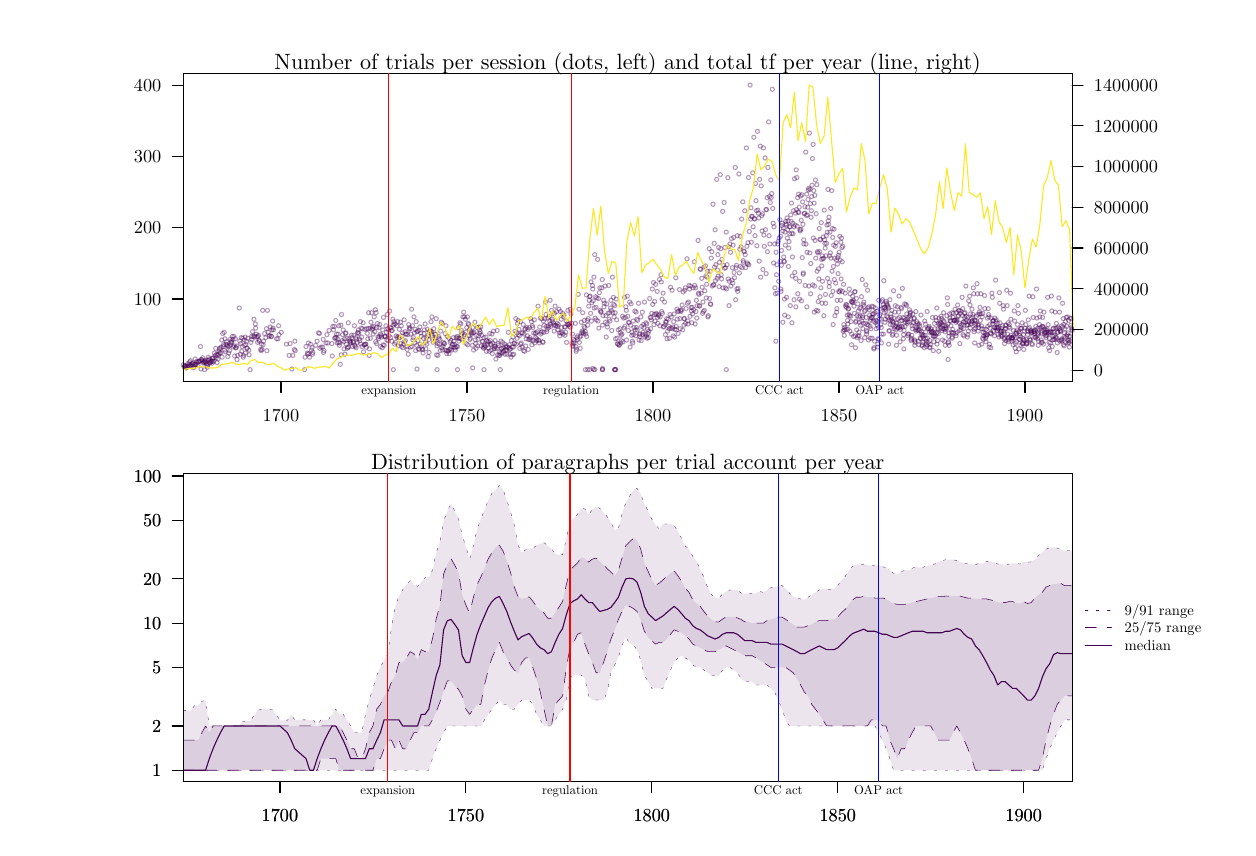
\begin{tikzpicture}[x=1pt,y=1pt]
\definecolor{fillColor}{RGB}{255,255,255}
\path[use as bounding box,fill=fillColor,fill opacity=0.00] (0,0) rectangle (433.62,289.08);
\begin{scope}
\path[clip] (  0.00,  0.00) rectangle (433.62,289.08);
\definecolor{drawColor}{RGB}{68,1,84}

\path[draw=drawColor,draw opacity=0.40,line width= 0.4pt,line join=round,line cap=round] ( 56.23,167.22) circle (  0.74);

\path[draw=drawColor,draw opacity=0.40,line width= 0.4pt,line join=round,line cap=round] ( 56.52,166.58) circle (  0.74);

\path[draw=drawColor,draw opacity=0.40,line width= 0.4pt,line join=round,line cap=round] ( 56.72,166.58) circle (  0.74);

\path[draw=drawColor,draw opacity=0.40,line width= 0.4pt,line join=round,line cap=round] ( 56.85,167.01) circle (  0.74);

\path[draw=drawColor,draw opacity=0.40,line width= 0.4pt,line join=round,line cap=round] ( 57.07,166.79) circle (  0.74);

\path[draw=drawColor,draw opacity=0.40,line width= 0.4pt,line join=round,line cap=round] ( 57.19,166.15) circle (  0.74);

\path[draw=drawColor,draw opacity=0.40,line width= 0.4pt,line join=round,line cap=round] ( 57.32,166.15) circle (  0.74);

\path[draw=drawColor,draw opacity=0.40,line width= 0.4pt,line join=round,line cap=round] ( 57.52,166.79) circle (  0.74);

\path[draw=drawColor,draw opacity=0.40,line width= 0.4pt,line join=round,line cap=round] ( 57.83,167.65) circle (  0.74);

\path[draw=drawColor,draw opacity=0.40,line width= 0.4pt,line join=round,line cap=round] ( 58.06,166.79) circle (  0.74);

\path[draw=drawColor,draw opacity=0.40,line width= 0.4pt,line join=round,line cap=round] ( 58.19,166.79) circle (  0.74);

\path[draw=drawColor,draw opacity=0.40,line width= 0.4pt,line join=round,line cap=round] ( 58.40,167.44) circle (  0.74);

\path[draw=drawColor,draw opacity=0.40,line width= 0.4pt,line join=round,line cap=round] ( 58.53,168.29) circle (  0.74);

\path[draw=drawColor,draw opacity=0.40,line width= 0.4pt,line join=round,line cap=round] ( 58.54,166.58) circle (  0.74);

\path[draw=drawColor,draw opacity=0.40,line width= 0.4pt,line join=round,line cap=round] ( 58.83,168.72) circle (  0.74);

\path[draw=drawColor,draw opacity=0.40,line width= 0.4pt,line join=round,line cap=round] ( 58.96,167.22) circle (  0.74);

\path[draw=drawColor,draw opacity=0.40,line width= 0.4pt,line join=round,line cap=round] ( 59.14,166.79) circle (  0.74);

\path[draw=drawColor,draw opacity=0.40,line width= 0.4pt,line join=round,line cap=round] ( 59.35,167.44) circle (  0.74);

\path[draw=drawColor,draw opacity=0.40,line width= 0.4pt,line join=round,line cap=round] ( 59.53,167.86) circle (  0.74);

\path[draw=drawColor,draw opacity=0.40,line width= 0.4pt,line join=round,line cap=round] ( 59.76,167.86) circle (  0.74);

\path[draw=drawColor,draw opacity=0.40,line width= 0.4pt,line join=round,line cap=round] ( 59.89,166.15) circle (  0.74);

\path[draw=drawColor,draw opacity=0.40,line width= 0.4pt,line join=round,line cap=round] ( 60.07,167.22) circle (  0.74);

\path[draw=drawColor,draw opacity=0.40,line width= 0.4pt,line join=round,line cap=round] ( 60.25,166.58) circle (  0.74);

\path[draw=drawColor,draw opacity=0.40,line width= 0.4pt,line join=round,line cap=round] ( 60.39,167.44) circle (  0.74);

\path[draw=drawColor,draw opacity=0.40,line width= 0.4pt,line join=round,line cap=round] ( 60.53,169.36) circle (  0.74);

\path[draw=drawColor,draw opacity=0.40,line width= 0.4pt,line join=round,line cap=round] ( 60.74,167.22) circle (  0.74);

\path[draw=drawColor,draw opacity=0.40,line width= 0.4pt,line join=round,line cap=round] ( 60.87,167.44) circle (  0.74);

\path[draw=drawColor,draw opacity=0.40,line width= 0.4pt,line join=round,line cap=round] ( 61.10,168.51) circle (  0.74);

\path[draw=drawColor,draw opacity=0.40,line width= 0.4pt,line join=round,line cap=round] ( 61.23,168.08) circle (  0.74);

\path[draw=drawColor,draw opacity=0.40,line width= 0.4pt,line join=round,line cap=round] ( 61.54,167.22) circle (  0.74);

\path[draw=drawColor,draw opacity=0.40,line width= 0.4pt,line join=round,line cap=round] ( 61.67,168.29) circle (  0.74);

\path[draw=drawColor,draw opacity=0.40,line width= 0.4pt,line join=round,line cap=round] ( 61.85,168.51) circle (  0.74);

\path[draw=drawColor,draw opacity=0.40,line width= 0.4pt,line join=round,line cap=round] ( 62.05,168.51) circle (  0.74);

\path[draw=drawColor,draw opacity=0.40,line width= 0.4pt,line join=round,line cap=round] ( 62.23,168.72) circle (  0.74);

\path[draw=drawColor,draw opacity=0.40,line width= 0.4pt,line join=round,line cap=round] ( 62.44,173.86) circle (  0.74);

\path[draw=drawColor,draw opacity=0.40,line width= 0.4pt,line join=round,line cap=round] ( 62.63,165.72) circle (  0.74);

\path[draw=drawColor,draw opacity=0.40,line width= 0.4pt,line join=round,line cap=round] ( 62.72,169.15) circle (  0.74);

\path[draw=drawColor,draw opacity=0.40,line width= 0.4pt,line join=round,line cap=round] ( 62.96,169.15) circle (  0.74);

\path[draw=drawColor,draw opacity=0.40,line width= 0.4pt,line join=round,line cap=round] ( 63.09,168.72) circle (  0.74);

\path[draw=drawColor,draw opacity=0.40,line width= 0.4pt,line join=round,line cap=round] ( 63.24,169.79) circle (  0.74);

\path[draw=drawColor,draw opacity=0.40,line width= 0.4pt,line join=round,line cap=round] ( 63.39,167.86) circle (  0.74);

\path[draw=drawColor,draw opacity=0.40,line width= 0.4pt,line join=round,line cap=round] ( 63.57,168.29) circle (  0.74);

\path[draw=drawColor,draw opacity=0.40,line width= 0.4pt,line join=round,line cap=round] ( 63.78,168.08) circle (  0.74);

\path[draw=drawColor,draw opacity=0.40,line width= 0.4pt,line join=round,line cap=round] ( 63.91,168.51) circle (  0.74);

\path[draw=drawColor,draw opacity=0.40,line width= 0.4pt,line join=round,line cap=round] ( 63.92,165.51) circle (  0.74);

\path[draw=drawColor,draw opacity=0.40,line width= 0.4pt,line join=round,line cap=round] ( 64.07,168.72) circle (  0.74);

\path[draw=drawColor,draw opacity=0.40,line width= 0.4pt,line join=round,line cap=round] ( 64.27,168.29) circle (  0.74);

\path[draw=drawColor,draw opacity=0.40,line width= 0.4pt,line join=round,line cap=round] ( 64.40,168.08) circle (  0.74);

\path[draw=drawColor,draw opacity=0.40,line width= 0.4pt,line join=round,line cap=round] ( 64.55,167.44) circle (  0.74);

\path[draw=drawColor,draw opacity=0.40,line width= 0.4pt,line join=round,line cap=round] ( 64.79,168.93) circle (  0.74);

\path[draw=drawColor,draw opacity=0.40,line width= 0.4pt,line join=round,line cap=round] ( 64.91,167.01) circle (  0.74);

\path[draw=drawColor,draw opacity=0.40,line width= 0.4pt,line join=round,line cap=round] ( 64.92,166.36) circle (  0.74);

\path[draw=drawColor,draw opacity=0.40,line width= 0.4pt,line join=round,line cap=round] ( 65.12,167.44) circle (  0.74);

\path[draw=drawColor,draw opacity=0.40,line width= 0.4pt,line join=round,line cap=round] ( 65.27,170.01) circle (  0.74);

\path[draw=drawColor,draw opacity=0.40,line width= 0.4pt,line join=round,line cap=round] ( 65.42,168.93) circle (  0.74);

\path[draw=drawColor,draw opacity=0.40,line width= 0.4pt,line join=round,line cap=round] ( 65.58,169.36) circle (  0.74);

\path[draw=drawColor,draw opacity=0.40,line width= 0.4pt,line join=round,line cap=round] ( 65.72,168.08) circle (  0.74);

\path[draw=drawColor,draw opacity=0.40,line width= 0.4pt,line join=round,line cap=round] ( 65.89,167.86) circle (  0.74);

\path[draw=drawColor,draw opacity=0.40,line width= 0.4pt,line join=round,line cap=round] ( 66.10,168.29) circle (  0.74);

\path[draw=drawColor,draw opacity=0.40,line width= 0.4pt,line join=round,line cap=round] ( 66.27,168.51) circle (  0.74);

\path[draw=drawColor,draw opacity=0.40,line width= 0.4pt,line join=round,line cap=round] ( 66.46,168.72) circle (  0.74);

\path[draw=drawColor,draw opacity=0.40,line width= 0.4pt,line join=round,line cap=round] ( 66.61,169.58) circle (  0.74);

\path[draw=drawColor,draw opacity=0.40,line width= 0.4pt,line join=round,line cap=round] ( 66.75,167.86) circle (  0.74);

\path[draw=drawColor,draw opacity=0.40,line width= 0.4pt,line join=round,line cap=round] ( 66.75,168.51) circle (  0.74);

\path[draw=drawColor,draw opacity=0.40,line width= 0.4pt,line join=round,line cap=round] ( 66.97,169.58) circle (  0.74);

\path[draw=drawColor,draw opacity=0.40,line width= 0.4pt,line join=round,line cap=round] ( 67.11,169.79) circle (  0.74);

\path[draw=drawColor,draw opacity=0.40,line width= 0.4pt,line join=round,line cap=round] ( 67.26,168.51) circle (  0.74);

\path[draw=drawColor,draw opacity=0.40,line width= 0.4pt,line join=round,line cap=round] ( 67.46,171.51) circle (  0.74);

\path[draw=drawColor,draw opacity=0.40,line width= 0.4pt,line join=round,line cap=round] ( 67.80,170.65) circle (  0.74);

\path[draw=drawColor,draw opacity=0.40,line width= 0.4pt,line join=round,line cap=round] ( 67.95,173.22) circle (  0.74);

\path[draw=drawColor,draw opacity=0.40,line width= 0.4pt,line join=round,line cap=round] ( 68.09,169.79) circle (  0.74);

\path[draw=drawColor,draw opacity=0.40,line width= 0.4pt,line join=round,line cap=round] ( 68.29,171.08) circle (  0.74);

\path[draw=drawColor,draw opacity=0.40,line width= 0.4pt,line join=round,line cap=round] ( 68.42,168.08) circle (  0.74);

\path[draw=drawColor,draw opacity=0.40,line width= 0.4pt,line join=round,line cap=round] ( 68.60,170.65) circle (  0.74);

\path[draw=drawColor,draw opacity=0.40,line width= 0.4pt,line join=round,line cap=round] ( 68.78,169.36) circle (  0.74);

\path[draw=drawColor,draw opacity=0.40,line width= 0.4pt,line join=round,line cap=round] ( 68.93,171.08) circle (  0.74);

\path[draw=drawColor,draw opacity=0.40,line width= 0.4pt,line join=round,line cap=round] ( 69.16,172.15) circle (  0.74);

\path[draw=drawColor,draw opacity=0.40,line width= 0.4pt,line join=round,line cap=round] ( 69.29,173.00) circle (  0.74);

\path[draw=drawColor,draw opacity=0.40,line width= 0.4pt,line join=round,line cap=round] ( 69.45,171.51) circle (  0.74);

\path[draw=drawColor,draw opacity=0.40,line width= 0.4pt,line join=round,line cap=round] ( 69.60,173.22) circle (  0.74);

\path[draw=drawColor,draw opacity=0.40,line width= 0.4pt,line join=round,line cap=round] ( 69.73,171.51) circle (  0.74);

\path[draw=drawColor,draw opacity=0.40,line width= 0.4pt,line join=round,line cap=round] ( 69.91,173.65) circle (  0.74);

\path[draw=drawColor,draw opacity=0.40,line width= 0.4pt,line join=round,line cap=round] ( 70.14,176.22) circle (  0.74);

\path[draw=drawColor,draw opacity=0.40,line width= 0.4pt,line join=round,line cap=round] ( 70.27,170.01) circle (  0.74);

\path[draw=drawColor,draw opacity=0.40,line width= 0.4pt,line join=round,line cap=round] ( 70.50,178.57) circle (  0.74);

\path[draw=drawColor,draw opacity=0.40,line width= 0.4pt,line join=round,line cap=round] ( 70.64,173.86) circle (  0.74);

\path[draw=drawColor,draw opacity=0.40,line width= 0.4pt,line join=round,line cap=round] ( 70.79,174.50) circle (  0.74);

\path[draw=drawColor,draw opacity=0.40,line width= 0.4pt,line join=round,line cap=round] ( 71.02,179.00) circle (  0.74);

\path[draw=drawColor,draw opacity=0.40,line width= 0.4pt,line join=round,line cap=round] ( 71.15,172.58) circle (  0.74);

\path[draw=drawColor,draw opacity=0.40,line width= 0.4pt,line join=round,line cap=round] ( 71.31,176.65) circle (  0.74);

\path[draw=drawColor,draw opacity=0.40,line width= 0.4pt,line join=round,line cap=round] ( 71.46,171.93) circle (  0.74);

\path[draw=drawColor,draw opacity=0.40,line width= 0.4pt,line join=round,line cap=round] ( 71.64,174.72) circle (  0.74);

\path[draw=drawColor,draw opacity=0.40,line width= 0.4pt,line join=round,line cap=round] ( 71.84,175.58) circle (  0.74);

\path[draw=drawColor,draw opacity=0.40,line width= 0.4pt,line join=round,line cap=round] ( 71.98,174.50) circle (  0.74);

\path[draw=drawColor,draw opacity=0.40,line width= 0.4pt,line join=round,line cap=round] ( 72.13,174.08) circle (  0.74);

\path[draw=drawColor,draw opacity=0.40,line width= 0.4pt,line join=round,line cap=round] ( 72.31,170.22) circle (  0.74);

\path[draw=drawColor,draw opacity=0.40,line width= 0.4pt,line join=round,line cap=round] ( 72.44,173.86) circle (  0.74);

\path[draw=drawColor,draw opacity=0.40,line width= 0.4pt,line join=round,line cap=round] ( 72.62,171.51) circle (  0.74);

\path[draw=drawColor,draw opacity=0.40,line width= 0.4pt,line join=round,line cap=round] ( 72.82,174.08) circle (  0.74);

\path[draw=drawColor,draw opacity=0.40,line width= 0.4pt,line join=round,line cap=round] ( 72.98,172.36) circle (  0.74);

\path[draw=drawColor,draw opacity=0.40,line width= 0.4pt,line join=round,line cap=round] ( 73.18,176.43) circle (  0.74);

\path[draw=drawColor,draw opacity=0.40,line width= 0.4pt,line join=round,line cap=round] ( 73.32,174.50) circle (  0.74);

\path[draw=drawColor,draw opacity=0.40,line width= 0.4pt,line join=round,line cap=round] ( 73.47,175.36) circle (  0.74);

\path[draw=drawColor,draw opacity=0.40,line width= 0.4pt,line join=round,line cap=round] ( 73.62,175.79) circle (  0.74);

\path[draw=drawColor,draw opacity=0.40,line width= 0.4pt,line join=round,line cap=round] ( 73.75,175.36) circle (  0.74);

\path[draw=drawColor,draw opacity=0.40,line width= 0.4pt,line join=round,line cap=round] ( 73.94,177.50) circle (  0.74);

\path[draw=drawColor,draw opacity=0.40,line width= 0.4pt,line join=round,line cap=round] ( 74.16,176.43) circle (  0.74);

\path[draw=drawColor,draw opacity=0.40,line width= 0.4pt,line join=round,line cap=round] ( 74.32,173.65) circle (  0.74);

\path[draw=drawColor,draw opacity=0.40,line width= 0.4pt,line join=round,line cap=round] ( 74.52,177.50) circle (  0.74);

\path[draw=drawColor,draw opacity=0.40,line width= 0.4pt,line join=round,line cap=round] ( 74.66,174.08) circle (  0.74);

\path[draw=drawColor,draw opacity=0.40,line width= 0.4pt,line join=round,line cap=round] ( 74.81,170.43) circle (  0.74);

\path[draw=drawColor,draw opacity=0.40,line width= 0.4pt,line join=round,line cap=round] ( 75.04,176.65) circle (  0.74);

\path[draw=drawColor,draw opacity=0.40,line width= 0.4pt,line join=round,line cap=round] ( 75.17,173.43) circle (  0.74);

\path[draw=drawColor,draw opacity=0.40,line width= 0.4pt,line join=round,line cap=round] ( 75.32,173.43) circle (  0.74);

\path[draw=drawColor,draw opacity=0.40,line width= 0.4pt,line join=round,line cap=round] ( 75.51,174.08) circle (  0.74);

\path[draw=drawColor,draw opacity=0.40,line width= 0.4pt,line join=round,line cap=round] ( 75.66,169.15) circle (  0.74);

\path[draw=drawColor,draw opacity=0.40,line width= 0.4pt,line join=round,line cap=round] ( 75.86,170.65) circle (  0.74);

\path[draw=drawColor,draw opacity=0.40,line width= 0.4pt,line join=round,line cap=round] ( 76.46,187.79) circle (  0.74);

\path[draw=drawColor,draw opacity=0.40,line width= 0.4pt,line join=round,line cap=round] ( 76.64,175.79) circle (  0.74);

\path[draw=drawColor,draw opacity=0.40,line width= 0.4pt,line join=round,line cap=round] ( 76.84,171.08) circle (  0.74);

\path[draw=drawColor,draw opacity=0.40,line width= 0.4pt,line join=round,line cap=round] ( 77.00,174.93) circle (  0.74);

\path[draw=drawColor,draw opacity=0.40,line width= 0.4pt,line join=round,line cap=round] ( 77.23,177.07) circle (  0.74);

\path[draw=drawColor,draw opacity=0.40,line width= 0.4pt,line join=round,line cap=round] ( 77.36,172.15) circle (  0.74);

\path[draw=drawColor,draw opacity=0.40,line width= 0.4pt,line join=round,line cap=round] ( 77.51,173.86) circle (  0.74);

\path[draw=drawColor,draw opacity=0.40,line width= 0.4pt,line join=round,line cap=round] ( 77.74,176.86) circle (  0.74);

\path[draw=drawColor,draw opacity=0.40,line width= 0.4pt,line join=round,line cap=round] ( 77.88,170.01) circle (  0.74);

\path[draw=drawColor,draw opacity=0.40,line width= 0.4pt,line join=round,line cap=round] ( 78.03,170.65) circle (  0.74);

\path[draw=drawColor,draw opacity=0.40,line width= 0.4pt,line join=round,line cap=round] ( 78.21,176.22) circle (  0.74);

\path[draw=drawColor,draw opacity=0.40,line width= 0.4pt,line join=round,line cap=round] ( 78.36,174.29) circle (  0.74);

\path[draw=drawColor,draw opacity=0.40,line width= 0.4pt,line join=round,line cap=round] ( 78.57,177.29) circle (  0.74);

\path[draw=drawColor,draw opacity=0.40,line width= 0.4pt,line join=round,line cap=round] ( 78.70,171.51) circle (  0.74);

\path[draw=drawColor,draw opacity=0.40,line width= 0.4pt,line join=round,line cap=round] ( 78.83,174.50) circle (  0.74);

\path[draw=drawColor,draw opacity=0.40,line width= 0.4pt,line join=round,line cap=round] ( 79.06,175.79) circle (  0.74);

\path[draw=drawColor,draw opacity=0.40,line width= 0.4pt,line join=round,line cap=round] ( 79.19,173.22) circle (  0.74);

\path[draw=drawColor,draw opacity=0.40,line width= 0.4pt,line join=round,line cap=round] ( 79.34,173.22) circle (  0.74);

\path[draw=drawColor,draw opacity=0.40,line width= 0.4pt,line join=round,line cap=round] ( 79.57,176.86) circle (  0.74);

\path[draw=drawColor,draw opacity=0.40,line width= 0.4pt,line join=round,line cap=round] ( 79.91,172.58) circle (  0.74);

\path[draw=drawColor,draw opacity=0.40,line width= 0.4pt,line join=round,line cap=round] ( 80.04,170.86) circle (  0.74);

\path[draw=drawColor,draw opacity=0.40,line width= 0.4pt,line join=round,line cap=round] ( 80.35,165.51) circle (  0.74);

\path[draw=drawColor,draw opacity=0.40,line width= 0.4pt,line join=round,line cap=round] ( 80.65,175.36) circle (  0.74);

\path[draw=drawColor,draw opacity=0.40,line width= 0.4pt,line join=round,line cap=round] ( 80.89,177.50) circle (  0.74);

\path[draw=drawColor,draw opacity=0.40,line width= 0.4pt,line join=round,line cap=round] ( 81.04,176.43) circle (  0.74);

\path[draw=drawColor,draw opacity=0.40,line width= 0.4pt,line join=round,line cap=round] ( 81.25,179.22) circle (  0.74);

\path[draw=drawColor,draw opacity=0.40,line width= 0.4pt,line join=round,line cap=round] ( 81.39,177.50) circle (  0.74);

\path[draw=drawColor,draw opacity=0.40,line width= 0.4pt,line join=round,line cap=round] ( 81.76,183.72) circle (  0.74);

\path[draw=drawColor,draw opacity=0.40,line width= 0.4pt,line join=round,line cap=round] ( 81.89,177.72) circle (  0.74);

\path[draw=drawColor,draw opacity=0.40,line width= 0.4pt,line join=round,line cap=round] ( 82.05,177.29) circle (  0.74);

\path[draw=drawColor,draw opacity=0.40,line width= 0.4pt,line join=round,line cap=round] ( 82.25,182.00) circle (  0.74);

\path[draw=drawColor,draw opacity=0.40,line width= 0.4pt,line join=round,line cap=round] ( 82.38,180.50) circle (  0.74);

\path[draw=drawColor,draw opacity=0.40,line width= 0.4pt,line join=round,line cap=round] ( 82.59,178.36) circle (  0.74);

\path[draw=drawColor,draw opacity=0.40,line width= 0.4pt,line join=round,line cap=round] ( 82.87,177.29) circle (  0.74);

\path[draw=drawColor,draw opacity=0.40,line width= 0.4pt,line join=round,line cap=round] ( 83.08,175.36) circle (  0.74);

\path[draw=drawColor,draw opacity=0.40,line width= 0.4pt,line join=round,line cap=round] ( 83.21,177.50) circle (  0.74);

\path[draw=drawColor,draw opacity=0.40,line width= 0.4pt,line join=round,line cap=round] ( 83.39,177.93) circle (  0.74);

\path[draw=drawColor,draw opacity=0.40,line width= 0.4pt,line join=round,line cap=round] ( 83.57,176.22) circle (  0.74);

\path[draw=drawColor,draw opacity=0.40,line width= 0.4pt,line join=round,line cap=round] ( 83.72,175.79) circle (  0.74);

\path[draw=drawColor,draw opacity=0.40,line width= 0.4pt,line join=round,line cap=round] ( 84.21,172.79) circle (  0.74);

\path[draw=drawColor,draw opacity=0.40,line width= 0.4pt,line join=round,line cap=round] ( 84.36,172.36) circle (  0.74);

\path[draw=drawColor,draw opacity=0.40,line width= 0.4pt,line join=round,line cap=round] ( 84.49,174.72) circle (  0.74);

\path[draw=drawColor,draw opacity=0.40,line width= 0.4pt,line join=round,line cap=round] ( 84.70,172.79) circle (  0.74);

\path[draw=drawColor,draw opacity=0.40,line width= 0.4pt,line join=round,line cap=round] ( 84.91,186.93) circle (  0.74);

\path[draw=drawColor,draw opacity=0.40,line width= 0.4pt,line join=round,line cap=round] ( 85.08,174.50) circle (  0.74);

\path[draw=drawColor,draw opacity=0.40,line width= 0.4pt,line join=round,line cap=round] ( 85.26,175.79) circle (  0.74);

\path[draw=drawColor,draw opacity=0.40,line width= 0.4pt,line join=round,line cap=round] ( 85.58,178.57) circle (  0.74);

\path[draw=drawColor,draw opacity=0.40,line width= 0.4pt,line join=round,line cap=round] ( 86.06,177.07) circle (  0.74);

\path[draw=drawColor,draw opacity=0.40,line width= 0.4pt,line join=round,line cap=round] ( 86.30,180.29) circle (  0.74);

\path[draw=drawColor,draw opacity=0.40,line width= 0.4pt,line join=round,line cap=round] ( 86.43,172.36) circle (  0.74);

\path[draw=drawColor,draw opacity=0.40,line width= 0.4pt,line join=round,line cap=round] ( 86.63,186.93) circle (  0.74);

\path[draw=drawColor,draw opacity=0.40,line width= 0.4pt,line join=round,line cap=round] ( 86.91,179.00) circle (  0.74);

\path[draw=drawColor,draw opacity=0.40,line width= 0.4pt,line join=round,line cap=round] ( 87.22,177.50) circle (  0.74);

\path[draw=drawColor,draw opacity=0.40,line width= 0.4pt,line join=round,line cap=round] ( 87.40,177.93) circle (  0.74);

\path[draw=drawColor,draw opacity=0.40,line width= 0.4pt,line join=round,line cap=round] ( 87.61,180.93) circle (  0.74);

\path[draw=drawColor,draw opacity=0.40,line width= 0.4pt,line join=round,line cap=round] ( 87.97,177.50) circle (  0.74);

\path[draw=drawColor,draw opacity=0.40,line width= 0.4pt,line join=round,line cap=round] ( 88.11,177.50) circle (  0.74);

\path[draw=drawColor,draw opacity=0.40,line width= 0.4pt,line join=round,line cap=round] ( 88.25,179.86) circle (  0.74);

\path[draw=drawColor,draw opacity=0.40,line width= 0.4pt,line join=round,line cap=round] ( 88.51,183.07) circle (  0.74);

\path[draw=drawColor,draw opacity=0.40,line width= 0.4pt,line join=round,line cap=round] ( 88.64,180.50) circle (  0.74);

\path[draw=drawColor,draw opacity=0.40,line width= 0.4pt,line join=round,line cap=round] ( 88.80,179.86) circle (  0.74);

\path[draw=drawColor,draw opacity=0.40,line width= 0.4pt,line join=round,line cap=round] ( 89.93,176.65) circle (  0.74);

\path[draw=drawColor,draw opacity=0.40,line width= 0.4pt,line join=round,line cap=round] ( 90.44,176.65) circle (  0.74);

\path[draw=drawColor,draw opacity=0.40,line width= 0.4pt,line join=round,line cap=round] ( 90.68,181.36) circle (  0.74);

\path[draw=drawColor,draw opacity=0.40,line width= 0.4pt,line join=round,line cap=round] ( 90.80,178.15) circle (  0.74);

\path[draw=drawColor,draw opacity=0.40,line width= 0.4pt,line join=round,line cap=round] ( 91.63,179.00) circle (  0.74);

\path[draw=drawColor,draw opacity=0.40,line width= 0.4pt,line join=round,line cap=round] ( 93.48,174.72) circle (  0.74);

\path[draw=drawColor,draw opacity=0.40,line width= 0.4pt,line join=round,line cap=round] ( 94.48,170.65) circle (  0.74);

\path[draw=drawColor,draw opacity=0.40,line width= 0.4pt,line join=round,line cap=round] ( 94.83,174.93) circle (  0.74);

\path[draw=drawColor,draw opacity=0.40,line width= 0.4pt,line join=round,line cap=round] ( 95.46,165.72) circle (  0.74);

\path[draw=drawColor,draw opacity=0.40,line width= 0.4pt,line join=round,line cap=round] ( 95.82,170.65) circle (  0.74);

\path[draw=drawColor,draw opacity=0.40,line width= 0.4pt,line join=round,line cap=round] ( 96.37,172.79) circle (  0.74);

\path[draw=drawColor,draw opacity=0.40,line width= 0.4pt,line join=round,line cap=round] ( 96.55,175.79) circle (  0.74);

\path[draw=drawColor,draw opacity=0.40,line width= 0.4pt,line join=round,line cap=round] ( 96.68,172.36) circle (  0.74);

\path[draw=drawColor,draw opacity=0.40,line width= 0.4pt,line join=round,line cap=round] (100.06,165.51) circle (  0.74);

\path[draw=drawColor,draw opacity=0.40,line width= 0.4pt,line join=round,line cap=round] (100.20,170.01) circle (  0.74);

\path[draw=drawColor,draw opacity=0.40,line width= 0.4pt,line join=round,line cap=round] (100.56,173.86) circle (  0.74);

\path[draw=drawColor,draw opacity=0.40,line width= 0.4pt,line join=round,line cap=round] (101.05,171.51) circle (  0.74);

\path[draw=drawColor,draw opacity=0.40,line width= 0.4pt,line join=round,line cap=round] (101.21,171.08) circle (  0.74);

\path[draw=drawColor,draw opacity=0.40,line width= 0.4pt,line join=round,line cap=round] (101.41,175.15) circle (  0.74);

\path[draw=drawColor,draw opacity=0.40,line width= 0.4pt,line join=round,line cap=round] (101.55,171.29) circle (  0.74);

\path[draw=drawColor,draw opacity=0.40,line width= 0.4pt,line join=round,line cap=round] (101.88,170.01) circle (  0.74);

\path[draw=drawColor,draw opacity=0.40,line width= 0.4pt,line join=round,line cap=round] (102.19,174.72) circle (  0.74);

\path[draw=drawColor,draw opacity=0.40,line width= 0.4pt,line join=round,line cap=round] (102.55,172.58) circle (  0.74);

\path[draw=drawColor,draw opacity=0.40,line width= 0.4pt,line join=round,line cap=round] (102.75,173.43) circle (  0.74);

\path[draw=drawColor,draw opacity=0.40,line width= 0.4pt,line join=round,line cap=round] (102.90,171.08) circle (  0.74);

\path[draw=drawColor,draw opacity=0.40,line width= 0.4pt,line join=round,line cap=round] (103.06,171.72) circle (  0.74);

\path[draw=drawColor,draw opacity=0.40,line width= 0.4pt,line join=round,line cap=round] (104.09,174.29) circle (  0.74);

\path[draw=drawColor,draw opacity=0.40,line width= 0.4pt,line join=round,line cap=round] (104.58,175.79) circle (  0.74);

\path[draw=drawColor,draw opacity=0.40,line width= 0.4pt,line join=round,line cap=round] (105.10,178.79) circle (  0.74);

\path[draw=drawColor,draw opacity=0.40,line width= 0.4pt,line join=round,line cap=round] (105.43,178.57) circle (  0.74);

\path[draw=drawColor,draw opacity=0.40,line width= 0.4pt,line join=round,line cap=round] (105.57,173.22) circle (  0.74);

\path[draw=drawColor,draw opacity=0.40,line width= 0.4pt,line join=round,line cap=round] (106.03,173.65) circle (  0.74);

\path[draw=drawColor,draw opacity=0.40,line width= 0.4pt,line join=round,line cap=round] (106.57,173.65) circle (  0.74);

\path[draw=drawColor,draw opacity=0.40,line width= 0.4pt,line join=round,line cap=round] (106.77,176.43) circle (  0.74);

\path[draw=drawColor,draw opacity=0.40,line width= 0.4pt,line join=round,line cap=round] (106.91,171.72) circle (  0.74);

\path[draw=drawColor,draw opacity=0.40,line width= 0.4pt,line join=round,line cap=round] (107.08,172.36) circle (  0.74);

\path[draw=drawColor,draw opacity=0.40,line width= 0.4pt,line join=round,line cap=round] (107.80,175.15) circle (  0.74);

\path[draw=drawColor,draw opacity=0.40,line width= 0.4pt,line join=round,line cap=round] (108.14,178.15) circle (  0.74);

\path[draw=drawColor,draw opacity=0.40,line width= 0.4pt,line join=round,line cap=round] (108.42,175.15) circle (  0.74);

\path[draw=drawColor,draw opacity=0.40,line width= 0.4pt,line join=round,line cap=round] (108.91,179.65) circle (  0.74);

\path[draw=drawColor,draw opacity=0.40,line width= 0.4pt,line join=round,line cap=round] (109.92,174.93) circle (  0.74);

\path[draw=drawColor,draw opacity=0.40,line width= 0.4pt,line join=round,line cap=round] (110.05,170.43) circle (  0.74);

\path[draw=drawColor,draw opacity=0.40,line width= 0.4pt,line join=round,line cap=round] (110.23,181.14) circle (  0.74);

\path[draw=drawColor,draw opacity=0.40,line width= 0.4pt,line join=round,line cap=round] (110.48,179.86) circle (  0.74);

\path[draw=drawColor,draw opacity=0.40,line width= 0.4pt,line join=round,line cap=round] (110.82,181.14) circle (  0.74);

\path[draw=drawColor,draw opacity=0.40,line width= 0.4pt,line join=round,line cap=round] (110.95,176.86) circle (  0.74);

\path[draw=drawColor,draw opacity=0.40,line width= 0.4pt,line join=round,line cap=round] (111.10,177.07) circle (  0.74);

\path[draw=drawColor,draw opacity=0.40,line width= 0.4pt,line join=round,line cap=round] (111.33,183.29) circle (  0.74);

\path[draw=drawColor,draw opacity=0.40,line width= 0.4pt,line join=round,line cap=round] (111.47,177.07) circle (  0.74);

\path[draw=drawColor,draw opacity=0.40,line width= 0.4pt,line join=round,line cap=round] (111.62,178.36) circle (  0.74);

\path[draw=drawColor,draw opacity=0.40,line width= 0.4pt,line join=round,line cap=round] (111.82,175.15) circle (  0.74);

\path[draw=drawColor,draw opacity=0.40,line width= 0.4pt,line join=round,line cap=round] (111.95,176.65) circle (  0.74);

\path[draw=drawColor,draw opacity=0.40,line width= 0.4pt,line join=round,line cap=round] (112.16,178.36) circle (  0.74);

\path[draw=drawColor,draw opacity=0.40,line width= 0.4pt,line join=round,line cap=round] (112.29,175.36) circle (  0.74);

\path[draw=drawColor,draw opacity=0.40,line width= 0.4pt,line join=round,line cap=round] (112.44,181.36) circle (  0.74);

\path[draw=drawColor,draw opacity=0.40,line width= 0.4pt,line join=round,line cap=round] (112.62,174.29) circle (  0.74);

\path[draw=drawColor,draw opacity=0.40,line width= 0.4pt,line join=round,line cap=round] (112.75,175.15) circle (  0.74);

\path[draw=drawColor,draw opacity=0.40,line width= 0.4pt,line join=round,line cap=round] (112.96,167.44) circle (  0.74);

\path[draw=drawColor,draw opacity=0.40,line width= 0.4pt,line join=round,line cap=round] (113.17,181.57) circle (  0.74);

\path[draw=drawColor,draw opacity=0.40,line width= 0.4pt,line join=round,line cap=round] (113.29,170.86) circle (  0.74);

\path[draw=drawColor,draw opacity=0.40,line width= 0.4pt,line join=round,line cap=round] (113.39,185.43) circle (  0.74);

\path[draw=drawColor,draw opacity=0.40,line width= 0.4pt,line join=round,line cap=round] (113.63,176.00) circle (  0.74);

\path[draw=drawColor,draw opacity=0.40,line width= 0.4pt,line join=round,line cap=round] (113.81,178.15) circle (  0.74);

\path[draw=drawColor,draw opacity=0.40,line width= 0.4pt,line join=round,line cap=round] (114.04,179.86) circle (  0.74);

\path[draw=drawColor,draw opacity=0.40,line width= 0.4pt,line join=round,line cap=round] (114.17,175.58) circle (  0.74);

\path[draw=drawColor,draw opacity=0.40,line width= 0.4pt,line join=round,line cap=round] (114.32,173.00) circle (  0.74);

\path[draw=drawColor,draw opacity=0.40,line width= 0.4pt,line join=round,line cap=round] (114.53,176.65) circle (  0.74);

\path[draw=drawColor,draw opacity=0.40,line width= 0.4pt,line join=round,line cap=round] (114.66,171.08) circle (  0.74);

\path[draw=drawColor,draw opacity=0.40,line width= 0.4pt,line join=round,line cap=round] (114.84,178.57) circle (  0.74);

\path[draw=drawColor,draw opacity=0.40,line width= 0.4pt,line join=round,line cap=round] (114.97,178.79) circle (  0.74);

\path[draw=drawColor,draw opacity=0.40,line width= 0.4pt,line join=round,line cap=round] (115.15,174.72) circle (  0.74);

\path[draw=drawColor,draw opacity=0.40,line width= 0.4pt,line join=round,line cap=round] (115.35,176.86) circle (  0.74);

\path[draw=drawColor,draw opacity=0.40,line width= 0.4pt,line join=round,line cap=round] (115.49,173.22) circle (  0.74);

\path[draw=drawColor,draw opacity=0.40,line width= 0.4pt,line join=round,line cap=round] (115.64,173.65) circle (  0.74);

\path[draw=drawColor,draw opacity=0.40,line width= 0.4pt,line join=round,line cap=round] (115.87,182.43) circle (  0.74);

\path[draw=drawColor,draw opacity=0.40,line width= 0.4pt,line join=round,line cap=round] (116.00,173.65) circle (  0.74);

\path[draw=drawColor,draw opacity=0.40,line width= 0.4pt,line join=round,line cap=round] (116.18,176.65) circle (  0.74);

\path[draw=drawColor,draw opacity=0.40,line width= 0.4pt,line join=round,line cap=round] (116.33,175.79) circle (  0.74);

\path[draw=drawColor,draw opacity=0.40,line width= 0.4pt,line join=round,line cap=round] (116.49,175.79) circle (  0.74);

\path[draw=drawColor,draw opacity=0.40,line width= 0.4pt,line join=round,line cap=round] (116.64,175.15) circle (  0.74);

\path[draw=drawColor,draw opacity=0.40,line width= 0.4pt,line join=round,line cap=round] (116.77,175.36) circle (  0.74);

\path[draw=drawColor,draw opacity=0.40,line width= 0.4pt,line join=round,line cap=round] (116.98,177.93) circle (  0.74);

\path[draw=drawColor,draw opacity=0.40,line width= 0.4pt,line join=round,line cap=round] (117.18,177.07) circle (  0.74);

\path[draw=drawColor,draw opacity=0.40,line width= 0.4pt,line join=round,line cap=round] (117.34,173.86) circle (  0.74);

\path[draw=drawColor,draw opacity=0.40,line width= 0.4pt,line join=round,line cap=round] (117.52,175.58) circle (  0.74);

\path[draw=drawColor,draw opacity=0.40,line width= 0.4pt,line join=round,line cap=round] (117.68,175.36) circle (  0.74);

\path[draw=drawColor,draw opacity=0.40,line width= 0.4pt,line join=round,line cap=round] (117.85,177.93) circle (  0.74);

\path[draw=drawColor,draw opacity=0.40,line width= 0.4pt,line join=round,line cap=round] (118.06,181.36) circle (  0.74);

\path[draw=drawColor,draw opacity=0.40,line width= 0.4pt,line join=round,line cap=round] (118.19,174.29) circle (  0.74);

\path[draw=drawColor,draw opacity=0.40,line width= 0.4pt,line join=round,line cap=round] (118.34,173.86) circle (  0.74);

\path[draw=drawColor,draw opacity=0.40,line width= 0.4pt,line join=round,line cap=round] (118.55,177.07) circle (  0.74);

\path[draw=drawColor,draw opacity=0.40,line width= 0.4pt,line join=round,line cap=round] (118.68,173.43) circle (  0.74);

\path[draw=drawColor,draw opacity=0.40,line width= 0.4pt,line join=round,line cap=round] (118.88,176.43) circle (  0.74);

\path[draw=drawColor,draw opacity=0.40,line width= 0.4pt,line join=round,line cap=round] (119.02,175.36) circle (  0.74);

\path[draw=drawColor,draw opacity=0.40,line width= 0.4pt,line join=round,line cap=round] (119.19,178.79) circle (  0.74);

\path[draw=drawColor,draw opacity=0.40,line width= 0.4pt,line join=round,line cap=round] (119.37,179.00) circle (  0.74);

\path[draw=drawColor,draw opacity=0.40,line width= 0.4pt,line join=round,line cap=round] (119.50,179.86) circle (  0.74);

\path[draw=drawColor,draw opacity=0.40,line width= 0.4pt,line join=round,line cap=round] (119.68,178.57) circle (  0.74);

\path[draw=drawColor,draw opacity=0.40,line width= 0.4pt,line join=round,line cap=round] (119.86,176.65) circle (  0.74);

\path[draw=drawColor,draw opacity=0.40,line width= 0.4pt,line join=round,line cap=round] (120.01,176.00) circle (  0.74);

\path[draw=drawColor,draw opacity=0.40,line width= 0.4pt,line join=round,line cap=round] (120.22,182.86) circle (  0.74);

\path[draw=drawColor,draw opacity=0.40,line width= 0.4pt,line join=round,line cap=round] (120.36,174.72) circle (  0.74);

\path[draw=drawColor,draw opacity=0.40,line width= 0.4pt,line join=round,line cap=round] (120.53,180.50) circle (  0.74);

\path[draw=drawColor,draw opacity=0.40,line width= 0.4pt,line join=round,line cap=round] (120.66,177.29) circle (  0.74);

\path[draw=drawColor,draw opacity=0.40,line width= 0.4pt,line join=round,line cap=round] (120.79,173.86) circle (  0.74);

\path[draw=drawColor,draw opacity=0.40,line width= 0.4pt,line join=round,line cap=round] (120.99,180.29) circle (  0.74);

\path[draw=drawColor,draw opacity=0.40,line width= 0.4pt,line join=round,line cap=round] (121.23,182.43) circle (  0.74);

\path[draw=drawColor,draw opacity=0.40,line width= 0.4pt,line join=round,line cap=round] (121.35,171.93) circle (  0.74);

\path[draw=drawColor,draw opacity=0.40,line width= 0.4pt,line join=round,line cap=round] (121.56,174.50) circle (  0.74);

\path[draw=drawColor,draw opacity=0.40,line width= 0.4pt,line join=round,line cap=round] (121.72,174.50) circle (  0.74);

\path[draw=drawColor,draw opacity=0.40,line width= 0.4pt,line join=round,line cap=round] (121.87,180.07) circle (  0.74);

\path[draw=drawColor,draw opacity=0.40,line width= 0.4pt,line join=round,line cap=round] (122.08,174.72) circle (  0.74);

\path[draw=drawColor,draw opacity=0.40,line width= 0.4pt,line join=round,line cap=round] (122.21,174.72) circle (  0.74);

\path[draw=drawColor,draw opacity=0.40,line width= 0.4pt,line join=round,line cap=round] (122.36,173.65) circle (  0.74);

\path[draw=drawColor,draw opacity=0.40,line width= 0.4pt,line join=round,line cap=round] (122.54,180.29) circle (  0.74);

\path[draw=drawColor,draw opacity=0.40,line width= 0.4pt,line join=round,line cap=round] (122.72,178.57) circle (  0.74);

\path[draw=drawColor,draw opacity=0.40,line width= 0.4pt,line join=round,line cap=round] (122.90,176.65) circle (  0.74);

\path[draw=drawColor,draw opacity=0.40,line width= 0.4pt,line join=round,line cap=round] (123.06,180.29) circle (  0.74);

\path[draw=drawColor,draw opacity=0.40,line width= 0.4pt,line join=round,line cap=round] (123.21,186.07) circle (  0.74);

\path[draw=drawColor,draw opacity=0.40,line width= 0.4pt,line join=round,line cap=round] (123.39,170.65) circle (  0.74);

\path[draw=drawColor,draw opacity=0.40,line width= 0.4pt,line join=round,line cap=round] (123.52,173.00) circle (  0.74);

\path[draw=drawColor,draw opacity=0.40,line width= 0.4pt,line join=round,line cap=round] (123.70,180.50) circle (  0.74);

\path[draw=drawColor,draw opacity=0.40,line width= 0.4pt,line join=round,line cap=round] (123.83,176.86) circle (  0.74);

\path[draw=drawColor,draw opacity=0.40,line width= 0.4pt,line join=round,line cap=round] (124.06,182.64) circle (  0.74);

\path[draw=drawColor,draw opacity=0.40,line width= 0.4pt,line join=round,line cap=round] (124.25,186.07) circle (  0.74);

\path[draw=drawColor,draw opacity=0.40,line width= 0.4pt,line join=round,line cap=round] (124.40,180.07) circle (  0.74);

\path[draw=drawColor,draw opacity=0.40,line width= 0.4pt,line join=round,line cap=round] (124.55,180.93) circle (  0.74);

\path[draw=drawColor,draw opacity=0.40,line width= 0.4pt,line join=round,line cap=round] (124.70,180.29) circle (  0.74);

\path[draw=drawColor,draw opacity=0.40,line width= 0.4pt,line join=round,line cap=round] (124.84,178.36) circle (  0.74);

\path[draw=drawColor,draw opacity=0.40,line width= 0.4pt,line join=round,line cap=round] (125.01,181.14) circle (  0.74);

\path[draw=drawColor,draw opacity=0.40,line width= 0.4pt,line join=round,line cap=round] (125.23,184.57) circle (  0.74);

\path[draw=drawColor,draw opacity=0.40,line width= 0.4pt,line join=round,line cap=round] (125.40,179.22) circle (  0.74);

\path[draw=drawColor,draw opacity=0.40,line width= 0.4pt,line join=round,line cap=round] (125.61,187.14) circle (  0.74);

\path[draw=drawColor,draw opacity=0.40,line width= 0.4pt,line join=round,line cap=round] (125.74,175.58) circle (  0.74);

\path[draw=drawColor,draw opacity=0.40,line width= 0.4pt,line join=round,line cap=round] (125.91,186.07) circle (  0.74);

\path[draw=drawColor,draw opacity=0.40,line width= 0.4pt,line join=round,line cap=round] (126.09,180.72) circle (  0.74);

\path[draw=drawColor,draw opacity=0.40,line width= 0.4pt,line join=round,line cap=round] (126.11,174.93) circle (  0.74);

\path[draw=drawColor,draw opacity=0.40,line width= 0.4pt,line join=round,line cap=round] (126.40,182.22) circle (  0.74);

\path[draw=drawColor,draw opacity=0.40,line width= 0.4pt,line join=round,line cap=round] (126.58,177.29) circle (  0.74);

\path[draw=drawColor,draw opacity=0.40,line width= 0.4pt,line join=round,line cap=round] (126.74,176.65) circle (  0.74);

\path[draw=drawColor,draw opacity=0.40,line width= 0.4pt,line join=round,line cap=round] (126.94,180.72) circle (  0.74);

\path[draw=drawColor,draw opacity=0.40,line width= 0.4pt,line join=round,line cap=round] (127.08,177.50) circle (  0.74);

\path[draw=drawColor,draw opacity=0.40,line width= 0.4pt,line join=round,line cap=round] (127.23,181.79) circle (  0.74);

\path[draw=drawColor,draw opacity=0.40,line width= 0.4pt,line join=round,line cap=round] (127.41,178.36) circle (  0.74);

\path[draw=drawColor,draw opacity=0.40,line width= 0.4pt,line join=round,line cap=round] (127.54,173.86) circle (  0.74);

\path[draw=drawColor,draw opacity=0.40,line width= 0.4pt,line join=round,line cap=round] (127.72,177.93) circle (  0.74);

\path[draw=drawColor,draw opacity=0.40,line width= 0.4pt,line join=round,line cap=round] (127.92,177.29) circle (  0.74);

\path[draw=drawColor,draw opacity=0.40,line width= 0.4pt,line join=round,line cap=round] (128.10,173.43) circle (  0.74);

\path[draw=drawColor,draw opacity=0.40,line width= 0.4pt,line join=round,line cap=round] (128.28,179.86) circle (  0.74);

\path[draw=drawColor,draw opacity=0.40,line width= 0.4pt,line join=round,line cap=round] (128.44,174.50) circle (  0.74);

\path[draw=drawColor,draw opacity=0.40,line width= 0.4pt,line join=round,line cap=round] (128.59,184.36) circle (  0.74);

\path[draw=drawColor,draw opacity=0.40,line width= 0.4pt,line join=round,line cap=round] (128.83,174.29) circle (  0.74);

\path[draw=drawColor,draw opacity=0.40,line width= 0.4pt,line join=round,line cap=round] (128.95,177.50) circle (  0.74);

\path[draw=drawColor,draw opacity=0.40,line width= 0.4pt,line join=round,line cap=round] (129.11,177.50) circle (  0.74);

\path[draw=drawColor,draw opacity=0.40,line width= 0.4pt,line join=round,line cap=round] (129.26,177.50) circle (  0.74);

\path[draw=drawColor,draw opacity=0.40,line width= 0.4pt,line join=round,line cap=round] (129.44,181.36) circle (  0.74);

\path[draw=drawColor,draw opacity=0.40,line width= 0.4pt,line join=round,line cap=round] (129.62,179.00) circle (  0.74);

\path[draw=drawColor,draw opacity=0.40,line width= 0.4pt,line join=round,line cap=round] (129.78,176.22) circle (  0.74);

\path[draw=drawColor,draw opacity=0.40,line width= 0.4pt,line join=round,line cap=round] (129.93,185.43) circle (  0.74);

\path[draw=drawColor,draw opacity=0.40,line width= 0.4pt,line join=round,line cap=round] (130.11,180.29) circle (  0.74);

\path[draw=drawColor,draw opacity=0.40,line width= 0.4pt,line join=round,line cap=round] (130.24,176.00) circle (  0.74);

\path[draw=drawColor,draw opacity=0.40,line width= 0.4pt,line join=round,line cap=round] (130.42,179.65) circle (  0.74);

\path[draw=drawColor,draw opacity=0.40,line width= 0.4pt,line join=round,line cap=round] (130.60,177.72) circle (  0.74);

\path[draw=drawColor,draw opacity=0.40,line width= 0.4pt,line join=round,line cap=round] (130.78,186.71) circle (  0.74);

\path[draw=drawColor,draw opacity=0.40,line width= 0.4pt,line join=round,line cap=round] (130.96,180.72) circle (  0.74);

\path[draw=drawColor,draw opacity=0.40,line width= 0.4pt,line join=round,line cap=round] (131.13,177.07) circle (  0.74);

\path[draw=drawColor,draw opacity=0.40,line width= 0.4pt,line join=round,line cap=round] (131.28,180.50) circle (  0.74);

\path[draw=drawColor,draw opacity=0.40,line width= 0.4pt,line join=round,line cap=round] (131.43,179.65) circle (  0.74);

\path[draw=drawColor,draw opacity=0.40,line width= 0.4pt,line join=round,line cap=round] (131.56,175.79) circle (  0.74);

\path[draw=drawColor,draw opacity=0.40,line width= 0.4pt,line join=round,line cap=round] (131.75,179.65) circle (  0.74);

\path[draw=drawColor,draw opacity=0.40,line width= 0.4pt,line join=round,line cap=round] (131.95,183.72) circle (  0.74);

\path[draw=drawColor,draw opacity=0.40,line width= 0.4pt,line join=round,line cap=round] (132.12,181.57) circle (  0.74);

\path[draw=drawColor,draw opacity=0.40,line width= 0.4pt,line join=round,line cap=round] (132.13,165.51) circle (  0.74);

\path[draw=drawColor,draw opacity=0.40,line width= 0.4pt,line join=round,line cap=round] (132.31,182.86) circle (  0.74);

\path[draw=drawColor,draw opacity=0.40,line width= 0.4pt,line join=round,line cap=round] (132.47,182.00) circle (  0.74);

\path[draw=drawColor,draw opacity=0.40,line width= 0.4pt,line join=round,line cap=round] (132.61,174.72) circle (  0.74);

\path[draw=drawColor,draw opacity=0.40,line width= 0.4pt,line join=round,line cap=round] (132.84,182.00) circle (  0.74);

\path[draw=drawColor,draw opacity=0.40,line width= 0.4pt,line join=round,line cap=round] (132.97,175.36) circle (  0.74);

\path[draw=drawColor,draw opacity=0.40,line width= 0.4pt,line join=round,line cap=round] (133.13,177.72) circle (  0.74);

\path[draw=drawColor,draw opacity=0.40,line width= 0.4pt,line join=round,line cap=round] (133.33,181.36) circle (  0.74);

\path[draw=drawColor,draw opacity=0.40,line width= 0.4pt,line join=round,line cap=round] (133.46,177.07) circle (  0.74);

\path[draw=drawColor,draw opacity=0.40,line width= 0.4pt,line join=round,line cap=round] (133.67,182.86) circle (  0.74);

\path[draw=drawColor,draw opacity=0.40,line width= 0.4pt,line join=round,line cap=round] (133.80,177.50) circle (  0.74);

\path[draw=drawColor,draw opacity=0.40,line width= 0.4pt,line join=round,line cap=round] (133.95,174.08) circle (  0.74);

\path[draw=drawColor,draw opacity=0.40,line width= 0.4pt,line join=round,line cap=round] (134.16,177.07) circle (  0.74);

\path[draw=drawColor,draw opacity=0.40,line width= 0.4pt,line join=round,line cap=round] (134.29,180.07) circle (  0.74);

\path[draw=drawColor,draw opacity=0.40,line width= 0.4pt,line join=round,line cap=round] (134.44,177.07) circle (  0.74);

\path[draw=drawColor,draw opacity=0.40,line width= 0.4pt,line join=round,line cap=round] (134.67,182.64) circle (  0.74);

\path[draw=drawColor,draw opacity=0.40,line width= 0.4pt,line join=round,line cap=round] (134.80,174.93) circle (  0.74);

\path[draw=drawColor,draw opacity=0.40,line width= 0.4pt,line join=round,line cap=round] (135.01,181.36) circle (  0.74);

\path[draw=drawColor,draw opacity=0.40,line width= 0.4pt,line join=round,line cap=round] (135.14,173.86) circle (  0.74);

\path[draw=drawColor,draw opacity=0.40,line width= 0.4pt,line join=round,line cap=round] (135.29,177.72) circle (  0.74);

\path[draw=drawColor,draw opacity=0.40,line width= 0.4pt,line join=round,line cap=round] (135.45,178.79) circle (  0.74);

\path[draw=drawColor,draw opacity=0.40,line width= 0.4pt,line join=round,line cap=round] (135.58,173.43) circle (  0.74);

\path[draw=drawColor,draw opacity=0.40,line width= 0.4pt,line join=round,line cap=round] (135.76,174.72) circle (  0.74);

\path[draw=drawColor,draw opacity=0.40,line width= 0.4pt,line join=round,line cap=round] (136.04,183.50) circle (  0.74);

\path[draw=drawColor,draw opacity=0.40,line width= 0.4pt,line join=round,line cap=round] (136.14,175.58) circle (  0.74);

\path[draw=drawColor,draw opacity=0.40,line width= 0.4pt,line join=round,line cap=round] (136.35,179.22) circle (  0.74);

\path[draw=drawColor,draw opacity=0.40,line width= 0.4pt,line join=round,line cap=round] (136.50,176.00) circle (  0.74);

\path[draw=drawColor,draw opacity=0.40,line width= 0.4pt,line join=round,line cap=round] (136.66,178.36) circle (  0.74);

\path[draw=drawColor,draw opacity=0.40,line width= 0.4pt,line join=round,line cap=round] (136.86,178.36) circle (  0.74);

\path[draw=drawColor,draw opacity=0.40,line width= 0.4pt,line join=round,line cap=round] (137.11,172.79) circle (  0.74);

\path[draw=drawColor,draw opacity=0.40,line width= 0.4pt,line join=round,line cap=round] (137.15,173.86) circle (  0.74);

\path[draw=drawColor,draw opacity=0.40,line width= 0.4pt,line join=round,line cap=round] (137.38,178.15) circle (  0.74);

\path[draw=drawColor,draw opacity=0.40,line width= 0.4pt,line join=round,line cap=round] (137.51,171.08) circle (  0.74);

\path[draw=drawColor,draw opacity=0.40,line width= 0.4pt,line join=round,line cap=round] (137.69,181.79) circle (  0.74);

\path[draw=drawColor,draw opacity=0.40,line width= 0.4pt,line join=round,line cap=round] (137.85,180.07) circle (  0.74);

\path[draw=drawColor,draw opacity=0.40,line width= 0.4pt,line join=round,line cap=round] (138.00,180.72) circle (  0.74);

\path[draw=drawColor,draw opacity=0.40,line width= 0.4pt,line join=round,line cap=round] (138.18,180.29) circle (  0.74);

\path[draw=drawColor,draw opacity=0.40,line width= 0.4pt,line join=round,line cap=round] (138.31,173.65) circle (  0.74);

\path[draw=drawColor,draw opacity=0.40,line width= 0.4pt,line join=round,line cap=round] (138.46,178.36) circle (  0.74);

\path[draw=drawColor,draw opacity=0.40,line width= 0.4pt,line join=round,line cap=round] (138.72,187.36) circle (  0.74);

\path[draw=drawColor,draw opacity=0.40,line width= 0.4pt,line join=round,line cap=round] (138.85,173.86) circle (  0.74);

\path[draw=drawColor,draw opacity=0.40,line width= 0.4pt,line join=round,line cap=round] (139.05,181.36) circle (  0.74);

\path[draw=drawColor,draw opacity=0.40,line width= 0.4pt,line join=round,line cap=round] (139.19,176.22) circle (  0.74);

\path[draw=drawColor,draw opacity=0.40,line width= 0.4pt,line join=round,line cap=round] (139.34,177.07) circle (  0.74);

\path[draw=drawColor,draw opacity=0.40,line width= 0.4pt,line join=round,line cap=round] (139.59,184.57) circle (  0.74);

\path[draw=drawColor,draw opacity=0.40,line width= 0.4pt,line join=round,line cap=round] (139.73,178.79) circle (  0.74);

\path[draw=drawColor,draw opacity=0.40,line width= 0.4pt,line join=round,line cap=round] (139.88,175.15) circle (  0.74);

\path[draw=drawColor,draw opacity=0.40,line width= 0.4pt,line join=round,line cap=round] (140.06,180.07) circle (  0.74);

\path[draw=drawColor,draw opacity=0.40,line width= 0.4pt,line join=round,line cap=round] (140.19,172.36) circle (  0.74);

\path[draw=drawColor,draw opacity=0.40,line width= 0.4pt,line join=round,line cap=round] (140.39,182.86) circle (  0.74);

\path[draw=drawColor,draw opacity=0.40,line width= 0.4pt,line join=round,line cap=round] (140.53,174.29) circle (  0.74);

\path[draw=drawColor,draw opacity=0.40,line width= 0.4pt,line join=round,line cap=round] (140.65,179.22) circle (  0.74);

\path[draw=drawColor,draw opacity=0.40,line width= 0.4pt,line join=round,line cap=round] (140.68,165.72) circle (  0.74);

\path[draw=drawColor,draw opacity=0.40,line width= 0.4pt,line join=round,line cap=round] (140.88,179.43) circle (  0.74);

\path[draw=drawColor,draw opacity=0.40,line width= 0.4pt,line join=round,line cap=round] (141.01,176.00) circle (  0.74);

\path[draw=drawColor,draw opacity=0.40,line width= 0.4pt,line join=round,line cap=round] (141.17,173.00) circle (  0.74);

\path[draw=drawColor,draw opacity=0.40,line width= 0.4pt,line join=round,line cap=round] (141.40,179.65) circle (  0.74);

\path[draw=drawColor,draw opacity=0.40,line width= 0.4pt,line join=round,line cap=round] (141.53,172.79) circle (  0.74);

\path[draw=drawColor,draw opacity=0.40,line width= 0.4pt,line join=round,line cap=round] (141.73,180.93) circle (  0.74);

\path[draw=drawColor,draw opacity=0.40,line width= 0.4pt,line join=round,line cap=round] (141.87,174.72) circle (  0.74);

\path[draw=drawColor,draw opacity=0.40,line width= 0.4pt,line join=round,line cap=round] (142.02,178.79) circle (  0.74);

\path[draw=drawColor,draw opacity=0.40,line width= 0.4pt,line join=round,line cap=round] (142.20,177.50) circle (  0.74);

\path[draw=drawColor,draw opacity=0.40,line width= 0.4pt,line join=round,line cap=round] (142.33,173.86) circle (  0.74);

\path[draw=drawColor,draw opacity=0.40,line width= 0.4pt,line join=round,line cap=round] (142.48,173.00) circle (  0.74);

\path[draw=drawColor,draw opacity=0.40,line width= 0.4pt,line join=round,line cap=round] (142.74,172.79) circle (  0.74);

\path[draw=drawColor,draw opacity=0.40,line width= 0.4pt,line join=round,line cap=round] (142.87,171.51) circle (  0.74);

\path[draw=drawColor,draw opacity=0.40,line width= 0.4pt,line join=round,line cap=round] (143.07,176.86) circle (  0.74);

\path[draw=drawColor,draw opacity=0.40,line width= 0.4pt,line join=round,line cap=round] (143.23,178.57) circle (  0.74);

\path[draw=drawColor,draw opacity=0.40,line width= 0.4pt,line join=round,line cap=round] (143.36,179.86) circle (  0.74);

\path[draw=drawColor,draw opacity=0.40,line width= 0.4pt,line join=round,line cap=round] (143.61,182.00) circle (  0.74);

\path[draw=drawColor,draw opacity=0.40,line width= 0.4pt,line join=round,line cap=round] (143.75,175.36) circle (  0.74);

\path[draw=drawColor,draw opacity=0.40,line width= 0.4pt,line join=round,line cap=round] (143.90,173.00) circle (  0.74);

\path[draw=drawColor,draw opacity=0.40,line width= 0.4pt,line join=round,line cap=round] (144.08,177.07) circle (  0.74);

\path[draw=drawColor,draw opacity=0.40,line width= 0.4pt,line join=round,line cap=round] (144.23,174.72) circle (  0.74);

\path[draw=drawColor,draw opacity=0.40,line width= 0.4pt,line join=round,line cap=round] (144.41,180.07) circle (  0.74);

\path[draw=drawColor,draw opacity=0.40,line width= 0.4pt,line join=round,line cap=round] (144.57,177.72) circle (  0.74);

\path[draw=drawColor,draw opacity=0.40,line width= 0.4pt,line join=round,line cap=round] (144.72,170.22) circle (  0.74);

\path[draw=drawColor,draw opacity=0.40,line width= 0.4pt,line join=round,line cap=round] (144.90,176.43) circle (  0.74);

\path[draw=drawColor,draw opacity=0.40,line width= 0.4pt,line join=round,line cap=round] (145.03,171.72) circle (  0.74);

\path[draw=drawColor,draw opacity=0.40,line width= 0.4pt,line join=round,line cap=round] (145.21,179.43) circle (  0.74);

\path[draw=drawColor,draw opacity=0.40,line width= 0.4pt,line join=round,line cap=round] (145.42,178.79) circle (  0.74);

\path[draw=drawColor,draw opacity=0.40,line width= 0.4pt,line join=round,line cap=round] (145.57,179.43) circle (  0.74);

\path[draw=drawColor,draw opacity=0.40,line width= 0.4pt,line join=round,line cap=round] (145.75,182.86) circle (  0.74);

\path[draw=drawColor,draw opacity=0.40,line width= 0.4pt,line join=round,line cap=round] (145.91,179.22) circle (  0.74);

\path[draw=drawColor,draw opacity=0.40,line width= 0.4pt,line join=round,line cap=round] (146.06,184.57) circle (  0.74);

\path[draw=drawColor,draw opacity=0.40,line width= 0.4pt,line join=round,line cap=round] (146.20,177.93) circle (  0.74);

\path[draw=drawColor,draw opacity=0.40,line width= 0.4pt,line join=round,line cap=round] (146.35,177.07) circle (  0.74);

\path[draw=drawColor,draw opacity=0.40,line width= 0.4pt,line join=round,line cap=round] (146.52,175.36) circle (  0.74);

\path[draw=drawColor,draw opacity=0.40,line width= 0.4pt,line join=round,line cap=round] (146.74,180.29) circle (  0.74);

\path[draw=drawColor,draw opacity=0.40,line width= 0.4pt,line join=round,line cap=round] (146.91,176.43) circle (  0.74);

\path[draw=drawColor,draw opacity=0.40,line width= 0.4pt,line join=round,line cap=round] (147.10,178.36) circle (  0.74);

\path[draw=drawColor,draw opacity=0.40,line width= 0.4pt,line join=round,line cap=round] (147.25,175.79) circle (  0.74);

\path[draw=drawColor,draw opacity=0.40,line width= 0.4pt,line join=round,line cap=round] (147.40,178.36) circle (  0.74);

\path[draw=drawColor,draw opacity=0.40,line width= 0.4pt,line join=round,line cap=round] (147.63,183.93) circle (  0.74);

\path[draw=drawColor,draw opacity=0.40,line width= 0.4pt,line join=round,line cap=round] (147.76,170.86) circle (  0.74);

\path[draw=drawColor,draw opacity=0.40,line width= 0.4pt,line join=round,line cap=round] (147.92,174.08) circle (  0.74);

\path[draw=drawColor,draw opacity=0.40,line width= 0.4pt,line join=round,line cap=round] (147.92,165.51) circle (  0.74);

\path[draw=drawColor,draw opacity=0.40,line width= 0.4pt,line join=round,line cap=round] (148.12,174.93) circle (  0.74);

\path[draw=drawColor,draw opacity=0.40,line width= 0.4pt,line join=round,line cap=round] (148.25,170.65) circle (  0.74);

\path[draw=drawColor,draw opacity=0.40,line width= 0.4pt,line join=round,line cap=round] (148.46,177.50) circle (  0.74);

\path[draw=drawColor,draw opacity=0.40,line width= 0.4pt,line join=round,line cap=round] (148.59,176.86) circle (  0.74);

\path[draw=drawColor,draw opacity=0.40,line width= 0.4pt,line join=round,line cap=round] (148.74,174.72) circle (  0.74);

\path[draw=drawColor,draw opacity=0.40,line width= 0.4pt,line join=round,line cap=round] (148.92,176.43) circle (  0.74);

\path[draw=drawColor,draw opacity=0.40,line width= 0.4pt,line join=round,line cap=round] (149.05,172.36) circle (  0.74);

\path[draw=drawColor,draw opacity=0.40,line width= 0.4pt,line join=round,line cap=round] (149.20,179.43) circle (  0.74);

\path[draw=drawColor,draw opacity=0.40,line width= 0.4pt,line join=round,line cap=round] (149.46,182.64) circle (  0.74);

\path[draw=drawColor,draw opacity=0.40,line width= 0.4pt,line join=round,line cap=round] (149.59,173.43) circle (  0.74);

\path[draw=drawColor,draw opacity=0.40,line width= 0.4pt,line join=round,line cap=round] (149.80,182.22) circle (  0.74);

\path[draw=drawColor,draw opacity=0.40,line width= 0.4pt,line join=round,line cap=round] (149.93,172.58) circle (  0.74);

\path[draw=drawColor,draw opacity=0.40,line width= 0.4pt,line join=round,line cap=round] (150.08,174.08) circle (  0.74);

\path[draw=drawColor,draw opacity=0.40,line width= 0.4pt,line join=round,line cap=round] (150.23,175.36) circle (  0.74);

\path[draw=drawColor,draw opacity=0.40,line width= 0.4pt,line join=round,line cap=round] (150.37,174.93) circle (  0.74);

\path[draw=drawColor,draw opacity=0.40,line width= 0.4pt,line join=round,line cap=round] (150.66,174.93) circle (  0.74);

\path[draw=drawColor,draw opacity=0.40,line width= 0.4pt,line join=round,line cap=round] (150.83,178.57) circle (  0.74);

\path[draw=drawColor,draw opacity=0.40,line width= 0.4pt,line join=round,line cap=round] (150.96,172.58) circle (  0.74);

\path[draw=drawColor,draw opacity=0.40,line width= 0.4pt,line join=round,line cap=round] (151.14,181.36) circle (  0.74);

\path[draw=drawColor,draw opacity=0.40,line width= 0.4pt,line join=round,line cap=round] (151.29,172.36) circle (  0.74);

\path[draw=drawColor,draw opacity=0.40,line width= 0.4pt,line join=round,line cap=round] (151.44,171.29) circle (  0.74);

\path[draw=drawColor,draw opacity=0.40,line width= 0.4pt,line join=round,line cap=round] (151.65,177.50) circle (  0.74);

\path[draw=drawColor,draw opacity=0.40,line width= 0.4pt,line join=round,line cap=round] (151.78,172.15) circle (  0.74);

\path[draw=drawColor,draw opacity=0.40,line width= 0.4pt,line join=round,line cap=round] (151.93,172.36) circle (  0.74);

\path[draw=drawColor,draw opacity=0.40,line width= 0.4pt,line join=round,line cap=round] (152.17,176.86) circle (  0.74);

\path[draw=drawColor,draw opacity=0.40,line width= 0.4pt,line join=round,line cap=round] (152.29,171.29) circle (  0.74);

\path[draw=drawColor,draw opacity=0.40,line width= 0.4pt,line join=round,line cap=round] (152.48,172.79) circle (  0.74);

\path[draw=drawColor,draw opacity=0.40,line width= 0.4pt,line join=round,line cap=round] (152.64,175.36) circle (  0.74);

\path[draw=drawColor,draw opacity=0.40,line width= 0.4pt,line join=round,line cap=round] (152.78,173.00) circle (  0.74);

\path[draw=drawColor,draw opacity=0.40,line width= 0.4pt,line join=round,line cap=round] (152.94,176.00) circle (  0.74);

\path[draw=drawColor,draw opacity=0.40,line width= 0.4pt,line join=round,line cap=round] (153.07,173.65) circle (  0.74);

\path[draw=drawColor,draw opacity=0.40,line width= 0.4pt,line join=round,line cap=round] (153.25,172.58) circle (  0.74);

\path[draw=drawColor,draw opacity=0.40,line width= 0.4pt,line join=round,line cap=round] (153.48,174.50) circle (  0.74);

\path[draw=drawColor,draw opacity=0.40,line width= 0.4pt,line join=round,line cap=round] (153.63,174.72) circle (  0.74);

\path[draw=drawColor,draw opacity=0.40,line width= 0.4pt,line join=round,line cap=round] (153.82,177.07) circle (  0.74);

\path[draw=drawColor,draw opacity=0.40,line width= 0.4pt,line join=round,line cap=round] (153.98,175.79) circle (  0.74);

\path[draw=drawColor,draw opacity=0.40,line width= 0.4pt,line join=round,line cap=round] (154.12,173.65) circle (  0.74);

\path[draw=drawColor,draw opacity=0.40,line width= 0.4pt,line join=round,line cap=round] (154.36,174.50) circle (  0.74);

\path[draw=drawColor,draw opacity=0.40,line width= 0.4pt,line join=round,line cap=round] (154.49,172.58) circle (  0.74);

\path[draw=drawColor,draw opacity=0.40,line width= 0.4pt,line join=round,line cap=round] (154.64,173.43) circle (  0.74);

\path[draw=drawColor,draw opacity=0.40,line width= 0.4pt,line join=round,line cap=round] (154.85,177.07) circle (  0.74);

\path[draw=drawColor,draw opacity=0.40,line width= 0.4pt,line join=round,line cap=round] (154.97,173.86) circle (  0.74);

\path[draw=drawColor,draw opacity=0.40,line width= 0.4pt,line join=round,line cap=round] (155.18,177.50) circle (  0.74);

\path[draw=drawColor,draw opacity=0.40,line width= 0.4pt,line join=round,line cap=round] (155.32,173.86) circle (  0.74);

\path[draw=drawColor,draw opacity=0.40,line width= 0.4pt,line join=round,line cap=round] (155.32,165.51) circle (  0.74);

\path[draw=drawColor,draw opacity=0.40,line width= 0.4pt,line join=round,line cap=round] (155.46,176.86) circle (  0.74);

\path[draw=drawColor,draw opacity=0.40,line width= 0.4pt,line join=round,line cap=round] (155.67,180.72) circle (  0.74);

\path[draw=drawColor,draw opacity=0.40,line width= 0.4pt,line join=round,line cap=round] (155.80,175.79) circle (  0.74);

\path[draw=drawColor,draw opacity=0.40,line width= 0.4pt,line join=round,line cap=round] (155.95,176.86) circle (  0.74);

\path[draw=drawColor,draw opacity=0.40,line width= 0.4pt,line join=round,line cap=round] (156.18,182.43) circle (  0.74);

\path[draw=drawColor,draw opacity=0.40,line width= 0.4pt,line join=round,line cap=round] (156.31,176.65) circle (  0.74);

\path[draw=drawColor,draw opacity=0.40,line width= 0.4pt,line join=round,line cap=round] (156.52,182.00) circle (  0.74);

\path[draw=drawColor,draw opacity=0.40,line width= 0.4pt,line join=round,line cap=round] (156.66,178.15) circle (  0.74);

\path[draw=drawColor,draw opacity=0.40,line width= 0.4pt,line join=round,line cap=round] (156.80,179.65) circle (  0.74);

\path[draw=drawColor,draw opacity=0.40,line width= 0.4pt,line join=round,line cap=round] (156.96,178.79) circle (  0.74);

\path[draw=drawColor,draw opacity=0.40,line width= 0.4pt,line join=round,line cap=round] (156.98,176.43) circle (  0.74);

\path[draw=drawColor,draw opacity=0.40,line width= 0.4pt,line join=round,line cap=round] (157.29,184.57) circle (  0.74);

\path[draw=drawColor,draw opacity=0.40,line width= 0.4pt,line join=round,line cap=round] (157.52,186.29) circle (  0.74);

\path[draw=drawColor,draw opacity=0.40,line width= 0.4pt,line join=round,line cap=round] (157.65,177.50) circle (  0.74);

\path[draw=drawColor,draw opacity=0.40,line width= 0.4pt,line join=round,line cap=round] (157.87,184.57) circle (  0.74);

\path[draw=drawColor,draw opacity=0.40,line width= 0.4pt,line join=round,line cap=round] (158.01,178.15) circle (  0.74);

\path[draw=drawColor,draw opacity=0.40,line width= 0.4pt,line join=round,line cap=round] (158.17,183.72) circle (  0.74);

\path[draw=drawColor,draw opacity=0.40,line width= 0.4pt,line join=round,line cap=round] (158.37,179.00) circle (  0.74);

\path[draw=drawColor,draw opacity=0.40,line width= 0.4pt,line join=round,line cap=round] (158.50,174.93) circle (  0.74);

\path[draw=drawColor,draw opacity=0.40,line width= 0.4pt,line join=round,line cap=round] (158.66,180.72) circle (  0.74);

\path[draw=drawColor,draw opacity=0.40,line width= 0.4pt,line join=round,line cap=round] (158.89,184.57) circle (  0.74);

\path[draw=drawColor,draw opacity=0.40,line width= 0.4pt,line join=round,line cap=round] (159.02,174.50) circle (  0.74);

\path[draw=drawColor,draw opacity=0.40,line width= 0.4pt,line join=round,line cap=round] (159.20,182.22) circle (  0.74);

\path[draw=drawColor,draw opacity=0.40,line width= 0.4pt,line join=round,line cap=round] (159.35,181.79) circle (  0.74);

\path[draw=drawColor,draw opacity=0.40,line width= 0.4pt,line join=round,line cap=round] (159.51,177.72) circle (  0.74);

\path[draw=drawColor,draw opacity=0.40,line width= 0.4pt,line join=round,line cap=round] (159.69,180.07) circle (  0.74);

\path[draw=drawColor,draw opacity=0.40,line width= 0.4pt,line join=round,line cap=round] (159.82,176.43) circle (  0.74);

\path[draw=drawColor,draw opacity=0.40,line width= 0.4pt,line join=round,line cap=round] (159.97,176.86) circle (  0.74);

\path[draw=drawColor,draw opacity=0.40,line width= 0.4pt,line join=round,line cap=round] (160.23,179.22) circle (  0.74);

\path[draw=drawColor,draw opacity=0.40,line width= 0.4pt,line join=round,line cap=round] (160.36,178.36) circle (  0.74);

\path[draw=drawColor,draw opacity=0.40,line width= 0.4pt,line join=round,line cap=round] (160.54,178.79) circle (  0.74);

\path[draw=drawColor,draw opacity=0.40,line width= 0.4pt,line join=round,line cap=round] (160.70,174.29) circle (  0.74);

\path[draw=drawColor,draw opacity=0.40,line width= 0.4pt,line join=round,line cap=round] (160.82,166.15) circle (  0.74);

\path[draw=drawColor,draw opacity=0.40,line width= 0.4pt,line join=round,line cap=round] (160.82,180.72) circle (  0.74);

\path[draw=drawColor,draw opacity=0.40,line width= 0.4pt,line join=round,line cap=round] (161.00,178.79) circle (  0.74);

\path[draw=drawColor,draw opacity=0.40,line width= 0.4pt,line join=round,line cap=round] (161.13,172.58) circle (  0.74);

\path[draw=drawColor,draw opacity=0.40,line width= 0.4pt,line join=round,line cap=round] (161.29,179.00) circle (  0.74);

\path[draw=drawColor,draw opacity=0.40,line width= 0.4pt,line join=round,line cap=round] (161.59,182.64) circle (  0.74);

\path[draw=drawColor,draw opacity=0.40,line width= 0.4pt,line join=round,line cap=round] (161.74,176.22) circle (  0.74);

\path[draw=drawColor,draw opacity=0.40,line width= 0.4pt,line join=round,line cap=round] (161.89,174.93) circle (  0.74);

\path[draw=drawColor,draw opacity=0.40,line width= 0.4pt,line join=round,line cap=round] (162.03,173.22) circle (  0.74);

\path[draw=drawColor,draw opacity=0.40,line width= 0.4pt,line join=round,line cap=round] (162.18,177.93) circle (  0.74);

\path[draw=drawColor,draw opacity=0.40,line width= 0.4pt,line join=round,line cap=round] (162.43,180.72) circle (  0.74);

\path[draw=drawColor,draw opacity=0.40,line width= 0.4pt,line join=round,line cap=round] (162.57,174.08) circle (  0.74);

\path[draw=drawColor,draw opacity=0.40,line width= 0.4pt,line join=round,line cap=round] (162.72,176.43) circle (  0.74);

\path[draw=drawColor,draw opacity=0.40,line width= 0.4pt,line join=round,line cap=round] (162.90,177.72) circle (  0.74);

\path[draw=drawColor,draw opacity=0.40,line width= 0.4pt,line join=round,line cap=round] (163.08,180.93) circle (  0.74);

\path[draw=drawColor,draw opacity=0.40,line width= 0.4pt,line join=round,line cap=round] (163.23,179.86) circle (  0.74);

\path[draw=drawColor,draw opacity=0.40,line width= 0.4pt,line join=round,line cap=round] (163.39,178.57) circle (  0.74);

\path[draw=drawColor,draw opacity=0.40,line width= 0.4pt,line join=round,line cap=round] (163.54,179.22) circle (  0.74);

\path[draw=drawColor,draw opacity=0.40,line width= 0.4pt,line join=round,line cap=round] (163.75,180.93) circle (  0.74);

\path[draw=drawColor,draw opacity=0.40,line width= 0.4pt,line join=round,line cap=round] (163.88,174.08) circle (  0.74);

\path[draw=drawColor,draw opacity=0.40,line width= 0.4pt,line join=round,line cap=round] (164.06,177.93) circle (  0.74);

\path[draw=drawColor,draw opacity=0.40,line width= 0.4pt,line join=round,line cap=round] (164.26,175.58) circle (  0.74);

\path[draw=drawColor,draw opacity=0.40,line width= 0.4pt,line join=round,line cap=round] (164.42,175.79) circle (  0.74);

\path[draw=drawColor,draw opacity=0.40,line width= 0.4pt,line join=round,line cap=round] (164.57,173.65) circle (  0.74);

\path[draw=drawColor,draw opacity=0.40,line width= 0.4pt,line join=round,line cap=round] (164.73,173.22) circle (  0.74);

\path[draw=drawColor,draw opacity=0.40,line width= 0.4pt,line join=round,line cap=round] (164.88,177.07) circle (  0.74);

\path[draw=drawColor,draw opacity=0.40,line width= 0.4pt,line join=round,line cap=round] (164.89,165.51) circle (  0.74);

\path[draw=drawColor,draw opacity=0.40,line width= 0.4pt,line join=round,line cap=round] (165.04,174.29) circle (  0.74);

\path[draw=drawColor,draw opacity=0.40,line width= 0.4pt,line join=round,line cap=round] (165.17,173.65) circle (  0.74);

\path[draw=drawColor,draw opacity=0.40,line width= 0.4pt,line join=round,line cap=round] (165.34,174.08) circle (  0.74);

\path[draw=drawColor,draw opacity=0.40,line width= 0.4pt,line join=round,line cap=round] (165.60,177.29) circle (  0.74);

\path[draw=drawColor,draw opacity=0.40,line width= 0.4pt,line join=round,line cap=round] (165.76,172.15) circle (  0.74);

\path[draw=drawColor,draw opacity=0.40,line width= 0.4pt,line join=round,line cap=round] (165.92,176.00) circle (  0.74);

\path[draw=drawColor,draw opacity=0.40,line width= 0.4pt,line join=round,line cap=round] (166.07,174.72) circle (  0.74);

\path[draw=drawColor,draw opacity=0.40,line width= 0.4pt,line join=round,line cap=round] (166.22,175.58) circle (  0.74);

\path[draw=drawColor,draw opacity=0.40,line width= 0.4pt,line join=round,line cap=round] (166.56,175.58) circle (  0.74);

\path[draw=drawColor,draw opacity=0.40,line width= 0.4pt,line join=round,line cap=round] (166.59,173.22) circle (  0.74);

\path[draw=drawColor,draw opacity=0.40,line width= 0.4pt,line join=round,line cap=round] (166.74,172.15) circle (  0.74);

\path[draw=drawColor,draw opacity=0.40,line width= 0.4pt,line join=round,line cap=round] (166.97,178.57) circle (  0.74);

\path[draw=drawColor,draw opacity=0.40,line width= 0.4pt,line join=round,line cap=round] (167.10,176.00) circle (  0.74);

\path[draw=drawColor,draw opacity=0.40,line width= 0.4pt,line join=round,line cap=round] (167.28,174.72) circle (  0.74);

\path[draw=drawColor,draw opacity=0.40,line width= 0.4pt,line join=round,line cap=round] (167.41,172.58) circle (  0.74);

\path[draw=drawColor,draw opacity=0.40,line width= 0.4pt,line join=round,line cap=round] (167.56,174.50) circle (  0.74);

\path[draw=drawColor,draw opacity=0.40,line width= 0.4pt,line join=round,line cap=round] (167.77,178.36) circle (  0.74);

\path[draw=drawColor,draw opacity=0.40,line width= 0.4pt,line join=round,line cap=round] (167.90,171.29) circle (  0.74);

\path[draw=drawColor,draw opacity=0.40,line width= 0.4pt,line join=round,line cap=round] (168.08,175.15) circle (  0.74);

\path[draw=drawColor,draw opacity=0.40,line width= 0.4pt,line join=round,line cap=round] (168.31,179.43) circle (  0.74);

\path[draw=drawColor,draw opacity=0.40,line width= 0.4pt,line join=round,line cap=round] (168.46,173.00) circle (  0.74);

\path[draw=drawColor,draw opacity=0.40,line width= 0.4pt,line join=round,line cap=round] (168.62,173.86) circle (  0.74);

\path[draw=drawColor,draw opacity=0.40,line width= 0.4pt,line join=round,line cap=round] (168.75,173.22) circle (  0.74);

\path[draw=drawColor,draw opacity=0.40,line width= 0.4pt,line join=round,line cap=round] (168.90,176.00) circle (  0.74);

\path[draw=drawColor,draw opacity=0.40,line width= 0.4pt,line join=round,line cap=round] (169.05,173.86) circle (  0.74);

\path[draw=drawColor,draw opacity=0.40,line width= 0.4pt,line join=round,line cap=round] (169.18,169.36) circle (  0.74);

\path[draw=drawColor,draw opacity=0.40,line width= 0.4pt,line join=round,line cap=round] (169.36,173.22) circle (  0.74);

\path[draw=drawColor,draw opacity=0.40,line width= 0.4pt,line join=round,line cap=round] (169.65,179.65) circle (  0.74);

\path[draw=drawColor,draw opacity=0.40,line width= 0.4pt,line join=round,line cap=round] (169.80,170.86) circle (  0.74);

\path[draw=drawColor,draw opacity=0.40,line width= 0.4pt,line join=round,line cap=round] (169.96,174.93) circle (  0.74);

\path[draw=drawColor,draw opacity=0.40,line width= 0.4pt,line join=round,line cap=round] (170.11,174.29) circle (  0.74);

\path[draw=drawColor,draw opacity=0.40,line width= 0.4pt,line join=round,line cap=round] (170.27,170.65) circle (  0.74);

\path[draw=drawColor,draw opacity=0.40,line width= 0.4pt,line join=round,line cap=round] (170.47,171.93) circle (  0.74);

\path[draw=drawColor,draw opacity=0.40,line width= 0.4pt,line join=round,line cap=round] (170.60,170.65) circle (  0.74);

\path[draw=drawColor,draw opacity=0.40,line width= 0.4pt,line join=round,line cap=round] (170.75,171.29) circle (  0.74);

\path[draw=drawColor,draw opacity=0.40,line width= 0.4pt,line join=round,line cap=round] (170.78,165.51) circle (  0.74);

\path[draw=drawColor,draw opacity=0.40,line width= 0.4pt,line join=round,line cap=round] (170.99,175.79) circle (  0.74);

\path[draw=drawColor,draw opacity=0.40,line width= 0.4pt,line join=round,line cap=round] (171.14,173.00) circle (  0.74);

\path[draw=drawColor,draw opacity=0.40,line width= 0.4pt,line join=round,line cap=round] (171.30,173.22) circle (  0.74);

\path[draw=drawColor,draw opacity=0.40,line width= 0.4pt,line join=round,line cap=round] (171.45,171.51) circle (  0.74);

\path[draw=drawColor,draw opacity=0.40,line width= 0.4pt,line join=round,line cap=round] (171.61,175.36) circle (  0.74);

\path[draw=drawColor,draw opacity=0.40,line width= 0.4pt,line join=round,line cap=round] (171.79,173.43) circle (  0.74);

\path[draw=drawColor,draw opacity=0.40,line width= 0.4pt,line join=round,line cap=round] (171.91,171.93) circle (  0.74);

\path[draw=drawColor,draw opacity=0.40,line width= 0.4pt,line join=round,line cap=round] (172.09,172.36) circle (  0.74);

\path[draw=drawColor,draw opacity=0.40,line width= 0.4pt,line join=round,line cap=round] (172.33,174.72) circle (  0.74);

\path[draw=drawColor,draw opacity=0.40,line width= 0.4pt,line join=round,line cap=round] (172.48,171.08) circle (  0.74);

\path[draw=drawColor,draw opacity=0.40,line width= 0.4pt,line join=round,line cap=round] (172.64,172.58) circle (  0.74);

\path[draw=drawColor,draw opacity=0.40,line width= 0.4pt,line join=round,line cap=round] (172.80,173.65) circle (  0.74);

\path[draw=drawColor,draw opacity=0.40,line width= 0.4pt,line join=round,line cap=round] (172.94,174.08) circle (  0.74);

\path[draw=drawColor,draw opacity=0.40,line width= 0.4pt,line join=round,line cap=round] (173.07,172.58) circle (  0.74);

\path[draw=drawColor,draw opacity=0.40,line width= 0.4pt,line join=round,line cap=round] (173.20,171.08) circle (  0.74);

\path[draw=drawColor,draw opacity=0.40,line width= 0.4pt,line join=round,line cap=round] (173.39,173.65) circle (  0.74);

\path[draw=drawColor,draw opacity=0.40,line width= 0.4pt,line join=round,line cap=round] (173.69,179.00) circle (  0.74);

\path[draw=drawColor,draw opacity=0.40,line width= 0.4pt,line join=round,line cap=round] (173.82,173.43) circle (  0.74);

\path[draw=drawColor,draw opacity=0.40,line width= 0.4pt,line join=round,line cap=round] (174.00,174.50) circle (  0.74);

\path[draw=drawColor,draw opacity=0.40,line width= 0.4pt,line join=round,line cap=round] (174.13,172.79) circle (  0.74);

\path[draw=drawColor,draw opacity=0.40,line width= 0.4pt,line join=round,line cap=round] (174.28,171.08) circle (  0.74);

\path[draw=drawColor,draw opacity=0.40,line width= 0.4pt,line join=round,line cap=round] (174.49,173.00) circle (  0.74);

\path[draw=drawColor,draw opacity=0.40,line width= 0.4pt,line join=round,line cap=round] (174.62,170.01) circle (  0.74);

\path[draw=drawColor,draw opacity=0.40,line width= 0.4pt,line join=round,line cap=round] (174.80,176.00) circle (  0.74);

\path[draw=drawColor,draw opacity=0.40,line width= 0.4pt,line join=round,line cap=round] (175.04,173.65) circle (  0.74);

\path[draw=drawColor,draw opacity=0.40,line width= 0.4pt,line join=round,line cap=round] (175.16,170.86) circle (  0.74);

\path[draw=drawColor,draw opacity=0.40,line width= 0.4pt,line join=round,line cap=round] (175.34,177.29) circle (  0.74);

\path[draw=drawColor,draw opacity=0.40,line width= 0.4pt,line join=round,line cap=round] (175.48,173.65) circle (  0.74);

\path[draw=drawColor,draw opacity=0.40,line width= 0.4pt,line join=round,line cap=round] (175.62,171.08) circle (  0.74);

\path[draw=drawColor,draw opacity=0.40,line width= 0.4pt,line join=round,line cap=round] (175.80,174.93) circle (  0.74);

\path[draw=drawColor,draw opacity=0.40,line width= 0.4pt,line join=round,line cap=round] (175.93,175.15) circle (  0.74);

\path[draw=drawColor,draw opacity=0.40,line width= 0.4pt,line join=round,line cap=round] (176.11,179.43) circle (  0.74);

\path[draw=drawColor,draw opacity=0.40,line width= 0.4pt,line join=round,line cap=round] (176.37,183.93) circle (  0.74);

\path[draw=drawColor,draw opacity=0.40,line width= 0.4pt,line join=round,line cap=round] (176.50,174.72) circle (  0.74);

\path[draw=drawColor,draw opacity=0.40,line width= 0.4pt,line join=round,line cap=round] (176.68,178.79) circle (  0.74);

\path[draw=drawColor,draw opacity=0.40,line width= 0.4pt,line join=round,line cap=round] (176.82,176.86) circle (  0.74);

\path[draw=drawColor,draw opacity=0.40,line width= 0.4pt,line join=round,line cap=round] (176.96,182.22) circle (  0.74);

\path[draw=drawColor,draw opacity=0.40,line width= 0.4pt,line join=round,line cap=round] (177.22,183.29) circle (  0.74);

\path[draw=drawColor,draw opacity=0.40,line width= 0.4pt,line join=round,line cap=round] (177.35,178.15) circle (  0.74);

\path[draw=drawColor,draw opacity=0.40,line width= 0.4pt,line join=round,line cap=round] (177.54,180.07) circle (  0.74);

\path[draw=drawColor,draw opacity=0.40,line width= 0.4pt,line join=round,line cap=round] (177.71,177.72) circle (  0.74);

\path[draw=drawColor,draw opacity=0.40,line width= 0.4pt,line join=round,line cap=round] (177.84,173.22) circle (  0.74);

\path[draw=drawColor,draw opacity=0.40,line width= 0.4pt,line join=round,line cap=round] (178.05,182.86) circle (  0.74);

\path[draw=drawColor,draw opacity=0.40,line width= 0.4pt,line join=round,line cap=round] (178.17,174.72) circle (  0.74);

\path[draw=drawColor,draw opacity=0.40,line width= 0.4pt,line join=round,line cap=round] (178.33,175.15) circle (  0.74);

\path[draw=drawColor,draw opacity=0.40,line width= 0.4pt,line join=round,line cap=round] (178.51,178.79) circle (  0.74);

\path[draw=drawColor,draw opacity=0.40,line width= 0.4pt,line join=round,line cap=round] (178.64,173.65) circle (  0.74);

\path[draw=drawColor,draw opacity=0.40,line width= 0.4pt,line join=round,line cap=round] (178.82,178.79) circle (  0.74);

\path[draw=drawColor,draw opacity=0.40,line width= 0.4pt,line join=round,line cap=round] (179.08,181.79) circle (  0.74);

\path[draw=drawColor,draw opacity=0.40,line width= 0.4pt,line join=round,line cap=round] (179.18,172.36) circle (  0.74);

\path[draw=drawColor,draw opacity=0.40,line width= 0.4pt,line join=round,line cap=round] (179.39,178.36) circle (  0.74);

\path[draw=drawColor,draw opacity=0.40,line width= 0.4pt,line join=round,line cap=round] (179.52,172.15) circle (  0.74);

\path[draw=drawColor,draw opacity=0.40,line width= 0.4pt,line join=round,line cap=round] (179.64,180.07) circle (  0.74);

\path[draw=drawColor,draw opacity=0.40,line width= 0.4pt,line join=round,line cap=round] (179.82,180.29) circle (  0.74);

\path[draw=drawColor,draw opacity=0.40,line width= 0.4pt,line join=round,line cap=round] (179.95,174.08) circle (  0.74);

\path[draw=drawColor,draw opacity=0.40,line width= 0.4pt,line join=round,line cap=round] (180.13,176.65) circle (  0.74);

\path[draw=drawColor,draw opacity=0.40,line width= 0.4pt,line join=round,line cap=round] (180.36,180.72) circle (  0.74);

\path[draw=drawColor,draw opacity=0.40,line width= 0.4pt,line join=round,line cap=round] (180.54,177.72) circle (  0.74);

\path[draw=drawColor,draw opacity=0.40,line width= 0.4pt,line join=round,line cap=round] (180.75,180.07) circle (  0.74);

\path[draw=drawColor,draw opacity=0.40,line width= 0.4pt,line join=round,line cap=round] (180.86,172.79) circle (  0.74);

\path[draw=drawColor,draw opacity=0.40,line width= 0.4pt,line join=round,line cap=round] (180.98,176.43) circle (  0.74);

\path[draw=drawColor,draw opacity=0.40,line width= 0.4pt,line join=round,line cap=round] (181.24,180.72) circle (  0.74);

\path[draw=drawColor,draw opacity=0.40,line width= 0.4pt,line join=round,line cap=round] (181.37,176.43) circle (  0.74);

\path[draw=drawColor,draw opacity=0.40,line width= 0.4pt,line join=round,line cap=round] (181.52,177.07) circle (  0.74);

\path[draw=drawColor,draw opacity=0.40,line width= 0.4pt,line join=round,line cap=round] (181.73,183.93) circle (  0.74);

\path[draw=drawColor,draw opacity=0.40,line width= 0.4pt,line join=round,line cap=round] (181.88,176.22) circle (  0.74);

\path[draw=drawColor,draw opacity=0.40,line width= 0.4pt,line join=round,line cap=round] (182.06,182.86) circle (  0.74);

\path[draw=drawColor,draw opacity=0.40,line width= 0.4pt,line join=round,line cap=round] (182.20,174.50) circle (  0.74);

\path[draw=drawColor,draw opacity=0.40,line width= 0.4pt,line join=round,line cap=round] (182.35,181.36) circle (  0.74);

\path[draw=drawColor,draw opacity=0.40,line width= 0.4pt,line join=round,line cap=round] (182.53,180.72) circle (  0.74);

\path[draw=drawColor,draw opacity=0.40,line width= 0.4pt,line join=round,line cap=round] (182.66,176.00) circle (  0.74);

\path[draw=drawColor,draw opacity=0.40,line width= 0.4pt,line join=round,line cap=round] (182.84,178.79) circle (  0.74);

\path[draw=drawColor,draw opacity=0.40,line width= 0.4pt,line join=round,line cap=round] (183.07,183.50) circle (  0.74);

\path[draw=drawColor,draw opacity=0.40,line width= 0.4pt,line join=round,line cap=round] (183.22,175.15) circle (  0.74);

\path[draw=drawColor,draw opacity=0.40,line width= 0.4pt,line join=round,line cap=round] (183.40,178.57) circle (  0.74);

\path[draw=drawColor,draw opacity=0.40,line width= 0.4pt,line join=round,line cap=round] (183.54,177.07) circle (  0.74);

\path[draw=drawColor,draw opacity=0.40,line width= 0.4pt,line join=round,line cap=round] (183.69,178.79) circle (  0.74);

\path[draw=drawColor,draw opacity=0.40,line width= 0.4pt,line join=round,line cap=round] (183.84,176.00) circle (  0.74);

\path[draw=drawColor,draw opacity=0.40,line width= 0.4pt,line join=round,line cap=round] (183.97,176.65) circle (  0.74);

\path[draw=drawColor,draw opacity=0.40,line width= 0.4pt,line join=round,line cap=round] (184.15,179.22) circle (  0.74);

\path[draw=drawColor,draw opacity=0.40,line width= 0.4pt,line join=round,line cap=round] (184.41,188.43) circle (  0.74);

\path[draw=drawColor,draw opacity=0.40,line width= 0.4pt,line join=round,line cap=round] (184.56,176.22) circle (  0.74);

\path[draw=drawColor,draw opacity=0.40,line width= 0.4pt,line join=round,line cap=round] (184.74,176.00) circle (  0.74);

\path[draw=drawColor,draw opacity=0.40,line width= 0.4pt,line join=round,line cap=round] (184.90,175.15) circle (  0.74);

\path[draw=drawColor,draw opacity=0.40,line width= 0.4pt,line join=round,line cap=round] (185.03,180.93) circle (  0.74);

\path[draw=drawColor,draw opacity=0.40,line width= 0.4pt,line join=round,line cap=round] (185.26,184.14) circle (  0.74);

\path[draw=drawColor,draw opacity=0.40,line width= 0.4pt,line join=round,line cap=round] (185.39,178.36) circle (  0.74);

\path[draw=drawColor,draw opacity=0.40,line width= 0.4pt,line join=round,line cap=round] (185.54,179.00) circle (  0.74);

\path[draw=drawColor,draw opacity=0.40,line width= 0.4pt,line join=round,line cap=round] (185.77,183.93) circle (  0.74);

\path[draw=drawColor,draw opacity=0.40,line width= 0.4pt,line join=round,line cap=round] (185.93,179.22) circle (  0.74);

\path[draw=drawColor,draw opacity=0.40,line width= 0.4pt,line join=round,line cap=round] (186.08,175.58) circle (  0.74);

\path[draw=drawColor,draw opacity=0.40,line width= 0.4pt,line join=round,line cap=round] (186.24,175.36) circle (  0.74);

\path[draw=drawColor,draw opacity=0.40,line width= 0.4pt,line join=round,line cap=round] (186.37,183.07) circle (  0.74);

\path[draw=drawColor,draw opacity=0.40,line width= 0.4pt,line join=round,line cap=round] (186.55,179.00) circle (  0.74);

\path[draw=drawColor,draw opacity=0.40,line width= 0.4pt,line join=round,line cap=round] (186.68,181.57) circle (  0.74);

\path[draw=drawColor,draw opacity=0.40,line width= 0.4pt,line join=round,line cap=round] (186.86,183.93) circle (  0.74);

\path[draw=drawColor,draw opacity=0.40,line width= 0.4pt,line join=round,line cap=round] (187.11,189.93) circle (  0.74);

\path[draw=drawColor,draw opacity=0.40,line width= 0.4pt,line join=round,line cap=round] (187.27,185.43) circle (  0.74);

\path[draw=drawColor,draw opacity=0.40,line width= 0.4pt,line join=round,line cap=round] (187.42,181.14) circle (  0.74);

\path[draw=drawColor,draw opacity=0.40,line width= 0.4pt,line join=round,line cap=round] (187.56,179.22) circle (  0.74);

\path[draw=drawColor,draw opacity=0.40,line width= 0.4pt,line join=round,line cap=round] (187.71,180.07) circle (  0.74);

\path[draw=drawColor,draw opacity=0.40,line width= 0.4pt,line join=round,line cap=round] (187.96,184.14) circle (  0.74);

\path[draw=drawColor,draw opacity=0.40,line width= 0.4pt,line join=round,line cap=round] (188.09,181.36) circle (  0.74);

\path[draw=drawColor,draw opacity=0.40,line width= 0.4pt,line join=round,line cap=round] (188.25,180.72) circle (  0.74);

\path[draw=drawColor,draw opacity=0.40,line width= 0.4pt,line join=round,line cap=round] (188.45,184.79) circle (  0.74);

\path[draw=drawColor,draw opacity=0.40,line width= 0.4pt,line join=round,line cap=round] (188.61,183.07) circle (  0.74);

\path[draw=drawColor,draw opacity=0.40,line width= 0.4pt,line join=round,line cap=round] (188.79,190.57) circle (  0.74);

\path[draw=drawColor,draw opacity=0.40,line width= 0.4pt,line join=round,line cap=round] (188.92,182.00) circle (  0.74);

\path[draw=drawColor,draw opacity=0.40,line width= 0.4pt,line join=round,line cap=round] (189.05,181.14) circle (  0.74);

\path[draw=drawColor,draw opacity=0.40,line width= 0.4pt,line join=round,line cap=round] (189.28,186.93) circle (  0.74);

\path[draw=drawColor,draw opacity=0.40,line width= 0.4pt,line join=round,line cap=round] (189.52,183.07) circle (  0.74);

\path[draw=drawColor,draw opacity=0.40,line width= 0.4pt,line join=round,line cap=round] (189.56,183.72) circle (  0.74);

\path[draw=drawColor,draw opacity=0.40,line width= 0.4pt,line join=round,line cap=round] (189.79,185.64) circle (  0.74);

\path[draw=drawColor,draw opacity=0.40,line width= 0.4pt,line join=round,line cap=round] (189.95,182.43) circle (  0.74);

\path[draw=drawColor,draw opacity=0.40,line width= 0.4pt,line join=round,line cap=round] (190.13,181.57) circle (  0.74);

\path[draw=drawColor,draw opacity=0.40,line width= 0.4pt,line join=round,line cap=round] (190.26,179.43) circle (  0.74);

\path[draw=drawColor,draw opacity=0.40,line width= 0.4pt,line join=round,line cap=round] (190.39,185.86) circle (  0.74);

\path[draw=drawColor,draw opacity=0.40,line width= 0.4pt,line join=round,line cap=round] (190.59,188.43) circle (  0.74);

\path[draw=drawColor,draw opacity=0.40,line width= 0.4pt,line join=round,line cap=round] (190.72,181.57) circle (  0.74);

\path[draw=drawColor,draw opacity=0.40,line width= 0.4pt,line join=round,line cap=round] (190.90,181.36) circle (  0.74);

\path[draw=drawColor,draw opacity=0.40,line width= 0.4pt,line join=round,line cap=round] (191.13,186.50) circle (  0.74);

\path[draw=drawColor,draw opacity=0.40,line width= 0.4pt,line join=round,line cap=round] (191.29,182.22) circle (  0.74);

\path[draw=drawColor,draw opacity=0.40,line width= 0.4pt,line join=round,line cap=round] (191.47,181.14) circle (  0.74);

\path[draw=drawColor,draw opacity=0.40,line width= 0.4pt,line join=round,line cap=round] (191.60,179.86) circle (  0.74);

\path[draw=drawColor,draw opacity=0.40,line width= 0.4pt,line join=round,line cap=round] (191.74,181.79) circle (  0.74);

\path[draw=drawColor,draw opacity=0.40,line width= 0.4pt,line join=round,line cap=round] (191.98,187.36) circle (  0.74);

\path[draw=drawColor,draw opacity=0.40,line width= 0.4pt,line join=round,line cap=round] (192.11,178.79) circle (  0.74);

\path[draw=drawColor,draw opacity=0.40,line width= 0.4pt,line join=round,line cap=round] (192.27,177.72) circle (  0.74);

\path[draw=drawColor,draw opacity=0.40,line width= 0.4pt,line join=round,line cap=round] (192.50,186.50) circle (  0.74);

\path[draw=drawColor,draw opacity=0.40,line width= 0.4pt,line join=round,line cap=round] (192.63,178.79) circle (  0.74);

\path[draw=drawColor,draw opacity=0.40,line width= 0.4pt,line join=round,line cap=round] (192.81,183.72) circle (  0.74);

\path[draw=drawColor,draw opacity=0.40,line width= 0.4pt,line join=round,line cap=round] (192.93,180.72) circle (  0.74);

\path[draw=drawColor,draw opacity=0.40,line width= 0.4pt,line join=round,line cap=round] (193.09,179.00) circle (  0.74);

\path[draw=drawColor,draw opacity=0.40,line width= 0.4pt,line join=round,line cap=round] (193.30,185.86) circle (  0.74);

\path[draw=drawColor,draw opacity=0.40,line width= 0.4pt,line join=round,line cap=round] (193.43,178.36) circle (  0.74);

\path[draw=drawColor,draw opacity=0.40,line width= 0.4pt,line join=round,line cap=round] (193.61,184.57) circle (  0.74);

\path[draw=drawColor,draw opacity=0.40,line width= 0.4pt,line join=round,line cap=round] (193.84,185.21) circle (  0.74);

\path[draw=drawColor,draw opacity=0.40,line width= 0.4pt,line join=round,line cap=round] (193.97,180.93) circle (  0.74);

\path[draw=drawColor,draw opacity=0.40,line width= 0.4pt,line join=round,line cap=round] (194.15,177.93) circle (  0.74);

\path[draw=drawColor,draw opacity=0.40,line width= 0.4pt,line join=round,line cap=round] (194.30,180.93) circle (  0.74);

\path[draw=drawColor,draw opacity=0.40,line width= 0.4pt,line join=round,line cap=round] (194.43,179.00) circle (  0.74);

\path[draw=drawColor,draw opacity=0.40,line width= 0.4pt,line join=round,line cap=round] (194.61,183.07) circle (  0.74);

\path[draw=drawColor,draw opacity=0.40,line width= 0.4pt,line join=round,line cap=round] (194.74,175.36) circle (  0.74);

\path[draw=drawColor,draw opacity=0.40,line width= 0.4pt,line join=round,line cap=round] (194.92,182.00) circle (  0.74);

\path[draw=drawColor,draw opacity=0.40,line width= 0.4pt,line join=round,line cap=round] (195.18,186.93) circle (  0.74);

\path[draw=drawColor,draw opacity=0.40,line width= 0.4pt,line join=round,line cap=round] (195.31,181.79) circle (  0.74);

\path[draw=drawColor,draw opacity=0.40,line width= 0.4pt,line join=round,line cap=round] (195.49,181.79) circle (  0.74);

\path[draw=drawColor,draw opacity=0.40,line width= 0.4pt,line join=round,line cap=round] (195.64,182.22) circle (  0.74);

\path[draw=drawColor,draw opacity=0.40,line width= 0.4pt,line join=round,line cap=round] (195.77,181.14) circle (  0.74);

\path[draw=drawColor,draw opacity=0.40,line width= 0.4pt,line join=round,line cap=round] (196.03,187.36) circle (  0.74);

\path[draw=drawColor,draw opacity=0.40,line width= 0.4pt,line join=round,line cap=round] (196.16,180.72) circle (  0.74);

\path[draw=drawColor,draw opacity=0.40,line width= 0.4pt,line join=round,line cap=round] (196.31,185.64) circle (  0.74);

\path[draw=drawColor,draw opacity=0.40,line width= 0.4pt,line join=round,line cap=round] (196.54,182.22) circle (  0.74);

\path[draw=drawColor,draw opacity=0.40,line width= 0.4pt,line join=round,line cap=round] (196.67,174.93) circle (  0.74);

\path[draw=drawColor,draw opacity=0.40,line width= 0.4pt,line join=round,line cap=round] (196.85,178.36) circle (  0.74);

\path[draw=drawColor,draw opacity=0.40,line width= 0.4pt,line join=round,line cap=round] (196.98,173.86) circle (  0.74);

\path[draw=drawColor,draw opacity=0.40,line width= 0.4pt,line join=round,line cap=round] (197.11,174.29) circle (  0.74);

\path[draw=drawColor,draw opacity=0.40,line width= 0.4pt,line join=round,line cap=round] (197.28,176.43) circle (  0.74);

\path[draw=drawColor,draw opacity=0.40,line width= 0.4pt,line join=round,line cap=round] (197.44,175.15) circle (  0.74);

\path[draw=drawColor,draw opacity=0.40,line width= 0.4pt,line join=round,line cap=round] (197.62,176.00) circle (  0.74);

\path[draw=drawColor,draw opacity=0.40,line width= 0.4pt,line join=round,line cap=round] (197.88,182.22) circle (  0.74);

\path[draw=drawColor,draw opacity=0.40,line width= 0.4pt,line join=round,line cap=round] (198.01,173.86) circle (  0.74);

\path[draw=drawColor,draw opacity=0.40,line width= 0.4pt,line join=round,line cap=round] (198.19,172.15) circle (  0.74);

\path[draw=drawColor,draw opacity=0.40,line width= 0.4pt,line join=round,line cap=round] (198.32,172.79) circle (  0.74);

\path[draw=drawColor,draw opacity=0.40,line width= 0.4pt,line join=round,line cap=round] (198.47,177.07) circle (  0.74);

\path[draw=drawColor,draw opacity=0.40,line width= 0.4pt,line join=round,line cap=round] (198.63,176.22) circle (  0.74);

\path[draw=drawColor,draw opacity=0.40,line width= 0.4pt,line join=round,line cap=round] (198.76,177.72) circle (  0.74);

\path[draw=drawColor,draw opacity=0.40,line width= 0.4pt,line join=round,line cap=round] (198.94,192.71) circle (  0.74);

\path[draw=drawColor,draw opacity=0.40,line width= 0.4pt,line join=round,line cap=round] (199.22,187.36) circle (  0.74);

\path[draw=drawColor,draw opacity=0.40,line width= 0.4pt,line join=round,line cap=round] (199.35,175.36) circle (  0.74);

\path[draw=drawColor,draw opacity=0.40,line width= 0.4pt,line join=round,line cap=round] (199.53,177.29) circle (  0.74);

\path[draw=drawColor,draw opacity=0.40,line width= 0.4pt,line join=round,line cap=round] (199.66,173.22) circle (  0.74);

\path[draw=drawColor,draw opacity=0.40,line width= 0.4pt,line join=round,line cap=round] (199.82,177.72) circle (  0.74);

\path[draw=drawColor,draw opacity=0.40,line width= 0.4pt,line join=round,line cap=round] (200.05,182.64) circle (  0.74);

\path[draw=drawColor,draw opacity=0.40,line width= 0.4pt,line join=round,line cap=round] (200.18,178.79) circle (  0.74);

\path[draw=drawColor,draw opacity=0.40,line width= 0.4pt,line join=round,line cap=round] (200.33,179.43) circle (  0.74);

\path[draw=drawColor,draw opacity=0.40,line width= 0.4pt,line join=round,line cap=round] (200.56,186.07) circle (  0.74);

\path[draw=drawColor,draw opacity=0.40,line width= 0.4pt,line join=round,line cap=round] (200.69,179.00) circle (  0.74);

\path[draw=drawColor,draw opacity=0.40,line width= 0.4pt,line join=round,line cap=round] (200.87,178.57) circle (  0.74);

\path[draw=drawColor,draw opacity=0.40,line width= 0.4pt,line join=round,line cap=round] (201.00,181.14) circle (  0.74);

\path[draw=drawColor,draw opacity=0.40,line width= 0.4pt,line join=round,line cap=round] (201.15,183.29) circle (  0.74);

\path[draw=drawColor,draw opacity=0.40,line width= 0.4pt,line join=round,line cap=round] (201.33,180.72) circle (  0.74);

\path[draw=drawColor,draw opacity=0.40,line width= 0.4pt,line join=round,line cap=round] (201.46,179.22) circle (  0.74);

\path[draw=drawColor,draw opacity=0.40,line width= 0.4pt,line join=round,line cap=round] (201.54,165.51) circle (  0.74);

\path[draw=drawColor,draw opacity=0.40,line width= 0.4pt,line join=round,line cap=round] (201.64,178.36) circle (  0.74);

\path[draw=drawColor,draw opacity=0.40,line width= 0.4pt,line join=round,line cap=round] (201.90,192.50) circle (  0.74);

\path[draw=drawColor,draw opacity=0.40,line width= 0.4pt,line join=round,line cap=round] (202.03,177.50) circle (  0.74);

\path[draw=drawColor,draw opacity=0.40,line width= 0.4pt,line join=round,line cap=round] (202.21,183.29) circle (  0.74);

\path[draw=drawColor,draw opacity=0.40,line width= 0.4pt,line join=round,line cap=round] (202.36,181.57) circle (  0.74);

\path[draw=drawColor,draw opacity=0.40,line width= 0.4pt,line join=round,line cap=round] (202.37,165.51) circle (  0.74);

\path[draw=drawColor,draw opacity=0.40,line width= 0.4pt,line join=round,line cap=round] (202.52,183.93) circle (  0.74);

\path[draw=drawColor,draw opacity=0.40,line width= 0.4pt,line join=round,line cap=round] (202.75,188.43) circle (  0.74);

\path[draw=drawColor,draw opacity=0.40,line width= 0.4pt,line join=round,line cap=round] (202.88,190.57) circle (  0.74);

\path[draw=drawColor,draw opacity=0.40,line width= 0.4pt,line join=round,line cap=round] (203.06,191.85) circle (  0.74);

\path[draw=drawColor,draw opacity=0.40,line width= 0.4pt,line join=round,line cap=round] (203.07,165.51) circle (  0.74);

\path[draw=drawColor,draw opacity=0.40,line width= 0.4pt,line join=round,line cap=round] (203.24,192.07) circle (  0.74);

\path[draw=drawColor,draw opacity=0.40,line width= 0.4pt,line join=round,line cap=round] (203.42,185.86) circle (  0.74);

\path[draw=drawColor,draw opacity=0.40,line width= 0.4pt,line join=round,line cap=round] (203.58,197.21) circle (  0.74);

\path[draw=drawColor,draw opacity=0.40,line width= 0.4pt,line join=round,line cap=round] (203.70,183.07) circle (  0.74);

\path[draw=drawColor,draw opacity=0.40,line width= 0.4pt,line join=round,line cap=round] (203.86,189.71) circle (  0.74);

\path[draw=drawColor,draw opacity=0.40,line width= 0.4pt,line join=round,line cap=round] (204.07,195.92) circle (  0.74);

\path[draw=drawColor,draw opacity=0.40,line width= 0.4pt,line join=round,line cap=round] (204.19,194.64) circle (  0.74);

\path[draw=drawColor,draw opacity=0.40,line width= 0.4pt,line join=round,line cap=round] (204.22,165.94) circle (  0.74);

\path[draw=drawColor,draw opacity=0.40,line width= 0.4pt,line join=round,line cap=round] (204.35,190.36) circle (  0.74);

\path[draw=drawColor,draw opacity=0.40,line width= 0.4pt,line join=round,line cap=round] (204.61,198.92) circle (  0.74);

\path[draw=drawColor,draw opacity=0.40,line width= 0.4pt,line join=round,line cap=round] (204.61,165.51) circle (  0.74);

\path[draw=drawColor,draw opacity=0.40,line width= 0.4pt,line join=round,line cap=round] (204.73,187.79) circle (  0.74);

\path[draw=drawColor,draw opacity=0.40,line width= 0.4pt,line join=round,line cap=round] (204.92,207.06) circle (  0.74);

\path[draw=drawColor,draw opacity=0.40,line width= 0.4pt,line join=round,line cap=round] (204.92,165.51) circle (  0.74);

\path[draw=drawColor,draw opacity=0.40,line width= 0.4pt,line join=round,line cap=round] (205.04,184.14) circle (  0.74);

\path[draw=drawColor,draw opacity=0.40,line width= 0.4pt,line join=round,line cap=round] (205.20,191.85) circle (  0.74);

\path[draw=drawColor,draw opacity=0.40,line width= 0.4pt,line join=round,line cap=round] (205.35,188.00) circle (  0.74);

\path[draw=drawColor,draw opacity=0.40,line width= 0.4pt,line join=round,line cap=round] (205.48,183.50) circle (  0.74);

\path[draw=drawColor,draw opacity=0.40,line width= 0.4pt,line join=round,line cap=round] (205.66,191.43) circle (  0.74);

\path[draw=drawColor,draw opacity=0.40,line width= 0.4pt,line join=round,line cap=round] (205.95,205.35) circle (  0.74);

\path[draw=drawColor,draw opacity=0.40,line width= 0.4pt,line join=round,line cap=round] (206.07,183.07) circle (  0.74);

\path[draw=drawColor,draw opacity=0.40,line width= 0.4pt,line join=round,line cap=round] (206.28,191.21) circle (  0.74);

\path[draw=drawColor,draw opacity=0.40,line width= 0.4pt,line join=round,line cap=round] (206.38,180.50) circle (  0.74);

\path[draw=drawColor,draw opacity=0.40,line width= 0.4pt,line join=round,line cap=round] (206.54,193.35) circle (  0.74);

\path[draw=drawColor,draw opacity=0.40,line width= 0.4pt,line join=round,line cap=round] (206.77,195.07) circle (  0.74);

\path[draw=drawColor,draw opacity=0.40,line width= 0.4pt,line join=round,line cap=round] (206.90,186.93) circle (  0.74);

\path[draw=drawColor,draw opacity=0.40,line width= 0.4pt,line join=round,line cap=round] (207.08,186.29) circle (  0.74);

\path[draw=drawColor,draw opacity=0.40,line width= 0.4pt,line join=round,line cap=round] (207.23,186.50) circle (  0.74);

\path[draw=drawColor,draw opacity=0.40,line width= 0.4pt,line join=round,line cap=round] (207.44,195.07) circle (  0.74);

\path[draw=drawColor,draw opacity=0.40,line width= 0.4pt,line join=round,line cap=round] (207.62,198.07) circle (  0.74);

\path[draw=drawColor,draw opacity=0.40,line width= 0.4pt,line join=round,line cap=round] (207.63,165.51) circle (  0.74);

\path[draw=drawColor,draw opacity=0.40,line width= 0.4pt,line join=round,line cap=round] (207.72,181.57) circle (  0.74);

\path[draw=drawColor,draw opacity=0.40,line width= 0.4pt,line join=round,line cap=round] (207.73,165.94) circle (  0.74);

\path[draw=drawColor,draw opacity=0.40,line width= 0.4pt,line join=round,line cap=round] (207.74,165.51) circle (  0.74);

\path[draw=drawColor,draw opacity=0.40,line width= 0.4pt,line join=round,line cap=round] (207.88,185.00) circle (  0.74);

\path[draw=drawColor,draw opacity=0.40,line width= 0.4pt,line join=round,line cap=round] (208.08,190.57) circle (  0.74);

\path[draw=drawColor,draw opacity=0.40,line width= 0.4pt,line join=round,line cap=round] (208.21,188.21) circle (  0.74);

\path[draw=drawColor,draw opacity=0.40,line width= 0.4pt,line join=round,line cap=round] (208.39,189.50) circle (  0.74);

\path[draw=drawColor,draw opacity=0.40,line width= 0.4pt,line join=round,line cap=round] (208.63,195.71) circle (  0.74);

\path[draw=drawColor,draw opacity=0.40,line width= 0.4pt,line join=round,line cap=round] (208.78,182.64) circle (  0.74);

\path[draw=drawColor,draw opacity=0.40,line width= 0.4pt,line join=round,line cap=round] (208.96,185.00) circle (  0.74);

\path[draw=drawColor,draw opacity=0.40,line width= 0.4pt,line join=round,line cap=round] (209.06,177.29) circle (  0.74);

\path[draw=drawColor,draw opacity=0.40,line width= 0.4pt,line join=round,line cap=round] (209.24,189.28) circle (  0.74);

\path[draw=drawColor,draw opacity=0.40,line width= 0.4pt,line join=round,line cap=round] (209.37,182.00) circle (  0.74);

\path[draw=drawColor,draw opacity=0.40,line width= 0.4pt,line join=round,line cap=round] (209.50,180.93) circle (  0.74);

\path[draw=drawColor,draw opacity=0.40,line width= 0.4pt,line join=round,line cap=round] (209.68,185.86) circle (  0.74);

\path[draw=drawColor,draw opacity=0.40,line width= 0.4pt,line join=round,line cap=round] (209.96,195.92) circle (  0.74);

\path[draw=drawColor,draw opacity=0.40,line width= 0.4pt,line join=round,line cap=round] (210.12,183.72) circle (  0.74);

\path[draw=drawColor,draw opacity=0.40,line width= 0.4pt,line join=round,line cap=round] (210.30,186.07) circle (  0.74);

\path[draw=drawColor,draw opacity=0.40,line width= 0.4pt,line join=round,line cap=round] (210.43,183.07) circle (  0.74);

\path[draw=drawColor,draw opacity=0.40,line width= 0.4pt,line join=round,line cap=round] (210.58,187.79) circle (  0.74);

\path[draw=drawColor,draw opacity=0.40,line width= 0.4pt,line join=round,line cap=round] (210.79,190.57) circle (  0.74);

\path[draw=drawColor,draw opacity=0.40,line width= 0.4pt,line join=round,line cap=round] (210.94,186.93) circle (  0.74);

\path[draw=drawColor,draw opacity=0.40,line width= 0.4pt,line join=round,line cap=round] (211.07,179.65) circle (  0.74);

\path[draw=drawColor,draw opacity=0.40,line width= 0.4pt,line join=round,line cap=round] (211.30,198.92) circle (  0.74);

\path[draw=drawColor,draw opacity=0.40,line width= 0.4pt,line join=round,line cap=round] (211.48,186.07) circle (  0.74);

\path[draw=drawColor,draw opacity=0.40,line width= 0.4pt,line join=round,line cap=round] (211.64,191.64) circle (  0.74);

\path[draw=drawColor,draw opacity=0.40,line width= 0.4pt,line join=round,line cap=round] (211.77,189.07) circle (  0.74);

\path[draw=drawColor,draw opacity=0.40,line width= 0.4pt,line join=round,line cap=round] (211.92,184.57) circle (  0.74);

\path[draw=drawColor,draw opacity=0.40,line width= 0.4pt,line join=round,line cap=round] (212.11,165.51) circle (  0.74);

\path[draw=drawColor,draw opacity=0.40,line width= 0.4pt,line join=round,line cap=round] (212.11,165.51) circle (  0.74);

\path[draw=drawColor,draw opacity=0.40,line width= 0.4pt,line join=round,line cap=round] (212.14,188.64) circle (  0.74);

\path[draw=drawColor,draw opacity=0.40,line width= 0.4pt,line join=round,line cap=round] (212.26,186.07) circle (  0.74);

\path[draw=drawColor,draw opacity=0.40,line width= 0.4pt,line join=round,line cap=round] (212.41,176.65) circle (  0.74);

\path[draw=drawColor,draw opacity=0.40,line width= 0.4pt,line join=round,line cap=round] (212.42,165.51) circle (  0.74);

\path[draw=drawColor,draw opacity=0.40,line width= 0.4pt,line join=round,line cap=round] (212.42,165.51) circle (  0.74);

\path[draw=drawColor,draw opacity=0.40,line width= 0.4pt,line join=round,line cap=round] (212.67,191.00) circle (  0.74);

\path[draw=drawColor,draw opacity=0.40,line width= 0.4pt,line join=round,line cap=round] (212.82,183.50) circle (  0.74);

\path[draw=drawColor,draw opacity=0.40,line width= 0.4pt,line join=round,line cap=round] (212.98,176.86) circle (  0.74);

\path[draw=drawColor,draw opacity=0.40,line width= 0.4pt,line join=round,line cap=round] (213.11,174.93) circle (  0.74);

\path[draw=drawColor,draw opacity=0.40,line width= 0.4pt,line join=round,line cap=round] (213.24,174.72) circle (  0.74);

\path[draw=drawColor,draw opacity=0.40,line width= 0.4pt,line join=round,line cap=round] (213.44,179.86) circle (  0.74);

\path[draw=drawColor,draw opacity=0.40,line width= 0.4pt,line join=round,line cap=round] (213.65,174.50) circle (  0.74);

\path[draw=drawColor,draw opacity=0.40,line width= 0.4pt,line join=round,line cap=round] (213.80,174.29) circle (  0.74);

\path[draw=drawColor,draw opacity=0.40,line width= 0.4pt,line join=round,line cap=round] (214.01,180.29) circle (  0.74);

\path[draw=drawColor,draw opacity=0.40,line width= 0.4pt,line join=round,line cap=round] (214.16,178.79) circle (  0.74);

\path[draw=drawColor,draw opacity=0.40,line width= 0.4pt,line join=round,line cap=round] (214.32,175.15) circle (  0.74);

\path[draw=drawColor,draw opacity=0.40,line width= 0.4pt,line join=round,line cap=round] (214.45,177.93) circle (  0.74);

\path[draw=drawColor,draw opacity=0.40,line width= 0.4pt,line join=round,line cap=round] (214.58,176.00) circle (  0.74);

\path[draw=drawColor,draw opacity=0.40,line width= 0.4pt,line join=round,line cap=round] (214.73,178.36) circle (  0.74);

\path[draw=drawColor,draw opacity=0.40,line width= 0.4pt,line join=round,line cap=round] (214.94,184.79) circle (  0.74);

\path[draw=drawColor,draw opacity=0.40,line width= 0.4pt,line join=round,line cap=round] (215.09,175.58) circle (  0.74);

\path[draw=drawColor,draw opacity=0.40,line width= 0.4pt,line join=round,line cap=round] (215.35,184.14) circle (  0.74);

\path[draw=drawColor,draw opacity=0.40,line width= 0.4pt,line join=round,line cap=round] (215.53,180.50) circle (  0.74);

\path[draw=drawColor,draw opacity=0.40,line width= 0.4pt,line join=round,line cap=round] (215.69,191.64) circle (  0.74);

\path[draw=drawColor,draw opacity=0.40,line width= 0.4pt,line join=round,line cap=round] (215.79,181.14) circle (  0.74);

\path[draw=drawColor,draw opacity=0.40,line width= 0.4pt,line join=round,line cap=round] (215.94,184.36) circle (  0.74);

\path[draw=drawColor,draw opacity=0.40,line width= 0.4pt,line join=round,line cap=round] (216.12,188.21) circle (  0.74);

\path[draw=drawColor,draw opacity=0.40,line width= 0.4pt,line join=round,line cap=round] (216.30,186.93) circle (  0.74);

\path[draw=drawColor,draw opacity=0.40,line width= 0.4pt,line join=round,line cap=round] (216.41,176.22) circle (  0.74);

\path[draw=drawColor,draw opacity=0.40,line width= 0.4pt,line join=round,line cap=round] (216.69,192.07) circle (  0.74);

\path[draw=drawColor,draw opacity=0.40,line width= 0.4pt,line join=round,line cap=round] (216.87,184.79) circle (  0.74);

\path[draw=drawColor,draw opacity=0.40,line width= 0.4pt,line join=round,line cap=round] (217.00,179.65) circle (  0.74);

\path[draw=drawColor,draw opacity=0.40,line width= 0.4pt,line join=round,line cap=round] (217.15,182.64) circle (  0.74);

\path[draw=drawColor,draw opacity=0.40,line width= 0.4pt,line join=round,line cap=round] (217.28,182.43) circle (  0.74);

\path[draw=drawColor,draw opacity=0.40,line width= 0.4pt,line join=round,line cap=round] (217.54,189.93) circle (  0.74);

\path[draw=drawColor,draw opacity=0.40,line width= 0.4pt,line join=round,line cap=round] (217.67,173.65) circle (  0.74);

\path[draw=drawColor,draw opacity=0.40,line width= 0.4pt,line join=round,line cap=round] (217.82,181.57) circle (  0.74);

\path[draw=drawColor,draw opacity=0.40,line width= 0.4pt,line join=round,line cap=round] (218.05,189.28) circle (  0.74);

\path[draw=drawColor,draw opacity=0.40,line width= 0.4pt,line join=round,line cap=round] (218.26,177.93) circle (  0.74);

\path[draw=drawColor,draw opacity=0.40,line width= 0.4pt,line join=round,line cap=round] (218.36,179.00) circle (  0.74);

\path[draw=drawColor,draw opacity=0.40,line width= 0.4pt,line join=round,line cap=round] (218.49,175.79) circle (  0.74);

\path[draw=drawColor,draw opacity=0.40,line width= 0.4pt,line join=round,line cap=round] (218.62,175.15) circle (  0.74);

\path[draw=drawColor,draw opacity=0.40,line width= 0.4pt,line join=round,line cap=round] (218.83,183.07) circle (  0.74);

\path[draw=drawColor,draw opacity=0.40,line width= 0.4pt,line join=round,line cap=round] (218.96,178.15) circle (  0.74);

\path[draw=drawColor,draw opacity=0.40,line width= 0.4pt,line join=round,line cap=round] (219.11,180.72) circle (  0.74);

\path[draw=drawColor,draw opacity=0.40,line width= 0.4pt,line join=round,line cap=round] (219.39,186.71) circle (  0.74);

\path[draw=drawColor,draw opacity=0.40,line width= 0.4pt,line join=round,line cap=round] (219.55,179.86) circle (  0.74);

\path[draw=drawColor,draw opacity=0.40,line width= 0.4pt,line join=round,line cap=round] (219.68,177.72) circle (  0.74);

\path[draw=drawColor,draw opacity=0.40,line width= 0.4pt,line join=round,line cap=round] (219.83,186.29) circle (  0.74);

\path[draw=drawColor,draw opacity=0.40,line width= 0.4pt,line join=round,line cap=round] (219.96,180.72) circle (  0.74);

\path[draw=drawColor,draw opacity=0.40,line width= 0.4pt,line join=round,line cap=round] (220.14,183.72) circle (  0.74);

\path[draw=drawColor,draw opacity=0.40,line width= 0.4pt,line join=round,line cap=round] (220.27,179.86) circle (  0.74);

\path[draw=drawColor,draw opacity=0.40,line width= 0.4pt,line join=round,line cap=round] (220.42,183.29) circle (  0.74);

\path[draw=drawColor,draw opacity=0.40,line width= 0.4pt,line join=round,line cap=round] (220.73,189.50) circle (  0.74);

\path[draw=drawColor,draw opacity=0.40,line width= 0.4pt,line join=round,line cap=round] (220.89,176.22) circle (  0.74);

\path[draw=drawColor,draw opacity=0.40,line width= 0.4pt,line join=round,line cap=round] (221.02,178.36) circle (  0.74);

\path[draw=drawColor,draw opacity=0.40,line width= 0.4pt,line join=round,line cap=round] (221.17,177.50) circle (  0.74);

\path[draw=drawColor,draw opacity=0.40,line width= 0.4pt,line join=round,line cap=round] (221.30,178.36) circle (  0.74);

\path[draw=drawColor,draw opacity=0.40,line width= 0.4pt,line join=round,line cap=round] (221.56,184.57) circle (  0.74);

\path[draw=drawColor,draw opacity=0.40,line width= 0.4pt,line join=round,line cap=round] (221.69,176.00) circle (  0.74);

\path[draw=drawColor,draw opacity=0.40,line width= 0.4pt,line join=round,line cap=round] (221.84,181.14) circle (  0.74);

\path[draw=drawColor,draw opacity=0.40,line width= 0.4pt,line join=round,line cap=round] (222.10,186.29) circle (  0.74);

\path[draw=drawColor,draw opacity=0.40,line width= 0.4pt,line join=round,line cap=round] (222.23,178.15) circle (  0.74);

\path[draw=drawColor,draw opacity=0.40,line width= 0.4pt,line join=round,line cap=round] (222.38,179.00) circle (  0.74);

\path[draw=drawColor,draw opacity=0.40,line width= 0.4pt,line join=round,line cap=round] (222.51,181.79) circle (  0.74);

\path[draw=drawColor,draw opacity=0.40,line width= 0.4pt,line join=round,line cap=round] (222.64,180.72) circle (  0.74);

\path[draw=drawColor,draw opacity=0.40,line width= 0.4pt,line join=round,line cap=round] (222.87,189.93) circle (  0.74);

\path[draw=drawColor,draw opacity=0.40,line width= 0.4pt,line join=round,line cap=round] (223.00,177.29) circle (  0.74);

\path[draw=drawColor,draw opacity=0.40,line width= 0.4pt,line join=round,line cap=round] (223.15,178.36) circle (  0.74);

\path[draw=drawColor,draw opacity=0.40,line width= 0.4pt,line join=round,line cap=round] (223.41,182.43) circle (  0.74);

\path[draw=drawColor,draw opacity=0.40,line width= 0.4pt,line join=round,line cap=round] (223.57,177.72) circle (  0.74);

\path[draw=drawColor,draw opacity=0.40,line width= 0.4pt,line join=round,line cap=round] (223.72,182.00) circle (  0.74);

\path[draw=drawColor,draw opacity=0.40,line width= 0.4pt,line join=round,line cap=round] (223.85,176.86) circle (  0.74);

\path[draw=drawColor,draw opacity=0.40,line width= 0.4pt,line join=round,line cap=round] (224.00,180.07) circle (  0.74);

\path[draw=drawColor,draw opacity=0.40,line width= 0.4pt,line join=round,line cap=round] (224.16,178.57) circle (  0.74);

\path[draw=drawColor,draw opacity=0.40,line width= 0.4pt,line join=round,line cap=round] (224.29,177.07) circle (  0.74);

\path[draw=drawColor,draw opacity=0.40,line width= 0.4pt,line join=round,line cap=round] (224.44,179.43) circle (  0.74);

\path[draw=drawColor,draw opacity=0.40,line width= 0.4pt,line join=round,line cap=round] (224.75,191.21) circle (  0.74);

\path[draw=drawColor,draw opacity=0.40,line width= 0.4pt,line join=round,line cap=round] (224.93,184.36) circle (  0.74);

\path[draw=drawColor,draw opacity=0.40,line width= 0.4pt,line join=round,line cap=round] (225.06,180.29) circle (  0.74);

\path[draw=drawColor,draw opacity=0.40,line width= 0.4pt,line join=round,line cap=round] (225.22,184.36) circle (  0.74);

\path[draw=drawColor,draw opacity=0.40,line width= 0.4pt,line join=round,line cap=round] (225.34,183.50) circle (  0.74);

\path[draw=drawColor,draw opacity=0.40,line width= 0.4pt,line join=round,line cap=round] (225.50,185.86) circle (  0.74);

\path[draw=drawColor,draw opacity=0.40,line width= 0.4pt,line join=round,line cap=round] (225.71,194.64) circle (  0.74);

\path[draw=drawColor,draw opacity=0.40,line width= 0.4pt,line join=round,line cap=round] (225.86,189.07) circle (  0.74);

\path[draw=drawColor,draw opacity=0.40,line width= 0.4pt,line join=round,line cap=round] (226.12,197.00) circle (  0.74);

\path[draw=drawColor,draw opacity=0.40,line width= 0.4pt,line join=round,line cap=round] (226.27,181.79) circle (  0.74);

\path[draw=drawColor,draw opacity=0.40,line width= 0.4pt,line join=round,line cap=round] (226.40,185.43) circle (  0.74);

\path[draw=drawColor,draw opacity=0.40,line width= 0.4pt,line join=round,line cap=round] (226.56,190.14) circle (  0.74);

\path[draw=drawColor,draw opacity=0.40,line width= 0.4pt,line join=round,line cap=round] (226.68,183.07) circle (  0.74);

\path[draw=drawColor,draw opacity=0.40,line width= 0.4pt,line join=round,line cap=round] (226.89,196.35) circle (  0.74);

\path[draw=drawColor,draw opacity=0.40,line width= 0.4pt,line join=round,line cap=round] (227.02,185.43) circle (  0.74);

\path[draw=drawColor,draw opacity=0.40,line width= 0.4pt,line join=round,line cap=round] (227.17,185.86) circle (  0.74);

\path[draw=drawColor,draw opacity=0.40,line width= 0.4pt,line join=round,line cap=round] (227.46,193.78) circle (  0.74);

\path[draw=drawColor,draw opacity=0.40,line width= 0.4pt,line join=round,line cap=round] (227.61,184.36) circle (  0.74);

\path[draw=drawColor,draw opacity=0.40,line width= 0.4pt,line join=round,line cap=round] (227.74,182.22) circle (  0.74);

\path[draw=drawColor,draw opacity=0.40,line width= 0.4pt,line join=round,line cap=round] (227.90,185.43) circle (  0.74);

\path[draw=drawColor,draw opacity=0.40,line width= 0.4pt,line join=round,line cap=round] (228.02,185.00) circle (  0.74);

\path[draw=drawColor,draw opacity=0.40,line width= 0.4pt,line join=round,line cap=round] (228.28,198.07) circle (  0.74);

\path[draw=drawColor,draw opacity=0.40,line width= 0.4pt,line join=round,line cap=round] (228.41,181.36) circle (  0.74);

\path[draw=drawColor,draw opacity=0.40,line width= 0.4pt,line join=round,line cap=round] (228.56,184.57) circle (  0.74);

\path[draw=drawColor,draw opacity=0.40,line width= 0.4pt,line join=round,line cap=round] (228.81,199.78) circle (  0.74);

\path[draw=drawColor,draw opacity=0.40,line width= 0.4pt,line join=round,line cap=round] (228.95,197.21) circle (  0.74);

\path[draw=drawColor,draw opacity=0.40,line width= 0.4pt,line join=round,line cap=round] (229.08,186.50) circle (  0.74);

\path[draw=drawColor,draw opacity=0.40,line width= 0.4pt,line join=round,line cap=round] (229.23,191.00) circle (  0.74);

\path[draw=drawColor,draw opacity=0.40,line width= 0.4pt,line join=round,line cap=round] (229.36,185.86) circle (  0.74);

\path[draw=drawColor,draw opacity=0.40,line width= 0.4pt,line join=round,line cap=round] (229.60,193.14) circle (  0.74);

\path[draw=drawColor,draw opacity=0.40,line width= 0.4pt,line join=round,line cap=round] (229.72,180.93) circle (  0.74);

\path[draw=drawColor,draw opacity=0.40,line width= 0.4pt,line join=round,line cap=round] (229.88,181.14) circle (  0.74);

\path[draw=drawColor,draw opacity=0.40,line width= 0.4pt,line join=round,line cap=round] (230.14,189.93) circle (  0.74);

\path[draw=drawColor,draw opacity=0.40,line width= 0.4pt,line join=round,line cap=round] (230.29,181.79) circle (  0.74);

\path[draw=drawColor,draw opacity=0.40,line width= 0.4pt,line join=round,line cap=round] (230.42,178.15) circle (  0.74);

\path[draw=drawColor,draw opacity=0.40,line width= 0.4pt,line join=round,line cap=round] (230.57,182.86) circle (  0.74);

\path[draw=drawColor,draw opacity=0.40,line width= 0.4pt,line join=round,line cap=round] (230.70,182.64) circle (  0.74);

\path[draw=drawColor,draw opacity=0.40,line width= 0.4pt,line join=round,line cap=round] (230.91,183.93) circle (  0.74);

\path[draw=drawColor,draw opacity=0.40,line width= 0.4pt,line join=round,line cap=round] (231.04,176.65) circle (  0.74);

\path[draw=drawColor,draw opacity=0.40,line width= 0.4pt,line join=round,line cap=round] (231.22,179.43) circle (  0.74);

\path[draw=drawColor,draw opacity=0.40,line width= 0.4pt,line join=round,line cap=round] (231.48,183.72) circle (  0.74);

\path[draw=drawColor,draw opacity=0.40,line width= 0.4pt,line join=round,line cap=round] (231.63,181.14) circle (  0.74);

\path[draw=drawColor,draw opacity=0.40,line width= 0.4pt,line join=round,line cap=round] (231.79,180.29) circle (  0.74);

\path[draw=drawColor,draw opacity=0.40,line width= 0.4pt,line join=round,line cap=round] (231.91,176.86) circle (  0.74);

\path[draw=drawColor,draw opacity=0.40,line width= 0.4pt,line join=round,line cap=round] (232.07,185.43) circle (  0.74);

\path[draw=drawColor,draw opacity=0.40,line width= 0.4pt,line join=round,line cap=round] (232.30,195.28) circle (  0.74);

\path[draw=drawColor,draw opacity=0.40,line width= 0.4pt,line join=round,line cap=round] (232.43,180.50) circle (  0.74);

\path[draw=drawColor,draw opacity=0.40,line width= 0.4pt,line join=round,line cap=round] (232.58,184.57) circle (  0.74);

\path[draw=drawColor,draw opacity=0.40,line width= 0.4pt,line join=round,line cap=round] (232.84,194.21) circle (  0.74);

\path[draw=drawColor,draw opacity=0.40,line width= 0.4pt,line join=round,line cap=round] (233.00,180.29) circle (  0.74);

\path[draw=drawColor,draw opacity=0.40,line width= 0.4pt,line join=round,line cap=round] (233.12,180.93) circle (  0.74);

\path[draw=drawColor,draw opacity=0.40,line width= 0.4pt,line join=round,line cap=round] (233.28,177.72) circle (  0.74);

\path[draw=drawColor,draw opacity=0.40,line width= 0.4pt,line join=round,line cap=round] (233.41,182.86) circle (  0.74);

\path[draw=drawColor,draw opacity=0.40,line width= 0.4pt,line join=round,line cap=round] (233.61,185.64) circle (  0.74);

\path[draw=drawColor,draw opacity=0.40,line width= 0.4pt,line join=round,line cap=round] (233.74,177.29) circle (  0.74);

\path[draw=drawColor,draw opacity=0.40,line width= 0.4pt,line join=round,line cap=round] (233.90,180.07) circle (  0.74);

\path[draw=drawColor,draw opacity=0.40,line width= 0.4pt,line join=round,line cap=round] (234.18,198.71) circle (  0.74);

\path[draw=drawColor,draw opacity=0.40,line width= 0.4pt,line join=round,line cap=round] (234.34,181.14) circle (  0.74);

\path[draw=drawColor,draw opacity=0.40,line width= 0.4pt,line join=round,line cap=round] (234.46,179.86) circle (  0.74);

\path[draw=drawColor,draw opacity=0.40,line width= 0.4pt,line join=round,line cap=round] (234.62,187.36) circle (  0.74);

\path[draw=drawColor,draw opacity=0.40,line width= 0.4pt,line join=round,line cap=round] (234.75,183.72) circle (  0.74);

\path[draw=drawColor,draw opacity=0.40,line width= 0.4pt,line join=round,line cap=round] (234.93,186.50) circle (  0.74);

\path[draw=drawColor,draw opacity=0.40,line width= 0.4pt,line join=round,line cap=round] (235.06,178.57) circle (  0.74);

\path[draw=drawColor,draw opacity=0.40,line width= 0.4pt,line join=round,line cap=round] (235.24,186.71) circle (  0.74);

\path[draw=drawColor,draw opacity=0.40,line width= 0.4pt,line join=round,line cap=round] (235.52,194.43) circle (  0.74);

\path[draw=drawColor,draw opacity=0.40,line width= 0.4pt,line join=round,line cap=round] (235.68,183.93) circle (  0.74);

\path[draw=drawColor,draw opacity=0.40,line width= 0.4pt,line join=round,line cap=round] (235.80,180.29) circle (  0.74);

\path[draw=drawColor,draw opacity=0.40,line width= 0.4pt,line join=round,line cap=round] (235.96,186.93) circle (  0.74);

\path[draw=drawColor,draw opacity=0.40,line width= 0.4pt,line join=round,line cap=round] (236.09,186.50) circle (  0.74);

\path[draw=drawColor,draw opacity=0.40,line width= 0.4pt,line join=round,line cap=round] (236.27,187.14) circle (  0.74);

\path[draw=drawColor,draw opacity=0.40,line width= 0.4pt,line join=round,line cap=round] (236.47,188.86) circle (  0.74);

\path[draw=drawColor,draw opacity=0.40,line width= 0.4pt,line join=round,line cap=round] (236.63,179.86) circle (  0.74);

\path[draw=drawColor,draw opacity=0.40,line width= 0.4pt,line join=round,line cap=round] (236.86,193.57) circle (  0.74);

\path[draw=drawColor,draw opacity=0.40,line width= 0.4pt,line join=round,line cap=round] (237.13,181.57) circle (  0.74);

\path[draw=drawColor,draw opacity=0.40,line width= 0.4pt,line join=round,line cap=round] (237.14,183.93) circle (  0.74);

\path[draw=drawColor,draw opacity=0.40,line width= 0.4pt,line join=round,line cap=round] (237.30,183.93) circle (  0.74);

\path[draw=drawColor,draw opacity=0.40,line width= 0.4pt,line join=round,line cap=round] (237.43,194.21) circle (  0.74);

\path[draw=drawColor,draw opacity=0.40,line width= 0.4pt,line join=round,line cap=round] (237.63,195.07) circle (  0.74);

\path[draw=drawColor,draw opacity=0.40,line width= 0.4pt,line join=round,line cap=round] (237.76,182.22) circle (  0.74);

\path[draw=drawColor,draw opacity=0.40,line width= 0.4pt,line join=round,line cap=round] (237.91,187.57) circle (  0.74);

\path[draw=drawColor,draw opacity=0.40,line width= 0.4pt,line join=round,line cap=round] (238.23,205.56) circle (  0.74);

\path[draw=drawColor,draw opacity=0.40,line width= 0.4pt,line join=round,line cap=round] (238.38,189.50) circle (  0.74);

\path[draw=drawColor,draw opacity=0.40,line width= 0.4pt,line join=round,line cap=round] (238.51,183.07) circle (  0.74);

\path[draw=drawColor,draw opacity=0.40,line width= 0.4pt,line join=round,line cap=round] (238.64,182.00) circle (  0.74);

\path[draw=drawColor,draw opacity=0.40,line width= 0.4pt,line join=round,line cap=round] (238.79,189.93) circle (  0.74);

\path[draw=drawColor,draw opacity=0.40,line width= 0.4pt,line join=round,line cap=round] (238.97,195.92) circle (  0.74);

\path[draw=drawColor,draw opacity=0.40,line width= 0.4pt,line join=round,line cap=round] (239.18,194.64) circle (  0.74);

\path[draw=drawColor,draw opacity=0.40,line width= 0.4pt,line join=round,line cap=round] (239.33,184.79) circle (  0.74);

\path[draw=drawColor,draw opacity=0.40,line width= 0.4pt,line join=round,line cap=round] (239.57,195.71) circle (  0.74);

\path[draw=drawColor,draw opacity=0.40,line width= 0.4pt,line join=round,line cap=round] (239.72,188.00) circle (  0.74);

\path[draw=drawColor,draw opacity=0.40,line width= 0.4pt,line join=round,line cap=round] (239.85,186.71) circle (  0.74);

\path[draw=drawColor,draw opacity=0.40,line width= 0.4pt,line join=round,line cap=round] (239.98,182.43) circle (  0.74);

\path[draw=drawColor,draw opacity=0.40,line width= 0.4pt,line join=round,line cap=round] (240.13,188.00) circle (  0.74);

\path[draw=drawColor,draw opacity=0.40,line width= 0.4pt,line join=round,line cap=round] (240.29,185.64) circle (  0.74);

\path[draw=drawColor,draw opacity=0.40,line width= 0.4pt,line join=round,line cap=round] (240.49,195.07) circle (  0.74);

\path[draw=drawColor,draw opacity=0.40,line width= 0.4pt,line join=round,line cap=round] (240.65,187.14) circle (  0.74);

\path[draw=drawColor,draw opacity=0.40,line width= 0.4pt,line join=round,line cap=round] (240.90,204.49) circle (  0.74);

\path[draw=drawColor,draw opacity=0.40,line width= 0.4pt,line join=round,line cap=round] (241.06,195.92) circle (  0.74);

\path[draw=drawColor,draw opacity=0.40,line width= 0.4pt,line join=round,line cap=round] (241.19,182.00) circle (  0.74);

\path[draw=drawColor,draw opacity=0.40,line width= 0.4pt,line join=round,line cap=round] (241.34,195.07) circle (  0.74);

\path[draw=drawColor,draw opacity=0.40,line width= 0.4pt,line join=round,line cap=round] (241.47,186.50) circle (  0.74);

\path[draw=drawColor,draw opacity=0.40,line width= 0.4pt,line join=round,line cap=round] (241.65,190.57) circle (  0.74);

\path[draw=drawColor,draw opacity=0.40,line width= 0.4pt,line join=round,line cap=round] (241.78,184.14) circle (  0.74);

\path[draw=drawColor,draw opacity=0.40,line width= 0.4pt,line join=round,line cap=round] (241.96,188.64) circle (  0.74);

\path[draw=drawColor,draw opacity=0.40,line width= 0.4pt,line join=round,line cap=round] (242.24,212.20) circle (  0.74);

\path[draw=drawColor,draw opacity=0.40,line width= 0.4pt,line join=round,line cap=round] (242.40,193.14) circle (  0.74);

\path[draw=drawColor,draw opacity=0.40,line width= 0.4pt,line join=round,line cap=round] (242.53,192.71) circle (  0.74);

\path[draw=drawColor,draw opacity=0.40,line width= 0.4pt,line join=round,line cap=round] (242.68,188.64) circle (  0.74);

\path[draw=drawColor,draw opacity=0.40,line width= 0.4pt,line join=round,line cap=round] (242.81,188.43) circle (  0.74);

\path[draw=drawColor,draw opacity=0.40,line width= 0.4pt,line join=round,line cap=round] (242.99,201.92) circle (  0.74);

\path[draw=drawColor,draw opacity=0.40,line width= 0.4pt,line join=round,line cap=round] (243.20,201.71) circle (  0.74);

\path[draw=drawColor,draw opacity=0.40,line width= 0.4pt,line join=round,line cap=round] (243.35,193.14) circle (  0.74);

\path[draw=drawColor,draw opacity=0.40,line width= 0.4pt,line join=round,line cap=round] (243.58,198.50) circle (  0.74);

\path[draw=drawColor,draw opacity=0.40,line width= 0.4pt,line join=round,line cap=round] (243.74,195.28) circle (  0.74);

\path[draw=drawColor,draw opacity=0.40,line width= 0.4pt,line join=round,line cap=round] (243.87,185.86) circle (  0.74);

\path[draw=drawColor,draw opacity=0.40,line width= 0.4pt,line join=round,line cap=round] (244.02,189.93) circle (  0.74);

\path[draw=drawColor,draw opacity=0.40,line width= 0.4pt,line join=round,line cap=round] (244.15,186.50) circle (  0.74);

\path[draw=drawColor,draw opacity=0.40,line width= 0.4pt,line join=round,line cap=round] (244.38,202.57) circle (  0.74);

\path[draw=drawColor,draw opacity=0.40,line width= 0.4pt,line join=round,line cap=round] (244.51,186.93) circle (  0.74);

\path[draw=drawColor,draw opacity=0.40,line width= 0.4pt,line join=round,line cap=round] (244.67,194.00) circle (  0.74);

\path[draw=drawColor,draw opacity=0.40,line width= 0.4pt,line join=round,line cap=round] (244.92,202.99) circle (  0.74);

\path[draw=drawColor,draw opacity=0.40,line width= 0.4pt,line join=round,line cap=round] (245.08,199.35) circle (  0.74);

\path[draw=drawColor,draw opacity=0.40,line width= 0.4pt,line join=round,line cap=round] (245.21,191.43) circle (  0.74);

\path[draw=drawColor,draw opacity=0.40,line width= 0.4pt,line join=round,line cap=round] (245.36,196.35) circle (  0.74);

\path[draw=drawColor,draw opacity=0.40,line width= 0.4pt,line join=round,line cap=round] (245.49,198.92) circle (  0.74);

\path[draw=drawColor,draw opacity=0.40,line width= 0.4pt,line join=round,line cap=round] (245.67,201.07) circle (  0.74);

\path[draw=drawColor,draw opacity=0.40,line width= 0.4pt,line join=round,line cap=round] (245.80,184.57) circle (  0.74);

\path[draw=drawColor,draw opacity=0.40,line width= 0.4pt,line join=round,line cap=round] (245.95,185.00) circle (  0.74);

\path[draw=drawColor,draw opacity=0.40,line width= 0.4pt,line join=round,line cap=round] (246.26,209.21) circle (  0.74);

\path[draw=drawColor,draw opacity=0.40,line width= 0.4pt,line join=round,line cap=round] (246.42,191.21) circle (  0.74);

\path[draw=drawColor,draw opacity=0.40,line width= 0.4pt,line join=round,line cap=round] (246.57,201.07) circle (  0.74);

\path[draw=drawColor,draw opacity=0.40,line width= 0.4pt,line join=round,line cap=round] (246.70,189.28) circle (  0.74);

\path[draw=drawColor,draw opacity=0.40,line width= 0.4pt,line join=round,line cap=round] (246.83,189.07) circle (  0.74);

\path[draw=drawColor,draw opacity=0.40,line width= 0.4pt,line join=round,line cap=round] (247.01,205.78) circle (  0.74);

\path[draw=drawColor,draw opacity=0.40,line width= 0.4pt,line join=round,line cap=round] (247.22,208.13) circle (  0.74);

\path[draw=drawColor,draw opacity=0.40,line width= 0.4pt,line join=round,line cap=round] (247.37,195.71) circle (  0.74);

\path[draw=drawColor,draw opacity=0.40,line width= 0.4pt,line join=round,line cap=round] (247.63,225.27) circle (  0.74);

\path[draw=drawColor,draw opacity=0.40,line width= 0.4pt,line join=round,line cap=round] (247.78,196.14) circle (  0.74);

\path[draw=drawColor,draw opacity=0.40,line width= 0.4pt,line join=round,line cap=round] (247.91,196.14) circle (  0.74);

\path[draw=drawColor,draw opacity=0.40,line width= 0.4pt,line join=round,line cap=round] (248.07,211.13) circle (  0.74);

\path[draw=drawColor,draw opacity=0.40,line width= 0.4pt,line join=round,line cap=round] (248.20,202.57) circle (  0.74);

\path[draw=drawColor,draw opacity=0.40,line width= 0.4pt,line join=round,line cap=round] (248.40,216.06) circle (  0.74);

\path[draw=drawColor,draw opacity=0.40,line width= 0.4pt,line join=round,line cap=round] (248.53,197.64) circle (  0.74);

\path[draw=drawColor,draw opacity=0.40,line width= 0.4pt,line join=round,line cap=round] (248.68,203.42) circle (  0.74);

\path[draw=drawColor,draw opacity=0.40,line width= 0.4pt,line join=round,line cap=round] (248.97,234.27) circle (  0.74);

\path[draw=drawColor,draw opacity=0.40,line width= 0.4pt,line join=round,line cap=round] (249.12,198.50) circle (  0.74);

\path[draw=drawColor,draw opacity=0.40,line width= 0.4pt,line join=round,line cap=round] (249.25,201.49) circle (  0.74);

\path[draw=drawColor,draw opacity=0.40,line width= 0.4pt,line join=round,line cap=round] (249.41,207.06) circle (  0.74);

\path[draw=drawColor,draw opacity=0.40,line width= 0.4pt,line join=round,line cap=round] (249.54,199.35) circle (  0.74);

\path[draw=drawColor,draw opacity=0.40,line width= 0.4pt,line join=round,line cap=round] (249.69,209.63) circle (  0.74);

\path[draw=drawColor,draw opacity=0.40,line width= 0.4pt,line join=round,line cap=round] (249.82,195.50) circle (  0.74);

\path[draw=drawColor,draw opacity=0.40,line width= 0.4pt,line join=round,line cap=round] (249.97,204.28) circle (  0.74);

\path[draw=drawColor,draw opacity=0.40,line width= 0.4pt,line join=round,line cap=round] (250.28,235.98) circle (  0.74);

\path[draw=drawColor,draw opacity=0.40,line width= 0.4pt,line join=round,line cap=round] (250.46,209.21) circle (  0.74);

\path[draw=drawColor,draw opacity=0.40,line width= 0.4pt,line join=round,line cap=round] (250.59,199.78) circle (  0.74);

\path[draw=drawColor,draw opacity=0.40,line width= 0.4pt,line join=round,line cap=round] (250.75,198.28) circle (  0.74);

\path[draw=drawColor,draw opacity=0.40,line width= 0.4pt,line join=round,line cap=round] (250.87,205.35) circle (  0.74);

\path[draw=drawColor,draw opacity=0.40,line width= 0.4pt,line join=round,line cap=round] (251.11,222.70) circle (  0.74);

\path[draw=drawColor,draw opacity=0.40,line width= 0.4pt,line join=round,line cap=round] (251.24,195.07) circle (  0.74);

\path[draw=drawColor,draw opacity=0.40,line width= 0.4pt,line join=round,line cap=round] (251.39,203.21) circle (  0.74);

\path[draw=drawColor,draw opacity=0.40,line width= 0.4pt,line join=round,line cap=round] (251.65,225.91) circle (  0.74);

\path[draw=drawColor,draw opacity=0.40,line width= 0.4pt,line join=round,line cap=round] (251.80,202.14) circle (  0.74);

\path[draw=drawColor,draw opacity=0.40,line width= 0.4pt,line join=round,line cap=round] (251.93,209.63) circle (  0.74);

\path[draw=drawColor,draw opacity=0.40,line width= 0.4pt,line join=round,line cap=round] (252.09,195.07) circle (  0.74);

\path[draw=drawColor,draw opacity=0.40,line width= 0.4pt,line join=round,line cap=round] (252.22,202.35) circle (  0.74);

\path[draw=drawColor,draw opacity=0.40,line width= 0.4pt,line join=round,line cap=round] (252.42,215.20) circle (  0.74);

\path[draw=drawColor,draw opacity=0.40,line width= 0.4pt,line join=round,line cap=round] (252.44,165.51) circle (  0.74);

\path[draw=drawColor,draw opacity=0.40,line width= 0.4pt,line join=round,line cap=round] (252.55,194.64) circle (  0.74);

\path[draw=drawColor,draw opacity=0.40,line width= 0.4pt,line join=round,line cap=round] (252.70,203.42) circle (  0.74);

\path[draw=drawColor,draw opacity=0.40,line width= 0.4pt,line join=round,line cap=round] (253.01,234.91) circle (  0.74);

\path[draw=drawColor,draw opacity=0.40,line width= 0.4pt,line join=round,line cap=round] (253.15,198.28) circle (  0.74);

\path[draw=drawColor,draw opacity=0.40,line width= 0.4pt,line join=round,line cap=round] (253.30,209.85) circle (  0.74);

\path[draw=drawColor,draw opacity=0.40,line width= 0.4pt,line join=round,line cap=round] (253.43,188.64) circle (  0.74);

\path[draw=drawColor,draw opacity=0.40,line width= 0.4pt,line join=round,line cap=round] (253.55,197.42) circle (  0.74);

\path[draw=drawColor,draw opacity=0.40,line width= 0.4pt,line join=round,line cap=round] (253.76,210.92) circle (  0.74);

\path[draw=drawColor,draw opacity=0.40,line width= 0.4pt,line join=round,line cap=round] (253.97,207.92) circle (  0.74);

\path[draw=drawColor,draw opacity=0.40,line width= 0.4pt,line join=round,line cap=round] (254.12,195.71) circle (  0.74);

\path[draw=drawColor,draw opacity=0.40,line width= 0.4pt,line join=round,line cap=round] (254.33,212.85) circle (  0.74);

\path[draw=drawColor,draw opacity=0.40,line width= 0.4pt,line join=round,line cap=round] (254.48,197.85) circle (  0.74);

\path[draw=drawColor,draw opacity=0.40,line width= 0.4pt,line join=round,line cap=round] (254.64,202.35) circle (  0.74);

\path[draw=drawColor,draw opacity=0.40,line width= 0.4pt,line join=round,line cap=round] (254.76,196.78) circle (  0.74);

\path[draw=drawColor,draw opacity=0.40,line width= 0.4pt,line join=round,line cap=round] (254.92,210.49) circle (  0.74);

\path[draw=drawColor,draw opacity=0.40,line width= 0.4pt,line join=round,line cap=round] (255.13,213.28) circle (  0.74);

\path[draw=drawColor,draw opacity=0.40,line width= 0.4pt,line join=round,line cap=round] (255.25,200.64) circle (  0.74);

\path[draw=drawColor,draw opacity=0.40,line width= 0.4pt,line join=round,line cap=round] (255.41,198.71) circle (  0.74);

\path[draw=drawColor,draw opacity=0.40,line width= 0.4pt,line join=round,line cap=round] (255.67,238.55) circle (  0.74);

\path[draw=drawColor,draw opacity=0.40,line width= 0.4pt,line join=round,line cap=round] (255.82,190.78) circle (  0.74);

\path[draw=drawColor,draw opacity=0.40,line width= 0.4pt,line join=round,line cap=round] (255.98,202.35) circle (  0.74);

\path[draw=drawColor,draw opacity=0.40,line width= 0.4pt,line join=round,line cap=round] (256.13,203.21) circle (  0.74);

\path[draw=drawColor,draw opacity=0.40,line width= 0.4pt,line join=round,line cap=round] (256.26,194.64) circle (  0.74);

\path[draw=drawColor,draw opacity=0.40,line width= 0.4pt,line join=round,line cap=round] (256.44,213.92) circle (  0.74);

\path[draw=drawColor,draw opacity=0.40,line width= 0.4pt,line join=round,line cap=round] (256.57,193.78) circle (  0.74);

\path[draw=drawColor,draw opacity=0.40,line width= 0.4pt,line join=round,line cap=round] (256.72,194.85) circle (  0.74);

\path[draw=drawColor,draw opacity=0.40,line width= 0.4pt,line join=round,line cap=round] (257.01,236.20) circle (  0.74);

\path[draw=drawColor,draw opacity=0.40,line width= 0.4pt,line join=round,line cap=round] (257.16,200.42) circle (  0.74);

\path[draw=drawColor,draw opacity=0.40,line width= 0.4pt,line join=round,line cap=round] (257.32,208.99) circle (  0.74);

\path[draw=drawColor,draw opacity=0.40,line width= 0.4pt,line join=round,line cap=round] (257.47,213.70) circle (  0.74);

\path[draw=drawColor,draw opacity=0.40,line width= 0.4pt,line join=round,line cap=round] (257.60,202.78) circle (  0.74);

\path[draw=drawColor,draw opacity=0.40,line width= 0.4pt,line join=round,line cap=round] (257.78,209.85) circle (  0.74);

\path[draw=drawColor,draw opacity=0.40,line width= 0.4pt,line join=round,line cap=round] (257.99,219.92) circle (  0.74);

\path[draw=drawColor,draw opacity=0.40,line width= 0.4pt,line join=round,line cap=round] (258.14,202.35) circle (  0.74);

\path[draw=drawColor,draw opacity=0.40,line width= 0.4pt,line join=round,line cap=round] (258.38,226.13) circle (  0.74);

\path[draw=drawColor,draw opacity=0.40,line width= 0.4pt,line join=round,line cap=round] (258.53,204.92) circle (  0.74);

\path[draw=drawColor,draw opacity=0.40,line width= 0.4pt,line join=round,line cap=round] (258.66,204.28) circle (  0.74);

\path[draw=drawColor,draw opacity=0.40,line width= 0.4pt,line join=round,line cap=round] (258.81,208.35) circle (  0.74);

\path[draw=drawColor,draw opacity=0.40,line width= 0.4pt,line join=round,line cap=round] (258.94,208.13) circle (  0.74);

\path[draw=drawColor,draw opacity=0.40,line width= 0.4pt,line join=round,line cap=round] (259.12,222.91) circle (  0.74);

\path[draw=drawColor,draw opacity=0.40,line width= 0.4pt,line join=round,line cap=round] (259.28,207.06) circle (  0.74);

\path[draw=drawColor,draw opacity=0.40,line width= 0.4pt,line join=round,line cap=round] (259.43,202.35) circle (  0.74);

\path[draw=drawColor,draw opacity=0.40,line width= 0.4pt,line join=round,line cap=round] (259.71,245.62) circle (  0.74);

\path[draw=drawColor,draw opacity=0.40,line width= 0.4pt,line join=round,line cap=round] (259.87,210.06) circle (  0.74);

\path[draw=drawColor,draw opacity=0.40,line width= 0.4pt,line join=round,line cap=round] (260.02,204.06) circle (  0.74);

\path[draw=drawColor,draw opacity=0.40,line width= 0.4pt,line join=round,line cap=round] (260.15,203.64) circle (  0.74);

\path[draw=drawColor,draw opacity=0.40,line width= 0.4pt,line join=round,line cap=round] (260.28,211.35) circle (  0.74);

\path[draw=drawColor,draw opacity=0.40,line width= 0.4pt,line join=round,line cap=round] (260.46,234.91) circle (  0.74);

\path[draw=drawColor,draw opacity=0.40,line width= 0.4pt,line join=round,line cap=round] (260.59,203.42) circle (  0.74);

\path[draw=drawColor,draw opacity=0.40,line width= 0.4pt,line join=round,line cap=round] (260.75,215.42) circle (  0.74);

\path[draw=drawColor,draw opacity=0.40,line width= 0.4pt,line join=round,line cap=round] (261.05,268.33) circle (  0.74);

\path[draw=drawColor,draw opacity=0.40,line width= 0.4pt,line join=round,line cap=round] (261.21,219.92) circle (  0.74);

\path[draw=drawColor,draw opacity=0.40,line width= 0.4pt,line join=round,line cap=round] (261.36,223.99) circle (  0.74);

\path[draw=drawColor,draw opacity=0.40,line width= 0.4pt,line join=round,line cap=round] (261.49,211.56) circle (  0.74);

\path[draw=drawColor,draw opacity=0.40,line width= 0.4pt,line join=round,line cap=round] (261.62,220.99) circle (  0.74);

\path[draw=drawColor,draw opacity=0.40,line width= 0.4pt,line join=round,line cap=round] (261.80,220.77) circle (  0.74);

\path[draw=drawColor,draw opacity=0.40,line width= 0.4pt,line join=round,line cap=round] (262.01,236.62) circle (  0.74);

\path[draw=drawColor,draw opacity=0.40,line width= 0.4pt,line join=round,line cap=round] (262.16,217.13) circle (  0.74);

\path[draw=drawColor,draw opacity=0.40,line width= 0.4pt,line join=round,line cap=round] (262.39,249.48) circle (  0.74);

\path[draw=drawColor,draw opacity=0.40,line width= 0.4pt,line join=round,line cap=round] (262.55,220.13) circle (  0.74);

\path[draw=drawColor,draw opacity=0.40,line width= 0.4pt,line join=round,line cap=round] (262.70,219.92) circle (  0.74);

\path[draw=drawColor,draw opacity=0.40,line width= 0.4pt,line join=round,line cap=round] (262.83,213.92) circle (  0.74);

\path[draw=drawColor,draw opacity=0.40,line width= 0.4pt,line join=round,line cap=round] (262.99,232.77) circle (  0.74);

\path[draw=drawColor,draw opacity=0.40,line width= 0.4pt,line join=round,line cap=round] (263.17,226.56) circle (  0.74);

\path[draw=drawColor,draw opacity=0.40,line width= 0.4pt,line join=round,line cap=round] (263.35,222.91) circle (  0.74);

\path[draw=drawColor,draw opacity=0.40,line width= 0.4pt,line join=round,line cap=round] (263.48,210.28) circle (  0.74);

\path[draw=drawColor,draw opacity=0.40,line width= 0.4pt,line join=round,line cap=round] (263.73,251.62) circle (  0.74);

\path[draw=drawColor,draw opacity=0.40,line width= 0.4pt,line join=round,line cap=round] (263.89,223.13) circle (  0.74);

\path[draw=drawColor,draw opacity=0.40,line width= 0.4pt,line join=round,line cap=round] (264.04,222.06) circle (  0.74);

\path[draw=drawColor,draw opacity=0.40,line width= 0.4pt,line join=round,line cap=round] (264.20,220.34) circle (  0.74);

\path[draw=drawColor,draw opacity=0.40,line width= 0.4pt,line join=round,line cap=round] (264.33,204.71) circle (  0.74);

\path[draw=drawColor,draw opacity=0.40,line width= 0.4pt,line join=round,line cap=round] (264.51,234.27) circle (  0.74);

\path[draw=drawColor,draw opacity=0.40,line width= 0.4pt,line join=round,line cap=round] (264.74,246.26) circle (  0.74);

\path[draw=drawColor,draw opacity=0.40,line width= 0.4pt,line join=round,line cap=round] (264.87,198.92) circle (  0.74);

\path[draw=drawColor,draw opacity=0.40,line width= 0.4pt,line join=round,line cap=round] (265.07,231.91) circle (  0.74);

\path[draw=drawColor,draw opacity=0.40,line width= 0.4pt,line join=round,line cap=round] (265.25,221.20) circle (  0.74);

\path[draw=drawColor,draw opacity=0.40,line width= 0.4pt,line join=round,line cap=round] (265.38,215.63) circle (  0.74);

\path[draw=drawColor,draw opacity=0.40,line width= 0.4pt,line join=round,line cap=round] (265.54,221.84) circle (  0.74);

\path[draw=drawColor,draw opacity=0.40,line width= 0.4pt,line join=round,line cap=round] (265.67,201.71) circle (  0.74);

\path[draw=drawColor,draw opacity=0.40,line width= 0.4pt,line join=round,line cap=round] (265.87,245.62) circle (  0.74);

\path[draw=drawColor,draw opacity=0.40,line width= 0.4pt,line join=round,line cap=round] (266.03,214.13) circle (  0.74);

\path[draw=drawColor,draw opacity=0.40,line width= 0.4pt,line join=round,line cap=round] (266.18,210.06) circle (  0.74);

\path[draw=drawColor,draw opacity=0.40,line width= 0.4pt,line join=round,line cap=round] (266.44,241.98) circle (  0.74);

\path[draw=drawColor,draw opacity=0.40,line width= 0.4pt,line join=round,line cap=round] (266.59,216.06) circle (  0.74);

\path[draw=drawColor,draw opacity=0.40,line width= 0.4pt,line join=round,line cap=round] (266.75,223.34) circle (  0.74);

\path[draw=drawColor,draw opacity=0.40,line width= 0.4pt,line join=round,line cap=round] (266.85,200.21) circle (  0.74);

\path[draw=drawColor,draw opacity=0.40,line width= 0.4pt,line join=round,line cap=round] (267.01,223.34) circle (  0.74);

\path[draw=drawColor,draw opacity=0.40,line width= 0.4pt,line join=round,line cap=round] (267.19,227.63) circle (  0.74);

\path[draw=drawColor,draw opacity=0.40,line width= 0.4pt,line join=round,line cap=round] (267.31,208.13) circle (  0.74);

\path[draw=drawColor,draw opacity=0.40,line width= 0.4pt,line join=round,line cap=round] (267.49,238.55) circle (  0.74);

\path[draw=drawColor,draw opacity=0.40,line width= 0.4pt,line join=round,line cap=round] (267.75,255.05) circle (  0.74);

\path[draw=drawColor,draw opacity=0.40,line width= 0.4pt,line join=round,line cap=round] (267.91,213.92) circle (  0.74);

\path[draw=drawColor,draw opacity=0.40,line width= 0.4pt,line join=round,line cap=round] (268.06,228.06) circle (  0.74);

\path[draw=drawColor,draw opacity=0.40,line width= 0.4pt,line join=round,line cap=round] (268.19,210.92) circle (  0.74);

\path[draw=drawColor,draw opacity=0.40,line width= 0.4pt,line join=round,line cap=round] (268.34,225.91) circle (  0.74);

\path[draw=drawColor,draw opacity=0.40,line width= 0.4pt,line join=round,line cap=round] (268.53,234.05) circle (  0.74);

\path[draw=drawColor,draw opacity=0.40,line width= 0.4pt,line join=round,line cap=round] (268.68,227.63) circle (  0.74);

\path[draw=drawColor,draw opacity=0.40,line width= 0.4pt,line join=round,line cap=round] (268.86,229.13) circle (  0.74);

\path[draw=drawColor,draw opacity=0.40,line width= 0.4pt,line join=round,line cap=round] (269.09,266.83) circle (  0.74);

\path[draw=drawColor,draw opacity=0.40,line width= 0.4pt,line join=round,line cap=round] (269.25,223.77) circle (  0.74);

\path[draw=drawColor,draw opacity=0.40,line width= 0.4pt,line join=round,line cap=round] (269.40,218.42) circle (  0.74);

\path[draw=drawColor,draw opacity=0.40,line width= 0.4pt,line join=round,line cap=round] (269.53,204.06) circle (  0.74);

\path[draw=drawColor,draw opacity=0.40,line width= 0.4pt,line join=round,line cap=round] (269.68,217.13) circle (  0.74);

\path[draw=drawColor,draw opacity=0.40,line width= 0.4pt,line join=round,line cap=round] (269.89,210.92) circle (  0.74);

\path[draw=drawColor,draw opacity=0.40,line width= 0.4pt,line join=round,line cap=round] (270.02,195.07) circle (  0.74);

\path[draw=drawColor,draw opacity=0.40,line width= 0.4pt,line join=round,line cap=round] (270.20,192.93) circle (  0.74);

\path[draw=drawColor,draw opacity=0.40,line width= 0.4pt,line join=round,line cap=round] (270.36,175.79) circle (  0.74);

\path[draw=drawColor,draw opacity=0.40,line width= 0.4pt,line join=round,line cap=round] (270.43,207.92) circle (  0.74);

\path[draw=drawColor,draw opacity=0.40,line width= 0.4pt,line join=round,line cap=round] (270.59,199.78) circle (  0.74);

\path[draw=drawColor,draw opacity=0.40,line width= 0.4pt,line join=round,line cap=round] (270.74,203.42) circle (  0.74);

\path[draw=drawColor,draw opacity=0.40,line width= 0.4pt,line join=round,line cap=round] (270.87,193.14) circle (  0.74);

\path[draw=drawColor,draw opacity=0.40,line width= 0.4pt,line join=round,line cap=round] (271.05,210.92) circle (  0.74);

\path[draw=drawColor,draw opacity=0.40,line width= 0.4pt,line join=round,line cap=round] (271.23,211.78) circle (  0.74);

\path[draw=drawColor,draw opacity=0.40,line width= 0.4pt,line join=round,line cap=round] (271.36,197.42) circle (  0.74);

\path[draw=drawColor,draw opacity=0.40,line width= 0.4pt,line join=round,line cap=round] (271.54,213.06) circle (  0.74);

\path[draw=drawColor,draw opacity=0.40,line width= 0.4pt,line join=round,line cap=round] (271.77,219.70) circle (  0.74);

\path[draw=drawColor,draw opacity=0.40,line width= 0.4pt,line join=round,line cap=round] (271.93,204.71) circle (  0.74);

\path[draw=drawColor,draw opacity=0.40,line width= 0.4pt,line join=round,line cap=round] (272.07,213.70) circle (  0.74);

\path[draw=drawColor,draw opacity=0.40,line width= 0.4pt,line join=round,line cap=round] (272.11,194.64) circle (  0.74);

\path[draw=drawColor,draw opacity=0.40,line width= 0.4pt,line join=round,line cap=round] (272.22,193.78) circle (  0.74);

\path[draw=drawColor,draw opacity=0.40,line width= 0.4pt,line join=round,line cap=round] (272.33,203.21) circle (  0.74);

\path[draw=drawColor,draw opacity=0.40,line width= 0.4pt,line join=round,line cap=round] (272.43,208.56) circle (  0.74);

\path[draw=drawColor,draw opacity=0.40,line width= 0.4pt,line join=round,line cap=round] (272.56,217.56) circle (  0.74);

\path[draw=drawColor,draw opacity=0.40,line width= 0.4pt,line join=round,line cap=round] (272.69,218.42) circle (  0.74);

\path[draw=drawColor,draw opacity=0.40,line width= 0.4pt,line join=round,line cap=round] (272.82,215.63) circle (  0.74);

\path[draw=drawColor,draw opacity=0.40,line width= 0.4pt,line join=round,line cap=round] (272.89,182.64) circle (  0.74);

\path[draw=drawColor,draw opacity=0.40,line width= 0.4pt,line join=round,line cap=round] (273.05,216.70) circle (  0.74);

\path[draw=drawColor,draw opacity=0.40,line width= 0.4pt,line join=round,line cap=round] (273.18,206.21) circle (  0.74);

\path[draw=drawColor,draw opacity=0.40,line width= 0.4pt,line join=round,line cap=round] (273.31,204.71) circle (  0.74);

\path[draw=drawColor,draw opacity=0.40,line width= 0.4pt,line join=round,line cap=round] (273.41,204.49) circle (  0.74);

\path[draw=drawColor,draw opacity=0.40,line width= 0.4pt,line join=round,line cap=round] (273.49,191.00) circle (  0.74);

\path[draw=drawColor,draw opacity=0.40,line width= 0.4pt,line join=round,line cap=round] (273.56,185.21) circle (  0.74);

\path[draw=drawColor,draw opacity=0.40,line width= 0.4pt,line join=round,line cap=round] (273.67,215.20) circle (  0.74);

\path[draw=drawColor,draw opacity=0.40,line width= 0.4pt,line join=round,line cap=round] (273.77,210.49) circle (  0.74);

\path[draw=drawColor,draw opacity=0.40,line width= 0.4pt,line join=round,line cap=round] (273.90,219.06) circle (  0.74);

\path[draw=drawColor,draw opacity=0.40,line width= 0.4pt,line join=round,line cap=round] (274.03,218.20) circle (  0.74);

\path[draw=drawColor,draw opacity=0.40,line width= 0.4pt,line join=round,line cap=round] (274.16,217.77) circle (  0.74);

\path[draw=drawColor,draw opacity=0.40,line width= 0.4pt,line join=round,line cap=round] (274.23,191.64) circle (  0.74);

\path[draw=drawColor,draw opacity=0.40,line width= 0.4pt,line join=round,line cap=round] (274.39,220.34) circle (  0.74);

\path[draw=drawColor,draw opacity=0.40,line width= 0.4pt,line join=round,line cap=round] (274.52,213.06) circle (  0.74);

\path[draw=drawColor,draw opacity=0.40,line width= 0.4pt,line join=round,line cap=round] (274.65,216.06) circle (  0.74);

\path[draw=drawColor,draw opacity=0.40,line width= 0.4pt,line join=round,line cap=round] (274.77,219.27) circle (  0.74);

\path[draw=drawColor,draw opacity=0.40,line width= 0.4pt,line join=round,line cap=round] (274.83,184.57) circle (  0.74);

\path[draw=drawColor,draw opacity=0.40,line width= 0.4pt,line join=round,line cap=round] (274.90,202.78) circle (  0.74);

\path[draw=drawColor,draw opacity=0.40,line width= 0.4pt,line join=round,line cap=round] (275.01,209.42) circle (  0.74);

\path[draw=drawColor,draw opacity=0.40,line width= 0.4pt,line join=round,line cap=round] (275.11,211.78) circle (  0.74);

\path[draw=drawColor,draw opacity=0.40,line width= 0.4pt,line join=round,line cap=round] (275.24,217.13) circle (  0.74);

\path[draw=drawColor,draw opacity=0.40,line width= 0.4pt,line join=round,line cap=round] (275.37,214.56) circle (  0.74);

\path[draw=drawColor,draw opacity=0.40,line width= 0.4pt,line join=round,line cap=round] (275.50,217.13) circle (  0.74);

\path[draw=drawColor,draw opacity=0.40,line width= 0.4pt,line join=round,line cap=round] (275.57,188.64) circle (  0.74);

\path[draw=drawColor,draw opacity=0.40,line width= 0.4pt,line join=round,line cap=round] (275.73,221.42) circle (  0.74);

\path[draw=drawColor,draw opacity=0.40,line width= 0.4pt,line join=round,line cap=round] (275.86,219.06) circle (  0.74);

\path[draw=drawColor,draw opacity=0.40,line width= 0.4pt,line join=round,line cap=round] (275.99,225.70) circle (  0.74);

\path[draw=drawColor,draw opacity=0.40,line width= 0.4pt,line join=round,line cap=round] (276.11,214.78) circle (  0.74);

\path[draw=drawColor,draw opacity=0.40,line width= 0.4pt,line join=round,line cap=round] (276.17,182.43) circle (  0.74);

\path[draw=drawColor,draw opacity=0.40,line width= 0.4pt,line join=round,line cap=round] (276.24,199.35) circle (  0.74);

\path[draw=drawColor,draw opacity=0.40,line width= 0.4pt,line join=round,line cap=round] (276.35,206.21) circle (  0.74);

\path[draw=drawColor,draw opacity=0.40,line width= 0.4pt,line join=round,line cap=round] (276.45,218.42) circle (  0.74);

\path[draw=drawColor,draw opacity=0.40,line width= 0.4pt,line join=round,line cap=round] (276.58,214.56) circle (  0.74);

\path[draw=drawColor,draw opacity=0.40,line width= 0.4pt,line join=round,line cap=round] (276.73,222.91) circle (  0.74);

\path[draw=drawColor,draw opacity=0.40,line width= 0.4pt,line join=round,line cap=round] (276.86,217.13) circle (  0.74);

\path[draw=drawColor,draw opacity=0.40,line width= 0.4pt,line join=round,line cap=round] (276.94,190.78) circle (  0.74);

\path[draw=drawColor,draw opacity=0.40,line width= 0.4pt,line join=round,line cap=round] (277.09,234.48) circle (  0.74);

\path[draw=drawColor,draw opacity=0.40,line width= 0.4pt,line join=round,line cap=round] (277.20,200.64) circle (  0.74);

\path[draw=drawColor,draw opacity=0.40,line width= 0.4pt,line join=round,line cap=round] (277.32,217.77) circle (  0.74);

\path[draw=drawColor,draw opacity=0.40,line width= 0.4pt,line join=round,line cap=round] (277.45,222.06) circle (  0.74);

\path[draw=drawColor,draw opacity=0.40,line width= 0.4pt,line join=round,line cap=round] (277.53,198.50) circle (  0.74);

\path[draw=drawColor,draw opacity=0.40,line width= 0.4pt,line join=round,line cap=round] (277.58,188.21) circle (  0.74);

\path[draw=drawColor,draw opacity=0.40,line width= 0.4pt,line join=round,line cap=round] (277.71,237.70) circle (  0.74);

\path[draw=drawColor,draw opacity=0.40,line width= 0.4pt,line join=round,line cap=round] (277.81,223.34) circle (  0.74);

\path[draw=drawColor,draw opacity=0.40,line width= 0.4pt,line join=round,line cap=round] (277.94,234.91) circle (  0.74);

\path[draw=drawColor,draw opacity=0.40,line width= 0.4pt,line join=round,line cap=round] (278.07,217.35) circle (  0.74);

\path[draw=drawColor,draw opacity=0.40,line width= 0.4pt,line join=round,line cap=round] (278.20,227.63) circle (  0.74);

\path[draw=drawColor,draw opacity=0.40,line width= 0.4pt,line join=round,line cap=round] (278.28,192.93) circle (  0.74);

\path[draw=drawColor,draw opacity=0.40,line width= 0.4pt,line join=round,line cap=round] (278.41,222.49) circle (  0.74);

\path[draw=drawColor,draw opacity=0.40,line width= 0.4pt,line join=round,line cap=round] (278.54,228.91) circle (  0.74);

\path[draw=drawColor,draw opacity=0.40,line width= 0.4pt,line join=round,line cap=round] (278.66,222.27) circle (  0.74);

\path[draw=drawColor,draw opacity=0.40,line width= 0.4pt,line join=round,line cap=round] (278.79,224.20) circle (  0.74);

\path[draw=drawColor,draw opacity=0.40,line width= 0.4pt,line join=round,line cap=round] (278.87,191.00) circle (  0.74);

\path[draw=drawColor,draw opacity=0.40,line width= 0.4pt,line join=round,line cap=round] (278.95,197.42) circle (  0.74);

\path[draw=drawColor,draw opacity=0.40,line width= 0.4pt,line join=round,line cap=round] (279.05,216.06) circle (  0.74);

\path[draw=drawColor,draw opacity=0.40,line width= 0.4pt,line join=round,line cap=round] (279.15,215.63) circle (  0.74);

\path[draw=drawColor,draw opacity=0.40,line width= 0.4pt,line join=round,line cap=round] (279.28,228.27) circle (  0.74);

\path[draw=drawColor,draw opacity=0.40,line width= 0.4pt,line join=round,line cap=round] (279.41,216.27) circle (  0.74);

\path[draw=drawColor,draw opacity=0.40,line width= 0.4pt,line join=round,line cap=round] (279.54,219.49) circle (  0.74);

\path[draw=drawColor,draw opacity=0.40,line width= 0.4pt,line join=round,line cap=round] (279.62,190.36) circle (  0.74);

\path[draw=drawColor,draw opacity=0.40,line width= 0.4pt,line join=round,line cap=round] (279.77,228.70) circle (  0.74);

\path[draw=drawColor,draw opacity=0.40,line width= 0.4pt,line join=round,line cap=round] (279.88,205.99) circle (  0.74);

\path[draw=drawColor,draw opacity=0.40,line width= 0.4pt,line join=round,line cap=round] (280.00,226.13) circle (  0.74);

\path[draw=drawColor,draw opacity=0.40,line width= 0.4pt,line join=round,line cap=round] (280.13,217.99) circle (  0.74);

\path[draw=drawColor,draw opacity=0.40,line width= 0.4pt,line join=round,line cap=round] (280.21,199.99) circle (  0.74);

\path[draw=drawColor,draw opacity=0.40,line width= 0.4pt,line join=round,line cap=round] (280.29,200.42) circle (  0.74);

\path[draw=drawColor,draw opacity=0.40,line width= 0.4pt,line join=round,line cap=round] (280.39,212.42) circle (  0.74);

\path[draw=drawColor,draw opacity=0.40,line width= 0.4pt,line join=round,line cap=round] (280.49,210.92) circle (  0.74);

\path[draw=drawColor,draw opacity=0.40,line width= 0.4pt,line join=round,line cap=round] (280.62,221.84) circle (  0.74);

\path[draw=drawColor,draw opacity=0.40,line width= 0.4pt,line join=round,line cap=round] (280.75,222.06) circle (  0.74);

\path[draw=drawColor,draw opacity=0.40,line width= 0.4pt,line join=round,line cap=round] (280.88,224.41) circle (  0.74);

\path[draw=drawColor,draw opacity=0.40,line width= 0.4pt,line join=round,line cap=round] (280.96,195.92) circle (  0.74);

\path[draw=drawColor,draw opacity=0.40,line width= 0.4pt,line join=round,line cap=round] (281.14,244.12) circle (  0.74);

\path[draw=drawColor,draw opacity=0.40,line width= 0.4pt,line join=round,line cap=round] (281.24,210.92) circle (  0.74);

\path[draw=drawColor,draw opacity=0.40,line width= 0.4pt,line join=round,line cap=round] (281.37,221.20) circle (  0.74);

\path[draw=drawColor,draw opacity=0.40,line width= 0.4pt,line join=round,line cap=round] (281.50,228.91) circle (  0.74);

\path[draw=drawColor,draw opacity=0.40,line width= 0.4pt,line join=round,line cap=round] (281.55,188.21) circle (  0.74);

\path[draw=drawColor,draw opacity=0.40,line width= 0.4pt,line join=round,line cap=round] (281.63,207.92) circle (  0.74);

\path[draw=drawColor,draw opacity=0.40,line width= 0.4pt,line join=round,line cap=round] (281.73,221.42) circle (  0.74);

\path[draw=drawColor,draw opacity=0.40,line width= 0.4pt,line join=round,line cap=round] (281.83,224.20) circle (  0.74);

\path[draw=drawColor,draw opacity=0.40,line width= 0.4pt,line join=round,line cap=round] (281.96,226.98) circle (  0.74);

\path[draw=drawColor,draw opacity=0.40,line width= 0.4pt,line join=round,line cap=round] (282.09,230.41) circle (  0.74);

\path[draw=drawColor,draw opacity=0.40,line width= 0.4pt,line join=round,line cap=round] (282.22,231.05) circle (  0.74);

\path[draw=drawColor,draw opacity=0.40,line width= 0.4pt,line join=round,line cap=round] (282.30,195.71) circle (  0.74);

\path[draw=drawColor,draw opacity=0.40,line width= 0.4pt,line join=round,line cap=round] (282.48,250.98) circle (  0.74);

\path[draw=drawColor,draw opacity=0.40,line width= 0.4pt,line join=round,line cap=round] (282.58,207.71) circle (  0.74);

\path[draw=drawColor,draw opacity=0.40,line width= 0.4pt,line join=round,line cap=round] (282.71,230.63) circle (  0.74);

\path[draw=drawColor,draw opacity=0.40,line width= 0.4pt,line join=round,line cap=round] (282.84,225.49) circle (  0.74);

\path[draw=drawColor,draw opacity=0.40,line width= 0.4pt,line join=round,line cap=round] (282.89,192.93) circle (  0.74);

\path[draw=drawColor,draw opacity=0.40,line width= 0.4pt,line join=round,line cap=round] (282.97,203.85) circle (  0.74);

\path[draw=drawColor,draw opacity=0.40,line width= 0.4pt,line join=round,line cap=round] (283.07,220.56) circle (  0.74);

\path[draw=drawColor,draw opacity=0.40,line width= 0.4pt,line join=round,line cap=round] (283.17,222.91) circle (  0.74);

\path[draw=drawColor,draw opacity=0.40,line width= 0.4pt,line join=round,line cap=round] (283.30,228.06) circle (  0.74);

\path[draw=drawColor,draw opacity=0.40,line width= 0.4pt,line join=round,line cap=round] (283.43,232.13) circle (  0.74);

\path[draw=drawColor,draw opacity=0.40,line width= 0.4pt,line join=round,line cap=round] (283.56,241.77) circle (  0.74);

\path[draw=drawColor,draw opacity=0.40,line width= 0.4pt,line join=round,line cap=round] (283.64,196.14) circle (  0.74);

\path[draw=drawColor,draw opacity=0.40,line width= 0.4pt,line join=round,line cap=round] (283.82,246.91) circle (  0.74);

\path[draw=drawColor,draw opacity=0.40,line width= 0.4pt,line join=round,line cap=round] (283.92,213.06) circle (  0.74);

\path[draw=drawColor,draw opacity=0.40,line width= 0.4pt,line join=round,line cap=round] (284.05,230.20) circle (  0.74);

\path[draw=drawColor,draw opacity=0.40,line width= 0.4pt,line join=round,line cap=round] (284.18,225.70) circle (  0.74);

\path[draw=drawColor,draw opacity=0.40,line width= 0.4pt,line join=round,line cap=round] (284.23,186.29) circle (  0.74);

\path[draw=drawColor,draw opacity=0.40,line width= 0.4pt,line join=round,line cap=round] (284.31,195.71) circle (  0.74);

\path[draw=drawColor,draw opacity=0.40,line width= 0.4pt,line join=round,line cap=round] (284.44,228.48) circle (  0.74);

\path[draw=drawColor,draw opacity=0.40,line width= 0.4pt,line join=round,line cap=round] (284.54,212.20) circle (  0.74);

\path[draw=drawColor,draw opacity=0.40,line width= 0.4pt,line join=round,line cap=round] (284.67,234.05) circle (  0.74);

\path[draw=drawColor,draw opacity=0.40,line width= 0.4pt,line join=round,line cap=round] (284.77,205.78) circle (  0.74);

\path[draw=drawColor,draw opacity=0.40,line width= 0.4pt,line join=round,line cap=round] (284.90,221.84) circle (  0.74);

\path[draw=drawColor,draw opacity=0.40,line width= 0.4pt,line join=round,line cap=round] (284.98,186.93) circle (  0.74);

\path[draw=drawColor,draw opacity=0.40,line width= 0.4pt,line join=round,line cap=round] (285.16,232.34) circle (  0.74);

\path[draw=drawColor,draw opacity=0.40,line width= 0.4pt,line join=round,line cap=round] (285.26,201.07) circle (  0.74);

\path[draw=drawColor,draw opacity=0.40,line width= 0.4pt,line join=round,line cap=round] (285.39,208.13) circle (  0.74);

\path[draw=drawColor,draw opacity=0.40,line width= 0.4pt,line join=round,line cap=round] (285.52,207.71) circle (  0.74);

\path[draw=drawColor,draw opacity=0.40,line width= 0.4pt,line join=round,line cap=round] (285.59,186.71) circle (  0.74);

\path[draw=drawColor,draw opacity=0.40,line width= 0.4pt,line join=round,line cap=round] (285.67,190.14) circle (  0.74);

\path[draw=drawColor,draw opacity=0.40,line width= 0.4pt,line join=round,line cap=round] (285.77,201.92) circle (  0.74);

\path[draw=drawColor,draw opacity=0.40,line width= 0.4pt,line join=round,line cap=round] (285.88,198.28) circle (  0.74);

\path[draw=drawColor,draw opacity=0.40,line width= 0.4pt,line join=round,line cap=round] (286.01,216.49) circle (  0.74);

\path[draw=drawColor,draw opacity=0.40,line width= 0.4pt,line join=round,line cap=round] (286.14,208.13) circle (  0.74);

\path[draw=drawColor,draw opacity=0.40,line width= 0.4pt,line join=round,line cap=round] (286.26,212.63) circle (  0.74);

\path[draw=drawColor,draw opacity=0.40,line width= 0.4pt,line join=round,line cap=round] (286.34,191.85) circle (  0.74);

\path[draw=drawColor,draw opacity=0.40,line width= 0.4pt,line join=round,line cap=round] (286.50,212.42) circle (  0.74);

\path[draw=drawColor,draw opacity=0.40,line width= 0.4pt,line join=round,line cap=round] (286.60,195.07) circle (  0.74);

\path[draw=drawColor,draw opacity=0.40,line width= 0.4pt,line join=round,line cap=round] (286.75,218.63) circle (  0.74);

\path[draw=drawColor,draw opacity=0.40,line width= 0.4pt,line join=round,line cap=round] (286.86,205.35) circle (  0.74);

\path[draw=drawColor,draw opacity=0.40,line width= 0.4pt,line join=round,line cap=round] (286.93,202.99) circle (  0.74);

\path[draw=drawColor,draw opacity=0.40,line width= 0.4pt,line join=round,line cap=round] (287.01,189.50) circle (  0.74);

\path[draw=drawColor,draw opacity=0.40,line width= 0.4pt,line join=round,line cap=round] (287.11,206.64) circle (  0.74);

\path[draw=drawColor,draw opacity=0.40,line width= 0.4pt,line join=round,line cap=round] (287.19,197.42) circle (  0.74);

\path[draw=drawColor,draw opacity=0.40,line width= 0.4pt,line join=round,line cap=round] (287.32,205.56) circle (  0.74);

\path[draw=drawColor,draw opacity=0.40,line width= 0.4pt,line join=round,line cap=round] (287.48,213.49) circle (  0.74);

\path[draw=drawColor,draw opacity=0.40,line width= 0.4pt,line join=round,line cap=round] (287.60,205.78) circle (  0.74);

\path[draw=drawColor,draw opacity=0.40,line width= 0.4pt,line join=round,line cap=round] (287.68,185.00) circle (  0.74);

\path[draw=drawColor,draw opacity=0.40,line width= 0.4pt,line join=round,line cap=round] (287.84,223.13) circle (  0.74);

\path[draw=drawColor,draw opacity=0.40,line width= 0.4pt,line join=round,line cap=round] (287.96,212.42) circle (  0.74);

\path[draw=drawColor,draw opacity=0.40,line width= 0.4pt,line join=round,line cap=round] (288.09,211.13) circle (  0.74);

\path[draw=drawColor,draw opacity=0.40,line width= 0.4pt,line join=round,line cap=round] (288.20,209.42) circle (  0.74);

\path[draw=drawColor,draw opacity=0.40,line width= 0.4pt,line join=round,line cap=round] (288.27,192.71) circle (  0.74);

\path[draw=drawColor,draw opacity=0.40,line width= 0.4pt,line join=round,line cap=round] (288.35,189.50) circle (  0.74);

\path[draw=drawColor,draw opacity=0.40,line width= 0.4pt,line join=round,line cap=round] (288.45,206.64) circle (  0.74);

\path[draw=drawColor,draw opacity=0.40,line width= 0.4pt,line join=round,line cap=round] (288.56,213.92) circle (  0.74);

\path[draw=drawColor,draw opacity=0.40,line width= 0.4pt,line join=round,line cap=round] (288.69,211.13) circle (  0.74);

\path[draw=drawColor,draw opacity=0.40,line width= 0.4pt,line join=round,line cap=round] (288.81,217.77) circle (  0.74);

\path[draw=drawColor,draw opacity=0.40,line width= 0.4pt,line join=round,line cap=round] (288.94,215.20) circle (  0.74);

\path[draw=drawColor,draw opacity=0.40,line width= 0.4pt,line join=round,line cap=round] (289.02,198.50) circle (  0.74);

\path[draw=drawColor,draw opacity=0.40,line width= 0.4pt,line join=round,line cap=round] (289.18,230.63) circle (  0.74);

\path[draw=drawColor,draw opacity=0.40,line width= 0.4pt,line join=round,line cap=round] (289.30,219.27) circle (  0.74);

\path[draw=drawColor,draw opacity=0.40,line width= 0.4pt,line join=round,line cap=round] (289.43,217.99) circle (  0.74);

\path[draw=drawColor,draw opacity=0.40,line width= 0.4pt,line join=round,line cap=round] (289.54,220.56) circle (  0.74);

\path[draw=drawColor,draw opacity=0.40,line width= 0.4pt,line join=round,line cap=round] (289.61,195.50) circle (  0.74);

\path[draw=drawColor,draw opacity=0.40,line width= 0.4pt,line join=round,line cap=round] (289.69,197.00) circle (  0.74);

\path[draw=drawColor,draw opacity=0.40,line width= 0.4pt,line join=round,line cap=round] (289.79,206.64) circle (  0.74);

\path[draw=drawColor,draw opacity=0.40,line width= 0.4pt,line join=round,line cap=round] (289.90,215.20) circle (  0.74);

\path[draw=drawColor,draw opacity=0.40,line width= 0.4pt,line join=round,line cap=round] (290.03,207.71) circle (  0.74);

\path[draw=drawColor,draw opacity=0.40,line width= 0.4pt,line join=round,line cap=round] (290.18,223.77) circle (  0.74);

\path[draw=drawColor,draw opacity=0.40,line width= 0.4pt,line join=round,line cap=round] (290.28,205.78) circle (  0.74);

\path[draw=drawColor,draw opacity=0.40,line width= 0.4pt,line join=round,line cap=round] (290.36,192.28) circle (  0.74);

\path[draw=drawColor,draw opacity=0.40,line width= 0.4pt,line join=round,line cap=round] (290.54,230.20) circle (  0.74);

\path[draw=drawColor,draw opacity=0.40,line width= 0.4pt,line join=round,line cap=round] (290.64,201.07) circle (  0.74);

\path[draw=drawColor,draw opacity=0.40,line width= 0.4pt,line join=round,line cap=round] (290.77,216.49) circle (  0.74);

\path[draw=drawColor,draw opacity=0.40,line width= 0.4pt,line join=round,line cap=round] (290.90,213.28) circle (  0.74);

\path[draw=drawColor,draw opacity=0.40,line width= 0.4pt,line join=round,line cap=round] (290.98,193.78) circle (  0.74);

\path[draw=drawColor,draw opacity=0.40,line width= 0.4pt,line join=round,line cap=round] (291.03,181.79) circle (  0.74);

\path[draw=drawColor,draw opacity=0.40,line width= 0.4pt,line join=round,line cap=round] (291.13,202.78) circle (  0.74);

\path[draw=drawColor,draw opacity=0.40,line width= 0.4pt,line join=round,line cap=round] (291.24,210.49) circle (  0.74);

\path[draw=drawColor,draw opacity=0.40,line width= 0.4pt,line join=round,line cap=round] (291.39,216.27) circle (  0.74);

\path[draw=drawColor,draw opacity=0.40,line width= 0.4pt,line join=round,line cap=round] (291.49,198.07) circle (  0.74);

\path[draw=drawColor,draw opacity=0.40,line width= 0.4pt,line join=round,line cap=round] (291.62,205.78) circle (  0.74);

\path[draw=drawColor,draw opacity=0.40,line width= 0.4pt,line join=round,line cap=round] (291.70,185.00) circle (  0.74);

\path[draw=drawColor,draw opacity=0.40,line width= 0.4pt,line join=round,line cap=round] (291.88,210.06) circle (  0.74);

\path[draw=drawColor,draw opacity=0.40,line width= 0.4pt,line join=round,line cap=round] (291.98,196.78) circle (  0.74);

\path[draw=drawColor,draw opacity=0.40,line width= 0.4pt,line join=round,line cap=round] (292.14,211.35) circle (  0.74);

\path[draw=drawColor,draw opacity=0.40,line width= 0.4pt,line join=round,line cap=round] (292.24,205.14) circle (  0.74);

\path[draw=drawColor,draw opacity=0.40,line width= 0.4pt,line join=round,line cap=round] (292.32,186.29) circle (  0.74);

\path[draw=drawColor,draw opacity=0.40,line width= 0.4pt,line join=round,line cap=round] (292.40,187.57) circle (  0.74);

\path[draw=drawColor,draw opacity=0.40,line width= 0.4pt,line join=round,line cap=round] (292.50,190.57) circle (  0.74);

\path[draw=drawColor,draw opacity=0.40,line width= 0.4pt,line join=round,line cap=round] (292.60,203.64) circle (  0.74);

\path[draw=drawColor,draw opacity=0.40,line width= 0.4pt,line join=round,line cap=round] (292.73,205.99) circle (  0.74);

\path[draw=drawColor,draw opacity=0.40,line width= 0.4pt,line join=round,line cap=round] (292.83,200.21) circle (  0.74);

\path[draw=drawColor,draw opacity=0.40,line width= 0.4pt,line join=round,line cap=round] (292.96,206.85) circle (  0.74);

\path[draw=drawColor,draw opacity=0.40,line width= 0.4pt,line join=round,line cap=round] (293.07,193.78) circle (  0.74);

\path[draw=drawColor,draw opacity=0.40,line width= 0.4pt,line join=round,line cap=round] (293.22,207.92) circle (  0.74);

\path[draw=drawColor,draw opacity=0.40,line width= 0.4pt,line join=round,line cap=round] (293.32,193.57) circle (  0.74);

\path[draw=drawColor,draw opacity=0.40,line width= 0.4pt,line join=round,line cap=round] (293.45,213.70) circle (  0.74);

\path[draw=drawColor,draw opacity=0.40,line width= 0.4pt,line join=round,line cap=round] (293.58,205.14) circle (  0.74);

\path[draw=drawColor,draw opacity=0.40,line width= 0.4pt,line join=round,line cap=round] (293.66,194.21) circle (  0.74);

\path[draw=drawColor,draw opacity=0.40,line width= 0.4pt,line join=round,line cap=round] (293.74,190.57) circle (  0.74);

\path[draw=drawColor,draw opacity=0.40,line width= 0.4pt,line join=round,line cap=round] (293.84,211.56) circle (  0.74);

\path[draw=drawColor,draw opacity=0.40,line width= 0.4pt,line join=round,line cap=round] (293.94,198.28) circle (  0.74);

\path[draw=drawColor,draw opacity=0.40,line width= 0.4pt,line join=round,line cap=round] (294.07,213.06) circle (  0.74);

\path[draw=drawColor,draw opacity=0.40,line width= 0.4pt,line join=round,line cap=round] (294.20,209.63) circle (  0.74);

\path[draw=drawColor,draw opacity=0.40,line width= 0.4pt,line join=round,line cap=round] (294.33,204.49) circle (  0.74);

\path[draw=drawColor,draw opacity=0.40,line width= 0.4pt,line join=round,line cap=round] (294.41,193.78) circle (  0.74);

\path[draw=drawColor,draw opacity=0.40,line width= 0.4pt,line join=round,line cap=round] (294.56,210.06) circle (  0.74);

\path[draw=drawColor,draw opacity=0.40,line width= 0.4pt,line join=round,line cap=round] (294.66,179.43) circle (  0.74);

\path[draw=drawColor,draw opacity=0.40,line width= 0.4pt,line join=round,line cap=round] (294.82,196.35) circle (  0.74);

\path[draw=drawColor,draw opacity=0.40,line width= 0.4pt,line join=round,line cap=round] (294.92,181.79) circle (  0.74);

\path[draw=drawColor,draw opacity=0.40,line width= 0.4pt,line join=round,line cap=round] (295.00,179.86) circle (  0.74);

\path[draw=drawColor,draw opacity=0.40,line width= 0.4pt,line join=round,line cap=round] (295.07,177.93) circle (  0.74);

\path[draw=drawColor,draw opacity=0.40,line width= 0.4pt,line join=round,line cap=round] (295.18,180.72) circle (  0.74);

\path[draw=drawColor,draw opacity=0.40,line width= 0.4pt,line join=round,line cap=round] (295.26,179.86) circle (  0.74);

\path[draw=drawColor,draw opacity=0.40,line width= 0.4pt,line join=round,line cap=round] (295.41,193.14) circle (  0.74);

\path[draw=drawColor,draw opacity=0.40,line width= 0.4pt,line join=round,line cap=round] (295.54,188.43) circle (  0.74);

\path[draw=drawColor,draw opacity=0.40,line width= 0.4pt,line join=round,line cap=round] (295.67,189.07) circle (  0.74);

\path[draw=drawColor,draw opacity=0.40,line width= 0.4pt,line join=round,line cap=round] (295.74,180.07) circle (  0.74);

\path[draw=drawColor,draw opacity=0.40,line width= 0.4pt,line join=round,line cap=round] (295.90,188.00) circle (  0.74);

\path[draw=drawColor,draw opacity=0.40,line width= 0.4pt,line join=round,line cap=round] (296.03,188.86) circle (  0.74);

\path[draw=drawColor,draw opacity=0.40,line width= 0.4pt,line join=round,line cap=round] (296.16,185.21) circle (  0.74);

\path[draw=drawColor,draw opacity=0.40,line width= 0.4pt,line join=round,line cap=round] (296.26,183.29) circle (  0.74);

\path[draw=drawColor,draw opacity=0.40,line width= 0.4pt,line join=round,line cap=round] (296.34,180.07) circle (  0.74);

\path[draw=drawColor,draw opacity=0.40,line width= 0.4pt,line join=round,line cap=round] (296.41,182.00) circle (  0.74);

\path[draw=drawColor,draw opacity=0.40,line width= 0.4pt,line join=round,line cap=round] (296.52,187.36) circle (  0.74);

\path[draw=drawColor,draw opacity=0.40,line width= 0.4pt,line join=round,line cap=round] (296.62,187.57) circle (  0.74);

\path[draw=drawColor,draw opacity=0.40,line width= 0.4pt,line join=round,line cap=round] (296.75,185.43) circle (  0.74);

\path[draw=drawColor,draw opacity=0.40,line width= 0.4pt,line join=round,line cap=round] (296.88,194.64) circle (  0.74);

\path[draw=drawColor,draw opacity=0.40,line width= 0.4pt,line join=round,line cap=round] (297.01,185.00) circle (  0.74);

\path[draw=drawColor,draw opacity=0.40,line width= 0.4pt,line join=round,line cap=round] (297.08,179.43) circle (  0.74);

\path[draw=drawColor,draw opacity=0.40,line width= 0.4pt,line join=round,line cap=round] (297.24,192.93) circle (  0.74);

\path[draw=drawColor,draw opacity=0.40,line width= 0.4pt,line join=round,line cap=round] (297.37,184.79) circle (  0.74);

\path[draw=drawColor,draw opacity=0.40,line width= 0.4pt,line join=round,line cap=round] (297.50,182.86) circle (  0.74);

\path[draw=drawColor,draw opacity=0.40,line width= 0.4pt,line join=round,line cap=round] (297.63,190.14) circle (  0.74);

\path[draw=drawColor,draw opacity=0.40,line width= 0.4pt,line join=round,line cap=round] (297.68,174.50) circle (  0.74);

\path[draw=drawColor,draw opacity=0.40,line width= 0.4pt,line join=round,line cap=round] (297.75,178.36) circle (  0.74);

\path[draw=drawColor,draw opacity=0.40,line width= 0.4pt,line join=round,line cap=round] (297.86,190.14) circle (  0.74);

\path[draw=drawColor,draw opacity=0.40,line width= 0.4pt,line join=round,line cap=round] (297.96,189.71) circle (  0.74);

\path[draw=drawColor,draw opacity=0.40,line width= 0.4pt,line join=round,line cap=round] (298.09,192.07) circle (  0.74);

\path[draw=drawColor,draw opacity=0.40,line width= 0.4pt,line join=round,line cap=round] (298.22,189.93) circle (  0.74);

\path[draw=drawColor,draw opacity=0.40,line width= 0.4pt,line join=round,line cap=round] (298.35,190.57) circle (  0.74);

\path[draw=drawColor,draw opacity=0.40,line width= 0.4pt,line join=round,line cap=round] (298.42,177.50) circle (  0.74);

\path[draw=drawColor,draw opacity=0.40,line width= 0.4pt,line join=round,line cap=round] (298.58,188.43) circle (  0.74);

\path[draw=drawColor,draw opacity=0.40,line width= 0.4pt,line join=round,line cap=round] (298.71,185.86) circle (  0.74);

\path[draw=drawColor,draw opacity=0.40,line width= 0.4pt,line join=round,line cap=round] (298.84,193.57) circle (  0.74);

\path[draw=drawColor,draw opacity=0.40,line width= 0.4pt,line join=round,line cap=round] (298.96,193.78) circle (  0.74);

\path[draw=drawColor,draw opacity=0.40,line width= 0.4pt,line join=round,line cap=round] (299.04,177.72) circle (  0.74);

\path[draw=drawColor,draw opacity=0.40,line width= 0.4pt,line join=round,line cap=round] (299.09,173.43) circle (  0.74);

\path[draw=drawColor,draw opacity=0.40,line width= 0.4pt,line join=round,line cap=round] (299.20,182.64) circle (  0.74);

\path[draw=drawColor,draw opacity=0.40,line width= 0.4pt,line join=round,line cap=round] (299.30,183.07) circle (  0.74);

\path[draw=drawColor,draw opacity=0.40,line width= 0.4pt,line join=round,line cap=round] (299.45,191.21) circle (  0.74);

\path[draw=drawColor,draw opacity=0.40,line width= 0.4pt,line join=round,line cap=round] (299.56,179.86) circle (  0.74);

\path[draw=drawColor,draw opacity=0.40,line width= 0.4pt,line join=round,line cap=round] (299.69,185.00) circle (  0.74);

\path[draw=drawColor,draw opacity=0.40,line width= 0.4pt,line join=round,line cap=round] (299.76,177.07) circle (  0.74);

\path[draw=drawColor,draw opacity=0.40,line width= 0.4pt,line join=round,line cap=round] (299.94,189.28) circle (  0.74);

\path[draw=drawColor,draw opacity=0.40,line width= 0.4pt,line join=round,line cap=round] (300.05,177.72) circle (  0.74);

\path[draw=drawColor,draw opacity=0.40,line width= 0.4pt,line join=round,line cap=round] (300.18,186.71) circle (  0.74);

\path[draw=drawColor,draw opacity=0.40,line width= 0.4pt,line join=round,line cap=round] (300.30,184.57) circle (  0.74);

\path[draw=drawColor,draw opacity=0.40,line width= 0.4pt,line join=round,line cap=round] (300.38,179.00) circle (  0.74);

\path[draw=drawColor,draw opacity=0.40,line width= 0.4pt,line join=round,line cap=round] (300.46,177.72) circle (  0.74);

\path[draw=drawColor,draw opacity=0.40,line width= 0.4pt,line join=round,line cap=round] (300.56,182.64) circle (  0.74);

\path[draw=drawColor,draw opacity=0.40,line width= 0.4pt,line join=round,line cap=round] (300.67,187.57) circle (  0.74);

\path[draw=drawColor,draw opacity=0.40,line width= 0.4pt,line join=round,line cap=round] (300.79,185.00) circle (  0.74);

\path[draw=drawColor,draw opacity=0.40,line width= 0.4pt,line join=round,line cap=round] (300.93,181.57) circle (  0.74);

\path[draw=drawColor,draw opacity=0.40,line width= 0.4pt,line join=round,line cap=round] (301.05,188.00) circle (  0.74);

\path[draw=drawColor,draw opacity=0.40,line width= 0.4pt,line join=round,line cap=round] (301.13,176.00) circle (  0.74);

\path[draw=drawColor,draw opacity=0.40,line width= 0.4pt,line join=round,line cap=round] (301.28,191.85) circle (  0.74);

\path[draw=drawColor,draw opacity=0.40,line width= 0.4pt,line join=round,line cap=round] (301.39,183.07) circle (  0.74);

\path[draw=drawColor,draw opacity=0.40,line width= 0.4pt,line join=round,line cap=round] (301.54,198.07) circle (  0.74);

\path[draw=drawColor,draw opacity=0.40,line width= 0.4pt,line join=round,line cap=round] (301.64,185.00) circle (  0.74);

\path[draw=drawColor,draw opacity=0.40,line width= 0.4pt,line join=round,line cap=round] (301.72,184.36) circle (  0.74);

\path[draw=drawColor,draw opacity=0.40,line width= 0.4pt,line join=round,line cap=round] (301.80,180.29) circle (  0.74);

\path[draw=drawColor,draw opacity=0.40,line width= 0.4pt,line join=round,line cap=round] (301.90,189.07) circle (  0.74);

\path[draw=drawColor,draw opacity=0.40,line width= 0.4pt,line join=round,line cap=round] (302.00,182.22) circle (  0.74);

\path[draw=drawColor,draw opacity=0.40,line width= 0.4pt,line join=round,line cap=round] (302.13,189.93) circle (  0.74);

\path[draw=drawColor,draw opacity=0.40,line width= 0.4pt,line join=round,line cap=round] (302.26,188.43) circle (  0.74);

\path[draw=drawColor,draw opacity=0.40,line width= 0.4pt,line join=round,line cap=round] (302.39,186.50) circle (  0.74);

\path[draw=drawColor,draw opacity=0.40,line width= 0.4pt,line join=round,line cap=round] (302.47,177.07) circle (  0.74);

\path[draw=drawColor,draw opacity=0.40,line width= 0.4pt,line join=round,line cap=round] (302.62,186.93) circle (  0.74);

\path[draw=drawColor,draw opacity=0.40,line width= 0.4pt,line join=round,line cap=round] (302.73,182.22) circle (  0.74);

\path[draw=drawColor,draw opacity=0.40,line width= 0.4pt,line join=round,line cap=round] (302.88,196.14) circle (  0.74);

\path[draw=drawColor,draw opacity=0.40,line width= 0.4pt,line join=round,line cap=round] (302.98,184.36) circle (  0.74);

\path[draw=drawColor,draw opacity=0.40,line width= 0.4pt,line join=round,line cap=round] (303.06,179.65) circle (  0.74);

\path[draw=drawColor,draw opacity=0.40,line width= 0.4pt,line join=round,line cap=round] (303.14,178.36) circle (  0.74);

\path[draw=drawColor,draw opacity=0.40,line width= 0.4pt,line join=round,line cap=round] (303.24,179.22) circle (  0.74);

\path[draw=drawColor,draw opacity=0.40,line width= 0.4pt,line join=round,line cap=round] (303.32,181.79) circle (  0.74);

\path[draw=drawColor,draw opacity=0.40,line width= 0.4pt,line join=round,line cap=round] (303.47,194.21) circle (  0.74);

\path[draw=drawColor,draw opacity=0.40,line width= 0.4pt,line join=round,line cap=round] (303.60,187.79) circle (  0.74);

\path[draw=drawColor,draw opacity=0.40,line width= 0.4pt,line join=round,line cap=round] (303.73,181.57) circle (  0.74);

\path[draw=drawColor,draw opacity=0.40,line width= 0.4pt,line join=round,line cap=round] (303.81,176.22) circle (  0.74);

\path[draw=drawColor,draw opacity=0.40,line width= 0.4pt,line join=round,line cap=round] (303.96,188.21) circle (  0.74);

\path[draw=drawColor,draw opacity=0.40,line width= 0.4pt,line join=round,line cap=round] (304.09,187.14) circle (  0.74);

\path[draw=drawColor,draw opacity=0.40,line width= 0.4pt,line join=round,line cap=round] (304.22,185.21) circle (  0.74);

\path[draw=drawColor,draw opacity=0.40,line width= 0.4pt,line join=round,line cap=round] (304.32,183.07) circle (  0.74);

\path[draw=drawColor,draw opacity=0.40,line width= 0.4pt,line join=round,line cap=round] (304.40,181.14) circle (  0.74);

\path[draw=drawColor,draw opacity=0.40,line width= 0.4pt,line join=round,line cap=round] (304.48,176.86) circle (  0.74);

\path[draw=drawColor,draw opacity=0.40,line width= 0.4pt,line join=round,line cap=round] (304.58,183.72) circle (  0.74);

\path[draw=drawColor,draw opacity=0.40,line width= 0.4pt,line join=round,line cap=round] (304.68,180.29) circle (  0.74);

\path[draw=drawColor,draw opacity=0.40,line width= 0.4pt,line join=round,line cap=round] (304.81,184.36) circle (  0.74);

\path[draw=drawColor,draw opacity=0.40,line width= 0.4pt,line join=round,line cap=round] (304.94,184.36) circle (  0.74);

\path[draw=drawColor,draw opacity=0.40,line width= 0.4pt,line join=round,line cap=round] (305.07,188.43) circle (  0.74);

\path[draw=drawColor,draw opacity=0.40,line width= 0.4pt,line join=round,line cap=round] (305.15,176.86) circle (  0.74);

\path[draw=drawColor,draw opacity=0.40,line width= 0.4pt,line join=round,line cap=round] (305.30,185.64) circle (  0.74);

\path[draw=drawColor,draw opacity=0.40,line width= 0.4pt,line join=round,line cap=round] (305.43,184.36) circle (  0.74);

\path[draw=drawColor,draw opacity=0.40,line width= 0.4pt,line join=round,line cap=round] (305.56,188.21) circle (  0.74);

\path[draw=drawColor,draw opacity=0.40,line width= 0.4pt,line join=round,line cap=round] (305.69,185.64) circle (  0.74);

\path[draw=drawColor,draw opacity=0.40,line width= 0.4pt,line join=round,line cap=round] (305.74,173.00) circle (  0.74);

\path[draw=drawColor,draw opacity=0.40,line width= 0.4pt,line join=round,line cap=round] (305.82,173.43) circle (  0.74);

\path[draw=drawColor,draw opacity=0.40,line width= 0.4pt,line join=round,line cap=round] (305.92,182.86) circle (  0.74);

\path[draw=drawColor,draw opacity=0.40,line width= 0.4pt,line join=round,line cap=round] (306.02,175.79) circle (  0.74);

\path[draw=drawColor,draw opacity=0.40,line width= 0.4pt,line join=round,line cap=round] (306.15,186.07) circle (  0.74);

\path[draw=drawColor,draw opacity=0.40,line width= 0.4pt,line join=round,line cap=round] (306.28,187.79) circle (  0.74);

\path[draw=drawColor,draw opacity=0.40,line width= 0.4pt,line join=round,line cap=round] (306.41,182.43) circle (  0.74);

\path[draw=drawColor,draw opacity=0.40,line width= 0.4pt,line join=round,line cap=round] (306.51,183.29) circle (  0.74);

\path[draw=drawColor,draw opacity=0.40,line width= 0.4pt,line join=round,line cap=round] (306.64,180.29) circle (  0.74);

\path[draw=drawColor,draw opacity=0.40,line width= 0.4pt,line join=round,line cap=round] (306.77,186.50) circle (  0.74);

\path[draw=drawColor,draw opacity=0.40,line width= 0.4pt,line join=round,line cap=round] (306.90,183.07) circle (  0.74);

\path[draw=drawColor,draw opacity=0.40,line width= 0.4pt,line join=round,line cap=round] (307.03,181.57) circle (  0.74);

\path[draw=drawColor,draw opacity=0.40,line width= 0.4pt,line join=round,line cap=round] (307.11,173.65) circle (  0.74);

\path[draw=drawColor,draw opacity=0.40,line width= 0.4pt,line join=round,line cap=round] (307.18,174.72) circle (  0.74);

\path[draw=drawColor,draw opacity=0.40,line width= 0.4pt,line join=round,line cap=round] (307.26,176.65) circle (  0.74);

\path[draw=drawColor,draw opacity=0.40,line width= 0.4pt,line join=round,line cap=round] (307.36,180.72) circle (  0.74);

\path[draw=drawColor,draw opacity=0.40,line width= 0.4pt,line join=round,line cap=round] (307.52,190.57) circle (  0.74);

\path[draw=drawColor,draw opacity=0.40,line width= 0.4pt,line join=round,line cap=round] (307.62,176.43) circle (  0.74);

\path[draw=drawColor,draw opacity=0.40,line width= 0.4pt,line join=round,line cap=round] (307.75,183.72) circle (  0.74);

\path[draw=drawColor,draw opacity=0.40,line width= 0.4pt,line join=round,line cap=round] (307.85,185.00) circle (  0.74);

\path[draw=drawColor,draw opacity=0.40,line width= 0.4pt,line join=round,line cap=round] (308.01,185.43) circle (  0.74);

\path[draw=drawColor,draw opacity=0.40,line width= 0.4pt,line join=round,line cap=round] (308.14,187.36) circle (  0.74);

\path[draw=drawColor,draw opacity=0.40,line width= 0.4pt,line join=round,line cap=round] (308.24,181.79) circle (  0.74);

\path[draw=drawColor,draw opacity=0.40,line width= 0.4pt,line join=round,line cap=round] (308.37,183.72) circle (  0.74);

\path[draw=drawColor,draw opacity=0.40,line width= 0.4pt,line join=round,line cap=round] (308.45,180.72) circle (  0.74);

\path[draw=drawColor,draw opacity=0.40,line width= 0.4pt,line join=round,line cap=round] (308.52,175.15) circle (  0.74);

\path[draw=drawColor,draw opacity=0.40,line width= 0.4pt,line join=round,line cap=round] (308.60,178.36) circle (  0.74);

\path[draw=drawColor,draw opacity=0.40,line width= 0.4pt,line join=round,line cap=round] (308.73,190.14) circle (  0.74);

\path[draw=drawColor,draw opacity=0.40,line width= 0.4pt,line join=round,line cap=round] (308.86,190.78) circle (  0.74);

\path[draw=drawColor,draw opacity=0.40,line width= 0.4pt,line join=round,line cap=round] (308.99,187.79) circle (  0.74);

\path[draw=drawColor,draw opacity=0.40,line width= 0.4pt,line join=round,line cap=round] (309.12,189.07) circle (  0.74);

\path[draw=drawColor,draw opacity=0.40,line width= 0.4pt,line join=round,line cap=round] (309.19,178.36) circle (  0.74);

\path[draw=drawColor,draw opacity=0.40,line width= 0.4pt,line join=round,line cap=round] (309.35,197.64) circle (  0.74);

\path[draw=drawColor,draw opacity=0.40,line width= 0.4pt,line join=round,line cap=round] (309.48,186.07) circle (  0.74);

\path[draw=drawColor,draw opacity=0.40,line width= 0.4pt,line join=round,line cap=round] (309.60,188.00) circle (  0.74);

\path[draw=drawColor,draw opacity=0.40,line width= 0.4pt,line join=round,line cap=round] (309.71,188.00) circle (  0.74);

\path[draw=drawColor,draw opacity=0.40,line width= 0.4pt,line join=round,line cap=round] (309.78,182.64) circle (  0.74);

\path[draw=drawColor,draw opacity=0.40,line width= 0.4pt,line join=round,line cap=round] (309.86,183.72) circle (  0.74);

\path[draw=drawColor,draw opacity=0.40,line width= 0.4pt,line join=round,line cap=round] (309.97,187.36) circle (  0.74);

\path[draw=drawColor,draw opacity=0.40,line width= 0.4pt,line join=round,line cap=round] (310.07,186.50) circle (  0.74);

\path[draw=drawColor,draw opacity=0.40,line width= 0.4pt,line join=round,line cap=round] (310.20,190.14) circle (  0.74);

\path[draw=drawColor,draw opacity=0.40,line width= 0.4pt,line join=round,line cap=round] (310.33,189.50) circle (  0.74);

\path[draw=drawColor,draw opacity=0.40,line width= 0.4pt,line join=round,line cap=round] (310.43,184.79) circle (  0.74);

\path[draw=drawColor,draw opacity=0.40,line width= 0.4pt,line join=round,line cap=round] (310.56,189.07) circle (  0.74);

\path[draw=drawColor,draw opacity=0.40,line width= 0.4pt,line join=round,line cap=round] (310.69,188.64) circle (  0.74);

\path[draw=drawColor,draw opacity=0.40,line width= 0.4pt,line join=round,line cap=round] (310.82,184.36) circle (  0.74);

\path[draw=drawColor,draw opacity=0.40,line width= 0.4pt,line join=round,line cap=round] (310.94,188.21) circle (  0.74);

\path[draw=drawColor,draw opacity=0.40,line width= 0.4pt,line join=round,line cap=round] (311.07,187.79) circle (  0.74);

\path[draw=drawColor,draw opacity=0.40,line width= 0.4pt,line join=round,line cap=round] (311.12,174.72) circle (  0.74);

\path[draw=drawColor,draw opacity=0.40,line width= 0.4pt,line join=round,line cap=round] (311.20,179.43) circle (  0.74);

\path[draw=drawColor,draw opacity=0.40,line width= 0.4pt,line join=round,line cap=round] (311.30,183.50) circle (  0.74);

\path[draw=drawColor,draw opacity=0.40,line width= 0.4pt,line join=round,line cap=round] (311.41,179.65) circle (  0.74);

\path[draw=drawColor,draw opacity=0.40,line width= 0.4pt,line join=round,line cap=round] (311.56,190.78) circle (  0.74);

\path[draw=drawColor,draw opacity=0.40,line width= 0.4pt,line join=round,line cap=round] (311.67,181.79) circle (  0.74);

\path[draw=drawColor,draw opacity=0.40,line width= 0.4pt,line join=round,line cap=round] (311.77,183.07) circle (  0.74);

\path[draw=drawColor,draw opacity=0.40,line width= 0.4pt,line join=round,line cap=round] (311.90,185.64) circle (  0.74);

\path[draw=drawColor,draw opacity=0.40,line width= 0.4pt,line join=round,line cap=round] (312.03,184.57) circle (  0.74);

\path[draw=drawColor,draw opacity=0.40,line width= 0.4pt,line join=round,line cap=round] (312.16,183.72) circle (  0.74);

\path[draw=drawColor,draw opacity=0.40,line width= 0.4pt,line join=round,line cap=round] (312.28,186.93) circle (  0.74);

\path[draw=drawColor,draw opacity=0.40,line width= 0.4pt,line join=round,line cap=round] (312.39,183.07) circle (  0.74);

\path[draw=drawColor,draw opacity=0.40,line width= 0.4pt,line join=round,line cap=round] (312.46,177.93) circle (  0.74);

\path[draw=drawColor,draw opacity=0.40,line width= 0.4pt,line join=round,line cap=round] (312.57,181.57) circle (  0.74);

\path[draw=drawColor,draw opacity=0.40,line width= 0.4pt,line join=round,line cap=round] (312.64,178.36) circle (  0.74);

\path[draw=drawColor,draw opacity=0.40,line width= 0.4pt,line join=round,line cap=round] (312.75,182.64) circle (  0.74);

\path[draw=drawColor,draw opacity=0.40,line width= 0.4pt,line join=round,line cap=round] (312.90,194.00) circle (  0.74);

\path[draw=drawColor,draw opacity=0.40,line width= 0.4pt,line join=round,line cap=round] (313.01,184.14) circle (  0.74);

\path[draw=drawColor,draw opacity=0.40,line width= 0.4pt,line join=round,line cap=round] (313.13,180.29) circle (  0.74);

\path[draw=drawColor,draw opacity=0.40,line width= 0.4pt,line join=round,line cap=round] (313.24,180.93) circle (  0.74);

\path[draw=drawColor,draw opacity=0.40,line width= 0.4pt,line join=round,line cap=round] (313.37,186.29) circle (  0.74);

\path[draw=drawColor,draw opacity=0.40,line width= 0.4pt,line join=round,line cap=round] (313.49,188.64) circle (  0.74);

\path[draw=drawColor,draw opacity=0.40,line width= 0.4pt,line join=round,line cap=round] (313.62,181.36) circle (  0.74);

\path[draw=drawColor,draw opacity=0.40,line width= 0.4pt,line join=round,line cap=round] (313.73,179.86) circle (  0.74);

\path[draw=drawColor,draw opacity=0.40,line width= 0.4pt,line join=round,line cap=round] (313.83,182.43) circle (  0.74);

\path[draw=drawColor,draw opacity=0.40,line width= 0.4pt,line join=round,line cap=round] (313.91,174.29) circle (  0.74);

\path[draw=drawColor,draw opacity=0.40,line width= 0.4pt,line join=round,line cap=round] (313.98,177.93) circle (  0.74);

\path[draw=drawColor,draw opacity=0.40,line width= 0.4pt,line join=round,line cap=round] (314.09,182.22) circle (  0.74);

\path[draw=drawColor,draw opacity=0.40,line width= 0.4pt,line join=round,line cap=round] (314.24,188.21) circle (  0.74);

\path[draw=drawColor,draw opacity=0.40,line width= 0.4pt,line join=round,line cap=round] (314.34,180.50) circle (  0.74);

\path[draw=drawColor,draw opacity=0.40,line width= 0.4pt,line join=round,line cap=round] (314.47,183.93) circle (  0.74);

\path[draw=drawColor,draw opacity=0.40,line width= 0.4pt,line join=round,line cap=round] (314.58,180.72) circle (  0.74);

\path[draw=drawColor,draw opacity=0.40,line width= 0.4pt,line join=round,line cap=round] (314.71,186.29) circle (  0.74);

\path[draw=drawColor,draw opacity=0.40,line width= 0.4pt,line join=round,line cap=round] (314.83,192.07) circle (  0.74);

\path[draw=drawColor,draw opacity=0.40,line width= 0.4pt,line join=round,line cap=round] (314.96,184.36) circle (  0.74);

\path[draw=drawColor,draw opacity=0.40,line width= 0.4pt,line join=round,line cap=round] (315.07,181.14) circle (  0.74);

\path[draw=drawColor,draw opacity=0.40,line width= 0.4pt,line join=round,line cap=round] (315.17,180.72) circle (  0.74);

\path[draw=drawColor,draw opacity=0.40,line width= 0.4pt,line join=round,line cap=round] (315.25,175.58) circle (  0.74);

\path[draw=drawColor,draw opacity=0.40,line width= 0.4pt,line join=round,line cap=round] (315.32,180.07) circle (  0.74);

\path[draw=drawColor,draw opacity=0.40,line width= 0.4pt,line join=round,line cap=round] (315.43,183.07) circle (  0.74);

\path[draw=drawColor,draw opacity=0.40,line width= 0.4pt,line join=round,line cap=round] (315.58,188.00) circle (  0.74);

\path[draw=drawColor,draw opacity=0.40,line width= 0.4pt,line join=round,line cap=round] (315.68,181.14) circle (  0.74);

\path[draw=drawColor,draw opacity=0.40,line width= 0.4pt,line join=round,line cap=round] (315.81,187.57) circle (  0.74);

\path[draw=drawColor,draw opacity=0.40,line width= 0.4pt,line join=round,line cap=round] (315.92,183.29) circle (  0.74);

\path[draw=drawColor,draw opacity=0.40,line width= 0.4pt,line join=round,line cap=round] (316.07,194.85) circle (  0.74);

\path[draw=drawColor,draw opacity=0.40,line width= 0.4pt,line join=round,line cap=round] (316.20,180.93) circle (  0.74);

\path[draw=drawColor,draw opacity=0.40,line width= 0.4pt,line join=round,line cap=round] (316.33,184.36) circle (  0.74);

\path[draw=drawColor,draw opacity=0.40,line width= 0.4pt,line join=round,line cap=round] (316.41,176.65) circle (  0.74);

\path[draw=drawColor,draw opacity=0.40,line width= 0.4pt,line join=round,line cap=round] (316.51,178.15) circle (  0.74);

\path[draw=drawColor,draw opacity=0.40,line width= 0.4pt,line join=round,line cap=round] (316.59,173.00) circle (  0.74);

\path[draw=drawColor,draw opacity=0.40,line width= 0.4pt,line join=round,line cap=round] (316.66,179.65) circle (  0.74);

\path[draw=drawColor,draw opacity=0.40,line width= 0.4pt,line join=round,line cap=round] (316.77,184.14) circle (  0.74);

\path[draw=drawColor,draw opacity=0.40,line width= 0.4pt,line join=round,line cap=round] (316.92,189.28) circle (  0.74);

\path[draw=drawColor,draw opacity=0.40,line width= 0.4pt,line join=round,line cap=round] (317.02,181.14) circle (  0.74);

\path[draw=drawColor,draw opacity=0.40,line width= 0.4pt,line join=round,line cap=round] (317.15,182.64) circle (  0.74);

\path[draw=drawColor,draw opacity=0.40,line width= 0.4pt,line join=round,line cap=round] (317.26,183.50) circle (  0.74);

\path[draw=drawColor,draw opacity=0.40,line width= 0.4pt,line join=round,line cap=round] (317.41,189.07) circle (  0.74);

\path[draw=drawColor,draw opacity=0.40,line width= 0.4pt,line join=round,line cap=round] (317.54,188.64) circle (  0.74);

\path[draw=drawColor,draw opacity=0.40,line width= 0.4pt,line join=round,line cap=round] (317.67,185.64) circle (  0.74);

\path[draw=drawColor,draw opacity=0.40,line width= 0.4pt,line join=round,line cap=round] (317.77,182.86) circle (  0.74);

\path[draw=drawColor,draw opacity=0.40,line width= 0.4pt,line join=round,line cap=round] (317.85,182.22) circle (  0.74);

\path[draw=drawColor,draw opacity=0.40,line width= 0.4pt,line join=round,line cap=round] (317.95,183.93) circle (  0.74);

\path[draw=drawColor,draw opacity=0.40,line width= 0.4pt,line join=round,line cap=round] (318.03,177.72) circle (  0.74);

\path[draw=drawColor,draw opacity=0.40,line width= 0.4pt,line join=round,line cap=round] (318.13,178.36) circle (  0.74);

\path[draw=drawColor,draw opacity=0.40,line width= 0.4pt,line join=round,line cap=round] (318.26,182.64) circle (  0.74);

\path[draw=drawColor,draw opacity=0.40,line width= 0.4pt,line join=round,line cap=round] (318.36,178.36) circle (  0.74);

\path[draw=drawColor,draw opacity=0.40,line width= 0.4pt,line join=round,line cap=round] (318.49,184.57) circle (  0.74);

\path[draw=drawColor,draw opacity=0.40,line width= 0.4pt,line join=round,line cap=round] (318.62,187.14) circle (  0.74);

\path[draw=drawColor,draw opacity=0.40,line width= 0.4pt,line join=round,line cap=round] (318.75,185.21) circle (  0.74);

\path[draw=drawColor,draw opacity=0.40,line width= 0.4pt,line join=round,line cap=round] (318.88,185.86) circle (  0.74);

\path[draw=drawColor,draw opacity=0.40,line width= 0.4pt,line join=round,line cap=round] (319.01,186.29) circle (  0.74);

\path[draw=drawColor,draw opacity=0.40,line width= 0.4pt,line join=round,line cap=round] (319.11,183.93) circle (  0.74);

\path[draw=drawColor,draw opacity=0.40,line width= 0.4pt,line join=round,line cap=round] (319.19,176.00) circle (  0.74);

\path[draw=drawColor,draw opacity=0.40,line width= 0.4pt,line join=round,line cap=round] (319.29,176.43) circle (  0.74);

\path[draw=drawColor,draw opacity=0.40,line width= 0.4pt,line join=round,line cap=round] (319.37,176.86) circle (  0.74);

\path[draw=drawColor,draw opacity=0.40,line width= 0.4pt,line join=round,line cap=round] (319.47,177.93) circle (  0.74);

\path[draw=drawColor,draw opacity=0.40,line width= 0.4pt,line join=round,line cap=round] (319.60,181.36) circle (  0.74);

\path[draw=drawColor,draw opacity=0.40,line width= 0.4pt,line join=round,line cap=round] (319.70,180.29) circle (  0.74);

\path[draw=drawColor,draw opacity=0.40,line width= 0.4pt,line join=round,line cap=round] (319.83,185.64) circle (  0.74);

\path[draw=drawColor,draw opacity=0.40,line width= 0.4pt,line join=round,line cap=round] (319.96,182.22) circle (  0.74);

\path[draw=drawColor,draw opacity=0.40,line width= 0.4pt,line join=round,line cap=round] (320.09,182.64) circle (  0.74);

\path[draw=drawColor,draw opacity=0.40,line width= 0.4pt,line join=round,line cap=round] (320.22,183.93) circle (  0.74);

\path[draw=drawColor,draw opacity=0.40,line width= 0.4pt,line join=round,line cap=round] (320.35,184.14) circle (  0.74);

\path[draw=drawColor,draw opacity=0.40,line width= 0.4pt,line join=round,line cap=round] (320.45,176.22) circle (  0.74);

\path[draw=drawColor,draw opacity=0.40,line width= 0.4pt,line join=round,line cap=round] (320.53,174.29) circle (  0.74);

\path[draw=drawColor,draw opacity=0.40,line width= 0.4pt,line join=round,line cap=round] (320.63,175.36) circle (  0.74);

\path[draw=drawColor,draw opacity=0.40,line width= 0.4pt,line join=round,line cap=round] (320.71,175.79) circle (  0.74);

\path[draw=drawColor,draw opacity=0.40,line width= 0.4pt,line join=round,line cap=round] (320.81,180.07) circle (  0.74);

\path[draw=drawColor,draw opacity=0.40,line width= 0.4pt,line join=round,line cap=round] (320.94,186.50) circle (  0.74);

\path[draw=drawColor,draw opacity=0.40,line width= 0.4pt,line join=round,line cap=round] (321.04,179.43) circle (  0.74);

\path[draw=drawColor,draw opacity=0.40,line width= 0.4pt,line join=round,line cap=round] (321.17,180.72) circle (  0.74);

\path[draw=drawColor,draw opacity=0.40,line width= 0.4pt,line join=round,line cap=round] (321.30,182.86) circle (  0.74);

\path[draw=drawColor,draw opacity=0.40,line width= 0.4pt,line join=round,line cap=round] (321.43,179.86) circle (  0.74);

\path[draw=drawColor,draw opacity=0.40,line width= 0.4pt,line join=round,line cap=round] (321.56,182.22) circle (  0.74);

\path[draw=drawColor,draw opacity=0.40,line width= 0.4pt,line join=round,line cap=round] (321.69,181.57) circle (  0.74);

\path[draw=drawColor,draw opacity=0.40,line width= 0.4pt,line join=round,line cap=round] (321.79,179.65) circle (  0.74);

\path[draw=drawColor,draw opacity=0.40,line width= 0.4pt,line join=round,line cap=round] (321.87,175.79) circle (  0.74);

\path[draw=drawColor,draw opacity=0.40,line width= 0.4pt,line join=round,line cap=round] (321.97,180.07) circle (  0.74);

\path[draw=drawColor,draw opacity=0.40,line width= 0.4pt,line join=round,line cap=round] (322.05,174.50) circle (  0.74);

\path[draw=drawColor,draw opacity=0.40,line width= 0.4pt,line join=round,line cap=round] (322.15,182.00) circle (  0.74);

\path[draw=drawColor,draw opacity=0.40,line width= 0.4pt,line join=round,line cap=round] (322.31,181.36) circle (  0.74);

\path[draw=drawColor,draw opacity=0.40,line width= 0.4pt,line join=round,line cap=round] (322.41,179.65) circle (  0.74);

\path[draw=drawColor,draw opacity=0.40,line width= 0.4pt,line join=round,line cap=round] (322.54,176.86) circle (  0.74);

\path[draw=drawColor,draw opacity=0.40,line width= 0.4pt,line join=round,line cap=round] (322.64,176.65) circle (  0.74);

\path[draw=drawColor,draw opacity=0.40,line width= 0.4pt,line join=round,line cap=round] (322.79,185.21) circle (  0.74);

\path[draw=drawColor,draw opacity=0.40,line width= 0.4pt,line join=round,line cap=round] (322.92,178.36) circle (  0.74);

\path[draw=drawColor,draw opacity=0.40,line width= 0.4pt,line join=round,line cap=round] (323.05,179.22) circle (  0.74);

\path[draw=drawColor,draw opacity=0.40,line width= 0.4pt,line join=round,line cap=round] (323.13,174.08) circle (  0.74);

\path[draw=drawColor,draw opacity=0.40,line width= 0.4pt,line join=round,line cap=round] (323.23,174.50) circle (  0.74);

\path[draw=drawColor,draw opacity=0.40,line width= 0.4pt,line join=round,line cap=round] (323.34,177.50) circle (  0.74);

\path[draw=drawColor,draw opacity=0.40,line width= 0.4pt,line join=round,line cap=round] (323.41,178.15) circle (  0.74);

\path[draw=drawColor,draw opacity=0.40,line width= 0.4pt,line join=round,line cap=round] (323.52,175.36) circle (  0.74);

\path[draw=drawColor,draw opacity=0.40,line width= 0.4pt,line join=round,line cap=round] (323.64,177.93) circle (  0.74);

\path[draw=drawColor,draw opacity=0.40,line width= 0.4pt,line join=round,line cap=round] (323.75,176.86) circle (  0.74);

\path[draw=drawColor,draw opacity=0.40,line width= 0.4pt,line join=round,line cap=round] (323.88,180.29) circle (  0.74);

\path[draw=drawColor,draw opacity=0.40,line width= 0.4pt,line join=round,line cap=round] (323.98,173.43) circle (  0.74);

\path[draw=drawColor,draw opacity=0.40,line width= 0.4pt,line join=round,line cap=round] (324.13,183.07) circle (  0.74);

\path[draw=drawColor,draw opacity=0.40,line width= 0.4pt,line join=round,line cap=round] (324.26,177.93) circle (  0.74);

\path[draw=drawColor,draw opacity=0.40,line width= 0.4pt,line join=round,line cap=round] (324.39,182.00) circle (  0.74);

\path[draw=drawColor,draw opacity=0.40,line width= 0.4pt,line join=round,line cap=round] (324.50,176.65) circle (  0.74);

\path[draw=drawColor,draw opacity=0.40,line width= 0.4pt,line join=round,line cap=round] (324.57,174.93) circle (  0.74);

\path[draw=drawColor,draw opacity=0.40,line width= 0.4pt,line join=round,line cap=round] (324.68,175.79) circle (  0.74);

\path[draw=drawColor,draw opacity=0.40,line width= 0.4pt,line join=round,line cap=round] (324.75,173.86) circle (  0.74);

\path[draw=drawColor,draw opacity=0.40,line width= 0.4pt,line join=round,line cap=round] (324.86,174.50) circle (  0.74);

\path[draw=drawColor,draw opacity=0.40,line width= 0.4pt,line join=round,line cap=round] (324.99,186.50) circle (  0.74);

\path[draw=drawColor,draw opacity=0.40,line width= 0.4pt,line join=round,line cap=round] (325.09,176.86) circle (  0.74);

\path[draw=drawColor,draw opacity=0.40,line width= 0.4pt,line join=round,line cap=round] (325.22,180.29) circle (  0.74);

\path[draw=drawColor,draw opacity=0.40,line width= 0.4pt,line join=round,line cap=round] (325.35,175.36) circle (  0.74);

\path[draw=drawColor,draw opacity=0.40,line width= 0.4pt,line join=round,line cap=round] (325.47,180.29) circle (  0.74);

\path[draw=drawColor,draw opacity=0.40,line width= 0.4pt,line join=round,line cap=round] (325.60,180.72) circle (  0.74);

\path[draw=drawColor,draw opacity=0.40,line width= 0.4pt,line join=round,line cap=round] (325.73,181.14) circle (  0.74);

\path[draw=drawColor,draw opacity=0.40,line width= 0.4pt,line join=round,line cap=round] (325.83,179.00) circle (  0.74);

\path[draw=drawColor,draw opacity=0.40,line width= 0.4pt,line join=round,line cap=round] (325.91,173.43) circle (  0.74);

\path[draw=drawColor,draw opacity=0.40,line width= 0.4pt,line join=round,line cap=round] (326.01,176.00) circle (  0.74);

\path[draw=drawColor,draw opacity=0.40,line width= 0.4pt,line join=round,line cap=round] (326.09,173.65) circle (  0.74);

\path[draw=drawColor,draw opacity=0.40,line width= 0.4pt,line join=round,line cap=round] (326.20,174.50) circle (  0.74);

\path[draw=drawColor,draw opacity=0.40,line width= 0.4pt,line join=round,line cap=round] (326.32,180.29) circle (  0.74);

\path[draw=drawColor,draw opacity=0.40,line width= 0.4pt,line join=round,line cap=round] (326.43,179.22) circle (  0.74);

\path[draw=drawColor,draw opacity=0.40,line width= 0.4pt,line join=round,line cap=round] (326.55,179.43) circle (  0.74);

\path[draw=drawColor,draw opacity=0.40,line width= 0.4pt,line join=round,line cap=round] (326.68,179.00) circle (  0.74);

\path[draw=drawColor,draw opacity=0.40,line width= 0.4pt,line join=round,line cap=round] (326.81,178.79) circle (  0.74);

\path[draw=drawColor,draw opacity=0.40,line width= 0.4pt,line join=round,line cap=round] (326.94,184.36) circle (  0.74);

\path[draw=drawColor,draw opacity=0.40,line width= 0.4pt,line join=round,line cap=round] (327.07,179.22) circle (  0.74);

\path[draw=drawColor,draw opacity=0.40,line width= 0.4pt,line join=round,line cap=round] (327.17,177.72) circle (  0.74);

\path[draw=drawColor,draw opacity=0.40,line width= 0.4pt,line join=round,line cap=round] (327.25,172.36) circle (  0.74);

\path[draw=drawColor,draw opacity=0.40,line width= 0.4pt,line join=round,line cap=round] (327.35,177.50) circle (  0.74);

\path[draw=drawColor,draw opacity=0.40,line width= 0.4pt,line join=round,line cap=round] (327.43,175.58) circle (  0.74);

\path[draw=drawColor,draw opacity=0.40,line width= 0.4pt,line join=round,line cap=round] (327.53,178.57) circle (  0.74);

\path[draw=drawColor,draw opacity=0.40,line width= 0.4pt,line join=round,line cap=round] (327.66,182.22) circle (  0.74);

\path[draw=drawColor,draw opacity=0.40,line width= 0.4pt,line join=round,line cap=round] (327.77,177.50) circle (  0.74);

\path[draw=drawColor,draw opacity=0.40,line width= 0.4pt,line join=round,line cap=round] (327.87,180.29) circle (  0.74);

\path[draw=drawColor,draw opacity=0.40,line width= 0.4pt,line join=round,line cap=round] (327.97,177.72) circle (  0.74);

\path[draw=drawColor,draw opacity=0.40,line width= 0.4pt,line join=round,line cap=round] (328.13,184.36) circle (  0.74);

\path[draw=drawColor,draw opacity=0.40,line width= 0.4pt,line join=round,line cap=round] (328.28,183.29) circle (  0.74);

\path[draw=drawColor,draw opacity=0.40,line width= 0.4pt,line join=round,line cap=round] (328.41,178.57) circle (  0.74);

\path[draw=drawColor,draw opacity=0.40,line width= 0.4pt,line join=round,line cap=round] (328.51,187.79) circle (  0.74);

\path[draw=drawColor,draw opacity=0.40,line width= 0.4pt,line join=round,line cap=round] (328.59,174.72) circle (  0.74);

\path[draw=drawColor,draw opacity=0.40,line width= 0.4pt,line join=round,line cap=round] (328.69,179.00) circle (  0.74);

\path[draw=drawColor,draw opacity=0.40,line width= 0.4pt,line join=round,line cap=round] (328.80,176.00) circle (  0.74);

\path[draw=drawColor,draw opacity=0.40,line width= 0.4pt,line join=round,line cap=round] (328.90,180.29) circle (  0.74);

\path[draw=drawColor,draw opacity=0.40,line width= 0.4pt,line join=round,line cap=round] (329.03,182.22) circle (  0.74);

\path[draw=drawColor,draw opacity=0.40,line width= 0.4pt,line join=round,line cap=round] (329.13,178.57) circle (  0.74);

\path[draw=drawColor,draw opacity=0.40,line width= 0.4pt,line join=round,line cap=round] (329.21,172.15) circle (  0.74);

\path[draw=drawColor,draw opacity=0.40,line width= 0.4pt,line join=round,line cap=round] (329.31,184.14) circle (  0.74);

\path[draw=drawColor,draw opacity=0.40,line width= 0.4pt,line join=round,line cap=round] (329.47,181.79) circle (  0.74);

\path[draw=drawColor,draw opacity=0.40,line width= 0.4pt,line join=round,line cap=round] (329.62,182.00) circle (  0.74);

\path[draw=drawColor,draw opacity=0.40,line width= 0.4pt,line join=round,line cap=round] (329.75,182.43) circle (  0.74);

\path[draw=drawColor,draw opacity=0.40,line width= 0.4pt,line join=round,line cap=round] (329.85,180.29) circle (  0.74);

\path[draw=drawColor,draw opacity=0.40,line width= 0.4pt,line join=round,line cap=round] (329.93,180.72) circle (  0.74);

\path[draw=drawColor,draw opacity=0.40,line width= 0.4pt,line join=round,line cap=round] (330.06,184.79) circle (  0.74);

\path[draw=drawColor,draw opacity=0.40,line width= 0.4pt,line join=round,line cap=round] (330.16,182.43) circle (  0.74);

\path[draw=drawColor,draw opacity=0.40,line width= 0.4pt,line join=round,line cap=round] (330.27,183.93) circle (  0.74);

\path[draw=drawColor,draw opacity=0.40,line width= 0.4pt,line join=round,line cap=round] (330.37,179.65) circle (  0.74);

\path[draw=drawColor,draw opacity=0.40,line width= 0.4pt,line join=round,line cap=round] (330.47,181.57) circle (  0.74);

\path[draw=drawColor,draw opacity=0.40,line width= 0.4pt,line join=round,line cap=round] (330.55,176.22) circle (  0.74);

\path[draw=drawColor,draw opacity=0.40,line width= 0.4pt,line join=round,line cap=round] (330.65,180.29) circle (  0.74);

\path[draw=drawColor,draw opacity=0.40,line width= 0.4pt,line join=round,line cap=round] (330.81,183.29) circle (  0.74);

\path[draw=drawColor,draw opacity=0.40,line width= 0.4pt,line join=round,line cap=round] (330.96,186.07) circle (  0.74);

\path[draw=drawColor,draw opacity=0.40,line width= 0.4pt,line join=round,line cap=round] (331.09,182.86) circle (  0.74);

\path[draw=drawColor,draw opacity=0.40,line width= 0.4pt,line join=round,line cap=round] (331.19,180.07) circle (  0.74);

\path[draw=drawColor,draw opacity=0.40,line width= 0.4pt,line join=round,line cap=round] (331.27,175.79) circle (  0.74);

\path[draw=drawColor,draw opacity=0.40,line width= 0.4pt,line join=round,line cap=round] (331.40,181.36) circle (  0.74);

\path[draw=drawColor,draw opacity=0.40,line width= 0.4pt,line join=round,line cap=round] (331.50,179.22) circle (  0.74);

\path[draw=drawColor,draw opacity=0.40,line width= 0.4pt,line join=round,line cap=round] (331.58,174.29) circle (  0.74);

\path[draw=drawColor,draw opacity=0.40,line width= 0.4pt,line join=round,line cap=round] (331.68,180.07) circle (  0.74);

\path[draw=drawColor,draw opacity=0.40,line width= 0.4pt,line join=round,line cap=round] (331.79,180.72) circle (  0.74);

\path[draw=drawColor,draw opacity=0.40,line width= 0.4pt,line join=round,line cap=round] (331.89,181.36) circle (  0.74);

\path[draw=drawColor,draw opacity=0.40,line width= 0.4pt,line join=round,line cap=round] (332.02,180.50) circle (  0.74);

\path[draw=drawColor,draw opacity=0.40,line width= 0.4pt,line join=round,line cap=round] (332.15,185.00) circle (  0.74);

\path[draw=drawColor,draw opacity=0.40,line width= 0.4pt,line join=round,line cap=round] (332.30,191.43) circle (  0.74);

\path[draw=drawColor,draw opacity=0.40,line width= 0.4pt,line join=round,line cap=round] (332.43,189.07) circle (  0.74);

\path[draw=drawColor,draw opacity=0.40,line width= 0.4pt,line join=round,line cap=round] (332.56,182.00) circle (  0.74);

\path[draw=drawColor,draw opacity=0.40,line width= 0.4pt,line join=round,line cap=round] (332.59,169.15) circle (  0.74);

\path[draw=drawColor,draw opacity=0.40,line width= 0.4pt,line join=round,line cap=round] (332.64,175.15) circle (  0.74);

\path[draw=drawColor,draw opacity=0.40,line width= 0.4pt,line join=round,line cap=round] (332.74,175.58) circle (  0.74);

\path[draw=drawColor,draw opacity=0.40,line width= 0.4pt,line join=round,line cap=round] (332.84,177.50) circle (  0.74);

\path[draw=drawColor,draw opacity=0.40,line width= 0.4pt,line join=round,line cap=round] (332.92,178.79) circle (  0.74);

\path[draw=drawColor,draw opacity=0.40,line width= 0.4pt,line join=round,line cap=round] (333.00,174.29) circle (  0.74);

\path[draw=drawColor,draw opacity=0.40,line width= 0.4pt,line join=round,line cap=round] (333.13,185.64) circle (  0.74);

\path[draw=drawColor,draw opacity=0.40,line width= 0.4pt,line join=round,line cap=round] (333.23,184.14) circle (  0.74);

\path[draw=drawColor,draw opacity=0.40,line width= 0.4pt,line join=round,line cap=round] (333.36,183.29) circle (  0.74);

\path[draw=drawColor,draw opacity=0.40,line width= 0.4pt,line join=round,line cap=round] (333.49,183.07) circle (  0.74);

\path[draw=drawColor,draw opacity=0.40,line width= 0.4pt,line join=round,line cap=round] (333.64,181.36) circle (  0.74);

\path[draw=drawColor,draw opacity=0.40,line width= 0.4pt,line join=round,line cap=round] (333.77,179.00) circle (  0.74);

\path[draw=drawColor,draw opacity=0.40,line width= 0.4pt,line join=round,line cap=round] (333.90,186.07) circle (  0.74);

\path[draw=drawColor,draw opacity=0.40,line width= 0.4pt,line join=round,line cap=round] (333.98,177.29) circle (  0.74);

\path[draw=drawColor,draw opacity=0.40,line width= 0.4pt,line join=round,line cap=round] (334.08,176.86) circle (  0.74);

\path[draw=drawColor,draw opacity=0.40,line width= 0.4pt,line join=round,line cap=round] (334.16,178.79) circle (  0.74);

\path[draw=drawColor,draw opacity=0.40,line width= 0.4pt,line join=round,line cap=round] (334.26,180.07) circle (  0.74);

\path[draw=drawColor,draw opacity=0.40,line width= 0.4pt,line join=round,line cap=round] (334.36,184.36) circle (  0.74);

\path[draw=drawColor,draw opacity=0.40,line width= 0.4pt,line join=round,line cap=round] (334.49,185.86) circle (  0.74);

\path[draw=drawColor,draw opacity=0.40,line width= 0.4pt,line join=round,line cap=round] (334.57,178.79) circle (  0.74);

\path[draw=drawColor,draw opacity=0.40,line width= 0.4pt,line join=round,line cap=round] (334.70,183.29) circle (  0.74);

\path[draw=drawColor,draw opacity=0.40,line width= 0.4pt,line join=round,line cap=round] (334.83,183.29) circle (  0.74);

\path[draw=drawColor,draw opacity=0.40,line width= 0.4pt,line join=round,line cap=round] (334.98,183.29) circle (  0.74);

\path[draw=drawColor,draw opacity=0.40,line width= 0.4pt,line join=round,line cap=round] (335.11,187.36) circle (  0.74);

\path[draw=drawColor,draw opacity=0.40,line width= 0.4pt,line join=round,line cap=round] (335.24,183.50) circle (  0.74);

\path[draw=drawColor,draw opacity=0.40,line width= 0.4pt,line join=round,line cap=round] (335.32,178.57) circle (  0.74);

\path[draw=drawColor,draw opacity=0.40,line width= 0.4pt,line join=round,line cap=round] (335.42,182.64) circle (  0.74);

\path[draw=drawColor,draw opacity=0.40,line width= 0.4pt,line join=round,line cap=round] (335.50,177.72) circle (  0.74);

\path[draw=drawColor,draw opacity=0.40,line width= 0.4pt,line join=round,line cap=round] (335.60,186.07) circle (  0.74);

\path[draw=drawColor,draw opacity=0.40,line width= 0.4pt,line join=round,line cap=round] (335.70,183.07) circle (  0.74);

\path[draw=drawColor,draw opacity=0.40,line width= 0.4pt,line join=round,line cap=round] (335.83,183.50) circle (  0.74);

\path[draw=drawColor,draw opacity=0.40,line width= 0.4pt,line join=round,line cap=round] (335.91,179.00) circle (  0.74);

\path[draw=drawColor,draw opacity=0.40,line width= 0.4pt,line join=round,line cap=round] (336.04,188.86) circle (  0.74);

\path[draw=drawColor,draw opacity=0.40,line width= 0.4pt,line join=round,line cap=round] (336.17,184.79) circle (  0.74);

\path[draw=drawColor,draw opacity=0.40,line width= 0.4pt,line join=round,line cap=round] (336.32,185.00) circle (  0.74);

\path[draw=drawColor,draw opacity=0.40,line width= 0.4pt,line join=round,line cap=round] (336.45,186.71) circle (  0.74);

\path[draw=drawColor,draw opacity=0.40,line width= 0.4pt,line join=round,line cap=round] (336.58,186.93) circle (  0.74);

\path[draw=drawColor,draw opacity=0.40,line width= 0.4pt,line join=round,line cap=round] (336.65,179.65) circle (  0.74);

\path[draw=drawColor,draw opacity=0.40,line width= 0.4pt,line join=round,line cap=round] (336.76,182.22) circle (  0.74);

\path[draw=drawColor,draw opacity=0.40,line width= 0.4pt,line join=round,line cap=round] (336.83,174.93) circle (  0.74);

\path[draw=drawColor,draw opacity=0.40,line width= 0.4pt,line join=round,line cap=round] (336.94,185.86) circle (  0.74);

\path[draw=drawColor,draw opacity=0.40,line width= 0.4pt,line join=round,line cap=round] (337.02,181.36) circle (  0.74);

\path[draw=drawColor,draw opacity=0.40,line width= 0.4pt,line join=round,line cap=round] (337.17,186.71) circle (  0.74);

\path[draw=drawColor,draw opacity=0.40,line width= 0.4pt,line join=round,line cap=round] (337.27,179.86) circle (  0.74);

\path[draw=drawColor,draw opacity=0.40,line width= 0.4pt,line join=round,line cap=round] (337.38,180.72) circle (  0.74);

\path[draw=drawColor,draw opacity=0.40,line width= 0.4pt,line join=round,line cap=round] (337.50,181.79) circle (  0.74);

\path[draw=drawColor,draw opacity=0.40,line width= 0.4pt,line join=round,line cap=round] (337.66,191.64) circle (  0.74);

\path[draw=drawColor,draw opacity=0.40,line width= 0.4pt,line join=round,line cap=round] (337.79,185.00) circle (  0.74);

\path[draw=drawColor,draw opacity=0.40,line width= 0.4pt,line join=round,line cap=round] (337.92,187.57) circle (  0.74);

\path[draw=drawColor,draw opacity=0.40,line width= 0.4pt,line join=round,line cap=round] (337.99,178.15) circle (  0.74);

\path[draw=drawColor,draw opacity=0.40,line width= 0.4pt,line join=round,line cap=round] (338.10,182.64) circle (  0.74);

\path[draw=drawColor,draw opacity=0.40,line width= 0.4pt,line join=round,line cap=round] (338.17,180.29) circle (  0.74);

\path[draw=drawColor,draw opacity=0.40,line width= 0.4pt,line join=round,line cap=round] (338.28,182.86) circle (  0.74);

\path[draw=drawColor,draw opacity=0.40,line width= 0.4pt,line join=round,line cap=round] (338.35,177.72) circle (  0.74);

\path[draw=drawColor,draw opacity=0.40,line width= 0.4pt,line join=round,line cap=round] (338.48,185.86) circle (  0.74);

\path[draw=drawColor,draw opacity=0.40,line width= 0.4pt,line join=round,line cap=round] (338.59,184.36) circle (  0.74);

\path[draw=drawColor,draw opacity=0.40,line width= 0.4pt,line join=round,line cap=round] (338.72,186.07) circle (  0.74);

\path[draw=drawColor,draw opacity=0.40,line width= 0.4pt,line join=round,line cap=round] (338.84,182.64) circle (  0.74);

\path[draw=drawColor,draw opacity=0.40,line width= 0.4pt,line join=round,line cap=round] (339.02,195.71) circle (  0.74);

\path[draw=drawColor,draw opacity=0.40,line width= 0.4pt,line join=round,line cap=round] (339.15,184.79) circle (  0.74);

\path[draw=drawColor,draw opacity=0.40,line width= 0.4pt,line join=round,line cap=round] (339.26,183.50) circle (  0.74);

\path[draw=drawColor,draw opacity=0.40,line width= 0.4pt,line join=round,line cap=round] (339.36,181.57) circle (  0.74);

\path[draw=drawColor,draw opacity=0.40,line width= 0.4pt,line join=round,line cap=round] (339.41,181.57) circle (  0.74);

\path[draw=drawColor,draw opacity=0.40,line width= 0.4pt,line join=round,line cap=round] (339.54,177.29) circle (  0.74);

\path[draw=drawColor,draw opacity=0.40,line width= 0.4pt,line join=round,line cap=round] (339.64,184.36) circle (  0.74);

\path[draw=drawColor,draw opacity=0.40,line width= 0.4pt,line join=round,line cap=round] (339.72,178.15) circle (  0.74);

\path[draw=drawColor,draw opacity=0.40,line width= 0.4pt,line join=round,line cap=round] (339.82,181.79) circle (  0.74);

\path[draw=drawColor,draw opacity=0.40,line width= 0.4pt,line join=round,line cap=round] (339.93,179.43) circle (  0.74);

\path[draw=drawColor,draw opacity=0.40,line width= 0.4pt,line join=round,line cap=round] (340.06,190.36) circle (  0.74);

\path[draw=drawColor,draw opacity=0.40,line width= 0.4pt,line join=round,line cap=round] (340.18,182.86) circle (  0.74);

\path[draw=drawColor,draw opacity=0.40,line width= 0.4pt,line join=round,line cap=round] (340.36,192.07) circle (  0.74);

\path[draw=drawColor,draw opacity=0.40,line width= 0.4pt,line join=round,line cap=round] (340.49,188.86) circle (  0.74);

\path[draw=drawColor,draw opacity=0.40,line width= 0.4pt,line join=round,line cap=round] (340.60,180.50) circle (  0.74);

\path[draw=drawColor,draw opacity=0.40,line width= 0.4pt,line join=round,line cap=round] (340.70,185.64) circle (  0.74);

\path[draw=drawColor,draw opacity=0.40,line width= 0.4pt,line join=round,line cap=round] (340.80,182.22) circle (  0.74);

\path[draw=drawColor,draw opacity=0.40,line width= 0.4pt,line join=round,line cap=round] (340.91,182.00) circle (  0.74);

\path[draw=drawColor,draw opacity=0.40,line width= 0.4pt,line join=round,line cap=round] (341.01,183.93) circle (  0.74);

\path[draw=drawColor,draw opacity=0.40,line width= 0.4pt,line join=round,line cap=round] (341.11,182.86) circle (  0.74);

\path[draw=drawColor,draw opacity=0.40,line width= 0.4pt,line join=round,line cap=round] (341.21,187.36) circle (  0.74);

\path[draw=drawColor,draw opacity=0.40,line width= 0.4pt,line join=round,line cap=round] (341.32,183.07) circle (  0.74);

\path[draw=drawColor,draw opacity=0.40,line width= 0.4pt,line join=round,line cap=round] (341.42,184.57) circle (  0.74);

\path[draw=drawColor,draw opacity=0.40,line width= 0.4pt,line join=round,line cap=round] (341.55,185.43) circle (  0.74);

\path[draw=drawColor,draw opacity=0.40,line width= 0.4pt,line join=round,line cap=round] (341.70,195.07) circle (  0.74);

\path[draw=drawColor,draw opacity=0.40,line width= 0.4pt,line join=round,line cap=round] (341.86,192.93) circle (  0.74);

\path[draw=drawColor,draw opacity=0.40,line width= 0.4pt,line join=round,line cap=round] (341.96,179.22) circle (  0.74);

\path[draw=drawColor,draw opacity=0.40,line width= 0.4pt,line join=round,line cap=round] (342.04,180.07) circle (  0.74);

\path[draw=drawColor,draw opacity=0.40,line width= 0.4pt,line join=round,line cap=round] (342.14,183.29) circle (  0.74);

\path[draw=drawColor,draw opacity=0.40,line width= 0.4pt,line join=round,line cap=round] (342.22,175.15) circle (  0.74);

\path[draw=drawColor,draw opacity=0.40,line width= 0.4pt,line join=round,line cap=round] (342.32,183.29) circle (  0.74);

\path[draw=drawColor,draw opacity=0.40,line width= 0.4pt,line join=round,line cap=round] (342.43,180.50) circle (  0.74);

\path[draw=drawColor,draw opacity=0.40,line width= 0.4pt,line join=round,line cap=round] (342.53,181.57) circle (  0.74);

\path[draw=drawColor,draw opacity=0.40,line width= 0.4pt,line join=round,line cap=round] (342.63,182.22) circle (  0.74);

\path[draw=drawColor,draw opacity=0.40,line width= 0.4pt,line join=round,line cap=round] (342.76,183.07) circle (  0.74);

\path[draw=drawColor,draw opacity=0.40,line width= 0.4pt,line join=round,line cap=round] (342.86,184.79) circle (  0.74);

\path[draw=drawColor,draw opacity=0.40,line width= 0.4pt,line join=round,line cap=round] (343.04,196.57) circle (  0.74);

\path[draw=drawColor,draw opacity=0.40,line width= 0.4pt,line join=round,line cap=round] (343.20,192.93) circle (  0.74);

\path[draw=drawColor,draw opacity=0.40,line width= 0.4pt,line join=round,line cap=round] (343.30,185.43) circle (  0.74);

\path[draw=drawColor,draw opacity=0.40,line width= 0.4pt,line join=round,line cap=round] (343.38,181.79) circle (  0.74);

\path[draw=drawColor,draw opacity=0.40,line width= 0.4pt,line join=round,line cap=round] (343.48,179.43) circle (  0.74);

\path[draw=drawColor,draw opacity=0.40,line width= 0.4pt,line join=round,line cap=round] (343.56,181.57) circle (  0.74);

\path[draw=drawColor,draw opacity=0.40,line width= 0.4pt,line join=round,line cap=round] (343.66,180.72) circle (  0.74);

\path[draw=drawColor,draw opacity=0.40,line width= 0.4pt,line join=round,line cap=round] (343.74,174.29) circle (  0.74);

\path[draw=drawColor,draw opacity=0.40,line width= 0.4pt,line join=round,line cap=round] (343.87,186.29) circle (  0.74);

\path[draw=drawColor,draw opacity=0.40,line width= 0.4pt,line join=round,line cap=round] (344.00,185.64) circle (  0.74);

\path[draw=drawColor,draw opacity=0.40,line width= 0.4pt,line join=round,line cap=round] (344.13,188.00) circle (  0.74);

\path[draw=drawColor,draw opacity=0.40,line width= 0.4pt,line join=round,line cap=round] (344.23,183.29) circle (  0.74);

\path[draw=drawColor,draw opacity=0.40,line width= 0.4pt,line join=round,line cap=round] (344.41,192.93) circle (  0.74);

\path[draw=drawColor,draw opacity=0.40,line width= 0.4pt,line join=round,line cap=round] (344.54,185.64) circle (  0.74);

\path[draw=drawColor,draw opacity=0.40,line width= 0.4pt,line join=round,line cap=round] (344.64,181.36) circle (  0.74);

\path[draw=drawColor,draw opacity=0.40,line width= 0.4pt,line join=round,line cap=round] (344.72,174.72) circle (  0.74);

\path[draw=drawColor,draw opacity=0.40,line width= 0.4pt,line join=round,line cap=round] (344.82,180.29) circle (  0.74);

\path[draw=drawColor,draw opacity=0.40,line width= 0.4pt,line join=round,line cap=round] (344.92,184.57) circle (  0.74);

\path[draw=drawColor,draw opacity=0.40,line width= 0.4pt,line join=round,line cap=round] (345.03,176.86) circle (  0.74);

\path[draw=drawColor,draw opacity=0.40,line width= 0.4pt,line join=round,line cap=round] (345.16,185.86) circle (  0.74);

\path[draw=drawColor,draw opacity=0.40,line width= 0.4pt,line join=round,line cap=round] (345.26,179.00) circle (  0.74);

\path[draw=drawColor,draw opacity=0.40,line width= 0.4pt,line join=round,line cap=round] (345.34,176.43) circle (  0.74);

\path[draw=drawColor,draw opacity=0.40,line width= 0.4pt,line join=round,line cap=round] (345.44,177.72) circle (  0.74);

\path[draw=drawColor,draw opacity=0.40,line width= 0.4pt,line join=round,line cap=round] (345.57,180.07) circle (  0.74);

\path[draw=drawColor,draw opacity=0.40,line width= 0.4pt,line join=round,line cap=round] (345.75,192.28) circle (  0.74);

\path[draw=drawColor,draw opacity=0.40,line width= 0.4pt,line join=round,line cap=round] (345.88,187.57) circle (  0.74);

\path[draw=drawColor,draw opacity=0.40,line width= 0.4pt,line join=round,line cap=round] (345.98,178.57) circle (  0.74);

\path[draw=drawColor,draw opacity=0.40,line width= 0.4pt,line join=round,line cap=round] (346.08,177.93) circle (  0.74);

\path[draw=drawColor,draw opacity=0.40,line width= 0.4pt,line join=round,line cap=round] (346.19,176.86) circle (  0.74);

\path[draw=drawColor,draw opacity=0.40,line width= 0.4pt,line join=round,line cap=round] (346.26,175.58) circle (  0.74);

\path[draw=drawColor,draw opacity=0.40,line width= 0.4pt,line join=round,line cap=round] (346.37,180.07) circle (  0.74);

\path[draw=drawColor,draw opacity=0.40,line width= 0.4pt,line join=round,line cap=round] (346.44,177.50) circle (  0.74);

\path[draw=drawColor,draw opacity=0.40,line width= 0.4pt,line join=round,line cap=round] (346.55,178.15) circle (  0.74);

\path[draw=drawColor,draw opacity=0.40,line width= 0.4pt,line join=round,line cap=round] (346.65,178.15) circle (  0.74);

\path[draw=drawColor,draw opacity=0.40,line width= 0.4pt,line join=round,line cap=round] (346.78,184.14) circle (  0.74);

\path[draw=drawColor,draw opacity=0.40,line width= 0.4pt,line join=round,line cap=round] (346.91,181.14) circle (  0.74);

\path[draw=drawColor,draw opacity=0.40,line width= 0.4pt,line join=round,line cap=round] (347.06,187.57) circle (  0.74);

\path[draw=drawColor,draw opacity=0.40,line width= 0.4pt,line join=round,line cap=round] (347.22,185.43) circle (  0.74);

\path[draw=drawColor,draw opacity=0.40,line width= 0.4pt,line join=round,line cap=round] (347.35,184.57) circle (  0.74);

\path[draw=drawColor,draw opacity=0.40,line width= 0.4pt,line join=round,line cap=round] (347.42,173.65) circle (  0.74);

\path[draw=drawColor,draw opacity=0.40,line width= 0.4pt,line join=round,line cap=round] (347.53,174.72) circle (  0.74);

\path[draw=drawColor,draw opacity=0.40,line width= 0.4pt,line join=round,line cap=round] (347.63,181.79) circle (  0.74);

\path[draw=drawColor,draw opacity=0.40,line width= 0.4pt,line join=round,line cap=round] (347.73,180.50) circle (  0.74);

\path[draw=drawColor,draw opacity=0.40,line width= 0.4pt,line join=round,line cap=round] (347.84,178.57) circle (  0.74);

\path[draw=drawColor,draw opacity=0.40,line width= 0.4pt,line join=round,line cap=round] (347.94,178.79) circle (  0.74);

\path[draw=drawColor,draw opacity=0.40,line width= 0.4pt,line join=round,line cap=round] (348.02,173.43) circle (  0.74);

\path[draw=drawColor,draw opacity=0.40,line width= 0.4pt,line join=round,line cap=round] (348.14,184.14) circle (  0.74);

\path[draw=drawColor,draw opacity=0.40,line width= 0.4pt,line join=round,line cap=round] (348.25,178.36) circle (  0.74);

\path[draw=drawColor,draw opacity=0.40,line width= 0.4pt,line join=round,line cap=round] (348.43,193.14) circle (  0.74);

\path[draw=drawColor,draw opacity=0.40,line width= 0.4pt,line join=round,line cap=round] (348.56,191.64) circle (  0.74);

\path[draw=drawColor,draw opacity=0.40,line width= 0.4pt,line join=round,line cap=round] (348.66,182.00) circle (  0.74);

\path[draw=drawColor,draw opacity=0.40,line width= 0.4pt,line join=round,line cap=round] (348.76,183.07) circle (  0.74);

\path[draw=drawColor,draw opacity=0.40,line width= 0.4pt,line join=round,line cap=round] (348.87,183.07) circle (  0.74);

\path[draw=drawColor,draw opacity=0.40,line width= 0.4pt,line join=round,line cap=round] (348.97,179.65) circle (  0.74);

\path[draw=drawColor,draw opacity=0.40,line width= 0.4pt,line join=round,line cap=round] (349.07,183.29) circle (  0.74);

\path[draw=drawColor,draw opacity=0.40,line width= 0.4pt,line join=round,line cap=round] (349.17,179.22) circle (  0.74);

\path[draw=drawColor,draw opacity=0.40,line width= 0.4pt,line join=round,line cap=round] (349.28,180.93) circle (  0.74);

\path[draw=drawColor,draw opacity=0.40,line width= 0.4pt,line join=round,line cap=round] (349.36,177.72) circle (  0.74);

\path[draw=drawColor,draw opacity=0.40,line width= 0.4pt,line join=round,line cap=round] (349.48,184.14) circle (  0.74);

\path[draw=drawColor,draw opacity=0.40,line width= 0.4pt,line join=round,line cap=round] (349.59,180.72) circle (  0.74);

\path[draw=drawColor,draw opacity=0.40,line width= 0.4pt,line join=round,line cap=round] (349.77,197.85) circle (  0.74);

\path[draw=drawColor,draw opacity=0.40,line width= 0.4pt,line join=round,line cap=round] (349.90,182.86) circle (  0.74);

\path[draw=drawColor,draw opacity=0.40,line width= 0.4pt,line join=round,line cap=round] (350.00,183.50) circle (  0.74);

\path[draw=drawColor,draw opacity=0.40,line width= 0.4pt,line join=round,line cap=round] (350.10,180.50) circle (  0.74);

\path[draw=drawColor,draw opacity=0.40,line width= 0.4pt,line join=round,line cap=round] (350.21,180.93) circle (  0.74);

\path[draw=drawColor,draw opacity=0.40,line width= 0.4pt,line join=round,line cap=round] (350.31,179.65) circle (  0.74);

\path[draw=drawColor,draw opacity=0.40,line width= 0.4pt,line join=round,line cap=round] (350.41,180.72) circle (  0.74);

\path[draw=drawColor,draw opacity=0.40,line width= 0.4pt,line join=round,line cap=round] (350.54,182.22) circle (  0.74);

\path[draw=drawColor,draw opacity=0.40,line width= 0.4pt,line join=round,line cap=round] (350.62,178.15) circle (  0.74);

\path[draw=drawColor,draw opacity=0.40,line width= 0.4pt,line join=round,line cap=round] (350.72,180.29) circle (  0.74);

\path[draw=drawColor,draw opacity=0.40,line width= 0.4pt,line join=round,line cap=round] (350.82,180.72) circle (  0.74);

\path[draw=drawColor,draw opacity=0.40,line width= 0.4pt,line join=round,line cap=round] (350.93,177.29) circle (  0.74);

\path[draw=drawColor,draw opacity=0.40,line width= 0.4pt,line join=round,line cap=round] (351.11,193.35) circle (  0.74);

\path[draw=drawColor,draw opacity=0.40,line width= 0.4pt,line join=round,line cap=round] (351.24,189.50) circle (  0.74);

\path[draw=drawColor,draw opacity=0.40,line width= 0.4pt,line join=round,line cap=round] (351.34,182.43) circle (  0.74);

\path[draw=drawColor,draw opacity=0.40,line width= 0.4pt,line join=round,line cap=round] (351.44,179.43) circle (  0.74);

\path[draw=drawColor,draw opacity=0.40,line width= 0.4pt,line join=round,line cap=round] (351.55,178.79) circle (  0.74);

\path[draw=drawColor,draw opacity=0.40,line width= 0.4pt,line join=round,line cap=round] (351.65,177.72) circle (  0.74);

\path[draw=drawColor,draw opacity=0.40,line width= 0.4pt,line join=round,line cap=round] (351.75,179.65) circle (  0.74);

\path[draw=drawColor,draw opacity=0.40,line width= 0.4pt,line join=round,line cap=round] (351.85,179.22) circle (  0.74);

\path[draw=drawColor,draw opacity=0.40,line width= 0.4pt,line join=round,line cap=round] (351.96,180.50) circle (  0.74);

\path[draw=drawColor,draw opacity=0.40,line width= 0.4pt,line join=round,line cap=round] (352.06,178.15) circle (  0.74);

\path[draw=drawColor,draw opacity=0.40,line width= 0.4pt,line join=round,line cap=round] (352.16,177.50) circle (  0.74);

\path[draw=drawColor,draw opacity=0.40,line width= 0.4pt,line join=round,line cap=round] (352.27,181.36) circle (  0.74);

\path[draw=drawColor,draw opacity=0.40,line width= 0.4pt,line join=round,line cap=round] (352.45,188.64) circle (  0.74);

\path[draw=drawColor,draw opacity=0.40,line width= 0.4pt,line join=round,line cap=round] (352.60,187.36) circle (  0.74);

\path[draw=drawColor,draw opacity=0.40,line width= 0.4pt,line join=round,line cap=round] (352.70,179.43) circle (  0.74);

\path[draw=drawColor,draw opacity=0.40,line width= 0.4pt,line join=round,line cap=round] (352.78,176.65) circle (  0.74);

\path[draw=drawColor,draw opacity=0.40,line width= 0.4pt,line join=round,line cap=round] (352.88,178.36) circle (  0.74);

\path[draw=drawColor,draw opacity=0.40,line width= 0.4pt,line join=round,line cap=round] (352.96,174.93) circle (  0.74);

\path[draw=drawColor,draw opacity=0.40,line width= 0.4pt,line join=round,line cap=round] (353.07,176.86) circle (  0.74);

\path[draw=drawColor,draw opacity=0.40,line width= 0.4pt,line join=round,line cap=round] (353.17,180.07) circle (  0.74);

\path[draw=drawColor,draw opacity=0.40,line width= 0.4pt,line join=round,line cap=round] (353.27,181.57) circle (  0.74);

\path[draw=drawColor,draw opacity=0.40,line width= 0.4pt,line join=round,line cap=round] (353.37,180.29) circle (  0.74);

\path[draw=drawColor,draw opacity=0.40,line width= 0.4pt,line join=round,line cap=round] (353.48,176.00) circle (  0.74);

\path[draw=drawColor,draw opacity=0.40,line width= 0.4pt,line join=round,line cap=round] (353.61,181.57) circle (  0.74);

\path[draw=drawColor,draw opacity=0.40,line width= 0.4pt,line join=round,line cap=round] (353.79,194.21) circle (  0.74);

\path[draw=drawColor,draw opacity=0.40,line width= 0.4pt,line join=round,line cap=round] (353.94,188.64) circle (  0.74);

\path[draw=drawColor,draw opacity=0.40,line width= 0.4pt,line join=round,line cap=round] (354.04,178.36) circle (  0.74);

\path[draw=drawColor,draw opacity=0.40,line width= 0.4pt,line join=round,line cap=round] (354.12,176.86) circle (  0.74);

\path[draw=drawColor,draw opacity=0.40,line width= 0.4pt,line join=round,line cap=round] (354.25,182.43) circle (  0.74);

\path[draw=drawColor,draw opacity=0.40,line width= 0.4pt,line join=round,line cap=round] (354.33,176.22) circle (  0.74);

\path[draw=drawColor,draw opacity=0.40,line width= 0.4pt,line join=round,line cap=round] (354.40,177.07) circle (  0.74);

\path[draw=drawColor,draw opacity=0.40,line width= 0.4pt,line join=round,line cap=round] (354.51,175.58) circle (  0.74);

\path[draw=drawColor,draw opacity=0.40,line width= 0.4pt,line join=round,line cap=round] (354.61,180.93) circle (  0.74);

\path[draw=drawColor,draw opacity=0.40,line width= 0.4pt,line join=round,line cap=round] (354.71,181.79) circle (  0.74);

\path[draw=drawColor,draw opacity=0.40,line width= 0.4pt,line join=round,line cap=round] (354.84,177.29) circle (  0.74);

\path[draw=drawColor,draw opacity=0.40,line width= 0.4pt,line join=round,line cap=round] (354.95,180.50) circle (  0.74);

\path[draw=drawColor,draw opacity=0.40,line width= 0.4pt,line join=round,line cap=round] (355.13,193.14) circle (  0.74);

\path[draw=drawColor,draw opacity=0.40,line width= 0.4pt,line join=round,line cap=round] (355.28,183.72) circle (  0.74);

\path[draw=drawColor,draw opacity=0.40,line width= 0.4pt,line join=round,line cap=round] (355.38,177.93) circle (  0.74);

\path[draw=drawColor,draw opacity=0.40,line width= 0.4pt,line join=round,line cap=round] (355.49,175.79) circle (  0.74);

\path[draw=drawColor,draw opacity=0.40,line width= 0.4pt,line join=round,line cap=round] (355.59,177.07) circle (  0.74);

\path[draw=drawColor,draw opacity=0.40,line width= 0.4pt,line join=round,line cap=round] (355.69,177.07) circle (  0.74);

\path[draw=drawColor,draw opacity=0.40,line width= 0.4pt,line join=round,line cap=round] (355.80,176.86) circle (  0.74);

\path[draw=drawColor,draw opacity=0.40,line width= 0.4pt,line join=round,line cap=round] (355.90,176.43) circle (  0.74);

\path[draw=drawColor,draw opacity=0.40,line width= 0.4pt,line join=round,line cap=round] (356.00,177.07) circle (  0.74);

\path[draw=drawColor,draw opacity=0.40,line width= 0.4pt,line join=round,line cap=round] (356.08,174.50) circle (  0.74);

\path[draw=drawColor,draw opacity=0.40,line width= 0.4pt,line join=round,line cap=round] (356.21,179.65) circle (  0.74);

\path[draw=drawColor,draw opacity=0.40,line width= 0.4pt,line join=round,line cap=round] (356.31,177.72) circle (  0.74);

\path[draw=drawColor,draw opacity=0.40,line width= 0.4pt,line join=round,line cap=round] (356.50,186.71) circle (  0.74);

\path[draw=drawColor,draw opacity=0.40,line width= 0.4pt,line join=round,line cap=round] (356.65,183.07) circle (  0.74);

\path[draw=drawColor,draw opacity=0.40,line width= 0.4pt,line join=round,line cap=round] (356.75,177.07) circle (  0.74);

\path[draw=drawColor,draw opacity=0.40,line width= 0.4pt,line join=round,line cap=round] (356.83,173.22) circle (  0.74);

\path[draw=drawColor,draw opacity=0.40,line width= 0.4pt,line join=round,line cap=round] (356.93,174.93) circle (  0.74);

\path[draw=drawColor,draw opacity=0.40,line width= 0.4pt,line join=round,line cap=round] (357.03,178.57) circle (  0.74);

\path[draw=drawColor,draw opacity=0.40,line width= 0.4pt,line join=round,line cap=round] (357.14,179.22) circle (  0.74);

\path[draw=drawColor,draw opacity=0.40,line width= 0.4pt,line join=round,line cap=round] (357.21,171.93) circle (  0.74);

\path[draw=drawColor,draw opacity=0.40,line width= 0.4pt,line join=round,line cap=round] (357.32,178.57) circle (  0.74);

\path[draw=drawColor,draw opacity=0.40,line width= 0.4pt,line join=round,line cap=round] (357.39,175.58) circle (  0.74);

\path[draw=drawColor,draw opacity=0.40,line width= 0.4pt,line join=round,line cap=round] (357.52,179.86) circle (  0.74);

\path[draw=drawColor,draw opacity=0.40,line width= 0.4pt,line join=round,line cap=round] (357.65,181.79) circle (  0.74);

\path[draw=drawColor,draw opacity=0.40,line width= 0.4pt,line join=round,line cap=round] (357.83,188.64) circle (  0.74);

\path[draw=drawColor,draw opacity=0.40,line width= 0.4pt,line join=round,line cap=round] (357.99,185.86) circle (  0.74);

\path[draw=drawColor,draw opacity=0.40,line width= 0.4pt,line join=round,line cap=round] (358.09,179.22) circle (  0.74);

\path[draw=drawColor,draw opacity=0.40,line width= 0.4pt,line join=round,line cap=round] (358.17,173.00) circle (  0.74);

\path[draw=drawColor,draw opacity=0.40,line width= 0.4pt,line join=round,line cap=round] (358.27,176.43) circle (  0.74);

\path[draw=drawColor,draw opacity=0.40,line width= 0.4pt,line join=round,line cap=round] (358.37,177.93) circle (  0.74);

\path[draw=drawColor,draw opacity=0.40,line width= 0.4pt,line join=round,line cap=round] (358.48,176.43) circle (  0.74);

\path[draw=drawColor,draw opacity=0.40,line width= 0.4pt,line join=round,line cap=round] (358.60,178.57) circle (  0.74);

\path[draw=drawColor,draw opacity=0.40,line width= 0.4pt,line join=round,line cap=round] (358.71,180.29) circle (  0.74);

\path[draw=drawColor,draw opacity=0.40,line width= 0.4pt,line join=round,line cap=round] (358.78,177.29) circle (  0.74);

\path[draw=drawColor,draw opacity=0.40,line width= 0.4pt,line join=round,line cap=round] (358.89,174.29) circle (  0.74);

\path[draw=drawColor,draw opacity=0.40,line width= 0.4pt,line join=round,line cap=round] (358.99,180.50) circle (  0.74);

\path[draw=drawColor,draw opacity=0.40,line width= 0.4pt,line join=round,line cap=round] (359.17,180.50) circle (  0.74);

\path[draw=drawColor,draw opacity=0.40,line width= 0.4pt,line join=round,line cap=round] (359.33,182.43) circle (  0.74);

\path[draw=drawColor,draw opacity=0.40,line width= 0.4pt,line join=round,line cap=round] (359.43,175.15) circle (  0.74);

\path[draw=drawColor,draw opacity=0.40,line width= 0.4pt,line join=round,line cap=round] (359.51,174.72) circle (  0.74);

\path[draw=drawColor,draw opacity=0.40,line width= 0.4pt,line join=round,line cap=round] (359.63,174.93) circle (  0.74);

\path[draw=drawColor,draw opacity=0.40,line width= 0.4pt,line join=round,line cap=round] (359.74,176.65) circle (  0.74);

\path[draw=drawColor,draw opacity=0.40,line width= 0.4pt,line join=round,line cap=round] (359.84,178.15) circle (  0.74);

\path[draw=drawColor,draw opacity=0.40,line width= 0.4pt,line join=round,line cap=round] (359.92,172.79) circle (  0.74);

\path[draw=drawColor,draw opacity=0.40,line width= 0.4pt,line join=round,line cap=round] (360.02,176.00) circle (  0.74);

\path[draw=drawColor,draw opacity=0.40,line width= 0.4pt,line join=round,line cap=round] (360.10,176.22) circle (  0.74);

\path[draw=drawColor,draw opacity=0.40,line width= 0.4pt,line join=round,line cap=round] (360.23,179.43) circle (  0.74);

\path[draw=drawColor,draw opacity=0.40,line width= 0.4pt,line join=round,line cap=round] (360.33,180.50) circle (  0.74);

\path[draw=drawColor,draw opacity=0.40,line width= 0.4pt,line join=round,line cap=round] (360.51,186.93) circle (  0.74);

\path[draw=drawColor,draw opacity=0.40,line width= 0.4pt,line join=round,line cap=round] (360.66,181.79) circle (  0.74);

\path[draw=drawColor,draw opacity=0.40,line width= 0.4pt,line join=round,line cap=round] (360.77,176.43) circle (  0.74);

\path[draw=drawColor,draw opacity=0.40,line width= 0.4pt,line join=round,line cap=round] (360.85,174.72) circle (  0.74);

\path[draw=drawColor,draw opacity=0.40,line width= 0.4pt,line join=round,line cap=round] (360.95,174.93) circle (  0.74);

\path[draw=drawColor,draw opacity=0.40,line width= 0.4pt,line join=round,line cap=round] (361.05,175.36) circle (  0.74);

\path[draw=drawColor,draw opacity=0.40,line width= 0.4pt,line join=round,line cap=round] (361.13,174.93) circle (  0.74);

\path[draw=drawColor,draw opacity=0.40,line width= 0.4pt,line join=round,line cap=round] (361.23,179.65) circle (  0.74);

\path[draw=drawColor,draw opacity=0.40,line width= 0.4pt,line join=round,line cap=round] (361.33,178.15) circle (  0.74);

\path[draw=drawColor,draw opacity=0.40,line width= 0.4pt,line join=round,line cap=round] (361.41,179.22) circle (  0.74);

\path[draw=drawColor,draw opacity=0.40,line width= 0.4pt,line join=round,line cap=round] (361.57,183.50) circle (  0.74);

\path[draw=drawColor,draw opacity=0.40,line width= 0.4pt,line join=round,line cap=round] (361.67,180.29) circle (  0.74);

\path[draw=drawColor,draw opacity=0.40,line width= 0.4pt,line join=round,line cap=round] (361.85,192.07) circle (  0.74);

\path[draw=drawColor,draw opacity=0.40,line width= 0.4pt,line join=round,line cap=round] (362.00,180.72) circle (  0.74);

\path[draw=drawColor,draw opacity=0.40,line width= 0.4pt,line join=round,line cap=round] (362.11,176.65) circle (  0.74);

\path[draw=drawColor,draw opacity=0.40,line width= 0.4pt,line join=round,line cap=round] (362.21,176.22) circle (  0.74);

\path[draw=drawColor,draw opacity=0.40,line width= 0.4pt,line join=round,line cap=round] (362.31,176.22) circle (  0.74);

\path[draw=drawColor,draw opacity=0.40,line width= 0.4pt,line join=round,line cap=round] (362.42,179.43) circle (  0.74);

\path[draw=drawColor,draw opacity=0.40,line width= 0.4pt,line join=round,line cap=round] (362.52,179.65) circle (  0.74);

\path[draw=drawColor,draw opacity=0.40,line width= 0.4pt,line join=round,line cap=round] (362.62,178.57) circle (  0.74);

\path[draw=drawColor,draw opacity=0.40,line width= 0.4pt,line join=round,line cap=round] (362.73,179.00) circle (  0.74);

\path[draw=drawColor,draw opacity=0.40,line width= 0.4pt,line join=round,line cap=round] (362.83,179.00) circle (  0.74);

\path[draw=drawColor,draw opacity=0.40,line width= 0.4pt,line join=round,line cap=round] (362.93,174.93) circle (  0.74);

\path[draw=drawColor,draw opacity=0.40,line width= 0.4pt,line join=round,line cap=round] (363.01,174.50) circle (  0.74);

\path[draw=drawColor,draw opacity=0.40,line width= 0.4pt,line join=round,line cap=round] (363.19,191.85) circle (  0.74);

\path[draw=drawColor,draw opacity=0.40,line width= 0.4pt,line join=round,line cap=round] (363.34,184.36) circle (  0.74);

\path[draw=drawColor,draw opacity=0.40,line width= 0.4pt,line join=round,line cap=round] (363.45,179.22) circle (  0.74);

\path[draw=drawColor,draw opacity=0.40,line width= 0.4pt,line join=round,line cap=round] (363.55,179.22) circle (  0.74);

\path[draw=drawColor,draw opacity=0.40,line width= 0.4pt,line join=round,line cap=round] (363.65,179.65) circle (  0.74);

\path[draw=drawColor,draw opacity=0.40,line width= 0.4pt,line join=round,line cap=round] (363.76,179.22) circle (  0.74);

\path[draw=drawColor,draw opacity=0.40,line width= 0.4pt,line join=round,line cap=round] (363.86,177.29) circle (  0.74);

\path[draw=drawColor,draw opacity=0.40,line width= 0.4pt,line join=round,line cap=round] (363.94,178.57) circle (  0.74);

\path[draw=drawColor,draw opacity=0.40,line width= 0.4pt,line join=round,line cap=round] (364.04,179.86) circle (  0.74);

\path[draw=drawColor,draw opacity=0.40,line width= 0.4pt,line join=round,line cap=round] (364.12,177.07) circle (  0.74);

\path[draw=drawColor,draw opacity=0.40,line width= 0.4pt,line join=round,line cap=round] (364.25,181.14) circle (  0.74);

\path[draw=drawColor,draw opacity=0.40,line width= 0.4pt,line join=round,line cap=round] (364.35,177.29) circle (  0.74);

\path[draw=drawColor,draw opacity=0.40,line width= 0.4pt,line join=round,line cap=round] (364.53,194.64) circle (  0.74);

\path[draw=drawColor,draw opacity=0.40,line width= 0.4pt,line join=round,line cap=round] (364.68,184.14) circle (  0.74);

\path[draw=drawColor,draw opacity=0.40,line width= 0.4pt,line join=round,line cap=round] (364.79,177.72) circle (  0.74);

\path[draw=drawColor,draw opacity=0.40,line width= 0.4pt,line join=round,line cap=round] (364.89,176.65) circle (  0.74);

\path[draw=drawColor,draw opacity=0.40,line width= 0.4pt,line join=round,line cap=round] (364.99,180.50) circle (  0.74);

\path[draw=drawColor,draw opacity=0.40,line width= 0.4pt,line join=round,line cap=round] (365.10,178.36) circle (  0.74);

\path[draw=drawColor,draw opacity=0.40,line width= 0.4pt,line join=round,line cap=round] (365.17,174.29) circle (  0.74);

\path[draw=drawColor,draw opacity=0.40,line width= 0.4pt,line join=round,line cap=round] (365.25,175.79) circle (  0.74);

\path[draw=drawColor,draw opacity=0.40,line width= 0.4pt,line join=round,line cap=round] (365.35,179.00) circle (  0.74);

\path[draw=drawColor,draw opacity=0.40,line width= 0.4pt,line join=round,line cap=round] (365.46,179.86) circle (  0.74);

\path[draw=drawColor,draw opacity=0.40,line width= 0.4pt,line join=round,line cap=round] (365.59,181.79) circle (  0.74);

\path[draw=drawColor,draw opacity=0.40,line width= 0.4pt,line join=round,line cap=round] (365.71,184.57) circle (  0.74);

\path[draw=drawColor,draw opacity=0.40,line width= 0.4pt,line join=round,line cap=round] (365.90,186.71) circle (  0.74);

\path[draw=drawColor,draw opacity=0.40,line width= 0.4pt,line join=round,line cap=round] (366.02,180.72) circle (  0.74);

\path[draw=drawColor,draw opacity=0.40,line width= 0.4pt,line join=round,line cap=round] (366.13,179.00) circle (  0.74);

\path[draw=drawColor,draw opacity=0.40,line width= 0.4pt,line join=round,line cap=round] (366.23,176.22) circle (  0.74);

\path[draw=drawColor,draw opacity=0.40,line width= 0.4pt,line join=round,line cap=round] (366.33,175.36) circle (  0.74);

\path[draw=drawColor,draw opacity=0.40,line width= 0.4pt,line join=round,line cap=round] (366.44,178.36) circle (  0.74);

\path[draw=drawColor,draw opacity=0.40,line width= 0.4pt,line join=round,line cap=round] (366.54,181.14) circle (  0.74);

\path[draw=drawColor,draw opacity=0.40,line width= 0.4pt,line join=round,line cap=round] (366.64,175.36) circle (  0.74);

\path[draw=drawColor,draw opacity=0.40,line width= 0.4pt,line join=round,line cap=round] (366.75,184.36) circle (  0.74);

\path[draw=drawColor,draw opacity=0.40,line width= 0.4pt,line join=round,line cap=round] (366.85,181.14) circle (  0.74);

\path[draw=drawColor,draw opacity=0.40,line width= 0.4pt,line join=round,line cap=round] (366.95,180.72) circle (  0.74);

\path[draw=drawColor,draw opacity=0.40,line width= 0.4pt,line join=round,line cap=round] (367.05,174.72) circle (  0.74);

\path[draw=drawColor,draw opacity=0.40,line width= 0.4pt,line join=round,line cap=round] (367.24,186.29) circle (  0.74);

\path[draw=drawColor,draw opacity=0.40,line width= 0.4pt,line join=round,line cap=round] (367.36,178.36) circle (  0.74);

\path[draw=drawColor,draw opacity=0.40,line width= 0.4pt,line join=round,line cap=round] (367.47,179.86) circle (  0.74);

\path[draw=drawColor,draw opacity=0.40,line width= 0.4pt,line join=round,line cap=round] (367.57,179.00) circle (  0.74);

\path[draw=drawColor,draw opacity=0.40,line width= 0.4pt,line join=round,line cap=round] (367.67,179.00) circle (  0.74);

\path[draw=drawColor,draw opacity=0.40,line width= 0.4pt,line join=round,line cap=round] (367.78,180.07) circle (  0.74);

\path[draw=drawColor,draw opacity=0.40,line width= 0.4pt,line join=round,line cap=round] (367.88,177.72) circle (  0.74);

\path[draw=drawColor,draw opacity=0.40,line width= 0.4pt,line join=round,line cap=round] (367.98,177.07) circle (  0.74);

\path[draw=drawColor,draw opacity=0.40,line width= 0.4pt,line join=round,line cap=round] (368.08,179.00) circle (  0.74);

\path[draw=drawColor,draw opacity=0.40,line width= 0.4pt,line join=round,line cap=round] (368.16,177.93) circle (  0.74);

\path[draw=drawColor,draw opacity=0.40,line width= 0.4pt,line join=round,line cap=round] (368.29,179.65) circle (  0.74);

\path[draw=drawColor,draw opacity=0.40,line width= 0.4pt,line join=round,line cap=round] (368.39,180.29) circle (  0.74);

\path[draw=drawColor,draw opacity=0.40,line width= 0.4pt,line join=round,line cap=round] (368.58,191.64) circle (  0.74);

\path[draw=drawColor,draw opacity=0.40,line width= 0.4pt,line join=round,line cap=round] (368.73,181.79) circle (  0.74);

\path[draw=drawColor,draw opacity=0.40,line width= 0.4pt,line join=round,line cap=round] (368.83,179.00) circle (  0.74);

\path[draw=drawColor,draw opacity=0.40,line width= 0.4pt,line join=round,line cap=round] (368.91,173.43) circle (  0.74);

\path[draw=drawColor,draw opacity=0.40,line width= 0.4pt,line join=round,line cap=round] (369.02,178.57) circle (  0.74);

\path[draw=drawColor,draw opacity=0.40,line width= 0.4pt,line join=round,line cap=round] (369.09,175.36) circle (  0.74);

\path[draw=drawColor,draw opacity=0.40,line width= 0.4pt,line join=round,line cap=round] (369.19,176.86) circle (  0.74);

\path[draw=drawColor,draw opacity=0.40,line width= 0.4pt,line join=round,line cap=round] (369.27,172.36) circle (  0.74);

\path[draw=drawColor,draw opacity=0.40,line width= 0.4pt,line join=round,line cap=round] (369.40,179.00) circle (  0.74);

\path[draw=drawColor,draw opacity=0.40,line width= 0.4pt,line join=round,line cap=round] (369.53,179.22) circle (  0.74);

\path[draw=drawColor,draw opacity=0.40,line width= 0.4pt,line join=round,line cap=round] (369.63,175.15) circle (  0.74);

\path[draw=drawColor,draw opacity=0.40,line width= 0.4pt,line join=round,line cap=round] (369.73,179.00) circle (  0.74);

\path[draw=drawColor,draw opacity=0.40,line width= 0.4pt,line join=round,line cap=round] (369.92,192.07) circle (  0.74);

\path[draw=drawColor,draw opacity=0.40,line width= 0.4pt,line join=round,line cap=round] (370.07,186.71) circle (  0.74);

\path[draw=drawColor,draw opacity=0.40,line width= 0.4pt,line join=round,line cap=round] (370.17,179.00) circle (  0.74);

\path[draw=drawColor,draw opacity=0.40,line width= 0.4pt,line join=round,line cap=round] (370.25,173.86) circle (  0.74);

\path[draw=drawColor,draw opacity=0.40,line width= 0.4pt,line join=round,line cap=round] (370.35,176.22) circle (  0.74);

\path[draw=drawColor,draw opacity=0.40,line width= 0.4pt,line join=round,line cap=round] (370.46,177.50) circle (  0.74);

\path[draw=drawColor,draw opacity=0.40,line width= 0.4pt,line join=round,line cap=round] (370.56,180.29) circle (  0.74);

\path[draw=drawColor,draw opacity=0.40,line width= 0.4pt,line join=round,line cap=round] (370.66,180.50) circle (  0.74);

\path[draw=drawColor,draw opacity=0.40,line width= 0.4pt,line join=round,line cap=round] (370.77,176.43) circle (  0.74);

\path[draw=drawColor,draw opacity=0.40,line width= 0.4pt,line join=round,line cap=round] (370.87,179.00) circle (  0.74);

\path[draw=drawColor,draw opacity=0.40,line width= 0.4pt,line join=round,line cap=round] (370.97,177.93) circle (  0.74);

\path[draw=drawColor,draw opacity=0.40,line width= 0.4pt,line join=round,line cap=round] (371.08,176.43) circle (  0.74);

\path[draw=drawColor,draw opacity=0.40,line width= 0.4pt,line join=round,line cap=round] (371.26,186.29) circle (  0.74);

\path[draw=drawColor,draw opacity=0.40,line width= 0.4pt,line join=round,line cap=round] (371.41,180.50) circle (  0.74);

\path[draw=drawColor,draw opacity=0.40,line width= 0.4pt,line join=round,line cap=round] (371.49,177.29) circle (  0.74);

\path[draw=drawColor,draw opacity=0.40,line width= 0.4pt,line join=round,line cap=round] (371.59,176.65) circle (  0.74);

\path[draw=drawColor,draw opacity=0.40,line width= 0.4pt,line join=round,line cap=round] (371.72,182.22) circle (  0.74);

\path[draw=drawColor,draw opacity=0.40,line width= 0.4pt,line join=round,line cap=round] (371.80,177.07) circle (  0.74);

\path[draw=drawColor,draw opacity=0.40,line width= 0.4pt,line join=round,line cap=round] (371.90,180.50) circle (  0.74);

\path[draw=drawColor,draw opacity=0.40,line width= 0.4pt,line join=round,line cap=round] (371.98,171.72) circle (  0.74);

\path[draw=drawColor,draw opacity=0.40,line width= 0.4pt,line join=round,line cap=round] (372.08,175.15) circle (  0.74);

\path[draw=drawColor,draw opacity=0.40,line width= 0.4pt,line join=round,line cap=round] (372.18,179.00) circle (  0.74);

\path[draw=drawColor,draw opacity=0.40,line width= 0.4pt,line join=round,line cap=round] (372.31,179.00) circle (  0.74);

\path[draw=drawColor,draw opacity=0.40,line width= 0.4pt,line join=round,line cap=round] (372.41,180.93) circle (  0.74);

\path[draw=drawColor,draw opacity=0.40,line width= 0.4pt,line join=round,line cap=round] (372.60,191.43) circle (  0.74);

\path[draw=drawColor,draw opacity=0.40,line width= 0.4pt,line join=round,line cap=round] (372.73,180.29) circle (  0.74);

\path[draw=drawColor,draw opacity=0.40,line width= 0.4pt,line join=round,line cap=round] (372.85,186.29) circle (  0.74);

\path[draw=drawColor,draw opacity=0.40,line width= 0.4pt,line join=round,line cap=round] (372.93,175.79) circle (  0.74);

\path[draw=drawColor,draw opacity=0.40,line width= 0.4pt,line join=round,line cap=round] (373.06,179.65) circle (  0.74);

\path[draw=drawColor,draw opacity=0.40,line width= 0.4pt,line join=round,line cap=round] (373.16,179.43) circle (  0.74);

\path[draw=drawColor,draw opacity=0.40,line width= 0.4pt,line join=round,line cap=round] (373.27,179.22) circle (  0.74);

\path[draw=drawColor,draw opacity=0.40,line width= 0.4pt,line join=round,line cap=round] (373.37,176.22) circle (  0.74);

\path[draw=drawColor,draw opacity=0.40,line width= 0.4pt,line join=round,line cap=round] (373.45,176.22) circle (  0.74);

\path[draw=drawColor,draw opacity=0.40,line width= 0.4pt,line join=round,line cap=round] (373.58,181.36) circle (  0.74);

\path[draw=drawColor,draw opacity=0.40,line width= 0.4pt,line join=round,line cap=round] (373.68,175.79) circle (  0.74);

\path[draw=drawColor,draw opacity=0.40,line width= 0.4pt,line join=round,line cap=round] (373.75,176.65) circle (  0.74);

\path[draw=drawColor,draw opacity=0.40,line width= 0.4pt,line join=round,line cap=round] (373.94,189.50) circle (  0.74);

\path[draw=drawColor,draw opacity=0.40,line width= 0.4pt,line join=round,line cap=round] (374.06,180.93) circle (  0.74);

\path[draw=drawColor,draw opacity=0.40,line width= 0.4pt,line join=round,line cap=round] (374.19,183.93) circle (  0.74);

\path[draw=drawColor,draw opacity=0.40,line width= 0.4pt,line join=round,line cap=round] (374.27,174.50) circle (  0.74);

\path[draw=drawColor,draw opacity=0.40,line width= 0.4pt,line join=round,line cap=round] (374.40,181.79) circle (  0.74);

\path[draw=drawColor,draw opacity=0.40,line width= 0.4pt,line join=round,line cap=round] (374.50,177.50) circle (  0.74);

\path[draw=drawColor,draw opacity=0.40,line width= 0.4pt,line join=round,line cap=round] (374.58,174.08) circle (  0.74);

\path[draw=drawColor,draw opacity=0.40,line width= 0.4pt,line join=round,line cap=round] (374.68,178.79) circle (  0.74);

\path[draw=drawColor,draw opacity=0.40,line width= 0.4pt,line join=round,line cap=round] (374.79,180.29) circle (  0.74);

\path[draw=drawColor,draw opacity=0.40,line width= 0.4pt,line join=round,line cap=round] (374.89,177.07) circle (  0.74);

\path[draw=drawColor,draw opacity=0.40,line width= 0.4pt,line join=round,line cap=round] (375.02,182.86) circle (  0.74);

\path[draw=drawColor,draw opacity=0.40,line width= 0.4pt,line join=round,line cap=round] (375.09,175.36) circle (  0.74);

\path[draw=drawColor,draw opacity=0.40,line width= 0.4pt,line join=round,line cap=round] (375.28,184.36) circle (  0.74);

\path[draw=drawColor,draw opacity=0.40,line width= 0.4pt,line join=round,line cap=round] (375.40,181.14) circle (  0.74);

\path[draw=drawColor,draw opacity=0.40,line width= 0.4pt,line join=round,line cap=round] (375.51,177.50) circle (  0.74);

\path[draw=drawColor,draw opacity=0.40,line width= 0.4pt,line join=round,line cap=round] (375.61,178.15) circle (  0.74);

\path[draw=drawColor,draw opacity=0.40,line width= 0.4pt,line join=round,line cap=round] (375.74,184.57) circle (  0.74);

\path[draw=drawColor,draw opacity=0.40,line width= 0.4pt,line join=round,line cap=round] (375.82,176.00) circle (  0.74);

\path[draw=drawColor,draw opacity=0.40,line width= 0.4pt,line join=round,line cap=round] (375.92,178.79) circle (  0.74);

\path[draw=drawColor,draw opacity=0.40,line width= 0.4pt,line join=round,line cap=round] (376.00,175.15) circle (  0.74);

\path[draw=drawColor,draw opacity=0.40,line width= 0.4pt,line join=round,line cap=round] (376.13,183.29) circle (  0.74);

\path[draw=drawColor,draw opacity=0.40,line width= 0.4pt,line join=round,line cap=round] (376.20,176.00) circle (  0.74);

\path[draw=drawColor,draw opacity=0.40,line width= 0.4pt,line join=round,line cap=round] (376.31,177.50) circle (  0.74);

\path[draw=drawColor,draw opacity=0.40,line width= 0.4pt,line join=round,line cap=round] (376.38,175.36) circle (  0.74);

\path[draw=drawColor,draw opacity=0.40,line width= 0.4pt,line join=round,line cap=round] (376.46,173.65) circle (  0.74);

\path[draw=drawColor,draw opacity=0.40,line width= 0.4pt,line join=round,line cap=round] (376.64,184.14) circle (  0.74);

\path[draw=drawColor,draw opacity=0.40,line width= 0.4pt,line join=round,line cap=round] (376.74,177.50) circle (  0.74);

\path[draw=drawColor,draw opacity=0.40,line width= 0.4pt,line join=round,line cap=round] (376.85,175.79) circle (  0.74);

\path[draw=drawColor,draw opacity=0.40,line width= 0.4pt,line join=round,line cap=round] (376.94,181.57) circle (  0.74);

\path[draw=drawColor,draw opacity=0.40,line width= 0.4pt,line join=round,line cap=round] (377.08,183.93) circle (  0.74);

\path[draw=drawColor,draw opacity=0.40,line width= 0.4pt,line join=round,line cap=round] (377.18,180.72) circle (  0.74);

\path[draw=drawColor,draw opacity=0.40,line width= 0.4pt,line join=round,line cap=round] (377.28,180.07) circle (  0.74);

\path[draw=drawColor,draw opacity=0.40,line width= 0.4pt,line join=round,line cap=round] (377.39,179.65) circle (  0.74);
\definecolor{drawColor}{RGB}{253,231,37}

\path[draw=drawColor,line width= 0.4pt,line join=round,line cap=round] ( 56.58,165.59) --
	( 57.92,165.88) --
	( 59.27,166.02) --
	( 60.62,166.03) --
	( 61.96,166.71) --
	( 63.30,166.45) --
	( 64.65,166.52) --
	( 65.99,166.11) --
	( 67.34,166.11) --
	( 68.68,166.30) --
	( 70.03,167.32) --
	( 71.37,167.53) --
	( 72.71,167.81) --
	( 74.06,168.13) --
	( 75.40,167.38) --
	( 76.75,167.42) --
	( 78.09,167.71) --
	( 79.43,167.44) --
	( 80.78,168.85) --
	( 82.12,169.17) --
	( 83.47,168.03) --
	( 84.81,168.27) --
	( 86.16,167.49) --
	( 87.50,167.33) --
	( 88.84,167.85) --
	( 90.19,166.73) --
	( 91.53,166.18) --
	( 92.87,165.29) --
	( 94.22,165.80) --
	( 95.56,165.95) --
	( 96.91,166.22) --
	( 98.25,165.29) --
	( 99.59,165.40) --
	(100.94,166.48) --
	(102.28,166.46) --
	(103.63,165.99) --
	(104.97,166.43) --
	(106.31,166.48) --
	(107.66,166.69) --
	(109.00,166.07) --
	(110.35,167.82) --
	(111.69,169.34) --
	(113.04,169.81) --
	(114.38,170.71) --
	(115.72,170.76) --
	(117.07,170.69) --
	(118.41,171.03) --
	(119.76,171.40) --
	(121.10,170.79) --
	(122.44,170.94) --
	(123.79,171.27) --
	(125.13,171.65) --
	(126.48,171.31) --
	(127.82,169.89) --
	(129.17,170.79) --
	(130.51,171.19) --
	(131.85,173.31) --
	(133.20,171.97) --
	(134.54,178.15) --
	(135.89,176.28) --
	(137.23,174.02) --
	(138.57,174.74) --
	(139.92,176.20) --
	(141.26,177.50) --
	(142.61,174.32) --
	(143.95,175.59) --
	(145.30,180.44) --
	(146.64,174.78) --
	(147.99,178.80) --
	(149.33,182.71) --
	(150.68,180.79) --
	(152.02,176.63) --
	(153.36,181.14) --
	(154.71,179.89) --
	(156.05,181.45) --
	(157.40,174.54) --
	(158.74,177.83) --
	(160.08,181.23) --
	(161.43,182.29) --
	(162.77,180.20) --
	(164.12,182.25) --
	(165.46,184.52) --
	(166.81,181.79) --
	(168.15,183.87) --
	(169.49,180.97) --
	(170.84,181.44) --
	(172.18,181.58) --
	(173.53,187.88) --
	(174.87,177.37) --
	(176.21,178.72) --
	(177.56,183.19) --
	(178.90,183.60) --
	(180.25,184.48) --
	(181.59,183.74) --
	(182.94,186.05) --
	(184.28,187.68) --
	(185.62,183.66) --
	(186.97,192.00) --
	(188.31,184.24) --
	(189.66,186.80) --
	(191.00,183.25) --
	(192.34,184.99) --
	(193.69,185.76) --
	(195.03,182.86) --
	(196.38,185.76) --
	(197.72,187.92) --
	(199.07,199.77) --
	(200.41,194.89) --
	(201.75,195.09) --
	(203.10,212.42) --
	(204.44,223.77) --
	(205.79,214.21) --
	(207.13,224.64) --
	(208.47,207.93) --
	(209.82,200.26) --
	(211.16,204.63) --
	(212.51,203.96) --
	(213.85,188.13) --
	(215.20,188.75) --
	(216.54,211.83) --
	(217.88,218.70) --
	(219.23,213.84) --
	(220.57,220.78) --
	(221.92,200.55) --
	(223.26,203.27) --
	(224.60,204.18) --
	(225.95,205.43) --
	(227.29,203.50) --
	(228.63,201.77) --
	(229.98,199.14) --
	(231.33,198.37) --
	(232.67,207.07) --
	(234.01,199.57) --
	(235.35,202.47) --
	(236.70,203.37) --
	(238.05,204.69) --
	(239.39,202.01) --
	(240.73,200.20) --
	(242.08,207.82) --
	(243.42,204.88) --
	(244.77,202.68) --
	(246.11,197.09) --
	(247.46,201.90) --
	(248.80,201.04) --
	(250.14,200.19) --
	(251.49,205.89) --
	(252.83,210.62) --
	(254.18,209.07) --
	(255.52,208.87) --
	(256.86,204.94) --
	(258.21,213.74) --
	(259.55,218.07) --
	(260.90,226.59) --
	(262.24,231.33) --
	(263.59,243.35) --
	(264.93,237.73) --
	(266.27,239.11) --
	(267.62,241.57) --
	(268.96,240.76) --
	(270.31,235.88) --
	(271.65,233.73) --
	(272.99,254.78) --
	(274.34,257.62) --
	(275.68,252.90) --
	(277.03,265.79) --
	(278.37,248.24) --
	(279.72,254.73) --
	(281.06,247.80) --
	(282.40,268.33) --
	(283.75,267.64) --
	(285.09,253.87) --
	(286.44,247.16) --
	(287.78,249.86) --
	(289.12,263.96) --
	(290.47,248.32) --
	(291.81,233.18) --
	(293.16,236.20) --
	(294.50,238.31) --
	(295.85,222.45) --
	(297.19,227.78) --
	(298.53,231.16) --
	(299.88,230.45) --
	(301.22,247.20) --
	(302.57,241.02) --
	(303.91,221.80) --
	(305.25,225.64) --
	(306.60,225.57) --
	(307.94,231.43) --
	(309.29,235.99) --
	(310.63,230.68) --
	(311.98,215.18) --
	(313.32,223.93) --
	(314.66,221.74) --
	(316.01,218.08) --
	(317.36,220.09) --
	(318.70,218.89) --
	(320.04,215.64) --
	(321.39,212.49) --
	(322.73,209.12) --
	(324.08,207.37) --
	(325.42,209.67) --
	(326.76,214.70) --
	(328.11,221.77) --
	(329.45,233.43) --
	(330.80,223.70) --
	(332.14,238.44) --
	(333.49,229.44) --
	(334.83,223.01) --
	(336.17,229.45) --
	(337.52,228.19) --
	(338.86,247.12) --
	(340.21,229.57) --
	(341.55,228.84) --
	(342.89,227.76) --
	(344.24,229.42) --
	(345.58,220.09) --
	(346.93,224.36) --
	(348.27,214.33) --
	(349.62,226.53) --
	(350.96,219.04) --
	(352.30,216.88) --
	(353.65,211.41) --
	(354.99,216.94) --
	(356.34,199.76) --
	(357.68,214.20) --
	(359.02,208.28) --
	(360.37,195.04) --
	(361.71,205.14) --
	(363.05,212.71) --
	(364.40,209.78) --
	(365.74,217.94) --
	(367.09,231.98) --
	(368.43,234.83) --
	(369.77,241.10) --
	(371.12,234.01) --
	(372.46,232.07) --
	(373.81,217.14) --
	(375.15,219.35) --
	(376.50,215.96) --
	(377.84,181.13);
\definecolor{drawColor}{RGB}{0,0,0}

\path[draw=drawColor,line width= 0.4pt,line join=round,line cap=round] ( 91.53,161.17) -- (360.37,161.17);

\path[draw=drawColor,line width= 0.4pt,line join=round,line cap=round] ( 91.53,161.17) -- ( 91.53,157.21);

\path[draw=drawColor,line width= 0.4pt,line join=round,line cap=round] (158.74,161.17) -- (158.74,157.21);

\path[draw=drawColor,line width= 0.4pt,line join=round,line cap=round] (225.95,161.17) -- (225.95,157.21);

\path[draw=drawColor,line width= 0.4pt,line join=round,line cap=round] (293.16,161.17) -- (293.16,157.21);

\path[draw=drawColor,line width= 0.4pt,line join=round,line cap=round] (360.37,161.17) -- (360.37,157.21);

\node[text=drawColor,anchor=base,inner sep=0pt, outer sep=0pt, scale=  0.66] at ( 91.53,146.92) {1700};

\node[text=drawColor,anchor=base,inner sep=0pt, outer sep=0pt, scale=  0.66] at (158.74,146.92) {1750};

\node[text=drawColor,anchor=base,inner sep=0pt, outer sep=0pt, scale=  0.66] at (225.95,146.92) {1800};

\node[text=drawColor,anchor=base,inner sep=0pt, outer sep=0pt, scale=  0.66] at (293.16,146.92) {1850};

\node[text=drawColor,anchor=base,inner sep=0pt, outer sep=0pt, scale=  0.66] at (360.37,146.92) {1900};

\path[draw=drawColor,line width= 0.4pt,line join=round,line cap=round] ( 56.23,191.05) -- ( 56.23,268.33);

\path[draw=drawColor,line width= 0.4pt,line join=round,line cap=round] ( 56.23,191.05) -- ( 52.27,191.05);

\path[draw=drawColor,line width= 0.4pt,line join=round,line cap=round] ( 56.23,216.81) -- ( 52.27,216.81);

\path[draw=drawColor,line width= 0.4pt,line join=round,line cap=round] ( 56.23,242.57) -- ( 52.27,242.57);

\path[draw=drawColor,line width= 0.4pt,line join=round,line cap=round] ( 56.23,268.33) -- ( 52.27,268.33);

\node[text=drawColor,anchor=base east,inner sep=0pt, outer sep=0pt, scale=  0.66] at ( 48.31,188.78) {100};

\node[text=drawColor,anchor=base east,inner sep=0pt, outer sep=0pt, scale=  0.66] at ( 48.31,214.54) {200};

\node[text=drawColor,anchor=base east,inner sep=0pt, outer sep=0pt, scale=  0.66] at ( 48.31,240.30) {300};

\node[text=drawColor,anchor=base east,inner sep=0pt, outer sep=0pt, scale=  0.66] at ( 48.31,266.05) {400};

\path[draw=drawColor,line width= 0.4pt,line join=round,line cap=round] (377.39,165.29) -- (377.39,268.33);

\path[draw=drawColor,line width= 0.4pt,line join=round,line cap=round] (377.39,165.29) -- (381.35,165.29);

\path[draw=drawColor,line width= 0.4pt,line join=round,line cap=round] (377.39,180.01) -- (381.35,180.01);

\path[draw=drawColor,line width= 0.4pt,line join=round,line cap=round] (377.39,194.73) -- (381.35,194.73);

\path[draw=drawColor,line width= 0.4pt,line join=round,line cap=round] (377.39,209.45) -- (381.35,209.45);

\path[draw=drawColor,line width= 0.4pt,line join=round,line cap=round] (377.39,224.17) -- (381.35,224.17);

\path[draw=drawColor,line width= 0.4pt,line join=round,line cap=round] (377.39,238.89) -- (381.35,238.89);

\path[draw=drawColor,line width= 0.4pt,line join=round,line cap=round] (377.39,253.61) -- (381.35,253.61);

\path[draw=drawColor,line width= 0.4pt,line join=round,line cap=round] (377.39,268.33) -- (381.35,268.33);

\node[text=drawColor,anchor=base west,inner sep=0pt, outer sep=0pt, scale=  0.66] at (385.31,163.02) {      0};

\node[text=drawColor,anchor=base west,inner sep=0pt, outer sep=0pt, scale=  0.66] at (385.31,177.74) { 200000};

\node[text=drawColor,anchor=base west,inner sep=0pt, outer sep=0pt, scale=  0.66] at (385.31,192.46) { 400000};

\node[text=drawColor,anchor=base west,inner sep=0pt, outer sep=0pt, scale=  0.66] at (385.31,207.18) { 600000};

\node[text=drawColor,anchor=base west,inner sep=0pt, outer sep=0pt, scale=  0.66] at (385.31,221.90) { 800000};

\node[text=drawColor,anchor=base west,inner sep=0pt, outer sep=0pt, scale=  0.66] at (385.31,236.62) {1000000};

\node[text=drawColor,anchor=base west,inner sep=0pt, outer sep=0pt, scale=  0.66] at (385.31,251.33) {1200000};

\node[text=drawColor,anchor=base west,inner sep=0pt, outer sep=0pt, scale=  0.66] at (385.31,266.05) {1400000};

\path[draw=drawColor,line width= 0.4pt,line join=round,line cap=round] ( 56.23,161.17) --
	(377.39,161.17) --
	(377.39,272.45) --
	( 56.23,272.45) --
	( 56.23,161.17);
\end{scope}
\begin{scope}
\path[clip] ( 56.23,161.17) rectangle (377.39,272.45);
\definecolor{drawColor}{RGB}{255,0,0}

\path[draw=drawColor,line width= 0.4pt,line join=round,line cap=round] (130.51,161.17) -- (130.51,272.45);

\path[draw=drawColor,line width= 0.4pt,line join=round,line cap=round] (196.38,161.17) -- (196.38,272.45);
\definecolor{drawColor}{RGB}{0,0,255}

\path[draw=drawColor,line width= 0.4pt,line join=round,line cap=round] (271.65,161.17) -- (271.65,272.45);

\path[draw=drawColor,line width= 0.4pt,line join=round,line cap=round] (307.94,161.17) -- (307.94,272.45);
\end{scope}
\begin{scope}
\path[clip] (  0.00,  0.00) rectangle (433.62,289.08);
\definecolor{drawColor}{RGB}{0,0,0}

\node[text=drawColor,anchor=base,inner sep=0pt, outer sep=0pt, scale=  0.46] at (130.51,156.42) {expansion};

\node[text=drawColor,anchor=base,inner sep=0pt, outer sep=0pt, scale=  0.46] at (196.38,156.42) {regulation};

\node[text=drawColor,anchor=base,inner sep=0pt, outer sep=0pt, scale=  0.46] at (271.65,156.42) {CCC act};

\node[text=drawColor,anchor=base,inner sep=0pt, outer sep=0pt, scale=  0.46] at (307.94,156.42) {OAP act};

\node[text=drawColor,anchor=base,inner sep=0pt, outer sep=0pt, scale=  0.80] at (216.81,274.03) {Number of trials per session (dots, left) and total tf per year (line, right)};
\end{scope}
\begin{scope}
\path[clip] (  0.00,  0.00) rectangle (433.62,289.08);
\definecolor{drawColor}{RGB}{0,0,0}

\path[draw=drawColor,line width= 0.4pt,line join=round,line cap=round] ( 91.17, 16.63) -- (359.92, 16.63);

\path[draw=drawColor,line width= 0.4pt,line join=round,line cap=round] ( 91.17, 16.63) -- ( 91.17, 12.67);

\path[draw=drawColor,line width= 0.4pt,line join=round,line cap=round] (158.36, 16.63) -- (158.36, 12.67);

\path[draw=drawColor,line width= 0.4pt,line join=round,line cap=round] (225.54, 16.63) -- (225.54, 12.67);

\path[draw=drawColor,line width= 0.4pt,line join=round,line cap=round] (292.73, 16.63) -- (292.73, 12.67);

\path[draw=drawColor,line width= 0.4pt,line join=round,line cap=round] (359.92, 16.63) -- (359.92, 12.67);

\node[text=drawColor,anchor=base,inner sep=0pt, outer sep=0pt, scale=  0.66] at ( 91.17,  2.38) {1700};

\node[text=drawColor,anchor=base,inner sep=0pt, outer sep=0pt, scale=  0.66] at (158.36,  2.38) {1750};

\node[text=drawColor,anchor=base,inner sep=0pt, outer sep=0pt, scale=  0.66] at (225.54,  2.38) {1800};

\node[text=drawColor,anchor=base,inner sep=0pt, outer sep=0pt, scale=  0.66] at (292.73,  2.38) {1850};

\node[text=drawColor,anchor=base,inner sep=0pt, outer sep=0pt, scale=  0.66] at (359.92,  2.38) {1900};

\path[draw=drawColor,line width= 0.4pt,line join=round,line cap=round] ( 56.23, 20.75) -- ( 56.23,127.06);

\path[draw=drawColor,line width= 0.4pt,line join=round,line cap=round] ( 56.23, 20.75) -- ( 52.27, 20.75);

\path[draw=drawColor,line width= 0.4pt,line join=round,line cap=round] ( 56.23, 36.75) -- ( 52.27, 36.75);

\path[draw=drawColor,line width= 0.4pt,line join=round,line cap=round] ( 56.23, 57.91) -- ( 52.27, 57.91);

\path[draw=drawColor,line width= 0.4pt,line join=round,line cap=round] ( 56.23, 73.91) -- ( 52.27, 73.91);

\path[draw=drawColor,line width= 0.4pt,line join=round,line cap=round] ( 56.23, 89.91) -- ( 52.27, 89.91);

\path[draw=drawColor,line width= 0.4pt,line join=round,line cap=round] ( 56.23,111.06) -- ( 52.27,111.06);

\path[draw=drawColor,line width= 0.4pt,line join=round,line cap=round] ( 56.23,127.06) -- ( 52.27,127.06);

\node[text=drawColor,anchor=base east,inner sep=0pt, outer sep=0pt, scale=  0.66] at ( 48.31, 18.48) {1};

\node[text=drawColor,anchor=base east,inner sep=0pt, outer sep=0pt, scale=  0.66] at ( 48.31, 34.48) {2};

\node[text=drawColor,anchor=base east,inner sep=0pt, outer sep=0pt, scale=  0.66] at ( 48.31, 55.63) {5};

\node[text=drawColor,anchor=base east,inner sep=0pt, outer sep=0pt, scale=  0.66] at ( 48.31, 71.63) {10};

\node[text=drawColor,anchor=base east,inner sep=0pt, outer sep=0pt, scale=  0.66] at ( 48.31, 87.64) {20};

\node[text=drawColor,anchor=base east,inner sep=0pt, outer sep=0pt, scale=  0.66] at ( 48.31,108.79) {50};

\node[text=drawColor,anchor=base east,inner sep=0pt, outer sep=0pt, scale=  0.66] at ( 48.31,124.79) {100};

\path[draw=drawColor,line width= 0.4pt,line join=round,line cap=round] ( 56.23, 16.63) --
	(377.39, 16.63) --
	(377.39,127.91) --
	( 56.23,127.91) --
	( 56.23, 16.63);
\definecolor{drawColor}{RGB}{68,1,84}

\path[draw=drawColor,line width= 0.1pt,dash pattern=on 1pt off 3pt ,line join=round,line cap=round] ( 56.23, 20.75) --
	( 57.58, 20.75) --
	( 58.92, 20.75) --
	( 60.26, 20.75) --
	( 61.61, 20.75) --
	( 62.95, 20.75) --
	( 64.29, 20.75) --
	( 65.64, 20.75) --
	( 66.98, 20.75) --
	( 68.33, 20.75) --
	( 69.67, 20.75) --
	( 71.01, 20.75) --
	( 72.36, 20.75) --
	( 73.70, 20.75) --
	( 75.04, 20.75) --
	( 76.39, 20.75) --
	( 77.73, 20.75) --
	( 79.08, 20.75) --
	( 80.42, 20.75) --
	( 81.76, 20.75) --
	( 83.11, 20.75) --
	( 84.45, 20.75) --
	( 85.79, 20.75) --
	( 87.14, 20.75) --
	( 88.48, 20.75) --
	( 89.83, 20.75) --
	( 91.17, 20.75) --
	( 93.86, 20.75) --
	( 95.20, 20.75) --
	( 96.54, 20.75) --
	(100.58, 20.75) --
	(101.92, 20.75) --
	(103.26, 20.75) --
	(104.61, 20.75) --
	(105.95, 20.75) --
	(107.29, 20.75) --
	(108.64, 20.75) --
	(109.98, 20.75) --
	(111.33, 20.75) --
	(112.67, 20.75) --
	(114.01, 20.75) --
	(115.36, 20.75) --
	(116.70, 20.75) --
	(118.04, 20.75) --
	(119.39, 20.75) --
	(120.73, 20.75) --
	(122.08, 20.75) --
	(123.42, 20.75) --
	(124.76, 20.75) --
	(126.11, 20.75) --
	(127.45, 20.75) --
	(128.79, 20.75) --
	(130.14, 20.75) --
	(131.48, 20.75) --
	(132.83, 20.75) --
	(134.17, 20.75) --
	(135.51, 20.75) --
	(136.86, 20.75) --
	(138.20, 20.75) --
	(139.54, 20.75) --
	(140.89, 20.75) --
	(142.23, 20.75) --
	(143.58, 20.75) --
	(144.92, 20.75) --
	(146.26, 24.96) --
	(147.61, 28.52) --
	(148.95, 31.60) --
	(150.29, 34.32) --
	(151.64, 36.75) --
	(152.98, 36.75) --
	(154.33, 36.75) --
	(155.67, 36.75) --
	(157.01, 36.75) --
	(158.36, 36.75) --
	(159.70, 36.75) --
	(161.04, 36.75) --
	(162.39, 36.75) --
	(163.73, 36.75) --
	(165.08, 38.95) --
	(166.42, 40.96) --
	(167.76, 42.81) --
	(169.11, 44.52) --
	(170.45, 46.11) --
	(171.79, 44.52) --
	(173.14, 44.52) --
	(174.48, 42.81) --
	(175.83, 42.81) --
	(177.17, 44.52) --
	(178.51, 46.11) --
	(179.86, 46.11) --
	(181.20, 46.11) --
	(182.54, 44.52) --
	(183.89, 40.96) --
	(185.23, 38.95) --
	(186.58, 36.75) --
	(187.92, 36.75) --
	(189.26, 36.75) --
	(190.61, 38.95) --
	(191.95, 40.96) --
	(193.29, 42.81) --
	(194.64, 46.42) --
	(195.98, 54.10) --
	(197.33, 55.16) --
	(198.67, 55.16) --
	(200.01, 55.16) --
	(201.36, 53.88) --
	(202.70, 47.60) --
	(204.04, 46.11) --
	(205.39, 46.11) --
	(206.73, 46.11) --
	(208.08, 46.11) --
	(209.42, 49.00) --
	(210.76, 55.98) --
	(212.11, 58.81) --
	(213.45, 61.62) --
	(214.79, 65.91) --
	(216.14, 68.96) --
	(217.48, 66.55) --
	(218.83, 65.91) --
	(220.17, 64.32) --
	(221.51, 60.52) --
	(222.86, 54.96) --
	(224.20, 52.76) --
	(225.54, 50.32) --
	(226.89, 50.32) --
	(228.23, 50.32) --
	(229.58, 50.32) --
	(230.92, 53.88) --
	(232.26, 56.96) --
	(233.61, 59.68) --
	(234.95, 61.33) --
	(236.29, 62.12) --
	(237.64, 61.33) --
	(238.98, 60.52) --
	(240.33, 58.81) --
	(241.67, 57.91) --
	(243.01, 57.91) --
	(244.36, 56.96) --
	(245.70, 55.98) --
	(247.04, 54.96) --
	(248.39, 54.96) --
	(249.73, 54.96) --
	(251.08, 56.96) --
	(252.42, 57.91) --
	(253.76, 57.91) --
	(255.11, 56.96) --
	(256.45, 55.98) --
	(257.79, 53.88) --
	(259.14, 52.76) --
	(260.48, 52.76) --
	(261.83, 52.76) --
	(263.17, 51.57) --
	(264.51, 51.57) --
	(265.86, 51.57) --
	(267.20, 51.57) --
	(268.54, 50.32) --
	(269.89, 49.00) --
	(271.23, 46.11) --
	(272.58, 42.81) --
	(273.92, 38.95) --
	(275.26, 36.75) --
	(276.61, 36.75) --
	(277.95, 36.75) --
	(279.29, 36.75) --
	(280.64, 36.75) --
	(281.98, 36.75) --
	(283.33, 36.75) --
	(284.67, 36.75) --
	(286.01, 36.75) --
	(287.36, 36.75) --
	(288.70, 36.75) --
	(290.04, 36.75) --
	(291.39, 36.75) --
	(292.73, 36.75) --
	(294.08, 36.75) --
	(295.42, 36.75) --
	(296.76, 36.75) --
	(298.11, 36.75) --
	(299.45, 36.75) --
	(300.79, 36.75) --
	(302.14, 36.75) --
	(303.48, 36.75) --
	(304.83, 36.75) --
	(306.17, 36.75) --
	(307.51, 34.32) --
	(308.86, 31.60) --
	(310.20, 28.52) --
	(311.54, 24.96) --
	(312.89, 20.75) --
	(314.23, 20.75) --
	(315.58, 20.75) --
	(316.92, 20.75) --
	(318.26, 20.75) --
	(319.61, 20.75) --
	(320.95, 20.75) --
	(322.29, 20.75) --
	(323.64, 20.75) --
	(324.98, 20.75) --
	(326.33, 20.75) --
	(327.67, 20.75) --
	(329.01, 20.75) --
	(330.36, 20.75) --
	(331.70, 20.75) --
	(333.04, 20.75) --
	(334.39, 20.75) --
	(335.73, 20.75) --
	(337.08, 20.75) --
	(338.42, 20.75) --
	(339.76, 20.75) --
	(341.11, 20.75) --
	(342.45, 20.75) --
	(343.79, 20.75) --
	(345.14, 20.75) --
	(346.48, 20.75) --
	(347.83, 20.75) --
	(349.17, 20.75) --
	(350.51, 20.75) --
	(351.86, 20.75) --
	(353.20, 20.75) --
	(354.54, 20.75) --
	(355.89, 20.75) --
	(357.23, 20.75) --
	(358.58, 20.75) --
	(359.92, 20.75) --
	(361.26, 20.75) --
	(362.61, 20.75) --
	(363.95, 20.75) --
	(365.29, 20.75) --
	(366.64, 20.75) --
	(367.98, 24.96) --
	(369.33, 28.52) --
	(370.67, 31.60) --
	(372.01, 34.32) --
	(373.36, 36.75) --
	(374.70, 38.95) --
	(376.04, 38.95) --
	(377.39, 38.95);

\path[draw=drawColor,line width= 0.1pt,dash pattern=on 1pt off 3pt ,line join=round,line cap=round] ( 56.23, 42.29) --
	( 57.58, 42.29) --
	( 58.92, 42.29) --
	( 60.26, 44.04) --
	( 61.61, 44.04) --
	( 62.95, 45.66) --
	( 64.29, 46.11) --
	( 65.64, 36.75) --
	( 66.98, 36.75) --
	( 68.33, 36.75) --
	( 69.67, 36.75) --
	( 71.01, 36.75) --
	( 72.36, 36.75) --
	( 73.70, 36.75) --
	( 75.04, 36.75) --
	( 76.39, 36.75) --
	( 77.73, 38.47) --
	( 79.08, 38.47) --
	( 80.42, 38.47) --
	( 81.76, 40.52) --
	( 83.11, 42.40) --
	( 84.45, 42.81) --
	( 85.79, 42.81) --
	( 87.14, 42.81) --
	( 88.48, 42.69) --
	( 89.83, 40.83) --
	( 91.17, 38.81) --
	( 93.86, 38.81) --
	( 95.20, 40.83) --
	( 96.54, 38.95) --
	(100.58, 38.95) --
	(101.92, 38.95) --
	(103.26, 38.95) --
	(104.61, 36.75) --
	(105.95, 38.95) --
	(107.29, 38.95) --
	(108.64, 38.95) --
	(109.98, 40.96) --
	(111.33, 42.81) --
	(112.67, 40.96) --
	(114.01, 40.96) --
	(115.36, 38.95) --
	(116.70, 36.75) --
	(118.04, 34.32) --
	(119.39, 34.32) --
	(120.73, 34.32) --
	(122.08, 40.96) --
	(123.42, 46.11) --
	(124.76, 50.32) --
	(126.11, 54.96) --
	(127.45, 57.91) --
	(128.79, 60.52) --
	(130.14, 62.87) --
	(131.48, 72.48) --
	(132.83, 79.75) --
	(134.17, 83.69) --
	(135.51, 85.99) --
	(136.86, 87.83) --
	(138.20, 89.30) --
	(139.54, 87.73) --
	(140.89, 87.22) --
	(142.23, 88.72) --
	(143.58, 90.37) --
	(144.92, 90.59) --
	(146.26, 92.91) --
	(147.61, 99.28) --
	(148.95,103.11) --
	(150.29,110.78) --
	(151.64,114.30) --
	(152.98,117.23) --
	(154.33,114.36) --
	(155.67,111.81) --
	(157.01,105.64) --
	(158.36,101.47) --
	(159.70, 96.88) --
	(161.04,101.78) --
	(162.39,107.81) --
	(163.73,111.49) --
	(165.08,114.89) --
	(166.42,118.34) --
	(167.76,120.86) --
	(169.11,121.98) --
	(170.45,123.79) --
	(171.79,122.15) --
	(173.14,118.34) --
	(174.48,114.10) --
	(175.83,109.40) --
	(177.17,102.11) --
	(178.51, 99.30) --
	(179.86,100.35) --
	(181.20,100.93) --
	(182.54,100.89) --
	(183.89,102.03) --
	(185.23,102.65) --
	(186.58,102.99) --
	(187.92,101.91) --
	(189.26,100.76) --
	(190.61, 99.04) --
	(191.95, 98.57) --
	(193.29, 98.64) --
	(194.64,104.43) --
	(195.98,110.74) --
	(197.33,111.80) --
	(198.67,113.25) --
	(200.01,115.49) --
	(201.36,115.14) --
	(202.70,113.09) --
	(204.04,114.93) --
	(205.39,116.02) --
	(206.73,115.40) --
	(208.08,113.85) --
	(209.42,112.37) --
	(210.76,110.38) --
	(212.11,107.44) --
	(213.45,108.10) --
	(214.79,113.48) --
	(216.14,117.45) --
	(217.48,119.69) --
	(218.83,122.12) --
	(220.17,122.65) --
	(221.51,120.71) --
	(222.86,116.89) --
	(224.20,114.45) --
	(225.54,111.45) --
	(226.89,109.32) --
	(228.23,108.00) --
	(229.58,109.80) --
	(230.92,109.70) --
	(232.26,109.82) --
	(233.61,109.23) --
	(234.95,107.01) --
	(236.29,104.49) --
	(237.64,101.78) --
	(238.98,100.61) --
	(240.33, 98.00) --
	(241.67, 96.32) --
	(243.01, 93.36) --
	(244.36, 90.40) --
	(245.70, 86.73) --
	(247.04, 84.21) --
	(248.39, 83.00) --
	(249.73, 82.96) --
	(251.08, 84.47) --
	(252.42, 85.33) --
	(253.76, 85.88) --
	(255.11, 85.88) --
	(256.45, 85.88) --
	(257.79, 84.76) --
	(259.14, 84.47) --
	(260.48, 84.76) --
	(261.83, 84.47) --
	(263.17, 84.76) --
	(264.51, 85.33) --
	(265.86, 85.04) --
	(267.20, 85.88) --
	(268.54, 86.69) --
	(269.89, 86.96) --
	(271.23, 87.22) --
	(272.58, 87.48) --
	(273.92, 86.43) --
	(275.26, 84.76) --
	(276.61, 83.57) --
	(277.95, 82.96) --
	(279.29, 82.64) --
	(280.64, 82.33) --
	(281.98, 83.27) --
	(283.33, 84.17) --
	(284.67, 85.04) --
	(286.01, 85.88) --
	(287.36, 86.16) --
	(288.70, 86.16) --
	(290.04, 86.16) --
	(291.39, 86.43) --
	(292.73, 87.48) --
	(294.08, 89.44) --
	(295.42, 90.81) --
	(296.76, 92.93) --
	(298.11, 94.50) --
	(299.45, 95.06) --
	(300.79, 94.87) --
	(302.14, 95.24) --
	(303.48, 94.87) --
	(304.83, 94.69) --
	(306.17, 94.87) --
	(307.51, 94.87) --
	(308.86, 94.31) --
	(310.20, 93.92) --
	(311.54, 93.14) --
	(312.89, 91.90) --
	(314.23, 91.47) --
	(315.58, 92.52) --
	(316.92, 92.93) --
	(318.26, 92.94) --
	(319.61, 93.73) --
	(320.95, 94.31) --
	(322.29, 93.93) --
	(323.64, 94.12) --
	(324.98, 94.69) --
	(326.33, 94.87) --
	(327.67, 95.24) --
	(329.01, 96.14) --
	(330.36, 96.49) --
	(331.70, 96.84) --
	(333.04, 96.84) --
	(334.39, 96.84) --
	(335.73, 96.49) --
	(337.08, 95.97) --
	(338.42, 95.61) --
	(339.76, 95.37) --
	(341.11, 95.19) --
	(342.45, 95.00) --
	(343.79, 95.51) --
	(345.14, 95.51) --
	(346.48, 96.28) --
	(347.83, 96.10) --
	(349.17, 95.92) --
	(350.51, 95.24) --
	(351.86, 95.43) --
	(353.20, 94.84) --
	(354.54, 95.27) --
	(355.89, 95.46) --
	(357.23, 95.46) --
	(358.58, 95.27) --
	(359.92, 96.02) --
	(361.26, 95.89) --
	(362.61, 96.07) --
	(363.95, 96.94) --
	(365.29, 98.42) --
	(366.64, 99.51) --
	(367.98,100.61) --
	(369.33,101.19) --
	(370.67,101.19) --
	(372.01,101.05) --
	(373.36,100.47) --
	(374.70,100.03) --
	(376.04,100.03) --
	(377.39,100.03);
\definecolor{fillColor}{RGB}{68,1,84}

\path[fill=fillColor,fill opacity=0.10] ( 56.23, 20.75) --
	( 57.58, 20.75) --
	( 58.92, 20.75) --
	( 60.26, 20.75) --
	( 61.61, 20.75) --
	( 62.95, 20.75) --
	( 64.29, 20.75) --
	( 65.64, 20.75) --
	( 66.98, 20.75) --
	( 68.33, 20.75) --
	( 69.67, 20.75) --
	( 71.01, 20.75) --
	( 72.36, 20.75) --
	( 73.70, 20.75) --
	( 75.04, 20.75) --
	( 76.39, 20.75) --
	( 77.73, 20.75) --
	( 79.08, 20.75) --
	( 80.42, 20.75) --
	( 81.76, 20.75) --
	( 83.11, 20.75) --
	( 84.45, 20.75) --
	( 85.79, 20.75) --
	( 87.14, 20.75) --
	( 88.48, 20.75) --
	( 89.83, 20.75) --
	( 91.17, 20.75) --
	( 93.86, 20.75) --
	( 95.20, 20.75) --
	( 96.54, 20.75) --
	(100.58, 20.75) --
	(101.92, 20.75) --
	(103.26, 20.75) --
	(104.61, 20.75) --
	(105.95, 20.75) --
	(107.29, 20.75) --
	(108.64, 20.75) --
	(109.98, 20.75) --
	(111.33, 20.75) --
	(112.67, 20.75) --
	(114.01, 20.75) --
	(115.36, 20.75) --
	(116.70, 20.75) --
	(118.04, 20.75) --
	(119.39, 20.75) --
	(120.73, 20.75) --
	(122.08, 20.75) --
	(123.42, 20.75) --
	(124.76, 20.75) --
	(126.11, 20.75) --
	(127.45, 20.75) --
	(128.79, 20.75) --
	(130.14, 20.75) --
	(131.48, 20.75) --
	(132.83, 20.75) --
	(134.17, 20.75) --
	(135.51, 20.75) --
	(136.86, 20.75) --
	(138.20, 20.75) --
	(139.54, 20.75) --
	(140.89, 20.75) --
	(142.23, 20.75) --
	(143.58, 20.75) --
	(144.92, 20.75) --
	(146.26, 24.96) --
	(147.61, 28.52) --
	(148.95, 31.60) --
	(150.29, 34.32) --
	(151.64, 36.75) --
	(152.98, 36.75) --
	(154.33, 36.75) --
	(155.67, 36.75) --
	(157.01, 36.75) --
	(158.36, 36.75) --
	(159.70, 36.75) --
	(161.04, 36.75) --
	(162.39, 36.75) --
	(163.73, 36.75) --
	(165.08, 38.95) --
	(166.42, 40.96) --
	(167.76, 42.81) --
	(169.11, 44.52) --
	(170.45, 46.11) --
	(171.79, 44.52) --
	(173.14, 44.52) --
	(174.48, 42.81) --
	(175.83, 42.81) --
	(177.17, 44.52) --
	(178.51, 46.11) --
	(179.86, 46.11) --
	(181.20, 46.11) --
	(182.54, 44.52) --
	(183.89, 40.96) --
	(185.23, 38.95) --
	(186.58, 36.75) --
	(187.92, 36.75) --
	(189.26, 36.75) --
	(190.61, 38.95) --
	(191.95, 40.96) --
	(193.29, 42.81) --
	(194.64, 46.42) --
	(195.98, 54.10) --
	(197.33, 55.16) --
	(198.67, 55.16) --
	(200.01, 55.16) --
	(201.36, 53.88) --
	(202.70, 47.60) --
	(204.04, 46.11) --
	(205.39, 46.11) --
	(206.73, 46.11) --
	(208.08, 46.11) --
	(209.42, 49.00) --
	(210.76, 55.98) --
	(212.11, 58.81) --
	(213.45, 61.62) --
	(214.79, 65.91) --
	(216.14, 68.96) --
	(217.48, 66.55) --
	(218.83, 65.91) --
	(220.17, 64.32) --
	(221.51, 60.52) --
	(222.86, 54.96) --
	(224.20, 52.76) --
	(225.54, 50.32) --
	(226.89, 50.32) --
	(228.23, 50.32) --
	(229.58, 50.32) --
	(230.92, 53.88) --
	(232.26, 56.96) --
	(233.61, 59.68) --
	(234.95, 61.33) --
	(236.29, 62.12) --
	(237.64, 61.33) --
	(238.98, 60.52) --
	(240.33, 58.81) --
	(241.67, 57.91) --
	(243.01, 57.91) --
	(244.36, 56.96) --
	(245.70, 55.98) --
	(247.04, 54.96) --
	(248.39, 54.96) --
	(249.73, 54.96) --
	(251.08, 56.96) --
	(252.42, 57.91) --
	(253.76, 57.91) --
	(255.11, 56.96) --
	(256.45, 55.98) --
	(257.79, 53.88) --
	(259.14, 52.76) --
	(260.48, 52.76) --
	(261.83, 52.76) --
	(263.17, 51.57) --
	(264.51, 51.57) --
	(265.86, 51.57) --
	(267.20, 51.57) --
	(268.54, 50.32) --
	(269.89, 49.00) --
	(271.23, 46.11) --
	(272.58, 42.81) --
	(273.92, 38.95) --
	(275.26, 36.75) --
	(276.61, 36.75) --
	(277.95, 36.75) --
	(279.29, 36.75) --
	(280.64, 36.75) --
	(281.98, 36.75) --
	(283.33, 36.75) --
	(284.67, 36.75) --
	(286.01, 36.75) --
	(287.36, 36.75) --
	(288.70, 36.75) --
	(290.04, 36.75) --
	(291.39, 36.75) --
	(292.73, 36.75) --
	(294.08, 36.75) --
	(295.42, 36.75) --
	(296.76, 36.75) --
	(298.11, 36.75) --
	(299.45, 36.75) --
	(300.79, 36.75) --
	(302.14, 36.75) --
	(303.48, 36.75) --
	(304.83, 36.75) --
	(306.17, 36.75) --
	(307.51, 34.32) --
	(308.86, 31.60) --
	(310.20, 28.52) --
	(311.54, 24.96) --
	(312.89, 20.75) --
	(314.23, 20.75) --
	(315.58, 20.75) --
	(316.92, 20.75) --
	(318.26, 20.75) --
	(319.61, 20.75) --
	(320.95, 20.75) --
	(322.29, 20.75) --
	(323.64, 20.75) --
	(324.98, 20.75) --
	(326.33, 20.75) --
	(327.67, 20.75) --
	(329.01, 20.75) --
	(330.36, 20.75) --
	(331.70, 20.75) --
	(333.04, 20.75) --
	(334.39, 20.75) --
	(335.73, 20.75) --
	(337.08, 20.75) --
	(338.42, 20.75) --
	(339.76, 20.75) --
	(341.11, 20.75) --
	(342.45, 20.75) --
	(343.79, 20.75) --
	(345.14, 20.75) --
	(346.48, 20.75) --
	(347.83, 20.75) --
	(349.17, 20.75) --
	(350.51, 20.75) --
	(351.86, 20.75) --
	(353.20, 20.75) --
	(354.54, 20.75) --
	(355.89, 20.75) --
	(357.23, 20.75) --
	(358.58, 20.75) --
	(359.92, 20.75) --
	(361.26, 20.75) --
	(362.61, 20.75) --
	(363.95, 20.75) --
	(365.29, 20.75) --
	(366.64, 20.75) --
	(367.98, 24.96) --
	(369.33, 28.52) --
	(370.67, 31.60) --
	(372.01, 34.32) --
	(373.36, 36.75) --
	(374.70, 38.95) --
	(376.04, 38.95) --
	(377.39, 38.95) --
	(377.39,100.03) --
	(376.04,100.03) --
	(374.70,100.03) --
	(373.36,100.47) --
	(372.01,101.05) --
	(370.67,101.19) --
	(369.33,101.19) --
	(367.98,100.61) --
	(366.64, 99.51) --
	(365.29, 98.42) --
	(363.95, 96.94) --
	(362.61, 96.07) --
	(361.26, 95.89) --
	(359.92, 96.02) --
	(358.58, 95.27) --
	(357.23, 95.46) --
	(355.89, 95.46) --
	(354.54, 95.27) --
	(353.20, 94.84) --
	(351.86, 95.43) --
	(350.51, 95.24) --
	(349.17, 95.92) --
	(347.83, 96.10) --
	(346.48, 96.28) --
	(345.14, 95.51) --
	(343.79, 95.51) --
	(342.45, 95.00) --
	(341.11, 95.19) --
	(339.76, 95.37) --
	(338.42, 95.61) --
	(337.08, 95.97) --
	(335.73, 96.49) --
	(334.39, 96.84) --
	(333.04, 96.84) --
	(331.70, 96.84) --
	(330.36, 96.49) --
	(329.01, 96.14) --
	(327.67, 95.24) --
	(326.33, 94.87) --
	(324.98, 94.69) --
	(323.64, 94.12) --
	(322.29, 93.93) --
	(320.95, 94.31) --
	(319.61, 93.73) --
	(318.26, 92.94) --
	(316.92, 92.93) --
	(315.58, 92.52) --
	(314.23, 91.47) --
	(312.89, 91.90) --
	(311.54, 93.14) --
	(310.20, 93.92) --
	(308.86, 94.31) --
	(307.51, 94.87) --
	(306.17, 94.87) --
	(304.83, 94.69) --
	(303.48, 94.87) --
	(302.14, 95.24) --
	(300.79, 94.87) --
	(299.45, 95.06) --
	(298.11, 94.50) --
	(296.76, 92.93) --
	(295.42, 90.81) --
	(294.08, 89.44) --
	(292.73, 87.48) --
	(291.39, 86.43) --
	(290.04, 86.16) --
	(288.70, 86.16) --
	(287.36, 86.16) --
	(286.01, 85.88) --
	(284.67, 85.04) --
	(283.33, 84.17) --
	(281.98, 83.27) --
	(280.64, 82.33) --
	(279.29, 82.64) --
	(277.95, 82.96) --
	(276.61, 83.57) --
	(275.26, 84.76) --
	(273.92, 86.43) --
	(272.58, 87.48) --
	(271.23, 87.22) --
	(269.89, 86.96) --
	(268.54, 86.69) --
	(267.20, 85.88) --
	(265.86, 85.04) --
	(264.51, 85.33) --
	(263.17, 84.76) --
	(261.83, 84.47) --
	(260.48, 84.76) --
	(259.14, 84.47) --
	(257.79, 84.76) --
	(256.45, 85.88) --
	(255.11, 85.88) --
	(253.76, 85.88) --
	(252.42, 85.33) --
	(251.08, 84.47) --
	(249.73, 82.96) --
	(248.39, 83.00) --
	(247.04, 84.21) --
	(245.70, 86.73) --
	(244.36, 90.40) --
	(243.01, 93.36) --
	(241.67, 96.32) --
	(240.33, 98.00) --
	(238.98,100.61) --
	(237.64,101.78) --
	(236.29,104.49) --
	(234.95,107.01) --
	(233.61,109.23) --
	(232.26,109.82) --
	(230.92,109.70) --
	(229.58,109.80) --
	(228.23,108.00) --
	(226.89,109.32) --
	(225.54,111.45) --
	(224.20,114.45) --
	(222.86,116.89) --
	(221.51,120.71) --
	(220.17,122.65) --
	(218.83,122.12) --
	(217.48,119.69) --
	(216.14,117.45) --
	(214.79,113.48) --
	(213.45,108.10) --
	(212.11,107.44) --
	(210.76,110.38) --
	(209.42,112.37) --
	(208.08,113.85) --
	(206.73,115.40) --
	(205.39,116.02) --
	(204.04,114.93) --
	(202.70,113.09) --
	(201.36,115.14) --
	(200.01,115.49) --
	(198.67,113.25) --
	(197.33,111.80) --
	(195.98,110.74) --
	(194.64,104.43) --
	(193.29, 98.64) --
	(191.95, 98.57) --
	(190.61, 99.04) --
	(189.26,100.76) --
	(187.92,101.91) --
	(186.58,102.99) --
	(185.23,102.65) --
	(183.89,102.03) --
	(182.54,100.89) --
	(181.20,100.93) --
	(179.86,100.35) --
	(178.51, 99.30) --
	(177.17,102.11) --
	(175.83,109.40) --
	(174.48,114.10) --
	(173.14,118.34) --
	(171.79,122.15) --
	(170.45,123.79) --
	(169.11,121.98) --
	(167.76,120.86) --
	(166.42,118.34) --
	(165.08,114.89) --
	(163.73,111.49) --
	(162.39,107.81) --
	(161.04,101.78) --
	(159.70, 96.88) --
	(158.36,101.47) --
	(157.01,105.64) --
	(155.67,111.81) --
	(154.33,114.36) --
	(152.98,117.23) --
	(151.64,114.30) --
	(150.29,110.78) --
	(148.95,103.11) --
	(147.61, 99.28) --
	(146.26, 92.91) --
	(144.92, 90.59) --
	(143.58, 90.37) --
	(142.23, 88.72) --
	(140.89, 87.22) --
	(139.54, 87.73) --
	(138.20, 89.30) --
	(136.86, 87.83) --
	(135.51, 85.99) --
	(134.17, 83.69) --
	(132.83, 79.75) --
	(131.48, 72.48) --
	(130.14, 62.87) --
	(128.79, 60.52) --
	(127.45, 57.91) --
	(126.11, 54.96) --
	(124.76, 50.32) --
	(123.42, 46.11) --
	(122.08, 40.96) --
	(120.73, 34.32) --
	(119.39, 34.32) --
	(118.04, 34.32) --
	(116.70, 36.75) --
	(115.36, 38.95) --
	(114.01, 40.96) --
	(112.67, 40.96) --
	(111.33, 42.81) --
	(109.98, 40.96) --
	(108.64, 38.95) --
	(107.29, 38.95) --
	(105.95, 38.95) --
	(104.61, 36.75) --
	(103.26, 38.95) --
	(101.92, 38.95) --
	(100.58, 38.95) --
	( 96.54, 38.95) --
	( 95.20, 40.83) --
	( 93.86, 38.81) --
	( 91.17, 38.81) --
	( 89.83, 40.83) --
	( 88.48, 42.69) --
	( 87.14, 42.81) --
	( 85.79, 42.81) --
	( 84.45, 42.81) --
	( 83.11, 42.40) --
	( 81.76, 40.52) --
	( 80.42, 38.47) --
	( 79.08, 38.47) --
	( 77.73, 38.47) --
	( 76.39, 36.75) --
	( 75.04, 36.75) --
	( 73.70, 36.75) --
	( 72.36, 36.75) --
	( 71.01, 36.75) --
	( 69.67, 36.75) --
	( 68.33, 36.75) --
	( 66.98, 36.75) --
	( 65.64, 36.75) --
	( 64.29, 46.11) --
	( 62.95, 45.66) --
	( 61.61, 44.04) --
	( 60.26, 44.04) --
	( 58.92, 42.29) --
	( 57.58, 42.29) --
	( 56.23, 42.29) --
	cycle;

\path[draw=drawColor,line width= 0.2pt,dash pattern=on 4pt off 4pt ,line join=round,line cap=round] ( 56.23, 20.75) --
	( 57.58, 20.75) --
	( 58.92, 20.75) --
	( 60.26, 20.75) --
	( 61.61, 20.75) --
	( 62.95, 20.75) --
	( 64.29, 20.75) --
	( 65.64, 20.75) --
	( 66.98, 20.75) --
	( 68.33, 20.75) --
	( 69.67, 20.75) --
	( 71.01, 20.75) --
	( 72.36, 20.75) --
	( 73.70, 20.75) --
	( 75.04, 20.75) --
	( 76.39, 20.75) --
	( 77.73, 20.75) --
	( 79.08, 20.75) --
	( 80.42, 20.75) --
	( 81.76, 20.75) --
	( 83.11, 20.75) --
	( 84.45, 20.75) --
	( 85.79, 20.75) --
	( 87.14, 20.75) --
	( 88.48, 20.75) --
	( 89.83, 20.75) --
	( 91.17, 20.75) --
	( 93.86, 20.75) --
	( 95.20, 20.75) --
	( 96.54, 20.75) --
	(100.58, 20.75) --
	(101.92, 20.75) --
	(103.26, 20.75) --
	(104.61, 20.75) --
	(105.95, 24.96) --
	(107.29, 24.96) --
	(108.64, 24.96) --
	(109.98, 24.96) --
	(111.33, 24.96) --
	(112.67, 20.75) --
	(114.01, 20.75) --
	(115.36, 20.75) --
	(116.70, 20.75) --
	(118.04, 20.75) --
	(119.39, 20.75) --
	(120.73, 20.75) --
	(122.08, 20.75) --
	(123.42, 20.75) --
	(124.76, 20.75) --
	(126.11, 24.96) --
	(127.45, 24.96) --
	(128.79, 28.52) --
	(130.14, 31.60) --
	(131.48, 31.60) --
	(132.83, 28.52) --
	(134.17, 31.60) --
	(135.51, 28.52) --
	(136.86, 28.52) --
	(138.20, 31.60) --
	(139.54, 34.32) --
	(140.89, 34.32) --
	(142.23, 36.75) --
	(143.58, 36.75) --
	(144.92, 36.75) --
	(146.26, 38.95) --
	(147.61, 41.91) --
	(148.95, 45.33) --
	(150.29, 49.34) --
	(151.64, 53.04) --
	(152.98, 53.04) --
	(154.33, 51.27) --
	(155.67, 50.00) --
	(157.01, 47.60) --
	(158.36, 42.81) --
	(159.70, 40.96) --
	(161.04, 42.81) --
	(162.39, 44.52) --
	(163.73, 44.52) --
	(165.08, 51.57) --
	(166.42, 56.96) --
	(167.76, 61.33) --
	(169.11, 64.32) --
	(170.45, 66.96) --
	(171.79, 63.61) --
	(173.14, 61.33) --
	(174.48, 58.81) --
	(175.83, 56.96) --
	(177.17, 55.98) --
	(178.51, 59.68) --
	(179.86, 61.33) --
	(181.20, 61.33) --
	(182.54, 57.91) --
	(183.89, 53.88) --
	(185.23, 49.00) --
	(186.58, 42.81) --
	(187.92, 36.75) --
	(189.26, 36.75) --
	(190.61, 44.52) --
	(191.95, 46.11) --
	(193.29, 47.60) --
	(194.64, 57.91) --
	(195.98, 65.00) --
	(197.33, 66.96) --
	(198.67, 69.88) --
	(200.01, 70.43) --
	(201.36, 66.32) --
	(202.70, 62.87) --
	(204.04, 59.68) --
	(205.39, 55.98) --
	(206.73, 55.98) --
	(208.08, 59.68) --
	(209.42, 63.61) --
	(210.76, 68.17) --
	(212.11, 71.48) --
	(213.45, 75.25) --
	(214.79, 78.12) --
	(216.14, 80.32) --
	(217.48, 79.96) --
	(218.83, 79.24) --
	(220.17, 78.12) --
	(221.51, 75.25) --
	(222.86, 70.96) --
	(224.20, 68.76) --
	(225.54, 67.57) --
	(226.89, 66.32) --
	(228.23, 66.96) --
	(229.58, 66.96) --
	(230.92, 68.17) --
	(232.26, 69.88) --
	(233.61, 71.48) --
	(234.95, 70.96) --
	(236.29, 70.43) --
	(237.64, 69.33) --
	(238.98, 68.17) --
	(240.33, 66.32) --
	(241.67, 65.67) --
	(243.01, 65.00) --
	(244.36, 64.32) --
	(245.70, 63.61) --
	(247.04, 63.61) --
	(248.39, 63.61) --
	(249.73, 64.32) --
	(251.08, 65.00) --
	(252.42, 65.67) --
	(253.76, 65.00) --
	(255.11, 64.32) --
	(256.45, 63.61) --
	(257.79, 62.87) --
	(259.14, 62.12) --
	(260.48, 62.12) --
	(261.83, 62.12) --
	(263.17, 61.33) --
	(264.51, 60.52) --
	(265.86, 59.68) --
	(267.20, 58.81) --
	(268.54, 57.91) --
	(269.89, 57.91) --
	(271.23, 57.91) --
	(272.58, 57.91) --
	(273.92, 57.91) --
	(275.26, 56.96) --
	(276.61, 55.98) --
	(277.95, 53.88) --
	(279.29, 51.57) --
	(280.64, 49.00) --
	(281.98, 47.60) --
	(283.33, 44.52) --
	(284.67, 42.81) --
	(286.01, 40.96) --
	(287.36, 38.95) --
	(288.70, 36.75) --
	(290.04, 36.75) --
	(291.39, 36.75) --
	(292.73, 36.75) --
	(294.08, 36.75) --
	(295.42, 36.75) --
	(296.76, 36.75) --
	(298.11, 36.75) --
	(299.45, 36.75) --
	(300.79, 36.75) --
	(302.14, 36.75) --
	(303.48, 36.75) --
	(304.83, 38.95) --
	(306.17, 38.95) --
	(307.51, 38.95) --
	(308.86, 36.75) --
	(310.20, 36.75) --
	(311.54, 31.60) --
	(312.89, 28.52) --
	(314.23, 24.96) --
	(315.58, 28.52) --
	(316.92, 28.52) --
	(318.26, 31.60) --
	(319.61, 34.32) --
	(320.95, 36.75) --
	(322.29, 36.75) --
	(323.64, 36.75) --
	(324.98, 36.75) --
	(326.33, 36.75) --
	(327.67, 34.32) --
	(329.01, 31.60) --
	(330.36, 31.60) --
	(331.70, 31.60) --
	(333.04, 31.60) --
	(334.39, 34.32) --
	(335.73, 36.75) --
	(337.08, 34.32) --
	(338.42, 31.60) --
	(339.76, 28.52) --
	(341.11, 24.96) --
	(342.45, 20.75) --
	(343.79, 20.75) --
	(345.14, 20.75) --
	(346.48, 20.75) --
	(347.83, 20.75) --
	(349.17, 20.75) --
	(350.51, 20.75) --
	(351.86, 20.75) --
	(353.20, 20.75) --
	(354.54, 20.75) --
	(355.89, 20.75) --
	(357.23, 20.75) --
	(358.58, 20.75) --
	(359.92, 20.75) --
	(361.26, 20.75) --
	(362.61, 20.75) --
	(363.95, 20.75) --
	(365.29, 20.75) --
	(366.64, 24.96) --
	(367.98, 31.60) --
	(369.33, 36.75) --
	(370.67, 40.96) --
	(372.01, 44.52) --
	(373.36, 46.11) --
	(374.70, 47.60) --
	(376.04, 47.60) --
	(377.39, 47.60);

\path[draw=drawColor,line width= 0.2pt,dash pattern=on 4pt off 4pt ,line join=round,line cap=round] ( 56.23, 31.60) --
	( 57.58, 31.60) --
	( 58.92, 31.60) --
	( 60.26, 31.60) --
	( 61.61, 31.60) --
	( 62.95, 34.32) --
	( 64.29, 36.75) --
	( 65.64, 34.32) --
	( 66.98, 36.75) --
	( 68.33, 36.75) --
	( 69.67, 36.75) --
	( 71.01, 36.75) --
	( 72.36, 36.75) --
	( 73.70, 36.75) --
	( 75.04, 36.75) --
	( 76.39, 36.75) --
	( 77.73, 36.75) --
	( 79.08, 36.75) --
	( 80.42, 36.75) --
	( 81.76, 36.75) --
	( 83.11, 36.75) --
	( 84.45, 36.75) --
	( 85.79, 36.75) --
	( 87.14, 36.75) --
	( 88.48, 36.75) --
	( 89.83, 36.75) --
	( 91.17, 36.75) --
	( 93.86, 36.75) --
	( 95.20, 36.75) --
	( 96.54, 36.75) --
	(100.58, 36.75) --
	(101.92, 36.75) --
	(103.26, 36.75) --
	(104.61, 36.75) --
	(105.95, 36.75) --
	(107.29, 36.75) --
	(108.64, 36.75) --
	(109.98, 36.75) --
	(111.33, 36.75) --
	(112.67, 36.75) --
	(114.01, 34.32) --
	(115.36, 31.60) --
	(116.70, 28.52) --
	(118.04, 28.52) --
	(119.39, 24.96) --
	(120.73, 24.96) --
	(122.08, 28.52) --
	(123.42, 34.32) --
	(124.76, 36.75) --
	(126.11, 42.81) --
	(127.45, 44.52) --
	(128.79, 47.60) --
	(130.14, 49.00) --
	(131.48, 52.76) --
	(132.83, 54.96) --
	(134.17, 59.68) --
	(135.51, 59.68) --
	(136.86, 61.33) --
	(138.20, 63.61) --
	(139.54, 62.87) --
	(140.89, 60.52) --
	(142.23, 64.32) --
	(143.58, 63.61) --
	(144.92, 63.61) --
	(146.26, 68.17) --
	(147.61, 75.47) --
	(148.95, 80.23) --
	(150.29, 91.63) --
	(151.64, 95.11) --
	(152.98, 97.22) --
	(154.33, 94.83) --
	(155.67, 92.21) --
	(157.01, 84.02) --
	(158.36, 80.40) --
	(159.70, 77.53) --
	(161.04, 83.11) --
	(162.39, 87.86) --
	(163.73, 90.48) --
	(165.08, 93.73) --
	(166.42, 97.13) --
	(167.76, 99.38) --
	(169.11,101.36) --
	(170.45,102.06) --
	(171.79, 99.95) --
	(173.14, 96.41) --
	(174.48, 92.21) --
	(175.83, 86.96) --
	(177.17, 83.57) --
	(178.51, 82.64) --
	(179.86, 82.96) --
	(181.20, 83.42) --
	(182.54, 81.84) --
	(183.89, 79.79) --
	(185.23, 78.69) --
	(186.58, 77.53) --
	(187.92, 75.68) --
	(189.26, 75.68) --
	(190.61, 77.73) --
	(191.95, 79.61) --
	(193.29, 81.76) --
	(194.64, 87.79) --
	(195.98, 93.19) --
	(197.33, 94.36) --
	(198.67, 95.65) --
	(200.01, 97.68) --
	(201.36, 97.18) --
	(202.70, 95.97) --
	(204.04, 97.05) --
	(205.39, 97.39) --
	(206.73, 96.19) --
	(208.08, 94.92) --
	(209.42, 93.58) --
	(210.76, 92.32) --
	(212.11, 91.04) --
	(213.45, 92.93) --
	(214.79, 97.51) --
	(216.14,101.92) --
	(217.48,103.25) --
	(218.83,104.51) --
	(220.17,103.89) --
	(221.51,100.65) --
	(222.86, 95.43) --
	(224.20, 92.63) --
	(225.54, 89.56) --
	(226.89, 87.60) --
	(228.23, 88.36) --
	(229.58, 89.56) --
	(230.92, 90.81) --
	(232.26, 91.90) --
	(233.61, 92.73) --
	(234.95, 91.04) --
	(236.29, 88.97) --
	(237.64, 86.43) --
	(238.98, 85.04) --
	(240.33, 82.33) --
	(241.67, 81.01) --
	(243.01, 79.96) --
	(244.36, 78.12) --
	(245.70, 76.52) --
	(247.04, 75.25) --
	(248.39, 74.36) --
	(249.73, 74.36) --
	(251.08, 75.36) --
	(252.42, 76.21) --
	(253.76, 76.21) --
	(255.11, 76.21) --
	(256.45, 75.79) --
	(257.79, 75.25) --
	(259.14, 74.36) --
	(260.48, 74.36) --
	(261.83, 73.91) --
	(263.17, 73.91) --
	(264.51, 73.91) --
	(265.86, 73.91) --
	(267.20, 74.81) --
	(268.54, 75.25) --
	(269.89, 75.68) --
	(271.23, 76.11) --
	(272.58, 76.11) --
	(273.92, 75.25) --
	(275.26, 74.36) --
	(276.61, 73.44) --
	(277.95, 72.48) --
	(279.29, 72.48) --
	(280.64, 72.48) --
	(281.98, 72.97) --
	(283.33, 73.44) --
	(284.67, 74.36) --
	(286.01, 74.81) --
	(287.36, 74.81) --
	(288.70, 74.81) --
	(290.04, 75.25) --
	(291.39, 75.25) --
	(292.73, 76.11) --
	(294.08, 77.73) --
	(295.42, 78.87) --
	(296.76, 80.66) --
	(298.11, 82.33) --
	(299.45, 83.27) --
	(300.79, 83.27) --
	(302.14, 83.57) --
	(303.48, 83.27) --
	(304.83, 83.27) --
	(306.17, 82.96) --
	(307.51, 82.96) --
	(308.86, 82.96) --
	(310.20, 82.64) --
	(311.54, 81.68) --
	(312.89, 81.01) --
	(314.23, 80.66) --
	(315.58, 80.66) --
	(316.92, 80.66) --
	(318.26, 81.01) --
	(319.61, 81.34) --
	(320.95, 81.68) --
	(322.29, 82.00) --
	(323.64, 82.33) --
	(324.98, 82.64) --
	(326.33, 82.96) --
	(327.67, 83.27) --
	(329.01, 83.57) --
	(330.36, 83.57) --
	(331.70, 83.65) --
	(333.04, 83.65) --
	(334.39, 83.65) --
	(335.73, 83.65) --
	(337.08, 83.65) --
	(338.42, 83.27) --
	(339.76, 82.96) --
	(341.11, 82.96) --
	(342.45, 82.64) --
	(343.79, 82.64) --
	(345.14, 82.64) --
	(346.48, 82.64) --
	(347.83, 82.33) --
	(349.17, 82.00) --
	(350.51, 81.43) --
	(351.86, 81.43) --
	(353.20, 81.34) --
	(354.54, 81.68) --
	(355.89, 81.68) --
	(357.23, 81.26) --
	(358.58, 80.92) --
	(359.92, 81.68) --
	(361.26, 81.01) --
	(362.61, 81.34) --
	(363.95, 82.96) --
	(365.29, 84.17) --
	(366.64, 85.04) --
	(367.98, 86.96) --
	(369.33, 87.48) --
	(370.67, 87.98) --
	(372.01, 88.23) --
	(373.36, 88.23) --
	(374.70, 87.48) --
	(376.04, 87.48) --
	(377.39, 87.48);

\path[fill=fillColor,fill opacity=0.10] ( 56.23, 20.75) --
	( 57.58, 20.75) --
	( 58.92, 20.75) --
	( 60.26, 20.75) --
	( 61.61, 20.75) --
	( 62.95, 20.75) --
	( 64.29, 20.75) --
	( 65.64, 20.75) --
	( 66.98, 20.75) --
	( 68.33, 20.75) --
	( 69.67, 20.75) --
	( 71.01, 20.75) --
	( 72.36, 20.75) --
	( 73.70, 20.75) --
	( 75.04, 20.75) --
	( 76.39, 20.75) --
	( 77.73, 20.75) --
	( 79.08, 20.75) --
	( 80.42, 20.75) --
	( 81.76, 20.75) --
	( 83.11, 20.75) --
	( 84.45, 20.75) --
	( 85.79, 20.75) --
	( 87.14, 20.75) --
	( 88.48, 20.75) --
	( 89.83, 20.75) --
	( 91.17, 20.75) --
	( 93.86, 20.75) --
	( 95.20, 20.75) --
	( 96.54, 20.75) --
	(100.58, 20.75) --
	(101.92, 20.75) --
	(103.26, 20.75) --
	(104.61, 20.75) --
	(105.95, 24.96) --
	(107.29, 24.96) --
	(108.64, 24.96) --
	(109.98, 24.96) --
	(111.33, 24.96) --
	(112.67, 20.75) --
	(114.01, 20.75) --
	(115.36, 20.75) --
	(116.70, 20.75) --
	(118.04, 20.75) --
	(119.39, 20.75) --
	(120.73, 20.75) --
	(122.08, 20.75) --
	(123.42, 20.75) --
	(124.76, 20.75) --
	(126.11, 24.96) --
	(127.45, 24.96) --
	(128.79, 28.52) --
	(130.14, 31.60) --
	(131.48, 31.60) --
	(132.83, 28.52) --
	(134.17, 31.60) --
	(135.51, 28.52) --
	(136.86, 28.52) --
	(138.20, 31.60) --
	(139.54, 34.32) --
	(140.89, 34.32) --
	(142.23, 36.75) --
	(143.58, 36.75) --
	(144.92, 36.75) --
	(146.26, 38.95) --
	(147.61, 41.91) --
	(148.95, 45.33) --
	(150.29, 49.34) --
	(151.64, 53.04) --
	(152.98, 53.04) --
	(154.33, 51.27) --
	(155.67, 50.00) --
	(157.01, 47.60) --
	(158.36, 42.81) --
	(159.70, 40.96) --
	(161.04, 42.81) --
	(162.39, 44.52) --
	(163.73, 44.52) --
	(165.08, 51.57) --
	(166.42, 56.96) --
	(167.76, 61.33) --
	(169.11, 64.32) --
	(170.45, 66.96) --
	(171.79, 63.61) --
	(173.14, 61.33) --
	(174.48, 58.81) --
	(175.83, 56.96) --
	(177.17, 55.98) --
	(178.51, 59.68) --
	(179.86, 61.33) --
	(181.20, 61.33) --
	(182.54, 57.91) --
	(183.89, 53.88) --
	(185.23, 49.00) --
	(186.58, 42.81) --
	(187.92, 36.75) --
	(189.26, 36.75) --
	(190.61, 44.52) --
	(191.95, 46.11) --
	(193.29, 47.60) --
	(194.64, 57.91) --
	(195.98, 65.00) --
	(197.33, 66.96) --
	(198.67, 69.88) --
	(200.01, 70.43) --
	(201.36, 66.32) --
	(202.70, 62.87) --
	(204.04, 59.68) --
	(205.39, 55.98) --
	(206.73, 55.98) --
	(208.08, 59.68) --
	(209.42, 63.61) --
	(210.76, 68.17) --
	(212.11, 71.48) --
	(213.45, 75.25) --
	(214.79, 78.12) --
	(216.14, 80.32) --
	(217.48, 79.96) --
	(218.83, 79.24) --
	(220.17, 78.12) --
	(221.51, 75.25) --
	(222.86, 70.96) --
	(224.20, 68.76) --
	(225.54, 67.57) --
	(226.89, 66.32) --
	(228.23, 66.96) --
	(229.58, 66.96) --
	(230.92, 68.17) --
	(232.26, 69.88) --
	(233.61, 71.48) --
	(234.95, 70.96) --
	(236.29, 70.43) --
	(237.64, 69.33) --
	(238.98, 68.17) --
	(240.33, 66.32) --
	(241.67, 65.67) --
	(243.01, 65.00) --
	(244.36, 64.32) --
	(245.70, 63.61) --
	(247.04, 63.61) --
	(248.39, 63.61) --
	(249.73, 64.32) --
	(251.08, 65.00) --
	(252.42, 65.67) --
	(253.76, 65.00) --
	(255.11, 64.32) --
	(256.45, 63.61) --
	(257.79, 62.87) --
	(259.14, 62.12) --
	(260.48, 62.12) --
	(261.83, 62.12) --
	(263.17, 61.33) --
	(264.51, 60.52) --
	(265.86, 59.68) --
	(267.20, 58.81) --
	(268.54, 57.91) --
	(269.89, 57.91) --
	(271.23, 57.91) --
	(272.58, 57.91) --
	(273.92, 57.91) --
	(275.26, 56.96) --
	(276.61, 55.98) --
	(277.95, 53.88) --
	(279.29, 51.57) --
	(280.64, 49.00) --
	(281.98, 47.60) --
	(283.33, 44.52) --
	(284.67, 42.81) --
	(286.01, 40.96) --
	(287.36, 38.95) --
	(288.70, 36.75) --
	(290.04, 36.75) --
	(291.39, 36.75) --
	(292.73, 36.75) --
	(294.08, 36.75) --
	(295.42, 36.75) --
	(296.76, 36.75) --
	(298.11, 36.75) --
	(299.45, 36.75) --
	(300.79, 36.75) --
	(302.14, 36.75) --
	(303.48, 36.75) --
	(304.83, 38.95) --
	(306.17, 38.95) --
	(307.51, 38.95) --
	(308.86, 36.75) --
	(310.20, 36.75) --
	(311.54, 31.60) --
	(312.89, 28.52) --
	(314.23, 24.96) --
	(315.58, 28.52) --
	(316.92, 28.52) --
	(318.26, 31.60) --
	(319.61, 34.32) --
	(320.95, 36.75) --
	(322.29, 36.75) --
	(323.64, 36.75) --
	(324.98, 36.75) --
	(326.33, 36.75) --
	(327.67, 34.32) --
	(329.01, 31.60) --
	(330.36, 31.60) --
	(331.70, 31.60) --
	(333.04, 31.60) --
	(334.39, 34.32) --
	(335.73, 36.75) --
	(337.08, 34.32) --
	(338.42, 31.60) --
	(339.76, 28.52) --
	(341.11, 24.96) --
	(342.45, 20.75) --
	(343.79, 20.75) --
	(345.14, 20.75) --
	(346.48, 20.75) --
	(347.83, 20.75) --
	(349.17, 20.75) --
	(350.51, 20.75) --
	(351.86, 20.75) --
	(353.20, 20.75) --
	(354.54, 20.75) --
	(355.89, 20.75) --
	(357.23, 20.75) --
	(358.58, 20.75) --
	(359.92, 20.75) --
	(361.26, 20.75) --
	(362.61, 20.75) --
	(363.95, 20.75) --
	(365.29, 20.75) --
	(366.64, 24.96) --
	(367.98, 31.60) --
	(369.33, 36.75) --
	(370.67, 40.96) --
	(372.01, 44.52) --
	(373.36, 46.11) --
	(374.70, 47.60) --
	(376.04, 47.60) --
	(377.39, 47.60) --
	(377.39, 87.48) --
	(376.04, 87.48) --
	(374.70, 87.48) --
	(373.36, 88.23) --
	(372.01, 88.23) --
	(370.67, 87.98) --
	(369.33, 87.48) --
	(367.98, 86.96) --
	(366.64, 85.04) --
	(365.29, 84.17) --
	(363.95, 82.96) --
	(362.61, 81.34) --
	(361.26, 81.01) --
	(359.92, 81.68) --
	(358.58, 80.92) --
	(357.23, 81.26) --
	(355.89, 81.68) --
	(354.54, 81.68) --
	(353.20, 81.34) --
	(351.86, 81.43) --
	(350.51, 81.43) --
	(349.17, 82.00) --
	(347.83, 82.33) --
	(346.48, 82.64) --
	(345.14, 82.64) --
	(343.79, 82.64) --
	(342.45, 82.64) --
	(341.11, 82.96) --
	(339.76, 82.96) --
	(338.42, 83.27) --
	(337.08, 83.65) --
	(335.73, 83.65) --
	(334.39, 83.65) --
	(333.04, 83.65) --
	(331.70, 83.65) --
	(330.36, 83.57) --
	(329.01, 83.57) --
	(327.67, 83.27) --
	(326.33, 82.96) --
	(324.98, 82.64) --
	(323.64, 82.33) --
	(322.29, 82.00) --
	(320.95, 81.68) --
	(319.61, 81.34) --
	(318.26, 81.01) --
	(316.92, 80.66) --
	(315.58, 80.66) --
	(314.23, 80.66) --
	(312.89, 81.01) --
	(311.54, 81.68) --
	(310.20, 82.64) --
	(308.86, 82.96) --
	(307.51, 82.96) --
	(306.17, 82.96) --
	(304.83, 83.27) --
	(303.48, 83.27) --
	(302.14, 83.57) --
	(300.79, 83.27) --
	(299.45, 83.27) --
	(298.11, 82.33) --
	(296.76, 80.66) --
	(295.42, 78.87) --
	(294.08, 77.73) --
	(292.73, 76.11) --
	(291.39, 75.25) --
	(290.04, 75.25) --
	(288.70, 74.81) --
	(287.36, 74.81) --
	(286.01, 74.81) --
	(284.67, 74.36) --
	(283.33, 73.44) --
	(281.98, 72.97) --
	(280.64, 72.48) --
	(279.29, 72.48) --
	(277.95, 72.48) --
	(276.61, 73.44) --
	(275.26, 74.36) --
	(273.92, 75.25) --
	(272.58, 76.11) --
	(271.23, 76.11) --
	(269.89, 75.68) --
	(268.54, 75.25) --
	(267.20, 74.81) --
	(265.86, 73.91) --
	(264.51, 73.91) --
	(263.17, 73.91) --
	(261.83, 73.91) --
	(260.48, 74.36) --
	(259.14, 74.36) --
	(257.79, 75.25) --
	(256.45, 75.79) --
	(255.11, 76.21) --
	(253.76, 76.21) --
	(252.42, 76.21) --
	(251.08, 75.36) --
	(249.73, 74.36) --
	(248.39, 74.36) --
	(247.04, 75.25) --
	(245.70, 76.52) --
	(244.36, 78.12) --
	(243.01, 79.96) --
	(241.67, 81.01) --
	(240.33, 82.33) --
	(238.98, 85.04) --
	(237.64, 86.43) --
	(236.29, 88.97) --
	(234.95, 91.04) --
	(233.61, 92.73) --
	(232.26, 91.90) --
	(230.92, 90.81) --
	(229.58, 89.56) --
	(228.23, 88.36) --
	(226.89, 87.60) --
	(225.54, 89.56) --
	(224.20, 92.63) --
	(222.86, 95.43) --
	(221.51,100.65) --
	(220.17,103.89) --
	(218.83,104.51) --
	(217.48,103.25) --
	(216.14,101.92) --
	(214.79, 97.51) --
	(213.45, 92.93) --
	(212.11, 91.04) --
	(210.76, 92.32) --
	(209.42, 93.58) --
	(208.08, 94.92) --
	(206.73, 96.19) --
	(205.39, 97.39) --
	(204.04, 97.05) --
	(202.70, 95.97) --
	(201.36, 97.18) --
	(200.01, 97.68) --
	(198.67, 95.65) --
	(197.33, 94.36) --
	(195.98, 93.19) --
	(194.64, 87.79) --
	(193.29, 81.76) --
	(191.95, 79.61) --
	(190.61, 77.73) --
	(189.26, 75.68) --
	(187.92, 75.68) --
	(186.58, 77.53) --
	(185.23, 78.69) --
	(183.89, 79.79) --
	(182.54, 81.84) --
	(181.20, 83.42) --
	(179.86, 82.96) --
	(178.51, 82.64) --
	(177.17, 83.57) --
	(175.83, 86.96) --
	(174.48, 92.21) --
	(173.14, 96.41) --
	(171.79, 99.95) --
	(170.45,102.06) --
	(169.11,101.36) --
	(167.76, 99.38) --
	(166.42, 97.13) --
	(165.08, 93.73) --
	(163.73, 90.48) --
	(162.39, 87.86) --
	(161.04, 83.11) --
	(159.70, 77.53) --
	(158.36, 80.40) --
	(157.01, 84.02) --
	(155.67, 92.21) --
	(154.33, 94.83) --
	(152.98, 97.22) --
	(151.64, 95.11) --
	(150.29, 91.63) --
	(148.95, 80.23) --
	(147.61, 75.47) --
	(146.26, 68.17) --
	(144.92, 63.61) --
	(143.58, 63.61) --
	(142.23, 64.32) --
	(140.89, 60.52) --
	(139.54, 62.87) --
	(138.20, 63.61) --
	(136.86, 61.33) --
	(135.51, 59.68) --
	(134.17, 59.68) --
	(132.83, 54.96) --
	(131.48, 52.76) --
	(130.14, 49.00) --
	(128.79, 47.60) --
	(127.45, 44.52) --
	(126.11, 42.81) --
	(124.76, 36.75) --
	(123.42, 34.32) --
	(122.08, 28.52) --
	(120.73, 24.96) --
	(119.39, 24.96) --
	(118.04, 28.52) --
	(116.70, 28.52) --
	(115.36, 31.60) --
	(114.01, 34.32) --
	(112.67, 36.75) --
	(111.33, 36.75) --
	(109.98, 36.75) --
	(108.64, 36.75) --
	(107.29, 36.75) --
	(105.95, 36.75) --
	(104.61, 36.75) --
	(103.26, 36.75) --
	(101.92, 36.75) --
	(100.58, 36.75) --
	( 96.54, 36.75) --
	( 95.20, 36.75) --
	( 93.86, 36.75) --
	( 91.17, 36.75) --
	( 89.83, 36.75) --
	( 88.48, 36.75) --
	( 87.14, 36.75) --
	( 85.79, 36.75) --
	( 84.45, 36.75) --
	( 83.11, 36.75) --
	( 81.76, 36.75) --
	( 80.42, 36.75) --
	( 79.08, 36.75) --
	( 77.73, 36.75) --
	( 76.39, 36.75) --
	( 75.04, 36.75) --
	( 73.70, 36.75) --
	( 72.36, 36.75) --
	( 71.01, 36.75) --
	( 69.67, 36.75) --
	( 68.33, 36.75) --
	( 66.98, 36.75) --
	( 65.64, 34.32) --
	( 64.29, 36.75) --
	( 62.95, 34.32) --
	( 61.61, 31.60) --
	( 60.26, 31.60) --
	( 58.92, 31.60) --
	( 57.58, 31.60) --
	( 56.23, 31.60) --
	cycle;

\path[draw=drawColor,line width= 0.4pt,line join=round,line cap=round] ( 56.23, 20.75) --
	( 57.58, 20.75) --
	( 58.92, 20.75) --
	( 60.26, 20.75) --
	( 61.61, 20.75) --
	( 62.95, 20.75) --
	( 64.29, 20.75) --
	( 65.64, 24.96) --
	( 66.98, 28.52) --
	( 68.33, 31.60) --
	( 69.67, 34.32) --
	( 71.01, 36.75) --
	( 72.36, 36.75) --
	( 73.70, 36.75) --
	( 75.04, 36.75) --
	( 76.39, 36.75) --
	( 77.73, 36.75) --
	( 79.08, 36.75) --
	( 80.42, 36.75) --
	( 81.76, 36.75) --
	( 83.11, 36.75) --
	( 84.45, 36.75) --
	( 85.79, 36.75) --
	( 87.14, 36.75) --
	( 88.48, 36.75) --
	( 89.83, 36.75) --
	( 91.17, 36.75) --
	( 93.86, 34.32) --
	( 95.20, 31.60) --
	( 96.54, 28.52) --
	(100.58, 24.96) --
	(101.92, 20.75) --
	(103.26, 20.75) --
	(104.61, 24.96) --
	(105.95, 28.52) --
	(107.29, 31.60) --
	(108.64, 34.32) --
	(109.98, 36.75) --
	(111.33, 36.75) --
	(112.67, 34.32) --
	(114.01, 31.60) --
	(115.36, 28.52) --
	(116.70, 24.96) --
	(118.04, 24.96) --
	(119.39, 24.96) --
	(120.73, 24.96) --
	(122.08, 24.96) --
	(123.42, 28.52) --
	(124.76, 28.52) --
	(126.11, 31.60) --
	(127.45, 34.32) --
	(128.79, 38.95) --
	(130.14, 38.95) --
	(131.48, 38.95) --
	(132.83, 38.95) --
	(134.17, 38.95) --
	(135.51, 36.75) --
	(136.86, 36.75) --
	(138.20, 36.75) --
	(139.54, 36.75) --
	(140.89, 36.75) --
	(142.23, 40.96) --
	(143.58, 40.96) --
	(144.92, 42.81) --
	(146.26, 49.00) --
	(147.61, 54.96) --
	(148.95, 58.81) --
	(150.29, 71.48) --
	(151.64, 74.81) --
	(152.98, 75.25) --
	(154.33, 73.44) --
	(155.67, 71.48) --
	(157.01, 62.12) --
	(158.36, 59.68) --
	(159.70, 59.68) --
	(161.04, 65.00) --
	(162.39, 69.88) --
	(163.73, 73.44) --
	(165.08, 76.52) --
	(166.42, 79.61) --
	(167.76, 81.68) --
	(169.11, 82.96) --
	(170.45, 83.57) --
	(171.79, 81.01) --
	(173.14, 78.12) --
	(174.48, 74.36) --
	(175.83, 70.96) --
	(177.17, 67.87) --
	(178.51, 69.04) --
	(179.86, 69.61) --
	(181.20, 70.16) --
	(182.54, 68.47) --
	(183.89, 66.32) --
	(185.23, 65.00) --
	(186.58, 64.32) --
	(187.92, 62.87) --
	(189.26, 63.61) --
	(190.61, 66.96) --
	(191.95, 69.88) --
	(193.29, 71.98) --
	(194.64, 76.93) --
	(195.98, 81.01) --
	(197.33, 82.00) --
	(198.67, 82.64) --
	(200.01, 84.17) --
	(201.36, 82.64) --
	(202.70, 81.34) --
	(204.04, 81.34) --
	(205.39, 79.61) --
	(206.73, 78.12) --
	(208.08, 78.50) --
	(209.42, 78.87) --
	(210.76, 79.61) --
	(212.11, 81.34) --
	(213.45, 83.27) --
	(214.79, 86.96) --
	(216.14, 89.91) --
	(217.48, 90.14) --
	(218.83, 89.91) --
	(220.17, 88.72) --
	(221.51, 85.04) --
	(222.86, 79.96) --
	(224.20, 77.33) --
	(225.54, 76.11) --
	(226.89, 74.81) --
	(228.23, 75.68) --
	(229.58, 76.52) --
	(230.92, 77.73) --
	(232.26, 78.87) --
	(233.61, 79.96) --
	(234.95, 78.87) --
	(236.29, 77.33) --
	(237.64, 75.68) --
	(238.98, 74.81) --
	(240.33, 72.97) --
	(241.67, 71.98) --
	(243.01, 71.48) --
	(244.36, 70.43) --
	(245.70, 69.33) --
	(247.04, 68.76) --
	(248.39, 68.17) --
	(249.73, 68.76) --
	(251.08, 69.88) --
	(252.42, 70.43) --
	(253.76, 70.43) --
	(255.11, 70.43) --
	(256.45, 69.88) --
	(257.79, 68.76) --
	(259.14, 67.57) --
	(260.48, 67.57) --
	(261.83, 67.57) --
	(263.17, 66.96) --
	(264.51, 66.96) --
	(265.86, 66.96) --
	(267.20, 66.96) --
	(268.54, 66.32) --
	(269.89, 66.32) --
	(271.23, 66.32) --
	(272.58, 66.32) --
	(273.92, 65.67) --
	(275.26, 65.00) --
	(276.61, 64.32) --
	(277.95, 63.61) --
	(279.29, 62.87) --
	(280.64, 62.87) --
	(281.98, 63.61) --
	(283.33, 64.32) --
	(284.67, 65.00) --
	(286.01, 65.67) --
	(287.36, 65.00) --
	(288.70, 64.32) --
	(290.04, 64.32) --
	(291.39, 64.32) --
	(292.73, 65.00) --
	(294.08, 66.32) --
	(295.42, 67.57) --
	(296.76, 69.04) --
	(298.11, 70.16) --
	(299.45, 70.69) --
	(300.79, 71.22) --
	(302.14, 71.73) --
	(303.48, 70.96) --
	(304.83, 70.96) --
	(306.17, 70.96) --
	(307.51, 70.43) --
	(308.86, 69.88) --
	(310.20, 69.88) --
	(311.54, 69.33) --
	(312.89, 68.76) --
	(314.23, 68.76) --
	(315.58, 69.33) --
	(316.92, 69.88) --
	(318.26, 70.43) --
	(319.61, 70.96) --
	(320.95, 70.96) --
	(322.29, 70.96) --
	(323.64, 70.96) --
	(324.98, 70.43) --
	(326.33, 70.43) --
	(327.67, 70.43) --
	(329.01, 70.43) --
	(330.36, 70.43) --
	(331.70, 70.96) --
	(333.04, 70.96) --
	(334.39, 71.48) --
	(335.73, 71.98) --
	(337.08, 71.48) --
	(338.42, 69.88) --
	(339.76, 68.76) --
	(341.11, 68.17) --
	(342.45, 65.67) --
	(343.79, 64.32) --
	(345.14, 62.12) --
	(346.48, 59.68) --
	(347.83, 56.96) --
	(349.17, 54.96) --
	(350.51, 51.57) --
	(351.86, 52.76) --
	(353.20, 52.76) --
	(354.54, 51.57) --
	(355.89, 50.32) --
	(357.23, 50.32) --
	(358.58, 49.00) --
	(359.92, 47.60) --
	(361.26, 46.11) --
	(362.61, 46.11) --
	(363.95, 47.60) --
	(365.29, 50.32) --
	(366.64, 54.42) --
	(367.98, 57.44) --
	(369.33, 59.25) --
	(370.67, 62.50) --
	(372.01, 63.24) --
	(373.36, 62.87) --
	(374.70, 62.87) --
	(376.04, 62.87) --
	(377.39, 62.87);

\path[draw=drawColor,line width= 0.1pt,dash pattern=on 1pt off 3pt ,line join=round,line cap=round] (382.14, 78.61) -- (391.64, 78.61);

\path[draw=drawColor,line width= 0.2pt,dash pattern=on 4pt off 4pt ,line join=round,line cap=round] (382.14, 72.27) -- (391.64, 72.27);

\path[draw=drawColor,line width= 0.4pt,line join=round,line cap=round] (382.14, 65.93) -- (391.64, 65.93);
\definecolor{drawColor}{RGB}{0,0,0}

\node[text=drawColor,anchor=base west,inner sep=0pt, outer sep=0pt, scale=  0.53] at (396.40, 76.79) {9/91 range};

\node[text=drawColor,anchor=base west,inner sep=0pt, outer sep=0pt, scale=  0.53] at (396.40, 70.45) {25/75 range};

\node[text=drawColor,anchor=base west,inner sep=0pt, outer sep=0pt, scale=  0.53] at (396.40, 64.12) {median};

\path[draw=drawColor,line width= 0.4pt,line join=round,line cap=round] ( 91.17, 16.63) -- (359.92, 16.63);

\path[draw=drawColor,line width= 0.4pt,line join=round,line cap=round] ( 91.17, 16.63) -- ( 91.17, 12.67);

\path[draw=drawColor,line width= 0.4pt,line join=round,line cap=round] (158.36, 16.63) -- (158.36, 12.67);

\path[draw=drawColor,line width= 0.4pt,line join=round,line cap=round] (225.54, 16.63) -- (225.54, 12.67);

\path[draw=drawColor,line width= 0.4pt,line join=round,line cap=round] (292.73, 16.63) -- (292.73, 12.67);

\path[draw=drawColor,line width= 0.4pt,line join=round,line cap=round] (359.92, 16.63) -- (359.92, 12.67);

\node[text=drawColor,anchor=base,inner sep=0pt, outer sep=0pt, scale=  0.66] at ( 91.17,  2.38) {1700};

\node[text=drawColor,anchor=base,inner sep=0pt, outer sep=0pt, scale=  0.66] at (158.36,  2.38) {1750};

\node[text=drawColor,anchor=base,inner sep=0pt, outer sep=0pt, scale=  0.66] at (225.54,  2.38) {1800};

\node[text=drawColor,anchor=base,inner sep=0pt, outer sep=0pt, scale=  0.66] at (292.73,  2.38) {1850};

\node[text=drawColor,anchor=base,inner sep=0pt, outer sep=0pt, scale=  0.66] at (359.92,  2.38) {1900};

\path[draw=drawColor,line width= 0.4pt,line join=round,line cap=round] ( 56.23, 20.75) -- ( 56.23,127.06);

\path[draw=drawColor,line width= 0.4pt,line join=round,line cap=round] ( 56.23, 20.75) -- ( 52.27, 20.75);

\path[draw=drawColor,line width= 0.4pt,line join=round,line cap=round] ( 56.23, 36.75) -- ( 52.27, 36.75);

\path[draw=drawColor,line width= 0.4pt,line join=round,line cap=round] ( 56.23, 57.91) -- ( 52.27, 57.91);

\path[draw=drawColor,line width= 0.4pt,line join=round,line cap=round] ( 56.23, 73.91) -- ( 52.27, 73.91);

\path[draw=drawColor,line width= 0.4pt,line join=round,line cap=round] ( 56.23, 89.91) -- ( 52.27, 89.91);

\path[draw=drawColor,line width= 0.4pt,line join=round,line cap=round] ( 56.23,111.06) -- ( 52.27,111.06);

\path[draw=drawColor,line width= 0.4pt,line join=round,line cap=round] ( 56.23,127.06) -- ( 52.27,127.06);

\node[text=drawColor,anchor=base east,inner sep=0pt, outer sep=0pt, scale=  0.66] at ( 48.31, 18.48) {1};

\node[text=drawColor,anchor=base east,inner sep=0pt, outer sep=0pt, scale=  0.66] at ( 48.31, 34.48) {2};

\node[text=drawColor,anchor=base east,inner sep=0pt, outer sep=0pt, scale=  0.66] at ( 48.31, 55.63) {5};

\node[text=drawColor,anchor=base east,inner sep=0pt, outer sep=0pt, scale=  0.66] at ( 48.31, 71.63) {10};

\node[text=drawColor,anchor=base east,inner sep=0pt, outer sep=0pt, scale=  0.66] at ( 48.31, 87.64) {20};

\node[text=drawColor,anchor=base east,inner sep=0pt, outer sep=0pt, scale=  0.66] at ( 48.31,108.79) {50};

\node[text=drawColor,anchor=base east,inner sep=0pt, outer sep=0pt, scale=  0.66] at ( 48.31,124.79) {100};

\node[text=drawColor,anchor=base,inner sep=0pt, outer sep=0pt, scale=  0.80] at (216.81,129.49) {Distribution of paragraphs per trial account per year};
\end{scope}
\begin{scope}
\path[clip] ( 56.23, 16.63) rectangle (377.39,127.91);
\definecolor{drawColor}{RGB}{255,0,0}

\path[draw=drawColor,line width= 0.4pt,line join=round,line cap=round] (130.14, 16.63) -- (130.14,127.91);

\path[draw=drawColor,line width= 0.4pt,line join=round,line cap=round] (195.98, 16.63) -- (195.98,127.91);
\definecolor{drawColor}{RGB}{0,0,255}

\path[draw=drawColor,line width= 0.4pt,line join=round,line cap=round] (271.23, 16.63) -- (271.23,127.91);

\path[draw=drawColor,line width= 0.4pt,line join=round,line cap=round] (307.51, 16.63) -- (307.51,127.91);
\end{scope}
\begin{scope}
\path[clip] (  0.00,  0.00) rectangle (433.62,289.08);
\definecolor{drawColor}{RGB}{0,0,0}

\node[text=drawColor,anchor=base,inner sep=0pt, outer sep=0pt, scale=  0.46] at (130.14, 11.88) {expansion};

\node[text=drawColor,anchor=base,inner sep=0pt, outer sep=0pt, scale=  0.46] at (195.98, 11.88) {regulation};

\node[text=drawColor,anchor=base,inner sep=0pt, outer sep=0pt, scale=  0.46] at (271.23, 11.88) {CCC act};

\node[text=drawColor,anchor=base,inner sep=0pt, outer sep=0pt, scale=  0.46] at (307.51, 11.88) {OAP act};
\end{scope}
\end{tikzpicture}

    \caption{Text data amounts in Old Bailey trials}
    \label{fig:textn}
\end{figure}

As can be appreciated in the second panel, the origins of the POB as a short popular pamphlet are evident in the trial paragraph distributions in the early period prior to its 1729 expansion, dominated by brief reports of a few trials no more than one or two paragraphs in length.

The long middle period between 1730 and the passage of the Central Criminal Court act in 1837 represent the most stable and consistent segment of the POB, characterised by a more detailed reporting of each trial.
Panel one also shows the effect that the requirement of exhaustiveness introduced in 1778 had on the style of the POB, as the median paragraph length remained more or less stable, but the total number of words shows a considerable increase.
Starting in the 1800s, the increase in the number of trials heard at the court translated into a slight decline in the number of paragraphs dedicated to each case, with the total word length remaining more or less stable.

The Central Criminal Court act of 1837 enlarged the jurisdiction of the court, which can be seen by the sharp increase in the number of cases heard after a period of gradual expansion and sudden decline immediately preceding the introduction of this jurisdictional change.
Brief reports of trials became more common starting in the 1850s, mostly due to the introduction of summary judgement for cases of petty theft with the passage of the Criminal Justice Act of 1855 (not marked).

These general trends from a superficial analysis of the general structure of the POB corpus have also been confirmed by more in-depth study of the textual content of the archive.
According to \citet{huber2007}, the expansion in the amount of text per trial in the late 1720s and 1730s is due to a more consistent attempt to represent the trial process at the Old Bailey in the form of individual first-person witness testimonies.

All of this confirms the value of the POB for the purposes of the proposed analysis, though the marked differences in the style of reporting of each trial in the POB suggest that the narrative horizon of the different trial accounts was not stable, but rather became increasingly shorter as the proceedings mutated from entertaining stories ``of the most remarkable, tryals of several notorious malefactors'' to a ``true, fair and perfect'' record of the cases heard by the court.

Following the discussion in \autoref{chap:frame}, the transformation of the unstructured textual information in the POB begins with the construction of a stable and normalised token stream from the definition of a suitable token-type identification rule over the results produced by a standard NLP pipeline.
As discussed in full in \autoref{app:software}, this was implemented as a set of UIMA\footnote{
    UIMA is the Unstructured Information Management Architecture, an OASIS standard originally developed by IBM as the basis for the analysis of unstructured information in the Watson project \citep{ferrucci2004}.
} analysis components that coordinated the data acquisition and NLP stages of the analysis.
Two different sets of NLP tools were tested for tokenisation, POS-tagging and lemmatisation: the Apache OpenNLP toolkit and the Stanford CoreNLP toolkit; the final version of the data was produced with the Stanford toolkit \citep{manning2014}.
No stop-word lists were used, and the only tokens that were excluded from consideration at this point were those identified as punctuation by the POS-tagger.

The normalisation of the token stream proceeded in two steps: definition of a token-type rule and conflation of certain words that do not carry much meaning by themselves but the elimination of which would remove whole classes of relevant semantic indicators: cardinal and ordinal numbers, money amounts, units of measurement, etc.
These were substituted by a class indicator [\term{money}], [\term{length}], [\term{weight}], etc.
Some punctuation tokens that were misclassified by the POS-tagger were also conflated in the same way into a [\term{punct}] class that was not substituted but deleted.
Part-of-speech was recorded using a coarse categorisation of the Penn Treebank tag set
%[TODO: citation needed]
into 12 POS ``classes''\footnote{
    \label{foot:posc}
    The resulting set of POS classes has 12 possible values: adjectives (ADJ), adverbs (ADV), articles and determinants (ART), cardinal numbers (CARD), conjunctions (CONJ), nouns (NN and NP), prepositions (PP), pronouns (PR) and verbs (V). An additional catch-all class (O for other) includes all words that could not be reliably classified by the POS-tagger, but we generally assume these to be lexicals (i.e. we treat them as nouns), and there is an additional class for punctuation (PUNCT) that was summarily deleted.
    Note that the conflation procedure will impact most of the tokens classified as cardinals by the POS-tagger, but conflation was carried out with our own regular classifier rather than with the probabilistic classifier implemented by the tagger.
    This aggregation strategy was taken from the tag-set abstraction procedure used by the DKPro suite. % [TODO:citation needed].
    See \autoref{app:obo_proc} for additional details.
}.

Two token-type rules were tested: raw inflected words and lemmas.
Combined with the choice of conflating generic lexical classes, this yields four possible lexical sets over the entire token stream, each of them associated with a given rate of token loss and total lexicon size shrinkage.
There is an additional statistic that is relevant for the evaluation of different lexical sets: the number of highest frequency terms that need to be taken into account in order to cover a given percentage of the entire token stream to provide some indication of the skewness of their associated term frequency Zipfian pseudo-distributions.
\autoref{tab:lexrules} presents these measures for the different lexical sets together with their cardinality and the corresponding length of their associated normalised token streams.


\begin{table}
    \begin{center}
        \begin{tabular}{ r | c | c | c | c }
                       & Raw, full   & Raw, conf.  & Lemma, full  & Lemma, conf.        \\
            \hline
            Size       & 329,353     & 310,967     & 315,072     & 296,684              \\
            Tokens     & 127,146,394 & 127,146,394 & 127,089,005 & 127,089,005          \\
            S50        & 51          & 44          & 33          & 29                   \\
            S95        & 4,611       & 3,921       & 3,329       & 2,773                \\
            Loss       & N/A         & N/A         & 0.04\%      & 0.05\%               \\
            Shrink     & N/A         & 5.58\%      & 4.33\%      & 9.92\%               \\
            \hline
            & \multicolumn{4}{c}{ \footnotesize{excluding terms with tf < 5}}           \\
            \hline
            Size       & 90,247      & 85,134      & 82,693      & \textbf{77,610}      \\
            Tokens     & 126,790,799 & 126,811,123 & 126,744,342 & \textbf{126,764,716} \\
            S50        & 51          & 43          & 33          & \textbf{28}          \\
            S95        & 4,314       & 3,685       & 3,116       & \textbf{2,605}       \\
            Loss       & 0.28\%      & 0.26\%      & 0.32\%      & \textbf{0.30\%}      \\
            Shrink     & 72.59\%     & 74.15\%     & 74.89\%     & \textbf{76.43\%}     \\
            \hline
        \end{tabular}
    \end{center}
    \caption{Cardinaliy of lexical sets under different lexical normalization rules}
    \label{tab:lexrules}
\end{table}


These numbers clearly show the implacable effect of Zipf's law: Even though the full, raw, uncontrolled lexicon of the POB has over $320,000$ distinct elements, the $4,611$ highest frequency words account for $>95\%$ percent of the tokens in the full corpus, and half of the token stream is occupied by the top $51$ most common words.
These numbers are even more extreme for any lexical rule that aggregates words, which in any case never fail to capture more than $0.05\%$ of the source token stream.

These patterns can be further exploited to dramatically shrink the size of the lexical set while still maintaining a sufficient coverage over the entire corpus by simply excluding the lowest frequency words: eliminating all words with a total term frequency of less than 5 produces a $\sim75\%$ shrinkage of the different lexical sets while losing no more than $\sim0.3\%$ of tokens.

With these considerations, the lexical set used in the rest of the analysis will correspond to the lemmatised, conflated and censored set indicated by the entry in bold typeface in \autoref{tab:lexrules}.
Our resulting lexicon has a total cardinality of $77,610$ distinct words, accounting for $99.97\%$ of the raw token stream with a total word-length for the full POB corpus of $126,764,716$ tokens.
\autoref{fig:freqrank} shows the shape of the lexical distribution of this lexicon in a log/log plot, indicating the rank position and total term frequency of the words for \term{prisoner} (the standard term to refer to defendants in all Old Bailey trials), \term{man}, \term{woman} and \term{kill}.
Note the logarithmic scale used in both axis of this plot and how it produces the funny ladder-like structure at the end of the long tail of low frequency words.
The horizontal component in each of the ``steps'' in that pattern corresponds to thousands of entries, while the vertical component corresponds to a decrease in term frequency of just one, such that the last two horizontal segments represent the $5,817$ and $7,830$ terms with a total term frequency of only six and five tokens, respectively.

\begin{figure}
    \centerfloat
    % Created by tikzDevice version 0.12 on 2018-08-02 17:32:41
% !TEX encoding = UTF-8 Unicode
\begin{tikzpicture}[x=1pt,y=1pt]
\definecolor{fillColor}{RGB}{255,255,255}
\path[use as bounding box,fill=fillColor,fill opacity=0.00] (0,0) rectangle (433.62,144.54);
\begin{scope}
\path[clip] (  0.00,  0.00) rectangle (433.62,144.54);
\definecolor{drawColor}{RGB}{0,0,0}

\path[draw=drawColor,line width= 0.4pt,line join=round,line cap=round] ( 56.23, 16.63) --
	(377.39, 16.63) --
	(377.39,127.91) --
	( 56.23,127.91) --
	( 56.23, 16.63);
\node[inner sep=0pt,outer sep=0pt,anchor=south west,rotate=  0.00] at ( 56.23,  16.63) {
	\pgfimage[width=321.16pt,height=111.28pt,interpolate=true]{c2_lexstats_fig1_ras1}};

\path[draw=drawColor,line width= 0.4pt,line join=round,line cap=round] ( 56.23, 16.63) -- (377.39, 16.63);

\path[draw=drawColor,line width= 0.4pt,line join=round,line cap=round] ( 56.23, 16.63) -- ( 56.23, 12.67);

\path[draw=drawColor,line width= 0.4pt,line join=round,line cap=round] (121.94, 16.63) -- (121.94, 12.67);

\path[draw=drawColor,line width= 0.4pt,line join=round,line cap=round] (187.64, 16.63) -- (187.64, 12.67);

\path[draw=drawColor,line width= 0.4pt,line join=round,line cap=round] (253.34, 16.63) -- (253.34, 12.67);

\path[draw=drawColor,line width= 0.4pt,line join=round,line cap=round] (319.05, 16.63) -- (319.05, 12.67);

\path[draw=drawColor,line width= 0.4pt,line join=round,line cap=round] (377.39, 16.63) -- (377.39, 12.67);

\node[text=drawColor,anchor=base,inner sep=0pt, outer sep=0pt, scale=  0.66] at ( 56.23,  2.38) {1};

\node[text=drawColor,anchor=base,inner sep=0pt, outer sep=0pt, scale=  0.66] at (121.94,  2.38) {10};

\node[text=drawColor,anchor=base,inner sep=0pt, outer sep=0pt, scale=  0.66] at (187.64,  2.38) {100};

\node[text=drawColor,anchor=base,inner sep=0pt, outer sep=0pt, scale=  0.66] at (253.34,  2.38) {1000};

\node[text=drawColor,anchor=base,inner sep=0pt, outer sep=0pt, scale=  0.66] at (319.05,  2.38) {10000};

\node[text=drawColor,anchor=base,inner sep=0pt, outer sep=0pt, scale=  0.66] at (377.39,  2.38) {77254};

\path[draw=drawColor,line width= 0.4pt,line join=round,line cap=round] ( 56.23, 16.63) -- ( 56.23,127.91);

\path[draw=drawColor,line width= 0.4pt,line join=round,line cap=round] ( 56.23, 22.04) -- ( 52.27, 22.04);

\path[draw=drawColor,line width= 0.4pt,line join=round,line cap=round] ( 56.23, 40.00) -- ( 52.27, 40.00);

\path[draw=drawColor,line width= 0.4pt,line join=round,line cap=round] ( 56.23, 57.95) -- ( 52.27, 57.95);

\path[draw=drawColor,line width= 0.4pt,line join=round,line cap=round] ( 56.23, 75.91) -- ( 52.27, 75.91);

\path[draw=drawColor,line width= 0.4pt,line join=round,line cap=round] ( 56.23, 93.87) -- ( 52.27, 93.87);

\path[draw=drawColor,line width= 0.4pt,line join=round,line cap=round] ( 56.23,111.83) -- ( 52.27,111.83);

\path[draw=drawColor,line width= 0.4pt,line join=round,line cap=round] ( 56.23,127.91) -- ( 52.27,127.91);

\node[text=drawColor,anchor=base east,inner sep=0pt, outer sep=0pt, scale=  0.66] at ( 48.31, 19.76) {10};

\node[text=drawColor,anchor=base east,inner sep=0pt, outer sep=0pt, scale=  0.66] at ( 48.31, 37.72) {100};

\node[text=drawColor,anchor=base east,inner sep=0pt, outer sep=0pt, scale=  0.66] at ( 48.31, 55.68) {1000};

\node[text=drawColor,anchor=base east,inner sep=0pt, outer sep=0pt, scale=  0.66] at ( 48.31, 73.64) {10000};

\node[text=drawColor,anchor=base east,inner sep=0pt, outer sep=0pt, scale=  0.66] at ( 48.31, 91.60) {100000};

\node[text=drawColor,anchor=base east,inner sep=0pt, outer sep=0pt, scale=  0.66] at ( 48.31,109.55) {1000000};

\node[text=drawColor,anchor=base east,inner sep=0pt, outer sep=0pt, scale=  0.66] at ( 48.31,125.63) {7860260};

\path[draw=drawColor,line width= 0.4pt,dash pattern=on 4pt off 4pt ,line join=round,line cap=round] (145.70, 16.63) -- (145.70,111.68);

\path[draw=drawColor,line width= 0.4pt,dash pattern=on 4pt off 4pt ,line join=round,line cap=round] ( 56.23,111.68) -- (145.70,111.68);
\definecolor{fillColor}{RGB}{255,0,0}

\path[fill=fillColor] (145.70,111.68) circle (  1.49);
\end{scope}
\begin{scope}
\path[clip] (  0.00,  0.00) rectangle (433.62,144.54);
\definecolor{drawColor}{RGB}{0,0,0}

\node[text=drawColor,anchor=base west,inner sep=0pt, outer sep=0pt, scale=  0.53] at (146.76, 17.36) {23};

\node[text=drawColor,anchor=base west,inner sep=0pt, outer sep=0pt, scale=  0.53] at ( 57.82,112.41) {980967};
\end{scope}
\begin{scope}
\path[clip] (  0.00,  0.00) rectangle (433.62,144.54);
\definecolor{drawColor}{RGB}{0,0,0}

\node[text=drawColor,anchor=base west,inner sep=0pt, outer sep=0pt, scale=  0.66] at (150.75,111.00) {$\leftarrow prisoner$};

\path[draw=drawColor,line width= 0.4pt,dash pattern=on 4pt off 4pt ,line join=round,line cap=round] (167.86, 16.63) -- (167.86,103.78);

\path[draw=drawColor,line width= 0.4pt,dash pattern=on 4pt off 4pt ,line join=round,line cap=round] ( 56.23,103.78) -- (167.86,103.78);
\definecolor{fillColor}{RGB}{255,0,0}

\path[fill=fillColor] (167.86,103.78) circle (  1.49);
\end{scope}
\begin{scope}
\path[clip] (  0.00,  0.00) rectangle (433.62,144.54);
\definecolor{drawColor}{RGB}{0,0,0}

\node[text=drawColor,anchor=base west,inner sep=0pt, outer sep=0pt, scale=  0.53] at (168.92, 17.36) {50};

\node[text=drawColor,anchor=base west,inner sep=0pt, outer sep=0pt, scale=  0.53] at ( 57.82,104.51) {356537};
\end{scope}
\begin{scope}
\path[clip] (  0.00,  0.00) rectangle (433.62,144.54);
\definecolor{drawColor}{RGB}{0,0,0}

\node[text=drawColor,anchor=base west,inner sep=0pt, outer sep=0pt, scale=  0.66] at (171.11,103.10) {$\leftarrow man$};

\path[draw=drawColor,line width= 0.4pt,dash pattern=on 4pt off 4pt ,line join=round,line cap=round] (200.69, 16.63) -- (200.69, 93.03);

\path[draw=drawColor,line width= 0.4pt,dash pattern=on 4pt off 4pt ,line join=round,line cap=round] ( 56.23, 93.03) -- (200.69, 93.03);
\definecolor{fillColor}{RGB}{255,0,0}

\path[fill=fillColor] (200.69, 93.03) circle (  1.49);
\end{scope}
\begin{scope}
\path[clip] (  0.00,  0.00) rectangle (433.62,144.54);
\definecolor{drawColor}{RGB}{0,0,0}

\node[text=drawColor,anchor=base west,inner sep=0pt, outer sep=0pt, scale=  0.53] at (202.28, 17.36) {158};

\node[text=drawColor,anchor=base west,inner sep=0pt, outer sep=0pt, scale=  0.53] at ( 57.55, 93.76) {89847};
\end{scope}
\begin{scope}
\path[clip] (  0.00,  0.00) rectangle (433.62,144.54);
\definecolor{drawColor}{RGB}{0,0,0}

\node[text=drawColor,anchor=base west,inner sep=0pt, outer sep=0pt, scale=  0.66] at (205.16, 92.35) {$\leftarrow woman$};

\path[draw=drawColor,line width= 0.4pt,dash pattern=on 4pt off 4pt ,line join=round,line cap=round] (248.91, 16.63) -- (248.91, 76.49);

\path[draw=drawColor,line width= 0.4pt,dash pattern=on 4pt off 4pt ,line join=round,line cap=round] ( 56.23, 76.49) -- (248.91, 76.49);
\definecolor{fillColor}{RGB}{255,0,0}

\path[fill=fillColor] (248.91, 76.49) circle (  1.49);
\end{scope}
\begin{scope}
\path[clip] (  0.00,  0.00) rectangle (433.62,144.54);
\definecolor{drawColor}{RGB}{0,0,0}

\node[text=drawColor,anchor=base west,inner sep=0pt, outer sep=0pt, scale=  0.53] at (250.49, 17.36) {856};

\node[text=drawColor,anchor=base west,inner sep=0pt, outer sep=0pt, scale=  0.53] at ( 57.55, 77.21) {10765};
\end{scope}
\begin{scope}
\path[clip] (  0.00,  0.00) rectangle (433.62,144.54);
\definecolor{drawColor}{RGB}{0,0,0}

\node[text=drawColor,anchor=base west,inner sep=0pt, outer sep=0pt, scale=  0.66] at (251.69, 75.80) {$\leftarrow kill$};
\end{scope}
\end{tikzpicture}

    \caption{(log/log) Term frequency/rank distribution}
    \label{fig:freqrank}
\end{figure}

Note that no stop-word lists have been used up to this point.
This is one of the points at which the ``double dipping'' issue discussed in the previous chapter arises.
Usually, stop-word lists are used to eliminate terms from the token stream that are expected to carry no semantic meaning; typically, this corresponds to words from ``closed'' linguistic classes that do not carry lexical information but merely serve functional syntactic roles (prepositions being the prime example).
The reason for this is that since these words carry no lexical semantic content, they are not relevant \emph{observations}, in the sense that they are not basic units of meaning, but merely the linguistic scaffolding required by a language's grammar.
However, the elimination of these words at this point would also eliminate them from consideration as \emph{features}, i.e. it would eliminate these grammatical markers from the distributional vectors of the words that do carry lexical semantic information, and it is very reasonable to expect that the semantic content of a word is given largely in part by the functional words in conjunction with which a language's grammar allows it to be used.

This is also very relevant from the point of view of the theoretical framework proposed in the previous chapter.
In brief, the central importance of words with lexical semantic content in most uses of lexicographic data for social scientific research is imposed, once again, by the central importance of the issue of topicality in most of these applications.
I.e. the way in which different topics are captured in text ---which is in ultimate instance the underlying issue that we focus our attention to when we treat text as discourse and discourse as strategic action--- is given by the way in which different lexical elements are arranged in a text, typically nouns, with some secondary consideration given to adjectives, seldom any attention to verbs and never any consideration to to the linguistic scaffolding provided by functionals.
But moving the focus of attention beyond discourse and out of the question for topicality demands consideration of these elements, because we are concerned with the way in which social facts are actualised in language through paradigmatic relations, and these are given to a large extent by the way in which words are similarly embedded in the structure determined by the grammatical scaffolding provided by functional words.

In consequence, the definition of our lexicon does not exclude functional words.
Actually, the construction of the lexicon does not consider the POS tag of words at all, beyond the needs of the NLP pipeline that requires knowledge of the POS for proper lemmatisation.
Part of speech information is treated in a completely different way.

\begin{figure}
    \centerfloat
    % Created by tikzDevice version 0.12 on 2018-08-02 17:32:56
% !TEX encoding = UTF-8 Unicode
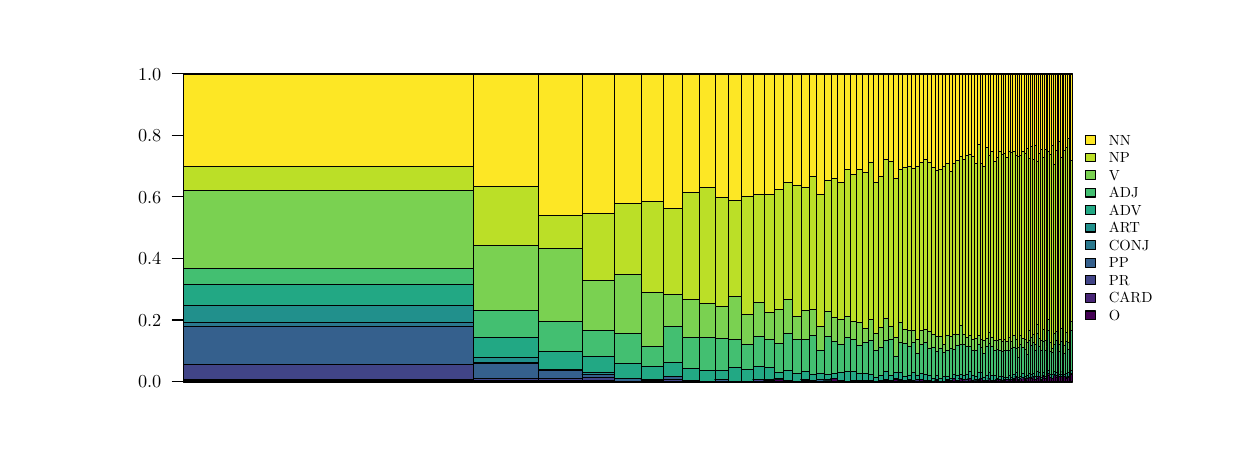
\begin{tikzpicture}[x=1pt,y=1pt]
\definecolor{fillColor}{RGB}{255,255,255}
\path[use as bounding box,fill=fillColor,fill opacity=0.00] (0,0) rectangle (433.62,144.54);
\begin{scope}
\path[clip] (  0.00,  0.00) rectangle (433.62,144.54);
\definecolor{drawColor}{RGB}{0,0,0}
\definecolor{fillColor}{RGB}{68,1,84}

\path[draw=drawColor,line width= 0.1pt,line join=round,line cap=round,fill=fillColor] ( 56.23, 16.63) rectangle (160.94, 17.14);
\definecolor{fillColor}{RGB}{72,37,118}

\path[draw=drawColor,line width= 0.1pt,line join=round,line cap=round,fill=fillColor] ( 56.23, 17.14) rectangle (160.94, 17.66);
\definecolor{fillColor}{RGB}{65,68,135}

\path[draw=drawColor,line width= 0.1pt,line join=round,line cap=round,fill=fillColor] ( 56.23, 17.66) rectangle (160.94, 22.79);
\definecolor{fillColor}{RGB}{53,96,141}

\path[draw=drawColor,line width= 0.1pt,line join=round,line cap=round,fill=fillColor] ( 56.23, 22.79) rectangle (160.94, 36.63);
\definecolor{fillColor}{RGB}{42,120,142}

\path[draw=drawColor,line width= 0.1pt,line join=round,line cap=round,fill=fillColor] ( 56.23, 36.63) rectangle (160.94, 38.17);
\definecolor{fillColor}{RGB}{33,144,140}

\path[draw=drawColor,line width= 0.1pt,line join=round,line cap=round,fill=fillColor] ( 56.23, 38.17) rectangle (160.94, 44.32);
\definecolor{fillColor}{RGB}{34,168,132}

\path[draw=drawColor,line width= 0.1pt,line join=round,line cap=round,fill=fillColor] ( 56.23, 44.32) rectangle (160.94, 52.01);
\definecolor{fillColor}{RGB}{67,191,113}

\path[draw=drawColor,line width= 0.1pt,line join=round,line cap=round,fill=fillColor] ( 56.23, 52.01) rectangle (160.94, 57.66);
\definecolor{fillColor}{RGB}{122,209,81}

\path[draw=drawColor,line width= 0.1pt,line join=round,line cap=round,fill=fillColor] ( 56.23, 57.66) rectangle (160.94, 85.86);
\definecolor{fillColor}{RGB}{187,223,39}

\path[draw=drawColor,line width= 0.1pt,line join=round,line cap=round,fill=fillColor] ( 56.23, 85.86) rectangle (160.94, 94.58);
\definecolor{fillColor}{RGB}{253,231,37}

\path[draw=drawColor,line width= 0.1pt,line join=round,line cap=round,fill=fillColor] ( 56.23, 94.58) rectangle (160.94,127.91);
\definecolor{fillColor}{RGB}{68,1,84}

\path[draw=drawColor,line width= 0.1pt,line join=round,line cap=round,fill=fillColor] (160.94, 16.63) rectangle (184.58, 17.08);
\definecolor{fillColor}{RGB}{72,37,118}

\path[draw=drawColor,line width= 0.1pt,line join=round,line cap=round,fill=fillColor] (160.94, 17.08) rectangle (184.58, 17.08);
\definecolor{fillColor}{RGB}{65,68,135}

\path[draw=drawColor,line width= 0.1pt,line join=round,line cap=round,fill=fillColor] (160.94, 17.08) rectangle (184.58, 17.96);
\definecolor{fillColor}{RGB}{53,96,141}

\path[draw=drawColor,line width= 0.1pt,line join=round,line cap=round,fill=fillColor] (160.94, 17.96) rectangle (184.58, 23.28);
\definecolor{fillColor}{RGB}{42,120,142}

\path[draw=drawColor,line width= 0.1pt,line join=round,line cap=round,fill=fillColor] (160.94, 23.28) rectangle (184.58, 23.73);
\definecolor{fillColor}{RGB}{33,144,140}

\path[draw=drawColor,line width= 0.1pt,line join=round,line cap=round,fill=fillColor] (160.94, 23.73) rectangle (184.58, 25.50);
\definecolor{fillColor}{RGB}{34,168,132}

\path[draw=drawColor,line width= 0.1pt,line join=round,line cap=round,fill=fillColor] (160.94, 25.50) rectangle (184.58, 32.59);
\definecolor{fillColor}{RGB}{67,191,113}

\path[draw=drawColor,line width= 0.1pt,line join=round,line cap=round,fill=fillColor] (160.94, 32.59) rectangle (184.58, 42.35);
\definecolor{fillColor}{RGB}{122,209,81}

\path[draw=drawColor,line width= 0.1pt,line join=round,line cap=round,fill=fillColor] (160.94, 42.35) rectangle (184.58, 65.84);
\definecolor{fillColor}{RGB}{187,223,39}

\path[draw=drawColor,line width= 0.1pt,line join=round,line cap=round,fill=fillColor] (160.94, 65.84) rectangle (184.58, 87.12);
\definecolor{fillColor}{RGB}{253,231,37}

\path[draw=drawColor,line width= 0.1pt,line join=round,line cap=round,fill=fillColor] (160.94, 87.12) rectangle (184.58,127.91);
\definecolor{fillColor}{RGB}{68,1,84}

\path[draw=drawColor,line width= 0.1pt,line join=round,line cap=round,fill=fillColor] (184.58, 16.63) rectangle (200.25, 16.63);
\definecolor{fillColor}{RGB}{72,37,118}

\path[draw=drawColor,line width= 0.1pt,line join=round,line cap=round,fill=fillColor] (184.58, 16.63) rectangle (200.25, 17.04);
\definecolor{fillColor}{RGB}{65,68,135}

\path[draw=drawColor,line width= 0.1pt,line join=round,line cap=round,fill=fillColor] (184.58, 17.04) rectangle (200.25, 17.87);
\definecolor{fillColor}{RGB}{53,96,141}

\path[draw=drawColor,line width= 0.1pt,line join=round,line cap=round,fill=fillColor] (184.58, 17.87) rectangle (200.25, 20.75);
\definecolor{fillColor}{RGB}{42,120,142}

\path[draw=drawColor,line width= 0.1pt,line join=round,line cap=round,fill=fillColor] (184.58, 20.75) rectangle (200.25, 21.17);
\definecolor{fillColor}{RGB}{33,144,140}

\path[draw=drawColor,line width= 0.1pt,line join=round,line cap=round,fill=fillColor] (184.58, 21.17) rectangle (200.25, 21.17);
\definecolor{fillColor}{RGB}{34,168,132}

\path[draw=drawColor,line width= 0.1pt,line join=round,line cap=round,fill=fillColor] (184.58, 21.17) rectangle (200.25, 27.76);
\definecolor{fillColor}{RGB}{67,191,113}

\path[draw=drawColor,line width= 0.1pt,line join=round,line cap=round,fill=fillColor] (184.58, 27.76) rectangle (200.25, 38.48);
\definecolor{fillColor}{RGB}{122,209,81}

\path[draw=drawColor,line width= 0.1pt,line join=round,line cap=round,fill=fillColor] (184.58, 38.48) rectangle (200.25, 64.85);
\definecolor{fillColor}{RGB}{187,223,39}

\path[draw=drawColor,line width= 0.1pt,line join=round,line cap=round,fill=fillColor] (184.58, 64.85) rectangle (200.25, 76.80);
\definecolor{fillColor}{RGB}{253,231,37}

\path[draw=drawColor,line width= 0.1pt,line join=round,line cap=round,fill=fillColor] (184.58, 76.80) rectangle (200.25,127.91);
\definecolor{fillColor}{RGB}{68,1,84}

\path[draw=drawColor,line width= 0.1pt,line join=round,line cap=round,fill=fillColor] (200.25, 16.63) rectangle (212.07, 17.02);
\definecolor{fillColor}{RGB}{72,37,118}

\path[draw=drawColor,line width= 0.1pt,line join=round,line cap=round,fill=fillColor] (200.25, 17.02) rectangle (212.07, 17.02);
\definecolor{fillColor}{RGB}{65,68,135}

\path[draw=drawColor,line width= 0.1pt,line join=round,line cap=round,fill=fillColor] (200.25, 17.02) rectangle (212.07, 18.18);
\definecolor{fillColor}{RGB}{53,96,141}

\path[draw=drawColor,line width= 0.1pt,line join=round,line cap=round,fill=fillColor] (200.25, 18.18) rectangle (212.07, 19.35);
\definecolor{fillColor}{RGB}{42,120,142}

\path[draw=drawColor,line width= 0.1pt,line join=round,line cap=round,fill=fillColor] (200.25, 19.35) rectangle (212.07, 19.35);
\definecolor{fillColor}{RGB}{33,144,140}

\path[draw=drawColor,line width= 0.1pt,line join=round,line cap=round,fill=fillColor] (200.25, 19.35) rectangle (212.07, 20.12);
\definecolor{fillColor}{RGB}{34,168,132}

\path[draw=drawColor,line width= 0.1pt,line join=round,line cap=round,fill=fillColor] (200.25, 20.12) rectangle (212.07, 25.94);
\definecolor{fillColor}{RGB}{67,191,113}

\path[draw=drawColor,line width= 0.1pt,line join=round,line cap=round,fill=fillColor] (200.25, 25.94) rectangle (212.07, 35.24);
\definecolor{fillColor}{RGB}{122,209,81}

\path[draw=drawColor,line width= 0.1pt,line join=round,line cap=round,fill=fillColor] (200.25, 35.24) rectangle (212.07, 53.47);
\definecolor{fillColor}{RGB}{187,223,39}

\path[draw=drawColor,line width= 0.1pt,line join=round,line cap=round,fill=fillColor] (200.25, 53.47) rectangle (212.07, 77.50);
\definecolor{fillColor}{RGB}{253,231,37}

\path[draw=drawColor,line width= 0.1pt,line join=round,line cap=round,fill=fillColor] (200.25, 77.50) rectangle (212.07,127.91);
\definecolor{fillColor}{RGB}{68,1,84}

\path[draw=drawColor,line width= 0.1pt,line join=round,line cap=round,fill=fillColor] (212.07, 16.63) rectangle (221.61, 16.63);
\definecolor{fillColor}{RGB}{72,37,118}

\path[draw=drawColor,line width= 0.1pt,line join=round,line cap=round,fill=fillColor] (212.07, 16.63) rectangle (221.61, 16.63);
\definecolor{fillColor}{RGB}{65,68,135}

\path[draw=drawColor,line width= 0.1pt,line join=round,line cap=round,fill=fillColor] (212.07, 16.63) rectangle (221.61, 16.63);
\definecolor{fillColor}{RGB}{53,96,141}

\path[draw=drawColor,line width= 0.1pt,line join=round,line cap=round,fill=fillColor] (212.07, 16.63) rectangle (221.61, 17.74);
\definecolor{fillColor}{RGB}{42,120,142}

\path[draw=drawColor,line width= 0.1pt,line join=round,line cap=round,fill=fillColor] (212.07, 17.74) rectangle (221.61, 17.74);
\definecolor{fillColor}{RGB}{33,144,140}

\path[draw=drawColor,line width= 0.1pt,line join=round,line cap=round,fill=fillColor] (212.07, 17.74) rectangle (221.61, 17.74);
\definecolor{fillColor}{RGB}{34,168,132}

\path[draw=drawColor,line width= 0.1pt,line join=round,line cap=round,fill=fillColor] (212.07, 17.74) rectangle (221.61, 23.31);
\definecolor{fillColor}{RGB}{67,191,113}

\path[draw=drawColor,line width= 0.1pt,line join=round,line cap=round,fill=fillColor] (212.07, 23.31) rectangle (221.61, 34.07);
\definecolor{fillColor}{RGB}{122,209,81}

\path[draw=drawColor,line width= 0.1pt,line join=round,line cap=round,fill=fillColor] (212.07, 34.07) rectangle (221.61, 55.58);
\definecolor{fillColor}{RGB}{187,223,39}

\path[draw=drawColor,line width= 0.1pt,line join=round,line cap=round,fill=fillColor] (212.07, 55.58) rectangle (221.61, 81.17);
\definecolor{fillColor}{RGB}{253,231,37}

\path[draw=drawColor,line width= 0.1pt,line join=round,line cap=round,fill=fillColor] (212.07, 81.17) rectangle (221.61,127.91);
\definecolor{fillColor}{RGB}{68,1,84}

\path[draw=drawColor,line width= 0.1pt,line join=round,line cap=round,fill=fillColor] (221.61, 16.63) rectangle (229.64, 16.63);
\definecolor{fillColor}{RGB}{72,37,118}

\path[draw=drawColor,line width= 0.1pt,line join=round,line cap=round,fill=fillColor] (221.61, 16.63) rectangle (229.64, 16.63);
\definecolor{fillColor}{RGB}{65,68,135}

\path[draw=drawColor,line width= 0.1pt,line join=round,line cap=round,fill=fillColor] (221.61, 16.63) rectangle (229.64, 17.34);
\definecolor{fillColor}{RGB}{53,96,141}

\path[draw=drawColor,line width= 0.1pt,line join=round,line cap=round,fill=fillColor] (221.61, 17.34) rectangle (229.64, 17.70);
\definecolor{fillColor}{RGB}{42,120,142}

\path[draw=drawColor,line width= 0.1pt,line join=round,line cap=round,fill=fillColor] (221.61, 17.70) rectangle (229.64, 17.70);
\definecolor{fillColor}{RGB}{33,144,140}

\path[draw=drawColor,line width= 0.1pt,line join=round,line cap=round,fill=fillColor] (221.61, 17.70) rectangle (229.64, 17.70);
\definecolor{fillColor}{RGB}{34,168,132}

\path[draw=drawColor,line width= 0.1pt,line join=round,line cap=round,fill=fillColor] (221.61, 17.70) rectangle (229.64, 22.32);
\definecolor{fillColor}{RGB}{67,191,113}

\path[draw=drawColor,line width= 0.1pt,line join=round,line cap=round,fill=fillColor] (221.61, 22.32) rectangle (229.64, 29.43);
\definecolor{fillColor}{RGB}{122,209,81}

\path[draw=drawColor,line width= 0.1pt,line join=round,line cap=round,fill=fillColor] (221.61, 29.43) rectangle (229.64, 48.98);
\definecolor{fillColor}{RGB}{187,223,39}

\path[draw=drawColor,line width= 0.1pt,line join=round,line cap=round,fill=fillColor] (221.61, 48.98) rectangle (229.64, 81.69);
\definecolor{fillColor}{RGB}{253,231,37}

\path[draw=drawColor,line width= 0.1pt,line join=round,line cap=round,fill=fillColor] (221.61, 81.69) rectangle (229.64,127.91);
\definecolor{fillColor}{RGB}{68,1,84}

\path[draw=drawColor,line width= 0.1pt,line join=round,line cap=round,fill=fillColor] (229.64, 16.63) rectangle (236.61, 16.63);
\definecolor{fillColor}{RGB}{72,37,118}

\path[draw=drawColor,line width= 0.1pt,line join=round,line cap=round,fill=fillColor] (229.64, 16.63) rectangle (236.61, 16.98);
\definecolor{fillColor}{RGB}{65,68,135}

\path[draw=drawColor,line width= 0.1pt,line join=round,line cap=round,fill=fillColor] (229.64, 16.98) rectangle (236.61, 17.66);
\definecolor{fillColor}{RGB}{53,96,141}

\path[draw=drawColor,line width= 0.1pt,line join=round,line cap=round,fill=fillColor] (229.64, 17.66) rectangle (236.61, 18.69);
\definecolor{fillColor}{RGB}{42,120,142}

\path[draw=drawColor,line width= 0.1pt,line join=round,line cap=round,fill=fillColor] (229.64, 18.69) rectangle (236.61, 18.69);
\definecolor{fillColor}{RGB}{33,144,140}

\path[draw=drawColor,line width= 0.1pt,line join=round,line cap=round,fill=fillColor] (229.64, 18.69) rectangle (236.61, 18.69);
\definecolor{fillColor}{RGB}{34,168,132}

\path[draw=drawColor,line width= 0.1pt,line join=round,line cap=round,fill=fillColor] (229.64, 18.69) rectangle (236.61, 23.50);
\definecolor{fillColor}{RGB}{67,191,113}

\path[draw=drawColor,line width= 0.1pt,line join=round,line cap=round,fill=fillColor] (229.64, 23.50) rectangle (236.61, 36.55);
\definecolor{fillColor}{RGB}{122,209,81}

\path[draw=drawColor,line width= 0.1pt,line join=round,line cap=round,fill=fillColor] (229.64, 36.55) rectangle (236.61, 48.23);
\definecolor{fillColor}{RGB}{187,223,39}

\path[draw=drawColor,line width= 0.1pt,line join=round,line cap=round,fill=fillColor] (229.64, 48.23) rectangle (236.61, 79.48);
\definecolor{fillColor}{RGB}{253,231,37}

\path[draw=drawColor,line width= 0.1pt,line join=round,line cap=round,fill=fillColor] (229.64, 79.48) rectangle (236.61,127.91);
\definecolor{fillColor}{RGB}{68,1,84}

\path[draw=drawColor,line width= 0.1pt,line join=round,line cap=round,fill=fillColor] (236.61, 16.63) rectangle (242.75, 16.63);
\definecolor{fillColor}{RGB}{72,37,118}

\path[draw=drawColor,line width= 0.1pt,line join=round,line cap=round,fill=fillColor] (236.61, 16.63) rectangle (242.75, 16.63);
\definecolor{fillColor}{RGB}{65,68,135}

\path[draw=drawColor,line width= 0.1pt,line join=round,line cap=round,fill=fillColor] (236.61, 16.63) rectangle (242.75, 16.63);
\definecolor{fillColor}{RGB}{53,96,141}

\path[draw=drawColor,line width= 0.1pt,line join=round,line cap=round,fill=fillColor] (236.61, 16.63) rectangle (242.75, 16.96);
\definecolor{fillColor}{RGB}{42,120,142}

\path[draw=drawColor,line width= 0.1pt,line join=round,line cap=round,fill=fillColor] (236.61, 16.96) rectangle (242.75, 17.30);
\definecolor{fillColor}{RGB}{33,144,140}

\path[draw=drawColor,line width= 0.1pt,line join=round,line cap=round,fill=fillColor] (236.61, 17.30) rectangle (242.75, 17.30);
\definecolor{fillColor}{RGB}{34,168,132}

\path[draw=drawColor,line width= 0.1pt,line join=round,line cap=round,fill=fillColor] (236.61, 17.30) rectangle (242.75, 21.61);
\definecolor{fillColor}{RGB}{67,191,113}

\path[draw=drawColor,line width= 0.1pt,line join=round,line cap=round,fill=fillColor] (236.61, 21.61) rectangle (242.75, 32.58);
\definecolor{fillColor}{RGB}{122,209,81}

\path[draw=drawColor,line width= 0.1pt,line join=round,line cap=round,fill=fillColor] (236.61, 32.58) rectangle (242.75, 46.53);
\definecolor{fillColor}{RGB}{187,223,39}

\path[draw=drawColor,line width= 0.1pt,line join=round,line cap=round,fill=fillColor] (236.61, 46.53) rectangle (242.75, 85.06);
\definecolor{fillColor}{RGB}{253,231,37}

\path[draw=drawColor,line width= 0.1pt,line join=round,line cap=round,fill=fillColor] (236.61, 85.06) rectangle (242.75,127.91);
\definecolor{fillColor}{RGB}{68,1,84}

\path[draw=drawColor,line width= 0.1pt,line join=round,line cap=round,fill=fillColor] (242.75, 16.63) rectangle (248.28, 16.63);
\definecolor{fillColor}{RGB}{72,37,118}

\path[draw=drawColor,line width= 0.1pt,line join=round,line cap=round,fill=fillColor] (242.75, 16.63) rectangle (248.28, 16.63);
\definecolor{fillColor}{RGB}{65,68,135}

\path[draw=drawColor,line width= 0.1pt,line join=round,line cap=round,fill=fillColor] (242.75, 16.63) rectangle (248.28, 16.63);
\definecolor{fillColor}{RGB}{53,96,141}

\path[draw=drawColor,line width= 0.1pt,line join=round,line cap=round,fill=fillColor] (242.75, 16.63) rectangle (248.28, 16.95);
\definecolor{fillColor}{RGB}{42,120,142}

\path[draw=drawColor,line width= 0.1pt,line join=round,line cap=round,fill=fillColor] (242.75, 16.95) rectangle (248.28, 16.95);
\definecolor{fillColor}{RGB}{33,144,140}

\path[draw=drawColor,line width= 0.1pt,line join=round,line cap=round,fill=fillColor] (242.75, 16.95) rectangle (248.28, 16.95);
\definecolor{fillColor}{RGB}{34,168,132}

\path[draw=drawColor,line width= 0.1pt,line join=round,line cap=round,fill=fillColor] (242.75, 16.95) rectangle (248.28, 20.81);
\definecolor{fillColor}{RGB}{67,191,113}

\path[draw=drawColor,line width= 0.1pt,line join=round,line cap=round,fill=fillColor] (242.75, 20.81) rectangle (248.28, 32.71);
\definecolor{fillColor}{RGB}{122,209,81}

\path[draw=drawColor,line width= 0.1pt,line join=round,line cap=round,fill=fillColor] (242.75, 32.71) rectangle (248.28, 44.93);
\definecolor{fillColor}{RGB}{187,223,39}

\path[draw=drawColor,line width= 0.1pt,line join=round,line cap=round,fill=fillColor] (242.75, 44.93) rectangle (248.28, 87.06);
\definecolor{fillColor}{RGB}{253,231,37}

\path[draw=drawColor,line width= 0.1pt,line join=round,line cap=round,fill=fillColor] (242.75, 87.06) rectangle (248.28,127.91);
\definecolor{fillColor}{RGB}{68,1,84}

\path[draw=drawColor,line width= 0.1pt,line join=round,line cap=round,fill=fillColor] (248.28, 16.63) rectangle (253.28, 16.63);
\definecolor{fillColor}{RGB}{72,37,118}

\path[draw=drawColor,line width= 0.1pt,line join=round,line cap=round,fill=fillColor] (248.28, 16.63) rectangle (253.28, 16.63);
\definecolor{fillColor}{RGB}{65,68,135}

\path[draw=drawColor,line width= 0.1pt,line join=round,line cap=round,fill=fillColor] (248.28, 16.63) rectangle (253.28, 16.94);
\definecolor{fillColor}{RGB}{53,96,141}

\path[draw=drawColor,line width= 0.1pt,line join=round,line cap=round,fill=fillColor] (248.28, 16.94) rectangle (253.28, 17.57);
\definecolor{fillColor}{RGB}{42,120,142}

\path[draw=drawColor,line width= 0.1pt,line join=round,line cap=round,fill=fillColor] (248.28, 17.57) rectangle (253.28, 17.57);
\definecolor{fillColor}{RGB}{33,144,140}

\path[draw=drawColor,line width= 0.1pt,line join=round,line cap=round,fill=fillColor] (248.28, 17.57) rectangle (253.28, 17.57);
\definecolor{fillColor}{RGB}{34,168,132}

\path[draw=drawColor,line width= 0.1pt,line join=round,line cap=round,fill=fillColor] (248.28, 17.57) rectangle (253.28, 20.68);
\definecolor{fillColor}{RGB}{67,191,113}

\path[draw=drawColor,line width= 0.1pt,line join=round,line cap=round,fill=fillColor] (248.28, 20.68) rectangle (253.28, 32.53);
\definecolor{fillColor}{RGB}{122,209,81}

\path[draw=drawColor,line width= 0.1pt,line join=round,line cap=round,fill=fillColor] (248.28, 32.53) rectangle (253.28, 43.75);
\definecolor{fillColor}{RGB}{187,223,39}

\path[draw=drawColor,line width= 0.1pt,line join=round,line cap=round,fill=fillColor] (248.28, 43.75) rectangle (253.28, 83.34);
\definecolor{fillColor}{RGB}{253,231,37}

\path[draw=drawColor,line width= 0.1pt,line join=round,line cap=round,fill=fillColor] (248.28, 83.34) rectangle (253.28,127.91);
\definecolor{fillColor}{RGB}{68,1,84}

\path[draw=drawColor,line width= 0.1pt,line join=round,line cap=round,fill=fillColor] (253.28, 16.63) rectangle (257.84, 16.63);
\definecolor{fillColor}{RGB}{72,37,118}

\path[draw=drawColor,line width= 0.1pt,line join=round,line cap=round,fill=fillColor] (253.28, 16.63) rectangle (257.84, 16.63);
\definecolor{fillColor}{RGB}{65,68,135}

\path[draw=drawColor,line width= 0.1pt,line join=round,line cap=round,fill=fillColor] (253.28, 16.63) rectangle (257.84, 16.63);
\definecolor{fillColor}{RGB}{53,96,141}

\path[draw=drawColor,line width= 0.1pt,line join=round,line cap=round,fill=fillColor] (253.28, 16.63) rectangle (257.84, 16.63);
\definecolor{fillColor}{RGB}{42,120,142}

\path[draw=drawColor,line width= 0.1pt,line join=round,line cap=round,fill=fillColor] (253.28, 16.63) rectangle (257.84, 16.63);
\definecolor{fillColor}{RGB}{33,144,140}

\path[draw=drawColor,line width= 0.1pt,line join=round,line cap=round,fill=fillColor] (253.28, 16.63) rectangle (257.84, 16.63);
\definecolor{fillColor}{RGB}{34,168,132}

\path[draw=drawColor,line width= 0.1pt,line join=round,line cap=round,fill=fillColor] (253.28, 16.63) rectangle (257.84, 21.80);
\definecolor{fillColor}{RGB}{67,191,113}

\path[draw=drawColor,line width= 0.1pt,line join=round,line cap=round,fill=fillColor] (253.28, 21.80) rectangle (257.84, 32.14);
\definecolor{fillColor}{RGB}{122,209,81}

\path[draw=drawColor,line width= 0.1pt,line join=round,line cap=round,fill=fillColor] (253.28, 32.14) rectangle (257.84, 47.64);
\definecolor{fillColor}{RGB}{187,223,39}

\path[draw=drawColor,line width= 0.1pt,line join=round,line cap=round,fill=fillColor] (253.28, 47.64) rectangle (257.84, 82.30);
\definecolor{fillColor}{RGB}{253,231,37}

\path[draw=drawColor,line width= 0.1pt,line join=round,line cap=round,fill=fillColor] (253.28, 82.30) rectangle (257.84,127.91);
\definecolor{fillColor}{RGB}{68,1,84}

\path[draw=drawColor,line width= 0.1pt,line join=round,line cap=round,fill=fillColor] (257.84, 16.63) rectangle (262.05, 16.63);
\definecolor{fillColor}{RGB}{72,37,118}

\path[draw=drawColor,line width= 0.1pt,line join=round,line cap=round,fill=fillColor] (257.84, 16.63) rectangle (262.05, 16.63);
\definecolor{fillColor}{RGB}{65,68,135}

\path[draw=drawColor,line width= 0.1pt,line join=round,line cap=round,fill=fillColor] (257.84, 16.63) rectangle (262.05, 16.63);
\definecolor{fillColor}{RGB}{53,96,141}

\path[draw=drawColor,line width= 0.1pt,line join=round,line cap=round,fill=fillColor] (257.84, 16.63) rectangle (262.05, 16.63);
\definecolor{fillColor}{RGB}{42,120,142}

\path[draw=drawColor,line width= 0.1pt,line join=round,line cap=round,fill=fillColor] (257.84, 16.63) rectangle (262.05, 16.63);
\definecolor{fillColor}{RGB}{33,144,140}

\path[draw=drawColor,line width= 0.1pt,line join=round,line cap=round,fill=fillColor] (257.84, 16.63) rectangle (262.05, 16.63);
\definecolor{fillColor}{RGB}{34,168,132}

\path[draw=drawColor,line width= 0.1pt,line join=round,line cap=round,fill=fillColor] (257.84, 16.63) rectangle (262.05, 21.07);
\definecolor{fillColor}{RGB}{67,191,113}

\path[draw=drawColor,line width= 0.1pt,line join=round,line cap=round,fill=fillColor] (257.84, 21.07) rectangle (262.05, 30.25);
\definecolor{fillColor}{RGB}{122,209,81}

\path[draw=drawColor,line width= 0.1pt,line join=round,line cap=round,fill=fillColor] (257.84, 30.25) rectangle (262.05, 40.90);
\definecolor{fillColor}{RGB}{187,223,39}

\path[draw=drawColor,line width= 0.1pt,line join=round,line cap=round,fill=fillColor] (257.84, 40.90) rectangle (262.05, 83.81);
\definecolor{fillColor}{RGB}{253,231,37}

\path[draw=drawColor,line width= 0.1pt,line join=round,line cap=round,fill=fillColor] (257.84, 83.81) rectangle (262.05,127.91);
\definecolor{fillColor}{RGB}{68,1,84}

\path[draw=drawColor,line width= 0.1pt,line join=round,line cap=round,fill=fillColor] (262.05, 16.63) rectangle (265.97, 16.92);
\definecolor{fillColor}{RGB}{72,37,118}

\path[draw=drawColor,line width= 0.1pt,line join=round,line cap=round,fill=fillColor] (262.05, 16.92) rectangle (265.97, 16.92);
\definecolor{fillColor}{RGB}{65,68,135}

\path[draw=drawColor,line width= 0.1pt,line join=round,line cap=round,fill=fillColor] (262.05, 16.92) rectangle (265.97, 17.50);
\definecolor{fillColor}{RGB}{53,96,141}

\path[draw=drawColor,line width= 0.1pt,line join=round,line cap=round,fill=fillColor] (262.05, 17.50) rectangle (265.97, 17.50);
\definecolor{fillColor}{RGB}{42,120,142}

\path[draw=drawColor,line width= 0.1pt,line join=round,line cap=round,fill=fillColor] (262.05, 17.50) rectangle (265.97, 17.50);
\definecolor{fillColor}{RGB}{33,144,140}

\path[draw=drawColor,line width= 0.1pt,line join=round,line cap=round,fill=fillColor] (262.05, 17.50) rectangle (265.97, 17.50);
\definecolor{fillColor}{RGB}{34,168,132}

\path[draw=drawColor,line width= 0.1pt,line join=round,line cap=round,fill=fillColor] (262.05, 17.50) rectangle (265.97, 22.41);
\definecolor{fillColor}{RGB}{67,191,113}

\path[draw=drawColor,line width= 0.1pt,line join=round,line cap=round,fill=fillColor] (262.05, 22.41) rectangle (265.97, 33.11);
\definecolor{fillColor}{RGB}{122,209,81}

\path[draw=drawColor,line width= 0.1pt,line join=round,line cap=round,fill=fillColor] (262.05, 33.11) rectangle (265.97, 45.25);
\definecolor{fillColor}{RGB}{187,223,39}

\path[draw=drawColor,line width= 0.1pt,line join=round,line cap=round,fill=fillColor] (262.05, 45.25) rectangle (265.97, 84.26);
\definecolor{fillColor}{RGB}{253,231,37}

\path[draw=drawColor,line width= 0.1pt,line join=round,line cap=round,fill=fillColor] (262.05, 84.26) rectangle (265.97,127.91);
\definecolor{fillColor}{RGB}{68,1,84}

\path[draw=drawColor,line width= 0.1pt,line join=round,line cap=round,fill=fillColor] (265.97, 16.63) rectangle (269.62, 17.20);
\definecolor{fillColor}{RGB}{72,37,118}

\path[draw=drawColor,line width= 0.1pt,line join=round,line cap=round,fill=fillColor] (265.97, 17.20) rectangle (269.62, 17.20);
\definecolor{fillColor}{RGB}{65,68,135}

\path[draw=drawColor,line width= 0.1pt,line join=round,line cap=round,fill=fillColor] (265.97, 17.20) rectangle (269.62, 17.20);
\definecolor{fillColor}{RGB}{53,96,141}

\path[draw=drawColor,line width= 0.1pt,line join=round,line cap=round,fill=fillColor] (265.97, 17.20) rectangle (269.62, 17.48);
\definecolor{fillColor}{RGB}{42,120,142}

\path[draw=drawColor,line width= 0.1pt,line join=round,line cap=round,fill=fillColor] (265.97, 17.48) rectangle (269.62, 17.48);
\definecolor{fillColor}{RGB}{33,144,140}

\path[draw=drawColor,line width= 0.1pt,line join=round,line cap=round,fill=fillColor] (265.97, 17.48) rectangle (269.62, 17.48);
\definecolor{fillColor}{RGB}{34,168,132}

\path[draw=drawColor,line width= 0.1pt,line join=round,line cap=round,fill=fillColor] (265.97, 17.48) rectangle (269.62, 21.70);
\definecolor{fillColor}{RGB}{67,191,113}

\path[draw=drawColor,line width= 0.1pt,line join=round,line cap=round,fill=fillColor] (265.97, 21.70) rectangle (269.62, 32.13);
\definecolor{fillColor}{RGB}{122,209,81}

\path[draw=drawColor,line width= 0.1pt,line join=round,line cap=round,fill=fillColor] (265.97, 32.13) rectangle (269.62, 41.70);
\definecolor{fillColor}{RGB}{187,223,39}

\path[draw=drawColor,line width= 0.1pt,line join=round,line cap=round,fill=fillColor] (265.97, 41.70) rectangle (269.62, 84.52);
\definecolor{fillColor}{RGB}{253,231,37}

\path[draw=drawColor,line width= 0.1pt,line join=round,line cap=round,fill=fillColor] (265.97, 84.52) rectangle (269.62,127.91);
\definecolor{fillColor}{RGB}{68,1,84}

\path[draw=drawColor,line width= 0.1pt,line join=round,line cap=round,fill=fillColor] (269.62, 16.63) rectangle (273.04, 17.46);
\definecolor{fillColor}{RGB}{72,37,118}

\path[draw=drawColor,line width= 0.1pt,line join=round,line cap=round,fill=fillColor] (269.62, 17.46) rectangle (273.04, 17.46);
\definecolor{fillColor}{RGB}{65,68,135}

\path[draw=drawColor,line width= 0.1pt,line join=round,line cap=round,fill=fillColor] (269.62, 17.46) rectangle (273.04, 17.46);
\definecolor{fillColor}{RGB}{53,96,141}

\path[draw=drawColor,line width= 0.1pt,line join=round,line cap=round,fill=fillColor] (269.62, 17.46) rectangle (273.04, 17.74);
\definecolor{fillColor}{RGB}{42,120,142}

\path[draw=drawColor,line width= 0.1pt,line join=round,line cap=round,fill=fillColor] (269.62, 17.74) rectangle (273.04, 17.74);
\definecolor{fillColor}{RGB}{33,144,140}

\path[draw=drawColor,line width= 0.1pt,line join=round,line cap=round,fill=fillColor] (269.62, 17.74) rectangle (273.04, 18.01);
\definecolor{fillColor}{RGB}{34,168,132}

\path[draw=drawColor,line width= 0.1pt,line join=round,line cap=round,fill=fillColor] (269.62, 18.01) rectangle (273.04, 19.95);
\definecolor{fillColor}{RGB}{67,191,113}

\path[draw=drawColor,line width= 0.1pt,line join=round,line cap=round,fill=fillColor] (269.62, 19.95) rectangle (273.04, 30.44);
\definecolor{fillColor}{RGB}{122,209,81}

\path[draw=drawColor,line width= 0.1pt,line join=round,line cap=round,fill=fillColor] (269.62, 30.44) rectangle (273.04, 42.86);
\definecolor{fillColor}{RGB}{187,223,39}

\path[draw=drawColor,line width= 0.1pt,line join=round,line cap=round,fill=fillColor] (269.62, 42.86) rectangle (273.04, 86.21);
\definecolor{fillColor}{RGB}{253,231,37}

\path[draw=drawColor,line width= 0.1pt,line join=round,line cap=round,fill=fillColor] (269.62, 86.21) rectangle (273.04,127.91);
\definecolor{fillColor}{RGB}{68,1,84}

\path[draw=drawColor,line width= 0.1pt,line join=round,line cap=round,fill=fillColor] (273.04, 16.63) rectangle (276.27, 16.63);
\definecolor{fillColor}{RGB}{72,37,118}

\path[draw=drawColor,line width= 0.1pt,line join=round,line cap=round,fill=fillColor] (273.04, 16.63) rectangle (276.27, 16.63);
\definecolor{fillColor}{RGB}{65,68,135}

\path[draw=drawColor,line width= 0.1pt,line join=round,line cap=round,fill=fillColor] (273.04, 16.63) rectangle (276.27, 16.90);
\definecolor{fillColor}{RGB}{53,96,141}

\path[draw=drawColor,line width= 0.1pt,line join=round,line cap=round,fill=fillColor] (273.04, 16.90) rectangle (276.27, 17.17);
\definecolor{fillColor}{RGB}{42,120,142}

\path[draw=drawColor,line width= 0.1pt,line join=round,line cap=round,fill=fillColor] (273.04, 17.17) rectangle (276.27, 17.17);
\definecolor{fillColor}{RGB}{33,144,140}

\path[draw=drawColor,line width= 0.1pt,line join=round,line cap=round,fill=fillColor] (273.04, 17.17) rectangle (276.27, 17.17);
\definecolor{fillColor}{RGB}{34,168,132}

\path[draw=drawColor,line width= 0.1pt,line join=round,line cap=round,fill=fillColor] (273.04, 17.17) rectangle (276.27, 20.94);
\definecolor{fillColor}{RGB}{67,191,113}

\path[draw=drawColor,line width= 0.1pt,line join=round,line cap=round,fill=fillColor] (273.04, 20.94) rectangle (276.27, 34.15);
\definecolor{fillColor}{RGB}{122,209,81}

\path[draw=drawColor,line width= 0.1pt,line join=round,line cap=round,fill=fillColor] (273.04, 34.15) rectangle (276.27, 46.54);
\definecolor{fillColor}{RGB}{187,223,39}

\path[draw=drawColor,line width= 0.1pt,line join=round,line cap=round,fill=fillColor] (273.04, 46.54) rectangle (276.27, 88.84);
\definecolor{fillColor}{RGB}{253,231,37}

\path[draw=drawColor,line width= 0.1pt,line join=round,line cap=round,fill=fillColor] (273.04, 88.84) rectangle (276.27,127.91);
\definecolor{fillColor}{RGB}{68,1,84}

\path[draw=drawColor,line width= 0.1pt,line join=round,line cap=round,fill=fillColor] (276.27, 16.63) rectangle (279.33, 16.90);
\definecolor{fillColor}{RGB}{72,37,118}

\path[draw=drawColor,line width= 0.1pt,line join=round,line cap=round,fill=fillColor] (276.27, 16.90) rectangle (279.33, 16.90);
\definecolor{fillColor}{RGB}{65,68,135}

\path[draw=drawColor,line width= 0.1pt,line join=round,line cap=round,fill=fillColor] (276.27, 16.90) rectangle (279.33, 16.90);
\definecolor{fillColor}{RGB}{53,96,141}

\path[draw=drawColor,line width= 0.1pt,line join=round,line cap=round,fill=fillColor] (276.27, 16.90) rectangle (279.33, 16.90);
\definecolor{fillColor}{RGB}{42,120,142}

\path[draw=drawColor,line width= 0.1pt,line join=round,line cap=round,fill=fillColor] (276.27, 16.90) rectangle (279.33, 16.90);
\definecolor{fillColor}{RGB}{33,144,140}

\path[draw=drawColor,line width= 0.1pt,line join=round,line cap=round,fill=fillColor] (276.27, 16.90) rectangle (279.33, 16.90);
\definecolor{fillColor}{RGB}{34,168,132}

\path[draw=drawColor,line width= 0.1pt,line join=round,line cap=round,fill=fillColor] (276.27, 16.90) rectangle (279.33, 19.82);
\definecolor{fillColor}{RGB}{67,191,113}

\path[draw=drawColor,line width= 0.1pt,line join=round,line cap=round,fill=fillColor] (276.27, 19.82) rectangle (279.33, 32.04);
\definecolor{fillColor}{RGB}{122,209,81}

\path[draw=drawColor,line width= 0.1pt,line join=round,line cap=round,fill=fillColor] (276.27, 32.04) rectangle (279.33, 40.27);
\definecolor{fillColor}{RGB}{187,223,39}

\path[draw=drawColor,line width= 0.1pt,line join=round,line cap=round,fill=fillColor] (276.27, 40.27) rectangle (279.33, 87.81);
\definecolor{fillColor}{RGB}{253,231,37}

\path[draw=drawColor,line width= 0.1pt,line join=round,line cap=round,fill=fillColor] (276.27, 87.81) rectangle (279.33,127.91);
\definecolor{fillColor}{RGB}{68,1,84}

\path[draw=drawColor,line width= 0.1pt,line join=round,line cap=round,fill=fillColor] (279.33, 16.63) rectangle (282.25, 17.15);
\definecolor{fillColor}{RGB}{72,37,118}

\path[draw=drawColor,line width= 0.1pt,line join=round,line cap=round,fill=fillColor] (279.33, 17.15) rectangle (282.25, 17.41);
\definecolor{fillColor}{RGB}{65,68,135}

\path[draw=drawColor,line width= 0.1pt,line join=round,line cap=round,fill=fillColor] (279.33, 17.41) rectangle (282.25, 17.41);
\definecolor{fillColor}{RGB}{53,96,141}

\path[draw=drawColor,line width= 0.1pt,line join=round,line cap=round,fill=fillColor] (279.33, 17.41) rectangle (282.25, 17.67);
\definecolor{fillColor}{RGB}{42,120,142}

\path[draw=drawColor,line width= 0.1pt,line join=round,line cap=round,fill=fillColor] (279.33, 17.67) rectangle (282.25, 17.67);
\definecolor{fillColor}{RGB}{33,144,140}

\path[draw=drawColor,line width= 0.1pt,line join=round,line cap=round,fill=fillColor] (279.33, 17.67) rectangle (282.25, 17.67);
\definecolor{fillColor}{RGB}{34,168,132}

\path[draw=drawColor,line width= 0.1pt,line join=round,line cap=round,fill=fillColor] (279.33, 17.67) rectangle (282.25, 20.51);
\definecolor{fillColor}{RGB}{67,191,113}

\path[draw=drawColor,line width= 0.1pt,line join=round,line cap=round,fill=fillColor] (279.33, 20.51) rectangle (282.25, 31.90);
\definecolor{fillColor}{RGB}{122,209,81}

\path[draw=drawColor,line width= 0.1pt,line join=round,line cap=round,fill=fillColor] (279.33, 31.90) rectangle (282.25, 42.51);
\definecolor{fillColor}{RGB}{187,223,39}

\path[draw=drawColor,line width= 0.1pt,line join=round,line cap=round,fill=fillColor] (279.33, 42.51) rectangle (282.25, 87.02);
\definecolor{fillColor}{RGB}{253,231,37}

\path[draw=drawColor,line width= 0.1pt,line join=round,line cap=round,fill=fillColor] (279.33, 87.02) rectangle (282.25,127.91);
\definecolor{fillColor}{RGB}{68,1,84}

\path[draw=drawColor,line width= 0.1pt,line join=round,line cap=round,fill=fillColor] (282.25, 16.63) rectangle (285.03, 16.89);
\definecolor{fillColor}{RGB}{72,37,118}

\path[draw=drawColor,line width= 0.1pt,line join=round,line cap=round,fill=fillColor] (282.25, 16.89) rectangle (285.03, 17.14);
\definecolor{fillColor}{RGB}{65,68,135}

\path[draw=drawColor,line width= 0.1pt,line join=round,line cap=round,fill=fillColor] (282.25, 17.14) rectangle (285.03, 17.14);
\definecolor{fillColor}{RGB}{53,96,141}

\path[draw=drawColor,line width= 0.1pt,line join=round,line cap=round,fill=fillColor] (282.25, 17.14) rectangle (285.03, 17.14);
\definecolor{fillColor}{RGB}{42,120,142}

\path[draw=drawColor,line width= 0.1pt,line join=round,line cap=round,fill=fillColor] (282.25, 17.14) rectangle (285.03, 17.14);
\definecolor{fillColor}{RGB}{33,144,140}

\path[draw=drawColor,line width= 0.1pt,line join=round,line cap=round,fill=fillColor] (282.25, 17.14) rectangle (285.03, 17.14);
\definecolor{fillColor}{RGB}{34,168,132}

\path[draw=drawColor,line width= 0.1pt,line join=round,line cap=round,fill=fillColor] (282.25, 17.14) rectangle (285.03, 19.17);
\definecolor{fillColor}{RGB}{67,191,113}

\path[draw=drawColor,line width= 0.1pt,line join=round,line cap=round,fill=fillColor] (282.25, 19.17) rectangle (285.03, 33.40);
\definecolor{fillColor}{RGB}{122,209,81}

\path[draw=drawColor,line width= 0.1pt,line join=round,line cap=round,fill=fillColor] (282.25, 33.40) rectangle (285.03, 42.80);
\definecolor{fillColor}{RGB}{187,223,39}

\path[draw=drawColor,line width= 0.1pt,line join=round,line cap=round,fill=fillColor] (282.25, 42.80) rectangle (285.03, 91.07);
\definecolor{fillColor}{RGB}{253,231,37}

\path[draw=drawColor,line width= 0.1pt,line join=round,line cap=round,fill=fillColor] (282.25, 91.07) rectangle (285.03,127.91);
\definecolor{fillColor}{RGB}{68,1,84}

\path[draw=drawColor,line width= 0.1pt,line join=round,line cap=round,fill=fillColor] (285.03, 16.63) rectangle (287.68, 16.63);
\definecolor{fillColor}{RGB}{72,37,118}

\path[draw=drawColor,line width= 0.1pt,line join=round,line cap=round,fill=fillColor] (285.03, 16.63) rectangle (287.68, 16.88);
\definecolor{fillColor}{RGB}{65,68,135}

\path[draw=drawColor,line width= 0.1pt,line join=round,line cap=round,fill=fillColor] (285.03, 16.88) rectangle (287.68, 16.88);
\definecolor{fillColor}{RGB}{53,96,141}

\path[draw=drawColor,line width= 0.1pt,line join=round,line cap=round,fill=fillColor] (285.03, 16.88) rectangle (287.68, 17.38);
\definecolor{fillColor}{RGB}{42,120,142}

\path[draw=drawColor,line width= 0.1pt,line join=round,line cap=round,fill=fillColor] (285.03, 17.38) rectangle (287.68, 17.38);
\definecolor{fillColor}{RGB}{33,144,140}

\path[draw=drawColor,line width= 0.1pt,line join=round,line cap=round,fill=fillColor] (285.03, 17.38) rectangle (287.68, 17.38);
\definecolor{fillColor}{RGB}{34,168,132}

\path[draw=drawColor,line width= 0.1pt,line join=round,line cap=round,fill=fillColor] (285.03, 17.38) rectangle (287.68, 19.62);
\definecolor{fillColor}{RGB}{67,191,113}

\path[draw=drawColor,line width= 0.1pt,line join=round,line cap=round,fill=fillColor] (285.03, 19.62) rectangle (287.68, 28.08);
\definecolor{fillColor}{RGB}{122,209,81}

\path[draw=drawColor,line width= 0.1pt,line join=round,line cap=round,fill=fillColor] (285.03, 28.08) rectangle (287.68, 36.55);
\definecolor{fillColor}{RGB}{187,223,39}

\path[draw=drawColor,line width= 0.1pt,line join=round,line cap=round,fill=fillColor] (285.03, 36.55) rectangle (287.68, 84.34);
\definecolor{fillColor}{RGB}{253,231,37}

\path[draw=drawColor,line width= 0.1pt,line join=round,line cap=round,fill=fillColor] (285.03, 84.34) rectangle (287.68,127.91);
\definecolor{fillColor}{RGB}{68,1,84}

\path[draw=drawColor,line width= 0.1pt,line join=round,line cap=round,fill=fillColor] (287.68, 16.63) rectangle (290.23, 17.12);
\definecolor{fillColor}{RGB}{72,37,118}

\path[draw=drawColor,line width= 0.1pt,line join=round,line cap=round,fill=fillColor] (287.68, 17.12) rectangle (290.23, 17.12);
\definecolor{fillColor}{RGB}{65,68,135}

\path[draw=drawColor,line width= 0.1pt,line join=round,line cap=round,fill=fillColor] (287.68, 17.12) rectangle (290.23, 17.12);
\definecolor{fillColor}{RGB}{53,96,141}

\path[draw=drawColor,line width= 0.1pt,line join=round,line cap=round,fill=fillColor] (287.68, 17.12) rectangle (290.23, 17.36);
\definecolor{fillColor}{RGB}{42,120,142}

\path[draw=drawColor,line width= 0.1pt,line join=round,line cap=round,fill=fillColor] (287.68, 17.36) rectangle (290.23, 17.36);
\definecolor{fillColor}{RGB}{33,144,140}

\path[draw=drawColor,line width= 0.1pt,line join=round,line cap=round,fill=fillColor] (287.68, 17.36) rectangle (290.23, 17.36);
\definecolor{fillColor}{RGB}{34,168,132}

\path[draw=drawColor,line width= 0.1pt,line join=round,line cap=round,fill=fillColor] (287.68, 17.36) rectangle (290.23, 19.32);
\definecolor{fillColor}{RGB}{67,191,113}

\path[draw=drawColor,line width= 0.1pt,line join=round,line cap=round,fill=fillColor] (287.68, 19.32) rectangle (290.23, 33.23);
\definecolor{fillColor}{RGB}{122,209,81}

\path[draw=drawColor,line width= 0.1pt,line join=round,line cap=round,fill=fillColor] (287.68, 33.23) rectangle (290.23, 42.25);
\definecolor{fillColor}{RGB}{187,223,39}

\path[draw=drawColor,line width= 0.1pt,line join=round,line cap=round,fill=fillColor] (287.68, 42.25) rectangle (290.23, 89.35);
\definecolor{fillColor}{RGB}{253,231,37}

\path[draw=drawColor,line width= 0.1pt,line join=round,line cap=round,fill=fillColor] (287.68, 89.35) rectangle (290.23,127.91);
\definecolor{fillColor}{RGB}{68,1,84}

\path[draw=drawColor,line width= 0.1pt,line join=round,line cap=round,fill=fillColor] (290.23, 16.63) rectangle (292.67, 17.83);
\definecolor{fillColor}{RGB}{72,37,118}

\path[draw=drawColor,line width= 0.1pt,line join=round,line cap=round,fill=fillColor] (290.23, 17.83) rectangle (292.67, 17.83);
\definecolor{fillColor}{RGB}{65,68,135}

\path[draw=drawColor,line width= 0.1pt,line join=round,line cap=round,fill=fillColor] (290.23, 17.83) rectangle (292.67, 17.83);
\definecolor{fillColor}{RGB}{53,96,141}

\path[draw=drawColor,line width= 0.1pt,line join=round,line cap=round,fill=fillColor] (290.23, 17.83) rectangle (292.67, 17.83);
\definecolor{fillColor}{RGB}{42,120,142}

\path[draw=drawColor,line width= 0.1pt,line join=round,line cap=round,fill=fillColor] (290.23, 17.83) rectangle (292.67, 17.83);
\definecolor{fillColor}{RGB}{33,144,140}

\path[draw=drawColor,line width= 0.1pt,line join=round,line cap=round,fill=fillColor] (290.23, 17.83) rectangle (292.67, 17.83);
\definecolor{fillColor}{RGB}{34,168,132}

\path[draw=drawColor,line width= 0.1pt,line join=round,line cap=round,fill=fillColor] (290.23, 17.83) rectangle (292.67, 19.74);
\definecolor{fillColor}{RGB}{67,191,113}

\path[draw=drawColor,line width= 0.1pt,line join=round,line cap=round,fill=fillColor] (290.23, 19.74) rectangle (292.67, 31.23);
\definecolor{fillColor}{RGB}{122,209,81}

\path[draw=drawColor,line width= 0.1pt,line join=round,line cap=round,fill=fillColor] (290.23, 31.23) rectangle (292.67, 40.08);
\definecolor{fillColor}{RGB}{187,223,39}

\path[draw=drawColor,line width= 0.1pt,line join=round,line cap=round,fill=fillColor] (290.23, 40.08) rectangle (292.67, 90.10);
\definecolor{fillColor}{RGB}{253,231,37}

\path[draw=drawColor,line width= 0.1pt,line join=round,line cap=round,fill=fillColor] (290.23, 90.10) rectangle (292.67,127.91);
\definecolor{fillColor}{RGB}{68,1,84}

\path[draw=drawColor,line width= 0.1pt,line join=round,line cap=round,fill=fillColor] (292.67, 16.63) rectangle (295.01, 16.87);
\definecolor{fillColor}{RGB}{72,37,118}

\path[draw=drawColor,line width= 0.1pt,line join=round,line cap=round,fill=fillColor] (292.67, 16.87) rectangle (295.01, 16.87);
\definecolor{fillColor}{RGB}{65,68,135}

\path[draw=drawColor,line width= 0.1pt,line join=round,line cap=round,fill=fillColor] (292.67, 16.87) rectangle (295.01, 16.87);
\definecolor{fillColor}{RGB}{53,96,141}

\path[draw=drawColor,line width= 0.1pt,line join=round,line cap=round,fill=fillColor] (292.67, 16.87) rectangle (295.01, 17.10);
\definecolor{fillColor}{RGB}{42,120,142}

\path[draw=drawColor,line width= 0.1pt,line join=round,line cap=round,fill=fillColor] (292.67, 17.10) rectangle (295.01, 17.10);
\definecolor{fillColor}{RGB}{33,144,140}

\path[draw=drawColor,line width= 0.1pt,line join=round,line cap=round,fill=fillColor] (292.67, 17.10) rectangle (295.01, 17.10);
\definecolor{fillColor}{RGB}{34,168,132}

\path[draw=drawColor,line width= 0.1pt,line join=round,line cap=round,fill=fillColor] (292.67, 17.10) rectangle (295.01, 20.15);
\definecolor{fillColor}{RGB}{67,191,113}

\path[draw=drawColor,line width= 0.1pt,line join=round,line cap=round,fill=fillColor] (292.67, 20.15) rectangle (295.01, 30.25);
\definecolor{fillColor}{RGB}{122,209,81}

\path[draw=drawColor,line width= 0.1pt,line join=round,line cap=round,fill=fillColor] (292.67, 30.25) rectangle (295.01, 39.17);
\definecolor{fillColor}{RGB}{187,223,39}

\path[draw=drawColor,line width= 0.1pt,line join=round,line cap=round,fill=fillColor] (292.67, 39.17) rectangle (295.01, 88.70);
\definecolor{fillColor}{RGB}{253,231,37}

\path[draw=drawColor,line width= 0.1pt,line join=round,line cap=round,fill=fillColor] (292.67, 88.70) rectangle (295.01,127.91);
\definecolor{fillColor}{RGB}{68,1,84}

\path[draw=drawColor,line width= 0.1pt,line join=round,line cap=round,fill=fillColor] (295.01, 16.63) rectangle (297.27, 16.63);
\definecolor{fillColor}{RGB}{72,37,118}

\path[draw=drawColor,line width= 0.1pt,line join=round,line cap=round,fill=fillColor] (295.01, 16.63) rectangle (297.27, 16.63);
\definecolor{fillColor}{RGB}{65,68,135}

\path[draw=drawColor,line width= 0.1pt,line join=round,line cap=round,fill=fillColor] (295.01, 16.63) rectangle (297.27, 16.63);
\definecolor{fillColor}{RGB}{53,96,141}

\path[draw=drawColor,line width= 0.1pt,line join=round,line cap=round,fill=fillColor] (295.01, 16.63) rectangle (297.27, 16.86);
\definecolor{fillColor}{RGB}{42,120,142}

\path[draw=drawColor,line width= 0.1pt,line join=round,line cap=round,fill=fillColor] (295.01, 16.86) rectangle (297.27, 16.86);
\definecolor{fillColor}{RGB}{33,144,140}

\path[draw=drawColor,line width= 0.1pt,line join=round,line cap=round,fill=fillColor] (295.01, 16.86) rectangle (297.27, 16.86);
\definecolor{fillColor}{RGB}{34,168,132}

\path[draw=drawColor,line width= 0.1pt,line join=round,line cap=round,fill=fillColor] (295.01, 16.86) rectangle (297.27, 20.56);
\definecolor{fillColor}{RGB}{67,191,113}

\path[draw=drawColor,line width= 0.1pt,line join=round,line cap=round,fill=fillColor] (295.01, 20.56) rectangle (297.27, 32.56);
\definecolor{fillColor}{RGB}{122,209,81}

\path[draw=drawColor,line width= 0.1pt,line join=round,line cap=round,fill=fillColor] (295.01, 32.56) rectangle (297.27, 40.18);
\definecolor{fillColor}{RGB}{187,223,39}

\path[draw=drawColor,line width= 0.1pt,line join=round,line cap=round,fill=fillColor] (295.01, 40.18) rectangle (297.27, 93.51);
\definecolor{fillColor}{RGB}{253,231,37}

\path[draw=drawColor,line width= 0.1pt,line join=round,line cap=round,fill=fillColor] (295.01, 93.51) rectangle (297.27,127.91);
\definecolor{fillColor}{RGB}{68,1,84}

\path[draw=drawColor,line width= 0.1pt,line join=round,line cap=round,fill=fillColor] (297.27, 16.63) rectangle (299.44, 17.31);
\definecolor{fillColor}{RGB}{72,37,118}

\path[draw=drawColor,line width= 0.1pt,line join=round,line cap=round,fill=fillColor] (297.27, 17.31) rectangle (299.44, 17.31);
\definecolor{fillColor}{RGB}{65,68,135}

\path[draw=drawColor,line width= 0.1pt,line join=round,line cap=round,fill=fillColor] (297.27, 17.31) rectangle (299.44, 17.31);
\definecolor{fillColor}{RGB}{53,96,141}

\path[draw=drawColor,line width= 0.1pt,line join=round,line cap=round,fill=fillColor] (297.27, 17.31) rectangle (299.44, 17.31);
\definecolor{fillColor}{RGB}{42,120,142}

\path[draw=drawColor,line width= 0.1pt,line join=round,line cap=round,fill=fillColor] (297.27, 17.31) rectangle (299.44, 17.31);
\definecolor{fillColor}{RGB}{33,144,140}

\path[draw=drawColor,line width= 0.1pt,line join=round,line cap=round,fill=fillColor] (297.27, 17.31) rectangle (299.44, 17.31);
\definecolor{fillColor}{RGB}{34,168,132}

\path[draw=drawColor,line width= 0.1pt,line join=round,line cap=round,fill=fillColor] (297.27, 17.31) rectangle (299.44, 20.26);
\definecolor{fillColor}{RGB}{67,191,113}

\path[draw=drawColor,line width= 0.1pt,line join=round,line cap=round,fill=fillColor] (297.27, 20.26) rectangle (299.44, 31.82);
\definecolor{fillColor}{RGB}{122,209,81}

\path[draw=drawColor,line width= 0.1pt,line join=round,line cap=round,fill=fillColor] (297.27, 31.82) rectangle (299.44, 38.39);
\definecolor{fillColor}{RGB}{187,223,39}

\path[draw=drawColor,line width= 0.1pt,line join=round,line cap=round,fill=fillColor] (297.27, 38.39) rectangle (299.44, 91.65);
\definecolor{fillColor}{RGB}{253,231,37}

\path[draw=drawColor,line width= 0.1pt,line join=round,line cap=round,fill=fillColor] (297.27, 91.65) rectangle (299.44,127.91);
\definecolor{fillColor}{RGB}{68,1,84}

\path[draw=drawColor,line width= 0.1pt,line join=round,line cap=round,fill=fillColor] (299.44, 16.63) rectangle (301.53, 17.08);
\definecolor{fillColor}{RGB}{72,37,118}

\path[draw=drawColor,line width= 0.1pt,line join=round,line cap=round,fill=fillColor] (299.44, 17.08) rectangle (301.53, 17.08);
\definecolor{fillColor}{RGB}{65,68,135}

\path[draw=drawColor,line width= 0.1pt,line join=round,line cap=round,fill=fillColor] (299.44, 17.08) rectangle (301.53, 17.08);
\definecolor{fillColor}{RGB}{53,96,141}

\path[draw=drawColor,line width= 0.1pt,line join=round,line cap=round,fill=fillColor] (299.44, 17.08) rectangle (301.53, 17.08);
\definecolor{fillColor}{RGB}{42,120,142}

\path[draw=drawColor,line width= 0.1pt,line join=round,line cap=round,fill=fillColor] (299.44, 17.08) rectangle (301.53, 17.08);
\definecolor{fillColor}{RGB}{33,144,140}

\path[draw=drawColor,line width= 0.1pt,line join=round,line cap=round,fill=fillColor] (299.44, 17.08) rectangle (301.53, 17.08);
\definecolor{fillColor}{RGB}{34,168,132}

\path[draw=drawColor,line width= 0.1pt,line join=round,line cap=round,fill=fillColor] (299.44, 17.08) rectangle (301.53, 19.76);
\definecolor{fillColor}{RGB}{67,191,113}

\path[draw=drawColor,line width= 0.1pt,line join=round,line cap=round,fill=fillColor] (299.44, 19.76) rectangle (301.53, 29.82);
\definecolor{fillColor}{RGB}{122,209,81}

\path[draw=drawColor,line width= 0.1pt,line join=round,line cap=round,fill=fillColor] (299.44, 29.82) rectangle (301.53, 38.08);
\definecolor{fillColor}{RGB}{187,223,39}

\path[draw=drawColor,line width= 0.1pt,line join=round,line cap=round,fill=fillColor] (299.44, 38.08) rectangle (301.53, 93.27);
\definecolor{fillColor}{RGB}{253,231,37}

\path[draw=drawColor,line width= 0.1pt,line join=round,line cap=round,fill=fillColor] (299.44, 93.27) rectangle (301.53,127.91);
\definecolor{fillColor}{RGB}{68,1,84}

\path[draw=drawColor,line width= 0.1pt,line join=round,line cap=round,fill=fillColor] (301.53, 16.63) rectangle (303.56, 16.63);
\definecolor{fillColor}{RGB}{72,37,118}

\path[draw=drawColor,line width= 0.1pt,line join=round,line cap=round,fill=fillColor] (301.53, 16.63) rectangle (303.56, 16.63);
\definecolor{fillColor}{RGB}{65,68,135}

\path[draw=drawColor,line width= 0.1pt,line join=round,line cap=round,fill=fillColor] (301.53, 16.63) rectangle (303.56, 16.85);
\definecolor{fillColor}{RGB}{53,96,141}

\path[draw=drawColor,line width= 0.1pt,line join=round,line cap=round,fill=fillColor] (301.53, 16.85) rectangle (303.56, 17.29);
\definecolor{fillColor}{RGB}{42,120,142}

\path[draw=drawColor,line width= 0.1pt,line join=round,line cap=round,fill=fillColor] (301.53, 17.29) rectangle (303.56, 17.29);
\definecolor{fillColor}{RGB}{33,144,140}

\path[draw=drawColor,line width= 0.1pt,line join=round,line cap=round,fill=fillColor] (301.53, 17.29) rectangle (303.56, 17.29);
\definecolor{fillColor}{RGB}{34,168,132}

\path[draw=drawColor,line width= 0.1pt,line join=round,line cap=round,fill=fillColor] (301.53, 17.29) rectangle (303.56, 19.70);
\definecolor{fillColor}{RGB}{67,191,113}

\path[draw=drawColor,line width= 0.1pt,line join=round,line cap=round,fill=fillColor] (301.53, 19.70) rectangle (303.56, 30.87);
\definecolor{fillColor}{RGB}{122,209,81}

\path[draw=drawColor,line width= 0.1pt,line join=round,line cap=round,fill=fillColor] (301.53, 30.87) rectangle (303.56, 35.91);
\definecolor{fillColor}{RGB}{187,223,39}

\path[draw=drawColor,line width= 0.1pt,line join=round,line cap=round,fill=fillColor] (301.53, 35.91) rectangle (303.56, 92.20);
\definecolor{fillColor}{RGB}{253,231,37}

\path[draw=drawColor,line width= 0.1pt,line join=round,line cap=round,fill=fillColor] (301.53, 92.20) rectangle (303.56,127.91);
\definecolor{fillColor}{RGB}{68,1,84}

\path[draw=drawColor,line width= 0.1pt,line join=round,line cap=round,fill=fillColor] (303.56, 16.63) rectangle (305.52, 17.06);
\definecolor{fillColor}{RGB}{72,37,118}

\path[draw=drawColor,line width= 0.1pt,line join=round,line cap=round,fill=fillColor] (303.56, 17.06) rectangle (305.52, 17.06);
\definecolor{fillColor}{RGB}{65,68,135}

\path[draw=drawColor,line width= 0.1pt,line join=round,line cap=round,fill=fillColor] (303.56, 17.06) rectangle (305.52, 17.06);
\definecolor{fillColor}{RGB}{53,96,141}

\path[draw=drawColor,line width= 0.1pt,line join=round,line cap=round,fill=fillColor] (303.56, 17.06) rectangle (305.52, 17.06);
\definecolor{fillColor}{RGB}{42,120,142}

\path[draw=drawColor,line width= 0.1pt,line join=round,line cap=round,fill=fillColor] (303.56, 17.06) rectangle (305.52, 17.06);
\definecolor{fillColor}{RGB}{33,144,140}

\path[draw=drawColor,line width= 0.1pt,line join=round,line cap=round,fill=fillColor] (303.56, 17.06) rectangle (305.52, 17.06);
\definecolor{fillColor}{RGB}{34,168,132}

\path[draw=drawColor,line width= 0.1pt,line join=round,line cap=round,fill=fillColor] (303.56, 17.06) rectangle (305.52, 19.22);
\definecolor{fillColor}{RGB}{67,191,113}

\path[draw=drawColor,line width= 0.1pt,line join=round,line cap=round,fill=fillColor] (303.56, 19.22) rectangle (305.52, 31.73);
\definecolor{fillColor}{RGB}{122,209,81}

\path[draw=drawColor,line width= 0.1pt,line join=round,line cap=round,fill=fillColor] (303.56, 31.73) rectangle (305.52, 39.06);
\definecolor{fillColor}{RGB}{187,223,39}

\path[draw=drawColor,line width= 0.1pt,line join=round,line cap=round,fill=fillColor] (303.56, 39.06) rectangle (305.52, 95.99);
\definecolor{fillColor}{RGB}{253,231,37}

\path[draw=drawColor,line width= 0.1pt,line join=round,line cap=round,fill=fillColor] (303.56, 95.99) rectangle (305.52,127.91);
\definecolor{fillColor}{RGB}{68,1,84}

\path[draw=drawColor,line width= 0.1pt,line join=round,line cap=round,fill=fillColor] (305.52, 16.63) rectangle (307.41, 16.63);
\definecolor{fillColor}{RGB}{72,37,118}

\path[draw=drawColor,line width= 0.1pt,line join=round,line cap=round,fill=fillColor] (305.52, 16.63) rectangle (307.41, 16.63);
\definecolor{fillColor}{RGB}{65,68,135}

\path[draw=drawColor,line width= 0.1pt,line join=round,line cap=round,fill=fillColor] (305.52, 16.63) rectangle (307.41, 16.63);
\definecolor{fillColor}{RGB}{53,96,141}

\path[draw=drawColor,line width= 0.1pt,line join=round,line cap=round,fill=fillColor] (305.52, 16.63) rectangle (307.41, 16.63);
\definecolor{fillColor}{RGB}{42,120,142}

\path[draw=drawColor,line width= 0.1pt,line join=round,line cap=round,fill=fillColor] (305.52, 16.63) rectangle (307.41, 16.63);
\definecolor{fillColor}{RGB}{33,144,140}

\path[draw=drawColor,line width= 0.1pt,line join=round,line cap=round,fill=fillColor] (305.52, 16.63) rectangle (307.41, 16.63);
\definecolor{fillColor}{RGB}{34,168,132}

\path[draw=drawColor,line width= 0.1pt,line join=round,line cap=round,fill=fillColor] (305.52, 16.63) rectangle (307.41, 18.12);
\definecolor{fillColor}{RGB}{67,191,113}

\path[draw=drawColor,line width= 0.1pt,line join=round,line cap=round,fill=fillColor] (305.52, 18.12) rectangle (307.41, 28.10);
\definecolor{fillColor}{RGB}{122,209,81}

\path[draw=drawColor,line width= 0.1pt,line join=round,line cap=round,fill=fillColor] (305.52, 28.10) rectangle (307.41, 34.26);
\definecolor{fillColor}{RGB}{187,223,39}

\path[draw=drawColor,line width= 0.1pt,line join=round,line cap=round,fill=fillColor] (305.52, 34.26) rectangle (307.41, 88.83);
\definecolor{fillColor}{RGB}{253,231,37}

\path[draw=drawColor,line width= 0.1pt,line join=round,line cap=round,fill=fillColor] (305.52, 88.83) rectangle (307.41,127.91);
\definecolor{fillColor}{RGB}{68,1,84}

\path[draw=drawColor,line width= 0.1pt,line join=round,line cap=round,fill=fillColor] (307.41, 16.63) rectangle (309.25, 17.26);
\definecolor{fillColor}{RGB}{72,37,118}

\path[draw=drawColor,line width= 0.1pt,line join=round,line cap=round,fill=fillColor] (307.41, 17.26) rectangle (309.25, 17.26);
\definecolor{fillColor}{RGB}{65,68,135}

\path[draw=drawColor,line width= 0.1pt,line join=round,line cap=round,fill=fillColor] (307.41, 17.26) rectangle (309.25, 17.26);
\definecolor{fillColor}{RGB}{53,96,141}

\path[draw=drawColor,line width= 0.1pt,line join=round,line cap=round,fill=fillColor] (307.41, 17.26) rectangle (309.25, 17.26);
\definecolor{fillColor}{RGB}{42,120,142}

\path[draw=drawColor,line width= 0.1pt,line join=round,line cap=round,fill=fillColor] (307.41, 17.26) rectangle (309.25, 17.26);
\definecolor{fillColor}{RGB}{33,144,140}

\path[draw=drawColor,line width= 0.1pt,line join=round,line cap=round,fill=fillColor] (307.41, 17.26) rectangle (309.25, 17.26);
\definecolor{fillColor}{RGB}{34,168,132}

\path[draw=drawColor,line width= 0.1pt,line join=round,line cap=round,fill=fillColor] (307.41, 17.26) rectangle (309.25, 18.92);
\definecolor{fillColor}{RGB}{67,191,113}

\path[draw=drawColor,line width= 0.1pt,line join=round,line cap=round,fill=fillColor] (307.41, 18.92) rectangle (309.25, 28.93);
\definecolor{fillColor}{RGB}{122,209,81}

\path[draw=drawColor,line width= 0.1pt,line join=round,line cap=round,fill=fillColor] (307.41, 28.93) rectangle (309.25, 36.22);
\definecolor{fillColor}{RGB}{187,223,39}

\path[draw=drawColor,line width= 0.1pt,line join=round,line cap=round,fill=fillColor] (307.41, 36.22) rectangle (309.25, 90.82);
\definecolor{fillColor}{RGB}{253,231,37}

\path[draw=drawColor,line width= 0.1pt,line join=round,line cap=round,fill=fillColor] (307.41, 90.82) rectangle (309.25,127.91);
\definecolor{fillColor}{RGB}{68,1,84}

\path[draw=drawColor,line width= 0.1pt,line join=round,line cap=round,fill=fillColor] (309.25, 16.63) rectangle (311.03, 16.84);
\definecolor{fillColor}{RGB}{72,37,118}

\path[draw=drawColor,line width= 0.1pt,line join=round,line cap=round,fill=fillColor] (309.25, 16.84) rectangle (311.03, 16.84);
\definecolor{fillColor}{RGB}{65,68,135}

\path[draw=drawColor,line width= 0.1pt,line join=round,line cap=round,fill=fillColor] (309.25, 16.84) rectangle (311.03, 17.04);
\definecolor{fillColor}{RGB}{53,96,141}

\path[draw=drawColor,line width= 0.1pt,line join=round,line cap=round,fill=fillColor] (309.25, 17.04) rectangle (311.03, 17.45);
\definecolor{fillColor}{RGB}{42,120,142}

\path[draw=drawColor,line width= 0.1pt,line join=round,line cap=round,fill=fillColor] (309.25, 17.45) rectangle (311.03, 17.45);
\definecolor{fillColor}{RGB}{33,144,140}

\path[draw=drawColor,line width= 0.1pt,line join=round,line cap=round,fill=fillColor] (309.25, 17.45) rectangle (311.03, 17.45);
\definecolor{fillColor}{RGB}{34,168,132}

\path[draw=drawColor,line width= 0.1pt,line join=round,line cap=round,fill=fillColor] (309.25, 17.45) rectangle (311.03, 20.53);
\definecolor{fillColor}{RGB}{67,191,113}

\path[draw=drawColor,line width= 0.1pt,line join=round,line cap=round,fill=fillColor] (309.25, 20.53) rectangle (311.03, 31.62);
\definecolor{fillColor}{RGB}{122,209,81}

\path[draw=drawColor,line width= 0.1pt,line join=round,line cap=round,fill=fillColor] (309.25, 31.62) rectangle (311.03, 39.63);
\definecolor{fillColor}{RGB}{187,223,39}

\path[draw=drawColor,line width= 0.1pt,line join=round,line cap=round,fill=fillColor] (309.25, 39.63) rectangle (311.03, 97.11);
\definecolor{fillColor}{RGB}{253,231,37}

\path[draw=drawColor,line width= 0.1pt,line join=round,line cap=round,fill=fillColor] (309.25, 97.11) rectangle (311.03,127.91);
\definecolor{fillColor}{RGB}{68,1,84}

\path[draw=drawColor,line width= 0.1pt,line join=round,line cap=round,fill=fillColor] (311.03, 16.63) rectangle (312.76, 17.04);
\definecolor{fillColor}{RGB}{72,37,118}

\path[draw=drawColor,line width= 0.1pt,line join=round,line cap=round,fill=fillColor] (311.03, 17.04) rectangle (312.76, 17.04);
\definecolor{fillColor}{RGB}{65,68,135}

\path[draw=drawColor,line width= 0.1pt,line join=round,line cap=round,fill=fillColor] (311.03, 17.04) rectangle (312.76, 17.04);
\definecolor{fillColor}{RGB}{53,96,141}

\path[draw=drawColor,line width= 0.1pt,line join=round,line cap=round,fill=fillColor] (311.03, 17.04) rectangle (312.76, 17.24);
\definecolor{fillColor}{RGB}{42,120,142}

\path[draw=drawColor,line width= 0.1pt,line join=round,line cap=round,fill=fillColor] (311.03, 17.24) rectangle (312.76, 17.24);
\definecolor{fillColor}{RGB}{33,144,140}

\path[draw=drawColor,line width= 0.1pt,line join=round,line cap=round,fill=fillColor] (311.03, 17.24) rectangle (312.76, 17.24);
\definecolor{fillColor}{RGB}{34,168,132}

\path[draw=drawColor,line width= 0.1pt,line join=round,line cap=round,fill=fillColor] (311.03, 17.24) rectangle (312.76, 19.06);
\definecolor{fillColor}{RGB}{67,191,113}

\path[draw=drawColor,line width= 0.1pt,line join=round,line cap=round,fill=fillColor] (311.03, 19.06) rectangle (312.76, 32.01);
\definecolor{fillColor}{RGB}{122,209,81}

\path[draw=drawColor,line width= 0.1pt,line join=round,line cap=round,fill=fillColor] (311.03, 32.01) rectangle (312.76, 36.86);
\definecolor{fillColor}{RGB}{187,223,39}

\path[draw=drawColor,line width= 0.1pt,line join=round,line cap=round,fill=fillColor] (311.03, 36.86) rectangle (312.76, 96.14);
\definecolor{fillColor}{RGB}{253,231,37}

\path[draw=drawColor,line width= 0.1pt,line join=round,line cap=round,fill=fillColor] (311.03, 96.14) rectangle (312.76,127.91);
\definecolor{fillColor}{RGB}{68,1,84}

\path[draw=drawColor,line width= 0.1pt,line join=round,line cap=round,fill=fillColor] (312.76, 16.63) rectangle (314.44, 17.43);
\definecolor{fillColor}{RGB}{72,37,118}

\path[draw=drawColor,line width= 0.1pt,line join=round,line cap=round,fill=fillColor] (312.76, 17.43) rectangle (314.44, 17.43);
\definecolor{fillColor}{RGB}{65,68,135}

\path[draw=drawColor,line width= 0.1pt,line join=round,line cap=round,fill=fillColor] (312.76, 17.43) rectangle (314.44, 17.63);
\definecolor{fillColor}{RGB}{53,96,141}

\path[draw=drawColor,line width= 0.1pt,line join=round,line cap=round,fill=fillColor] (312.76, 17.63) rectangle (314.44, 17.83);
\definecolor{fillColor}{RGB}{42,120,142}

\path[draw=drawColor,line width= 0.1pt,line join=round,line cap=round,fill=fillColor] (312.76, 17.83) rectangle (314.44, 17.83);
\definecolor{fillColor}{RGB}{33,144,140}

\path[draw=drawColor,line width= 0.1pt,line join=round,line cap=round,fill=fillColor] (312.76, 17.83) rectangle (314.44, 17.83);
\definecolor{fillColor}{RGB}{34,168,132}

\path[draw=drawColor,line width= 0.1pt,line join=round,line cap=round,fill=fillColor] (312.76, 17.83) rectangle (314.44, 20.02);
\definecolor{fillColor}{RGB}{67,191,113}

\path[draw=drawColor,line width= 0.1pt,line join=round,line cap=round,fill=fillColor] (312.76, 20.02) rectangle (314.44, 25.99);
\definecolor{fillColor}{RGB}{122,209,81}

\path[draw=drawColor,line width= 0.1pt,line join=round,line cap=round,fill=fillColor] (312.76, 25.99) rectangle (314.44, 32.56);
\definecolor{fillColor}{RGB}{187,223,39}

\path[draw=drawColor,line width= 0.1pt,line join=round,line cap=round,fill=fillColor] (312.76, 32.56) rectangle (314.44, 90.29);
\definecolor{fillColor}{RGB}{253,231,37}

\path[draw=drawColor,line width= 0.1pt,line join=round,line cap=round,fill=fillColor] (312.76, 90.29) rectangle (314.44,127.91);
\definecolor{fillColor}{RGB}{68,1,84}

\path[draw=drawColor,line width= 0.1pt,line join=round,line cap=round,fill=fillColor] (314.44, 16.63) rectangle (316.08, 17.22);
\definecolor{fillColor}{RGB}{72,37,118}

\path[draw=drawColor,line width= 0.1pt,line join=round,line cap=round,fill=fillColor] (314.44, 17.22) rectangle (316.08, 17.22);
\definecolor{fillColor}{RGB}{65,68,135}

\path[draw=drawColor,line width= 0.1pt,line join=round,line cap=round,fill=fillColor] (314.44, 17.22) rectangle (316.08, 17.22);
\definecolor{fillColor}{RGB}{53,96,141}

\path[draw=drawColor,line width= 0.1pt,line join=round,line cap=round,fill=fillColor] (314.44, 17.22) rectangle (316.08, 17.22);
\definecolor{fillColor}{RGB}{42,120,142}

\path[draw=drawColor,line width= 0.1pt,line join=round,line cap=round,fill=fillColor] (314.44, 17.22) rectangle (316.08, 17.42);
\definecolor{fillColor}{RGB}{33,144,140}

\path[draw=drawColor,line width= 0.1pt,line join=round,line cap=round,fill=fillColor] (314.44, 17.42) rectangle (316.08, 17.42);
\definecolor{fillColor}{RGB}{34,168,132}

\path[draw=drawColor,line width= 0.1pt,line join=round,line cap=round,fill=fillColor] (314.44, 17.42) rectangle (316.08, 19.97);
\definecolor{fillColor}{RGB}{67,191,113}

\path[draw=drawColor,line width= 0.1pt,line join=round,line cap=round,fill=fillColor] (314.44, 19.97) rectangle (316.08, 30.79);
\definecolor{fillColor}{RGB}{122,209,81}

\path[draw=drawColor,line width= 0.1pt,line join=round,line cap=round,fill=fillColor] (314.44, 30.79) rectangle (316.08, 38.06);
\definecolor{fillColor}{RGB}{187,223,39}

\path[draw=drawColor,line width= 0.1pt,line join=round,line cap=round,fill=fillColor] (314.44, 38.06) rectangle (316.08, 93.31);
\definecolor{fillColor}{RGB}{253,231,37}

\path[draw=drawColor,line width= 0.1pt,line join=round,line cap=round,fill=fillColor] (314.44, 93.31) rectangle (316.08,127.91);
\definecolor{fillColor}{RGB}{68,1,84}

\path[draw=drawColor,line width= 0.1pt,line join=round,line cap=round,fill=fillColor] (316.08, 16.63) rectangle (317.67, 17.02);
\definecolor{fillColor}{RGB}{72,37,118}

\path[draw=drawColor,line width= 0.1pt,line join=round,line cap=round,fill=fillColor] (316.08, 17.02) rectangle (317.67, 17.02);
\definecolor{fillColor}{RGB}{65,68,135}

\path[draw=drawColor,line width= 0.1pt,line join=round,line cap=round,fill=fillColor] (316.08, 17.02) rectangle (317.67, 17.02);
\definecolor{fillColor}{RGB}{53,96,141}

\path[draw=drawColor,line width= 0.1pt,line join=round,line cap=round,fill=fillColor] (316.08, 17.02) rectangle (317.67, 17.21);
\definecolor{fillColor}{RGB}{42,120,142}

\path[draw=drawColor,line width= 0.1pt,line join=round,line cap=round,fill=fillColor] (316.08, 17.21) rectangle (317.67, 17.21);
\definecolor{fillColor}{RGB}{33,144,140}

\path[draw=drawColor,line width= 0.1pt,line join=round,line cap=round,fill=fillColor] (316.08, 17.21) rectangle (317.67, 17.21);
\definecolor{fillColor}{RGB}{34,168,132}

\path[draw=drawColor,line width= 0.1pt,line join=round,line cap=round,fill=fillColor] (316.08, 17.21) rectangle (317.67, 18.76);
\definecolor{fillColor}{RGB}{67,191,113}

\path[draw=drawColor,line width= 0.1pt,line join=round,line cap=round,fill=fillColor] (316.08, 18.76) rectangle (317.67, 30.37);
\definecolor{fillColor}{RGB}{122,209,81}

\path[draw=drawColor,line width= 0.1pt,line join=round,line cap=round,fill=fillColor] (316.08, 30.37) rectangle (317.67, 35.60);
\definecolor{fillColor}{RGB}{187,223,39}

\path[draw=drawColor,line width= 0.1pt,line join=round,line cap=round,fill=fillColor] (316.08, 35.60) rectangle (317.67, 94.23);
\definecolor{fillColor}{RGB}{253,231,37}

\path[draw=drawColor,line width= 0.1pt,line join=round,line cap=round,fill=fillColor] (316.08, 94.23) rectangle (317.67,127.91);
\definecolor{fillColor}{RGB}{68,1,84}

\path[draw=drawColor,line width= 0.1pt,line join=round,line cap=round,fill=fillColor] (317.67, 16.63) rectangle (319.23, 17.01);
\definecolor{fillColor}{RGB}{72,37,118}

\path[draw=drawColor,line width= 0.1pt,line join=round,line cap=round,fill=fillColor] (317.67, 17.01) rectangle (319.23, 17.01);
\definecolor{fillColor}{RGB}{65,68,135}

\path[draw=drawColor,line width= 0.1pt,line join=round,line cap=round,fill=fillColor] (317.67, 17.01) rectangle (319.23, 17.01);
\definecolor{fillColor}{RGB}{53,96,141}

\path[draw=drawColor,line width= 0.1pt,line join=round,line cap=round,fill=fillColor] (317.67, 17.01) rectangle (319.23, 17.20);
\definecolor{fillColor}{RGB}{42,120,142}

\path[draw=drawColor,line width= 0.1pt,line join=round,line cap=round,fill=fillColor] (317.67, 17.20) rectangle (319.23, 17.40);
\definecolor{fillColor}{RGB}{33,144,140}

\path[draw=drawColor,line width= 0.1pt,line join=round,line cap=round,fill=fillColor] (317.67, 17.40) rectangle (319.23, 17.59);
\definecolor{fillColor}{RGB}{34,168,132}

\path[draw=drawColor,line width= 0.1pt,line join=round,line cap=round,fill=fillColor] (317.67, 17.59) rectangle (319.23, 19.11);
\definecolor{fillColor}{RGB}{67,191,113}

\path[draw=drawColor,line width= 0.1pt,line join=round,line cap=round,fill=fillColor] (317.67, 19.11) rectangle (319.23, 29.61);
\definecolor{fillColor}{RGB}{122,209,81}

\path[draw=drawColor,line width= 0.1pt,line join=round,line cap=round,fill=fillColor] (317.67, 29.61) rectangle (319.23, 35.34);
\definecolor{fillColor}{RGB}{187,223,39}

\path[draw=drawColor,line width= 0.1pt,line join=round,line cap=round,fill=fillColor] (317.67, 35.34) rectangle (319.23, 94.51);
\definecolor{fillColor}{RGB}{253,231,37}

\path[draw=drawColor,line width= 0.1pt,line join=round,line cap=round,fill=fillColor] (317.67, 94.51) rectangle (319.23,127.91);
\definecolor{fillColor}{RGB}{68,1,84}

\path[draw=drawColor,line width= 0.1pt,line join=round,line cap=round,fill=fillColor] (319.23, 16.63) rectangle (320.74, 17.20);
\definecolor{fillColor}{RGB}{72,37,118}

\path[draw=drawColor,line width= 0.1pt,line join=round,line cap=round,fill=fillColor] (319.23, 17.20) rectangle (320.74, 17.20);
\definecolor{fillColor}{RGB}{65,68,135}

\path[draw=drawColor,line width= 0.1pt,line join=round,line cap=round,fill=fillColor] (319.23, 17.20) rectangle (320.74, 17.20);
\definecolor{fillColor}{RGB}{53,96,141}

\path[draw=drawColor,line width= 0.1pt,line join=round,line cap=round,fill=fillColor] (319.23, 17.20) rectangle (320.74, 17.20);
\definecolor{fillColor}{RGB}{42,120,142}

\path[draw=drawColor,line width= 0.1pt,line join=round,line cap=round,fill=fillColor] (319.23, 17.20) rectangle (320.74, 17.20);
\definecolor{fillColor}{RGB}{33,144,140}

\path[draw=drawColor,line width= 0.1pt,line join=round,line cap=round,fill=fillColor] (319.23, 17.20) rectangle (320.74, 17.20);
\definecolor{fillColor}{RGB}{34,168,132}

\path[draw=drawColor,line width= 0.1pt,line join=round,line cap=round,fill=fillColor] (319.23, 17.20) rectangle (320.74, 20.02);
\definecolor{fillColor}{RGB}{67,191,113}

\path[draw=drawColor,line width= 0.1pt,line join=round,line cap=round,fill=fillColor] (319.23, 20.02) rectangle (320.74, 30.75);
\definecolor{fillColor}{RGB}{122,209,81}

\path[draw=drawColor,line width= 0.1pt,line join=round,line cap=round,fill=fillColor] (319.23, 30.75) rectangle (320.74, 35.08);
\definecolor{fillColor}{RGB}{187,223,39}

\path[draw=drawColor,line width= 0.1pt,line join=round,line cap=round,fill=fillColor] (319.23, 35.08) rectangle (320.74, 93.64);
\definecolor{fillColor}{RGB}{253,231,37}

\path[draw=drawColor,line width= 0.1pt,line join=round,line cap=round,fill=fillColor] (319.23, 93.64) rectangle (320.74,127.91);
\definecolor{fillColor}{RGB}{68,1,84}

\path[draw=drawColor,line width= 0.1pt,line join=round,line cap=round,fill=fillColor] (320.74, 16.63) rectangle (322.22, 17.37);
\definecolor{fillColor}{RGB}{72,37,118}

\path[draw=drawColor,line width= 0.1pt,line join=round,line cap=round,fill=fillColor] (320.74, 17.37) rectangle (322.22, 17.37);
\definecolor{fillColor}{RGB}{65,68,135}

\path[draw=drawColor,line width= 0.1pt,line join=round,line cap=round,fill=fillColor] (320.74, 17.37) rectangle (322.22, 17.37);
\definecolor{fillColor}{RGB}{53,96,141}

\path[draw=drawColor,line width= 0.1pt,line join=round,line cap=round,fill=fillColor] (320.74, 17.37) rectangle (322.22, 17.37);
\definecolor{fillColor}{RGB}{42,120,142}

\path[draw=drawColor,line width= 0.1pt,line join=round,line cap=round,fill=fillColor] (320.74, 17.37) rectangle (322.22, 17.37);
\definecolor{fillColor}{RGB}{33,144,140}

\path[draw=drawColor,line width= 0.1pt,line join=round,line cap=round,fill=fillColor] (320.74, 17.37) rectangle (322.22, 17.37);
\definecolor{fillColor}{RGB}{34,168,132}

\path[draw=drawColor,line width= 0.1pt,line join=round,line cap=round,fill=fillColor] (320.74, 17.37) rectangle (322.22, 19.04);
\definecolor{fillColor}{RGB}{67,191,113}

\path[draw=drawColor,line width= 0.1pt,line join=round,line cap=round,fill=fillColor] (320.74, 19.04) rectangle (322.22, 27.02);
\definecolor{fillColor}{RGB}{122,209,81}

\path[draw=drawColor,line width= 0.1pt,line join=round,line cap=round,fill=fillColor] (320.74, 27.02) rectangle (322.22, 32.03);
\definecolor{fillColor}{RGB}{187,223,39}

\path[draw=drawColor,line width= 0.1pt,line join=round,line cap=round,fill=fillColor] (320.74, 32.03) rectangle (322.22, 94.53);
\definecolor{fillColor}{RGB}{253,231,37}

\path[draw=drawColor,line width= 0.1pt,line join=round,line cap=round,fill=fillColor] (320.74, 94.53) rectangle (322.22,127.91);
\definecolor{fillColor}{RGB}{68,1,84}

\path[draw=drawColor,line width= 0.1pt,line join=round,line cap=round,fill=fillColor] (322.22, 16.63) rectangle (323.66, 17.55);
\definecolor{fillColor}{RGB}{72,37,118}

\path[draw=drawColor,line width= 0.1pt,line join=round,line cap=round,fill=fillColor] (322.22, 17.55) rectangle (323.66, 17.55);
\definecolor{fillColor}{RGB}{65,68,135}

\path[draw=drawColor,line width= 0.1pt,line join=round,line cap=round,fill=fillColor] (322.22, 17.55) rectangle (323.66, 17.55);
\definecolor{fillColor}{RGB}{53,96,141}

\path[draw=drawColor,line width= 0.1pt,line join=round,line cap=round,fill=fillColor] (322.22, 17.55) rectangle (323.66, 17.55);
\definecolor{fillColor}{RGB}{42,120,142}

\path[draw=drawColor,line width= 0.1pt,line join=round,line cap=round,fill=fillColor] (322.22, 17.55) rectangle (323.66, 17.55);
\definecolor{fillColor}{RGB}{33,144,140}

\path[draw=drawColor,line width= 0.1pt,line join=round,line cap=round,fill=fillColor] (322.22, 17.55) rectangle (323.66, 17.55);
\definecolor{fillColor}{RGB}{34,168,132}

\path[draw=drawColor,line width= 0.1pt,line join=round,line cap=round,fill=fillColor] (322.22, 17.55) rectangle (323.66, 19.74);
\definecolor{fillColor}{RGB}{67,191,113}

\path[draw=drawColor,line width= 0.1pt,line join=round,line cap=round,fill=fillColor] (322.22, 19.74) rectangle (323.66, 30.18);
\definecolor{fillColor}{RGB}{122,209,81}

\path[draw=drawColor,line width= 0.1pt,line join=round,line cap=round,fill=fillColor] (322.22, 30.18) rectangle (323.66, 35.30);
\definecolor{fillColor}{RGB}{187,223,39}

\path[draw=drawColor,line width= 0.1pt,line join=round,line cap=round,fill=fillColor] (322.22, 35.30) rectangle (323.66, 96.06);
\definecolor{fillColor}{RGB}{253,231,37}

\path[draw=drawColor,line width= 0.1pt,line join=round,line cap=round,fill=fillColor] (322.22, 96.06) rectangle (323.66,127.91);
\definecolor{fillColor}{RGB}{68,1,84}

\path[draw=drawColor,line width= 0.1pt,line join=round,line cap=round,fill=fillColor] (323.66, 16.63) rectangle (325.06, 16.81);
\definecolor{fillColor}{RGB}{72,37,118}

\path[draw=drawColor,line width= 0.1pt,line join=round,line cap=round,fill=fillColor] (323.66, 16.81) rectangle (325.06, 16.81);
\definecolor{fillColor}{RGB}{65,68,135}

\path[draw=drawColor,line width= 0.1pt,line join=round,line cap=round,fill=fillColor] (323.66, 16.81) rectangle (325.06, 16.81);
\definecolor{fillColor}{RGB}{53,96,141}

\path[draw=drawColor,line width= 0.1pt,line join=round,line cap=round,fill=fillColor] (323.66, 16.81) rectangle (325.06, 17.17);
\definecolor{fillColor}{RGB}{42,120,142}

\path[draw=drawColor,line width= 0.1pt,line join=round,line cap=round,fill=fillColor] (323.66, 17.17) rectangle (325.06, 17.17);
\definecolor{fillColor}{RGB}{33,144,140}

\path[draw=drawColor,line width= 0.1pt,line join=round,line cap=round,fill=fillColor] (323.66, 17.17) rectangle (325.06, 17.17);
\definecolor{fillColor}{RGB}{34,168,132}

\path[draw=drawColor,line width= 0.1pt,line join=round,line cap=round,fill=fillColor] (323.66, 17.17) rectangle (325.06, 19.34);
\definecolor{fillColor}{RGB}{67,191,113}

\path[draw=drawColor,line width= 0.1pt,line join=round,line cap=round,fill=fillColor] (323.66, 19.34) rectangle (325.06, 30.88);
\definecolor{fillColor}{RGB}{122,209,81}

\path[draw=drawColor,line width= 0.1pt,line join=round,line cap=round,fill=fillColor] (323.66, 30.88) rectangle (325.06, 35.75);
\definecolor{fillColor}{RGB}{187,223,39}

\path[draw=drawColor,line width= 0.1pt,line join=round,line cap=round,fill=fillColor] (323.66, 35.75) rectangle (325.06, 97.07);
\definecolor{fillColor}{RGB}{253,231,37}

\path[draw=drawColor,line width= 0.1pt,line join=round,line cap=round,fill=fillColor] (323.66, 97.07) rectangle (325.06,127.91);
\definecolor{fillColor}{RGB}{68,1,84}

\path[draw=drawColor,line width= 0.1pt,line join=round,line cap=round,fill=fillColor] (325.06, 16.63) rectangle (326.44, 16.63);
\definecolor{fillColor}{RGB}{72,37,118}

\path[draw=drawColor,line width= 0.1pt,line join=round,line cap=round,fill=fillColor] (325.06, 16.63) rectangle (326.44, 16.63);
\definecolor{fillColor}{RGB}{65,68,135}

\path[draw=drawColor,line width= 0.1pt,line join=round,line cap=round,fill=fillColor] (325.06, 16.63) rectangle (326.44, 16.63);
\definecolor{fillColor}{RGB}{53,96,141}

\path[draw=drawColor,line width= 0.1pt,line join=round,line cap=round,fill=fillColor] (325.06, 16.63) rectangle (326.44, 17.17);
\definecolor{fillColor}{RGB}{42,120,142}

\path[draw=drawColor,line width= 0.1pt,line join=round,line cap=round,fill=fillColor] (325.06, 17.17) rectangle (326.44, 17.17);
\definecolor{fillColor}{RGB}{33,144,140}

\path[draw=drawColor,line width= 0.1pt,line join=round,line cap=round,fill=fillColor] (325.06, 17.17) rectangle (326.44, 17.17);
\definecolor{fillColor}{RGB}{34,168,132}

\path[draw=drawColor,line width= 0.1pt,line join=round,line cap=round,fill=fillColor] (325.06, 17.17) rectangle (326.44, 18.95);
\definecolor{fillColor}{RGB}{67,191,113}

\path[draw=drawColor,line width= 0.1pt,line join=round,line cap=round,fill=fillColor] (325.06, 18.95) rectangle (326.44, 28.56);
\definecolor{fillColor}{RGB}{122,209,81}

\path[draw=drawColor,line width= 0.1pt,line join=round,line cap=round,fill=fillColor] (325.06, 28.56) rectangle (326.44, 34.97);
\definecolor{fillColor}{RGB}{187,223,39}

\path[draw=drawColor,line width= 0.1pt,line join=round,line cap=round,fill=fillColor] (325.06, 34.97) rectangle (326.44, 95.86);
\definecolor{fillColor}{RGB}{253,231,37}

\path[draw=drawColor,line width= 0.1pt,line join=round,line cap=round,fill=fillColor] (325.06, 95.86) rectangle (326.44,127.91);
\definecolor{fillColor}{RGB}{68,1,84}

\path[draw=drawColor,line width= 0.1pt,line join=round,line cap=round,fill=fillColor] (326.44, 16.63) rectangle (327.78, 16.81);
\definecolor{fillColor}{RGB}{72,37,118}

\path[draw=drawColor,line width= 0.1pt,line join=round,line cap=round,fill=fillColor] (326.44, 16.81) rectangle (327.78, 16.81);
\definecolor{fillColor}{RGB}{65,68,135}

\path[draw=drawColor,line width= 0.1pt,line join=round,line cap=round,fill=fillColor] (326.44, 16.81) rectangle (327.78, 16.81);
\definecolor{fillColor}{RGB}{53,96,141}

\path[draw=drawColor,line width= 0.1pt,line join=round,line cap=round,fill=fillColor] (326.44, 16.81) rectangle (327.78, 16.98);
\definecolor{fillColor}{RGB}{42,120,142}

\path[draw=drawColor,line width= 0.1pt,line join=round,line cap=round,fill=fillColor] (326.44, 16.98) rectangle (327.78, 16.98);
\definecolor{fillColor}{RGB}{33,144,140}

\path[draw=drawColor,line width= 0.1pt,line join=round,line cap=round,fill=fillColor] (326.44, 16.98) rectangle (327.78, 16.98);
\definecolor{fillColor}{RGB}{34,168,132}

\path[draw=drawColor,line width= 0.1pt,line join=round,line cap=round,fill=fillColor] (326.44, 16.98) rectangle (327.78, 18.03);
\definecolor{fillColor}{RGB}{67,191,113}

\path[draw=drawColor,line width= 0.1pt,line join=round,line cap=round,fill=fillColor] (326.44, 18.03) rectangle (327.78, 29.05);
\definecolor{fillColor}{RGB}{122,209,81}

\path[draw=drawColor,line width= 0.1pt,line join=round,line cap=round,fill=fillColor] (326.44, 29.05) rectangle (327.78, 33.95);
\definecolor{fillColor}{RGB}{187,223,39}

\path[draw=drawColor,line width= 0.1pt,line join=round,line cap=round,fill=fillColor] (326.44, 33.95) rectangle (327.78, 94.32);
\definecolor{fillColor}{RGB}{253,231,37}

\path[draw=drawColor,line width= 0.1pt,line join=round,line cap=round,fill=fillColor] (326.44, 94.32) rectangle (327.78,127.91);
\definecolor{fillColor}{RGB}{68,1,84}

\path[draw=drawColor,line width= 0.1pt,line join=round,line cap=round,fill=fillColor] (327.78, 16.63) rectangle (329.09, 17.32);
\definecolor{fillColor}{RGB}{72,37,118}

\path[draw=drawColor,line width= 0.1pt,line join=round,line cap=round,fill=fillColor] (327.78, 17.32) rectangle (329.09, 17.32);
\definecolor{fillColor}{RGB}{65,68,135}

\path[draw=drawColor,line width= 0.1pt,line join=round,line cap=round,fill=fillColor] (327.78, 17.32) rectangle (329.09, 17.32);
\definecolor{fillColor}{RGB}{53,96,141}

\path[draw=drawColor,line width= 0.1pt,line join=round,line cap=round,fill=fillColor] (327.78, 17.32) rectangle (329.09, 17.50);
\definecolor{fillColor}{RGB}{42,120,142}

\path[draw=drawColor,line width= 0.1pt,line join=round,line cap=round,fill=fillColor] (327.78, 17.50) rectangle (329.09, 17.67);
\definecolor{fillColor}{RGB}{33,144,140}

\path[draw=drawColor,line width= 0.1pt,line join=round,line cap=round,fill=fillColor] (327.78, 17.67) rectangle (329.09, 17.67);
\definecolor{fillColor}{RGB}{34,168,132}

\path[draw=drawColor,line width= 0.1pt,line join=round,line cap=round,fill=fillColor] (327.78, 17.67) rectangle (329.09, 19.05);
\definecolor{fillColor}{RGB}{67,191,113}

\path[draw=drawColor,line width= 0.1pt,line join=round,line cap=round,fill=fillColor] (327.78, 19.05) rectangle (329.09, 27.69);
\definecolor{fillColor}{RGB}{122,209,81}

\path[draw=drawColor,line width= 0.1pt,line join=round,line cap=round,fill=fillColor] (327.78, 27.69) rectangle (329.09, 33.05);
\definecolor{fillColor}{RGB}{187,223,39}

\path[draw=drawColor,line width= 0.1pt,line join=round,line cap=round,fill=fillColor] (327.78, 33.05) rectangle (329.09, 93.18);
\definecolor{fillColor}{RGB}{253,231,37}

\path[draw=drawColor,line width= 0.1pt,line join=round,line cap=round,fill=fillColor] (327.78, 93.18) rectangle (329.09,127.91);
\definecolor{fillColor}{RGB}{68,1,84}

\path[draw=drawColor,line width= 0.1pt,line join=round,line cap=round,fill=fillColor] (329.09, 16.63) rectangle (330.38, 16.97);
\definecolor{fillColor}{RGB}{72,37,118}

\path[draw=drawColor,line width= 0.1pt,line join=round,line cap=round,fill=fillColor] (329.09, 16.97) rectangle (330.38, 16.97);
\definecolor{fillColor}{RGB}{65,68,135}

\path[draw=drawColor,line width= 0.1pt,line join=round,line cap=round,fill=fillColor] (329.09, 16.97) rectangle (330.38, 16.97);
\definecolor{fillColor}{RGB}{53,96,141}

\path[draw=drawColor,line width= 0.1pt,line join=round,line cap=round,fill=fillColor] (329.09, 16.97) rectangle (330.38, 16.97);
\definecolor{fillColor}{RGB}{42,120,142}

\path[draw=drawColor,line width= 0.1pt,line join=round,line cap=round,fill=fillColor] (329.09, 16.97) rectangle (330.38, 16.97);
\definecolor{fillColor}{RGB}{33,144,140}

\path[draw=drawColor,line width= 0.1pt,line join=round,line cap=round,fill=fillColor] (329.09, 16.97) rectangle (330.38, 16.97);
\definecolor{fillColor}{RGB}{34,168,132}

\path[draw=drawColor,line width= 0.1pt,line join=round,line cap=round,fill=fillColor] (329.09, 16.97) rectangle (330.38, 17.82);
\definecolor{fillColor}{RGB}{67,191,113}

\path[draw=drawColor,line width= 0.1pt,line join=round,line cap=round,fill=fillColor] (329.09, 17.82) rectangle (330.38, 28.71);
\definecolor{fillColor}{RGB}{122,209,81}

\path[draw=drawColor,line width= 0.1pt,line join=round,line cap=round,fill=fillColor] (329.09, 28.71) rectangle (330.38, 32.97);
\definecolor{fillColor}{RGB}{187,223,39}

\path[draw=drawColor,line width= 0.1pt,line join=round,line cap=round,fill=fillColor] (329.09, 32.97) rectangle (330.38, 93.37);
\definecolor{fillColor}{RGB}{253,231,37}

\path[draw=drawColor,line width= 0.1pt,line join=round,line cap=round,fill=fillColor] (329.09, 93.37) rectangle (330.38,127.91);
\definecolor{fillColor}{RGB}{68,1,84}

\path[draw=drawColor,line width= 0.1pt,line join=round,line cap=round,fill=fillColor] (330.38, 16.63) rectangle (331.64, 16.97);
\definecolor{fillColor}{RGB}{72,37,118}

\path[draw=drawColor,line width= 0.1pt,line join=round,line cap=round,fill=fillColor] (330.38, 16.97) rectangle (331.64, 16.97);
\definecolor{fillColor}{RGB}{65,68,135}

\path[draw=drawColor,line width= 0.1pt,line join=round,line cap=round,fill=fillColor] (330.38, 16.97) rectangle (331.64, 16.97);
\definecolor{fillColor}{RGB}{53,96,141}

\path[draw=drawColor,line width= 0.1pt,line join=round,line cap=round,fill=fillColor] (330.38, 16.97) rectangle (331.64, 16.97);
\definecolor{fillColor}{RGB}{42,120,142}

\path[draw=drawColor,line width= 0.1pt,line join=round,line cap=round,fill=fillColor] (330.38, 16.97) rectangle (331.64, 16.97);
\definecolor{fillColor}{RGB}{33,144,140}

\path[draw=drawColor,line width= 0.1pt,line join=round,line cap=round,fill=fillColor] (330.38, 16.97) rectangle (331.64, 16.97);
\definecolor{fillColor}{RGB}{34,168,132}

\path[draw=drawColor,line width= 0.1pt,line join=round,line cap=round,fill=fillColor] (330.38, 16.97) rectangle (331.64, 18.48);
\definecolor{fillColor}{RGB}{67,191,113}

\path[draw=drawColor,line width= 0.1pt,line join=round,line cap=round,fill=fillColor] (330.38, 18.48) rectangle (331.64, 27.36);
\definecolor{fillColor}{RGB}{122,209,81}

\path[draw=drawColor,line width= 0.1pt,line join=round,line cap=round,fill=fillColor] (330.38, 27.36) rectangle (331.64, 30.04);
\definecolor{fillColor}{RGB}{187,223,39}

\path[draw=drawColor,line width= 0.1pt,line join=round,line cap=round,fill=fillColor] (330.38, 30.04) rectangle (331.64, 94.56);
\definecolor{fillColor}{RGB}{253,231,37}

\path[draw=drawColor,line width= 0.1pt,line join=round,line cap=round,fill=fillColor] (330.38, 94.56) rectangle (331.64,127.91);
\definecolor{fillColor}{RGB}{68,1,84}

\path[draw=drawColor,line width= 0.1pt,line join=round,line cap=round,fill=fillColor] (331.64, 16.63) rectangle (332.87, 17.29);
\definecolor{fillColor}{RGB}{72,37,118}

\path[draw=drawColor,line width= 0.1pt,line join=round,line cap=round,fill=fillColor] (331.64, 17.29) rectangle (332.87, 17.29);
\definecolor{fillColor}{RGB}{65,68,135}

\path[draw=drawColor,line width= 0.1pt,line join=round,line cap=round,fill=fillColor] (331.64, 17.29) rectangle (332.87, 17.29);
\definecolor{fillColor}{RGB}{53,96,141}

\path[draw=drawColor,line width= 0.1pt,line join=round,line cap=round,fill=fillColor] (331.64, 17.29) rectangle (332.87, 17.29);
\definecolor{fillColor}{RGB}{42,120,142}

\path[draw=drawColor,line width= 0.1pt,line join=round,line cap=round,fill=fillColor] (331.64, 17.29) rectangle (332.87, 17.46);
\definecolor{fillColor}{RGB}{33,144,140}

\path[draw=drawColor,line width= 0.1pt,line join=round,line cap=round,fill=fillColor] (331.64, 17.46) rectangle (332.87, 17.46);
\definecolor{fillColor}{RGB}{34,168,132}

\path[draw=drawColor,line width= 0.1pt,line join=round,line cap=round,fill=fillColor] (331.64, 17.46) rectangle (332.87, 18.78);
\definecolor{fillColor}{RGB}{67,191,113}

\path[draw=drawColor,line width= 0.1pt,line join=round,line cap=round,fill=fillColor] (331.64, 18.78) rectangle (332.87, 27.89);
\definecolor{fillColor}{RGB}{122,209,81}

\path[draw=drawColor,line width= 0.1pt,line join=round,line cap=round,fill=fillColor] (331.64, 27.89) rectangle (332.87, 33.36);
\definecolor{fillColor}{RGB}{187,223,39}

\path[draw=drawColor,line width= 0.1pt,line join=round,line cap=round,fill=fillColor] (331.64, 33.36) rectangle (332.87, 95.62);
\definecolor{fillColor}{RGB}{253,231,37}

\path[draw=drawColor,line width= 0.1pt,line join=round,line cap=round,fill=fillColor] (331.64, 95.62) rectangle (332.87,127.91);
\definecolor{fillColor}{RGB}{68,1,84}

\path[draw=drawColor,line width= 0.1pt,line join=round,line cap=round,fill=fillColor] (332.87, 16.63) rectangle (334.08, 17.12);
\definecolor{fillColor}{RGB}{72,37,118}

\path[draw=drawColor,line width= 0.1pt,line join=round,line cap=round,fill=fillColor] (332.87, 17.12) rectangle (334.08, 17.12);
\definecolor{fillColor}{RGB}{65,68,135}

\path[draw=drawColor,line width= 0.1pt,line join=round,line cap=round,fill=fillColor] (332.87, 17.12) rectangle (334.08, 17.12);
\definecolor{fillColor}{RGB}{53,96,141}

\path[draw=drawColor,line width= 0.1pt,line join=round,line cap=round,fill=fillColor] (332.87, 17.12) rectangle (334.08, 17.12);
\definecolor{fillColor}{RGB}{42,120,142}

\path[draw=drawColor,line width= 0.1pt,line join=round,line cap=round,fill=fillColor] (332.87, 17.12) rectangle (334.08, 17.12);
\definecolor{fillColor}{RGB}{33,144,140}

\path[draw=drawColor,line width= 0.1pt,line join=round,line cap=round,fill=fillColor] (332.87, 17.12) rectangle (334.08, 17.12);
\definecolor{fillColor}{RGB}{34,168,132}

\path[draw=drawColor,line width= 0.1pt,line join=round,line cap=round,fill=fillColor] (332.87, 17.12) rectangle (334.08, 17.78);
\definecolor{fillColor}{RGB}{67,191,113}

\path[draw=drawColor,line width= 0.1pt,line join=round,line cap=round,fill=fillColor] (332.87, 17.78) rectangle (334.08, 28.58);
\definecolor{fillColor}{RGB}{122,209,81}

\path[draw=drawColor,line width= 0.1pt,line join=round,line cap=round,fill=fillColor] (332.87, 28.58) rectangle (334.08, 33.16);
\definecolor{fillColor}{RGB}{187,223,39}

\path[draw=drawColor,line width= 0.1pt,line join=round,line cap=round,fill=fillColor] (332.87, 33.16) rectangle (334.08, 92.56);
\definecolor{fillColor}{RGB}{253,231,37}

\path[draw=drawColor,line width= 0.1pt,line join=round,line cap=round,fill=fillColor] (332.87, 92.56) rectangle (334.08,127.91);
\definecolor{fillColor}{RGB}{68,1,84}

\path[draw=drawColor,line width= 0.1pt,line join=round,line cap=round,fill=fillColor] (334.08, 16.63) rectangle (335.26, 17.76);
\definecolor{fillColor}{RGB}{72,37,118}

\path[draw=drawColor,line width= 0.1pt,line join=round,line cap=round,fill=fillColor] (334.08, 17.76) rectangle (335.26, 17.76);
\definecolor{fillColor}{RGB}{65,68,135}

\path[draw=drawColor,line width= 0.1pt,line join=round,line cap=round,fill=fillColor] (334.08, 17.76) rectangle (335.26, 17.76);
\definecolor{fillColor}{RGB}{53,96,141}

\path[draw=drawColor,line width= 0.1pt,line join=round,line cap=round,fill=fillColor] (334.08, 17.76) rectangle (335.26, 17.92);
\definecolor{fillColor}{RGB}{42,120,142}

\path[draw=drawColor,line width= 0.1pt,line join=round,line cap=round,fill=fillColor] (334.08, 17.92) rectangle (335.26, 17.92);
\definecolor{fillColor}{RGB}{33,144,140}

\path[draw=drawColor,line width= 0.1pt,line join=round,line cap=round,fill=fillColor] (334.08, 17.92) rectangle (335.26, 17.92);
\definecolor{fillColor}{RGB}{34,168,132}

\path[draw=drawColor,line width= 0.1pt,line join=round,line cap=round,fill=fillColor] (334.08, 17.92) rectangle (335.26, 19.21);
\definecolor{fillColor}{RGB}{67,191,113}

\path[draw=drawColor,line width= 0.1pt,line join=round,line cap=round,fill=fillColor] (334.08, 19.21) rectangle (335.26, 28.23);
\definecolor{fillColor}{RGB}{122,209,81}

\path[draw=drawColor,line width= 0.1pt,line join=round,line cap=round,fill=fillColor] (334.08, 28.23) rectangle (335.26, 33.70);
\definecolor{fillColor}{RGB}{187,223,39}

\path[draw=drawColor,line width= 0.1pt,line join=round,line cap=round,fill=fillColor] (334.08, 33.70) rectangle (335.26, 95.70);
\definecolor{fillColor}{RGB}{253,231,37}

\path[draw=drawColor,line width= 0.1pt,line join=round,line cap=round,fill=fillColor] (334.08, 95.70) rectangle (335.26,127.91);
\definecolor{fillColor}{RGB}{68,1,84}

\path[draw=drawColor,line width= 0.1pt,line join=round,line cap=round,fill=fillColor] (335.26, 16.63) rectangle (336.43, 17.11);
\definecolor{fillColor}{RGB}{72,37,118}

\path[draw=drawColor,line width= 0.1pt,line join=round,line cap=round,fill=fillColor] (335.26, 17.11) rectangle (336.43, 17.11);
\definecolor{fillColor}{RGB}{65,68,135}

\path[draw=drawColor,line width= 0.1pt,line join=round,line cap=round,fill=fillColor] (335.26, 17.11) rectangle (336.43, 17.11);
\definecolor{fillColor}{RGB}{53,96,141}

\path[draw=drawColor,line width= 0.1pt,line join=round,line cap=round,fill=fillColor] (335.26, 17.11) rectangle (336.43, 17.11);
\definecolor{fillColor}{RGB}{42,120,142}

\path[draw=drawColor,line width= 0.1pt,line join=round,line cap=round,fill=fillColor] (335.26, 17.11) rectangle (336.43, 17.11);
\definecolor{fillColor}{RGB}{33,144,140}

\path[draw=drawColor,line width= 0.1pt,line join=round,line cap=round,fill=fillColor] (335.26, 17.11) rectangle (336.43, 17.11);
\definecolor{fillColor}{RGB}{34,168,132}

\path[draw=drawColor,line width= 0.1pt,line join=round,line cap=round,fill=fillColor] (335.26, 17.11) rectangle (336.43, 18.86);
\definecolor{fillColor}{RGB}{67,191,113}

\path[draw=drawColor,line width= 0.1pt,line join=round,line cap=round,fill=fillColor] (335.26, 18.86) rectangle (336.43, 29.83);
\definecolor{fillColor}{RGB}{122,209,81}

\path[draw=drawColor,line width= 0.1pt,line join=round,line cap=round,fill=fillColor] (335.26, 29.83) rectangle (336.43, 33.80);
\definecolor{fillColor}{RGB}{187,223,39}

\path[draw=drawColor,line width= 0.1pt,line join=round,line cap=round,fill=fillColor] (335.26, 33.80) rectangle (336.43, 96.59);
\definecolor{fillColor}{RGB}{253,231,37}

\path[draw=drawColor,line width= 0.1pt,line join=round,line cap=round,fill=fillColor] (335.26, 96.59) rectangle (336.43,127.91);
\definecolor{fillColor}{RGB}{68,1,84}

\path[draw=drawColor,line width= 0.1pt,line join=round,line cap=round,fill=fillColor] (336.43, 16.63) rectangle (337.56, 17.73);
\definecolor{fillColor}{RGB}{72,37,118}

\path[draw=drawColor,line width= 0.1pt,line join=round,line cap=round,fill=fillColor] (336.43, 17.73) rectangle (337.56, 17.73);
\definecolor{fillColor}{RGB}{65,68,135}

\path[draw=drawColor,line width= 0.1pt,line join=round,line cap=round,fill=fillColor] (336.43, 17.73) rectangle (337.56, 17.73);
\definecolor{fillColor}{RGB}{53,96,141}

\path[draw=drawColor,line width= 0.1pt,line join=round,line cap=round,fill=fillColor] (336.43, 17.73) rectangle (337.56, 17.88);
\definecolor{fillColor}{RGB}{42,120,142}

\path[draw=drawColor,line width= 0.1pt,line join=round,line cap=round,fill=fillColor] (336.43, 17.88) rectangle (337.56, 17.88);
\definecolor{fillColor}{RGB}{33,144,140}

\path[draw=drawColor,line width= 0.1pt,line join=round,line cap=round,fill=fillColor] (336.43, 17.88) rectangle (337.56, 17.88);
\definecolor{fillColor}{RGB}{34,168,132}

\path[draw=drawColor,line width= 0.1pt,line join=round,line cap=round,fill=fillColor] (336.43, 17.88) rectangle (337.56, 19.45);
\definecolor{fillColor}{RGB}{67,191,113}

\path[draw=drawColor,line width= 0.1pt,line join=round,line cap=round,fill=fillColor] (336.43, 19.45) rectangle (337.56, 30.25);
\definecolor{fillColor}{RGB}{122,209,81}

\path[draw=drawColor,line width= 0.1pt,line join=round,line cap=round,fill=fillColor] (336.43, 30.25) rectangle (337.56, 37.13);
\definecolor{fillColor}{RGB}{187,223,39}

\path[draw=drawColor,line width= 0.1pt,line join=round,line cap=round,fill=fillColor] (336.43, 37.13) rectangle (337.56, 98.17);
\definecolor{fillColor}{RGB}{253,231,37}

\path[draw=drawColor,line width= 0.1pt,line join=round,line cap=round,fill=fillColor] (336.43, 98.17) rectangle (337.56,127.91);
\definecolor{fillColor}{RGB}{68,1,84}

\path[draw=drawColor,line width= 0.1pt,line join=round,line cap=round,fill=fillColor] (337.56, 16.63) rectangle (338.68, 17.56);
\definecolor{fillColor}{RGB}{72,37,118}

\path[draw=drawColor,line width= 0.1pt,line join=round,line cap=round,fill=fillColor] (337.56, 17.56) rectangle (338.68, 17.56);
\definecolor{fillColor}{RGB}{65,68,135}

\path[draw=drawColor,line width= 0.1pt,line join=round,line cap=round,fill=fillColor] (337.56, 17.56) rectangle (338.68, 17.56);
\definecolor{fillColor}{RGB}{53,96,141}

\path[draw=drawColor,line width= 0.1pt,line join=round,line cap=round,fill=fillColor] (337.56, 17.56) rectangle (338.68, 17.56);
\definecolor{fillColor}{RGB}{42,120,142}

\path[draw=drawColor,line width= 0.1pt,line join=round,line cap=round,fill=fillColor] (337.56, 17.56) rectangle (338.68, 17.56);
\definecolor{fillColor}{RGB}{33,144,140}

\path[draw=drawColor,line width= 0.1pt,line join=round,line cap=round,fill=fillColor] (337.56, 17.56) rectangle (338.68, 17.56);
\definecolor{fillColor}{RGB}{34,168,132}

\path[draw=drawColor,line width= 0.1pt,line join=round,line cap=round,fill=fillColor] (337.56, 17.56) rectangle (338.68, 18.95);
\definecolor{fillColor}{RGB}{67,191,113}

\path[draw=drawColor,line width= 0.1pt,line join=round,line cap=round,fill=fillColor] (337.56, 18.95) rectangle (338.68, 30.06);
\definecolor{fillColor}{RGB}{122,209,81}

\path[draw=drawColor,line width= 0.1pt,line join=round,line cap=round,fill=fillColor] (337.56, 30.06) rectangle (338.68, 33.92);
\definecolor{fillColor}{RGB}{187,223,39}

\path[draw=drawColor,line width= 0.1pt,line join=round,line cap=round,fill=fillColor] (337.56, 33.92) rectangle (338.68, 97.04);
\definecolor{fillColor}{RGB}{253,231,37}

\path[draw=drawColor,line width= 0.1pt,line join=round,line cap=round,fill=fillColor] (337.56, 97.04) rectangle (338.68,127.91);
\definecolor{fillColor}{RGB}{68,1,84}

\path[draw=drawColor,line width= 0.1pt,line join=round,line cap=round,fill=fillColor] (338.68, 16.63) rectangle (339.78, 17.39);
\definecolor{fillColor}{RGB}{72,37,118}

\path[draw=drawColor,line width= 0.1pt,line join=round,line cap=round,fill=fillColor] (338.68, 17.39) rectangle (339.78, 17.39);
\definecolor{fillColor}{RGB}{65,68,135}

\path[draw=drawColor,line width= 0.1pt,line join=round,line cap=round,fill=fillColor] (338.68, 17.39) rectangle (339.78, 17.39);
\definecolor{fillColor}{RGB}{53,96,141}

\path[draw=drawColor,line width= 0.1pt,line join=round,line cap=round,fill=fillColor] (338.68, 17.39) rectangle (339.78, 17.39);
\definecolor{fillColor}{RGB}{42,120,142}

\path[draw=drawColor,line width= 0.1pt,line join=round,line cap=round,fill=fillColor] (338.68, 17.39) rectangle (339.78, 17.39);
\definecolor{fillColor}{RGB}{33,144,140}

\path[draw=drawColor,line width= 0.1pt,line join=round,line cap=round,fill=fillColor] (338.68, 17.39) rectangle (339.78, 17.39);
\definecolor{fillColor}{RGB}{34,168,132}

\path[draw=drawColor,line width= 0.1pt,line join=round,line cap=round,fill=fillColor] (338.68, 17.39) rectangle (339.78, 19.22);
\definecolor{fillColor}{RGB}{67,191,113}

\path[draw=drawColor,line width= 0.1pt,line join=round,line cap=round,fill=fillColor] (338.68, 19.22) rectangle (339.78, 29.59);
\definecolor{fillColor}{RGB}{122,209,81}

\path[draw=drawColor,line width= 0.1pt,line join=round,line cap=round,fill=fillColor] (338.68, 29.59) rectangle (339.78, 32.64);
\definecolor{fillColor}{RGB}{187,223,39}

\path[draw=drawColor,line width= 0.1pt,line join=round,line cap=round,fill=fillColor] (338.68, 32.64) rectangle (339.78, 98.64);
\definecolor{fillColor}{RGB}{253,231,37}

\path[draw=drawColor,line width= 0.1pt,line join=round,line cap=round,fill=fillColor] (338.68, 98.64) rectangle (339.78,127.91);
\definecolor{fillColor}{RGB}{68,1,84}

\path[draw=drawColor,line width= 0.1pt,line join=round,line cap=round,fill=fillColor] (339.78, 16.63) rectangle (340.86, 17.98);
\definecolor{fillColor}{RGB}{72,37,118}

\path[draw=drawColor,line width= 0.1pt,line join=round,line cap=round,fill=fillColor] (339.78, 17.98) rectangle (340.86, 17.98);
\definecolor{fillColor}{RGB}{65,68,135}

\path[draw=drawColor,line width= 0.1pt,line join=round,line cap=round,fill=fillColor] (339.78, 17.98) rectangle (340.86, 17.98);
\definecolor{fillColor}{RGB}{53,96,141}

\path[draw=drawColor,line width= 0.1pt,line join=round,line cap=round,fill=fillColor] (339.78, 17.98) rectangle (340.86, 17.98);
\definecolor{fillColor}{RGB}{42,120,142}

\path[draw=drawColor,line width= 0.1pt,line join=round,line cap=round,fill=fillColor] (339.78, 17.98) rectangle (340.86, 17.98);
\definecolor{fillColor}{RGB}{33,144,140}

\path[draw=drawColor,line width= 0.1pt,line join=round,line cap=round,fill=fillColor] (339.78, 17.98) rectangle (340.86, 17.98);
\definecolor{fillColor}{RGB}{34,168,132}

\path[draw=drawColor,line width= 0.1pt,line join=round,line cap=round,fill=fillColor] (339.78, 17.98) rectangle (340.86, 20.53);
\definecolor{fillColor}{RGB}{67,191,113}

\path[draw=drawColor,line width= 0.1pt,line join=round,line cap=round,fill=fillColor] (339.78, 20.53) rectangle (340.86, 29.53);
\definecolor{fillColor}{RGB}{122,209,81}

\path[draw=drawColor,line width= 0.1pt,line join=round,line cap=round,fill=fillColor] (339.78, 29.53) rectangle (340.86, 33.28);
\definecolor{fillColor}{RGB}{187,223,39}

\path[draw=drawColor,line width= 0.1pt,line join=round,line cap=round,fill=fillColor] (339.78, 33.28) rectangle (340.86, 98.81);
\definecolor{fillColor}{RGB}{253,231,37}

\path[draw=drawColor,line width= 0.1pt,line join=round,line cap=round,fill=fillColor] (339.78, 98.81) rectangle (340.86,127.91);
\definecolor{fillColor}{RGB}{68,1,84}

\path[draw=drawColor,line width= 0.1pt,line join=round,line cap=round,fill=fillColor] (340.86, 16.63) rectangle (341.93, 17.08);
\definecolor{fillColor}{RGB}{72,37,118}

\path[draw=drawColor,line width= 0.1pt,line join=round,line cap=round,fill=fillColor] (340.86, 17.08) rectangle (341.93, 17.08);
\definecolor{fillColor}{RGB}{65,68,135}

\path[draw=drawColor,line width= 0.1pt,line join=round,line cap=round,fill=fillColor] (340.86, 17.08) rectangle (341.93, 17.08);
\definecolor{fillColor}{RGB}{53,96,141}

\path[draw=drawColor,line width= 0.1pt,line join=round,line cap=round,fill=fillColor] (340.86, 17.08) rectangle (341.93, 17.22);
\definecolor{fillColor}{RGB}{42,120,142}

\path[draw=drawColor,line width= 0.1pt,line join=round,line cap=round,fill=fillColor] (340.86, 17.22) rectangle (341.93, 17.22);
\definecolor{fillColor}{RGB}{33,144,140}

\path[draw=drawColor,line width= 0.1pt,line join=round,line cap=round,fill=fillColor] (340.86, 17.22) rectangle (341.93, 17.22);
\definecolor{fillColor}{RGB}{34,168,132}

\path[draw=drawColor,line width= 0.1pt,line join=round,line cap=round,fill=fillColor] (340.86, 17.22) rectangle (341.93, 19.00);
\definecolor{fillColor}{RGB}{67,191,113}

\path[draw=drawColor,line width= 0.1pt,line join=round,line cap=round,fill=fillColor] (340.86, 19.00) rectangle (341.93, 28.04);
\definecolor{fillColor}{RGB}{122,209,81}

\path[draw=drawColor,line width= 0.1pt,line join=round,line cap=round,fill=fillColor] (340.86, 28.04) rectangle (341.93, 32.04);
\definecolor{fillColor}{RGB}{187,223,39}

\path[draw=drawColor,line width= 0.1pt,line join=round,line cap=round,fill=fillColor] (340.86, 32.04) rectangle (341.93, 98.13);
\definecolor{fillColor}{RGB}{253,231,37}

\path[draw=drawColor,line width= 0.1pt,line join=round,line cap=round,fill=fillColor] (340.86, 98.13) rectangle (341.93,127.91);
\definecolor{fillColor}{RGB}{68,1,84}

\path[draw=drawColor,line width= 0.1pt,line join=round,line cap=round,fill=fillColor] (341.93, 16.63) rectangle (342.96, 17.07);
\definecolor{fillColor}{RGB}{72,37,118}

\path[draw=drawColor,line width= 0.1pt,line join=round,line cap=round,fill=fillColor] (341.93, 17.07) rectangle (342.96, 17.07);
\definecolor{fillColor}{RGB}{65,68,135}

\path[draw=drawColor,line width= 0.1pt,line join=round,line cap=round,fill=fillColor] (341.93, 17.07) rectangle (342.96, 17.07);
\definecolor{fillColor}{RGB}{53,96,141}

\path[draw=drawColor,line width= 0.1pt,line join=round,line cap=round,fill=fillColor] (341.93, 17.07) rectangle (342.96, 17.36);
\definecolor{fillColor}{RGB}{42,120,142}

\path[draw=drawColor,line width= 0.1pt,line join=round,line cap=round,fill=fillColor] (341.93, 17.36) rectangle (342.96, 17.36);
\definecolor{fillColor}{RGB}{33,144,140}

\path[draw=drawColor,line width= 0.1pt,line join=round,line cap=round,fill=fillColor] (341.93, 17.36) rectangle (342.96, 17.36);
\definecolor{fillColor}{RGB}{34,168,132}

\path[draw=drawColor,line width= 0.1pt,line join=round,line cap=round,fill=fillColor] (341.93, 17.36) rectangle (342.96, 18.67);
\definecolor{fillColor}{RGB}{67,191,113}

\path[draw=drawColor,line width= 0.1pt,line join=round,line cap=round,fill=fillColor] (341.93, 18.67) rectangle (342.96, 27.85);
\definecolor{fillColor}{RGB}{122,209,81}

\path[draw=drawColor,line width= 0.1pt,line join=round,line cap=round,fill=fillColor] (341.93, 27.85) rectangle (342.96, 32.36);
\definecolor{fillColor}{RGB}{187,223,39}

\path[draw=drawColor,line width= 0.1pt,line join=round,line cap=round,fill=fillColor] (341.93, 32.36) rectangle (342.96, 95.43);
\definecolor{fillColor}{RGB}{253,231,37}

\path[draw=drawColor,line width= 0.1pt,line join=round,line cap=round,fill=fillColor] (341.93, 95.43) rectangle (342.96,127.91);
\definecolor{fillColor}{RGB}{68,1,84}

\path[draw=drawColor,line width= 0.1pt,line join=round,line cap=round,fill=fillColor] (342.96, 16.63) rectangle (343.99, 17.35);
\definecolor{fillColor}{RGB}{72,37,118}

\path[draw=drawColor,line width= 0.1pt,line join=round,line cap=round,fill=fillColor] (342.96, 17.35) rectangle (343.99, 17.50);
\definecolor{fillColor}{RGB}{65,68,135}

\path[draw=drawColor,line width= 0.1pt,line join=round,line cap=round,fill=fillColor] (342.96, 17.50) rectangle (343.99, 17.50);
\definecolor{fillColor}{RGB}{53,96,141}

\path[draw=drawColor,line width= 0.1pt,line join=round,line cap=round,fill=fillColor] (342.96, 17.50) rectangle (343.99, 17.64);
\definecolor{fillColor}{RGB}{42,120,142}

\path[draw=drawColor,line width= 0.1pt,line join=round,line cap=round,fill=fillColor] (342.96, 17.64) rectangle (343.99, 17.64);
\definecolor{fillColor}{RGB}{33,144,140}

\path[draw=drawColor,line width= 0.1pt,line join=round,line cap=round,fill=fillColor] (342.96, 17.64) rectangle (343.99, 17.64);
\definecolor{fillColor}{RGB}{34,168,132}

\path[draw=drawColor,line width= 0.1pt,line join=round,line cap=round,fill=fillColor] (342.96, 17.64) rectangle (343.99, 19.95);
\definecolor{fillColor}{RGB}{67,191,113}

\path[draw=drawColor,line width= 0.1pt,line join=round,line cap=round,fill=fillColor] (342.96, 19.95) rectangle (343.99, 30.18);
\definecolor{fillColor}{RGB}{122,209,81}

\path[draw=drawColor,line width= 0.1pt,line join=round,line cap=round,fill=fillColor] (342.96, 30.18) rectangle (343.99, 33.50);
\definecolor{fillColor}{RGB}{187,223,39}

\path[draw=drawColor,line width= 0.1pt,line join=round,line cap=round,fill=fillColor] (342.96, 33.50) rectangle (343.99,102.54);
\definecolor{fillColor}{RGB}{253,231,37}

\path[draw=drawColor,line width= 0.1pt,line join=round,line cap=round,fill=fillColor] (342.96,102.54) rectangle (343.99,127.91);
\definecolor{fillColor}{RGB}{68,1,84}

\path[draw=drawColor,line width= 0.1pt,line join=round,line cap=round,fill=fillColor] (343.99, 16.63) rectangle (344.99, 17.91);
\definecolor{fillColor}{RGB}{72,37,118}

\path[draw=drawColor,line width= 0.1pt,line join=round,line cap=round,fill=fillColor] (343.99, 17.91) rectangle (344.99, 17.91);
\definecolor{fillColor}{RGB}{65,68,135}

\path[draw=drawColor,line width= 0.1pt,line join=round,line cap=round,fill=fillColor] (343.99, 17.91) rectangle (344.99, 17.91);
\definecolor{fillColor}{RGB}{53,96,141}

\path[draw=drawColor,line width= 0.1pt,line join=round,line cap=round,fill=fillColor] (343.99, 17.91) rectangle (344.99, 18.05);
\definecolor{fillColor}{RGB}{42,120,142}

\path[draw=drawColor,line width= 0.1pt,line join=round,line cap=round,fill=fillColor] (343.99, 18.05) rectangle (344.99, 18.05);
\definecolor{fillColor}{RGB}{33,144,140}

\path[draw=drawColor,line width= 0.1pt,line join=round,line cap=round,fill=fillColor] (343.99, 18.05) rectangle (344.99, 18.05);
\definecolor{fillColor}{RGB}{34,168,132}

\path[draw=drawColor,line width= 0.1pt,line join=round,line cap=round,fill=fillColor] (343.99, 18.05) rectangle (344.99, 20.03);
\definecolor{fillColor}{RGB}{67,191,113}

\path[draw=drawColor,line width= 0.1pt,line join=round,line cap=round,fill=fillColor] (343.99, 20.03) rectangle (344.99, 29.11);
\definecolor{fillColor}{RGB}{122,209,81}

\path[draw=drawColor,line width= 0.1pt,line join=round,line cap=round,fill=fillColor] (343.99, 29.11) rectangle (344.99, 31.94);
\definecolor{fillColor}{RGB}{187,223,39}

\path[draw=drawColor,line width= 0.1pt,line join=round,line cap=round,fill=fillColor] (343.99, 31.94) rectangle (344.99, 95.59);
\definecolor{fillColor}{RGB}{253,231,37}

\path[draw=drawColor,line width= 0.1pt,line join=round,line cap=round,fill=fillColor] (343.99, 95.59) rectangle (344.99,127.91);
\definecolor{fillColor}{RGB}{68,1,84}

\path[draw=drawColor,line width= 0.1pt,line join=round,line cap=round,fill=fillColor] (344.99, 16.63) rectangle (345.98, 17.33);
\definecolor{fillColor}{RGB}{72,37,118}

\path[draw=drawColor,line width= 0.1pt,line join=round,line cap=round,fill=fillColor] (344.99, 17.33) rectangle (345.98, 17.33);
\definecolor{fillColor}{RGB}{65,68,135}

\path[draw=drawColor,line width= 0.1pt,line join=round,line cap=round,fill=fillColor] (344.99, 17.33) rectangle (345.98, 17.33);
\definecolor{fillColor}{RGB}{53,96,141}

\path[draw=drawColor,line width= 0.1pt,line join=round,line cap=round,fill=fillColor] (344.99, 17.33) rectangle (345.98, 17.33);
\definecolor{fillColor}{RGB}{42,120,142}

\path[draw=drawColor,line width= 0.1pt,line join=round,line cap=round,fill=fillColor] (344.99, 17.33) rectangle (345.98, 17.33);
\definecolor{fillColor}{RGB}{33,144,140}

\path[draw=drawColor,line width= 0.1pt,line join=round,line cap=round,fill=fillColor] (344.99, 17.33) rectangle (345.98, 17.33);
\definecolor{fillColor}{RGB}{34,168,132}

\path[draw=drawColor,line width= 0.1pt,line join=round,line cap=round,fill=fillColor] (344.99, 17.33) rectangle (345.98, 18.32);
\definecolor{fillColor}{RGB}{67,191,113}

\path[draw=drawColor,line width= 0.1pt,line join=round,line cap=round,fill=fillColor] (344.99, 18.32) rectangle (345.98, 27.03);
\definecolor{fillColor}{RGB}{122,209,81}

\path[draw=drawColor,line width= 0.1pt,line join=round,line cap=round,fill=fillColor] (344.99, 27.03) rectangle (345.98, 31.52);
\definecolor{fillColor}{RGB}{187,223,39}

\path[draw=drawColor,line width= 0.1pt,line join=round,line cap=round,fill=fillColor] (344.99, 31.52) rectangle (345.98, 94.47);
\definecolor{fillColor}{RGB}{253,231,37}

\path[draw=drawColor,line width= 0.1pt,line join=round,line cap=round,fill=fillColor] (344.99, 94.47) rectangle (345.98,127.91);
\definecolor{fillColor}{RGB}{68,1,84}

\path[draw=drawColor,line width= 0.1pt,line join=round,line cap=round,fill=fillColor] (345.98, 16.63) rectangle (346.95, 17.05);
\definecolor{fillColor}{RGB}{72,37,118}

\path[draw=drawColor,line width= 0.1pt,line join=round,line cap=round,fill=fillColor] (345.98, 17.05) rectangle (346.95, 17.18);
\definecolor{fillColor}{RGB}{65,68,135}

\path[draw=drawColor,line width= 0.1pt,line join=round,line cap=round,fill=fillColor] (345.98, 17.18) rectangle (346.95, 17.18);
\definecolor{fillColor}{RGB}{53,96,141}

\path[draw=drawColor,line width= 0.1pt,line join=round,line cap=round,fill=fillColor] (345.98, 17.18) rectangle (346.95, 17.32);
\definecolor{fillColor}{RGB}{42,120,142}

\path[draw=drawColor,line width= 0.1pt,line join=round,line cap=round,fill=fillColor] (345.98, 17.32) rectangle (346.95, 17.32);
\definecolor{fillColor}{RGB}{33,144,140}

\path[draw=drawColor,line width= 0.1pt,line join=round,line cap=round,fill=fillColor] (345.98, 17.32) rectangle (346.95, 17.32);
\definecolor{fillColor}{RGB}{34,168,132}

\path[draw=drawColor,line width= 0.1pt,line join=round,line cap=round,fill=fillColor] (345.98, 17.32) rectangle (346.95, 18.84);
\definecolor{fillColor}{RGB}{67,191,113}

\path[draw=drawColor,line width= 0.1pt,line join=round,line cap=round,fill=fillColor] (345.98, 18.84) rectangle (346.95, 29.44);
\definecolor{fillColor}{RGB}{122,209,81}

\path[draw=drawColor,line width= 0.1pt,line join=round,line cap=round,fill=fillColor] (345.98, 29.44) rectangle (346.95, 32.19);
\definecolor{fillColor}{RGB}{187,223,39}

\path[draw=drawColor,line width= 0.1pt,line join=round,line cap=round,fill=fillColor] (345.98, 32.19) rectangle (346.95,101.47);
\definecolor{fillColor}{RGB}{253,231,37}

\path[draw=drawColor,line width= 0.1pt,line join=round,line cap=round,fill=fillColor] (345.98,101.47) rectangle (346.95,127.91);
\definecolor{fillColor}{RGB}{68,1,84}

\path[draw=drawColor,line width= 0.1pt,line join=round,line cap=round,fill=fillColor] (346.95, 16.63) rectangle (347.90, 17.45);
\definecolor{fillColor}{RGB}{72,37,118}

\path[draw=drawColor,line width= 0.1pt,line join=round,line cap=round,fill=fillColor] (346.95, 17.45) rectangle (347.90, 17.59);
\definecolor{fillColor}{RGB}{65,68,135}

\path[draw=drawColor,line width= 0.1pt,line join=round,line cap=round,fill=fillColor] (346.95, 17.59) rectangle (347.90, 17.59);
\definecolor{fillColor}{RGB}{53,96,141}

\path[draw=drawColor,line width= 0.1pt,line join=round,line cap=round,fill=fillColor] (346.95, 17.59) rectangle (347.90, 17.72);
\definecolor{fillColor}{RGB}{42,120,142}

\path[draw=drawColor,line width= 0.1pt,line join=round,line cap=round,fill=fillColor] (346.95, 17.72) rectangle (347.90, 17.72);
\definecolor{fillColor}{RGB}{33,144,140}

\path[draw=drawColor,line width= 0.1pt,line join=round,line cap=round,fill=fillColor] (346.95, 17.72) rectangle (347.90, 17.72);
\definecolor{fillColor}{RGB}{34,168,132}

\path[draw=drawColor,line width= 0.1pt,line join=round,line cap=round,fill=fillColor] (346.95, 17.72) rectangle (347.90, 19.90);
\definecolor{fillColor}{RGB}{67,191,113}

\path[draw=drawColor,line width= 0.1pt,line join=round,line cap=round,fill=fillColor] (346.95, 19.90) rectangle (347.90, 30.41);
\definecolor{fillColor}{RGB}{122,209,81}

\path[draw=drawColor,line width= 0.1pt,line join=round,line cap=round,fill=fillColor] (346.95, 30.41) rectangle (347.90, 34.63);
\definecolor{fillColor}{RGB}{187,223,39}

\path[draw=drawColor,line width= 0.1pt,line join=round,line cap=round,fill=fillColor] (346.95, 34.63) rectangle (347.90, 98.32);
\definecolor{fillColor}{RGB}{253,231,37}

\path[draw=drawColor,line width= 0.1pt,line join=round,line cap=round,fill=fillColor] (346.95, 98.32) rectangle (347.90,127.91);
\definecolor{fillColor}{RGB}{68,1,84}

\path[draw=drawColor,line width= 0.1pt,line join=round,line cap=round,fill=fillColor] (347.90, 16.63) rectangle (348.85, 17.04);
\definecolor{fillColor}{RGB}{72,37,118}

\path[draw=drawColor,line width= 0.1pt,line join=round,line cap=round,fill=fillColor] (347.90, 17.04) rectangle (348.85, 17.04);
\definecolor{fillColor}{RGB}{65,68,135}

\path[draw=drawColor,line width= 0.1pt,line join=round,line cap=round,fill=fillColor] (347.90, 17.04) rectangle (348.85, 17.04);
\definecolor{fillColor}{RGB}{53,96,141}

\path[draw=drawColor,line width= 0.1pt,line join=round,line cap=round,fill=fillColor] (347.90, 17.04) rectangle (348.85, 17.17);
\definecolor{fillColor}{RGB}{42,120,142}

\path[draw=drawColor,line width= 0.1pt,line join=round,line cap=round,fill=fillColor] (347.90, 17.17) rectangle (348.85, 17.17);
\definecolor{fillColor}{RGB}{33,144,140}

\path[draw=drawColor,line width= 0.1pt,line join=round,line cap=round,fill=fillColor] (347.90, 17.17) rectangle (348.85, 17.17);
\definecolor{fillColor}{RGB}{34,168,132}

\path[draw=drawColor,line width= 0.1pt,line join=round,line cap=round,fill=fillColor] (347.90, 17.17) rectangle (348.85, 19.05);
\definecolor{fillColor}{RGB}{67,191,113}

\path[draw=drawColor,line width= 0.1pt,line join=round,line cap=round,fill=fillColor] (347.90, 19.05) rectangle (348.85, 29.40);
\definecolor{fillColor}{RGB}{122,209,81}

\path[draw=drawColor,line width= 0.1pt,line join=round,line cap=round,fill=fillColor] (347.90, 29.40) rectangle (348.85, 32.76);
\definecolor{fillColor}{RGB}{187,223,39}

\path[draw=drawColor,line width= 0.1pt,line join=round,line cap=round,fill=fillColor] (347.90, 32.76) rectangle (348.85,100.09);
\definecolor{fillColor}{RGB}{253,231,37}

\path[draw=drawColor,line width= 0.1pt,line join=round,line cap=round,fill=fillColor] (347.90,100.09) rectangle (348.85,127.91);
\definecolor{fillColor}{RGB}{68,1,84}

\path[draw=drawColor,line width= 0.1pt,line join=round,line cap=round,fill=fillColor] (348.85, 16.63) rectangle (349.77, 17.03);
\definecolor{fillColor}{RGB}{72,37,118}

\path[draw=drawColor,line width= 0.1pt,line join=round,line cap=round,fill=fillColor] (348.85, 17.03) rectangle (349.77, 17.03);
\definecolor{fillColor}{RGB}{65,68,135}

\path[draw=drawColor,line width= 0.1pt,line join=round,line cap=round,fill=fillColor] (348.85, 17.03) rectangle (349.77, 17.03);
\definecolor{fillColor}{RGB}{53,96,141}

\path[draw=drawColor,line width= 0.1pt,line join=round,line cap=round,fill=fillColor] (348.85, 17.03) rectangle (349.77, 17.16);
\definecolor{fillColor}{RGB}{42,120,142}

\path[draw=drawColor,line width= 0.1pt,line join=round,line cap=round,fill=fillColor] (348.85, 17.16) rectangle (349.77, 17.16);
\definecolor{fillColor}{RGB}{33,144,140}

\path[draw=drawColor,line width= 0.1pt,line join=round,line cap=round,fill=fillColor] (348.85, 17.16) rectangle (349.77, 17.16);
\definecolor{fillColor}{RGB}{34,168,132}

\path[draw=drawColor,line width= 0.1pt,line join=round,line cap=round,fill=fillColor] (348.85, 17.16) rectangle (349.77, 19.14);
\definecolor{fillColor}{RGB}{67,191,113}

\path[draw=drawColor,line width= 0.1pt,line join=round,line cap=round,fill=fillColor] (348.85, 19.14) rectangle (349.77, 28.12);
\definecolor{fillColor}{RGB}{122,209,81}

\path[draw=drawColor,line width= 0.1pt,line join=round,line cap=round,fill=fillColor] (348.85, 28.12) rectangle (349.77, 31.81);
\definecolor{fillColor}{RGB}{187,223,39}

\path[draw=drawColor,line width= 0.1pt,line join=round,line cap=round,fill=fillColor] (348.85, 31.81) rectangle (349.77, 96.49);
\definecolor{fillColor}{RGB}{253,231,37}

\path[draw=drawColor,line width= 0.1pt,line join=round,line cap=round,fill=fillColor] (348.85, 96.49) rectangle (349.77,127.91);
\definecolor{fillColor}{RGB}{68,1,84}

\path[draw=drawColor,line width= 0.1pt,line join=round,line cap=round,fill=fillColor] (349.77, 16.63) rectangle (350.68, 17.41);
\definecolor{fillColor}{RGB}{72,37,118}

\path[draw=drawColor,line width= 0.1pt,line join=round,line cap=round,fill=fillColor] (349.77, 17.41) rectangle (350.68, 17.41);
\definecolor{fillColor}{RGB}{65,68,135}

\path[draw=drawColor,line width= 0.1pt,line join=round,line cap=round,fill=fillColor] (349.77, 17.41) rectangle (350.68, 17.41);
\definecolor{fillColor}{RGB}{53,96,141}

\path[draw=drawColor,line width= 0.1pt,line join=round,line cap=round,fill=fillColor] (349.77, 17.41) rectangle (350.68, 17.41);
\definecolor{fillColor}{RGB}{42,120,142}

\path[draw=drawColor,line width= 0.1pt,line join=round,line cap=round,fill=fillColor] (349.77, 17.41) rectangle (350.68, 17.41);
\definecolor{fillColor}{RGB}{33,144,140}

\path[draw=drawColor,line width= 0.1pt,line join=round,line cap=round,fill=fillColor] (349.77, 17.41) rectangle (350.68, 17.41);
\definecolor{fillColor}{RGB}{34,168,132}

\path[draw=drawColor,line width= 0.1pt,line join=round,line cap=round,fill=fillColor] (349.77, 17.41) rectangle (350.68, 18.07);
\definecolor{fillColor}{RGB}{67,191,113}

\path[draw=drawColor,line width= 0.1pt,line join=round,line cap=round,fill=fillColor] (349.77, 18.07) rectangle (350.68, 28.23);
\definecolor{fillColor}{RGB}{122,209,81}

\path[draw=drawColor,line width= 0.1pt,line join=round,line cap=round,fill=fillColor] (349.77, 28.23) rectangle (350.68, 31.49);
\definecolor{fillColor}{RGB}{187,223,39}

\path[draw=drawColor,line width= 0.1pt,line join=round,line cap=round,fill=fillColor] (349.77, 31.49) rectangle (350.68, 97.81);
\definecolor{fillColor}{RGB}{253,231,37}

\path[draw=drawColor,line width= 0.1pt,line join=round,line cap=round,fill=fillColor] (349.77, 97.81) rectangle (350.68,127.91);
\definecolor{fillColor}{RGB}{68,1,84}

\path[draw=drawColor,line width= 0.1pt,line join=round,line cap=round,fill=fillColor] (350.68, 16.63) rectangle (351.59, 17.41);
\definecolor{fillColor}{RGB}{72,37,118}

\path[draw=drawColor,line width= 0.1pt,line join=round,line cap=round,fill=fillColor] (350.68, 17.41) rectangle (351.59, 17.54);
\definecolor{fillColor}{RGB}{65,68,135}

\path[draw=drawColor,line width= 0.1pt,line join=round,line cap=round,fill=fillColor] (350.68, 17.54) rectangle (351.59, 17.54);
\definecolor{fillColor}{RGB}{53,96,141}

\path[draw=drawColor,line width= 0.1pt,line join=round,line cap=round,fill=fillColor] (350.68, 17.54) rectangle (351.59, 17.66);
\definecolor{fillColor}{RGB}{42,120,142}

\path[draw=drawColor,line width= 0.1pt,line join=round,line cap=round,fill=fillColor] (350.68, 17.66) rectangle (351.59, 17.66);
\definecolor{fillColor}{RGB}{33,144,140}

\path[draw=drawColor,line width= 0.1pt,line join=round,line cap=round,fill=fillColor] (350.68, 17.66) rectangle (351.59, 17.66);
\definecolor{fillColor}{RGB}{34,168,132}

\path[draw=drawColor,line width= 0.1pt,line join=round,line cap=round,fill=fillColor] (350.68, 17.66) rectangle (351.59, 18.57);
\definecolor{fillColor}{RGB}{67,191,113}

\path[draw=drawColor,line width= 0.1pt,line join=round,line cap=round,fill=fillColor] (350.68, 18.57) rectangle (351.59, 28.12);
\definecolor{fillColor}{RGB}{122,209,81}

\path[draw=drawColor,line width= 0.1pt,line join=round,line cap=round,fill=fillColor] (350.68, 28.12) rectangle (351.59, 31.99);
\definecolor{fillColor}{RGB}{187,223,39}

\path[draw=drawColor,line width= 0.1pt,line join=round,line cap=round,fill=fillColor] (350.68, 31.99) rectangle (351.59,100.02);
\definecolor{fillColor}{RGB}{253,231,37}

\path[draw=drawColor,line width= 0.1pt,line join=round,line cap=round,fill=fillColor] (350.68,100.02) rectangle (351.59,127.91);
\definecolor{fillColor}{RGB}{68,1,84}

\path[draw=drawColor,line width= 0.1pt,line join=round,line cap=round,fill=fillColor] (351.59, 16.63) rectangle (352.47, 17.14);
\definecolor{fillColor}{RGB}{72,37,118}

\path[draw=drawColor,line width= 0.1pt,line join=round,line cap=round,fill=fillColor] (351.59, 17.14) rectangle (352.47, 17.14);
\definecolor{fillColor}{RGB}{65,68,135}

\path[draw=drawColor,line width= 0.1pt,line join=round,line cap=round,fill=fillColor] (351.59, 17.14) rectangle (352.47, 17.14);
\definecolor{fillColor}{RGB}{53,96,141}

\path[draw=drawColor,line width= 0.1pt,line join=round,line cap=round,fill=fillColor] (351.59, 17.14) rectangle (352.47, 17.26);
\definecolor{fillColor}{RGB}{42,120,142}

\path[draw=drawColor,line width= 0.1pt,line join=round,line cap=round,fill=fillColor] (351.59, 17.26) rectangle (352.47, 17.26);
\definecolor{fillColor}{RGB}{33,144,140}

\path[draw=drawColor,line width= 0.1pt,line join=round,line cap=round,fill=fillColor] (351.59, 17.26) rectangle (352.47, 17.26);
\definecolor{fillColor}{RGB}{34,168,132}

\path[draw=drawColor,line width= 0.1pt,line join=round,line cap=round,fill=fillColor] (351.59, 17.26) rectangle (352.47, 18.66);
\definecolor{fillColor}{RGB}{67,191,113}

\path[draw=drawColor,line width= 0.1pt,line join=round,line cap=round,fill=fillColor] (351.59, 18.66) rectangle (352.47, 27.63);
\definecolor{fillColor}{RGB}{122,209,81}

\path[draw=drawColor,line width= 0.1pt,line join=round,line cap=round,fill=fillColor] (351.59, 27.63) rectangle (352.47, 31.43);
\definecolor{fillColor}{RGB}{187,223,39}

\path[draw=drawColor,line width= 0.1pt,line join=round,line cap=round,fill=fillColor] (351.59, 31.43) rectangle (352.47, 98.82);
\definecolor{fillColor}{RGB}{253,231,37}

\path[draw=drawColor,line width= 0.1pt,line join=round,line cap=round,fill=fillColor] (351.59, 98.82) rectangle (352.47,127.91);
\definecolor{fillColor}{RGB}{68,1,84}

\path[draw=drawColor,line width= 0.1pt,line join=round,line cap=round,fill=fillColor] (352.47, 16.63) rectangle (353.34, 17.26);
\definecolor{fillColor}{RGB}{72,37,118}

\path[draw=drawColor,line width= 0.1pt,line join=round,line cap=round,fill=fillColor] (352.47, 17.26) rectangle (353.34, 17.26);
\definecolor{fillColor}{RGB}{65,68,135}

\path[draw=drawColor,line width= 0.1pt,line join=round,line cap=round,fill=fillColor] (352.47, 17.26) rectangle (353.34, 17.26);
\definecolor{fillColor}{RGB}{53,96,141}

\path[draw=drawColor,line width= 0.1pt,line join=round,line cap=round,fill=fillColor] (352.47, 17.26) rectangle (353.34, 17.51);
\definecolor{fillColor}{RGB}{42,120,142}

\path[draw=drawColor,line width= 0.1pt,line join=round,line cap=round,fill=fillColor] (352.47, 17.51) rectangle (353.34, 17.51);
\definecolor{fillColor}{RGB}{33,144,140}

\path[draw=drawColor,line width= 0.1pt,line join=round,line cap=round,fill=fillColor] (352.47, 17.51) rectangle (353.34, 17.51);
\definecolor{fillColor}{RGB}{34,168,132}

\path[draw=drawColor,line width= 0.1pt,line join=round,line cap=round,fill=fillColor] (352.47, 17.51) rectangle (353.34, 18.38);
\definecolor{fillColor}{RGB}{67,191,113}

\path[draw=drawColor,line width= 0.1pt,line join=round,line cap=round,fill=fillColor] (352.47, 18.38) rectangle (353.34, 27.98);
\definecolor{fillColor}{RGB}{122,209,81}

\path[draw=drawColor,line width= 0.1pt,line join=round,line cap=round,fill=fillColor] (352.47, 27.98) rectangle (353.34, 31.85);
\definecolor{fillColor}{RGB}{187,223,39}

\path[draw=drawColor,line width= 0.1pt,line join=round,line cap=round,fill=fillColor] (352.47, 31.85) rectangle (353.34, 99.22);
\definecolor{fillColor}{RGB}{253,231,37}

\path[draw=drawColor,line width= 0.1pt,line join=round,line cap=round,fill=fillColor] (352.47, 99.22) rectangle (353.34,127.91);
\definecolor{fillColor}{RGB}{68,1,84}

\path[draw=drawColor,line width= 0.1pt,line join=round,line cap=round,fill=fillColor] (353.34, 16.63) rectangle (354.20, 17.37);
\definecolor{fillColor}{RGB}{72,37,118}

\path[draw=drawColor,line width= 0.1pt,line join=round,line cap=round,fill=fillColor] (353.34, 17.37) rectangle (354.20, 17.37);
\definecolor{fillColor}{RGB}{65,68,135}

\path[draw=drawColor,line width= 0.1pt,line join=round,line cap=round,fill=fillColor] (353.34, 17.37) rectangle (354.20, 17.37);
\definecolor{fillColor}{RGB}{53,96,141}

\path[draw=drawColor,line width= 0.1pt,line join=round,line cap=round,fill=fillColor] (353.34, 17.37) rectangle (354.20, 17.50);
\definecolor{fillColor}{RGB}{42,120,142}

\path[draw=drawColor,line width= 0.1pt,line join=round,line cap=round,fill=fillColor] (353.34, 17.50) rectangle (354.20, 17.50);
\definecolor{fillColor}{RGB}{33,144,140}

\path[draw=drawColor,line width= 0.1pt,line join=round,line cap=round,fill=fillColor] (353.34, 17.50) rectangle (354.20, 17.50);
\definecolor{fillColor}{RGB}{34,168,132}

\path[draw=drawColor,line width= 0.1pt,line join=round,line cap=round,fill=fillColor] (353.34, 17.50) rectangle (354.20, 18.36);
\definecolor{fillColor}{RGB}{67,191,113}

\path[draw=drawColor,line width= 0.1pt,line join=round,line cap=round,fill=fillColor] (353.34, 18.36) rectangle (354.20, 28.11);
\definecolor{fillColor}{RGB}{122,209,81}

\path[draw=drawColor,line width= 0.1pt,line join=round,line cap=round,fill=fillColor] (353.34, 28.11) rectangle (354.20, 31.19);
\definecolor{fillColor}{RGB}{187,223,39}

\path[draw=drawColor,line width= 0.1pt,line join=round,line cap=round,fill=fillColor] (353.34, 31.19) rectangle (354.20, 97.81);
\definecolor{fillColor}{RGB}{253,231,37}

\path[draw=drawColor,line width= 0.1pt,line join=round,line cap=round,fill=fillColor] (353.34, 97.81) rectangle (354.20,127.91);
\definecolor{fillColor}{RGB}{68,1,84}

\path[draw=drawColor,line width= 0.1pt,line join=round,line cap=round,fill=fillColor] (354.20, 16.63) rectangle (355.05, 17.24);
\definecolor{fillColor}{RGB}{72,37,118}

\path[draw=drawColor,line width= 0.1pt,line join=round,line cap=round,fill=fillColor] (354.20, 17.24) rectangle (355.05, 17.36);
\definecolor{fillColor}{RGB}{65,68,135}

\path[draw=drawColor,line width= 0.1pt,line join=round,line cap=round,fill=fillColor] (354.20, 17.36) rectangle (355.05, 17.36);
\definecolor{fillColor}{RGB}{53,96,141}

\path[draw=drawColor,line width= 0.1pt,line join=round,line cap=round,fill=fillColor] (354.20, 17.36) rectangle (355.05, 17.60);
\definecolor{fillColor}{RGB}{42,120,142}

\path[draw=drawColor,line width= 0.1pt,line join=round,line cap=round,fill=fillColor] (354.20, 17.60) rectangle (355.05, 17.60);
\definecolor{fillColor}{RGB}{33,144,140}

\path[draw=drawColor,line width= 0.1pt,line join=round,line cap=round,fill=fillColor] (354.20, 17.60) rectangle (355.05, 17.60);
\definecolor{fillColor}{RGB}{34,168,132}

\path[draw=drawColor,line width= 0.1pt,line join=round,line cap=round,fill=fillColor] (354.20, 17.60) rectangle (355.05, 18.82);
\definecolor{fillColor}{RGB}{67,191,113}

\path[draw=drawColor,line width= 0.1pt,line join=round,line cap=round,fill=fillColor] (354.20, 18.82) rectangle (355.05, 28.06);
\definecolor{fillColor}{RGB}{122,209,81}

\path[draw=drawColor,line width= 0.1pt,line join=round,line cap=round,fill=fillColor] (354.20, 28.06) rectangle (355.05, 32.81);
\definecolor{fillColor}{RGB}{187,223,39}

\path[draw=drawColor,line width= 0.1pt,line join=round,line cap=round,fill=fillColor] (354.20, 32.81) rectangle (355.05, 99.94);
\definecolor{fillColor}{RGB}{253,231,37}

\path[draw=drawColor,line width= 0.1pt,line join=round,line cap=round,fill=fillColor] (354.20, 99.94) rectangle (355.05,127.91);
\definecolor{fillColor}{RGB}{68,1,84}

\path[draw=drawColor,line width= 0.1pt,line join=round,line cap=round,fill=fillColor] (355.05, 16.63) rectangle (355.88, 17.71);
\definecolor{fillColor}{RGB}{72,37,118}

\path[draw=drawColor,line width= 0.1pt,line join=round,line cap=round,fill=fillColor] (355.05, 17.71) rectangle (355.88, 17.71);
\definecolor{fillColor}{RGB}{65,68,135}

\path[draw=drawColor,line width= 0.1pt,line join=round,line cap=round,fill=fillColor] (355.05, 17.71) rectangle (355.88, 17.71);
\definecolor{fillColor}{RGB}{53,96,141}

\path[draw=drawColor,line width= 0.1pt,line join=round,line cap=round,fill=fillColor] (355.05, 17.71) rectangle (355.88, 17.71);
\definecolor{fillColor}{RGB}{42,120,142}

\path[draw=drawColor,line width= 0.1pt,line join=round,line cap=round,fill=fillColor] (355.05, 17.71) rectangle (355.88, 17.71);
\definecolor{fillColor}{RGB}{33,144,140}

\path[draw=drawColor,line width= 0.1pt,line join=round,line cap=round,fill=fillColor] (355.05, 17.71) rectangle (355.88, 17.71);
\definecolor{fillColor}{RGB}{34,168,132}

\path[draw=drawColor,line width= 0.1pt,line join=round,line cap=round,fill=fillColor] (355.05, 17.71) rectangle (355.88, 18.30);
\definecolor{fillColor}{RGB}{67,191,113}

\path[draw=drawColor,line width= 0.1pt,line join=round,line cap=round,fill=fillColor] (355.05, 18.30) rectangle (355.88, 28.57);
\definecolor{fillColor}{RGB}{122,209,81}

\path[draw=drawColor,line width= 0.1pt,line join=round,line cap=round,fill=fillColor] (355.05, 28.57) rectangle (355.88, 31.20);
\definecolor{fillColor}{RGB}{187,223,39}

\path[draw=drawColor,line width= 0.1pt,line join=round,line cap=round,fill=fillColor] (355.05, 31.20) rectangle (355.88, 99.61);
\definecolor{fillColor}{RGB}{253,231,37}

\path[draw=drawColor,line width= 0.1pt,line join=round,line cap=round,fill=fillColor] (355.05, 99.61) rectangle (355.88,127.91);
\definecolor{fillColor}{RGB}{68,1,84}

\path[draw=drawColor,line width= 0.1pt,line join=round,line cap=round,fill=fillColor] (355.88, 16.63) rectangle (356.71, 17.22);
\definecolor{fillColor}{RGB}{72,37,118}

\path[draw=drawColor,line width= 0.1pt,line join=round,line cap=round,fill=fillColor] (355.88, 17.22) rectangle (356.71, 17.69);
\definecolor{fillColor}{RGB}{65,68,135}

\path[draw=drawColor,line width= 0.1pt,line join=round,line cap=round,fill=fillColor] (355.88, 17.69) rectangle (356.71, 17.69);
\definecolor{fillColor}{RGB}{53,96,141}

\path[draw=drawColor,line width= 0.1pt,line join=round,line cap=round,fill=fillColor] (355.88, 17.69) rectangle (356.71, 17.81);
\definecolor{fillColor}{RGB}{42,120,142}

\path[draw=drawColor,line width= 0.1pt,line join=round,line cap=round,fill=fillColor] (355.88, 17.81) rectangle (356.71, 17.81);
\definecolor{fillColor}{RGB}{33,144,140}

\path[draw=drawColor,line width= 0.1pt,line join=round,line cap=round,fill=fillColor] (355.88, 17.81) rectangle (356.71, 17.93);
\definecolor{fillColor}{RGB}{34,168,132}

\path[draw=drawColor,line width= 0.1pt,line join=round,line cap=round,fill=fillColor] (355.88, 17.93) rectangle (356.71, 19.34);
\definecolor{fillColor}{RGB}{67,191,113}

\path[draw=drawColor,line width= 0.1pt,line join=round,line cap=round,fill=fillColor] (355.88, 19.34) rectangle (356.71, 29.01);
\definecolor{fillColor}{RGB}{122,209,81}

\path[draw=drawColor,line width= 0.1pt,line join=round,line cap=round,fill=fillColor] (355.88, 29.01) rectangle (356.71, 33.61);
\definecolor{fillColor}{RGB}{187,223,39}

\path[draw=drawColor,line width= 0.1pt,line join=round,line cap=round,fill=fillColor] (355.88, 33.61) rectangle (356.71, 99.97);
\definecolor{fillColor}{RGB}{253,231,37}

\path[draw=drawColor,line width= 0.1pt,line join=round,line cap=round,fill=fillColor] (355.88, 99.97) rectangle (356.71,127.91);
\definecolor{fillColor}{RGB}{68,1,84}

\path[draw=drawColor,line width= 0.1pt,line join=round,line cap=round,fill=fillColor] (356.71, 16.63) rectangle (357.53, 18.15);
\definecolor{fillColor}{RGB}{72,37,118}

\path[draw=drawColor,line width= 0.1pt,line join=round,line cap=round,fill=fillColor] (356.71, 18.15) rectangle (357.53, 18.39);
\definecolor{fillColor}{RGB}{65,68,135}

\path[draw=drawColor,line width= 0.1pt,line join=round,line cap=round,fill=fillColor] (356.71, 18.39) rectangle (357.53, 18.39);
\definecolor{fillColor}{RGB}{53,96,141}

\path[draw=drawColor,line width= 0.1pt,line join=round,line cap=round,fill=fillColor] (356.71, 18.39) rectangle (357.53, 18.50);
\definecolor{fillColor}{RGB}{42,120,142}

\path[draw=drawColor,line width= 0.1pt,line join=round,line cap=round,fill=fillColor] (356.71, 18.50) rectangle (357.53, 18.50);
\definecolor{fillColor}{RGB}{33,144,140}

\path[draw=drawColor,line width= 0.1pt,line join=round,line cap=round,fill=fillColor] (356.71, 18.50) rectangle (357.53, 18.50);
\definecolor{fillColor}{RGB}{34,168,132}

\path[draw=drawColor,line width= 0.1pt,line join=round,line cap=round,fill=fillColor] (356.71, 18.50) rectangle (357.53, 19.90);
\definecolor{fillColor}{RGB}{67,191,113}

\path[draw=drawColor,line width= 0.1pt,line join=round,line cap=round,fill=fillColor] (356.71, 19.90) rectangle (357.53, 28.91);
\definecolor{fillColor}{RGB}{122,209,81}

\path[draw=drawColor,line width= 0.1pt,line join=round,line cap=round,fill=fillColor] (356.71, 28.91) rectangle (357.53, 31.94);
\definecolor{fillColor}{RGB}{187,223,39}

\path[draw=drawColor,line width= 0.1pt,line join=round,line cap=round,fill=fillColor] (356.71, 31.94) rectangle (357.53, 98.45);
\definecolor{fillColor}{RGB}{253,231,37}

\path[draw=drawColor,line width= 0.1pt,line join=round,line cap=round,fill=fillColor] (356.71, 98.45) rectangle (357.53,127.91);
\definecolor{fillColor}{RGB}{68,1,84}

\path[draw=drawColor,line width= 0.1pt,line join=round,line cap=round,fill=fillColor] (357.53, 16.63) rectangle (358.34, 17.09);
\definecolor{fillColor}{RGB}{72,37,118}

\path[draw=drawColor,line width= 0.1pt,line join=round,line cap=round,fill=fillColor] (357.53, 17.09) rectangle (358.34, 17.32);
\definecolor{fillColor}{RGB}{65,68,135}

\path[draw=drawColor,line width= 0.1pt,line join=round,line cap=round,fill=fillColor] (357.53, 17.32) rectangle (358.34, 17.32);
\definecolor{fillColor}{RGB}{53,96,141}

\path[draw=drawColor,line width= 0.1pt,line join=round,line cap=round,fill=fillColor] (357.53, 17.32) rectangle (358.34, 17.43);
\definecolor{fillColor}{RGB}{42,120,142}

\path[draw=drawColor,line width= 0.1pt,line join=round,line cap=round,fill=fillColor] (357.53, 17.43) rectangle (358.34, 17.43);
\definecolor{fillColor}{RGB}{33,144,140}

\path[draw=drawColor,line width= 0.1pt,line join=round,line cap=round,fill=fillColor] (357.53, 17.43) rectangle (358.34, 17.43);
\definecolor{fillColor}{RGB}{34,168,132}

\path[draw=drawColor,line width= 0.1pt,line join=round,line cap=round,fill=fillColor] (357.53, 17.43) rectangle (358.34, 18.12);
\definecolor{fillColor}{RGB}{67,191,113}

\path[draw=drawColor,line width= 0.1pt,line join=round,line cap=round,fill=fillColor] (357.53, 18.12) rectangle (358.34, 25.44);
\definecolor{fillColor}{RGB}{122,209,81}

\path[draw=drawColor,line width= 0.1pt,line join=round,line cap=round,fill=fillColor] (357.53, 25.44) rectangle (358.34, 29.21);
\definecolor{fillColor}{RGB}{187,223,39}

\path[draw=drawColor,line width= 0.1pt,line join=round,line cap=round,fill=fillColor] (357.53, 29.21) rectangle (358.34, 98.06);
\definecolor{fillColor}{RGB}{253,231,37}

\path[draw=drawColor,line width= 0.1pt,line join=round,line cap=round,fill=fillColor] (357.53, 98.06) rectangle (358.34,127.91);
\definecolor{fillColor}{RGB}{68,1,84}

\path[draw=drawColor,line width= 0.1pt,line join=round,line cap=round,fill=fillColor] (358.34, 16.63) rectangle (359.11, 17.99);
\definecolor{fillColor}{RGB}{72,37,118}

\path[draw=drawColor,line width= 0.1pt,line join=round,line cap=round,fill=fillColor] (358.34, 17.99) rectangle (359.11, 17.99);
\definecolor{fillColor}{RGB}{65,68,135}

\path[draw=drawColor,line width= 0.1pt,line join=round,line cap=round,fill=fillColor] (358.34, 17.99) rectangle (359.11, 17.99);
\definecolor{fillColor}{RGB}{53,96,141}

\path[draw=drawColor,line width= 0.1pt,line join=round,line cap=round,fill=fillColor] (358.34, 17.99) rectangle (359.11, 17.99);
\definecolor{fillColor}{RGB}{42,120,142}

\path[draw=drawColor,line width= 0.1pt,line join=round,line cap=round,fill=fillColor] (358.34, 17.99) rectangle (359.11, 17.99);
\definecolor{fillColor}{RGB}{33,144,140}

\path[draw=drawColor,line width= 0.1pt,line join=round,line cap=round,fill=fillColor] (358.34, 17.99) rectangle (359.11, 17.99);
\definecolor{fillColor}{RGB}{34,168,132}

\path[draw=drawColor,line width= 0.1pt,line join=round,line cap=round,fill=fillColor] (358.34, 17.99) rectangle (359.11, 18.78);
\definecolor{fillColor}{RGB}{67,191,113}

\path[draw=drawColor,line width= 0.1pt,line join=round,line cap=round,fill=fillColor] (358.34, 18.78) rectangle (359.11, 30.22);
\definecolor{fillColor}{RGB}{122,209,81}

\path[draw=drawColor,line width= 0.1pt,line join=round,line cap=round,fill=fillColor] (358.34, 30.22) rectangle (359.11, 33.50);
\definecolor{fillColor}{RGB}{187,223,39}

\path[draw=drawColor,line width= 0.1pt,line join=round,line cap=round,fill=fillColor] (358.34, 33.50) rectangle (359.11, 98.48);
\definecolor{fillColor}{RGB}{253,231,37}

\path[draw=drawColor,line width= 0.1pt,line join=round,line cap=round,fill=fillColor] (358.34, 98.48) rectangle (359.11,127.91);
\definecolor{fillColor}{RGB}{68,1,84}

\path[draw=drawColor,line width= 0.1pt,line join=round,line cap=round,fill=fillColor] (359.11, 16.63) rectangle (359.89, 18.09);
\definecolor{fillColor}{RGB}{72,37,118}

\path[draw=drawColor,line width= 0.1pt,line join=round,line cap=round,fill=fillColor] (359.11, 18.09) rectangle (359.89, 18.09);
\definecolor{fillColor}{RGB}{65,68,135}

\path[draw=drawColor,line width= 0.1pt,line join=round,line cap=round,fill=fillColor] (359.11, 18.09) rectangle (359.89, 18.09);
\definecolor{fillColor}{RGB}{53,96,141}

\path[draw=drawColor,line width= 0.1pt,line join=round,line cap=round,fill=fillColor] (359.11, 18.09) rectangle (359.89, 18.09);
\definecolor{fillColor}{RGB}{42,120,142}

\path[draw=drawColor,line width= 0.1pt,line join=round,line cap=round,fill=fillColor] (359.11, 18.09) rectangle (359.89, 18.09);
\definecolor{fillColor}{RGB}{33,144,140}

\path[draw=drawColor,line width= 0.1pt,line join=round,line cap=round,fill=fillColor] (359.11, 18.09) rectangle (359.89, 18.09);
\definecolor{fillColor}{RGB}{34,168,132}

\path[draw=drawColor,line width= 0.1pt,line join=round,line cap=round,fill=fillColor] (359.11, 18.09) rectangle (359.89, 19.65);
\definecolor{fillColor}{RGB}{67,191,113}

\path[draw=drawColor,line width= 0.1pt,line join=round,line cap=round,fill=fillColor] (359.11, 19.65) rectangle (359.89, 29.06);
\definecolor{fillColor}{RGB}{122,209,81}

\path[draw=drawColor,line width= 0.1pt,line join=round,line cap=round,fill=fillColor] (359.11, 29.06) rectangle (359.89, 32.19);
\definecolor{fillColor}{RGB}{187,223,39}

\path[draw=drawColor,line width= 0.1pt,line join=round,line cap=round,fill=fillColor] (359.11, 32.19) rectangle (359.89,100.03);
\definecolor{fillColor}{RGB}{253,231,37}

\path[draw=drawColor,line width= 0.1pt,line join=round,line cap=round,fill=fillColor] (359.11,100.03) rectangle (359.89,127.91);
\definecolor{fillColor}{RGB}{68,1,84}

\path[draw=drawColor,line width= 0.1pt,line join=round,line cap=round,fill=fillColor] (359.89, 16.63) rectangle (360.67, 17.18);
\definecolor{fillColor}{RGB}{72,37,118}

\path[draw=drawColor,line width= 0.1pt,line join=round,line cap=round,fill=fillColor] (359.89, 17.18) rectangle (360.67, 17.51);
\definecolor{fillColor}{RGB}{65,68,135}

\path[draw=drawColor,line width= 0.1pt,line join=round,line cap=round,fill=fillColor] (359.89, 17.51) rectangle (360.67, 17.51);
\definecolor{fillColor}{RGB}{53,96,141}

\path[draw=drawColor,line width= 0.1pt,line join=round,line cap=round,fill=fillColor] (359.89, 17.51) rectangle (360.67, 17.84);
\definecolor{fillColor}{RGB}{42,120,142}

\path[draw=drawColor,line width= 0.1pt,line join=round,line cap=round,fill=fillColor] (359.89, 17.84) rectangle (360.67, 17.84);
\definecolor{fillColor}{RGB}{33,144,140}

\path[draw=drawColor,line width= 0.1pt,line join=round,line cap=round,fill=fillColor] (359.89, 17.84) rectangle (360.67, 17.84);
\definecolor{fillColor}{RGB}{34,168,132}

\path[draw=drawColor,line width= 0.1pt,line join=round,line cap=round,fill=fillColor] (359.89, 17.84) rectangle (360.67, 18.61);
\definecolor{fillColor}{RGB}{67,191,113}

\path[draw=drawColor,line width= 0.1pt,line join=round,line cap=round,fill=fillColor] (359.89, 18.61) rectangle (360.67, 28.48);
\definecolor{fillColor}{RGB}{122,209,81}

\path[draw=drawColor,line width= 0.1pt,line join=round,line cap=round,fill=fillColor] (359.89, 28.48) rectangle (360.67, 32.11);
\definecolor{fillColor}{RGB}{187,223,39}

\path[draw=drawColor,line width= 0.1pt,line join=round,line cap=round,fill=fillColor] (359.89, 32.11) rectangle (360.67, 99.05);
\definecolor{fillColor}{RGB}{253,231,37}

\path[draw=drawColor,line width= 0.1pt,line join=round,line cap=round,fill=fillColor] (359.89, 99.05) rectangle (360.67,127.91);
\definecolor{fillColor}{RGB}{68,1,84}

\path[draw=drawColor,line width= 0.1pt,line join=round,line cap=round,fill=fillColor] (360.67, 16.63) rectangle (361.45, 17.72);
\definecolor{fillColor}{RGB}{72,37,118}

\path[draw=drawColor,line width= 0.1pt,line join=round,line cap=round,fill=fillColor] (360.67, 17.72) rectangle (361.45, 17.72);
\definecolor{fillColor}{RGB}{65,68,135}

\path[draw=drawColor,line width= 0.1pt,line join=round,line cap=round,fill=fillColor] (360.67, 17.72) rectangle (361.45, 17.72);
\definecolor{fillColor}{RGB}{53,96,141}

\path[draw=drawColor,line width= 0.1pt,line join=round,line cap=round,fill=fillColor] (360.67, 17.72) rectangle (361.45, 17.83);
\definecolor{fillColor}{RGB}{42,120,142}

\path[draw=drawColor,line width= 0.1pt,line join=round,line cap=round,fill=fillColor] (360.67, 17.83) rectangle (361.45, 17.83);
\definecolor{fillColor}{RGB}{33,144,140}

\path[draw=drawColor,line width= 0.1pt,line join=round,line cap=round,fill=fillColor] (360.67, 17.83) rectangle (361.45, 17.83);
\definecolor{fillColor}{RGB}{34,168,132}

\path[draw=drawColor,line width= 0.1pt,line join=round,line cap=round,fill=fillColor] (360.67, 17.83) rectangle (361.45, 18.92);
\definecolor{fillColor}{RGB}{67,191,113}

\path[draw=drawColor,line width= 0.1pt,line join=round,line cap=round,fill=fillColor] (360.67, 18.92) rectangle (361.45, 26.53);
\definecolor{fillColor}{RGB}{122,209,81}

\path[draw=drawColor,line width= 0.1pt,line join=round,line cap=round,fill=fillColor] (360.67, 26.53) rectangle (361.45, 30.88);
\definecolor{fillColor}{RGB}{187,223,39}

\path[draw=drawColor,line width= 0.1pt,line join=round,line cap=round,fill=fillColor] (360.67, 30.88) rectangle (361.45,101.15);
\definecolor{fillColor}{RGB}{253,231,37}

\path[draw=drawColor,line width= 0.1pt,line join=round,line cap=round,fill=fillColor] (360.67,101.15) rectangle (361.45,127.91);
\definecolor{fillColor}{RGB}{68,1,84}

\path[draw=drawColor,line width= 0.1pt,line join=round,line cap=round,fill=fillColor] (361.45, 16.63) rectangle (362.20, 18.12);
\definecolor{fillColor}{RGB}{72,37,118}

\path[draw=drawColor,line width= 0.1pt,line join=round,line cap=round,fill=fillColor] (361.45, 18.12) rectangle (362.20, 18.34);
\definecolor{fillColor}{RGB}{65,68,135}

\path[draw=drawColor,line width= 0.1pt,line join=round,line cap=round,fill=fillColor] (361.45, 18.34) rectangle (362.20, 18.34);
\definecolor{fillColor}{RGB}{53,96,141}

\path[draw=drawColor,line width= 0.1pt,line join=round,line cap=round,fill=fillColor] (361.45, 18.34) rectangle (362.20, 18.44);
\definecolor{fillColor}{RGB}{42,120,142}

\path[draw=drawColor,line width= 0.1pt,line join=round,line cap=round,fill=fillColor] (361.45, 18.44) rectangle (362.20, 18.44);
\definecolor{fillColor}{RGB}{33,144,140}

\path[draw=drawColor,line width= 0.1pt,line join=round,line cap=round,fill=fillColor] (361.45, 18.44) rectangle (362.20, 18.44);
\definecolor{fillColor}{RGB}{34,168,132}

\path[draw=drawColor,line width= 0.1pt,line join=round,line cap=round,fill=fillColor] (361.45, 18.44) rectangle (362.20, 19.72);
\definecolor{fillColor}{RGB}{67,191,113}

\path[draw=drawColor,line width= 0.1pt,line join=round,line cap=round,fill=fillColor] (361.45, 19.72) rectangle (362.20, 31.54);
\definecolor{fillColor}{RGB}{122,209,81}

\path[draw=drawColor,line width= 0.1pt,line join=round,line cap=round,fill=fillColor] (361.45, 31.54) rectangle (362.20, 35.37);
\definecolor{fillColor}{RGB}{187,223,39}

\path[draw=drawColor,line width= 0.1pt,line join=round,line cap=round,fill=fillColor] (361.45, 35.37) rectangle (362.20, 97.45);
\definecolor{fillColor}{RGB}{253,231,37}

\path[draw=drawColor,line width= 0.1pt,line join=round,line cap=round,fill=fillColor] (361.45, 97.45) rectangle (362.20,127.91);
\definecolor{fillColor}{RGB}{68,1,84}

\path[draw=drawColor,line width= 0.1pt,line join=round,line cap=round,fill=fillColor] (362.20, 16.63) rectangle (362.92, 17.89);
\definecolor{fillColor}{RGB}{72,37,118}

\path[draw=drawColor,line width= 0.1pt,line join=round,line cap=round,fill=fillColor] (362.20, 17.89) rectangle (362.92, 17.89);
\definecolor{fillColor}{RGB}{65,68,135}

\path[draw=drawColor,line width= 0.1pt,line join=round,line cap=round,fill=fillColor] (362.20, 17.89) rectangle (362.92, 17.89);
\definecolor{fillColor}{RGB}{53,96,141}

\path[draw=drawColor,line width= 0.1pt,line join=round,line cap=round,fill=fillColor] (362.20, 17.89) rectangle (362.92, 18.21);
\definecolor{fillColor}{RGB}{42,120,142}

\path[draw=drawColor,line width= 0.1pt,line join=round,line cap=round,fill=fillColor] (362.20, 18.21) rectangle (362.92, 18.21);
\definecolor{fillColor}{RGB}{33,144,140}

\path[draw=drawColor,line width= 0.1pt,line join=round,line cap=round,fill=fillColor] (362.20, 18.21) rectangle (362.92, 18.21);
\definecolor{fillColor}{RGB}{34,168,132}

\path[draw=drawColor,line width= 0.1pt,line join=round,line cap=round,fill=fillColor] (362.20, 18.21) rectangle (362.92, 19.47);
\definecolor{fillColor}{RGB}{67,191,113}

\path[draw=drawColor,line width= 0.1pt,line join=round,line cap=round,fill=fillColor] (362.20, 19.47) rectangle (362.92, 29.88);
\definecolor{fillColor}{RGB}{122,209,81}

\path[draw=drawColor,line width= 0.1pt,line join=round,line cap=round,fill=fillColor] (362.20, 29.88) rectangle (362.92, 32.72);
\definecolor{fillColor}{RGB}{187,223,39}

\path[draw=drawColor,line width= 0.1pt,line join=round,line cap=round,fill=fillColor] (362.20, 32.72) rectangle (362.92,101.61);
\definecolor{fillColor}{RGB}{253,231,37}

\path[draw=drawColor,line width= 0.1pt,line join=round,line cap=round,fill=fillColor] (362.20,101.61) rectangle (362.92,127.91);
\definecolor{fillColor}{RGB}{68,1,84}

\path[draw=drawColor,line width= 0.1pt,line join=round,line cap=round,fill=fillColor] (362.92, 16.63) rectangle (363.65, 18.17);
\definecolor{fillColor}{RGB}{72,37,118}

\path[draw=drawColor,line width= 0.1pt,line join=round,line cap=round,fill=fillColor] (362.92, 18.17) rectangle (363.65, 18.38);
\definecolor{fillColor}{RGB}{65,68,135}

\path[draw=drawColor,line width= 0.1pt,line join=round,line cap=round,fill=fillColor] (362.92, 18.38) rectangle (363.65, 18.38);
\definecolor{fillColor}{RGB}{53,96,141}

\path[draw=drawColor,line width= 0.1pt,line join=round,line cap=round,fill=fillColor] (362.92, 18.38) rectangle (363.65, 18.48);
\definecolor{fillColor}{RGB}{42,120,142}

\path[draw=drawColor,line width= 0.1pt,line join=round,line cap=round,fill=fillColor] (362.92, 18.48) rectangle (363.65, 18.48);
\definecolor{fillColor}{RGB}{33,144,140}

\path[draw=drawColor,line width= 0.1pt,line join=round,line cap=round,fill=fillColor] (362.92, 18.48) rectangle (363.65, 18.48);
\definecolor{fillColor}{RGB}{34,168,132}

\path[draw=drawColor,line width= 0.1pt,line join=round,line cap=round,fill=fillColor] (362.92, 18.48) rectangle (363.65, 19.61);
\definecolor{fillColor}{RGB}{67,191,113}

\path[draw=drawColor,line width= 0.1pt,line join=round,line cap=round,fill=fillColor] (362.92, 19.61) rectangle (363.65, 31.02);
\definecolor{fillColor}{RGB}{122,209,81}

\path[draw=drawColor,line width= 0.1pt,line join=round,line cap=round,fill=fillColor] (362.92, 31.02) rectangle (363.65, 33.69);
\definecolor{fillColor}{RGB}{187,223,39}

\path[draw=drawColor,line width= 0.1pt,line join=round,line cap=round,fill=fillColor] (362.92, 33.69) rectangle (363.65, 96.88);
\definecolor{fillColor}{RGB}{253,231,37}

\path[draw=drawColor,line width= 0.1pt,line join=round,line cap=round,fill=fillColor] (362.92, 96.88) rectangle (363.65,127.91);
\definecolor{fillColor}{RGB}{68,1,84}

\path[draw=drawColor,line width= 0.1pt,line join=round,line cap=round,fill=fillColor] (363.65, 16.63) rectangle (364.38, 17.45);
\definecolor{fillColor}{RGB}{72,37,118}

\path[draw=drawColor,line width= 0.1pt,line join=round,line cap=round,fill=fillColor] (363.65, 17.45) rectangle (364.38, 17.45);
\definecolor{fillColor}{RGB}{65,68,135}

\path[draw=drawColor,line width= 0.1pt,line join=round,line cap=round,fill=fillColor] (363.65, 17.45) rectangle (364.38, 17.45);
\definecolor{fillColor}{RGB}{53,96,141}

\path[draw=drawColor,line width= 0.1pt,line join=round,line cap=round,fill=fillColor] (363.65, 17.45) rectangle (364.38, 17.45);
\definecolor{fillColor}{RGB}{42,120,142}

\path[draw=drawColor,line width= 0.1pt,line join=round,line cap=round,fill=fillColor] (363.65, 17.45) rectangle (364.38, 17.45);
\definecolor{fillColor}{RGB}{33,144,140}

\path[draw=drawColor,line width= 0.1pt,line join=round,line cap=round,fill=fillColor] (363.65, 17.45) rectangle (364.38, 17.45);
\definecolor{fillColor}{RGB}{34,168,132}

\path[draw=drawColor,line width= 0.1pt,line join=round,line cap=round,fill=fillColor] (363.65, 17.45) rectangle (364.38, 18.56);
\definecolor{fillColor}{RGB}{67,191,113}

\path[draw=drawColor,line width= 0.1pt,line join=round,line cap=round,fill=fillColor] (363.65, 18.56) rectangle (364.38, 28.02);
\definecolor{fillColor}{RGB}{122,209,81}

\path[draw=drawColor,line width= 0.1pt,line join=round,line cap=round,fill=fillColor] (363.65, 28.02) rectangle (364.38, 30.36);
\definecolor{fillColor}{RGB}{187,223,39}

\path[draw=drawColor,line width= 0.1pt,line join=round,line cap=round,fill=fillColor] (363.65, 30.36) rectangle (364.38,102.17);
\definecolor{fillColor}{RGB}{253,231,37}

\path[draw=drawColor,line width= 0.1pt,line join=round,line cap=round,fill=fillColor] (363.65,102.17) rectangle (364.38,127.91);
\definecolor{fillColor}{RGB}{68,1,84}

\path[draw=drawColor,line width= 0.1pt,line join=round,line cap=round,fill=fillColor] (364.38, 16.63) rectangle (365.11, 18.05);
\definecolor{fillColor}{RGB}{72,37,118}

\path[draw=drawColor,line width= 0.1pt,line join=round,line cap=round,fill=fillColor] (364.38, 18.05) rectangle (365.11, 18.66);
\definecolor{fillColor}{RGB}{65,68,135}

\path[draw=drawColor,line width= 0.1pt,line join=round,line cap=round,fill=fillColor] (364.38, 18.66) rectangle (365.11, 18.76);
\definecolor{fillColor}{RGB}{53,96,141}

\path[draw=drawColor,line width= 0.1pt,line join=round,line cap=round,fill=fillColor] (364.38, 18.76) rectangle (365.11, 18.76);
\definecolor{fillColor}{RGB}{42,120,142}

\path[draw=drawColor,line width= 0.1pt,line join=round,line cap=round,fill=fillColor] (364.38, 18.76) rectangle (365.11, 18.76);
\definecolor{fillColor}{RGB}{33,144,140}

\path[draw=drawColor,line width= 0.1pt,line join=round,line cap=round,fill=fillColor] (364.38, 18.76) rectangle (365.11, 18.76);
\definecolor{fillColor}{RGB}{34,168,132}

\path[draw=drawColor,line width= 0.1pt,line join=round,line cap=round,fill=fillColor] (364.38, 18.76) rectangle (365.11, 20.39);
\definecolor{fillColor}{RGB}{67,191,113}

\path[draw=drawColor,line width= 0.1pt,line join=round,line cap=round,fill=fillColor] (364.38, 20.39) rectangle (365.11, 34.08);
\definecolor{fillColor}{RGB}{122,209,81}

\path[draw=drawColor,line width= 0.1pt,line join=round,line cap=round,fill=fillColor] (364.38, 34.08) rectangle (365.11, 37.33);
\definecolor{fillColor}{RGB}{187,223,39}

\path[draw=drawColor,line width= 0.1pt,line join=round,line cap=round,fill=fillColor] (364.38, 37.33) rectangle (365.11, 96.16);
\definecolor{fillColor}{RGB}{253,231,37}

\path[draw=drawColor,line width= 0.1pt,line join=round,line cap=round,fill=fillColor] (364.38, 96.16) rectangle (365.11,127.91);
\definecolor{fillColor}{RGB}{68,1,84}

\path[draw=drawColor,line width= 0.1pt,line join=round,line cap=round,fill=fillColor] (365.11, 16.63) rectangle (365.84, 18.58);
\definecolor{fillColor}{RGB}{72,37,118}

\path[draw=drawColor,line width= 0.1pt,line join=round,line cap=round,fill=fillColor] (365.11, 18.58) rectangle (365.84, 18.67);
\definecolor{fillColor}{RGB}{65,68,135}

\path[draw=drawColor,line width= 0.1pt,line join=round,line cap=round,fill=fillColor] (365.11, 18.67) rectangle (365.84, 18.67);
\definecolor{fillColor}{RGB}{53,96,141}

\path[draw=drawColor,line width= 0.1pt,line join=round,line cap=round,fill=fillColor] (365.11, 18.67) rectangle (365.84, 18.67);
\definecolor{fillColor}{RGB}{42,120,142}

\path[draw=drawColor,line width= 0.1pt,line join=round,line cap=round,fill=fillColor] (365.11, 18.67) rectangle (365.84, 18.67);
\definecolor{fillColor}{RGB}{33,144,140}

\path[draw=drawColor,line width= 0.1pt,line join=round,line cap=round,fill=fillColor] (365.11, 18.67) rectangle (365.84, 18.67);
\definecolor{fillColor}{RGB}{34,168,132}

\path[draw=drawColor,line width= 0.1pt,line join=round,line cap=round,fill=fillColor] (365.11, 18.67) rectangle (365.84, 19.94);
\definecolor{fillColor}{RGB}{67,191,113}

\path[draw=drawColor,line width= 0.1pt,line join=round,line cap=round,fill=fillColor] (365.11, 19.94) rectangle (365.84, 29.56);
\definecolor{fillColor}{RGB}{122,209,81}

\path[draw=drawColor,line width= 0.1pt,line join=round,line cap=round,fill=fillColor] (365.11, 29.56) rectangle (365.84, 32.18);
\definecolor{fillColor}{RGB}{187,223,39}

\path[draw=drawColor,line width= 0.1pt,line join=round,line cap=round,fill=fillColor] (365.11, 32.18) rectangle (365.84, 99.34);
\definecolor{fillColor}{RGB}{253,231,37}

\path[draw=drawColor,line width= 0.1pt,line join=round,line cap=round,fill=fillColor] (365.11, 99.34) rectangle (365.84,127.91);
\definecolor{fillColor}{RGB}{68,1,84}

\path[draw=drawColor,line width= 0.1pt,line join=round,line cap=round,fill=fillColor] (365.84, 16.63) rectangle (366.53, 17.31);
\definecolor{fillColor}{RGB}{72,37,118}

\path[draw=drawColor,line width= 0.1pt,line join=round,line cap=round,fill=fillColor] (365.84, 17.31) rectangle (366.53, 17.31);
\definecolor{fillColor}{RGB}{65,68,135}

\path[draw=drawColor,line width= 0.1pt,line join=round,line cap=round,fill=fillColor] (365.84, 17.31) rectangle (366.53, 17.31);
\definecolor{fillColor}{RGB}{53,96,141}

\path[draw=drawColor,line width= 0.1pt,line join=round,line cap=round,fill=fillColor] (365.84, 17.31) rectangle (366.53, 17.31);
\definecolor{fillColor}{RGB}{42,120,142}

\path[draw=drawColor,line width= 0.1pt,line join=round,line cap=round,fill=fillColor] (365.84, 17.31) rectangle (366.53, 17.31);
\definecolor{fillColor}{RGB}{33,144,140}

\path[draw=drawColor,line width= 0.1pt,line join=round,line cap=round,fill=fillColor] (365.84, 17.31) rectangle (366.53, 17.41);
\definecolor{fillColor}{RGB}{34,168,132}

\path[draw=drawColor,line width= 0.1pt,line join=round,line cap=round,fill=fillColor] (365.84, 17.41) rectangle (366.53, 18.38);
\definecolor{fillColor}{RGB}{67,191,113}

\path[draw=drawColor,line width= 0.1pt,line join=round,line cap=round,fill=fillColor] (365.84, 18.38) rectangle (366.53, 28.10);
\definecolor{fillColor}{RGB}{122,209,81}

\path[draw=drawColor,line width= 0.1pt,line join=round,line cap=round,fill=fillColor] (365.84, 28.10) rectangle (366.53, 31.60);
\definecolor{fillColor}{RGB}{187,223,39}

\path[draw=drawColor,line width= 0.1pt,line join=round,line cap=round,fill=fillColor] (365.84, 31.60) rectangle (366.53,100.50);
\definecolor{fillColor}{RGB}{253,231,37}

\path[draw=drawColor,line width= 0.1pt,line join=round,line cap=round,fill=fillColor] (365.84,100.50) rectangle (366.53,127.91);
\definecolor{fillColor}{RGB}{68,1,84}

\path[draw=drawColor,line width= 0.1pt,line join=round,line cap=round,fill=fillColor] (366.53, 16.63) rectangle (367.20, 18.65);
\definecolor{fillColor}{RGB}{72,37,118}

\path[draw=drawColor,line width= 0.1pt,line join=round,line cap=round,fill=fillColor] (366.53, 18.65) rectangle (367.20, 18.93);
\definecolor{fillColor}{RGB}{65,68,135}

\path[draw=drawColor,line width= 0.1pt,line join=round,line cap=round,fill=fillColor] (366.53, 18.93) rectangle (367.20, 18.93);
\definecolor{fillColor}{RGB}{53,96,141}

\path[draw=drawColor,line width= 0.1pt,line join=round,line cap=round,fill=fillColor] (366.53, 18.93) rectangle (367.20, 19.03);
\definecolor{fillColor}{RGB}{42,120,142}

\path[draw=drawColor,line width= 0.1pt,line join=round,line cap=round,fill=fillColor] (366.53, 19.03) rectangle (367.20, 19.13);
\definecolor{fillColor}{RGB}{33,144,140}

\path[draw=drawColor,line width= 0.1pt,line join=round,line cap=round,fill=fillColor] (366.53, 19.13) rectangle (367.20, 19.13);
\definecolor{fillColor}{RGB}{34,168,132}

\path[draw=drawColor,line width= 0.1pt,line join=round,line cap=round,fill=fillColor] (366.53, 19.13) rectangle (367.20, 20.09);
\definecolor{fillColor}{RGB}{67,191,113}

\path[draw=drawColor,line width= 0.1pt,line join=round,line cap=round,fill=fillColor] (366.53, 20.09) rectangle (367.20, 31.31);
\definecolor{fillColor}{RGB}{122,209,81}

\path[draw=drawColor,line width= 0.1pt,line join=round,line cap=round,fill=fillColor] (366.53, 31.31) rectangle (367.20, 35.43);
\definecolor{fillColor}{RGB}{187,223,39}

\path[draw=drawColor,line width= 0.1pt,line join=round,line cap=round,fill=fillColor] (366.53, 35.43) rectangle (367.20, 97.69);
\definecolor{fillColor}{RGB}{253,231,37}

\path[draw=drawColor,line width= 0.1pt,line join=round,line cap=round,fill=fillColor] (366.53, 97.69) rectangle (367.20,127.91);
\definecolor{fillColor}{RGB}{68,1,84}

\path[draw=drawColor,line width= 0.1pt,line join=round,line cap=round,fill=fillColor] (367.20, 16.63) rectangle (367.88, 17.84);
\definecolor{fillColor}{RGB}{72,37,118}

\path[draw=drawColor,line width= 0.1pt,line join=round,line cap=round,fill=fillColor] (367.20, 17.84) rectangle (367.88, 17.84);
\definecolor{fillColor}{RGB}{65,68,135}

\path[draw=drawColor,line width= 0.1pt,line join=round,line cap=round,fill=fillColor] (367.20, 17.84) rectangle (367.88, 17.84);
\definecolor{fillColor}{RGB}{53,96,141}

\path[draw=drawColor,line width= 0.1pt,line join=round,line cap=round,fill=fillColor] (367.20, 17.84) rectangle (367.88, 17.84);
\definecolor{fillColor}{RGB}{42,120,142}

\path[draw=drawColor,line width= 0.1pt,line join=round,line cap=round,fill=fillColor] (367.20, 17.84) rectangle (367.88, 17.84);
\definecolor{fillColor}{RGB}{33,144,140}

\path[draw=drawColor,line width= 0.1pt,line join=round,line cap=round,fill=fillColor] (367.20, 17.84) rectangle (367.88, 17.84);
\definecolor{fillColor}{RGB}{34,168,132}

\path[draw=drawColor,line width= 0.1pt,line join=round,line cap=round,fill=fillColor] (367.20, 17.84) rectangle (367.88, 18.76);
\definecolor{fillColor}{RGB}{67,191,113}

\path[draw=drawColor,line width= 0.1pt,line join=round,line cap=round,fill=fillColor] (367.20, 18.76) rectangle (367.88, 27.84);
\definecolor{fillColor}{RGB}{122,209,81}

\path[draw=drawColor,line width= 0.1pt,line join=round,line cap=round,fill=fillColor] (367.20, 27.84) rectangle (367.88, 31.46);
\definecolor{fillColor}{RGB}{187,223,39}

\path[draw=drawColor,line width= 0.1pt,line join=round,line cap=round,fill=fillColor] (367.20, 31.46) rectangle (367.88,100.48);
\definecolor{fillColor}{RGB}{253,231,37}

\path[draw=drawColor,line width= 0.1pt,line join=round,line cap=round,fill=fillColor] (367.20,100.48) rectangle (367.88,127.91);
\definecolor{fillColor}{RGB}{68,1,84}

\path[draw=drawColor,line width= 0.1pt,line join=round,line cap=round,fill=fillColor] (367.88, 16.63) rectangle (368.55, 18.50);
\definecolor{fillColor}{RGB}{72,37,118}

\path[draw=drawColor,line width= 0.1pt,line join=round,line cap=round,fill=fillColor] (367.88, 18.50) rectangle (368.55, 18.50);
\definecolor{fillColor}{RGB}{65,68,135}

\path[draw=drawColor,line width= 0.1pt,line join=round,line cap=round,fill=fillColor] (367.88, 18.50) rectangle (368.55, 18.50);
\definecolor{fillColor}{RGB}{53,96,141}

\path[draw=drawColor,line width= 0.1pt,line join=round,line cap=round,fill=fillColor] (367.88, 18.50) rectangle (368.55, 18.50);
\definecolor{fillColor}{RGB}{42,120,142}

\path[draw=drawColor,line width= 0.1pt,line join=round,line cap=round,fill=fillColor] (367.88, 18.50) rectangle (368.55, 18.50);
\definecolor{fillColor}{RGB}{33,144,140}

\path[draw=drawColor,line width= 0.1pt,line join=round,line cap=round,fill=fillColor] (367.88, 18.50) rectangle (368.55, 18.50);
\definecolor{fillColor}{RGB}{34,168,132}

\path[draw=drawColor,line width= 0.1pt,line join=round,line cap=round,fill=fillColor] (367.88, 18.50) rectangle (368.55, 19.43);
\definecolor{fillColor}{RGB}{67,191,113}

\path[draw=drawColor,line width= 0.1pt,line join=round,line cap=round,fill=fillColor] (367.88, 19.43) rectangle (368.55, 29.32);
\definecolor{fillColor}{RGB}{122,209,81}

\path[draw=drawColor,line width= 0.1pt,line join=round,line cap=round,fill=fillColor] (367.88, 29.32) rectangle (368.55, 32.40);
\definecolor{fillColor}{RGB}{187,223,39}

\path[draw=drawColor,line width= 0.1pt,line join=round,line cap=round,fill=fillColor] (367.88, 32.40) rectangle (368.55, 98.71);
\definecolor{fillColor}{RGB}{253,231,37}

\path[draw=drawColor,line width= 0.1pt,line join=round,line cap=round,fill=fillColor] (367.88, 98.71) rectangle (368.55,127.91);
\definecolor{fillColor}{RGB}{68,1,84}

\path[draw=drawColor,line width= 0.1pt,line join=round,line cap=round,fill=fillColor] (368.55, 16.63) rectangle (369.22, 19.04);
\definecolor{fillColor}{RGB}{72,37,118}

\path[draw=drawColor,line width= 0.1pt,line join=round,line cap=round,fill=fillColor] (368.55, 19.04) rectangle (369.22, 19.79);
\definecolor{fillColor}{RGB}{65,68,135}

\path[draw=drawColor,line width= 0.1pt,line join=round,line cap=round,fill=fillColor] (368.55, 19.79) rectangle (369.22, 19.79);
\definecolor{fillColor}{RGB}{53,96,141}

\path[draw=drawColor,line width= 0.1pt,line join=round,line cap=round,fill=fillColor] (368.55, 19.79) rectangle (369.22, 19.79);
\definecolor{fillColor}{RGB}{42,120,142}

\path[draw=drawColor,line width= 0.1pt,line join=round,line cap=round,fill=fillColor] (368.55, 19.79) rectangle (369.22, 19.79);
\definecolor{fillColor}{RGB}{33,144,140}

\path[draw=drawColor,line width= 0.1pt,line join=round,line cap=round,fill=fillColor] (368.55, 19.79) rectangle (369.22, 19.79);
\definecolor{fillColor}{RGB}{34,168,132}

\path[draw=drawColor,line width= 0.1pt,line join=round,line cap=round,fill=fillColor] (368.55, 19.79) rectangle (369.22, 20.90);
\definecolor{fillColor}{RGB}{67,191,113}

\path[draw=drawColor,line width= 0.1pt,line join=round,line cap=round,fill=fillColor] (368.55, 20.90) rectangle (369.22, 35.29);
\definecolor{fillColor}{RGB}{122,209,81}

\path[draw=drawColor,line width= 0.1pt,line join=round,line cap=round,fill=fillColor] (368.55, 35.29) rectangle (369.22, 39.37);
\definecolor{fillColor}{RGB}{187,223,39}

\path[draw=drawColor,line width= 0.1pt,line join=round,line cap=round,fill=fillColor] (368.55, 39.37) rectangle (369.22, 99.97);
\definecolor{fillColor}{RGB}{253,231,37}

\path[draw=drawColor,line width= 0.1pt,line join=round,line cap=round,fill=fillColor] (368.55, 99.97) rectangle (369.22,127.91);
\definecolor{fillColor}{RGB}{68,1,84}

\path[draw=drawColor,line width= 0.1pt,line join=round,line cap=round,fill=fillColor] (369.22, 16.63) rectangle (369.89, 18.30);
\definecolor{fillColor}{RGB}{72,37,118}

\path[draw=drawColor,line width= 0.1pt,line join=round,line cap=round,fill=fillColor] (369.22, 18.30) rectangle (369.89, 18.30);
\definecolor{fillColor}{RGB}{65,68,135}

\path[draw=drawColor,line width= 0.1pt,line join=round,line cap=round,fill=fillColor] (369.22, 18.30) rectangle (369.89, 18.30);
\definecolor{fillColor}{RGB}{53,96,141}

\path[draw=drawColor,line width= 0.1pt,line join=round,line cap=round,fill=fillColor] (369.22, 18.30) rectangle (369.89, 18.30);
\definecolor{fillColor}{RGB}{42,120,142}

\path[draw=drawColor,line width= 0.1pt,line join=round,line cap=round,fill=fillColor] (369.22, 18.30) rectangle (369.89, 18.30);
\definecolor{fillColor}{RGB}{33,144,140}

\path[draw=drawColor,line width= 0.1pt,line join=round,line cap=round,fill=fillColor] (369.22, 18.30) rectangle (369.89, 18.30);
\definecolor{fillColor}{RGB}{34,168,132}

\path[draw=drawColor,line width= 0.1pt,line join=round,line cap=round,fill=fillColor] (369.22, 18.30) rectangle (369.89, 19.19);
\definecolor{fillColor}{RGB}{67,191,113}

\path[draw=drawColor,line width= 0.1pt,line join=round,line cap=round,fill=fillColor] (369.22, 19.19) rectangle (369.89, 27.64);
\definecolor{fillColor}{RGB}{122,209,81}

\path[draw=drawColor,line width= 0.1pt,line join=round,line cap=round,fill=fillColor] (369.22, 27.64) rectangle (369.89, 30.98);
\definecolor{fillColor}{RGB}{187,223,39}

\path[draw=drawColor,line width= 0.1pt,line join=round,line cap=round,fill=fillColor] (369.22, 30.98) rectangle (369.89, 98.94);
\definecolor{fillColor}{RGB}{253,231,37}

\path[draw=drawColor,line width= 0.1pt,line join=round,line cap=round,fill=fillColor] (369.22, 98.94) rectangle (369.89,127.91);
\definecolor{fillColor}{RGB}{68,1,84}

\path[draw=drawColor,line width= 0.1pt,line join=round,line cap=round,fill=fillColor] (369.89, 16.63) rectangle (370.57, 17.86);
\definecolor{fillColor}{RGB}{72,37,118}

\path[draw=drawColor,line width= 0.1pt,line join=round,line cap=round,fill=fillColor] (369.89, 17.86) rectangle (370.57, 17.86);
\definecolor{fillColor}{RGB}{65,68,135}

\path[draw=drawColor,line width= 0.1pt,line join=round,line cap=round,fill=fillColor] (369.89, 17.86) rectangle (370.57, 17.86);
\definecolor{fillColor}{RGB}{53,96,141}

\path[draw=drawColor,line width= 0.1pt,line join=round,line cap=round,fill=fillColor] (369.89, 17.86) rectangle (370.57, 17.95);
\definecolor{fillColor}{RGB}{42,120,142}

\path[draw=drawColor,line width= 0.1pt,line join=round,line cap=round,fill=fillColor] (369.89, 17.95) rectangle (370.57, 17.95);
\definecolor{fillColor}{RGB}{33,144,140}

\path[draw=drawColor,line width= 0.1pt,line join=round,line cap=round,fill=fillColor] (369.89, 17.95) rectangle (370.57, 17.95);
\definecolor{fillColor}{RGB}{34,168,132}

\path[draw=drawColor,line width= 0.1pt,line join=round,line cap=round,fill=fillColor] (369.89, 17.95) rectangle (370.57, 19.27);
\definecolor{fillColor}{RGB}{67,191,113}

\path[draw=drawColor,line width= 0.1pt,line join=round,line cap=round,fill=fillColor] (369.89, 19.27) rectangle (370.57, 27.46);
\definecolor{fillColor}{RGB}{122,209,81}

\path[draw=drawColor,line width= 0.1pt,line join=round,line cap=round,fill=fillColor] (369.89, 27.46) rectangle (370.57, 28.78);
\definecolor{fillColor}{RGB}{187,223,39}

\path[draw=drawColor,line width= 0.1pt,line join=round,line cap=round,fill=fillColor] (369.89, 28.78) rectangle (370.57,101.94);
\definecolor{fillColor}{RGB}{253,231,37}

\path[draw=drawColor,line width= 0.1pt,line join=round,line cap=round,fill=fillColor] (369.89,101.94) rectangle (370.57,127.91);
\definecolor{fillColor}{RGB}{68,1,84}

\path[draw=drawColor,line width= 0.1pt,line join=round,line cap=round,fill=fillColor] (370.57, 16.63) rectangle (371.24, 19.09);
\definecolor{fillColor}{RGB}{72,37,118}

\path[draw=drawColor,line width= 0.1pt,line join=round,line cap=round,fill=fillColor] (370.57, 19.09) rectangle (371.24, 19.09);
\definecolor{fillColor}{RGB}{65,68,135}

\path[draw=drawColor,line width= 0.1pt,line join=round,line cap=round,fill=fillColor] (370.57, 19.09) rectangle (371.24, 19.09);
\definecolor{fillColor}{RGB}{53,96,141}

\path[draw=drawColor,line width= 0.1pt,line join=round,line cap=round,fill=fillColor] (370.57, 19.09) rectangle (371.24, 19.18);
\definecolor{fillColor}{RGB}{42,120,142}

\path[draw=drawColor,line width= 0.1pt,line join=round,line cap=round,fill=fillColor] (370.57, 19.18) rectangle (371.24, 19.18);
\definecolor{fillColor}{RGB}{33,144,140}

\path[draw=drawColor,line width= 0.1pt,line join=round,line cap=round,fill=fillColor] (370.57, 19.18) rectangle (371.24, 19.18);
\definecolor{fillColor}{RGB}{34,168,132}

\path[draw=drawColor,line width= 0.1pt,line join=round,line cap=round,fill=fillColor] (370.57, 19.18) rectangle (371.24, 20.41);
\definecolor{fillColor}{RGB}{67,191,113}

\path[draw=drawColor,line width= 0.1pt,line join=round,line cap=round,fill=fillColor] (370.57, 20.41) rectangle (371.24, 30.06);
\definecolor{fillColor}{RGB}{122,209,81}

\path[draw=drawColor,line width= 0.1pt,line join=round,line cap=round,fill=fillColor] (370.57, 30.06) rectangle (371.24, 34.01);
\definecolor{fillColor}{RGB}{187,223,39}

\path[draw=drawColor,line width= 0.1pt,line join=round,line cap=round,fill=fillColor] (370.57, 34.01) rectangle (371.24, 95.26);
\definecolor{fillColor}{RGB}{253,231,37}

\path[draw=drawColor,line width= 0.1pt,line join=round,line cap=round,fill=fillColor] (370.57, 95.26) rectangle (371.24,127.91);
\definecolor{fillColor}{RGB}{68,1,84}

\path[draw=drawColor,line width= 0.1pt,line join=round,line cap=round,fill=fillColor] (371.24, 16.63) rectangle (371.85, 18.25);
\definecolor{fillColor}{RGB}{72,37,118}

\path[draw=drawColor,line width= 0.1pt,line join=round,line cap=round,fill=fillColor] (371.24, 18.25) rectangle (371.85, 19.01);
\definecolor{fillColor}{RGB}{65,68,135}

\path[draw=drawColor,line width= 0.1pt,line join=round,line cap=round,fill=fillColor] (371.24, 19.01) rectangle (371.85, 19.01);
\definecolor{fillColor}{RGB}{53,96,141}

\path[draw=drawColor,line width= 0.1pt,line join=round,line cap=round,fill=fillColor] (371.24, 19.01) rectangle (371.85, 19.01);
\definecolor{fillColor}{RGB}{42,120,142}

\path[draw=drawColor,line width= 0.1pt,line join=round,line cap=round,fill=fillColor] (371.24, 19.01) rectangle (371.85, 19.01);
\definecolor{fillColor}{RGB}{33,144,140}

\path[draw=drawColor,line width= 0.1pt,line join=round,line cap=round,fill=fillColor] (371.24, 19.01) rectangle (371.85, 19.10);
\definecolor{fillColor}{RGB}{34,168,132}

\path[draw=drawColor,line width= 0.1pt,line join=round,line cap=round,fill=fillColor] (371.24, 19.10) rectangle (371.85, 20.11);
\definecolor{fillColor}{RGB}{67,191,113}

\path[draw=drawColor,line width= 0.1pt,line join=round,line cap=round,fill=fillColor] (371.24, 20.11) rectangle (371.85, 31.75);
\definecolor{fillColor}{RGB}{122,209,81}

\path[draw=drawColor,line width= 0.1pt,line join=round,line cap=round,fill=fillColor] (371.24, 31.75) rectangle (371.85, 34.72);
\definecolor{fillColor}{RGB}{187,223,39}

\path[draw=drawColor,line width= 0.1pt,line join=round,line cap=round,fill=fillColor] (371.24, 34.72) rectangle (371.85,100.22);
\definecolor{fillColor}{RGB}{253,231,37}

\path[draw=drawColor,line width= 0.1pt,line join=round,line cap=round,fill=fillColor] (371.24,100.22) rectangle (371.85,127.91);
\definecolor{fillColor}{RGB}{68,1,84}

\path[draw=drawColor,line width= 0.1pt,line join=round,line cap=round,fill=fillColor] (371.85, 16.63) rectangle (372.47, 18.12);
\definecolor{fillColor}{RGB}{72,37,118}

\path[draw=drawColor,line width= 0.1pt,line join=round,line cap=round,fill=fillColor] (371.85, 18.12) rectangle (372.47, 18.21);
\definecolor{fillColor}{RGB}{65,68,135}

\path[draw=drawColor,line width= 0.1pt,line join=round,line cap=round,fill=fillColor] (371.85, 18.21) rectangle (372.47, 18.21);
\definecolor{fillColor}{RGB}{53,96,141}

\path[draw=drawColor,line width= 0.1pt,line join=round,line cap=round,fill=fillColor] (371.85, 18.21) rectangle (372.47, 18.21);
\definecolor{fillColor}{RGB}{42,120,142}

\path[draw=drawColor,line width= 0.1pt,line join=round,line cap=round,fill=fillColor] (371.85, 18.21) rectangle (372.47, 18.21);
\definecolor{fillColor}{RGB}{33,144,140}

\path[draw=drawColor,line width= 0.1pt,line join=round,line cap=round,fill=fillColor] (371.85, 18.21) rectangle (372.47, 18.21);
\definecolor{fillColor}{RGB}{34,168,132}

\path[draw=drawColor,line width= 0.1pt,line join=round,line cap=round,fill=fillColor] (371.85, 18.21) rectangle (372.47, 19.45);
\definecolor{fillColor}{RGB}{67,191,113}

\path[draw=drawColor,line width= 0.1pt,line join=round,line cap=round,fill=fillColor] (371.85, 19.45) rectangle (372.47, 29.98);
\definecolor{fillColor}{RGB}{122,209,81}

\path[draw=drawColor,line width= 0.1pt,line join=round,line cap=round,fill=fillColor] (371.85, 29.98) rectangle (372.47, 34.29);
\definecolor{fillColor}{RGB}{187,223,39}

\path[draw=drawColor,line width= 0.1pt,line join=round,line cap=round,fill=fillColor] (371.85, 34.29) rectangle (372.47, 97.81);
\definecolor{fillColor}{RGB}{253,231,37}

\path[draw=drawColor,line width= 0.1pt,line join=round,line cap=round,fill=fillColor] (371.85, 97.81) rectangle (372.47,127.91);
\definecolor{fillColor}{RGB}{68,1,84}

\path[draw=drawColor,line width= 0.1pt,line join=round,line cap=round,fill=fillColor] (372.47, 16.63) rectangle (373.08, 18.53);
\definecolor{fillColor}{RGB}{72,37,118}

\path[draw=drawColor,line width= 0.1pt,line join=round,line cap=round,fill=fillColor] (372.47, 18.53) rectangle (373.08, 18.53);
\definecolor{fillColor}{RGB}{65,68,135}

\path[draw=drawColor,line width= 0.1pt,line join=round,line cap=round,fill=fillColor] (372.47, 18.53) rectangle (373.08, 18.53);
\definecolor{fillColor}{RGB}{53,96,141}

\path[draw=drawColor,line width= 0.1pt,line join=round,line cap=round,fill=fillColor] (372.47, 18.53) rectangle (373.08, 18.61);
\definecolor{fillColor}{RGB}{42,120,142}

\path[draw=drawColor,line width= 0.1pt,line join=round,line cap=round,fill=fillColor] (372.47, 18.61) rectangle (373.08, 18.61);
\definecolor{fillColor}{RGB}{33,144,140}

\path[draw=drawColor,line width= 0.1pt,line join=round,line cap=round,fill=fillColor] (372.47, 18.61) rectangle (373.08, 18.61);
\definecolor{fillColor}{RGB}{34,168,132}

\path[draw=drawColor,line width= 0.1pt,line join=round,line cap=round,fill=fillColor] (372.47, 18.61) rectangle (373.08, 19.19);
\definecolor{fillColor}{RGB}{67,191,113}

\path[draw=drawColor,line width= 0.1pt,line join=round,line cap=round,fill=fillColor] (372.47, 19.19) rectangle (373.08, 27.60);
\definecolor{fillColor}{RGB}{122,209,81}

\path[draw=drawColor,line width= 0.1pt,line join=round,line cap=round,fill=fillColor] (372.47, 27.60) rectangle (373.08, 30.32);
\definecolor{fillColor}{RGB}{187,223,39}

\path[draw=drawColor,line width= 0.1pt,line join=round,line cap=round,fill=fillColor] (372.47, 30.32) rectangle (373.08,103.49);
\definecolor{fillColor}{RGB}{253,231,37}

\path[draw=drawColor,line width= 0.1pt,line join=round,line cap=round,fill=fillColor] (372.47,103.49) rectangle (373.08,127.91);
\definecolor{fillColor}{RGB}{68,1,84}

\path[draw=drawColor,line width= 0.1pt,line join=round,line cap=round,fill=fillColor] (373.08, 16.63) rectangle (373.70, 18.69);
\definecolor{fillColor}{RGB}{72,37,118}

\path[draw=drawColor,line width= 0.1pt,line join=round,line cap=round,fill=fillColor] (373.08, 18.69) rectangle (373.70, 18.69);
\definecolor{fillColor}{RGB}{65,68,135}

\path[draw=drawColor,line width= 0.1pt,line join=round,line cap=round,fill=fillColor] (373.08, 18.69) rectangle (373.70, 18.69);
\definecolor{fillColor}{RGB}{53,96,141}

\path[draw=drawColor,line width= 0.1pt,line join=round,line cap=round,fill=fillColor] (373.08, 18.69) rectangle (373.70, 18.69);
\definecolor{fillColor}{RGB}{42,120,142}

\path[draw=drawColor,line width= 0.1pt,line join=round,line cap=round,fill=fillColor] (373.08, 18.69) rectangle (373.70, 18.69);
\definecolor{fillColor}{RGB}{33,144,140}

\path[draw=drawColor,line width= 0.1pt,line join=round,line cap=round,fill=fillColor] (373.08, 18.69) rectangle (373.70, 18.69);
\definecolor{fillColor}{RGB}{34,168,132}

\path[draw=drawColor,line width= 0.1pt,line join=round,line cap=round,fill=fillColor] (373.08, 18.69) rectangle (373.70, 19.43);
\definecolor{fillColor}{RGB}{67,191,113}

\path[draw=drawColor,line width= 0.1pt,line join=round,line cap=round,fill=fillColor] (373.08, 19.43) rectangle (373.70, 31.22);
\definecolor{fillColor}{RGB}{122,209,81}

\path[draw=drawColor,line width= 0.1pt,line join=round,line cap=round,fill=fillColor] (373.08, 31.22) rectangle (373.70, 36.08);
\definecolor{fillColor}{RGB}{187,223,39}

\path[draw=drawColor,line width= 0.1pt,line join=round,line cap=round,fill=fillColor] (373.08, 36.08) rectangle (373.70, 97.66);
\definecolor{fillColor}{RGB}{253,231,37}

\path[draw=drawColor,line width= 0.1pt,line join=round,line cap=round,fill=fillColor] (373.08, 97.66) rectangle (373.70,127.91);
\definecolor{fillColor}{RGB}{68,1,84}

\path[draw=drawColor,line width= 0.1pt,line join=round,line cap=round,fill=fillColor] (373.70, 16.63) rectangle (374.31, 18.79);
\definecolor{fillColor}{RGB}{72,37,118}

\path[draw=drawColor,line width= 0.1pt,line join=round,line cap=round,fill=fillColor] (373.70, 18.79) rectangle (374.31, 20.15);
\definecolor{fillColor}{RGB}{65,68,135}

\path[draw=drawColor,line width= 0.1pt,line join=round,line cap=round,fill=fillColor] (373.70, 20.15) rectangle (374.31, 20.15);
\definecolor{fillColor}{RGB}{53,96,141}

\path[draw=drawColor,line width= 0.1pt,line join=round,line cap=round,fill=fillColor] (373.70, 20.15) rectangle (374.31, 20.31);
\definecolor{fillColor}{RGB}{42,120,142}

\path[draw=drawColor,line width= 0.1pt,line join=round,line cap=round,fill=fillColor] (373.70, 20.31) rectangle (374.31, 20.31);
\definecolor{fillColor}{RGB}{33,144,140}

\path[draw=drawColor,line width= 0.1pt,line join=round,line cap=round,fill=fillColor] (373.70, 20.31) rectangle (374.31, 20.31);
\definecolor{fillColor}{RGB}{34,168,132}

\path[draw=drawColor,line width= 0.1pt,line join=round,line cap=round,fill=fillColor] (373.70, 20.31) rectangle (374.31, 21.68);
\definecolor{fillColor}{RGB}{67,191,113}

\path[draw=drawColor,line width= 0.1pt,line join=round,line cap=round,fill=fillColor] (373.70, 21.68) rectangle (374.31, 35.04);
\definecolor{fillColor}{RGB}{122,209,81}

\path[draw=drawColor,line width= 0.1pt,line join=round,line cap=round,fill=fillColor] (373.70, 35.04) rectangle (374.31, 39.37);
\definecolor{fillColor}{RGB}{187,223,39}

\path[draw=drawColor,line width= 0.1pt,line join=round,line cap=round,fill=fillColor] (373.70, 39.37) rectangle (374.31, 96.61);
\definecolor{fillColor}{RGB}{253,231,37}

\path[draw=drawColor,line width= 0.1pt,line join=round,line cap=round,fill=fillColor] (373.70, 96.61) rectangle (374.31,127.91);
\definecolor{fillColor}{RGB}{68,1,84}

\path[draw=drawColor,line width= 0.1pt,line join=round,line cap=round,fill=fillColor] (374.31, 16.63) rectangle (374.93, 18.52);
\definecolor{fillColor}{RGB}{72,37,118}

\path[draw=drawColor,line width= 0.1pt,line join=round,line cap=round,fill=fillColor] (374.31, 18.52) rectangle (374.93, 18.52);
\definecolor{fillColor}{RGB}{65,68,135}

\path[draw=drawColor,line width= 0.1pt,line join=round,line cap=round,fill=fillColor] (374.31, 18.52) rectangle (374.93, 18.52);
\definecolor{fillColor}{RGB}{53,96,141}

\path[draw=drawColor,line width= 0.1pt,line join=round,line cap=round,fill=fillColor] (374.31, 18.52) rectangle (374.93, 18.52);
\definecolor{fillColor}{RGB}{42,120,142}

\path[draw=drawColor,line width= 0.1pt,line join=round,line cap=round,fill=fillColor] (374.31, 18.52) rectangle (374.93, 18.52);
\definecolor{fillColor}{RGB}{33,144,140}

\path[draw=drawColor,line width= 0.1pt,line join=round,line cap=round,fill=fillColor] (374.31, 18.52) rectangle (374.93, 18.52);
\definecolor{fillColor}{RGB}{34,168,132}

\path[draw=drawColor,line width= 0.1pt,line join=round,line cap=round,fill=fillColor] (374.31, 18.52) rectangle (374.93, 19.28);
\definecolor{fillColor}{RGB}{67,191,113}

\path[draw=drawColor,line width= 0.1pt,line join=round,line cap=round,fill=fillColor] (374.31, 19.28) rectangle (374.93, 27.08);
\definecolor{fillColor}{RGB}{122,209,81}

\path[draw=drawColor,line width= 0.1pt,line join=round,line cap=round,fill=fillColor] (374.31, 27.08) rectangle (374.93, 29.95);
\definecolor{fillColor}{RGB}{187,223,39}

\path[draw=drawColor,line width= 0.1pt,line join=round,line cap=round,fill=fillColor] (374.31, 29.95) rectangle (374.93,100.28);
\definecolor{fillColor}{RGB}{253,231,37}

\path[draw=drawColor,line width= 0.1pt,line join=round,line cap=round,fill=fillColor] (374.31,100.28) rectangle (374.93,127.91);
\definecolor{fillColor}{RGB}{68,1,84}

\path[draw=drawColor,line width= 0.1pt,line join=round,line cap=round,fill=fillColor] (374.93, 16.63) rectangle (375.54, 18.07);
\definecolor{fillColor}{RGB}{72,37,118}

\path[draw=drawColor,line width= 0.1pt,line join=round,line cap=round,fill=fillColor] (374.93, 18.07) rectangle (375.54, 18.07);
\definecolor{fillColor}{RGB}{65,68,135}

\path[draw=drawColor,line width= 0.1pt,line join=round,line cap=round,fill=fillColor] (374.93, 18.07) rectangle (375.54, 18.07);
\definecolor{fillColor}{RGB}{53,96,141}

\path[draw=drawColor,line width= 0.1pt,line join=round,line cap=round,fill=fillColor] (374.93, 18.07) rectangle (375.54, 18.22);
\definecolor{fillColor}{RGB}{42,120,142}

\path[draw=drawColor,line width= 0.1pt,line join=round,line cap=round,fill=fillColor] (374.93, 18.22) rectangle (375.54, 18.22);
\definecolor{fillColor}{RGB}{33,144,140}

\path[draw=drawColor,line width= 0.1pt,line join=round,line cap=round,fill=fillColor] (374.93, 18.22) rectangle (375.54, 18.22);
\definecolor{fillColor}{RGB}{34,168,132}

\path[draw=drawColor,line width= 0.1pt,line join=round,line cap=round,fill=fillColor] (374.93, 18.22) rectangle (375.54, 19.59);
\definecolor{fillColor}{RGB}{67,191,113}

\path[draw=drawColor,line width= 0.1pt,line join=round,line cap=round,fill=fillColor] (374.93, 19.59) rectangle (375.54, 31.34);
\definecolor{fillColor}{RGB}{122,209,81}

\path[draw=drawColor,line width= 0.1pt,line join=round,line cap=round,fill=fillColor] (374.93, 31.34) rectangle (375.54, 34.52);
\definecolor{fillColor}{RGB}{187,223,39}

\path[draw=drawColor,line width= 0.1pt,line join=round,line cap=round,fill=fillColor] (374.93, 34.52) rectangle (375.54,101.23);
\definecolor{fillColor}{RGB}{253,231,37}

\path[draw=drawColor,line width= 0.1pt,line join=round,line cap=round,fill=fillColor] (374.93,101.23) rectangle (375.54,127.91);
\definecolor{fillColor}{RGB}{68,1,84}

\path[draw=drawColor,line width= 0.1pt,line join=round,line cap=round,fill=fillColor] (375.54, 16.63) rectangle (376.16, 18.77);
\definecolor{fillColor}{RGB}{72,37,118}

\path[draw=drawColor,line width= 0.1pt,line join=round,line cap=round,fill=fillColor] (375.54, 18.77) rectangle (376.16, 18.77);
\definecolor{fillColor}{RGB}{65,68,135}

\path[draw=drawColor,line width= 0.1pt,line join=round,line cap=round,fill=fillColor] (375.54, 18.77) rectangle (376.16, 18.77);
\definecolor{fillColor}{RGB}{53,96,141}

\path[draw=drawColor,line width= 0.1pt,line join=round,line cap=round,fill=fillColor] (375.54, 18.77) rectangle (376.16, 18.77);
\definecolor{fillColor}{RGB}{42,120,142}

\path[draw=drawColor,line width= 0.1pt,line join=round,line cap=round,fill=fillColor] (375.54, 18.77) rectangle (376.16, 18.77);
\definecolor{fillColor}{RGB}{33,144,140}

\path[draw=drawColor,line width= 0.1pt,line join=round,line cap=round,fill=fillColor] (375.54, 18.77) rectangle (376.16, 18.77);
\definecolor{fillColor}{RGB}{34,168,132}

\path[draw=drawColor,line width= 0.1pt,line join=round,line cap=round,fill=fillColor] (375.54, 18.77) rectangle (376.16, 20.14);
\definecolor{fillColor}{RGB}{67,191,113}

\path[draw=drawColor,line width= 0.1pt,line join=round,line cap=round,fill=fillColor] (375.54, 20.14) rectangle (376.16, 28.38);
\definecolor{fillColor}{RGB}{122,209,81}

\path[draw=drawColor,line width= 0.1pt,line join=round,line cap=round,fill=fillColor] (375.54, 28.38) rectangle (376.16, 30.89);
\definecolor{fillColor}{RGB}{187,223,39}

\path[draw=drawColor,line width= 0.1pt,line join=round,line cap=round,fill=fillColor] (375.54, 30.89) rectangle (376.16,104.49);
\definecolor{fillColor}{RGB}{253,231,37}

\path[draw=drawColor,line width= 0.1pt,line join=round,line cap=round,fill=fillColor] (375.54,104.49) rectangle (376.16,127.91);
\definecolor{fillColor}{RGB}{68,1,84}

\path[draw=drawColor,line width= 0.1pt,line join=round,line cap=round,fill=fillColor] (376.16, 16.63) rectangle (376.77, 18.30);
\definecolor{fillColor}{RGB}{72,37,118}

\path[draw=drawColor,line width= 0.1pt,line join=round,line cap=round,fill=fillColor] (376.16, 18.30) rectangle (376.77, 18.30);
\definecolor{fillColor}{RGB}{65,68,135}

\path[draw=drawColor,line width= 0.1pt,line join=round,line cap=round,fill=fillColor] (376.16, 18.30) rectangle (376.77, 18.30);
\definecolor{fillColor}{RGB}{53,96,141}

\path[draw=drawColor,line width= 0.1pt,line join=round,line cap=round,fill=fillColor] (376.16, 18.30) rectangle (376.77, 18.30);
\definecolor{fillColor}{RGB}{42,120,142}

\path[draw=drawColor,line width= 0.1pt,line join=round,line cap=round,fill=fillColor] (376.16, 18.30) rectangle (376.77, 18.30);
\definecolor{fillColor}{RGB}{33,144,140}

\path[draw=drawColor,line width= 0.1pt,line join=round,line cap=round,fill=fillColor] (376.16, 18.30) rectangle (376.77, 18.30);
\definecolor{fillColor}{RGB}{34,168,132}

\path[draw=drawColor,line width= 0.1pt,line join=round,line cap=round,fill=fillColor] (376.16, 18.30) rectangle (376.77, 19.52);
\definecolor{fillColor}{RGB}{67,191,113}

\path[draw=drawColor,line width= 0.1pt,line join=round,line cap=round,fill=fillColor] (376.16, 19.52) rectangle (376.77, 30.67);
\definecolor{fillColor}{RGB}{122,209,81}

\path[draw=drawColor,line width= 0.1pt,line join=round,line cap=round,fill=fillColor] (376.16, 30.67) rectangle (376.77, 35.23);
\definecolor{fillColor}{RGB}{187,223,39}

\path[draw=drawColor,line width= 0.1pt,line join=round,line cap=round,fill=fillColor] (376.16, 35.23) rectangle (376.77, 94.28);
\definecolor{fillColor}{RGB}{253,231,37}

\path[draw=drawColor,line width= 0.1pt,line join=round,line cap=round,fill=fillColor] (376.16, 94.28) rectangle (376.77,127.91);
\definecolor{fillColor}{RGB}{68,1,84}

\path[draw=drawColor,line width= 0.1pt,line join=round,line cap=round,fill=fillColor] (376.77, 16.63) rectangle (377.39, 19.43);
\definecolor{fillColor}{RGB}{72,37,118}

\path[draw=drawColor,line width= 0.1pt,line join=round,line cap=round,fill=fillColor] (376.77, 19.43) rectangle (377.39, 19.50);
\definecolor{fillColor}{RGB}{65,68,135}

\path[draw=drawColor,line width= 0.1pt,line join=round,line cap=round,fill=fillColor] (376.77, 19.50) rectangle (377.39, 19.50);
\definecolor{fillColor}{RGB}{53,96,141}

\path[draw=drawColor,line width= 0.1pt,line join=round,line cap=round,fill=fillColor] (376.77, 19.50) rectangle (377.39, 19.73);
\definecolor{fillColor}{RGB}{42,120,142}

\path[draw=drawColor,line width= 0.1pt,line join=round,line cap=round,fill=fillColor] (376.77, 19.73) rectangle (377.39, 19.73);
\definecolor{fillColor}{RGB}{33,144,140}

\path[draw=drawColor,line width= 0.1pt,line join=round,line cap=round,fill=fillColor] (376.77, 19.73) rectangle (377.39, 19.73);
\definecolor{fillColor}{RGB}{34,168,132}

\path[draw=drawColor,line width= 0.1pt,line join=round,line cap=round,fill=fillColor] (376.77, 19.73) rectangle (377.39, 20.94);
\definecolor{fillColor}{RGB}{67,191,113}

\path[draw=drawColor,line width= 0.1pt,line join=round,line cap=round,fill=fillColor] (376.77, 20.94) rectangle (377.39, 35.35);
\definecolor{fillColor}{RGB}{122,209,81}

\path[draw=drawColor,line width= 0.1pt,line join=round,line cap=round,fill=fillColor] (376.77, 35.35) rectangle (377.39, 38.45);
\definecolor{fillColor}{RGB}{187,223,39}

\path[draw=drawColor,line width= 0.1pt,line join=round,line cap=round,fill=fillColor] (376.77, 38.45) rectangle (377.39, 96.81);
\definecolor{fillColor}{RGB}{253,231,37}

\path[draw=drawColor,line width= 0.1pt,line join=round,line cap=round,fill=fillColor] (376.77, 96.81) rectangle (377.39,127.91);

\path[draw=drawColor,line width= 0.4pt,line join=round,line cap=round,fill=fillColor] (382.14,105.53) rectangle (385.94,102.37);
\definecolor{fillColor}{RGB}{187,223,39}

\path[draw=drawColor,line width= 0.4pt,line join=round,line cap=round,fill=fillColor] (382.14, 99.20) rectangle (385.94, 96.03);
\definecolor{fillColor}{RGB}{122,209,81}

\path[draw=drawColor,line width= 0.4pt,line join=round,line cap=round,fill=fillColor] (382.14, 92.86) rectangle (385.94, 89.69);
\definecolor{fillColor}{RGB}{67,191,113}

\path[draw=drawColor,line width= 0.4pt,line join=round,line cap=round,fill=fillColor] (382.14, 86.53) rectangle (385.94, 83.36);
\definecolor{fillColor}{RGB}{34,168,132}

\path[draw=drawColor,line width= 0.4pt,line join=round,line cap=round,fill=fillColor] (382.14, 80.19) rectangle (385.94, 77.02);
\definecolor{fillColor}{RGB}{33,144,140}

\path[draw=drawColor,line width= 0.4pt,line join=round,line cap=round,fill=fillColor] (382.14, 73.85) rectangle (385.94, 70.69);
\definecolor{fillColor}{RGB}{42,120,142}

\path[draw=drawColor,line width= 0.4pt,line join=round,line cap=round,fill=fillColor] (382.14, 67.52) rectangle (385.94, 64.35);
\definecolor{fillColor}{RGB}{53,96,141}

\path[draw=drawColor,line width= 0.4pt,line join=round,line cap=round,fill=fillColor] (382.14, 61.18) rectangle (385.94, 58.01);
\definecolor{fillColor}{RGB}{65,68,135}

\path[draw=drawColor,line width= 0.4pt,line join=round,line cap=round,fill=fillColor] (382.14, 54.85) rectangle (385.94, 51.68);
\definecolor{fillColor}{RGB}{72,37,118}

\path[draw=drawColor,line width= 0.4pt,line join=round,line cap=round,fill=fillColor] (382.14, 48.51) rectangle (385.94, 45.34);
\definecolor{fillColor}{RGB}{68,1,84}

\path[draw=drawColor,line width= 0.4pt,line join=round,line cap=round,fill=fillColor] (382.14, 42.17) rectangle (385.94, 39.01);

\node[text=drawColor,anchor=base west,inner sep=0pt, outer sep=0pt, scale=  0.53] at (390.69,102.13) {NN};

\node[text=drawColor,anchor=base west,inner sep=0pt, outer sep=0pt, scale=  0.53] at (390.69, 95.80) {NP};

\node[text=drawColor,anchor=base west,inner sep=0pt, outer sep=0pt, scale=  0.53] at (390.69, 89.46) {V};

\node[text=drawColor,anchor=base west,inner sep=0pt, outer sep=0pt, scale=  0.53] at (390.69, 83.12) {ADJ};

\node[text=drawColor,anchor=base west,inner sep=0pt, outer sep=0pt, scale=  0.53] at (390.69, 76.79) {ADV};

\node[text=drawColor,anchor=base west,inner sep=0pt, outer sep=0pt, scale=  0.53] at (390.69, 70.45) {ART};

\node[text=drawColor,anchor=base west,inner sep=0pt, outer sep=0pt, scale=  0.53] at (390.69, 64.12) {CONJ};

\node[text=drawColor,anchor=base west,inner sep=0pt, outer sep=0pt, scale=  0.53] at (390.69, 57.78) {PP};

\node[text=drawColor,anchor=base west,inner sep=0pt, outer sep=0pt, scale=  0.53] at (390.69, 51.44) {PR};

\node[text=drawColor,anchor=base west,inner sep=0pt, outer sep=0pt, scale=  0.53] at (390.69, 45.11) {CARD};

\node[text=drawColor,anchor=base west,inner sep=0pt, outer sep=0pt, scale=  0.53] at (390.69, 38.77) {O};

\path[draw=drawColor,line width= 0.4pt,line join=round,line cap=round] ( 56.23, 16.63) -- ( 56.23,127.91);

\path[draw=drawColor,line width= 0.4pt,line join=round,line cap=round] ( 56.23, 16.63) -- ( 52.27, 16.63);

\path[draw=drawColor,line width= 0.4pt,line join=round,line cap=round] ( 56.23, 38.89) -- ( 52.27, 38.89);

\path[draw=drawColor,line width= 0.4pt,line join=round,line cap=round] ( 56.23, 61.14) -- ( 52.27, 61.14);

\path[draw=drawColor,line width= 0.4pt,line join=round,line cap=round] ( 56.23, 83.40) -- ( 52.27, 83.40);

\path[draw=drawColor,line width= 0.4pt,line join=round,line cap=round] ( 56.23,105.65) -- ( 52.27,105.65);

\path[draw=drawColor,line width= 0.4pt,line join=round,line cap=round] ( 56.23,127.91) -- ( 52.27,127.91);

\node[text=drawColor,anchor=base east,inner sep=0pt, outer sep=0pt, scale=  0.66] at ( 48.31, 14.36) {0.0};

\node[text=drawColor,anchor=base east,inner sep=0pt, outer sep=0pt, scale=  0.66] at ( 48.31, 36.61) {0.2};

\node[text=drawColor,anchor=base east,inner sep=0pt, outer sep=0pt, scale=  0.66] at ( 48.31, 58.87) {0.4};

\node[text=drawColor,anchor=base east,inner sep=0pt, outer sep=0pt, scale=  0.66] at ( 48.31, 81.12) {0.6};

\node[text=drawColor,anchor=base east,inner sep=0pt, outer sep=0pt, scale=  0.66] at ( 48.31,103.38) {0.8};

\node[text=drawColor,anchor=base east,inner sep=0pt, outer sep=0pt, scale=  0.66] at ( 48.31,125.63) {1.0};

\path[draw=drawColor,line width= 0.4pt,line join=round,line cap=round] ( 56.23, 16.63) --
	(377.39, 16.63) --
	(377.39,127.91) --
	( 56.23,127.91) --
	( 56.23, 16.63);
\end{scope}
\end{tikzpicture}

    \caption{POS distribution across tf rank classes}
    \label{fig:posrank}
\end{figure}

Because of the way in which the lexicon was constructed, in which a token's POS is not taken into account to determine the identity of its type, all terms in the lexicon may appear in different combinations with all tags in the coarse POS class set.
This allows us to illustrate the way in which functionals and lexicals tend to be distributed in normal language use.
\autoref{fig:posrank} shows the relative distribution of POS classes across the entire lexical distribution in the POB, grouped into 100 ``rank classes'' of relatively similar size\footnote{
    \label{foot:rankclasses}
    I.e. the entire list of terms in the lexicon is sorted in descending total term frequency order and split into 100 groups such that each of the resulting groups contains more or less the same number of entries, but extremely different total group term frequency masses.
    In the plot above, the width of bars is (somewhat arbitrarily) proportional to the square root of each class's total term frequency, in a more or less failed attempt to indicate the wide variation in total term frequency mass.
} but widely differing total term frequency mass, given the heavily skewed distribution of frequencies in the lexicon.
As can be appreciated in this plot, functional words (the lower green and blue bands) occupy a considerable chunk of the tokens corresponding to higher frequency words, while lexicals tend to increasingly dominate the long tail of lower frequency words, particularly nouns.
This is relevant for our purposes because it moderates somewhat the opportunities available to exploit Zipf's law to create useful lexical samples, an element that will play a large part in the discussion of the following chapter.

\begin{figure}
    \centerfloat
    % Created by tikzDevice version 0.12 on 2018-08-02 17:33:17
% !TEX encoding = UTF-8 Unicode
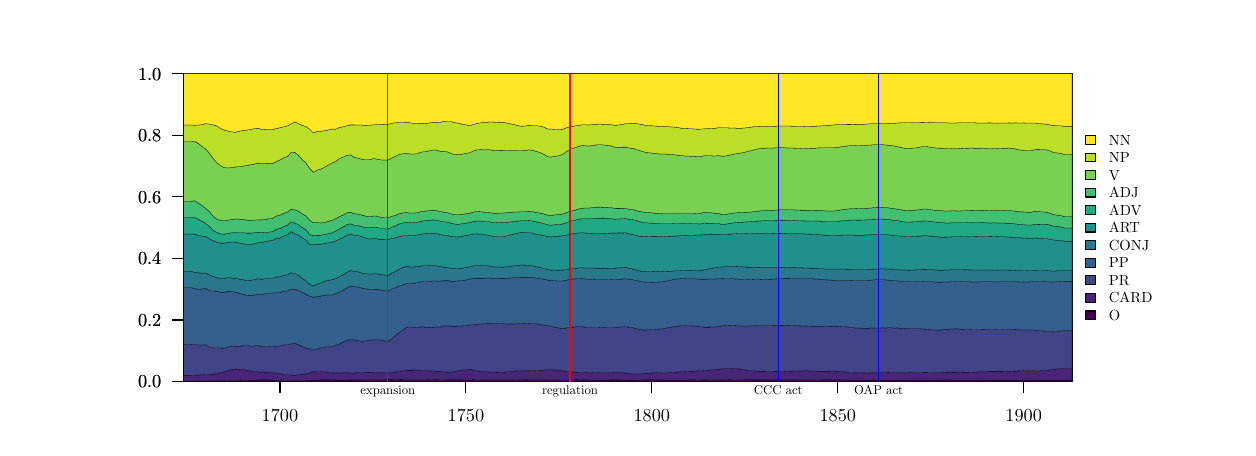
\begin{tikzpicture}[x=1pt,y=1pt]
\definecolor{fillColor}{RGB}{255,255,255}
\path[use as bounding box,fill=fillColor,fill opacity=0.00] (0,0) rectangle (433.62,144.54);
\begin{scope}
\path[clip] (  0.00,  0.00) rectangle (433.62,144.54);
\definecolor{drawColor}{RGB}{0,0,0}

\path[draw=drawColor,line width= 0.4pt,line join=round,line cap=round] ( 91.17, 16.63) -- (359.92, 16.63);

\path[draw=drawColor,line width= 0.4pt,line join=round,line cap=round] ( 91.17, 16.63) -- ( 91.17, 12.67);

\path[draw=drawColor,line width= 0.4pt,line join=round,line cap=round] (158.36, 16.63) -- (158.36, 12.67);

\path[draw=drawColor,line width= 0.4pt,line join=round,line cap=round] (225.54, 16.63) -- (225.54, 12.67);

\path[draw=drawColor,line width= 0.4pt,line join=round,line cap=round] (292.73, 16.63) -- (292.73, 12.67);

\path[draw=drawColor,line width= 0.4pt,line join=round,line cap=round] (359.92, 16.63) -- (359.92, 12.67);

\node[text=drawColor,anchor=base,inner sep=0pt, outer sep=0pt, scale=  0.66] at ( 91.17,  2.38) {1700};

\node[text=drawColor,anchor=base,inner sep=0pt, outer sep=0pt, scale=  0.66] at (158.36,  2.38) {1750};

\node[text=drawColor,anchor=base,inner sep=0pt, outer sep=0pt, scale=  0.66] at (225.54,  2.38) {1800};

\node[text=drawColor,anchor=base,inner sep=0pt, outer sep=0pt, scale=  0.66] at (292.73,  2.38) {1850};

\node[text=drawColor,anchor=base,inner sep=0pt, outer sep=0pt, scale=  0.66] at (359.92,  2.38) {1900};

\path[draw=drawColor,line width= 0.4pt,line join=round,line cap=round] ( 56.23, 16.63) -- ( 56.23,127.91);

\path[draw=drawColor,line width= 0.4pt,line join=round,line cap=round] ( 56.23, 16.63) -- ( 52.27, 16.63);

\path[draw=drawColor,line width= 0.4pt,line join=round,line cap=round] ( 56.23, 38.89) -- ( 52.27, 38.89);

\path[draw=drawColor,line width= 0.4pt,line join=round,line cap=round] ( 56.23, 61.14) -- ( 52.27, 61.14);

\path[draw=drawColor,line width= 0.4pt,line join=round,line cap=round] ( 56.23, 83.40) -- ( 52.27, 83.40);

\path[draw=drawColor,line width= 0.4pt,line join=round,line cap=round] ( 56.23,105.65) -- ( 52.27,105.65);

\path[draw=drawColor,line width= 0.4pt,line join=round,line cap=round] ( 56.23,127.91) -- ( 52.27,127.91);

\node[text=drawColor,anchor=base east,inner sep=0pt, outer sep=0pt, scale=  0.66] at ( 48.31, 14.36) {0.0};

\node[text=drawColor,anchor=base east,inner sep=0pt, outer sep=0pt, scale=  0.66] at ( 48.31, 36.61) {0.2};

\node[text=drawColor,anchor=base east,inner sep=0pt, outer sep=0pt, scale=  0.66] at ( 48.31, 58.87) {0.4};

\node[text=drawColor,anchor=base east,inner sep=0pt, outer sep=0pt, scale=  0.66] at ( 48.31, 81.12) {0.6};

\node[text=drawColor,anchor=base east,inner sep=0pt, outer sep=0pt, scale=  0.66] at ( 48.31,103.38) {0.8};

\node[text=drawColor,anchor=base east,inner sep=0pt, outer sep=0pt, scale=  0.66] at ( 48.31,125.63) {1.0};

\path[draw=drawColor,line width= 0.4pt,line join=round,line cap=round] ( 56.23, 16.63) --
	(377.39, 16.63) --
	(377.39,127.91) --
	( 56.23,127.91) --
	( 56.23, 16.63);
\definecolor{fillColor}{RGB}{68,1,84}

\path[draw=drawColor,line width= 0.1pt,line join=round,line cap=round,fill=fillColor] ( 56.23, 16.63) --
	( 57.58, 16.63) --
	( 58.92, 16.63) --
	( 60.26, 16.63) --
	( 61.61, 16.63) --
	( 62.95, 16.63) --
	( 64.29, 16.63) --
	( 65.64, 16.63) --
	( 66.98, 16.63) --
	( 68.33, 16.63) --
	( 69.67, 16.63) --
	( 71.01, 16.63) --
	( 72.36, 16.63) --
	( 73.70, 16.63) --
	( 75.04, 16.63) --
	( 76.39, 16.63) --
	( 77.73, 16.63) --
	( 79.08, 16.63) --
	( 80.42, 16.63) --
	( 81.76, 16.63) --
	( 83.11, 16.63) --
	( 84.45, 16.63) --
	( 85.79, 16.63) --
	( 87.14, 16.63) --
	( 88.48, 16.63) --
	( 89.83, 16.63) --
	( 91.17, 16.63) --
	( 92.51, 16.63) --
	( 93.86, 16.63) --
	( 95.20, 16.63) --
	( 96.54, 16.63) --
	( 97.89, 16.63) --
	( 99.23, 16.63) --
	(100.58, 16.63) --
	(101.92, 16.63) --
	(103.26, 16.63) --
	(104.61, 16.63) --
	(105.95, 16.63) --
	(107.29, 16.63) --
	(108.64, 16.63) --
	(109.98, 16.63) --
	(111.33, 16.63) --
	(112.67, 16.63) --
	(114.01, 16.63) --
	(115.36, 16.63) --
	(116.70, 16.63) --
	(118.04, 16.63) --
	(119.39, 16.63) --
	(120.73, 16.63) --
	(122.08, 16.63) --
	(123.42, 16.63) --
	(124.76, 16.63) --
	(126.11, 16.63) --
	(127.45, 16.63) --
	(128.79, 16.63) --
	(130.14, 16.63) --
	(131.48, 16.63) --
	(132.83, 16.63) --
	(134.17, 16.63) --
	(135.51, 16.63) --
	(136.86, 16.63) --
	(138.20, 16.63) --
	(139.54, 16.63) --
	(140.89, 16.63) --
	(142.23, 16.63) --
	(143.58, 16.63) --
	(144.92, 16.63) --
	(146.26, 16.63) --
	(147.61, 16.63) --
	(148.95, 16.63) --
	(150.29, 16.63) --
	(151.64, 16.63) --
	(152.98, 16.63) --
	(154.33, 16.63) --
	(155.67, 16.63) --
	(157.01, 16.63) --
	(158.36, 16.63) --
	(159.70, 16.63) --
	(161.04, 16.63) --
	(162.39, 16.63) --
	(163.73, 16.63) --
	(165.08, 16.63) --
	(166.42, 16.63) --
	(167.76, 16.63) --
	(169.11, 16.63) --
	(170.45, 16.63) --
	(171.79, 16.63) --
	(173.14, 16.63) --
	(174.48, 16.63) --
	(175.83, 16.63) --
	(177.17, 16.63) --
	(178.51, 16.63) --
	(179.86, 16.63) --
	(181.20, 16.63) --
	(182.54, 16.63) --
	(183.89, 16.63) --
	(185.23, 16.63) --
	(186.58, 16.63) --
	(187.92, 16.63) --
	(189.26, 16.63) --
	(190.61, 16.63) --
	(191.95, 16.63) --
	(193.29, 16.63) --
	(194.64, 16.63) --
	(195.98, 16.63) --
	(197.33, 16.63) --
	(198.67, 16.63) --
	(200.01, 16.63) --
	(201.36, 16.63) --
	(202.70, 16.63) --
	(204.04, 16.63) --
	(205.39, 16.63) --
	(206.73, 16.63) --
	(208.08, 16.63) --
	(209.42, 16.63) --
	(210.76, 16.63) --
	(212.11, 16.63) --
	(213.45, 16.63) --
	(214.79, 16.63) --
	(216.14, 16.63) --
	(217.48, 16.63) --
	(218.83, 16.63) --
	(220.17, 16.63) --
	(221.51, 16.63) --
	(222.86, 16.63) --
	(224.20, 16.63) --
	(225.54, 16.63) --
	(226.89, 16.63) --
	(228.23, 16.63) --
	(229.58, 16.63) --
	(230.92, 16.63) --
	(232.26, 16.63) --
	(233.61, 16.63) --
	(234.95, 16.63) --
	(236.29, 16.63) --
	(237.64, 16.63) --
	(238.98, 16.63) --
	(240.33, 16.63) --
	(241.67, 16.63) --
	(243.01, 16.63) --
	(244.36, 16.63) --
	(245.70, 16.63) --
	(247.04, 16.63) --
	(248.39, 16.63) --
	(249.73, 16.63) --
	(251.08, 16.63) --
	(252.42, 16.63) --
	(253.76, 16.63) --
	(255.11, 16.63) --
	(256.45, 16.63) --
	(257.79, 16.63) --
	(259.14, 16.63) --
	(260.48, 16.63) --
	(261.83, 16.63) --
	(263.17, 16.63) --
	(264.51, 16.63) --
	(265.86, 16.63) --
	(267.20, 16.63) --
	(268.54, 16.63) --
	(269.89, 16.63) --
	(271.23, 16.63) --
	(272.58, 16.63) --
	(273.92, 16.63) --
	(275.26, 16.63) --
	(276.61, 16.63) --
	(277.95, 16.63) --
	(279.29, 16.63) --
	(280.64, 16.63) --
	(281.98, 16.63) --
	(283.33, 16.63) --
	(284.67, 16.63) --
	(286.01, 16.63) --
	(287.36, 16.63) --
	(288.70, 16.63) --
	(290.04, 16.63) --
	(291.39, 16.63) --
	(292.73, 16.63) --
	(294.08, 16.63) --
	(295.42, 16.63) --
	(296.76, 16.63) --
	(298.11, 16.63) --
	(299.45, 16.63) --
	(300.79, 16.63) --
	(302.14, 16.63) --
	(303.48, 16.63) --
	(304.83, 16.63) --
	(306.17, 16.63) --
	(307.51, 16.63) --
	(308.86, 16.63) --
	(310.20, 16.63) --
	(311.54, 16.63) --
	(312.89, 16.63) --
	(314.23, 16.63) --
	(315.58, 16.63) --
	(316.92, 16.63) --
	(318.26, 16.63) --
	(319.61, 16.63) --
	(320.95, 16.63) --
	(322.29, 16.63) --
	(323.64, 16.63) --
	(324.98, 16.63) --
	(326.33, 16.63) --
	(327.67, 16.63) --
	(329.01, 16.63) --
	(330.36, 16.63) --
	(331.70, 16.63) --
	(333.04, 16.63) --
	(334.39, 16.63) --
	(335.73, 16.63) --
	(337.08, 16.63) --
	(338.42, 16.63) --
	(339.76, 16.63) --
	(341.11, 16.63) --
	(342.45, 16.63) --
	(343.79, 16.63) --
	(345.14, 16.63) --
	(346.48, 16.63) --
	(347.83, 16.63) --
	(349.17, 16.63) --
	(350.51, 16.63) --
	(351.86, 16.63) --
	(353.20, 16.63) --
	(354.54, 16.63) --
	(355.89, 16.63) --
	(357.23, 16.63) --
	(358.58, 16.63) --
	(359.92, 16.63) --
	(361.26, 16.63) --
	(362.61, 16.63) --
	(363.95, 16.63) --
	(365.29, 16.63) --
	(366.64, 16.63) --
	(367.98, 16.63) --
	(369.33, 16.63) --
	(370.67, 16.63) --
	(372.01, 16.63) --
	(373.36, 16.63) --
	(374.70, 16.63) --
	(376.04, 16.63) --
	(377.39, 16.63) --
	(377.39, 17.16) --
	(376.04, 17.16) --
	(374.70, 17.16) --
	(373.36, 17.16) --
	(372.01, 17.16) --
	(370.67, 17.16) --
	(369.33, 17.17) --
	(367.98, 17.17) --
	(366.64, 17.17) --
	(365.29, 17.19) --
	(363.95, 17.21) --
	(362.61, 17.21) --
	(361.26, 17.21) --
	(359.92, 17.21) --
	(358.58, 17.20) --
	(357.23, 17.19) --
	(355.89, 17.17) --
	(354.54, 17.16) --
	(353.20, 17.17) --
	(351.86, 17.17) --
	(350.51, 17.17) --
	(349.17, 17.17) --
	(347.83, 17.19) --
	(346.48, 17.19) --
	(345.14, 17.20) --
	(343.79, 17.21) --
	(342.45, 17.23) --
	(341.11, 17.23) --
	(339.76, 17.24) --
	(338.42, 17.24) --
	(337.08, 17.26) --
	(335.73, 17.26) --
	(334.39, 17.26) --
	(333.04, 17.28) --
	(331.70, 17.28) --
	(330.36, 17.26) --
	(329.01, 17.24) --
	(327.67, 17.23) --
	(326.33, 17.22) --
	(324.98, 17.20) --
	(323.64, 17.21) --
	(322.29, 17.21) --
	(320.95, 17.22) --
	(319.61, 17.23) --
	(318.26, 17.23) --
	(316.92, 17.24) --
	(315.58, 17.24) --
	(314.23, 17.23) --
	(312.89, 17.23) --
	(311.54, 17.24) --
	(310.20, 17.24) --
	(308.86, 17.23) --
	(307.51, 17.22) --
	(306.17, 17.21) --
	(304.83, 17.21) --
	(303.48, 17.20) --
	(302.14, 17.22) --
	(300.79, 17.22) --
	(299.45, 17.22) --
	(298.11, 17.21) --
	(296.76, 17.23) --
	(295.42, 17.25) --
	(294.08, 17.26) --
	(292.73, 17.29) --
	(291.39, 17.30) --
	(290.04, 17.30) --
	(288.70, 17.30) --
	(287.36, 17.31) --
	(286.01, 17.32) --
	(284.67, 17.34) --
	(283.33, 17.35) --
	(281.98, 17.35) --
	(280.64, 17.34) --
	(279.29, 17.33) --
	(277.95, 17.31) --
	(276.61, 17.31) --
	(275.26, 17.32) --
	(273.92, 17.31) --
	(272.58, 17.30) --
	(271.23, 17.30) --
	(269.89, 17.29) --
	(268.54, 17.26) --
	(267.20, 17.27) --
	(265.86, 17.27) --
	(264.51, 17.27) --
	(263.17, 17.27) --
	(261.83, 17.29) --
	(260.48, 17.30) --
	(259.14, 17.31) --
	(257.79, 17.33) --
	(256.45, 17.34) --
	(255.11, 17.35) --
	(253.76, 17.36) --
	(252.42, 17.38) --
	(251.08, 17.37) --
	(249.73, 17.34) --
	(248.39, 17.33) --
	(247.04, 17.33) --
	(245.70, 17.32) --
	(244.36, 17.31) --
	(243.01, 17.32) --
	(241.67, 17.32) --
	(240.33, 17.30) --
	(238.98, 17.27) --
	(237.64, 17.26) --
	(236.29, 17.25) --
	(234.95, 17.24) --
	(233.61, 17.23) --
	(232.26, 17.24) --
	(230.92, 17.25) --
	(229.58, 17.26) --
	(228.23, 17.28) --
	(226.89, 17.29) --
	(225.54, 17.29) --
	(224.20, 17.28) --
	(222.86, 17.26) --
	(221.51, 17.22) --
	(220.17, 17.20) --
	(218.83, 17.17) --
	(217.48, 17.18) --
	(216.14, 17.21) --
	(214.79, 17.23) --
	(213.45, 17.27) --
	(212.11, 17.28) --
	(210.76, 17.27) --
	(209.42, 17.25) --
	(208.08, 17.25) --
	(206.73, 17.23) --
	(205.39, 17.23) --
	(204.04, 17.25) --
	(202.70, 17.26) --
	(201.36, 17.30) --
	(200.01, 17.32) --
	(198.67, 17.36) --
	(197.33, 17.37) --
	(195.98, 17.40) --
	(194.64, 17.39) --
	(193.29, 17.40) --
	(191.95, 17.41) --
	(190.61, 17.42) --
	(189.26, 17.40) --
	(187.92, 17.41) --
	(186.58, 17.41) --
	(185.23, 17.41) --
	(183.89, 17.42) --
	(182.54, 17.44) --
	(181.20, 17.44) --
	(179.86, 17.45) --
	(178.51, 17.44) --
	(177.17, 17.41) --
	(175.83, 17.38) --
	(174.48, 17.35) --
	(173.14, 17.35) --
	(171.79, 17.33) --
	(170.45, 17.32) --
	(169.11, 17.32) --
	(167.76, 17.32) --
	(166.42, 17.32) --
	(165.08, 17.33) --
	(163.73, 17.34) --
	(162.39, 17.35) --
	(161.04, 17.36) --
	(159.70, 17.35) --
	(158.36, 17.34) --
	(157.01, 17.31) --
	(155.67, 17.30) --
	(154.33, 17.28) --
	(152.98, 17.29) --
	(151.64, 17.30) --
	(150.29, 17.32) --
	(148.95, 17.34) --
	(147.61, 17.37) --
	(146.26, 17.35) --
	(144.92, 17.36) --
	(143.58, 17.38) --
	(142.23, 17.40) --
	(140.89, 17.38) --
	(139.54, 17.39) --
	(138.20, 17.40) --
	(136.86, 17.41) --
	(135.51, 17.44) --
	(134.17, 17.46) --
	(132.83, 17.49) --
	(131.48, 17.50) --
	(130.14, 17.52) --
	(128.79, 17.42) --
	(127.45, 17.40) --
	(126.11, 17.38) --
	(124.76, 17.35) --
	(123.42, 17.30) --
	(122.08, 17.34) --
	(120.73, 17.31) --
	(119.39, 17.27) --
	(118.04, 17.26) --
	(116.70, 17.27) --
	(115.36, 17.26) --
	(114.01, 17.26) --
	(112.67, 17.24) --
	(111.33, 17.28) --
	(109.98, 17.26) --
	(108.64, 17.27) --
	(107.29, 17.29) --
	(105.95, 17.30) --
	(104.61, 17.21) --
	(103.26, 17.19) --
	(101.92, 17.14) --
	(100.58, 17.06) --
	( 99.23, 17.02) --
	( 97.89, 17.02) --
	( 96.54, 16.95) --
	( 95.20, 16.89) --
	( 93.86, 16.87) --
	( 92.51, 16.89) --
	( 91.17, 16.96) --
	( 89.83, 17.07) --
	( 88.48, 17.19) --
	( 87.14, 17.27) --
	( 85.79, 17.31) --
	( 84.45, 17.28) --
	( 83.11, 17.26) --
	( 81.76, 17.17) --
	( 80.42, 17.14) --
	( 79.08, 17.13) --
	( 77.73, 17.12) --
	( 76.39, 17.07) --
	( 75.04, 17.06) --
	( 73.70, 17.02) --
	( 72.36, 16.98) --
	( 71.01, 16.91) --
	( 69.67, 16.90) --
	( 68.33, 16.88) --
	( 66.98, 16.87) --
	( 65.64, 16.84) --
	( 64.29, 16.80) --
	( 62.95, 16.80) --
	( 61.61, 16.83) --
	( 60.26, 16.79) --
	( 58.92, 16.78) --
	( 57.58, 16.78) --
	( 56.23, 16.78) --
	cycle;
\definecolor{fillColor}{RGB}{72,37,118}

\path[draw=drawColor,line width= 0.1pt,line join=round,line cap=round,fill=fillColor] ( 56.23, 16.78) --
	( 57.58, 16.78) --
	( 58.92, 16.78) --
	( 60.26, 16.79) --
	( 61.61, 16.83) --
	( 62.95, 16.80) --
	( 64.29, 16.80) --
	( 65.64, 16.84) --
	( 66.98, 16.87) --
	( 68.33, 16.88) --
	( 69.67, 16.90) --
	( 71.01, 16.91) --
	( 72.36, 16.98) --
	( 73.70, 17.02) --
	( 75.04, 17.06) --
	( 76.39, 17.07) --
	( 77.73, 17.12) --
	( 79.08, 17.13) --
	( 80.42, 17.14) --
	( 81.76, 17.17) --
	( 83.11, 17.26) --
	( 84.45, 17.28) --
	( 85.79, 17.31) --
	( 87.14, 17.27) --
	( 88.48, 17.19) --
	( 89.83, 17.07) --
	( 91.17, 16.96) --
	( 92.51, 16.89) --
	( 93.86, 16.87) --
	( 95.20, 16.89) --
	( 96.54, 16.95) --
	( 97.89, 17.02) --
	( 99.23, 17.02) --
	(100.58, 17.06) --
	(101.92, 17.14) --
	(103.26, 17.19) --
	(104.61, 17.21) --
	(105.95, 17.30) --
	(107.29, 17.29) --
	(108.64, 17.27) --
	(109.98, 17.26) --
	(111.33, 17.28) --
	(112.67, 17.24) --
	(114.01, 17.26) --
	(115.36, 17.26) --
	(116.70, 17.27) --
	(118.04, 17.26) --
	(119.39, 17.27) --
	(120.73, 17.31) --
	(122.08, 17.34) --
	(123.42, 17.30) --
	(124.76, 17.35) --
	(126.11, 17.38) --
	(127.45, 17.40) --
	(128.79, 17.42) --
	(130.14, 17.52) --
	(131.48, 17.50) --
	(132.83, 17.49) --
	(134.17, 17.46) --
	(135.51, 17.44) --
	(136.86, 17.41) --
	(138.20, 17.40) --
	(139.54, 17.39) --
	(140.89, 17.38) --
	(142.23, 17.40) --
	(143.58, 17.38) --
	(144.92, 17.36) --
	(146.26, 17.35) --
	(147.61, 17.37) --
	(148.95, 17.34) --
	(150.29, 17.32) --
	(151.64, 17.30) --
	(152.98, 17.29) --
	(154.33, 17.28) --
	(155.67, 17.30) --
	(157.01, 17.31) --
	(158.36, 17.34) --
	(159.70, 17.35) --
	(161.04, 17.36) --
	(162.39, 17.35) --
	(163.73, 17.34) --
	(165.08, 17.33) --
	(166.42, 17.32) --
	(167.76, 17.32) --
	(169.11, 17.32) --
	(170.45, 17.32) --
	(171.79, 17.33) --
	(173.14, 17.35) --
	(174.48, 17.35) --
	(175.83, 17.38) --
	(177.17, 17.41) --
	(178.51, 17.44) --
	(179.86, 17.45) --
	(181.20, 17.44) --
	(182.54, 17.44) --
	(183.89, 17.42) --
	(185.23, 17.41) --
	(186.58, 17.41) --
	(187.92, 17.41) --
	(189.26, 17.40) --
	(190.61, 17.42) --
	(191.95, 17.41) --
	(193.29, 17.40) --
	(194.64, 17.39) --
	(195.98, 17.40) --
	(197.33, 17.37) --
	(198.67, 17.36) --
	(200.01, 17.32) --
	(201.36, 17.30) --
	(202.70, 17.26) --
	(204.04, 17.25) --
	(205.39, 17.23) --
	(206.73, 17.23) --
	(208.08, 17.25) --
	(209.42, 17.25) --
	(210.76, 17.27) --
	(212.11, 17.28) --
	(213.45, 17.27) --
	(214.79, 17.23) --
	(216.14, 17.21) --
	(217.48, 17.18) --
	(218.83, 17.17) --
	(220.17, 17.20) --
	(221.51, 17.22) --
	(222.86, 17.26) --
	(224.20, 17.28) --
	(225.54, 17.29) --
	(226.89, 17.29) --
	(228.23, 17.28) --
	(229.58, 17.26) --
	(230.92, 17.25) --
	(232.26, 17.24) --
	(233.61, 17.23) --
	(234.95, 17.24) --
	(236.29, 17.25) --
	(237.64, 17.26) --
	(238.98, 17.27) --
	(240.33, 17.30) --
	(241.67, 17.32) --
	(243.01, 17.32) --
	(244.36, 17.31) --
	(245.70, 17.32) --
	(247.04, 17.33) --
	(248.39, 17.33) --
	(249.73, 17.34) --
	(251.08, 17.37) --
	(252.42, 17.38) --
	(253.76, 17.36) --
	(255.11, 17.35) --
	(256.45, 17.34) --
	(257.79, 17.33) --
	(259.14, 17.31) --
	(260.48, 17.30) --
	(261.83, 17.29) --
	(263.17, 17.27) --
	(264.51, 17.27) --
	(265.86, 17.27) --
	(267.20, 17.27) --
	(268.54, 17.26) --
	(269.89, 17.29) --
	(271.23, 17.30) --
	(272.58, 17.30) --
	(273.92, 17.31) --
	(275.26, 17.32) --
	(276.61, 17.31) --
	(277.95, 17.31) --
	(279.29, 17.33) --
	(280.64, 17.34) --
	(281.98, 17.35) --
	(283.33, 17.35) --
	(284.67, 17.34) --
	(286.01, 17.32) --
	(287.36, 17.31) --
	(288.70, 17.30) --
	(290.04, 17.30) --
	(291.39, 17.30) --
	(292.73, 17.29) --
	(294.08, 17.26) --
	(295.42, 17.25) --
	(296.76, 17.23) --
	(298.11, 17.21) --
	(299.45, 17.22) --
	(300.79, 17.22) --
	(302.14, 17.22) --
	(303.48, 17.20) --
	(304.83, 17.21) --
	(306.17, 17.21) --
	(307.51, 17.22) --
	(308.86, 17.23) --
	(310.20, 17.24) --
	(311.54, 17.24) --
	(312.89, 17.23) --
	(314.23, 17.23) --
	(315.58, 17.24) --
	(316.92, 17.24) --
	(318.26, 17.23) --
	(319.61, 17.23) --
	(320.95, 17.22) --
	(322.29, 17.21) --
	(323.64, 17.21) --
	(324.98, 17.20) --
	(326.33, 17.22) --
	(327.67, 17.23) --
	(329.01, 17.24) --
	(330.36, 17.26) --
	(331.70, 17.28) --
	(333.04, 17.28) --
	(334.39, 17.26) --
	(335.73, 17.26) --
	(337.08, 17.26) --
	(338.42, 17.24) --
	(339.76, 17.24) --
	(341.11, 17.23) --
	(342.45, 17.23) --
	(343.79, 17.21) --
	(345.14, 17.20) --
	(346.48, 17.19) --
	(347.83, 17.19) --
	(349.17, 17.17) --
	(350.51, 17.17) --
	(351.86, 17.17) --
	(353.20, 17.17) --
	(354.54, 17.16) --
	(355.89, 17.17) --
	(357.23, 17.19) --
	(358.58, 17.20) --
	(359.92, 17.21) --
	(361.26, 17.21) --
	(362.61, 17.21) --
	(363.95, 17.21) --
	(365.29, 17.19) --
	(366.64, 17.17) --
	(367.98, 17.17) --
	(369.33, 17.17) --
	(370.67, 17.16) --
	(372.01, 17.16) --
	(373.36, 17.16) --
	(374.70, 17.16) --
	(376.04, 17.16) --
	(377.39, 17.16) --
	(377.39, 21.46) --
	(376.04, 21.46) --
	(374.70, 21.46) --
	(373.36, 21.31) --
	(372.01, 21.26) --
	(370.67, 21.09) --
	(369.33, 20.83) --
	(367.98, 20.68) --
	(366.64, 20.62) --
	(365.29, 20.57) --
	(363.95, 20.57) --
	(362.61, 20.66) --
	(361.26, 20.68) --
	(359.92, 20.62) --
	(358.58, 20.55) --
	(357.23, 20.45) --
	(355.89, 20.38) --
	(354.54, 20.33) --
	(353.20, 20.38) --
	(351.86, 20.41) --
	(350.51, 20.44) --
	(349.17, 20.41) --
	(347.83, 20.44) --
	(346.48, 20.35) --
	(345.14, 20.26) --
	(343.79, 20.17) --
	(342.45, 20.11) --
	(341.11, 20.02) --
	(339.76, 20.03) --
	(338.42, 20.06) --
	(337.08, 20.09) --
	(335.73, 20.07) --
	(334.39, 20.07) --
	(333.04, 20.09) --
	(331.70, 20.03) --
	(330.36, 19.97) --
	(329.01, 19.97) --
	(327.67, 19.95) --
	(326.33, 19.92) --
	(324.98, 19.89) --
	(323.64, 19.89) --
	(322.29, 19.92) --
	(320.95, 19.96) --
	(319.61, 19.95) --
	(318.26, 20.00) --
	(316.92, 20.01) --
	(315.58, 20.01) --
	(314.23, 20.00) --
	(312.89, 20.01) --
	(311.54, 19.99) --
	(310.20, 19.97) --
	(308.86, 19.90) --
	(307.51, 19.83) --
	(306.17, 19.82) --
	(304.83, 19.81) --
	(303.48, 19.79) --
	(302.14, 19.80) --
	(300.79, 19.82) --
	(299.45, 19.80) --
	(298.11, 19.80) --
	(296.76, 19.95) --
	(295.42, 20.10) --
	(294.08, 20.25) --
	(292.73, 20.39) --
	(291.39, 20.46) --
	(290.04, 20.44) --
	(288.70, 20.42) --
	(287.36, 20.40) --
	(286.01, 20.41) --
	(284.67, 20.45) --
	(283.33, 20.51) --
	(281.98, 20.52) --
	(280.64, 20.54) --
	(279.29, 20.50) --
	(277.95, 20.49) --
	(276.61, 20.45) --
	(275.26, 20.40) --
	(273.92, 20.35) --
	(272.58, 20.32) --
	(271.23, 20.34) --
	(269.89, 20.34) --
	(268.54, 20.36) --
	(267.20, 20.38) --
	(265.86, 20.40) --
	(264.51, 20.41) --
	(263.17, 20.47) --
	(261.83, 20.59) --
	(260.48, 20.72) --
	(259.14, 20.91) --
	(257.79, 21.11) --
	(256.45, 21.27) --
	(255.11, 21.37) --
	(253.76, 21.47) --
	(252.42, 21.43) --
	(251.08, 21.28) --
	(249.73, 21.15) --
	(248.39, 21.05) --
	(247.04, 20.86) --
	(245.70, 20.74) --
	(244.36, 20.62) --
	(243.01, 20.57) --
	(241.67, 20.50) --
	(240.33, 20.43) --
	(238.98, 20.40) --
	(237.64, 20.34) --
	(236.29, 20.24) --
	(234.95, 20.11) --
	(233.61, 20.03) --
	(232.26, 19.96) --
	(230.92, 19.95) --
	(229.58, 19.92) --
	(228.23, 19.95) --
	(226.89, 19.87) --
	(225.54, 19.80) --
	(224.20, 19.73) --
	(222.86, 19.56) --
	(221.51, 19.42) --
	(220.17, 19.38) --
	(218.83, 19.38) --
	(217.48, 19.55) --
	(216.14, 19.75) --
	(214.79, 19.87) --
	(213.45, 19.98) --
	(212.11, 20.03) --
	(210.76, 19.92) --
	(209.42, 19.85) --
	(208.08, 19.88) --
	(206.73, 19.87) --
	(205.39, 19.91) --
	(204.04, 19.99) --
	(202.70, 20.02) --
	(201.36, 19.96) --
	(200.01, 19.95) --
	(198.67, 20.05) --
	(197.33, 20.10) --
	(195.98, 20.21) --
	(194.64, 20.34) --
	(193.29, 20.63) --
	(191.95, 20.76) --
	(190.61, 20.87) --
	(189.26, 20.92) --
	(187.92, 21.04) --
	(186.58, 20.84) --
	(185.23, 20.73) --
	(183.89, 20.63) --
	(182.54, 20.60) --
	(181.20, 20.51) --
	(179.86, 20.61) --
	(178.51, 20.68) --
	(177.17, 20.61) --
	(175.83, 20.43) --
	(174.48, 20.32) --
	(173.14, 20.17) --
	(171.79, 20.03) --
	(170.45, 19.99) --
	(169.11, 20.09) --
	(167.76, 20.08) --
	(166.42, 20.16) --
	(165.08, 20.29) --
	(163.73, 20.37) --
	(162.39, 20.51) --
	(161.04, 20.78) --
	(159.70, 21.12) --
	(158.36, 20.97) --
	(157.01, 20.85) --
	(155.67, 20.55) --
	(154.33, 20.35) --
	(152.98, 20.05) --
	(151.64, 20.07) --
	(150.29, 20.10) --
	(148.95, 20.39) --
	(147.61, 20.42) --
	(146.26, 20.48) --
	(144.92, 20.57) --
	(143.58, 20.67) --
	(142.23, 20.69) --
	(140.89, 20.84) --
	(139.54, 20.80) --
	(138.20, 20.79) --
	(136.86, 20.78) --
	(135.51, 20.54) --
	(134.17, 20.24) --
	(132.83, 20.11) --
	(131.48, 19.91) --
	(130.14, 19.79) --
	(128.79, 19.88) --
	(127.45, 20.03) --
	(126.11, 19.96) --
	(124.76, 19.98) --
	(123.42, 20.07) --
	(122.08, 20.02) --
	(120.73, 19.84) --
	(119.39, 19.83) --
	(118.04, 19.79) --
	(116.70, 19.76) --
	(115.36, 19.82) --
	(114.01, 19.83) --
	(112.67, 19.75) --
	(111.33, 19.86) --
	(109.98, 19.78) --
	(108.64, 19.99) --
	(107.29, 20.20) --
	(105.95, 20.25) --
	(104.61, 20.19) --
	(103.26, 20.32) --
	(101.92, 19.77) --
	(100.58, 19.44) --
	( 99.23, 19.36) --
	( 97.89, 19.24) --
	( 96.54, 18.93) --
	( 95.20, 19.10) --
	( 93.86, 19.15) --
	( 92.51, 19.26) --
	( 91.17, 19.51) --
	( 89.83, 19.73) --
	( 88.48, 19.83) --
	( 87.14, 19.97) --
	( 85.79, 20.08) --
	( 84.45, 20.09) --
	( 83.11, 20.14) --
	( 81.76, 20.31) --
	( 80.42, 20.50) --
	( 79.08, 20.83) --
	( 77.73, 21.03) --
	( 76.39, 21.07) --
	( 75.04, 21.21) --
	( 73.70, 21.02) --
	( 72.36, 20.61) --
	( 71.01, 20.15) --
	( 69.67, 19.90) --
	( 68.33, 19.52) --
	( 66.98, 19.34) --
	( 65.64, 19.17) --
	( 64.29, 19.19) --
	( 62.95, 19.14) --
	( 61.61, 19.04) --
	( 60.26, 18.90) --
	( 58.92, 18.95) --
	( 57.58, 18.95) --
	( 56.23, 18.95) --
	cycle;
\definecolor{fillColor}{RGB}{65,68,135}

\path[draw=drawColor,line width= 0.1pt,line join=round,line cap=round,fill=fillColor] ( 56.23, 18.95) --
	( 57.58, 18.95) --
	( 58.92, 18.95) --
	( 60.26, 18.90) --
	( 61.61, 19.04) --
	( 62.95, 19.14) --
	( 64.29, 19.19) --
	( 65.64, 19.17) --
	( 66.98, 19.34) --
	( 68.33, 19.52) --
	( 69.67, 19.90) --
	( 71.01, 20.15) --
	( 72.36, 20.61) --
	( 73.70, 21.02) --
	( 75.04, 21.21) --
	( 76.39, 21.07) --
	( 77.73, 21.03) --
	( 79.08, 20.83) --
	( 80.42, 20.50) --
	( 81.76, 20.31) --
	( 83.11, 20.14) --
	( 84.45, 20.09) --
	( 85.79, 20.08) --
	( 87.14, 19.97) --
	( 88.48, 19.83) --
	( 89.83, 19.73) --
	( 91.17, 19.51) --
	( 92.51, 19.26) --
	( 93.86, 19.15) --
	( 95.20, 19.10) --
	( 96.54, 18.93) --
	( 97.89, 19.24) --
	( 99.23, 19.36) --
	(100.58, 19.44) --
	(101.92, 19.77) --
	(103.26, 20.32) --
	(104.61, 20.19) --
	(105.95, 20.25) --
	(107.29, 20.20) --
	(108.64, 19.99) --
	(109.98, 19.78) --
	(111.33, 19.86) --
	(112.67, 19.75) --
	(114.01, 19.83) --
	(115.36, 19.82) --
	(116.70, 19.76) --
	(118.04, 19.79) --
	(119.39, 19.83) --
	(120.73, 19.84) --
	(122.08, 20.02) --
	(123.42, 20.07) --
	(124.76, 19.98) --
	(126.11, 19.96) --
	(127.45, 20.03) --
	(128.79, 19.88) --
	(130.14, 19.79) --
	(131.48, 19.91) --
	(132.83, 20.11) --
	(134.17, 20.24) --
	(135.51, 20.54) --
	(136.86, 20.78) --
	(138.20, 20.79) --
	(139.54, 20.80) --
	(140.89, 20.84) --
	(142.23, 20.69) --
	(143.58, 20.67) --
	(144.92, 20.57) --
	(146.26, 20.48) --
	(147.61, 20.42) --
	(148.95, 20.39) --
	(150.29, 20.10) --
	(151.64, 20.07) --
	(152.98, 20.05) --
	(154.33, 20.35) --
	(155.67, 20.55) --
	(157.01, 20.85) --
	(158.36, 20.97) --
	(159.70, 21.12) --
	(161.04, 20.78) --
	(162.39, 20.51) --
	(163.73, 20.37) --
	(165.08, 20.29) --
	(166.42, 20.16) --
	(167.76, 20.08) --
	(169.11, 20.09) --
	(170.45, 19.99) --
	(171.79, 20.03) --
	(173.14, 20.17) --
	(174.48, 20.32) --
	(175.83, 20.43) --
	(177.17, 20.61) --
	(178.51, 20.68) --
	(179.86, 20.61) --
	(181.20, 20.51) --
	(182.54, 20.60) --
	(183.89, 20.63) --
	(185.23, 20.73) --
	(186.58, 20.84) --
	(187.92, 21.04) --
	(189.26, 20.92) --
	(190.61, 20.87) --
	(191.95, 20.76) --
	(193.29, 20.63) --
	(194.64, 20.34) --
	(195.98, 20.21) --
	(197.33, 20.10) --
	(198.67, 20.05) --
	(200.01, 19.95) --
	(201.36, 19.96) --
	(202.70, 20.02) --
	(204.04, 19.99) --
	(205.39, 19.91) --
	(206.73, 19.87) --
	(208.08, 19.88) --
	(209.42, 19.85) --
	(210.76, 19.92) --
	(212.11, 20.03) --
	(213.45, 19.98) --
	(214.79, 19.87) --
	(216.14, 19.75) --
	(217.48, 19.55) --
	(218.83, 19.38) --
	(220.17, 19.38) --
	(221.51, 19.42) --
	(222.86, 19.56) --
	(224.20, 19.73) --
	(225.54, 19.80) --
	(226.89, 19.87) --
	(228.23, 19.95) --
	(229.58, 19.92) --
	(230.92, 19.95) --
	(232.26, 19.96) --
	(233.61, 20.03) --
	(234.95, 20.11) --
	(236.29, 20.24) --
	(237.64, 20.34) --
	(238.98, 20.40) --
	(240.33, 20.43) --
	(241.67, 20.50) --
	(243.01, 20.57) --
	(244.36, 20.62) --
	(245.70, 20.74) --
	(247.04, 20.86) --
	(248.39, 21.05) --
	(249.73, 21.15) --
	(251.08, 21.28) --
	(252.42, 21.43) --
	(253.76, 21.47) --
	(255.11, 21.37) --
	(256.45, 21.27) --
	(257.79, 21.11) --
	(259.14, 20.91) --
	(260.48, 20.72) --
	(261.83, 20.59) --
	(263.17, 20.47) --
	(264.51, 20.41) --
	(265.86, 20.40) --
	(267.20, 20.38) --
	(268.54, 20.36) --
	(269.89, 20.34) --
	(271.23, 20.34) --
	(272.58, 20.32) --
	(273.92, 20.35) --
	(275.26, 20.40) --
	(276.61, 20.45) --
	(277.95, 20.49) --
	(279.29, 20.50) --
	(280.64, 20.54) --
	(281.98, 20.52) --
	(283.33, 20.51) --
	(284.67, 20.45) --
	(286.01, 20.41) --
	(287.36, 20.40) --
	(288.70, 20.42) --
	(290.04, 20.44) --
	(291.39, 20.46) --
	(292.73, 20.39) --
	(294.08, 20.25) --
	(295.42, 20.10) --
	(296.76, 19.95) --
	(298.11, 19.80) --
	(299.45, 19.80) --
	(300.79, 19.82) --
	(302.14, 19.80) --
	(303.48, 19.79) --
	(304.83, 19.81) --
	(306.17, 19.82) --
	(307.51, 19.83) --
	(308.86, 19.90) --
	(310.20, 19.97) --
	(311.54, 19.99) --
	(312.89, 20.01) --
	(314.23, 20.00) --
	(315.58, 20.01) --
	(316.92, 20.01) --
	(318.26, 20.00) --
	(319.61, 19.95) --
	(320.95, 19.96) --
	(322.29, 19.92) --
	(323.64, 19.89) --
	(324.98, 19.89) --
	(326.33, 19.92) --
	(327.67, 19.95) --
	(329.01, 19.97) --
	(330.36, 19.97) --
	(331.70, 20.03) --
	(333.04, 20.09) --
	(334.39, 20.07) --
	(335.73, 20.07) --
	(337.08, 20.09) --
	(338.42, 20.06) --
	(339.76, 20.03) --
	(341.11, 20.02) --
	(342.45, 20.11) --
	(343.79, 20.17) --
	(345.14, 20.26) --
	(346.48, 20.35) --
	(347.83, 20.44) --
	(349.17, 20.41) --
	(350.51, 20.44) --
	(351.86, 20.41) --
	(353.20, 20.38) --
	(354.54, 20.33) --
	(355.89, 20.38) --
	(357.23, 20.45) --
	(358.58, 20.55) --
	(359.92, 20.62) --
	(361.26, 20.68) --
	(362.61, 20.66) --
	(363.95, 20.57) --
	(365.29, 20.57) --
	(366.64, 20.62) --
	(367.98, 20.68) --
	(369.33, 20.83) --
	(370.67, 21.09) --
	(372.01, 21.26) --
	(373.36, 21.31) --
	(374.70, 21.46) --
	(376.04, 21.46) --
	(377.39, 21.46) --
	(377.39, 35.19) --
	(376.04, 35.19) --
	(374.70, 35.19) --
	(373.36, 35.00) --
	(372.01, 34.80) --
	(370.67, 34.61) --
	(369.33, 34.64) --
	(367.98, 34.79) --
	(366.64, 34.98) --
	(365.29, 35.07) --
	(363.95, 35.27) --
	(362.61, 35.32) --
	(361.26, 35.29) --
	(359.92, 35.29) --
	(358.58, 35.38) --
	(357.23, 35.44) --
	(355.89, 35.41) --
	(354.54, 35.50) --
	(353.20, 35.46) --
	(351.86, 35.42) --
	(350.51, 35.39) --
	(349.17, 35.45) --
	(347.83, 35.48) --
	(346.48, 35.49) --
	(345.14, 35.53) --
	(343.79, 35.48) --
	(342.45, 35.41) --
	(341.11, 35.42) --
	(339.76, 35.45) --
	(338.42, 35.49) --
	(337.08, 35.65) --
	(335.73, 35.72) --
	(334.39, 35.68) --
	(333.04, 35.62) --
	(331.70, 35.50) --
	(330.36, 35.34) --
	(329.01, 35.24) --
	(327.67, 35.30) --
	(326.33, 35.46) --
	(324.98, 35.55) --
	(323.64, 35.64) --
	(322.29, 35.72) --
	(320.95, 35.72) --
	(319.61, 35.73) --
	(318.26, 35.79) --
	(316.92, 35.89) --
	(315.58, 35.94) --
	(314.23, 36.07) --
	(312.89, 36.03) --
	(311.54, 36.11) --
	(310.20, 36.04) --
	(308.86, 36.08) --
	(307.51, 35.98) --
	(306.17, 36.05) --
	(304.83, 36.01) --
	(303.48, 35.94) --
	(302.14, 35.92) --
	(300.79, 36.01) --
	(299.45, 36.00) --
	(298.11, 36.12) --
	(296.76, 36.37) --
	(295.42, 36.53) --
	(294.08, 36.58) --
	(292.73, 36.67) --
	(291.39, 36.71) --
	(290.04, 36.68) --
	(288.70, 36.62) --
	(287.36, 36.65) --
	(286.01, 36.65) --
	(284.67, 36.67) --
	(283.33, 36.69) --
	(281.98, 36.75) --
	(280.64, 36.77) --
	(279.29, 36.78) --
	(277.95, 36.81) --
	(276.61, 36.91) --
	(275.26, 36.95) --
	(273.92, 37.00) --
	(272.58, 37.04) --
	(271.23, 37.02) --
	(269.89, 36.97) --
	(268.54, 36.95) --
	(267.20, 36.92) --
	(265.86, 36.92) --
	(264.51, 36.92) --
	(263.17, 36.88) --
	(261.83, 36.81) --
	(260.48, 36.74) --
	(259.14, 36.73) --
	(257.79, 36.78) --
	(256.45, 36.86) --
	(255.11, 36.88) --
	(253.76, 36.97) --
	(252.42, 36.93) --
	(251.08, 36.82) --
	(249.73, 36.59) --
	(248.39, 36.36) --
	(247.04, 36.34) --
	(245.70, 36.33) --
	(244.36, 36.32) --
	(243.01, 36.49) --
	(241.67, 36.74) --
	(240.33, 36.73) --
	(238.98, 36.85) --
	(237.64, 36.87) --
	(236.29, 36.85) --
	(234.95, 36.71) --
	(233.61, 36.62) --
	(232.26, 36.25) --
	(230.92, 36.03) --
	(229.58, 35.77) --
	(228.23, 35.63) --
	(226.89, 35.43) --
	(225.54, 35.37) --
	(224.20, 35.37) --
	(222.86, 35.24) --
	(221.51, 35.44) --
	(220.17, 35.69) --
	(218.83, 36.10) --
	(217.48, 36.25) --
	(216.14, 36.56) --
	(214.79, 36.45) --
	(213.45, 36.36) --
	(212.11, 36.17) --
	(210.76, 36.16) --
	(209.42, 36.20) --
	(208.08, 36.24) --
	(206.73, 36.15) --
	(205.39, 36.17) --
	(204.04, 36.18) --
	(202.70, 36.09) --
	(201.36, 36.31) --
	(200.01, 36.55) --
	(198.67, 36.51) --
	(197.33, 36.34) --
	(195.98, 36.31) --
	(194.64, 36.00) --
	(193.29, 35.89) --
	(191.95, 36.02) --
	(190.61, 36.28) --
	(189.26, 36.58) --
	(187.92, 36.90) --
	(186.58, 37.11) --
	(185.23, 37.32) --
	(183.89, 37.53) --
	(182.54, 37.65) --
	(181.20, 37.69) --
	(179.86, 37.73) --
	(178.51, 37.66) --
	(177.17, 37.56) --
	(175.83, 37.47) --
	(174.48, 37.53) --
	(173.14, 37.45) --
	(171.79, 37.60) --
	(170.45, 37.65) --
	(169.11, 37.65) --
	(167.76, 37.71) --
	(166.42, 37.80) --
	(165.08, 37.56) --
	(163.73, 37.46) --
	(162.39, 37.43) --
	(161.04, 37.27) --
	(159.70, 37.12) --
	(158.36, 36.89) --
	(157.01, 36.76) --
	(155.67, 36.72) --
	(154.33, 36.68) --
	(152.98, 36.69) --
	(151.64, 36.86) --
	(150.29, 36.70) --
	(148.95, 36.36) --
	(147.61, 36.42) --
	(146.26, 36.31) --
	(144.92, 36.22) --
	(143.58, 36.32) --
	(142.23, 36.49) --
	(140.89, 36.19) --
	(139.54, 36.13) --
	(138.20, 36.18) --
	(136.86, 36.27) --
	(135.51, 35.24) --
	(134.17, 34.38) --
	(132.83, 33.21) --
	(131.48, 32.15) --
	(130.14, 30.99) --
	(128.79, 31.41) --
	(127.45, 31.70) --
	(126.11, 31.81) --
	(124.76, 31.68) --
	(123.42, 31.68) --
	(122.08, 31.39) --
	(120.73, 31.23) --
	(119.39, 31.52) --
	(118.04, 31.70) --
	(116.70, 31.88) --
	(115.36, 31.45) --
	(114.01, 30.86) --
	(112.67, 30.24) --
	(111.33, 29.77) --
	(109.98, 29.27) --
	(108.64, 29.28) --
	(107.29, 29.14) --
	(105.95, 28.83) --
	(104.61, 28.45) --
	(103.26, 28.08) --
	(101.92, 28.39) --
	(100.58, 28.87) --
	( 99.23, 29.34) --
	( 97.89, 29.99) --
	( 96.54, 30.48) --
	( 95.20, 30.28) --
	( 93.86, 29.94) --
	( 92.51, 29.93) --
	( 91.17, 29.53) --
	( 89.83, 29.48) --
	( 88.48, 29.31) --
	( 87.14, 29.28) --
	( 85.79, 29.24) --
	( 84.45, 29.38) --
	( 83.11, 29.69) --
	( 81.76, 29.53) --
	( 80.42, 29.51) --
	( 79.08, 29.61) --
	( 77.73, 29.66) --
	( 76.39, 29.37) --
	( 75.04, 29.48) --
	( 73.70, 29.49) --
	( 72.36, 29.17) --
	( 71.01, 28.69) --
	( 69.67, 28.77) --
	( 68.33, 28.89) --
	( 66.98, 28.92) --
	( 65.64, 29.13) --
	( 64.29, 29.97) --
	( 62.95, 29.84) --
	( 61.61, 29.91) --
	( 60.26, 30.02) --
	( 58.92, 30.12) --
	( 57.58, 30.12) --
	( 56.23, 30.12) --
	cycle;
\definecolor{fillColor}{RGB}{53,96,141}

\path[draw=drawColor,line width= 0.1pt,line join=round,line cap=round,fill=fillColor] ( 56.23, 30.12) --
	( 57.58, 30.12) --
	( 58.92, 30.12) --
	( 60.26, 30.02) --
	( 61.61, 29.91) --
	( 62.95, 29.84) --
	( 64.29, 29.97) --
	( 65.64, 29.13) --
	( 66.98, 28.92) --
	( 68.33, 28.89) --
	( 69.67, 28.77) --
	( 71.01, 28.69) --
	( 72.36, 29.17) --
	( 73.70, 29.49) --
	( 75.04, 29.48) --
	( 76.39, 29.37) --
	( 77.73, 29.66) --
	( 79.08, 29.61) --
	( 80.42, 29.51) --
	( 81.76, 29.53) --
	( 83.11, 29.69) --
	( 84.45, 29.38) --
	( 85.79, 29.24) --
	( 87.14, 29.28) --
	( 88.48, 29.31) --
	( 89.83, 29.48) --
	( 91.17, 29.53) --
	( 92.51, 29.93) --
	( 93.86, 29.94) --
	( 95.20, 30.28) --
	( 96.54, 30.48) --
	( 97.89, 29.99) --
	( 99.23, 29.34) --
	(100.58, 28.87) --
	(101.92, 28.39) --
	(103.26, 28.08) --
	(104.61, 28.45) --
	(105.95, 28.83) --
	(107.29, 29.14) --
	(108.64, 29.28) --
	(109.98, 29.27) --
	(111.33, 29.77) --
	(112.67, 30.24) --
	(114.01, 30.86) --
	(115.36, 31.45) --
	(116.70, 31.88) --
	(118.04, 31.70) --
	(119.39, 31.52) --
	(120.73, 31.23) --
	(122.08, 31.39) --
	(123.42, 31.68) --
	(124.76, 31.68) --
	(126.11, 31.81) --
	(127.45, 31.70) --
	(128.79, 31.41) --
	(130.14, 30.99) --
	(131.48, 32.15) --
	(132.83, 33.21) --
	(134.17, 34.38) --
	(135.51, 35.24) --
	(136.86, 36.27) --
	(138.20, 36.18) --
	(139.54, 36.13) --
	(140.89, 36.19) --
	(142.23, 36.49) --
	(143.58, 36.32) --
	(144.92, 36.22) --
	(146.26, 36.31) --
	(147.61, 36.42) --
	(148.95, 36.36) --
	(150.29, 36.70) --
	(151.64, 36.86) --
	(152.98, 36.69) --
	(154.33, 36.68) --
	(155.67, 36.72) --
	(157.01, 36.76) --
	(158.36, 36.89) --
	(159.70, 37.12) --
	(161.04, 37.27) --
	(162.39, 37.43) --
	(163.73, 37.46) --
	(165.08, 37.56) --
	(166.42, 37.80) --
	(167.76, 37.71) --
	(169.11, 37.65) --
	(170.45, 37.65) --
	(171.79, 37.60) --
	(173.14, 37.45) --
	(174.48, 37.53) --
	(175.83, 37.47) --
	(177.17, 37.56) --
	(178.51, 37.66) --
	(179.86, 37.73) --
	(181.20, 37.69) --
	(182.54, 37.65) --
	(183.89, 37.53) --
	(185.23, 37.32) --
	(186.58, 37.11) --
	(187.92, 36.90) --
	(189.26, 36.58) --
	(190.61, 36.28) --
	(191.95, 36.02) --
	(193.29, 35.89) --
	(194.64, 36.00) --
	(195.98, 36.31) --
	(197.33, 36.34) --
	(198.67, 36.51) --
	(200.01, 36.55) --
	(201.36, 36.31) --
	(202.70, 36.09) --
	(204.04, 36.18) --
	(205.39, 36.17) --
	(206.73, 36.15) --
	(208.08, 36.24) --
	(209.42, 36.20) --
	(210.76, 36.16) --
	(212.11, 36.17) --
	(213.45, 36.36) --
	(214.79, 36.45) --
	(216.14, 36.56) --
	(217.48, 36.25) --
	(218.83, 36.10) --
	(220.17, 35.69) --
	(221.51, 35.44) --
	(222.86, 35.24) --
	(224.20, 35.37) --
	(225.54, 35.37) --
	(226.89, 35.43) --
	(228.23, 35.63) --
	(229.58, 35.77) --
	(230.92, 36.03) --
	(232.26, 36.25) --
	(233.61, 36.62) --
	(234.95, 36.71) --
	(236.29, 36.85) --
	(237.64, 36.87) --
	(238.98, 36.85) --
	(240.33, 36.73) --
	(241.67, 36.74) --
	(243.01, 36.49) --
	(244.36, 36.32) --
	(245.70, 36.33) --
	(247.04, 36.34) --
	(248.39, 36.36) --
	(249.73, 36.59) --
	(251.08, 36.82) --
	(252.42, 36.93) --
	(253.76, 36.97) --
	(255.11, 36.88) --
	(256.45, 36.86) --
	(257.79, 36.78) --
	(259.14, 36.73) --
	(260.48, 36.74) --
	(261.83, 36.81) --
	(263.17, 36.88) --
	(264.51, 36.92) --
	(265.86, 36.92) --
	(267.20, 36.92) --
	(268.54, 36.95) --
	(269.89, 36.97) --
	(271.23, 37.02) --
	(272.58, 37.04) --
	(273.92, 37.00) --
	(275.26, 36.95) --
	(276.61, 36.91) --
	(277.95, 36.81) --
	(279.29, 36.78) --
	(280.64, 36.77) --
	(281.98, 36.75) --
	(283.33, 36.69) --
	(284.67, 36.67) --
	(286.01, 36.65) --
	(287.36, 36.65) --
	(288.70, 36.62) --
	(290.04, 36.68) --
	(291.39, 36.71) --
	(292.73, 36.67) --
	(294.08, 36.58) --
	(295.42, 36.53) --
	(296.76, 36.37) --
	(298.11, 36.12) --
	(299.45, 36.00) --
	(300.79, 36.01) --
	(302.14, 35.92) --
	(303.48, 35.94) --
	(304.83, 36.01) --
	(306.17, 36.05) --
	(307.51, 35.98) --
	(308.86, 36.08) --
	(310.20, 36.04) --
	(311.54, 36.11) --
	(312.89, 36.03) --
	(314.23, 36.07) --
	(315.58, 35.94) --
	(316.92, 35.89) --
	(318.26, 35.79) --
	(319.61, 35.73) --
	(320.95, 35.72) --
	(322.29, 35.72) --
	(323.64, 35.64) --
	(324.98, 35.55) --
	(326.33, 35.46) --
	(327.67, 35.30) --
	(329.01, 35.24) --
	(330.36, 35.34) --
	(331.70, 35.50) --
	(333.04, 35.62) --
	(334.39, 35.68) --
	(335.73, 35.72) --
	(337.08, 35.65) --
	(338.42, 35.49) --
	(339.76, 35.45) --
	(341.11, 35.42) --
	(342.45, 35.41) --
	(343.79, 35.48) --
	(345.14, 35.53) --
	(346.48, 35.49) --
	(347.83, 35.48) --
	(349.17, 35.45) --
	(350.51, 35.39) --
	(351.86, 35.42) --
	(353.20, 35.46) --
	(354.54, 35.50) --
	(355.89, 35.41) --
	(357.23, 35.44) --
	(358.58, 35.38) --
	(359.92, 35.29) --
	(361.26, 35.29) --
	(362.61, 35.32) --
	(363.95, 35.27) --
	(365.29, 35.07) --
	(366.64, 34.98) --
	(367.98, 34.79) --
	(369.33, 34.64) --
	(370.67, 34.61) --
	(372.01, 34.80) --
	(373.36, 35.00) --
	(374.70, 35.19) --
	(376.04, 35.19) --
	(377.39, 35.19) --
	(377.39, 52.91) --
	(376.04, 52.91) --
	(374.70, 52.91) --
	(373.36, 52.90) --
	(372.01, 52.81) --
	(370.67, 52.64) --
	(369.33, 52.70) --
	(367.98, 52.79) --
	(366.64, 52.76) --
	(365.29, 52.74) --
	(363.95, 52.82) --
	(362.61, 52.72) --
	(361.26, 52.66) --
	(359.92, 52.68) --
	(358.58, 52.65) --
	(357.23, 52.71) --
	(355.89, 52.73) --
	(354.54, 52.76) --
	(353.20, 52.72) --
	(351.86, 52.75) --
	(350.51, 52.67) --
	(349.17, 52.73) --
	(347.83, 52.71) --
	(346.48, 52.72) --
	(345.14, 52.72) --
	(343.79, 52.70) --
	(342.45, 52.65) --
	(341.11, 52.68) --
	(339.76, 52.71) --
	(338.42, 52.70) --
	(337.08, 52.79) --
	(335.73, 52.81) --
	(334.39, 52.74) --
	(333.04, 52.67) --
	(331.70, 52.66) --
	(330.36, 52.60) --
	(329.01, 52.57) --
	(327.67, 52.67) --
	(326.33, 52.82) --
	(324.98, 52.84) --
	(323.64, 52.86) --
	(322.29, 52.84) --
	(320.95, 52.77) --
	(319.61, 52.73) --
	(318.26, 52.77) --
	(316.92, 52.84) --
	(315.58, 52.92) --
	(314.23, 53.06) --
	(312.89, 53.14) --
	(311.54, 53.29) --
	(310.20, 53.39) --
	(308.86, 53.49) --
	(307.51, 53.45) --
	(306.17, 53.45) --
	(304.83, 53.34) --
	(303.48, 53.21) --
	(302.14, 53.15) --
	(300.79, 53.16) --
	(299.45, 53.14) --
	(298.11, 53.20) --
	(296.76, 53.25) --
	(295.42, 53.27) --
	(294.08, 53.24) --
	(292.73, 53.24) --
	(291.39, 53.29) --
	(290.04, 53.33) --
	(288.70, 53.41) --
	(287.36, 53.52) --
	(286.01, 53.66) --
	(284.67, 53.75) --
	(283.33, 53.78) --
	(281.98, 53.83) --
	(280.64, 53.85) --
	(279.29, 53.83) --
	(277.95, 53.77) --
	(276.61, 53.87) --
	(275.26, 53.86) --
	(273.92, 53.86) --
	(272.58, 53.85) --
	(271.23, 53.81) --
	(269.89, 53.74) --
	(268.54, 53.65) --
	(267.20, 53.62) --
	(265.86, 53.60) --
	(264.51, 53.58) --
	(263.17, 53.52) --
	(261.83, 53.49) --
	(260.48, 53.49) --
	(259.14, 53.53) --
	(257.79, 53.62) --
	(256.45, 53.73) --
	(255.11, 53.79) --
	(253.76, 53.88) --
	(252.42, 53.87) --
	(251.08, 53.86) --
	(249.73, 53.83) --
	(248.39, 53.71) --
	(247.04, 53.72) --
	(245.70, 53.70) --
	(244.36, 53.65) --
	(243.01, 53.63) --
	(241.67, 53.82) --
	(240.33, 53.81) --
	(238.98, 53.85) --
	(237.64, 53.85) --
	(236.29, 53.88) --
	(234.95, 53.79) --
	(233.61, 53.63) --
	(232.26, 53.27) --
	(230.92, 53.00) --
	(229.58, 52.74) --
	(228.23, 52.62) --
	(226.89, 52.52) --
	(225.54, 52.58) --
	(224.20, 52.66) --
	(222.86, 52.65) --
	(221.51, 52.83) --
	(220.17, 53.12) --
	(218.83, 53.48) --
	(217.48, 53.61) --
	(216.14, 53.84) --
	(214.79, 53.70) --
	(213.45, 53.57) --
	(212.11, 53.42) --
	(210.76, 53.50) --
	(209.42, 53.51) --
	(208.08, 53.56) --
	(206.73, 53.52) --
	(205.39, 53.51) --
	(204.04, 53.48) --
	(202.70, 53.51) --
	(201.36, 53.74) --
	(200.01, 53.95) --
	(198.67, 53.89) --
	(197.33, 53.74) --
	(195.98, 53.61) --
	(194.64, 53.28) --
	(193.29, 53.01) --
	(191.95, 52.96) --
	(190.61, 53.10) --
	(189.26, 53.14) --
	(187.92, 53.35) --
	(186.58, 53.62) --
	(185.23, 53.93) --
	(183.89, 54.07) --
	(182.54, 54.29) --
	(181.20, 54.36) --
	(179.86, 54.37) --
	(178.51, 54.40) --
	(177.17, 54.31) --
	(175.83, 54.18) --
	(174.48, 54.10) --
	(173.14, 53.97) --
	(171.79, 53.94) --
	(170.45, 53.96) --
	(169.11, 53.91) --
	(167.76, 54.02) --
	(166.42, 54.17) --
	(165.08, 53.99) --
	(163.73, 54.02) --
	(162.39, 54.05) --
	(161.04, 53.95) --
	(159.70, 53.68) --
	(158.36, 53.34) --
	(157.01, 53.16) --
	(155.67, 53.04) --
	(154.33, 52.92) --
	(152.98, 52.92) --
	(151.64, 53.30) --
	(150.29, 53.16) --
	(148.95, 52.87) --
	(147.61, 53.01) --
	(146.26, 53.00) --
	(144.92, 52.81) --
	(143.58, 52.75) --
	(142.23, 52.80) --
	(140.89, 52.44) --
	(139.54, 52.19) --
	(138.20, 52.06) --
	(136.86, 52.18) --
	(135.51, 51.61) --
	(134.17, 51.16) --
	(132.83, 50.50) --
	(131.48, 50.05) --
	(130.14, 49.36) --
	(128.79, 49.55) --
	(127.45, 49.78) --
	(126.11, 50.06) --
	(124.76, 49.99) --
	(123.42, 49.99) --
	(122.08, 50.20) --
	(120.73, 50.45) --
	(119.39, 50.82) --
	(118.04, 50.97) --
	(116.70, 51.18) --
	(115.36, 50.53) --
	(114.01, 49.70) --
	(112.67, 48.98) --
	(111.33, 48.45) --
	(109.98, 47.97) --
	(108.64, 47.95) --
	(107.29, 47.87) --
	(105.95, 47.56) --
	(104.61, 47.35) --
	(103.26, 47.10) --
	(101.92, 47.48) --
	(100.58, 48.30) --
	( 99.23, 48.87) --
	( 97.89, 49.62) --
	( 96.54, 50.02) --
	( 95.20, 50.14) --
	( 93.86, 49.42) --
	( 92.51, 49.34) --
	( 91.17, 48.86) --
	( 89.83, 48.88) --
	( 88.48, 48.54) --
	( 87.14, 48.57) --
	( 85.79, 48.36) --
	( 84.45, 48.20) --
	( 83.11, 48.21) --
	( 81.76, 47.88) --
	( 80.42, 47.78) --
	( 79.08, 47.84) --
	( 77.73, 48.27) --
	( 76.39, 48.59) --
	( 75.04, 48.96) --
	( 73.70, 49.27) --
	( 72.36, 49.32) --
	( 71.01, 48.97) --
	( 69.67, 48.94) --
	( 68.33, 49.33) --
	( 66.98, 49.36) --
	( 65.64, 49.58) --
	( 64.29, 50.32) --
	( 62.95, 50.11) --
	( 61.61, 49.95) --
	( 60.26, 50.36) --
	( 58.92, 50.60) --
	( 57.58, 50.60) --
	( 56.23, 50.60) --
	cycle;
\definecolor{fillColor}{RGB}{42,120,142}

\path[draw=drawColor,line width= 0.1pt,line join=round,line cap=round,fill=fillColor] ( 56.23, 50.60) --
	( 57.58, 50.60) --
	( 58.92, 50.60) --
	( 60.26, 50.36) --
	( 61.61, 49.95) --
	( 62.95, 50.11) --
	( 64.29, 50.32) --
	( 65.64, 49.58) --
	( 66.98, 49.36) --
	( 68.33, 49.33) --
	( 69.67, 48.94) --
	( 71.01, 48.97) --
	( 72.36, 49.32) --
	( 73.70, 49.27) --
	( 75.04, 48.96) --
	( 76.39, 48.59) --
	( 77.73, 48.27) --
	( 79.08, 47.84) --
	( 80.42, 47.78) --
	( 81.76, 47.88) --
	( 83.11, 48.21) --
	( 84.45, 48.20) --
	( 85.79, 48.36) --
	( 87.14, 48.57) --
	( 88.48, 48.54) --
	( 89.83, 48.88) --
	( 91.17, 48.86) --
	( 92.51, 49.34) --
	( 93.86, 49.42) --
	( 95.20, 50.14) --
	( 96.54, 50.02) --
	( 97.89, 49.62) --
	( 99.23, 48.87) --
	(100.58, 48.30) --
	(101.92, 47.48) --
	(103.26, 47.10) --
	(104.61, 47.35) --
	(105.95, 47.56) --
	(107.29, 47.87) --
	(108.64, 47.95) --
	(109.98, 47.97) --
	(111.33, 48.45) --
	(112.67, 48.98) --
	(114.01, 49.70) --
	(115.36, 50.53) --
	(116.70, 51.18) --
	(118.04, 50.97) --
	(119.39, 50.82) --
	(120.73, 50.45) --
	(122.08, 50.20) --
	(123.42, 49.99) --
	(124.76, 49.99) --
	(126.11, 50.06) --
	(127.45, 49.78) --
	(128.79, 49.55) --
	(130.14, 49.36) --
	(131.48, 50.05) --
	(132.83, 50.50) --
	(134.17, 51.16) --
	(135.51, 51.61) --
	(136.86, 52.18) --
	(138.20, 52.06) --
	(139.54, 52.19) --
	(140.89, 52.44) --
	(142.23, 52.80) --
	(143.58, 52.75) --
	(144.92, 52.81) --
	(146.26, 53.00) --
	(147.61, 53.01) --
	(148.95, 52.87) --
	(150.29, 53.16) --
	(151.64, 53.30) --
	(152.98, 52.92) --
	(154.33, 52.92) --
	(155.67, 53.04) --
	(157.01, 53.16) --
	(158.36, 53.34) --
	(159.70, 53.68) --
	(161.04, 53.95) --
	(162.39, 54.05) --
	(163.73, 54.02) --
	(165.08, 53.99) --
	(166.42, 54.17) --
	(167.76, 54.02) --
	(169.11, 53.91) --
	(170.45, 53.96) --
	(171.79, 53.94) --
	(173.14, 53.97) --
	(174.48, 54.10) --
	(175.83, 54.18) --
	(177.17, 54.31) --
	(178.51, 54.40) --
	(179.86, 54.37) --
	(181.20, 54.36) --
	(182.54, 54.29) --
	(183.89, 54.07) --
	(185.23, 53.93) --
	(186.58, 53.62) --
	(187.92, 53.35) --
	(189.26, 53.14) --
	(190.61, 53.10) --
	(191.95, 52.96) --
	(193.29, 53.01) --
	(194.64, 53.28) --
	(195.98, 53.61) --
	(197.33, 53.74) --
	(198.67, 53.89) --
	(200.01, 53.95) --
	(201.36, 53.74) --
	(202.70, 53.51) --
	(204.04, 53.48) --
	(205.39, 53.51) --
	(206.73, 53.52) --
	(208.08, 53.56) --
	(209.42, 53.51) --
	(210.76, 53.50) --
	(212.11, 53.42) --
	(213.45, 53.57) --
	(214.79, 53.70) --
	(216.14, 53.84) --
	(217.48, 53.61) --
	(218.83, 53.48) --
	(220.17, 53.12) --
	(221.51, 52.83) --
	(222.86, 52.65) --
	(224.20, 52.66) --
	(225.54, 52.58) --
	(226.89, 52.52) --
	(228.23, 52.62) --
	(229.58, 52.74) --
	(230.92, 53.00) --
	(232.26, 53.27) --
	(233.61, 53.63) --
	(234.95, 53.79) --
	(236.29, 53.88) --
	(237.64, 53.85) --
	(238.98, 53.85) --
	(240.33, 53.81) --
	(241.67, 53.82) --
	(243.01, 53.63) --
	(244.36, 53.65) --
	(245.70, 53.70) --
	(247.04, 53.72) --
	(248.39, 53.71) --
	(249.73, 53.83) --
	(251.08, 53.86) --
	(252.42, 53.87) --
	(253.76, 53.88) --
	(255.11, 53.79) --
	(256.45, 53.73) --
	(257.79, 53.62) --
	(259.14, 53.53) --
	(260.48, 53.49) --
	(261.83, 53.49) --
	(263.17, 53.52) --
	(264.51, 53.58) --
	(265.86, 53.60) --
	(267.20, 53.62) --
	(268.54, 53.65) --
	(269.89, 53.74) --
	(271.23, 53.81) --
	(272.58, 53.85) --
	(273.92, 53.86) --
	(275.26, 53.86) --
	(276.61, 53.87) --
	(277.95, 53.77) --
	(279.29, 53.83) --
	(280.64, 53.85) --
	(281.98, 53.83) --
	(283.33, 53.78) --
	(284.67, 53.75) --
	(286.01, 53.66) --
	(287.36, 53.52) --
	(288.70, 53.41) --
	(290.04, 53.33) --
	(291.39, 53.29) --
	(292.73, 53.24) --
	(294.08, 53.24) --
	(295.42, 53.27) --
	(296.76, 53.25) --
	(298.11, 53.20) --
	(299.45, 53.14) --
	(300.79, 53.16) --
	(302.14, 53.15) --
	(303.48, 53.21) --
	(304.83, 53.34) --
	(306.17, 53.45) --
	(307.51, 53.45) --
	(308.86, 53.49) --
	(310.20, 53.39) --
	(311.54, 53.29) --
	(312.89, 53.14) --
	(314.23, 53.06) --
	(315.58, 52.92) --
	(316.92, 52.84) --
	(318.26, 52.77) --
	(319.61, 52.73) --
	(320.95, 52.77) --
	(322.29, 52.84) --
	(323.64, 52.86) --
	(324.98, 52.84) --
	(326.33, 52.82) --
	(327.67, 52.67) --
	(329.01, 52.57) --
	(330.36, 52.60) --
	(331.70, 52.66) --
	(333.04, 52.67) --
	(334.39, 52.74) --
	(335.73, 52.81) --
	(337.08, 52.79) --
	(338.42, 52.70) --
	(339.76, 52.71) --
	(341.11, 52.68) --
	(342.45, 52.65) --
	(343.79, 52.70) --
	(345.14, 52.72) --
	(346.48, 52.72) --
	(347.83, 52.71) --
	(349.17, 52.73) --
	(350.51, 52.67) --
	(351.86, 52.75) --
	(353.20, 52.72) --
	(354.54, 52.76) --
	(355.89, 52.73) --
	(357.23, 52.71) --
	(358.58, 52.65) --
	(359.92, 52.68) --
	(361.26, 52.66) --
	(362.61, 52.72) --
	(363.95, 52.82) --
	(365.29, 52.74) --
	(366.64, 52.76) --
	(367.98, 52.79) --
	(369.33, 52.70) --
	(370.67, 52.64) --
	(372.01, 52.81) --
	(373.36, 52.90) --
	(374.70, 52.91) --
	(376.04, 52.91) --
	(377.39, 52.91) --
	(377.39, 56.68) --
	(376.04, 56.68) --
	(374.70, 56.68) --
	(373.36, 56.69) --
	(372.01, 56.68) --
	(370.67, 56.60) --
	(369.33, 56.67) --
	(367.98, 56.78) --
	(366.64, 56.76) --
	(365.29, 56.78) --
	(363.95, 56.84) --
	(362.61, 56.77) --
	(361.26, 56.75) --
	(359.92, 56.79) --
	(358.58, 56.75) --
	(357.23, 56.83) --
	(355.89, 56.87) --
	(354.54, 56.93) --
	(353.20, 56.95) --
	(351.86, 56.98) --
	(350.51, 56.93) --
	(349.17, 57.00) --
	(347.83, 56.99) --
	(346.48, 56.97) --
	(345.14, 57.01) --
	(343.79, 57.00) --
	(342.45, 56.96) --
	(341.11, 56.99) --
	(339.76, 57.03) --
	(338.42, 57.02) --
	(337.08, 57.08) --
	(335.73, 57.08) --
	(334.39, 57.07) --
	(333.04, 57.00) --
	(331.70, 56.97) --
	(330.36, 56.91) --
	(329.01, 56.92) --
	(327.67, 57.01) --
	(326.33, 57.15) --
	(324.98, 57.19) --
	(323.64, 57.21) --
	(322.29, 57.15) --
	(320.95, 57.02) --
	(319.61, 56.94) --
	(318.26, 56.93) --
	(316.92, 56.97) --
	(315.58, 57.02) --
	(314.23, 57.15) --
	(312.89, 57.19) --
	(311.54, 57.32) --
	(310.20, 57.37) --
	(308.86, 57.42) --
	(307.51, 57.33) --
	(306.17, 57.32) --
	(304.83, 57.23) --
	(303.48, 57.11) --
	(302.14, 57.07) --
	(300.79, 57.09) --
	(299.45, 57.05) --
	(298.11, 57.12) --
	(296.76, 57.23) --
	(295.42, 57.30) --
	(294.08, 57.30) --
	(292.73, 57.33) --
	(291.39, 57.31) --
	(290.04, 57.30) --
	(288.70, 57.31) --
	(287.36, 57.40) --
	(286.01, 57.51) --
	(284.67, 57.60) --
	(283.33, 57.63) --
	(281.98, 57.69) --
	(280.64, 57.73) --
	(279.29, 57.75) --
	(277.95, 57.79) --
	(276.61, 57.94) --
	(275.26, 57.96) --
	(273.92, 57.96) --
	(272.58, 57.99) --
	(271.23, 57.97) --
	(269.89, 57.95) --
	(268.54, 57.94) --
	(267.20, 57.94) --
	(265.86, 57.95) --
	(264.51, 57.93) --
	(263.17, 57.91) --
	(261.83, 57.91) --
	(260.48, 57.98) --
	(259.14, 58.07) --
	(257.79, 58.20) --
	(256.45, 58.27) --
	(255.11, 58.33) --
	(253.76, 58.31) --
	(252.42, 58.18) --
	(251.08, 58.08) --
	(249.73, 58.09) --
	(248.39, 57.81) --
	(247.04, 57.55) --
	(245.70, 57.29) --
	(244.36, 57.04) --
	(243.01, 56.73) --
	(241.67, 56.81) --
	(240.33, 56.82) --
	(238.98, 56.85) --
	(237.64, 56.81) --
	(236.29, 56.77) --
	(234.95, 56.69) --
	(233.61, 56.64) --
	(232.26, 56.50) --
	(230.92, 56.47) --
	(229.58, 56.39) --
	(228.23, 56.40) --
	(226.89, 56.37) --
	(225.54, 56.40) --
	(224.20, 56.41) --
	(222.86, 56.37) --
	(221.51, 56.55) --
	(220.17, 56.86) --
	(218.83, 57.29) --
	(217.48, 57.56) --
	(216.14, 57.94) --
	(214.79, 57.85) --
	(213.45, 57.78) --
	(212.11, 57.62) --
	(210.76, 57.59) --
	(209.42, 57.56) --
	(208.08, 57.66) --
	(206.73, 57.61) --
	(205.39, 57.66) --
	(204.04, 57.67) --
	(202.70, 57.66) --
	(201.36, 57.71) --
	(200.01, 57.81) --
	(198.67, 57.65) --
	(197.33, 57.44) --
	(195.98, 57.33) --
	(194.64, 57.09) --
	(193.29, 56.90) --
	(191.95, 56.83) --
	(190.61, 56.98) --
	(189.26, 56.92) --
	(187.92, 57.14) --
	(186.58, 57.48) --
	(185.23, 57.86) --
	(183.89, 58.12) --
	(182.54, 58.51) --
	(181.20, 58.65) --
	(179.86, 58.70) --
	(178.51, 58.82) --
	(177.17, 58.67) --
	(175.83, 58.50) --
	(174.48, 58.36) --
	(173.14, 58.13) --
	(171.79, 58.00) --
	(170.45, 58.03) --
	(169.11, 58.06) --
	(167.76, 58.23) --
	(166.42, 58.49) --
	(165.08, 58.47) --
	(163.73, 58.58) --
	(162.39, 58.58) --
	(161.04, 58.46) --
	(159.70, 58.12) --
	(158.36, 57.90) --
	(157.01, 57.66) --
	(155.67, 57.40) --
	(154.33, 57.48) --
	(152.98, 57.62) --
	(151.64, 57.95) --
	(150.29, 58.00) --
	(148.95, 58.22) --
	(147.61, 58.48) --
	(146.26, 58.62) --
	(144.92, 58.55) --
	(143.58, 58.54) --
	(142.23, 58.46) --
	(140.89, 58.20) --
	(139.54, 58.07) --
	(138.20, 58.08) --
	(136.86, 58.34) --
	(135.51, 57.82) --
	(134.17, 57.24) --
	(132.83, 56.36) --
	(131.48, 55.79) --
	(130.14, 54.92) --
	(128.79, 55.16) --
	(127.45, 55.37) --
	(126.11, 55.66) --
	(124.76, 55.56) --
	(123.42, 55.52) --
	(122.08, 55.62) --
	(120.73, 55.87) --
	(119.39, 56.31) --
	(118.04, 56.47) --
	(116.70, 56.77) --
	(115.36, 56.13) --
	(114.01, 55.24) --
	(112.67, 54.55) --
	(111.33, 53.87) --
	(109.98, 53.48) --
	(108.64, 53.24) --
	(107.29, 52.92) --
	(105.95, 52.29) --
	(104.61, 51.89) --
	(103.26, 51.19) --
	(101.92, 51.78) --
	(100.58, 53.05) --
	( 99.23, 53.94) --
	( 97.89, 55.05) --
	( 96.54, 55.72) --
	( 95.20, 55.98) --
	( 93.86, 55.21) --
	( 92.51, 54.99) --
	( 91.17, 54.48) --
	( 89.83, 54.49) --
	( 88.48, 53.99) --
	( 87.14, 53.96) --
	( 85.79, 53.82) --
	( 84.45, 53.65) --
	( 83.11, 53.80) --
	( 81.76, 53.47) --
	( 80.42, 53.26) --
	( 79.08, 53.17) --
	( 77.73, 53.48) --
	( 76.39, 53.70) --
	( 75.04, 53.96) --
	( 73.70, 54.09) --
	( 72.36, 54.20) --
	( 71.01, 53.93) --
	( 69.67, 53.91) --
	( 68.33, 54.27) --
	( 66.98, 54.67) --
	( 65.64, 55.12) --
	( 64.29, 55.91) --
	( 62.95, 55.82) --
	( 61.61, 55.97) --
	( 60.26, 56.20) --
	( 58.92, 56.44) --
	( 57.58, 56.44) --
	( 56.23, 56.44) --
	cycle;
\definecolor{fillColor}{RGB}{33,144,140}

\path[draw=drawColor,line width= 0.1pt,line join=round,line cap=round,fill=fillColor] ( 56.23, 56.44) --
	( 57.58, 56.44) --
	( 58.92, 56.44) --
	( 60.26, 56.20) --
	( 61.61, 55.97) --
	( 62.95, 55.82) --
	( 64.29, 55.91) --
	( 65.64, 55.12) --
	( 66.98, 54.67) --
	( 68.33, 54.27) --
	( 69.67, 53.91) --
	( 71.01, 53.93) --
	( 72.36, 54.20) --
	( 73.70, 54.09) --
	( 75.04, 53.96) --
	( 76.39, 53.70) --
	( 77.73, 53.48) --
	( 79.08, 53.17) --
	( 80.42, 53.26) --
	( 81.76, 53.47) --
	( 83.11, 53.80) --
	( 84.45, 53.65) --
	( 85.79, 53.82) --
	( 87.14, 53.96) --
	( 88.48, 53.99) --
	( 89.83, 54.49) --
	( 91.17, 54.48) --
	( 92.51, 54.99) --
	( 93.86, 55.21) --
	( 95.20, 55.98) --
	( 96.54, 55.72) --
	( 97.89, 55.05) --
	( 99.23, 53.94) --
	(100.58, 53.05) --
	(101.92, 51.78) --
	(103.26, 51.19) --
	(104.61, 51.89) --
	(105.95, 52.29) --
	(107.29, 52.92) --
	(108.64, 53.24) --
	(109.98, 53.48) --
	(111.33, 53.87) --
	(112.67, 54.55) --
	(114.01, 55.24) --
	(115.36, 56.13) --
	(116.70, 56.77) --
	(118.04, 56.47) --
	(119.39, 56.31) --
	(120.73, 55.87) --
	(122.08, 55.62) --
	(123.42, 55.52) --
	(124.76, 55.56) --
	(126.11, 55.66) --
	(127.45, 55.37) --
	(128.79, 55.16) --
	(130.14, 54.92) --
	(131.48, 55.79) --
	(132.83, 56.36) --
	(134.17, 57.24) --
	(135.51, 57.82) --
	(136.86, 58.34) --
	(138.20, 58.08) --
	(139.54, 58.07) --
	(140.89, 58.20) --
	(142.23, 58.46) --
	(143.58, 58.54) --
	(144.92, 58.55) --
	(146.26, 58.62) --
	(147.61, 58.48) --
	(148.95, 58.22) --
	(150.29, 58.00) --
	(151.64, 57.95) --
	(152.98, 57.62) --
	(154.33, 57.48) --
	(155.67, 57.40) --
	(157.01, 57.66) --
	(158.36, 57.90) --
	(159.70, 58.12) --
	(161.04, 58.46) --
	(162.39, 58.58) --
	(163.73, 58.58) --
	(165.08, 58.47) --
	(166.42, 58.49) --
	(167.76, 58.23) --
	(169.11, 58.06) --
	(170.45, 58.03) --
	(171.79, 58.00) --
	(173.14, 58.13) --
	(174.48, 58.36) --
	(175.83, 58.50) --
	(177.17, 58.67) --
	(178.51, 58.82) --
	(179.86, 58.70) --
	(181.20, 58.65) --
	(182.54, 58.51) --
	(183.89, 58.12) --
	(185.23, 57.86) --
	(186.58, 57.48) --
	(187.92, 57.14) --
	(189.26, 56.92) --
	(190.61, 56.98) --
	(191.95, 56.83) --
	(193.29, 56.90) --
	(194.64, 57.09) --
	(195.98, 57.33) --
	(197.33, 57.44) --
	(198.67, 57.65) --
	(200.01, 57.81) --
	(201.36, 57.71) --
	(202.70, 57.66) --
	(204.04, 57.67) --
	(205.39, 57.66) --
	(206.73, 57.61) --
	(208.08, 57.66) --
	(209.42, 57.56) --
	(210.76, 57.59) --
	(212.11, 57.62) --
	(213.45, 57.78) --
	(214.79, 57.85) --
	(216.14, 57.94) --
	(217.48, 57.56) --
	(218.83, 57.29) --
	(220.17, 56.86) --
	(221.51, 56.55) --
	(222.86, 56.37) --
	(224.20, 56.41) --
	(225.54, 56.40) --
	(226.89, 56.37) --
	(228.23, 56.40) --
	(229.58, 56.39) --
	(230.92, 56.47) --
	(232.26, 56.50) --
	(233.61, 56.64) --
	(234.95, 56.69) --
	(236.29, 56.77) --
	(237.64, 56.81) --
	(238.98, 56.85) --
	(240.33, 56.82) --
	(241.67, 56.81) --
	(243.01, 56.73) --
	(244.36, 57.04) --
	(245.70, 57.29) --
	(247.04, 57.55) --
	(248.39, 57.81) --
	(249.73, 58.09) --
	(251.08, 58.08) --
	(252.42, 58.18) --
	(253.76, 58.31) --
	(255.11, 58.33) --
	(256.45, 58.27) --
	(257.79, 58.20) --
	(259.14, 58.07) --
	(260.48, 57.98) --
	(261.83, 57.91) --
	(263.17, 57.91) --
	(264.51, 57.93) --
	(265.86, 57.95) --
	(267.20, 57.94) --
	(268.54, 57.94) --
	(269.89, 57.95) --
	(271.23, 57.97) --
	(272.58, 57.99) --
	(273.92, 57.96) --
	(275.26, 57.96) --
	(276.61, 57.94) --
	(277.95, 57.79) --
	(279.29, 57.75) --
	(280.64, 57.73) --
	(281.98, 57.69) --
	(283.33, 57.63) --
	(284.67, 57.60) --
	(286.01, 57.51) --
	(287.36, 57.40) --
	(288.70, 57.31) --
	(290.04, 57.30) --
	(291.39, 57.31) --
	(292.73, 57.33) --
	(294.08, 57.30) --
	(295.42, 57.30) --
	(296.76, 57.23) --
	(298.11, 57.12) --
	(299.45, 57.05) --
	(300.79, 57.09) --
	(302.14, 57.07) --
	(303.48, 57.11) --
	(304.83, 57.23) --
	(306.17, 57.32) --
	(307.51, 57.33) --
	(308.86, 57.42) --
	(310.20, 57.37) --
	(311.54, 57.32) --
	(312.89, 57.19) --
	(314.23, 57.15) --
	(315.58, 57.02) --
	(316.92, 56.97) --
	(318.26, 56.93) --
	(319.61, 56.94) --
	(320.95, 57.02) --
	(322.29, 57.15) --
	(323.64, 57.21) --
	(324.98, 57.19) --
	(326.33, 57.15) --
	(327.67, 57.01) --
	(329.01, 56.92) --
	(330.36, 56.91) --
	(331.70, 56.97) --
	(333.04, 57.00) --
	(334.39, 57.07) --
	(335.73, 57.08) --
	(337.08, 57.08) --
	(338.42, 57.02) --
	(339.76, 57.03) --
	(341.11, 56.99) --
	(342.45, 56.96) --
	(343.79, 57.00) --
	(345.14, 57.01) --
	(346.48, 56.97) --
	(347.83, 56.99) --
	(349.17, 57.00) --
	(350.51, 56.93) --
	(351.86, 56.98) --
	(353.20, 56.95) --
	(354.54, 56.93) --
	(355.89, 56.87) --
	(357.23, 56.83) --
	(358.58, 56.75) --
	(359.92, 56.79) --
	(361.26, 56.75) --
	(362.61, 56.77) --
	(363.95, 56.84) --
	(365.29, 56.78) --
	(366.64, 56.76) --
	(367.98, 56.78) --
	(369.33, 56.67) --
	(370.67, 56.60) --
	(372.01, 56.68) --
	(373.36, 56.69) --
	(374.70, 56.68) --
	(376.04, 56.68) --
	(377.39, 56.68) --
	(377.39, 67.37) --
	(376.04, 67.37) --
	(374.70, 67.37) --
	(373.36, 67.61) --
	(372.01, 67.74) --
	(370.67, 67.82) --
	(369.33, 68.11) --
	(367.98, 68.33) --
	(366.64, 68.39) --
	(365.29, 68.45) --
	(363.95, 68.55) --
	(362.61, 68.44) --
	(361.26, 68.48) --
	(359.92, 68.54) --
	(358.58, 68.61) --
	(357.23, 68.71) --
	(355.89, 68.81) --
	(354.54, 68.89) --
	(353.20, 68.96) --
	(351.86, 69.00) --
	(350.51, 69.03) --
	(349.17, 69.05) --
	(347.83, 69.03) --
	(346.48, 69.05) --
	(345.14, 69.10) --
	(343.79, 69.05) --
	(342.45, 69.03) --
	(341.11, 69.02) --
	(339.76, 69.03) --
	(338.42, 69.01) --
	(337.08, 69.03) --
	(335.73, 69.00) --
	(334.39, 68.97) --
	(333.04, 68.91) --
	(331.70, 68.83) --
	(330.36, 68.83) --
	(329.01, 68.95) --
	(327.67, 69.09) --
	(326.33, 69.21) --
	(324.98, 69.35) --
	(323.64, 69.39) --
	(322.29, 69.24) --
	(320.95, 69.10) --
	(319.61, 69.03) --
	(318.26, 69.02) --
	(316.92, 69.03) --
	(315.58, 69.19) --
	(314.23, 69.38) --
	(312.89, 69.50) --
	(311.54, 69.64) --
	(310.20, 69.76) --
	(308.86, 69.83) --
	(307.51, 69.80) --
	(306.17, 69.84) --
	(304.83, 69.74) --
	(303.48, 69.64) --
	(302.14, 69.57) --
	(300.79, 69.56) --
	(299.45, 69.54) --
	(298.11, 69.62) --
	(296.76, 69.64) --
	(295.42, 69.63) --
	(294.08, 69.56) --
	(292.73, 69.46) --
	(291.39, 69.40) --
	(290.04, 69.44) --
	(288.70, 69.51) --
	(287.36, 69.62) --
	(286.01, 69.78) --
	(284.67, 69.87) --
	(283.33, 69.89) --
	(281.98, 69.96) --
	(280.64, 70.03) --
	(279.29, 70.06) --
	(277.95, 70.13) --
	(276.61, 70.24) --
	(275.26, 70.23) --
	(273.92, 70.21) --
	(272.58, 70.22) --
	(271.23, 70.20) --
	(269.89, 70.20) --
	(268.54, 70.22) --
	(267.20, 70.24) --
	(265.86, 70.23) --
	(264.51, 70.17) --
	(263.17, 70.07) --
	(261.83, 70.04) --
	(260.48, 70.09) --
	(259.14, 70.13) --
	(257.79, 70.14) --
	(256.45, 70.13) --
	(255.11, 70.06) --
	(253.76, 69.93) --
	(252.42, 69.74) --
	(251.08, 69.68) --
	(249.73, 69.90) --
	(248.39, 69.91) --
	(247.04, 69.94) --
	(245.70, 69.92) --
	(244.36, 69.84) --
	(243.01, 69.58) --
	(241.67, 69.60) --
	(240.33, 69.52) --
	(238.98, 69.52) --
	(237.64, 69.49) --
	(236.29, 69.40) --
	(234.95, 69.30) --
	(233.61, 69.21) --
	(232.26, 69.13) --
	(230.92, 69.09) --
	(229.58, 69.00) --
	(228.23, 69.05) --
	(226.89, 69.03) --
	(225.54, 69.03) --
	(224.20, 69.02) --
	(222.86, 69.05) --
	(221.51, 69.14) --
	(220.17, 69.44) --
	(218.83, 69.80) --
	(217.48, 70.03) --
	(216.14, 70.41) --
	(214.79, 70.38) --
	(213.45, 70.39) --
	(212.11, 70.29) --
	(210.76, 70.32) --
	(209.42, 70.23) --
	(208.08, 70.29) --
	(206.73, 70.19) --
	(205.39, 70.18) --
	(204.04, 70.20) --
	(202.70, 70.24) --
	(201.36, 70.36) --
	(200.01, 70.46) --
	(198.67, 70.31) --
	(197.33, 70.11) --
	(195.98, 69.97) --
	(194.64, 69.59) --
	(193.29, 69.34) --
	(191.95, 69.19) --
	(190.61, 69.19) --
	(189.26, 68.92) --
	(187.92, 69.11) --
	(186.58, 69.36) --
	(185.23, 69.66) --
	(183.89, 69.86) --
	(182.54, 70.30) --
	(181.20, 70.44) --
	(179.86, 70.47) --
	(178.51, 70.59) --
	(177.17, 70.32) --
	(175.83, 70.02) --
	(174.48, 69.70) --
	(173.14, 69.34) --
	(171.79, 69.05) --
	(170.45, 69.06) --
	(169.11, 69.07) --
	(167.76, 69.23) --
	(166.42, 69.57) --
	(165.08, 69.67) --
	(163.73, 69.95) --
	(162.39, 70.04) --
	(161.04, 69.99) --
	(159.70, 69.63) --
	(158.36, 69.43) --
	(157.01, 69.18) --
	(155.67, 68.91) --
	(154.33, 68.95) --
	(152.98, 69.13) --
	(151.64, 69.50) --
	(150.29, 69.54) --
	(148.95, 69.84) --
	(147.61, 70.15) --
	(146.26, 70.28) --
	(144.92, 70.13) --
	(143.58, 70.11) --
	(142.23, 69.94) --
	(140.89, 69.63) --
	(139.54, 69.50) --
	(138.20, 69.36) --
	(136.86, 69.46) --
	(135.51, 69.32) --
	(134.17, 69.05) --
	(132.83, 68.53) --
	(131.48, 68.40) --
	(130.14, 68.03) --
	(128.79, 67.95) --
	(127.45, 67.95) --
	(126.11, 68.28) --
	(124.76, 68.34) --
	(123.42, 68.16) --
	(122.08, 68.54) --
	(120.73, 69.09) --
	(119.39, 69.45) --
	(118.04, 69.47) --
	(116.70, 69.98) --
	(115.36, 69.57) --
	(114.01, 68.73) --
	(112.67, 68.10) --
	(111.33, 67.53) --
	(109.98, 67.03) --
	(108.64, 66.77) --
	(107.29, 66.60) --
	(105.95, 66.32) --
	(104.61, 66.28) --
	(103.26, 66.11) --
	(101.92, 66.20) --
	(100.58, 67.76) --
	( 99.23, 68.63) --
	( 97.89, 69.59) --
	( 96.54, 70.00) --
	( 95.20, 70.91) --
	( 93.86, 69.69) --
	( 92.51, 69.24) --
	( 91.17, 68.51) --
	( 89.83, 68.39) --
	( 88.48, 67.65) --
	( 87.14, 67.51) --
	( 85.79, 67.19) --
	( 84.45, 66.95) --
	( 83.11, 66.80) --
	( 81.76, 66.41) --
	( 80.42, 66.26) --
	( 79.08, 66.24) --
	( 77.73, 66.50) --
	( 76.39, 66.74) --
	( 75.04, 67.06) --
	( 73.70, 67.09) --
	( 72.36, 66.93) --
	( 71.01, 66.68) --
	( 69.67, 66.69) --
	( 68.33, 67.06) --
	( 66.98, 67.54) --
	( 65.64, 68.25) --
	( 64.29, 69.14) --
	( 62.95, 69.23) --
	( 61.61, 69.50) --
	( 60.26, 69.94) --
	( 58.92, 69.98) --
	( 57.58, 69.98) --
	( 56.23, 69.98) --
	cycle;
\definecolor{fillColor}{RGB}{34,168,132}

\path[draw=drawColor,line width= 0.1pt,line join=round,line cap=round,fill=fillColor] ( 56.23, 69.98) --
	( 57.58, 69.98) --
	( 58.92, 69.98) --
	( 60.26, 69.94) --
	( 61.61, 69.50) --
	( 62.95, 69.23) --
	( 64.29, 69.14) --
	( 65.64, 68.25) --
	( 66.98, 67.54) --
	( 68.33, 67.06) --
	( 69.67, 66.69) --
	( 71.01, 66.68) --
	( 72.36, 66.93) --
	( 73.70, 67.09) --
	( 75.04, 67.06) --
	( 76.39, 66.74) --
	( 77.73, 66.50) --
	( 79.08, 66.24) --
	( 80.42, 66.26) --
	( 81.76, 66.41) --
	( 83.11, 66.80) --
	( 84.45, 66.95) --
	( 85.79, 67.19) --
	( 87.14, 67.51) --
	( 88.48, 67.65) --
	( 89.83, 68.39) --
	( 91.17, 68.51) --
	( 92.51, 69.24) --
	( 93.86, 69.69) --
	( 95.20, 70.91) --
	( 96.54, 70.00) --
	( 97.89, 69.59) --
	( 99.23, 68.63) --
	(100.58, 67.76) --
	(101.92, 66.20) --
	(103.26, 66.11) --
	(104.61, 66.28) --
	(105.95, 66.32) --
	(107.29, 66.60) --
	(108.64, 66.77) --
	(109.98, 67.03) --
	(111.33, 67.53) --
	(112.67, 68.10) --
	(114.01, 68.73) --
	(115.36, 69.57) --
	(116.70, 69.98) --
	(118.04, 69.47) --
	(119.39, 69.45) --
	(120.73, 69.09) --
	(122.08, 68.54) --
	(123.42, 68.16) --
	(124.76, 68.34) --
	(126.11, 68.28) --
	(127.45, 67.95) --
	(128.79, 67.95) --
	(130.14, 68.03) --
	(131.48, 68.40) --
	(132.83, 68.53) --
	(134.17, 69.05) --
	(135.51, 69.32) --
	(136.86, 69.46) --
	(138.20, 69.36) --
	(139.54, 69.50) --
	(140.89, 69.63) --
	(142.23, 69.94) --
	(143.58, 70.11) --
	(144.92, 70.13) --
	(146.26, 70.28) --
	(147.61, 70.15) --
	(148.95, 69.84) --
	(150.29, 69.54) --
	(151.64, 69.50) --
	(152.98, 69.13) --
	(154.33, 68.95) --
	(155.67, 68.91) --
	(157.01, 69.18) --
	(158.36, 69.43) --
	(159.70, 69.63) --
	(161.04, 69.99) --
	(162.39, 70.04) --
	(163.73, 69.95) --
	(165.08, 69.67) --
	(166.42, 69.57) --
	(167.76, 69.23) --
	(169.11, 69.07) --
	(170.45, 69.06) --
	(171.79, 69.05) --
	(173.14, 69.34) --
	(174.48, 69.70) --
	(175.83, 70.02) --
	(177.17, 70.32) --
	(178.51, 70.59) --
	(179.86, 70.47) --
	(181.20, 70.44) --
	(182.54, 70.30) --
	(183.89, 69.86) --
	(185.23, 69.66) --
	(186.58, 69.36) --
	(187.92, 69.11) --
	(189.26, 68.92) --
	(190.61, 69.19) --
	(191.95, 69.19) --
	(193.29, 69.34) --
	(194.64, 69.59) --
	(195.98, 69.97) --
	(197.33, 70.11) --
	(198.67, 70.31) --
	(200.01, 70.46) --
	(201.36, 70.36) --
	(202.70, 70.24) --
	(204.04, 70.20) --
	(205.39, 70.18) --
	(206.73, 70.19) --
	(208.08, 70.29) --
	(209.42, 70.23) --
	(210.76, 70.32) --
	(212.11, 70.29) --
	(213.45, 70.39) --
	(214.79, 70.38) --
	(216.14, 70.41) --
	(217.48, 70.03) --
	(218.83, 69.80) --
	(220.17, 69.44) --
	(221.51, 69.14) --
	(222.86, 69.05) --
	(224.20, 69.02) --
	(225.54, 69.03) --
	(226.89, 69.03) --
	(228.23, 69.05) --
	(229.58, 69.00) --
	(230.92, 69.09) --
	(232.26, 69.13) --
	(233.61, 69.21) --
	(234.95, 69.30) --
	(236.29, 69.40) --
	(237.64, 69.49) --
	(238.98, 69.52) --
	(240.33, 69.52) --
	(241.67, 69.60) --
	(243.01, 69.58) --
	(244.36, 69.84) --
	(245.70, 69.92) --
	(247.04, 69.94) --
	(248.39, 69.91) --
	(249.73, 69.90) --
	(251.08, 69.68) --
	(252.42, 69.74) --
	(253.76, 69.93) --
	(255.11, 70.06) --
	(256.45, 70.13) --
	(257.79, 70.14) --
	(259.14, 70.13) --
	(260.48, 70.09) --
	(261.83, 70.04) --
	(263.17, 70.07) --
	(264.51, 70.17) --
	(265.86, 70.23) --
	(267.20, 70.24) --
	(268.54, 70.22) --
	(269.89, 70.20) --
	(271.23, 70.20) --
	(272.58, 70.22) --
	(273.92, 70.21) --
	(275.26, 70.23) --
	(276.61, 70.24) --
	(277.95, 70.13) --
	(279.29, 70.06) --
	(280.64, 70.03) --
	(281.98, 69.96) --
	(283.33, 69.89) --
	(284.67, 69.87) --
	(286.01, 69.78) --
	(287.36, 69.62) --
	(288.70, 69.51) --
	(290.04, 69.44) --
	(291.39, 69.40) --
	(292.73, 69.46) --
	(294.08, 69.56) --
	(295.42, 69.63) --
	(296.76, 69.64) --
	(298.11, 69.62) --
	(299.45, 69.54) --
	(300.79, 69.56) --
	(302.14, 69.57) --
	(303.48, 69.64) --
	(304.83, 69.74) --
	(306.17, 69.84) --
	(307.51, 69.80) --
	(308.86, 69.83) --
	(310.20, 69.76) --
	(311.54, 69.64) --
	(312.89, 69.50) --
	(314.23, 69.38) --
	(315.58, 69.19) --
	(316.92, 69.03) --
	(318.26, 69.02) --
	(319.61, 69.03) --
	(320.95, 69.10) --
	(322.29, 69.24) --
	(323.64, 69.39) --
	(324.98, 69.35) --
	(326.33, 69.21) --
	(327.67, 69.09) --
	(329.01, 68.95) --
	(330.36, 68.83) --
	(331.70, 68.83) --
	(333.04, 68.91) --
	(334.39, 68.97) --
	(335.73, 69.00) --
	(337.08, 69.03) --
	(338.42, 69.01) --
	(339.76, 69.03) --
	(341.11, 69.02) --
	(342.45, 69.03) --
	(343.79, 69.05) --
	(345.14, 69.10) --
	(346.48, 69.05) --
	(347.83, 69.03) --
	(349.17, 69.05) --
	(350.51, 69.03) --
	(351.86, 69.00) --
	(353.20, 68.96) --
	(354.54, 68.89) --
	(355.89, 68.81) --
	(357.23, 68.71) --
	(358.58, 68.61) --
	(359.92, 68.54) --
	(361.26, 68.48) --
	(362.61, 68.44) --
	(363.95, 68.55) --
	(365.29, 68.45) --
	(366.64, 68.39) --
	(367.98, 68.33) --
	(369.33, 68.11) --
	(370.67, 67.82) --
	(372.01, 67.74) --
	(373.36, 67.61) --
	(374.70, 67.37) --
	(376.04, 67.37) --
	(377.39, 67.37) --
	(377.39, 72.13) --
	(376.04, 72.13) --
	(374.70, 72.13) --
	(373.36, 72.53) --
	(372.01, 72.70) --
	(370.67, 72.83) --
	(369.33, 73.24) --
	(367.98, 73.49) --
	(366.64, 73.48) --
	(365.29, 73.46) --
	(363.95, 73.48) --
	(362.61, 73.22) --
	(361.26, 73.23) --
	(359.92, 73.32) --
	(358.58, 73.41) --
	(357.23, 73.60) --
	(355.89, 73.75) --
	(354.54, 73.88) --
	(353.20, 73.92) --
	(351.86, 73.95) --
	(350.51, 73.97) --
	(349.17, 74.04) --
	(347.83, 73.97) --
	(346.48, 74.03) --
	(345.14, 74.18) --
	(343.79, 74.14) --
	(342.45, 74.12) --
	(341.11, 74.16) --
	(339.76, 74.13) --
	(338.42, 74.02) --
	(337.08, 74.04) --
	(335.73, 74.03) --
	(334.39, 74.05) --
	(333.04, 73.98) --
	(331.70, 73.98) --
	(330.36, 74.07) --
	(329.01, 74.21) --
	(327.67, 74.34) --
	(326.33, 74.50) --
	(324.98, 74.69) --
	(323.64, 74.73) --
	(322.29, 74.56) --
	(320.95, 74.39) --
	(319.61, 74.36) --
	(318.26, 74.32) --
	(316.92, 74.36) --
	(315.58, 74.56) --
	(314.23, 74.80) --
	(312.89, 74.95) --
	(311.54, 75.16) --
	(310.20, 75.29) --
	(308.86, 75.38) --
	(307.51, 75.37) --
	(306.17, 75.38) --
	(304.83, 75.23) --
	(303.48, 75.13) --
	(302.14, 75.04) --
	(300.79, 75.00) --
	(299.45, 75.00) --
	(298.11, 75.04) --
	(296.76, 74.97) --
	(295.42, 74.87) --
	(294.08, 74.71) --
	(292.73, 74.51) --
	(291.39, 74.38) --
	(290.04, 74.37) --
	(288.70, 74.43) --
	(287.36, 74.53) --
	(286.01, 74.66) --
	(284.67, 74.69) --
	(283.33, 74.66) --
	(281.98, 74.70) --
	(280.64, 74.72) --
	(279.29, 74.76) --
	(277.95, 74.82) --
	(276.61, 74.95) --
	(275.26, 74.94) --
	(273.92, 74.94) --
	(272.58, 75.00) --
	(271.23, 74.92) --
	(269.89, 74.89) --
	(268.54, 74.85) --
	(267.20, 74.84) --
	(265.86, 74.77) --
	(264.51, 74.70) --
	(263.17, 74.55) --
	(261.83, 74.46) --
	(260.48, 74.41) --
	(259.14, 74.32) --
	(257.79, 74.23) --
	(256.45, 74.17) --
	(255.11, 74.03) --
	(253.76, 73.84) --
	(252.42, 73.57) --
	(251.08, 73.47) --
	(249.73, 73.75) --
	(248.39, 73.77) --
	(247.04, 73.83) --
	(245.70, 73.90) --
	(244.36, 73.93) --
	(243.01, 73.61) --
	(241.67, 73.68) --
	(240.33, 73.68) --
	(238.98, 73.75) --
	(237.64, 73.79) --
	(236.29, 73.78) --
	(234.95, 73.77) --
	(233.61, 73.76) --
	(232.26, 73.68) --
	(230.92, 73.69) --
	(229.58, 73.66) --
	(228.23, 73.70) --
	(226.89, 73.78) --
	(225.54, 73.91) --
	(224.20, 73.99) --
	(222.86, 74.11) --
	(221.51, 74.37) --
	(220.17, 74.72) --
	(218.83, 75.16) --
	(217.48, 75.26) --
	(216.14, 75.56) --
	(214.79, 75.48) --
	(213.45, 75.41) --
	(212.11, 75.34) --
	(210.76, 75.57) --
	(209.42, 75.63) --
	(208.08, 75.72) --
	(206.73, 75.71) --
	(205.39, 75.66) --
	(204.04, 75.53) --
	(202.70, 75.43) --
	(201.36, 75.53) --
	(200.01, 75.49) --
	(198.67, 75.17) --
	(197.33, 74.86) --
	(195.98, 74.61) --
	(194.64, 74.06) --
	(193.29, 73.59) --
	(191.95, 73.40) --
	(190.61, 73.36) --
	(189.26, 73.16) --
	(187.92, 73.31) --
	(186.58, 73.74) --
	(185.23, 74.09) --
	(183.89, 74.33) --
	(182.54, 74.67) --
	(181.20, 74.82) --
	(179.86, 74.73) --
	(178.51, 74.78) --
	(177.17, 74.63) --
	(175.83, 74.54) --
	(174.48, 74.38) --
	(173.14, 74.20) --
	(171.79, 74.07) --
	(170.45, 74.13) --
	(169.11, 74.07) --
	(167.76, 74.22) --
	(166.42, 74.48) --
	(165.08, 74.50) --
	(163.73, 74.68) --
	(162.39, 74.69) --
	(161.04, 74.55) --
	(159.70, 74.09) --
	(158.36, 73.91) --
	(157.01, 73.72) --
	(155.67, 73.50) --
	(154.33, 73.59) --
	(152.98, 73.89) --
	(151.64, 74.28) --
	(150.29, 74.41) --
	(148.95, 74.64) --
	(147.61, 75.00) --
	(146.26, 75.10) --
	(144.92, 74.92) --
	(143.58, 74.82) --
	(142.23, 74.61) --
	(140.89, 74.18) --
	(139.54, 74.09) --
	(138.20, 74.05) --
	(136.86, 74.19) --
	(135.51, 73.98) --
	(134.17, 73.62) --
	(132.83, 72.87) --
	(131.48, 72.46) --
	(130.14, 71.79) --
	(128.79, 71.87) --
	(127.45, 72.01) --
	(126.11, 72.39) --
	(124.76, 72.42) --
	(123.42, 72.19) --
	(122.08, 72.33) --
	(120.73, 72.67) --
	(119.39, 73.00) --
	(118.04, 73.10) --
	(116.70, 73.70) --
	(115.36, 73.36) --
	(114.01, 72.51) --
	(112.67, 71.82) --
	(111.33, 71.07) --
	(109.98, 70.42) --
	(108.64, 70.05) --
	(107.29, 69.85) --
	(105.95, 69.57) --
	(104.61, 69.54) --
	(103.26, 69.30) --
	(101.92, 69.86) --
	(100.58, 71.47) --
	( 99.23, 72.35) --
	( 97.89, 73.35) --
	( 96.54, 73.94) --
	( 95.20, 74.43) --
	( 93.86, 73.22) --
	( 92.51, 72.71) --
	( 91.17, 71.97) --
	( 89.83, 71.72) --
	( 88.48, 70.83) --
	( 87.14, 70.69) --
	( 85.79, 70.51) --
	( 84.45, 70.44) --
	( 83.11, 70.59) --
	( 81.76, 70.40) --
	( 80.42, 70.30) --
	( 79.08, 70.30) --
	( 77.73, 70.44) --
	( 76.39, 70.40) --
	( 75.04, 70.53) --
	( 73.70, 70.43) --
	( 72.36, 70.19) --
	( 71.01, 69.93) --
	( 69.67, 70.03) --
	( 68.33, 70.52) --
	( 66.98, 71.40) --
	( 65.64, 72.72) --
	( 64.29, 73.92) --
	( 62.95, 74.62) --
	( 61.61, 75.35) --
	( 60.26, 75.97) --
	( 58.92, 75.86) --
	( 57.58, 75.86) --
	( 56.23, 75.86) --
	cycle;
\definecolor{fillColor}{RGB}{67,191,113}

\path[draw=drawColor,line width= 0.1pt,line join=round,line cap=round,fill=fillColor] ( 56.23, 75.86) --
	( 57.58, 75.86) --
	( 58.92, 75.86) --
	( 60.26, 75.97) --
	( 61.61, 75.35) --
	( 62.95, 74.62) --
	( 64.29, 73.92) --
	( 65.64, 72.72) --
	( 66.98, 71.40) --
	( 68.33, 70.52) --
	( 69.67, 70.03) --
	( 71.01, 69.93) --
	( 72.36, 70.19) --
	( 73.70, 70.43) --
	( 75.04, 70.53) --
	( 76.39, 70.40) --
	( 77.73, 70.44) --
	( 79.08, 70.30) --
	( 80.42, 70.30) --
	( 81.76, 70.40) --
	( 83.11, 70.59) --
	( 84.45, 70.44) --
	( 85.79, 70.51) --
	( 87.14, 70.69) --
	( 88.48, 70.83) --
	( 89.83, 71.72) --
	( 91.17, 71.97) --
	( 92.51, 72.71) --
	( 93.86, 73.22) --
	( 95.20, 74.43) --
	( 96.54, 73.94) --
	( 97.89, 73.35) --
	( 99.23, 72.35) --
	(100.58, 71.47) --
	(101.92, 69.86) --
	(103.26, 69.30) --
	(104.61, 69.54) --
	(105.95, 69.57) --
	(107.29, 69.85) --
	(108.64, 70.05) --
	(109.98, 70.42) --
	(111.33, 71.07) --
	(112.67, 71.82) --
	(114.01, 72.51) --
	(115.36, 73.36) --
	(116.70, 73.70) --
	(118.04, 73.10) --
	(119.39, 73.00) --
	(120.73, 72.67) --
	(122.08, 72.33) --
	(123.42, 72.19) --
	(124.76, 72.42) --
	(126.11, 72.39) --
	(127.45, 72.01) --
	(128.79, 71.87) --
	(130.14, 71.79) --
	(131.48, 72.46) --
	(132.83, 72.87) --
	(134.17, 73.62) --
	(135.51, 73.98) --
	(136.86, 74.19) --
	(138.20, 74.05) --
	(139.54, 74.09) --
	(140.89, 74.18) --
	(142.23, 74.61) --
	(143.58, 74.82) --
	(144.92, 74.92) --
	(146.26, 75.10) --
	(147.61, 75.00) --
	(148.95, 74.64) --
	(150.29, 74.41) --
	(151.64, 74.28) --
	(152.98, 73.89) --
	(154.33, 73.59) --
	(155.67, 73.50) --
	(157.01, 73.72) --
	(158.36, 73.91) --
	(159.70, 74.09) --
	(161.04, 74.55) --
	(162.39, 74.69) --
	(163.73, 74.68) --
	(165.08, 74.50) --
	(166.42, 74.48) --
	(167.76, 74.22) --
	(169.11, 74.07) --
	(170.45, 74.13) --
	(171.79, 74.07) --
	(173.14, 74.20) --
	(174.48, 74.38) --
	(175.83, 74.54) --
	(177.17, 74.63) --
	(178.51, 74.78) --
	(179.86, 74.73) --
	(181.20, 74.82) --
	(182.54, 74.67) --
	(183.89, 74.33) --
	(185.23, 74.09) --
	(186.58, 73.74) --
	(187.92, 73.31) --
	(189.26, 73.16) --
	(190.61, 73.36) --
	(191.95, 73.40) --
	(193.29, 73.59) --
	(194.64, 74.06) --
	(195.98, 74.61) --
	(197.33, 74.86) --
	(198.67, 75.17) --
	(200.01, 75.49) --
	(201.36, 75.53) --
	(202.70, 75.43) --
	(204.04, 75.53) --
	(205.39, 75.66) --
	(206.73, 75.71) --
	(208.08, 75.72) --
	(209.42, 75.63) --
	(210.76, 75.57) --
	(212.11, 75.34) --
	(213.45, 75.41) --
	(214.79, 75.48) --
	(216.14, 75.56) --
	(217.48, 75.26) --
	(218.83, 75.16) --
	(220.17, 74.72) --
	(221.51, 74.37) --
	(222.86, 74.11) --
	(224.20, 73.99) --
	(225.54, 73.91) --
	(226.89, 73.78) --
	(228.23, 73.70) --
	(229.58, 73.66) --
	(230.92, 73.69) --
	(232.26, 73.68) --
	(233.61, 73.76) --
	(234.95, 73.77) --
	(236.29, 73.78) --
	(237.64, 73.79) --
	(238.98, 73.75) --
	(240.33, 73.68) --
	(241.67, 73.68) --
	(243.01, 73.61) --
	(244.36, 73.93) --
	(245.70, 73.90) --
	(247.04, 73.83) --
	(248.39, 73.77) --
	(249.73, 73.75) --
	(251.08, 73.47) --
	(252.42, 73.57) --
	(253.76, 73.84) --
	(255.11, 74.03) --
	(256.45, 74.17) --
	(257.79, 74.23) --
	(259.14, 74.32) --
	(260.48, 74.41) --
	(261.83, 74.46) --
	(263.17, 74.55) --
	(264.51, 74.70) --
	(265.86, 74.77) --
	(267.20, 74.84) --
	(268.54, 74.85) --
	(269.89, 74.89) --
	(271.23, 74.92) --
	(272.58, 75.00) --
	(273.92, 74.94) --
	(275.26, 74.94) --
	(276.61, 74.95) --
	(277.95, 74.82) --
	(279.29, 74.76) --
	(280.64, 74.72) --
	(281.98, 74.70) --
	(283.33, 74.66) --
	(284.67, 74.69) --
	(286.01, 74.66) --
	(287.36, 74.53) --
	(288.70, 74.43) --
	(290.04, 74.37) --
	(291.39, 74.38) --
	(292.73, 74.51) --
	(294.08, 74.71) --
	(295.42, 74.87) --
	(296.76, 74.97) --
	(298.11, 75.04) --
	(299.45, 75.00) --
	(300.79, 75.00) --
	(302.14, 75.04) --
	(303.48, 75.13) --
	(304.83, 75.23) --
	(306.17, 75.38) --
	(307.51, 75.37) --
	(308.86, 75.38) --
	(310.20, 75.29) --
	(311.54, 75.16) --
	(312.89, 74.95) --
	(314.23, 74.80) --
	(315.58, 74.56) --
	(316.92, 74.36) --
	(318.26, 74.32) --
	(319.61, 74.36) --
	(320.95, 74.39) --
	(322.29, 74.56) --
	(323.64, 74.73) --
	(324.98, 74.69) --
	(326.33, 74.50) --
	(327.67, 74.34) --
	(329.01, 74.21) --
	(330.36, 74.07) --
	(331.70, 73.98) --
	(333.04, 73.98) --
	(334.39, 74.05) --
	(335.73, 74.03) --
	(337.08, 74.04) --
	(338.42, 74.02) --
	(339.76, 74.13) --
	(341.11, 74.16) --
	(342.45, 74.12) --
	(343.79, 74.14) --
	(345.14, 74.18) --
	(346.48, 74.03) --
	(347.83, 73.97) --
	(349.17, 74.04) --
	(350.51, 73.97) --
	(351.86, 73.95) --
	(353.20, 73.92) --
	(354.54, 73.88) --
	(355.89, 73.75) --
	(357.23, 73.60) --
	(358.58, 73.41) --
	(359.92, 73.32) --
	(361.26, 73.23) --
	(362.61, 73.22) --
	(363.95, 73.48) --
	(365.29, 73.46) --
	(366.64, 73.48) --
	(367.98, 73.49) --
	(369.33, 73.24) --
	(370.67, 72.83) --
	(372.01, 72.70) --
	(373.36, 72.53) --
	(374.70, 72.13) --
	(376.04, 72.13) --
	(377.39, 72.13) --
	(377.39, 76.25) --
	(376.04, 76.25) --
	(374.70, 76.25) --
	(373.36, 76.67) --
	(372.01, 76.82) --
	(370.67, 77.00) --
	(369.33, 77.52) --
	(367.98, 77.89) --
	(366.64, 77.98) --
	(365.29, 78.11) --
	(363.95, 78.16) --
	(362.61, 77.88) --
	(361.26, 77.87) --
	(359.92, 77.96) --
	(358.58, 78.01) --
	(357.23, 78.21) --
	(355.89, 78.35) --
	(354.54, 78.46) --
	(353.20, 78.49) --
	(351.86, 78.47) --
	(350.51, 78.49) --
	(349.17, 78.51) --
	(347.83, 78.39) --
	(346.48, 78.43) --
	(345.14, 78.55) --
	(343.79, 78.50) --
	(342.45, 78.49) --
	(341.11, 78.53) --
	(339.76, 78.46) --
	(338.42, 78.37) --
	(337.08, 78.33) --
	(335.73, 78.33) --
	(334.39, 78.38) --
	(333.04, 78.30) --
	(331.70, 78.28) --
	(330.36, 78.38) --
	(329.01, 78.50) --
	(327.67, 78.60) --
	(326.33, 78.78) --
	(324.98, 78.98) --
	(323.64, 79.00) --
	(322.29, 78.82) --
	(320.95, 78.62) --
	(319.61, 78.56) --
	(318.26, 78.48) --
	(316.92, 78.51) --
	(315.58, 78.71) --
	(314.23, 78.98) --
	(312.89, 79.15) --
	(311.54, 79.38) --
	(310.20, 79.53) --
	(308.86, 79.61) --
	(307.51, 79.61) --
	(306.17, 79.58) --
	(304.83, 79.40) --
	(303.48, 79.31) --
	(302.14, 79.21) --
	(300.79, 79.13) --
	(299.45, 79.15) --
	(298.11, 79.18) --
	(296.76, 79.06) --
	(295.42, 78.92) --
	(294.08, 78.72) --
	(292.73, 78.47) --
	(291.39, 78.33) --
	(290.04, 78.28) --
	(288.70, 78.33) --
	(287.36, 78.42) --
	(286.01, 78.56) --
	(284.67, 78.58) --
	(283.33, 78.54) --
	(281.98, 78.58) --
	(280.64, 78.59) --
	(279.29, 78.61) --
	(277.95, 78.65) --
	(276.61, 78.76) --
	(275.26, 78.73) --
	(273.92, 78.70) --
	(272.58, 78.77) --
	(271.23, 78.66) --
	(269.89, 78.62) --
	(268.54, 78.56) --
	(267.20, 78.54) --
	(265.86, 78.40) --
	(264.51, 78.31) --
	(263.17, 78.11) --
	(261.83, 77.98) --
	(260.48, 77.90) --
	(259.14, 77.80) --
	(257.79, 77.72) --
	(256.45, 77.69) --
	(255.11, 77.54) --
	(253.76, 77.37) --
	(252.42, 77.11) --
	(251.08, 76.98) --
	(249.73, 77.36) --
	(248.39, 77.50) --
	(247.04, 77.62) --
	(245.70, 77.75) --
	(244.36, 77.82) --
	(243.01, 77.40) --
	(241.67, 77.37) --
	(240.33, 77.32) --
	(238.98, 77.31) --
	(237.64, 77.33) --
	(236.29, 77.30) --
	(234.95, 77.30) --
	(233.61, 77.30) --
	(232.26, 77.27) --
	(230.92, 77.28) --
	(229.58, 77.32) --
	(228.23, 77.39) --
	(226.89, 77.50) --
	(225.54, 77.63) --
	(224.20, 77.73) --
	(222.86, 77.85) --
	(221.51, 78.05) --
	(220.17, 78.38) --
	(218.83, 78.78) --
	(217.48, 78.89) --
	(216.14, 79.21) --
	(214.79, 79.25) --
	(213.45, 79.24) --
	(212.11, 79.25) --
	(210.76, 79.53) --
	(209.42, 79.60) --
	(208.08, 79.68) --
	(206.73, 79.71) --
	(205.39, 79.65) --
	(204.04, 79.50) --
	(202.70, 79.37) --
	(201.36, 79.38) --
	(200.01, 79.25) --
	(198.67, 78.86) --
	(197.33, 78.49) --
	(195.98, 78.23) --
	(194.64, 77.69) --
	(193.29, 77.21) --
	(191.95, 77.00) --
	(190.61, 76.93) --
	(189.26, 76.67) --
	(187.92, 76.78) --
	(186.58, 77.21) --
	(185.23, 77.55) --
	(183.89, 77.73) --
	(182.54, 78.06) --
	(181.20, 78.16) --
	(179.86, 78.01) --
	(178.51, 78.03) --
	(177.17, 77.95) --
	(175.83, 77.94) --
	(174.48, 77.83) --
	(173.14, 77.69) --
	(171.79, 77.57) --
	(170.45, 77.58) --
	(169.11, 77.42) --
	(167.76, 77.55) --
	(166.42, 77.83) --
	(165.08, 77.84) --
	(163.73, 78.05) --
	(162.39, 78.10) --
	(161.04, 77.94) --
	(159.70, 77.48) --
	(158.36, 77.30) --
	(157.01, 77.13) --
	(155.67, 76.90) --
	(154.33, 76.98) --
	(152.98, 77.27) --
	(151.64, 77.71) --
	(150.29, 77.86) --
	(148.95, 78.13) --
	(147.61, 78.50) --
	(146.26, 78.62) --
	(144.92, 78.42) --
	(143.58, 78.28) --
	(142.23, 78.08) --
	(140.89, 77.70) --
	(139.54, 77.57) --
	(138.20, 77.54) --
	(136.86, 77.72) --
	(135.51, 77.61) --
	(134.17, 77.29) --
	(132.83, 76.68) --
	(131.48, 76.37) --
	(130.14, 75.86) --
	(128.79, 75.85) --
	(127.45, 76.07) --
	(126.11, 76.45) --
	(124.76, 76.47) --
	(123.42, 76.22) --
	(122.08, 76.48) --
	(120.73, 76.83) --
	(119.39, 77.19) --
	(118.04, 77.29) --
	(116.70, 77.87) --
	(115.36, 77.64) --
	(114.01, 76.87) --
	(112.67, 76.28) --
	(111.33, 75.55) --
	(109.98, 74.93) --
	(108.64, 74.50) --
	(107.29, 74.19) --
	(105.95, 73.98) --
	(104.61, 74.12) --
	(103.26, 74.07) --
	(101.92, 74.88) --
	(100.58, 76.49) --
	( 99.23, 77.27) --
	( 97.89, 78.23) --
	( 96.54, 78.72) --
	( 95.20, 78.99) --
	( 93.86, 77.90) --
	( 92.51, 77.47) --
	( 91.17, 76.77) --
	( 89.83, 76.51) --
	( 88.48, 75.63) --
	( 87.14, 75.54) --
	( 85.79, 75.22) --
	( 84.45, 75.08) --
	( 83.11, 75.10) --
	( 81.76, 75.04) --
	( 80.42, 74.95) --
	( 79.08, 75.02) --
	( 77.73, 75.26) --
	( 76.39, 75.36) --
	( 75.04, 75.45) --
	( 73.70, 75.19) --
	( 72.36, 75.02) --
	( 71.01, 74.74) --
	( 69.67, 74.91) --
	( 68.33, 75.37) --
	( 66.98, 76.50) --
	( 65.64, 78.15) --
	( 64.29, 79.31) --
	( 62.95, 80.28) --
	( 61.61, 81.26) --
	( 60.26, 82.02) --
	( 58.92, 81.67) --
	( 57.58, 81.67) --
	( 56.23, 81.67) --
	cycle;
\definecolor{fillColor}{RGB}{122,209,81}

\path[draw=drawColor,line width= 0.1pt,line join=round,line cap=round,fill=fillColor] ( 56.23, 81.67) --
	( 57.58, 81.67) --
	( 58.92, 81.67) --
	( 60.26, 82.02) --
	( 61.61, 81.26) --
	( 62.95, 80.28) --
	( 64.29, 79.31) --
	( 65.64, 78.15) --
	( 66.98, 76.50) --
	( 68.33, 75.37) --
	( 69.67, 74.91) --
	( 71.01, 74.74) --
	( 72.36, 75.02) --
	( 73.70, 75.19) --
	( 75.04, 75.45) --
	( 76.39, 75.36) --
	( 77.73, 75.26) --
	( 79.08, 75.02) --
	( 80.42, 74.95) --
	( 81.76, 75.04) --
	( 83.11, 75.10) --
	( 84.45, 75.08) --
	( 85.79, 75.22) --
	( 87.14, 75.54) --
	( 88.48, 75.63) --
	( 89.83, 76.51) --
	( 91.17, 76.77) --
	( 92.51, 77.47) --
	( 93.86, 77.90) --
	( 95.20, 78.99) --
	( 96.54, 78.72) --
	( 97.89, 78.23) --
	( 99.23, 77.27) --
	(100.58, 76.49) --
	(101.92, 74.88) --
	(103.26, 74.07) --
	(104.61, 74.12) --
	(105.95, 73.98) --
	(107.29, 74.19) --
	(108.64, 74.50) --
	(109.98, 74.93) --
	(111.33, 75.55) --
	(112.67, 76.28) --
	(114.01, 76.87) --
	(115.36, 77.64) --
	(116.70, 77.87) --
	(118.04, 77.29) --
	(119.39, 77.19) --
	(120.73, 76.83) --
	(122.08, 76.48) --
	(123.42, 76.22) --
	(124.76, 76.47) --
	(126.11, 76.45) --
	(127.45, 76.07) --
	(128.79, 75.85) --
	(130.14, 75.86) --
	(131.48, 76.37) --
	(132.83, 76.68) --
	(134.17, 77.29) --
	(135.51, 77.61) --
	(136.86, 77.72) --
	(138.20, 77.54) --
	(139.54, 77.57) --
	(140.89, 77.70) --
	(142.23, 78.08) --
	(143.58, 78.28) --
	(144.92, 78.42) --
	(146.26, 78.62) --
	(147.61, 78.50) --
	(148.95, 78.13) --
	(150.29, 77.86) --
	(151.64, 77.71) --
	(152.98, 77.27) --
	(154.33, 76.98) --
	(155.67, 76.90) --
	(157.01, 77.13) --
	(158.36, 77.30) --
	(159.70, 77.48) --
	(161.04, 77.94) --
	(162.39, 78.10) --
	(163.73, 78.05) --
	(165.08, 77.84) --
	(166.42, 77.83) --
	(167.76, 77.55) --
	(169.11, 77.42) --
	(170.45, 77.58) --
	(171.79, 77.57) --
	(173.14, 77.69) --
	(174.48, 77.83) --
	(175.83, 77.94) --
	(177.17, 77.95) --
	(178.51, 78.03) --
	(179.86, 78.01) --
	(181.20, 78.16) --
	(182.54, 78.06) --
	(183.89, 77.73) --
	(185.23, 77.55) --
	(186.58, 77.21) --
	(187.92, 76.78) --
	(189.26, 76.67) --
	(190.61, 76.93) --
	(191.95, 77.00) --
	(193.29, 77.21) --
	(194.64, 77.69) --
	(195.98, 78.23) --
	(197.33, 78.49) --
	(198.67, 78.86) --
	(200.01, 79.25) --
	(201.36, 79.38) --
	(202.70, 79.37) --
	(204.04, 79.50) --
	(205.39, 79.65) --
	(206.73, 79.71) --
	(208.08, 79.68) --
	(209.42, 79.60) --
	(210.76, 79.53) --
	(212.11, 79.25) --
	(213.45, 79.24) --
	(214.79, 79.25) --
	(216.14, 79.21) --
	(217.48, 78.89) --
	(218.83, 78.78) --
	(220.17, 78.38) --
	(221.51, 78.05) --
	(222.86, 77.85) --
	(224.20, 77.73) --
	(225.54, 77.63) --
	(226.89, 77.50) --
	(228.23, 77.39) --
	(229.58, 77.32) --
	(230.92, 77.28) --
	(232.26, 77.27) --
	(233.61, 77.30) --
	(234.95, 77.30) --
	(236.29, 77.30) --
	(237.64, 77.33) --
	(238.98, 77.31) --
	(240.33, 77.32) --
	(241.67, 77.37) --
	(243.01, 77.40) --
	(244.36, 77.82) --
	(245.70, 77.75) --
	(247.04, 77.62) --
	(248.39, 77.50) --
	(249.73, 77.36) --
	(251.08, 76.98) --
	(252.42, 77.11) --
	(253.76, 77.37) --
	(255.11, 77.54) --
	(256.45, 77.69) --
	(257.79, 77.72) --
	(259.14, 77.80) --
	(260.48, 77.90) --
	(261.83, 77.98) --
	(263.17, 78.11) --
	(264.51, 78.31) --
	(265.86, 78.40) --
	(267.20, 78.54) --
	(268.54, 78.56) --
	(269.89, 78.62) --
	(271.23, 78.66) --
	(272.58, 78.77) --
	(273.92, 78.70) --
	(275.26, 78.73) --
	(276.61, 78.76) --
	(277.95, 78.65) --
	(279.29, 78.61) --
	(280.64, 78.59) --
	(281.98, 78.58) --
	(283.33, 78.54) --
	(284.67, 78.58) --
	(286.01, 78.56) --
	(287.36, 78.42) --
	(288.70, 78.33) --
	(290.04, 78.28) --
	(291.39, 78.33) --
	(292.73, 78.47) --
	(294.08, 78.72) --
	(295.42, 78.92) --
	(296.76, 79.06) --
	(298.11, 79.18) --
	(299.45, 79.15) --
	(300.79, 79.13) --
	(302.14, 79.21) --
	(303.48, 79.31) --
	(304.83, 79.40) --
	(306.17, 79.58) --
	(307.51, 79.61) --
	(308.86, 79.61) --
	(310.20, 79.53) --
	(311.54, 79.38) --
	(312.89, 79.15) --
	(314.23, 78.98) --
	(315.58, 78.71) --
	(316.92, 78.51) --
	(318.26, 78.48) --
	(319.61, 78.56) --
	(320.95, 78.62) --
	(322.29, 78.82) --
	(323.64, 79.00) --
	(324.98, 78.98) --
	(326.33, 78.78) --
	(327.67, 78.60) --
	(329.01, 78.50) --
	(330.36, 78.38) --
	(331.70, 78.28) --
	(333.04, 78.30) --
	(334.39, 78.38) --
	(335.73, 78.33) --
	(337.08, 78.33) --
	(338.42, 78.37) --
	(339.76, 78.46) --
	(341.11, 78.53) --
	(342.45, 78.49) --
	(343.79, 78.50) --
	(345.14, 78.55) --
	(346.48, 78.43) --
	(347.83, 78.39) --
	(349.17, 78.51) --
	(350.51, 78.49) --
	(351.86, 78.47) --
	(353.20, 78.49) --
	(354.54, 78.46) --
	(355.89, 78.35) --
	(357.23, 78.21) --
	(358.58, 78.01) --
	(359.92, 77.96) --
	(361.26, 77.87) --
	(362.61, 77.88) --
	(363.95, 78.16) --
	(365.29, 78.11) --
	(366.64, 77.98) --
	(367.98, 77.89) --
	(369.33, 77.52) --
	(370.67, 77.00) --
	(372.01, 76.82) --
	(373.36, 76.67) --
	(374.70, 76.25) --
	(376.04, 76.25) --
	(377.39, 76.25) --
	(377.39, 98.65) --
	(376.04, 98.65) --
	(374.70, 98.65) --
	(373.36, 99.18) --
	(372.01, 99.26) --
	(370.67, 99.45) --
	(369.33,100.07) --
	(367.98,100.43) --
	(366.64,100.44) --
	(365.29,100.48) --
	(363.95,100.46) --
	(362.61,100.05) --
	(361.26,100.02) --
	(359.92,100.19) --
	(358.58,100.35) --
	(357.23,100.68) --
	(355.89,100.92) --
	(354.54,101.06) --
	(353.20,100.95) --
	(351.86,100.89) --
	(350.51,100.83) --
	(349.17,100.88) --
	(347.83,100.75) --
	(346.48,100.86) --
	(345.14,101.04) --
	(343.79,100.99) --
	(342.45,100.97) --
	(341.11,101.07) --
	(339.76,100.99) --
	(338.42,100.85) --
	(337.08,100.82) --
	(335.73,100.86) --
	(334.39,100.88) --
	(333.04,100.76) --
	(331.70,100.81) --
	(330.36,100.98) --
	(329.01,101.04) --
	(327.67,101.12) --
	(326.33,101.35) --
	(324.98,101.58) --
	(323.64,101.58) --
	(322.29,101.37) --
	(320.95,101.09) --
	(319.61,101.02) --
	(318.26,100.88) --
	(316.92,100.97) --
	(315.58,101.24) --
	(314.23,101.59) --
	(312.89,101.82) --
	(311.54,102.06) --
	(310.20,102.13) --
	(308.86,102.27) --
	(307.51,102.34) --
	(306.17,102.30) --
	(304.83,102.17) --
	(303.48,102.11) --
	(302.14,101.99) --
	(300.79,101.87) --
	(299.45,101.90) --
	(298.11,101.98) --
	(296.76,101.88) --
	(295.42,101.70) --
	(294.08,101.52) --
	(292.73,101.31) --
	(291.39,101.17) --
	(290.04,101.11) --
	(288.70,101.12) --
	(287.36,101.15) --
	(286.01,101.13) --
	(284.67,101.00) --
	(283.33,100.83) --
	(281.98,100.85) --
	(280.64,100.80) --
	(279.29,100.83) --
	(277.95,100.87) --
	(276.61,101.04) --
	(275.26,101.08) --
	(273.92,101.11) --
	(272.58,101.24) --
	(271.23,101.15) --
	(269.89,101.10) --
	(268.54,101.08) --
	(267.20,101.10) --
	(265.86,100.96) --
	(264.51,100.86) --
	(263.17,100.56) --
	(261.83,100.21) --
	(260.48, 99.90) --
	(259.14, 99.55) --
	(257.79, 99.26) --
	(256.45, 99.09) --
	(255.11, 98.84) --
	(253.76, 98.53) --
	(252.42, 98.22) --
	(251.08, 98.09) --
	(249.73, 98.32) --
	(248.39, 98.19) --
	(247.04, 98.22) --
	(245.70, 98.27) --
	(244.36, 98.28) --
	(243.01, 97.89) --
	(241.67, 98.02) --
	(240.33, 98.07) --
	(238.98, 98.15) --
	(237.64, 98.19) --
	(236.29, 98.30) --
	(234.95, 98.48) --
	(233.61, 98.63) --
	(232.26, 98.71) --
	(230.92, 98.85) --
	(229.58, 98.90) --
	(228.23, 98.93) --
	(226.89, 99.08) --
	(225.54, 99.23) --
	(224.20, 99.36) --
	(222.86, 99.61) --
	(221.51,100.02) --
	(220.17,100.42) --
	(218.83,100.96) --
	(217.48,101.04) --
	(216.14,101.38) --
	(214.79,101.37) --
	(213.45,101.35) --
	(212.11,101.36) --
	(210.76,101.84) --
	(209.42,102.04) --
	(208.08,102.17) --
	(206.73,102.24) --
	(205.39,102.18) --
	(204.04,101.95) --
	(202.70,101.74) --
	(201.36,101.90) --
	(200.01,101.94) --
	(198.67,101.49) --
	(197.33,101.04) --
	(195.98,100.64) --
	(194.64, 99.74) --
	(193.29, 98.74) --
	(191.95, 98.28) --
	(190.61, 98.08) --
	(189.26, 97.81) --
	(187.92, 97.94) --
	(186.58, 98.77) --
	(185.23, 99.40) --
	(183.89, 99.79) --
	(182.54,100.19) --
	(181.20,100.44) --
	(179.86,100.17) --
	(178.51,100.06) --
	(177.17,100.07) --
	(175.83,100.19) --
	(174.48,100.18) --
	(173.14,100.14) --
	(171.79,100.19) --
	(170.45,100.21) --
	(169.11,100.07) --
	(167.76,100.29) --
	(166.42,100.51) --
	(165.08,100.36) --
	(163.73,100.49) --
	(162.39,100.39) --
	(161.04, 99.99) --
	(159.70, 99.34) --
	(158.36, 99.12) --
	(157.01, 98.88) --
	(155.67, 98.64) --
	(154.33, 98.69) --
	(152.98, 99.10) --
	(151.64, 99.67) --
	(150.29, 99.91) --
	(148.95, 99.92) --
	(147.61,100.31) --
	(146.26,100.36) --
	(144.92,100.00) --
	(143.58, 99.71) --
	(142.23, 99.62) --
	(140.89, 99.04) --
	(139.54, 98.87) --
	(138.20, 98.93) --
	(136.86, 99.14) --
	(135.51, 98.96) --
	(134.17, 98.70) --
	(132.83, 97.99) --
	(131.48, 97.44) --
	(130.14, 96.67) --
	(128.79, 96.71) --
	(127.45, 96.79) --
	(126.11, 97.10) --
	(124.76, 97.22) --
	(123.42, 96.80) --
	(122.08, 96.79) --
	(120.73, 97.01) --
	(119.39, 97.39) --
	(118.04, 97.69) --
	(116.70, 98.62) --
	(115.36, 98.39) --
	(114.01, 97.80) --
	(112.67, 97.28) --
	(111.33, 96.27) --
	(109.98, 95.61) --
	(108.64, 94.95) --
	(107.29, 94.15) --
	(105.95, 93.45) --
	(104.61, 93.06) --
	(103.26, 92.26) --
	(101.92, 93.61) --
	(100.58, 95.68) --
	( 99.23, 96.81) --
	( 97.89, 98.35) --
	( 96.54, 99.48) --
	( 95.20, 99.44) --
	( 93.86, 98.00) --
	( 92.51, 97.51) --
	( 91.17, 96.74) --
	( 89.83, 96.18) --
	( 88.48, 95.39) --
	( 87.14, 95.56) --
	( 85.79, 95.46) --
	( 84.45, 95.38) --
	( 83.11, 95.62) --
	( 81.76, 95.23) --
	( 80.42, 94.97) --
	( 79.08, 94.75) --
	( 77.73, 94.48) --
	( 76.39, 94.27) --
	( 75.04, 94.23) --
	( 73.70, 93.96) --
	( 72.36, 93.86) --
	( 71.01, 93.97) --
	( 69.67, 94.69) --
	( 68.33, 95.79) --
	( 66.98, 97.31) --
	( 65.64, 99.21) --
	( 64.29,100.72) --
	( 62.95,101.64) --
	( 61.61,102.75) --
	( 60.26,103.41) --
	( 58.92,103.31) --
	( 57.58,103.31) --
	( 56.23,103.31) --
	cycle;
\definecolor{fillColor}{RGB}{187,223,39}

\path[draw=drawColor,line width= 0.1pt,line join=round,line cap=round,fill=fillColor] ( 56.23,103.31) --
	( 57.58,103.31) --
	( 58.92,103.31) --
	( 60.26,103.41) --
	( 61.61,102.75) --
	( 62.95,101.64) --
	( 64.29,100.72) --
	( 65.64, 99.21) --
	( 66.98, 97.31) --
	( 68.33, 95.79) --
	( 69.67, 94.69) --
	( 71.01, 93.97) --
	( 72.36, 93.86) --
	( 73.70, 93.96) --
	( 75.04, 94.23) --
	( 76.39, 94.27) --
	( 77.73, 94.48) --
	( 79.08, 94.75) --
	( 80.42, 94.97) --
	( 81.76, 95.23) --
	( 83.11, 95.62) --
	( 84.45, 95.38) --
	( 85.79, 95.46) --
	( 87.14, 95.56) --
	( 88.48, 95.39) --
	( 89.83, 96.18) --
	( 91.17, 96.74) --
	( 92.51, 97.51) --
	( 93.86, 98.00) --
	( 95.20, 99.44) --
	( 96.54, 99.48) --
	( 97.89, 98.35) --
	( 99.23, 96.81) --
	(100.58, 95.68) --
	(101.92, 93.61) --
	(103.26, 92.26) --
	(104.61, 93.06) --
	(105.95, 93.45) --
	(107.29, 94.15) --
	(108.64, 94.95) --
	(109.98, 95.61) --
	(111.33, 96.27) --
	(112.67, 97.28) --
	(114.01, 97.80) --
	(115.36, 98.39) --
	(116.70, 98.62) --
	(118.04, 97.69) --
	(119.39, 97.39) --
	(120.73, 97.01) --
	(122.08, 96.79) --
	(123.42, 96.80) --
	(124.76, 97.22) --
	(126.11, 97.10) --
	(127.45, 96.79) --
	(128.79, 96.71) --
	(130.14, 96.67) --
	(131.48, 97.44) --
	(132.83, 97.99) --
	(134.17, 98.70) --
	(135.51, 98.96) --
	(136.86, 99.14) --
	(138.20, 98.93) --
	(139.54, 98.87) --
	(140.89, 99.04) --
	(142.23, 99.62) --
	(143.58, 99.71) --
	(144.92,100.00) --
	(146.26,100.36) --
	(147.61,100.31) --
	(148.95, 99.92) --
	(150.29, 99.91) --
	(151.64, 99.67) --
	(152.98, 99.10) --
	(154.33, 98.69) --
	(155.67, 98.64) --
	(157.01, 98.88) --
	(158.36, 99.12) --
	(159.70, 99.34) --
	(161.04, 99.99) --
	(162.39,100.39) --
	(163.73,100.49) --
	(165.08,100.36) --
	(166.42,100.51) --
	(167.76,100.29) --
	(169.11,100.07) --
	(170.45,100.21) --
	(171.79,100.19) --
	(173.14,100.14) --
	(174.48,100.18) --
	(175.83,100.19) --
	(177.17,100.07) --
	(178.51,100.06) --
	(179.86,100.17) --
	(181.20,100.44) --
	(182.54,100.19) --
	(183.89, 99.79) --
	(185.23, 99.40) --
	(186.58, 98.77) --
	(187.92, 97.94) --
	(189.26, 97.81) --
	(190.61, 98.08) --
	(191.95, 98.28) --
	(193.29, 98.74) --
	(194.64, 99.74) --
	(195.98,100.64) --
	(197.33,101.04) --
	(198.67,101.49) --
	(200.01,101.94) --
	(201.36,101.90) --
	(202.70,101.74) --
	(204.04,101.95) --
	(205.39,102.18) --
	(206.73,102.24) --
	(208.08,102.17) --
	(209.42,102.04) --
	(210.76,101.84) --
	(212.11,101.36) --
	(213.45,101.35) --
	(214.79,101.37) --
	(216.14,101.38) --
	(217.48,101.04) --
	(218.83,100.96) --
	(220.17,100.42) --
	(221.51,100.02) --
	(222.86, 99.61) --
	(224.20, 99.36) --
	(225.54, 99.23) --
	(226.89, 99.08) --
	(228.23, 98.93) --
	(229.58, 98.90) --
	(230.92, 98.85) --
	(232.26, 98.71) --
	(233.61, 98.63) --
	(234.95, 98.48) --
	(236.29, 98.30) --
	(237.64, 98.19) --
	(238.98, 98.15) --
	(240.33, 98.07) --
	(241.67, 98.02) --
	(243.01, 97.89) --
	(244.36, 98.28) --
	(245.70, 98.27) --
	(247.04, 98.22) --
	(248.39, 98.19) --
	(249.73, 98.32) --
	(251.08, 98.09) --
	(252.42, 98.22) --
	(253.76, 98.53) --
	(255.11, 98.84) --
	(256.45, 99.09) --
	(257.79, 99.26) --
	(259.14, 99.55) --
	(260.48, 99.90) --
	(261.83,100.21) --
	(263.17,100.56) --
	(264.51,100.86) --
	(265.86,100.96) --
	(267.20,101.10) --
	(268.54,101.08) --
	(269.89,101.10) --
	(271.23,101.15) --
	(272.58,101.24) --
	(273.92,101.11) --
	(275.26,101.08) --
	(276.61,101.04) --
	(277.95,100.87) --
	(279.29,100.83) --
	(280.64,100.80) --
	(281.98,100.85) --
	(283.33,100.83) --
	(284.67,101.00) --
	(286.01,101.13) --
	(287.36,101.15) --
	(288.70,101.12) --
	(290.04,101.11) --
	(291.39,101.17) --
	(292.73,101.31) --
	(294.08,101.52) --
	(295.42,101.70) --
	(296.76,101.88) --
	(298.11,101.98) --
	(299.45,101.90) --
	(300.79,101.87) --
	(302.14,101.99) --
	(303.48,102.11) --
	(304.83,102.17) --
	(306.17,102.30) --
	(307.51,102.34) --
	(308.86,102.27) --
	(310.20,102.13) --
	(311.54,102.06) --
	(312.89,101.82) --
	(314.23,101.59) --
	(315.58,101.24) --
	(316.92,100.97) --
	(318.26,100.88) --
	(319.61,101.02) --
	(320.95,101.09) --
	(322.29,101.37) --
	(323.64,101.58) --
	(324.98,101.58) --
	(326.33,101.35) --
	(327.67,101.12) --
	(329.01,101.04) --
	(330.36,100.98) --
	(331.70,100.81) --
	(333.04,100.76) --
	(334.39,100.88) --
	(335.73,100.86) --
	(337.08,100.82) --
	(338.42,100.85) --
	(339.76,100.99) --
	(341.11,101.07) --
	(342.45,100.97) --
	(343.79,100.99) --
	(345.14,101.04) --
	(346.48,100.86) --
	(347.83,100.75) --
	(349.17,100.88) --
	(350.51,100.83) --
	(351.86,100.89) --
	(353.20,100.95) --
	(354.54,101.06) --
	(355.89,100.92) --
	(357.23,100.68) --
	(358.58,100.35) --
	(359.92,100.19) --
	(361.26,100.02) --
	(362.61,100.05) --
	(363.95,100.46) --
	(365.29,100.48) --
	(366.64,100.44) --
	(367.98,100.43) --
	(369.33,100.07) --
	(370.67, 99.45) --
	(372.01, 99.26) --
	(373.36, 99.18) --
	(374.70, 98.65) --
	(376.04, 98.65) --
	(377.39, 98.65) --
	(377.39,108.93) --
	(376.04,108.93) --
	(374.70,108.93) --
	(373.36,109.05) --
	(372.01,109.12) --
	(370.67,109.15) --
	(369.33,109.44) --
	(367.98,109.67) --
	(366.64,109.78) --
	(365.29,109.95) --
	(363.95,110.09) --
	(362.61,110.07) --
	(361.26,110.07) --
	(359.92,110.15) --
	(358.58,110.08) --
	(357.23,110.15) --
	(355.89,110.12) --
	(354.54,110.14) --
	(353.20,110.07) --
	(351.86,110.09) --
	(350.51,110.05) --
	(349.17,110.11) --
	(347.83,110.14) --
	(346.48,110.13) --
	(345.14,110.10) --
	(343.79,110.10) --
	(342.45,110.14) --
	(341.11,110.16) --
	(339.76,110.16) --
	(338.42,110.15) --
	(337.08,110.20) --
	(335.73,110.13) --
	(334.39,110.09) --
	(333.04,110.08) --
	(331.70,110.20) --
	(330.36,110.18) --
	(329.01,110.19) --
	(327.67,110.19) --
	(326.33,110.25) --
	(324.98,110.20) --
	(323.64,110.23) --
	(322.29,110.22) --
	(320.95,110.18) --
	(319.61,110.21) --
	(318.26,110.17) --
	(316.92,110.20) --
	(315.58,110.16) --
	(314.23,110.11) --
	(312.89,109.98) --
	(311.54,109.98) --
	(310.20,109.88) --
	(308.86,109.89) --
	(307.51,109.86) --
	(306.17,109.86) --
	(304.83,109.85) --
	(303.48,109.76) --
	(302.14,109.67) --
	(300.79,109.67) --
	(299.45,109.60) --
	(298.11,109.58) --
	(296.76,109.60) --
	(295.42,109.58) --
	(294.08,109.54) --
	(292.73,109.55) --
	(291.39,109.42) --
	(290.04,109.30) --
	(288.70,109.21) --
	(287.36,109.12) --
	(286.01,109.01) --
	(284.67,108.95) --
	(283.33,108.85) --
	(281.98,108.82) --
	(280.64,108.78) --
	(279.29,108.82) --
	(277.95,108.81) --
	(276.61,108.92) --
	(275.26,109.00) --
	(273.92,109.01) --
	(272.58,109.00) --
	(271.23,108.99) --
	(269.89,108.93) --
	(268.54,108.90) --
	(267.20,108.92) --
	(265.86,108.89) --
	(264.51,108.88) --
	(263.17,108.82) --
	(261.83,108.67) --
	(260.48,108.49) --
	(259.14,108.30) --
	(257.79,108.22) --
	(256.45,108.22) --
	(255.11,108.28) --
	(253.76,108.30) --
	(252.42,108.37) --
	(251.08,108.36) --
	(249.73,108.41) --
	(248.39,108.22) --
	(247.04,108.11) --
	(245.70,108.04) --
	(244.36,108.04) --
	(243.01,107.87) --
	(241.67,107.88) --
	(240.33,107.98) --
	(238.98,108.05) --
	(237.64,108.07) --
	(236.29,108.19) --
	(234.95,108.46) --
	(233.61,108.63) --
	(232.26,108.68) --
	(230.92,108.80) --
	(229.58,108.90) --
	(228.23,108.91) --
	(226.89,108.99) --
	(225.54,109.13) --
	(224.20,109.20) --
	(222.86,109.32) --
	(221.51,109.64) --
	(220.17,109.86) --
	(218.83,110.04) --
	(217.48,109.92) --
	(216.14,109.87) --
	(214.79,109.61) --
	(213.45,109.36) --
	(212.11,109.28) --
	(210.76,109.48) --
	(209.42,109.62) --
	(208.08,109.65) --
	(206.73,109.72) --
	(205.39,109.65) --
	(204.04,109.51) --
	(202.70,109.39) --
	(201.36,109.45) --
	(200.01,109.42) --
	(198.67,109.18) --
	(197.33,108.99) --
	(195.98,108.70) --
	(194.64,108.40) --
	(193.29,107.82) --
	(191.95,107.70) --
	(190.61,107.73) --
	(189.26,107.93) --
	(187.92,107.93) --
	(186.58,108.61) --
	(185.23,108.97) --
	(183.89,109.09) --
	(182.54,109.10) --
	(181.20,109.26) --
	(179.86,109.04) --
	(178.51,108.92) --
	(177.17,109.16) --
	(175.83,109.52) --
	(174.48,109.78) --
	(173.14,110.09) --
	(171.79,110.39) --
	(170.45,110.41) --
	(169.11,110.33) --
	(167.76,110.46) --
	(166.42,110.41) --
	(165.08,110.24) --
	(163.73,110.16) --
	(162.39,109.96) --
	(161.04,109.56) --
	(159.70,109.16) --
	(158.36,109.45) --
	(157.01,109.64) --
	(155.67,110.05) --
	(154.33,110.22) --
	(152.98,110.61) --
	(151.64,110.62) --
	(150.29,110.72) --
	(148.95,110.25) --
	(147.61,110.41) --
	(146.26,110.35) --
	(144.92,110.08) --
	(143.58,109.87) --
	(142.23,110.03) --
	(140.89,109.93) --
	(139.54,109.94) --
	(138.20,110.18) --
	(136.86,110.32) --
	(135.51,110.26) --
	(134.17,110.24) --
	(132.83,110.19) --
	(131.48,109.97) --
	(130.14,109.64) --
	(128.79,109.61) --
	(127.45,109.49) --
	(126.11,109.49) --
	(124.76,109.43) --
	(123.42,109.27) --
	(122.08,109.22) --
	(120.73,109.35) --
	(119.39,109.36) --
	(118.04,109.41) --
	(116.70,109.41) --
	(115.36,109.13) --
	(114.01,108.74) --
	(112.67,108.51) --
	(111.33,107.86) --
	(109.98,107.90) --
	(108.64,107.60) --
	(107.29,107.31) --
	(105.95,107.12) --
	(104.61,107.09) --
	(103.26,106.51) --
	(101.92,107.85) --
	(100.58,108.80) --
	( 99.23,109.23) --
	( 97.89,109.84) --
	( 96.54,110.47) --
	( 95.20,109.73) --
	( 93.86,109.06) --
	( 92.51,108.75) --
	( 91.17,108.39) --
	( 89.83,108.08) --
	( 88.48,107.74) --
	( 87.14,107.78) --
	( 85.79,107.78) --
	( 84.45,107.84) --
	( 83.11,108.18) --
	( 81.76,108.02) --
	( 80.42,107.76) --
	( 79.08,107.55) --
	( 77.73,107.38) --
	( 76.39,107.10) --
	( 75.04,106.75) --
	( 73.70,106.90) --
	( 72.36,107.19) --
	( 71.01,107.58) --
	( 69.67,108.13) --
	( 68.33,109.06) --
	( 66.98,109.44) --
	( 65.64,109.73) --
	( 64.29,109.87) --
	( 62.95,109.47) --
	( 61.61,109.37) --
	( 60.26,109.30) --
	( 58.92,109.40) --
	( 57.58,109.40) --
	( 56.23,109.40) --
	cycle;
\definecolor{fillColor}{RGB}{253,231,37}

\path[draw=drawColor,line width= 0.1pt,line join=round,line cap=round,fill=fillColor] ( 56.23,109.40) --
	( 57.58,109.40) --
	( 58.92,109.40) --
	( 60.26,109.30) --
	( 61.61,109.37) --
	( 62.95,109.47) --
	( 64.29,109.87) --
	( 65.64,109.73) --
	( 66.98,109.44) --
	( 68.33,109.06) --
	( 69.67,108.13) --
	( 71.01,107.58) --
	( 72.36,107.19) --
	( 73.70,106.90) --
	( 75.04,106.75) --
	( 76.39,107.10) --
	( 77.73,107.38) --
	( 79.08,107.55) --
	( 80.42,107.76) --
	( 81.76,108.02) --
	( 83.11,108.18) --
	( 84.45,107.84) --
	( 85.79,107.78) --
	( 87.14,107.78) --
	( 88.48,107.74) --
	( 89.83,108.08) --
	( 91.17,108.39) --
	( 92.51,108.75) --
	( 93.86,109.06) --
	( 95.20,109.73) --
	( 96.54,110.47) --
	( 97.89,109.84) --
	( 99.23,109.23) --
	(100.58,108.80) --
	(101.92,107.85) --
	(103.26,106.51) --
	(104.61,107.09) --
	(105.95,107.12) --
	(107.29,107.31) --
	(108.64,107.60) --
	(109.98,107.90) --
	(111.33,107.86) --
	(112.67,108.51) --
	(114.01,108.74) --
	(115.36,109.13) --
	(116.70,109.41) --
	(118.04,109.41) --
	(119.39,109.36) --
	(120.73,109.35) --
	(122.08,109.22) --
	(123.42,109.27) --
	(124.76,109.43) --
	(126.11,109.49) --
	(127.45,109.49) --
	(128.79,109.61) --
	(130.14,109.64) --
	(131.48,109.97) --
	(132.83,110.19) --
	(134.17,110.24) --
	(135.51,110.26) --
	(136.86,110.32) --
	(138.20,110.18) --
	(139.54,109.94) --
	(140.89,109.93) --
	(142.23,110.03) --
	(143.58,109.87) --
	(144.92,110.08) --
	(146.26,110.35) --
	(147.61,110.41) --
	(148.95,110.25) --
	(150.29,110.72) --
	(151.64,110.62) --
	(152.98,110.61) --
	(154.33,110.22) --
	(155.67,110.05) --
	(157.01,109.64) --
	(158.36,109.45) --
	(159.70,109.16) --
	(161.04,109.56) --
	(162.39,109.96) --
	(163.73,110.16) --
	(165.08,110.24) --
	(166.42,110.41) --
	(167.76,110.46) --
	(169.11,110.33) --
	(170.45,110.41) --
	(171.79,110.39) --
	(173.14,110.09) --
	(174.48,109.78) --
	(175.83,109.52) --
	(177.17,109.16) --
	(178.51,108.92) --
	(179.86,109.04) --
	(181.20,109.26) --
	(182.54,109.10) --
	(183.89,109.09) --
	(185.23,108.97) --
	(186.58,108.61) --
	(187.92,107.93) --
	(189.26,107.93) --
	(190.61,107.73) --
	(191.95,107.70) --
	(193.29,107.82) --
	(194.64,108.40) --
	(195.98,108.70) --
	(197.33,108.99) --
	(198.67,109.18) --
	(200.01,109.42) --
	(201.36,109.45) --
	(202.70,109.39) --
	(204.04,109.51) --
	(205.39,109.65) --
	(206.73,109.72) --
	(208.08,109.65) --
	(209.42,109.62) --
	(210.76,109.48) --
	(212.11,109.28) --
	(213.45,109.36) --
	(214.79,109.61) --
	(216.14,109.87) --
	(217.48,109.92) --
	(218.83,110.04) --
	(220.17,109.86) --
	(221.51,109.64) --
	(222.86,109.32) --
	(224.20,109.20) --
	(225.54,109.13) --
	(226.89,108.99) --
	(228.23,108.91) --
	(229.58,108.90) --
	(230.92,108.80) --
	(232.26,108.68) --
	(233.61,108.63) --
	(234.95,108.46) --
	(236.29,108.19) --
	(237.64,108.07) --
	(238.98,108.05) --
	(240.33,107.98) --
	(241.67,107.88) --
	(243.01,107.87) --
	(244.36,108.04) --
	(245.70,108.04) --
	(247.04,108.11) --
	(248.39,108.22) --
	(249.73,108.41) --
	(251.08,108.36) --
	(252.42,108.37) --
	(253.76,108.30) --
	(255.11,108.28) --
	(256.45,108.22) --
	(257.79,108.22) --
	(259.14,108.30) --
	(260.48,108.49) --
	(261.83,108.67) --
	(263.17,108.82) --
	(264.51,108.88) --
	(265.86,108.89) --
	(267.20,108.92) --
	(268.54,108.90) --
	(269.89,108.93) --
	(271.23,108.99) --
	(272.58,109.00) --
	(273.92,109.01) --
	(275.26,109.00) --
	(276.61,108.92) --
	(277.95,108.81) --
	(279.29,108.82) --
	(280.64,108.78) --
	(281.98,108.82) --
	(283.33,108.85) --
	(284.67,108.95) --
	(286.01,109.01) --
	(287.36,109.12) --
	(288.70,109.21) --
	(290.04,109.30) --
	(291.39,109.42) --
	(292.73,109.55) --
	(294.08,109.54) --
	(295.42,109.58) --
	(296.76,109.60) --
	(298.11,109.58) --
	(299.45,109.60) --
	(300.79,109.67) --
	(302.14,109.67) --
	(303.48,109.76) --
	(304.83,109.85) --
	(306.17,109.86) --
	(307.51,109.86) --
	(308.86,109.89) --
	(310.20,109.88) --
	(311.54,109.98) --
	(312.89,109.98) --
	(314.23,110.11) --
	(315.58,110.16) --
	(316.92,110.20) --
	(318.26,110.17) --
	(319.61,110.21) --
	(320.95,110.18) --
	(322.29,110.22) --
	(323.64,110.23) --
	(324.98,110.20) --
	(326.33,110.25) --
	(327.67,110.19) --
	(329.01,110.19) --
	(330.36,110.18) --
	(331.70,110.20) --
	(333.04,110.08) --
	(334.39,110.09) --
	(335.73,110.13) --
	(337.08,110.20) --
	(338.42,110.15) --
	(339.76,110.16) --
	(341.11,110.16) --
	(342.45,110.14) --
	(343.79,110.10) --
	(345.14,110.10) --
	(346.48,110.13) --
	(347.83,110.14) --
	(349.17,110.11) --
	(350.51,110.05) --
	(351.86,110.09) --
	(353.20,110.07) --
	(354.54,110.14) --
	(355.89,110.12) --
	(357.23,110.15) --
	(358.58,110.08) --
	(359.92,110.15) --
	(361.26,110.07) --
	(362.61,110.07) --
	(363.95,110.09) --
	(365.29,109.95) --
	(366.64,109.78) --
	(367.98,109.67) --
	(369.33,109.44) --
	(370.67,109.15) --
	(372.01,109.12) --
	(373.36,109.05) --
	(374.70,108.93) --
	(376.04,108.93) --
	(377.39,108.93) --
	(377.39,127.91) --
	(376.04,127.91) --
	(374.70,127.91) --
	(373.36,127.91) --
	(372.01,127.91) --
	(370.67,127.91) --
	(369.33,127.91) --
	(367.98,127.91) --
	(366.64,127.91) --
	(365.29,127.91) --
	(363.95,127.91) --
	(362.61,127.91) --
	(361.26,127.91) --
	(359.92,127.91) --
	(358.58,127.91) --
	(357.23,127.91) --
	(355.89,127.91) --
	(354.54,127.91) --
	(353.20,127.91) --
	(351.86,127.91) --
	(350.51,127.91) --
	(349.17,127.91) --
	(347.83,127.91) --
	(346.48,127.91) --
	(345.14,127.91) --
	(343.79,127.91) --
	(342.45,127.91) --
	(341.11,127.91) --
	(339.76,127.91) --
	(338.42,127.91) --
	(337.08,127.91) --
	(335.73,127.91) --
	(334.39,127.91) --
	(333.04,127.91) --
	(331.70,127.91) --
	(330.36,127.91) --
	(329.01,127.91) --
	(327.67,127.91) --
	(326.33,127.91) --
	(324.98,127.91) --
	(323.64,127.91) --
	(322.29,127.91) --
	(320.95,127.91) --
	(319.61,127.91) --
	(318.26,127.91) --
	(316.92,127.91) --
	(315.58,127.91) --
	(314.23,127.91) --
	(312.89,127.91) --
	(311.54,127.91) --
	(310.20,127.91) --
	(308.86,127.91) --
	(307.51,127.91) --
	(306.17,127.91) --
	(304.83,127.91) --
	(303.48,127.91) --
	(302.14,127.91) --
	(300.79,127.91) --
	(299.45,127.91) --
	(298.11,127.91) --
	(296.76,127.91) --
	(295.42,127.91) --
	(294.08,127.91) --
	(292.73,127.91) --
	(291.39,127.91) --
	(290.04,127.91) --
	(288.70,127.91) --
	(287.36,127.91) --
	(286.01,127.91) --
	(284.67,127.91) --
	(283.33,127.91) --
	(281.98,127.91) --
	(280.64,127.91) --
	(279.29,127.91) --
	(277.95,127.91) --
	(276.61,127.91) --
	(275.26,127.91) --
	(273.92,127.91) --
	(272.58,127.91) --
	(271.23,127.91) --
	(269.89,127.91) --
	(268.54,127.91) --
	(267.20,127.91) --
	(265.86,127.91) --
	(264.51,127.91) --
	(263.17,127.91) --
	(261.83,127.91) --
	(260.48,127.91) --
	(259.14,127.91) --
	(257.79,127.91) --
	(256.45,127.91) --
	(255.11,127.91) --
	(253.76,127.91) --
	(252.42,127.91) --
	(251.08,127.91) --
	(249.73,127.91) --
	(248.39,127.91) --
	(247.04,127.91) --
	(245.70,127.91) --
	(244.36,127.91) --
	(243.01,127.91) --
	(241.67,127.91) --
	(240.33,127.91) --
	(238.98,127.91) --
	(237.64,127.91) --
	(236.29,127.91) --
	(234.95,127.91) --
	(233.61,127.91) --
	(232.26,127.91) --
	(230.92,127.91) --
	(229.58,127.91) --
	(228.23,127.91) --
	(226.89,127.91) --
	(225.54,127.91) --
	(224.20,127.91) --
	(222.86,127.91) --
	(221.51,127.91) --
	(220.17,127.91) --
	(218.83,127.91) --
	(217.48,127.91) --
	(216.14,127.91) --
	(214.79,127.91) --
	(213.45,127.91) --
	(212.11,127.91) --
	(210.76,127.91) --
	(209.42,127.91) --
	(208.08,127.91) --
	(206.73,127.91) --
	(205.39,127.91) --
	(204.04,127.91) --
	(202.70,127.91) --
	(201.36,127.91) --
	(200.01,127.91) --
	(198.67,127.91) --
	(197.33,127.91) --
	(195.98,127.91) --
	(194.64,127.91) --
	(193.29,127.91) --
	(191.95,127.91) --
	(190.61,127.91) --
	(189.26,127.91) --
	(187.92,127.91) --
	(186.58,127.91) --
	(185.23,127.91) --
	(183.89,127.91) --
	(182.54,127.91) --
	(181.20,127.91) --
	(179.86,127.91) --
	(178.51,127.91) --
	(177.17,127.91) --
	(175.83,127.91) --
	(174.48,127.91) --
	(173.14,127.91) --
	(171.79,127.91) --
	(170.45,127.91) --
	(169.11,127.91) --
	(167.76,127.91) --
	(166.42,127.91) --
	(165.08,127.91) --
	(163.73,127.91) --
	(162.39,127.91) --
	(161.04,127.91) --
	(159.70,127.91) --
	(158.36,127.91) --
	(157.01,127.91) --
	(155.67,127.91) --
	(154.33,127.91) --
	(152.98,127.91) --
	(151.64,127.91) --
	(150.29,127.91) --
	(148.95,127.91) --
	(147.61,127.91) --
	(146.26,127.91) --
	(144.92,127.91) --
	(143.58,127.91) --
	(142.23,127.91) --
	(140.89,127.91) --
	(139.54,127.91) --
	(138.20,127.91) --
	(136.86,127.91) --
	(135.51,127.91) --
	(134.17,127.91) --
	(132.83,127.91) --
	(131.48,127.91) --
	(130.14,127.91) --
	(128.79,127.91) --
	(127.45,127.91) --
	(126.11,127.91) --
	(124.76,127.91) --
	(123.42,127.91) --
	(122.08,127.91) --
	(120.73,127.91) --
	(119.39,127.91) --
	(118.04,127.91) --
	(116.70,127.91) --
	(115.36,127.91) --
	(114.01,127.91) --
	(112.67,127.91) --
	(111.33,127.91) --
	(109.98,127.91) --
	(108.64,127.91) --
	(107.29,127.91) --
	(105.95,127.91) --
	(104.61,127.91) --
	(103.26,127.91) --
	(101.92,127.91) --
	(100.58,127.91) --
	( 99.23,127.91) --
	( 97.89,127.91) --
	( 96.54,127.91) --
	( 95.20,127.91) --
	( 93.86,127.91) --
	( 92.51,127.91) --
	( 91.17,127.91) --
	( 89.83,127.91) --
	( 88.48,127.91) --
	( 87.14,127.91) --
	( 85.79,127.91) --
	( 84.45,127.91) --
	( 83.11,127.91) --
	( 81.76,127.91) --
	( 80.42,127.91) --
	( 79.08,127.91) --
	( 77.73,127.91) --
	( 76.39,127.91) --
	( 75.04,127.91) --
	( 73.70,127.91) --
	( 72.36,127.91) --
	( 71.01,127.91) --
	( 69.67,127.91) --
	( 68.33,127.91) --
	( 66.98,127.91) --
	( 65.64,127.91) --
	( 64.29,127.91) --
	( 62.95,127.91) --
	( 61.61,127.91) --
	( 60.26,127.91) --
	( 58.92,127.91) --
	( 57.58,127.91) --
	( 56.23,127.91) --
	cycle;

\path[draw=drawColor,line width= 0.4pt,line join=round,line cap=round,fill=fillColor] (382.14,105.53) rectangle (385.94,102.37);
\definecolor{fillColor}{RGB}{187,223,39}

\path[draw=drawColor,line width= 0.4pt,line join=round,line cap=round,fill=fillColor] (382.14, 99.20) rectangle (385.94, 96.03);
\definecolor{fillColor}{RGB}{122,209,81}

\path[draw=drawColor,line width= 0.4pt,line join=round,line cap=round,fill=fillColor] (382.14, 92.86) rectangle (385.94, 89.69);
\definecolor{fillColor}{RGB}{67,191,113}

\path[draw=drawColor,line width= 0.4pt,line join=round,line cap=round,fill=fillColor] (382.14, 86.53) rectangle (385.94, 83.36);
\definecolor{fillColor}{RGB}{34,168,132}

\path[draw=drawColor,line width= 0.4pt,line join=round,line cap=round,fill=fillColor] (382.14, 80.19) rectangle (385.94, 77.02);
\definecolor{fillColor}{RGB}{33,144,140}

\path[draw=drawColor,line width= 0.4pt,line join=round,line cap=round,fill=fillColor] (382.14, 73.85) rectangle (385.94, 70.69);
\definecolor{fillColor}{RGB}{42,120,142}

\path[draw=drawColor,line width= 0.4pt,line join=round,line cap=round,fill=fillColor] (382.14, 67.52) rectangle (385.94, 64.35);
\definecolor{fillColor}{RGB}{53,96,141}

\path[draw=drawColor,line width= 0.4pt,line join=round,line cap=round,fill=fillColor] (382.14, 61.18) rectangle (385.94, 58.01);
\definecolor{fillColor}{RGB}{65,68,135}

\path[draw=drawColor,line width= 0.4pt,line join=round,line cap=round,fill=fillColor] (382.14, 54.85) rectangle (385.94, 51.68);
\definecolor{fillColor}{RGB}{72,37,118}

\path[draw=drawColor,line width= 0.4pt,line join=round,line cap=round,fill=fillColor] (382.14, 48.51) rectangle (385.94, 45.34);
\definecolor{fillColor}{RGB}{68,1,84}

\path[draw=drawColor,line width= 0.4pt,line join=round,line cap=round,fill=fillColor] (382.14, 42.17) rectangle (385.94, 39.01);

\node[text=drawColor,anchor=base west,inner sep=0pt, outer sep=0pt, scale=  0.53] at (390.69,102.13) {NN};

\node[text=drawColor,anchor=base west,inner sep=0pt, outer sep=0pt, scale=  0.53] at (390.69, 95.80) {NP};

\node[text=drawColor,anchor=base west,inner sep=0pt, outer sep=0pt, scale=  0.53] at (390.69, 89.46) {V};

\node[text=drawColor,anchor=base west,inner sep=0pt, outer sep=0pt, scale=  0.53] at (390.69, 83.12) {ADJ};

\node[text=drawColor,anchor=base west,inner sep=0pt, outer sep=0pt, scale=  0.53] at (390.69, 76.79) {ADV};

\node[text=drawColor,anchor=base west,inner sep=0pt, outer sep=0pt, scale=  0.53] at (390.69, 70.45) {ART};

\node[text=drawColor,anchor=base west,inner sep=0pt, outer sep=0pt, scale=  0.53] at (390.69, 64.12) {CONJ};

\node[text=drawColor,anchor=base west,inner sep=0pt, outer sep=0pt, scale=  0.53] at (390.69, 57.78) {PP};

\node[text=drawColor,anchor=base west,inner sep=0pt, outer sep=0pt, scale=  0.53] at (390.69, 51.44) {PR};

\node[text=drawColor,anchor=base west,inner sep=0pt, outer sep=0pt, scale=  0.53] at (390.69, 45.11) {CARD};

\node[text=drawColor,anchor=base west,inner sep=0pt, outer sep=0pt, scale=  0.53] at (390.69, 38.77) {O};
\end{scope}
\begin{scope}
\path[clip] ( 56.23, 16.63) rectangle (377.39,127.91);
\definecolor{drawColor}{RGB}{255,0,0}

\path[draw=drawColor,line width= 0.4pt,line join=round,line cap=round] (130.14, 16.63) -- (130.14,127.91);

\path[draw=drawColor,line width= 0.4pt,line join=round,line cap=round] (195.98, 16.63) -- (195.98,127.91);
\definecolor{drawColor}{RGB}{0,0,255}

\path[draw=drawColor,line width= 0.4pt,line join=round,line cap=round] (271.23, 16.63) -- (271.23,127.91);

\path[draw=drawColor,line width= 0.4pt,line join=round,line cap=round] (307.51, 16.63) -- (307.51,127.91);
\end{scope}
\begin{scope}
\path[clip] (  0.00,  0.00) rectangle (433.62,144.54);
\definecolor{drawColor}{RGB}{0,0,0}

\node[text=drawColor,anchor=base,inner sep=0pt, outer sep=0pt, scale=  0.46] at (130.14, 11.88) {expansion};

\node[text=drawColor,anchor=base,inner sep=0pt, outer sep=0pt, scale=  0.46] at (195.98, 11.88) {regulation};

\node[text=drawColor,anchor=base,inner sep=0pt, outer sep=0pt, scale=  0.46] at (271.23, 11.88) {CCC act};

\node[text=drawColor,anchor=base,inner sep=0pt, outer sep=0pt, scale=  0.46] at (307.51, 11.88) {OAP act};

\path[draw=drawColor,line width= 0.4pt,line join=round,line cap=round] ( 56.23, 16.63) -- ( 56.23,127.91);

\path[draw=drawColor,line width= 0.4pt,line join=round,line cap=round] ( 56.23, 16.63) -- ( 52.27, 16.63);

\path[draw=drawColor,line width= 0.4pt,line join=round,line cap=round] ( 56.23, 38.89) -- ( 52.27, 38.89);

\path[draw=drawColor,line width= 0.4pt,line join=round,line cap=round] ( 56.23, 61.14) -- ( 52.27, 61.14);

\path[draw=drawColor,line width= 0.4pt,line join=round,line cap=round] ( 56.23, 83.40) -- ( 52.27, 83.40);

\path[draw=drawColor,line width= 0.4pt,line join=round,line cap=round] ( 56.23,105.65) -- ( 52.27,105.65);

\path[draw=drawColor,line width= 0.4pt,line join=round,line cap=round] ( 56.23,127.91) -- ( 52.27,127.91);

\node[text=drawColor,anchor=base east,inner sep=0pt, outer sep=0pt, scale=  0.66] at ( 48.31, 14.36) {0.0};

\node[text=drawColor,anchor=base east,inner sep=0pt, outer sep=0pt, scale=  0.66] at ( 48.31, 36.61) {0.2};

\node[text=drawColor,anchor=base east,inner sep=0pt, outer sep=0pt, scale=  0.66] at ( 48.31, 58.87) {0.4};

\node[text=drawColor,anchor=base east,inner sep=0pt, outer sep=0pt, scale=  0.66] at ( 48.31, 81.12) {0.6};

\node[text=drawColor,anchor=base east,inner sep=0pt, outer sep=0pt, scale=  0.66] at ( 48.31,103.38) {0.8};

\node[text=drawColor,anchor=base east,inner sep=0pt, outer sep=0pt, scale=  0.66] at ( 48.31,125.63) {1.0};
\end{scope}
\end{tikzpicture}

    \caption{POS distribution across time}
    \label{fig:postime}
\end{figure}

The unrestricted collection of POS classes for all terms in the lexicon also affords us the opportunity of taking a first glance at usage patterns in the POB across time, as shown in \autoref{fig:postime}.
This offers an insight into a recurrent pattern in the POB: relative instability and variation in the early period, with a subsequent period of stabilisation of usage patterns after the 1729 expansion and 1778 regulation, which supports the characterisation of the POB provided by the historians' close reading of the archive:
Text from the early POB corpus is characterised by the idiosyncrasies of the editorial and stylistic choices of individual authors, but as the representation of trials moved increasingly to a more accurate account of first hand witness testimony, the text style tended to stabilise into more regular aggregated usage patterns, lending credence to the idea that the text in this period was not dominated by the choices of the individual recorders, but by the direct spoken words of the multitude of participants in Old Bailey trials.

However, it is possible to construct a much more convincing test of these claims if we incorporate provenance data to split the POB corpus into different samples.

\section{Provenance and corpus sampling}
\label{sec:docsampling}

Using provenance data in the analysis of a corpus requires an indexing strategy in order to associate non-textual metadata to specific contexts $C$ across the entire token stream of a corpus, $T$\footnote{
    \label{foot:segment}
    Note that here I am referring to the first kind of context discussed in \autoref{chap:frame}, a ``segmentation'', such that $\bigcup_{i=1}^k C_{i} = T$ and $ C_i \cap C_j = \emptyset\ \forall i,j : i \neq j$.
}.

The main reason why \autoref{fig:textn} includes paragraph distributions in its second panel instead of, for example, word length distributions, is given by the fact that the primary indexing unit used in this work is the \emph{paragraph}.
In terms of the discussion about indexing contexts from \autoref{chap:frame}, paragraphs, and not trials or POB issues, provide the primary segmentation of the token stream.
There are two reasons for this.
First, it is desirable that the primary segmentation of a corpus be determined by more or less ``natural'' breaks in the text, related more to language use than to editorial choices.
Linguistic theory would indicate that sentences would provide the ideal segmentation for this purpose, as this is the lowest dis-aggregation level that still carries semantic information as a unit, but this is in-viable from a practical point of view because (1) sentence boundary detection is far from reliable in general, and particularly unreliable on historical corpora spanning centuries, due to the changing conventions about punctuation and sentence boundary markers that prevent application of the typical strategies for unsupervised sentence boundary detection and (2) because a sentence-level segmentation is too narrow, imposing a severe constraint on the range over which co-occurrence counts can be observed\footnote{
    See \autoref{foot:sentences} in \autoref{chap:frame} for discussion about the problems of sentence boundary detection in historical corpora.
    The narrowness of sentences for co-occurrence collection is given because sentences in general tend to be shorter than the moving windows usually defined for this purpose, and in particular in the POB, in which testimony is recorded mostly as simple sentences with no subordinate clauses.
    Allowing windows to spill put of sentences counters to some extent the rather telegraphic style of reporting testimony in trial proceedings producing richer variation of observed contexts while still maintaining some granularity given by the paragraph, which we can still assume to be topically related, to some extent.
}.
Second, since our interest in the POB is given mostly by its content of witness testimonies, we need a sampling unit that allows for the discrimination of different corpus segments \emph{within} each trial, and the paragraph is the obvious choice for this exercise, given the general structure of trial accounts in the corpus (see \autoref{app:crouch}).

Using paragraphs as the primary corpus segmentation implies that this is our primary sampling unit, and that it is at this level that provenance data is recorded\footnote{
    \label{foot:indexdocs}
    In terms of the terminology used in the context of the implementation of an indexing strategy, paragraphs constitute the ``documents'' that define the columns for this corpus' term-document matrix.
    Since the concrete implementation of the term-document matrix is an inverted index, paragraphs are the contents of the references contained in the index's posting lists.
    See \autoref{app:software} for details of the construction and exploitation of the inverted index as used in this work.
}.
Each paragraph inherits all attributes from any broader corpus segments that contain it, and from the legal entities (offences, verdicts, punishments) indicated by structured information annotations that are contained in it.
We refer to the first as ``covering'' metadata; it includes the date of publication from the POB session and the type and identity of the sections in which they occur. Most sections are trial accounts\footnote{
    \label{foot:pobsections}
    I.e. the POB's sections overwhelmingly correspond to trial accounts, but there are other non-trial related sections: front-matter, closing summaries of judgements, etc.
    Unless indicated otherwise, all analyses in this work exclude non-trial sections in the POB.
}.
We refer to the second as ``covered'' metadata; it consists of typed counts of the categories and subcategories of any legal entities (and legal entities only, see below) that occur in them.

This strategy allows for the construction of a secondary sampling unit at the section level, used for grouping and selecting paragraphs sets based on section attributes.
For trial accounts, this includes typed counts of the non-legal named entities that occur \emph{in other paragraphs in the same section}, associating the group of paragraphs in a given section with the category and subcategory of legal entities (offences, verdicts and punishments) inherited by any of the paragraphs in the section and with the number of personal names dis-aggregated by gender that occur anywhere in the section.

This allows for the construction of several distinct paragraph samples for the POB corpus from their date, their occurrence within a section corresponding to trial accounts (this is the primary sample), their occurrence within trial accounts that contain criminal offences, verdicts or punishments of a given category or subcategory, or by the number of and/or gender associated to the personal names that are mentioned in the sections that contain them.
In total, the POB contains $2,486,302$ paragraphs, of which $2,321,146$ make up our primary sample, corresponding to trial accounts.

\subsection{Detecting witness testimony in the POB}

This indexing strategy also allows for the construction of a proxy indicator for whether paragraphs correspond to spoken witness testimony or not.
One possible strategy for this exercise is the one leveraged by the team at the University of Gliessen lead by \citeauthor{huber2007} for the construction of their ``Old Bailey Corpus'' (OBC), a version of the POB prepared for socio-linguistic research that contains mark-up annotations corresponding to what they could identify as direct speech and associates sociometric data to each speech chunk from whatever information is contained in the POB about the assumed speaker.

Their procedure relies on the application of a set of regular expression filters exploiting the more or less standard structure of testimony paragraphs in the POB for the more stable parts of the corpus, and was applied with some success on a prior electronic edition of the POB that contained trials for the 1730-1834 period.
There are, however, a number of problems with this strategy, particularly for analysis of the current, full version of the POB from the OBO project.
First, it is not robust at all; the use of a regular classifier exploiting observed regularities in some direct speech segments in a particularly stable region of the corpus means that the only direct speech segments that are captured by this strategy are those that follow a very specific pattern of recording questions and answers in the POB, that only applies to a rather restricted corpus region and fails to capture the many instances of direct speech that do not follow this publisher's convention.
Second, because of the way in which the regular expression rules used for detection of direct speech in the OBC were constructed, they are highly dependent on a number of idiosyncrasies of the specific electronic version of the POB used as primary source for the OBC project.
Given the many inconsistencies present in the raw character stream of (different versions of) the POB\footnote{
    \label{foot:charstream}
    I.e. the problem of producing a fixed and stable character stream prior to any analysis, already mentioned in \autoref{foot:charoffsets} in \autoref{chap:frame} and discussed \textit{ad nauseam} in \autoref{app:obo_proc}.
}, attempts at replicating this strategy consistently across different editions of the corpus turned out to be impractical due to appallingly low rates of precision and recall\footnote{
    \label{foot:obcperlre}
    Useful application of the information contained in the OBC for analysis of a more complete and exhaustive version of the POB like the one currently available from the OBO project would require one of two approaches:
    Re-implementation of the regular classifier used for construction of the OBC from the incomplete and unmantained version of the POB originally used as primary source in a more robust and maintainable way; or production of a concordance between the OBC and OBO versions of the POB that is capable of compensating for differences in the character offsets in the character stream of both editions of the corpus, including changes induced by amendments and corrections to the transcribed text from the ``double key re-entry'' and optical character recognition processes used for production of newer versions of the POB from the OBO project.
    Both approaches turned out to be impractical, though there are open avenues for collaboration on this problem with professor Huber's team at the University of Gliessen (personal communication with prof. Magnus Huber, December 19th 2014).
    The original regular expression patterns used in the OBC were written in Perl by Sumithra Velupillai back in 2005 and kindly made available to me for re-implementation in Java as a UIMA analysis component that can be deployed as an additional part of the data acquisition pipeline used in this project.
    I'm very grateful to both prof. Huber and dr. Velupillai for their kind disposition in answering my inquiries.
    An initial attempt at implementation of a concordance between the OBC and the OBO was also produced as part of the same effort.
    Neither of these components were finally used in production for this project, given the problems discussed above, but the source code for both (broken and incomplete) implementations is available together with the rest of software code produced for this project.
}.

However, given the different objectives pursued by the OBC and the analysis in this work, I decided on a much simpler strategy for detecting ``speech'', based on the more general aspects of the structure of trial accounts and on the more consistent parts of the structured information contained in the OBO version of the POB: all paragraphs that \emph{are contained} in a trial account and that \emph{do not contain} legal entities are considered to be ``testimony''.
See \autoref{app:crouch} for appreciation of the reasonableness of this approach.

More formally, using the notation from the discussion on context definitions in \autoref{sec:method}, \autopageref{subsec:index}, I defined three subsets of positions $C_{sample} \in T$ from the segmentation of the POB over paragraphs: $C_{trial}$, consisting of the token stream regions inside paragraphs contained in trial accounts, $C_{legal}$, consisting of the token stream regions inside paragraphs containing legal entities and $C_{testimony}$, consisting of the intersection of $C_{trial}$ and the complement of $C_{legal}$, $C_{testimony} = C_{trial} \cap \sim C_{legal}$.
Using this much simpler strategy, $|C_{testimony}| = 1,868,083$ of the $2,321,146$ paragraphs in $C_{trial}$.

Comparing between $C_{testimony}$ and its complement, we can produce a characterisation of spoken witness testimony in the POB, and an additional empirical assessment of the trends in its evolution discussed above.

This exercise requires a more powerful strategy than the simple comparison between aggregated term frequencies presented above, by looking not at total counts, but at the empirical lexical distributions that can be constructed from a given corpus sample's term-vector, i.e. the vector containing the element-wise term frequencies for each word in the lexicon for each sample under comparison.
This type of analysis can be understood in terms of the discussion of the first chapter as exploiting the \emph{marginals} of the values of a co-occurrence matrix $X$ for different corpus segments, since these term-vectors are equivalent to the row marginals of $X$ for the different regions under comparison\footnote{
    \label{foot:xsymm}
    And, when the same lexical set is used to determine co-occurrence contexts, as is most usually the case, also the column marginals, as $X$ is in this case square and, if constructed using symmetric co-occurrence windows, itself also symmetric.
    See notes \ref{foot:contextset} and \ref{foot:symmwindows} in \autoref{chap:frame} for additional discussion.
}.

\subsection{Comparison of different corpus samples}

The basic strategy for comparison between different corpus samples follows the general outline of the exercise carried out by \citet{rule2015} in their periodisation of the SOTU corpus: (1) determine different corpus regions using provenance data, (2) construct a term vector for each of the regions under comparison and (3) produce some measure of the similarity or dissimilarity of the empirical term frequency distributions contained in these term-vectors. These similarity or dissimilarity measures establish an \emph{endogenous} indicator of variation or continuity across different corpus regions, allowing for an empirical test of hypotheses about the evolution of an historical corpus (if the relevant regions are defined by time periods) or about the significance of some cross-sectional corpus split.

The above implies that, after having defined a relevant corpus split, there are two relevant decisions to construct this kind of analysis: the function for computation of the term-vectors, and the choice of a suitable similarity/dissimilarity measure.
Unlike other relevant decisions discussed in this work, these are sadly \emph{not} totally independent, because different similarity/dissimilarity measures are more or less robust (or sensitive) with respect to small variations induced by the specific strategy used for computation of the term vectors.
A review of different similarity/dissimilarity functions and the requirements they impose over the construction of term vectors can be found in \autoref{app:simdiv}.

There are basically two relevant considerations for construction of the term vectors, that will be more or less important depending on the chosen similarity/dissimilarity function used for their comparison.
The first one has to do with control of the extreme skewness of the empirical term frequency distributions, and is mostly controlled by applying a weighting strategy over the entries in the empirical term vector in order to moderate the impact of extremely high and low frequency words.
The second has to do with the avoidance of singularities in the final term vectors, usually components with a value of $0$ (but different measures will produce singularities on different values), a problem that arises because we are comparing term vectors defined over the entries for the lexicon derived from the entire corpus, but populated with counts derived from partial corpus segments that will not always include occurrences for every term in the lexicon
% \footnote{
%     [TODO: explain why I don't delete zeros and use only the intersection, as in Cointet]
% }
.
This is of course aggravated by the level of granularity of the relevant corpus split: it is extremely unlikely that a bipartite split of the corpus around a sample and its complement will fail to contain tokens for every word in the lexicon, but it is very likely that a finer split ---like e.g. across the 240 splits defined by the year of publication in the POB--- will have many words that do not occur in every year\footnote{
    \label{foot:lt240}
    There are $69,024$ words in the POB's lexicon that have a total term frequency of less than $240$, and those that do have more than $240$ occurrences are not evenly distributed across the 240 years.
    It wouldn't make any sense to compare their per-year counts if they did.
}.

Term frequency weighting usually follows some variation of the TF/IDF strategy \citep[ch. 6]{manning2008} that seeks to control for a term's ``specificity'' \citep{jones1973} by computing a term's score within a given corpus region as a product of some monotonic function of its term frequency within that region (the TF part) and some inversely monotonic function of the term's document frequency, the number of corpus regions in which it occurs at least once (the IDF part).
This measure basically takes into account the amount of information or entropy associated to a given term's occurrences: terms that occur in most corpus regions will be less ``specific'' to a particular region and will thus be weighted down.
Note that a term's TF value is specific to each region, while the IDF value is global across a given corpus.
There are many variations for both the TF and IDF functions, as long as they satisfy the monotonicity and inverse monotonicity requirements\footnote{
    \label{foot:tfidf_func}
    The \code{wspaces} R package produced for this dissertation implements a parameterised and vectorised TF/IDF weighting function that supports most common versions of both weighting functions.
    See \autoref{app:software}.
}.
The most common function for a term $w$'s TF component in document (region) $d$ is given by the normalised term frequency, $TF_{w,d} = tf_{w,d} / N$, where $tf_{w,d}$ is the raw occurrence count and $N$ is the total number of tokens in the document (the ``word length'').
The most common function for a term $w$'s IDF component across the entire corpus is given by $IDF_{w} = log( 1 + ( D / df_w ) )$ where $D$ is the total number of documents (regions) in the corpus and $df_w$ is the term's document frequency.
As with the $PMI$ function discussed in \autoref{sec:method}, there are many variations for both the TF and IDF functions.
See \autoref{app:weighting} for a more thorough discussion.

Avoiding singularities will in general be a secondary concern, as this is highly dependent on the details of the chosen measure, but in general there are two broad alternatives for this: either coarse-graining terms into groups in a broader classification (equivalent to broadening the bin-size in an histogram) \citep{dedeo2013} or transforming the empirical distribution in order to eliminate any possible singularities.
In the case of $0$-valued singularities, this can be achieved by either smoothing the empirical distribution with a Bayesian prior or by taking its convex combination with some valid non-zero distribution.
In practical terms, the standard Bayesian approach is to apply a Dirichlet prior (treating entries as a fraction $tf_w / N$ and replacing it with $tf_w + 1 / N + |L|$ where $|L|$ is the cardinality of the lexicon), which is mathematically equivalent to taking the convex combination of the empirical distribution with the uniform distribution given by $P(i) = 1 / |L|$ \citep{telgarsky2011}\footnote{
    \label{foot:simdiv_func}
    The \code{wspaces} R package produced for this dissertation allows for this strategy as an optional parameter in its similarity computation function when the chosen similarity function is vulnerable to singularities in 0-valued entries.
    See \autoref{app:software}.
}

\section{Experiments}
\label{sec:pob_experiments}

Having established a procedure for splitting the corpus from its provenance data and a set of available similarity and dissimilarity measures that can be used to compare the different splits from their term frequency vectors, we can proceed to set up an empirical test of some of the trends suggested by the preliminary analysis of global term frequency counts and POS usage patterns presented in \autoref{sec:lexstats}.

I will provide two different demonstrations of the way in which the endogenous similarity measures that can be constructed with the procedure outlined above can be used to provide empirical tests of claims about the evolution of a corpus, or about the way in which a corpus is purported to capture changes in social practices.

The results in this section fundamentally reproduce the analyses carried out by \citet{rule2015} to detect endogenous historical periods in American political discourse using the SOTU corpus and by \citet{klingenstein2014} to provide empirical support for Norbert Elias's theory of the civilising process using the POB \citep{elias2000}.
Both analyses differ fundamentally in two respects: the construction of their term vectors, and the direction of comparison.
I will first follow \citeauthor{rule2015}'s approach to assess the trends about the evolution of the POB corpus and the suitability of my speech-detection strategy.
I will then attempt to reproduce \citeauthor{klingenstein2014}'s results in order to show how some of their discretionary decisions turn out to be unnecessary, and in order to provide additional validation for the speech-detection strategy used in this work.

\citeauthor{rule2015}'s term vectors are constructed using normalised TF/IDF frequency counts, but censoring their lexicon to the $1000$ highest frequency words.
I will follow their procedure for construction of the term vectors, but instead of using the arbitrary censoring of the lexicon at the $1000$th term, I will exploit the statistical measure introduced in \autoref{tab:lexrules} in order to define a lexical sample including the highest frequency words necessary to account for $95\%$ percent of the token stream in the full corpus.
This also demonstrates the general strategy for lexical sampling used in this work, discussed in more depth in the context of semantic network projections in \autoref{chap:semnet}.
As indicated in \autoref{tab:lexrules} this yields a relevant lexical subset of $2,605$ words, meaning the vectors that will be constructed for comparison of the different corpus regions are of this dimensionality.

Following the method used in the SOTU paper, the similarity measure used for comparison in this exercise is the cosine distance, which is nothing more than the cosine similarity, but inverted to indicate divergence; in the longitudinal results below, higher values indicate \emph{more} divergence.

Regarding the \emph{direction} of comparison, while the analysis presented in \citeauthor['s]{rule2015} article consisted in an assessment of the internal similarity of the different time points of the SOTU corpus in order to produce an endogenous periodisation, my main result is related to a comparison between the two paragraph samples defined by $C_{testimony}$ and its complement, consisting in a row-wise comparison of the matrices containing the term-vectors for each year of publication in the POB as row-vectors.
Using the cosine similarity as comparison measure, this produces a similarity \emph{vector} of dimensionality equal to the number of years covered by the POB, and not the square \emph{matrices} of similar dimensionality that result from an internal cross-comparison.
This vector is interpreted as a time-series showing the extent to which the usage patterns found in the textual content of $C_{testimony}$ and its complement differ from each other or not.

\autoref{fig:testimony_long} presents the results of this longitudinal comparison, together with the total term frequencies corresponding to both $C_{testimony}$ and its complement to illustrate their relative size.

\begin{figure}
    \centerfloat
    % Created by tikzDevice version 0.12 on 2018-08-02 17:33:56
% !TEX encoding = UTF-8 Unicode
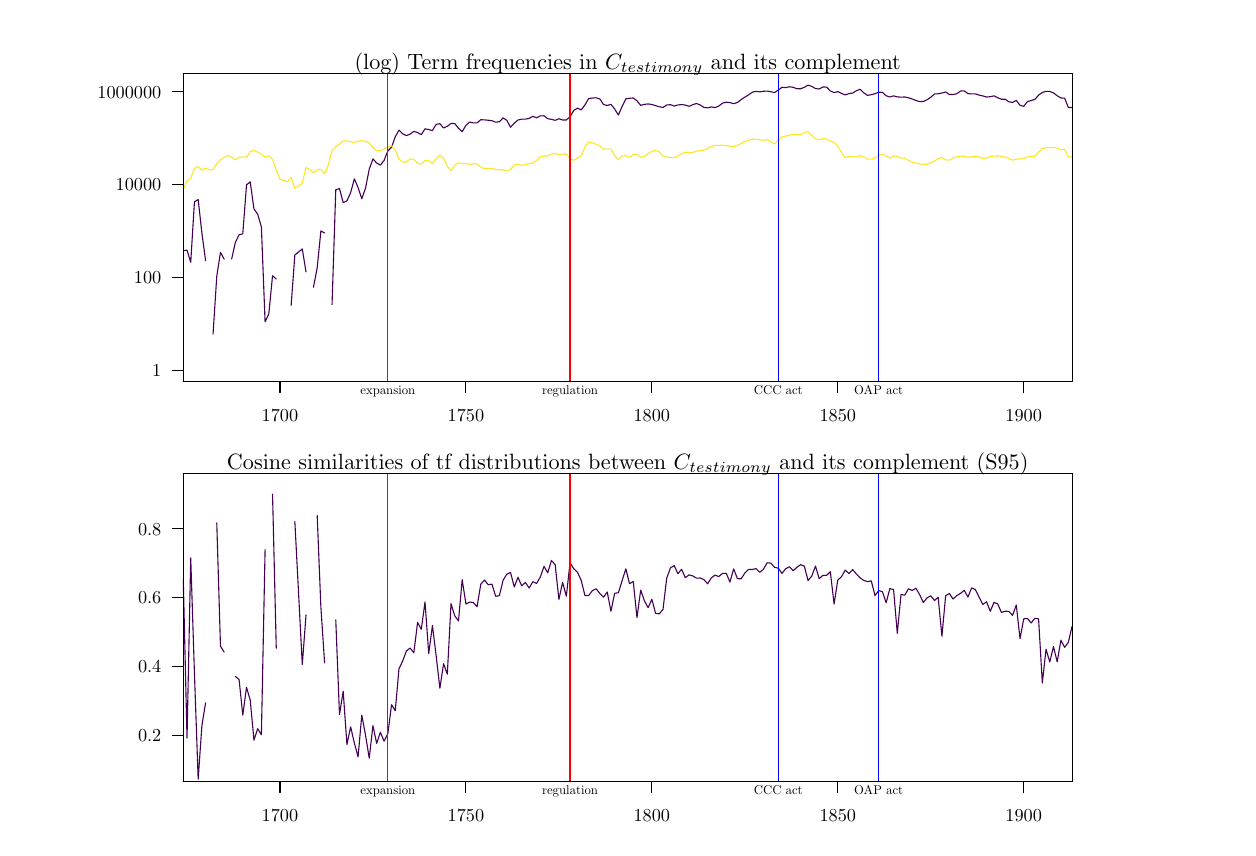
\begin{tikzpicture}[x=1pt,y=1pt]
\definecolor{fillColor}{RGB}{255,255,255}
\path[use as bounding box,fill=fillColor,fill opacity=0.00] (0,0) rectangle (433.62,289.08);
\begin{scope}
\path[clip] (  0.00,  0.00) rectangle (433.62,289.08);
\definecolor{drawColor}{RGB}{0,0,0}

\path[draw=drawColor,line width= 0.4pt,line join=round,line cap=round] ( 91.17,161.17) -- (359.92,161.17);

\path[draw=drawColor,line width= 0.4pt,line join=round,line cap=round] ( 91.17,161.17) -- ( 91.17,157.21);

\path[draw=drawColor,line width= 0.4pt,line join=round,line cap=round] (158.36,161.17) -- (158.36,157.21);

\path[draw=drawColor,line width= 0.4pt,line join=round,line cap=round] (225.54,161.17) -- (225.54,157.21);

\path[draw=drawColor,line width= 0.4pt,line join=round,line cap=round] (292.73,161.17) -- (292.73,157.21);

\path[draw=drawColor,line width= 0.4pt,line join=round,line cap=round] (359.92,161.17) -- (359.92,157.21);

\node[text=drawColor,anchor=base,inner sep=0pt, outer sep=0pt, scale=  0.66] at ( 91.17,146.92) {1700};

\node[text=drawColor,anchor=base,inner sep=0pt, outer sep=0pt, scale=  0.66] at (158.36,146.92) {1750};

\node[text=drawColor,anchor=base,inner sep=0pt, outer sep=0pt, scale=  0.66] at (225.54,146.92) {1800};

\node[text=drawColor,anchor=base,inner sep=0pt, outer sep=0pt, scale=  0.66] at (292.73,146.92) {1850};

\node[text=drawColor,anchor=base,inner sep=0pt, outer sep=0pt, scale=  0.66] at (359.92,146.92) {1900};

\path[draw=drawColor,line width= 0.4pt,line join=round,line cap=round] ( 56.23,165.29) -- ( 56.23,265.88);

\path[draw=drawColor,line width= 0.4pt,line join=round,line cap=round] ( 56.23,165.29) -- ( 52.27,165.29);

\path[draw=drawColor,line width= 0.4pt,line join=round,line cap=round] ( 56.23,198.82) -- ( 52.27,198.82);

\path[draw=drawColor,line width= 0.4pt,line join=round,line cap=round] ( 56.23,232.35) -- ( 52.27,232.35);

\path[draw=drawColor,line width= 0.4pt,line join=round,line cap=round] ( 56.23,265.88) -- ( 52.27,265.88);

\node[text=drawColor,anchor=base east,inner sep=0pt, outer sep=0pt, scale=  0.66] at ( 48.31,163.02) {      1};

\node[text=drawColor,anchor=base east,inner sep=0pt, outer sep=0pt, scale=  0.66] at ( 48.31,196.55) {    100};

\node[text=drawColor,anchor=base east,inner sep=0pt, outer sep=0pt, scale=  0.66] at ( 48.31,230.08) {  10000};

\node[text=drawColor,anchor=base east,inner sep=0pt, outer sep=0pt, scale=  0.66] at ( 48.31,263.61) {1000000};
\definecolor{drawColor}{RGB}{68,1,84}

\path[draw=drawColor,line width= 0.4pt,line join=round,line cap=round] ( 56.23,208.47) --
	( 57.58,208.70) --
	( 58.92,204.31) --
	( 60.26,226.13) --
	( 61.61,226.97) --
	( 62.95,214.89) --
	( 64.29,204.87);

\path[draw=drawColor,line width= 0.4pt,line join=round,line cap=round] ( 66.98,178.34) --
	( 68.33,199.25) --
	( 69.67,207.88) --
	( 71.01,205.41);

\path[draw=drawColor,line width= 0.4pt,line join=round,line cap=round] ( 73.70,205.46) --
	( 75.04,211.46) --
	( 76.39,214.28) --
	( 77.73,214.55) --
	( 79.08,232.29) --
	( 80.42,233.36) --
	( 81.76,223.60) --
	( 83.11,221.67) --
	( 84.45,217.09) --
	( 85.79,182.75) --
	( 87.14,185.70) --
	( 88.48,199.45) --
	( 89.83,198.25);

\path[draw=drawColor,line width= 0.4pt,line join=round,line cap=round] ( 95.20,188.73) --
	( 96.54,206.93) --
	( 99.23,209.11) --
	(100.58,200.82);

\path[draw=drawColor,line width= 0.4pt,line join=round,line cap=round] (103.26,195.28) --
	(104.61,202.27) --
	(105.95,215.64) --
	(107.29,214.88);

\path[draw=drawColor,line width= 0.4pt,line join=round,line cap=round] (109.98,189.01) --
	(111.33,230.50) --
	(112.67,230.92) --
	(114.01,225.89) --
	(115.36,226.48) --
	(116.70,229.46) --
	(118.04,234.46) --
	(119.39,231.32) --
	(120.73,227.26) --
	(122.08,231.09) --
	(123.42,237.94) --
	(124.76,241.66) --
	(126.11,240.16) --
	(127.45,239.41) --
	(128.79,241.11) --
	(130.14,244.54) --
	(131.48,245.87) --
	(132.83,249.66) --
	(134.17,252.07) --
	(135.51,250.75) --
	(136.86,250.06) --
	(138.20,250.62) --
	(139.54,251.61) --
	(140.89,251.17) --
	(142.23,250.41) --
	(143.58,252.54) --
	(144.92,252.25) --
	(146.26,251.89) --
	(147.61,254.13) --
	(148.95,254.38) --
	(150.29,252.84) --
	(151.64,253.44) --
	(152.98,254.50) --
	(154.33,254.40) --
	(155.67,252.73) --
	(157.01,251.51) --
	(158.36,253.76) --
	(159.70,254.96) --
	(161.04,254.67) --
	(162.39,254.69) --
	(163.73,255.82) --
	(165.08,255.76) --
	(166.42,255.62) --
	(167.76,255.46) --
	(169.11,254.93) --
	(170.45,255.09) --
	(171.79,256.47) --
	(173.14,255.60) --
	(174.48,253.10) --
	(175.83,254.56) --
	(177.17,255.70) --
	(178.51,256.01) --
	(179.86,256.02) --
	(181.20,256.31) --
	(182.54,257.04) --
	(183.89,256.50) --
	(185.23,257.18) --
	(186.58,257.24) --
	(187.92,256.21) --
	(189.26,255.93) --
	(190.61,255.59) --
	(191.95,256.16) --
	(193.29,255.71) --
	(194.64,255.72) --
	(195.98,256.90) --
	(197.33,259.18) --
	(198.67,260.01) --
	(200.01,259.36) --
	(201.36,261.16) --
	(202.70,263.50) --
	(204.04,263.63) --
	(205.39,263.74) --
	(206.73,263.34) --
	(208.08,261.30) --
	(209.42,260.98) --
	(210.76,261.36) --
	(212.11,259.65) --
	(213.45,257.51) --
	(214.79,260.62) --
	(216.14,263.36) --
	(217.48,263.55) --
	(218.83,263.69) --
	(220.17,262.65) --
	(221.51,261.01) --
	(222.86,261.37) --
	(224.20,261.51) --
	(225.54,261.32) --
	(226.89,260.90) --
	(228.23,260.49) --
	(229.58,260.26) --
	(230.92,261.14) --
	(232.26,261.25) --
	(233.61,260.77) --
	(234.95,261.14) --
	(236.29,261.30) --
	(237.64,261.11) --
	(238.98,260.65) --
	(240.33,261.26) --
	(241.67,261.68) --
	(243.01,261.14) --
	(244.36,260.26) --
	(245.70,260.09) --
	(247.04,260.45) --
	(248.39,260.21) --
	(249.73,260.76) --
	(251.08,261.80) --
	(252.42,262.14) --
	(253.76,262.01) --
	(255.11,261.61) --
	(256.45,262.02) --
	(257.79,263.07) --
	(259.14,263.96) --
	(260.48,264.78) --
	(261.83,265.74) --
	(263.17,266.08) --
	(264.51,265.88) --
	(265.86,266.10) --
	(267.20,266.16) --
	(268.54,265.93) --
	(269.89,265.61) --
	(271.23,266.51) --
	(272.58,267.54) --
	(273.92,267.42) --
	(275.26,267.73) --
	(276.61,267.51) --
	(277.95,267.03) --
	(279.29,267.01) --
	(280.64,267.53) --
	(281.98,268.32) --
	(283.33,267.86) --
	(284.67,267.08) --
	(286.01,266.92) --
	(287.36,267.65) --
	(288.70,267.60) --
	(290.04,266.22) --
	(291.39,265.62) --
	(292.73,265.97) --
	(294.08,265.32) --
	(295.42,264.77) --
	(296.76,265.27) --
	(298.11,265.44) --
	(299.45,266.31) --
	(300.79,266.82) --
	(302.14,265.52) --
	(303.48,264.61) --
	(304.83,264.86) --
	(306.17,265.20) --
	(307.51,265.76) --
	(308.86,265.69) --
	(310.20,264.46) --
	(311.54,264.04) --
	(312.89,264.44) --
	(314.23,264.06) --
	(315.58,263.97) --
	(316.92,264.03) --
	(318.26,263.75) --
	(319.61,263.29) --
	(320.95,262.78) --
	(322.29,262.36) --
	(323.64,262.41) --
	(324.98,263.03) --
	(326.33,263.92) --
	(327.67,265.12) --
	(329.01,265.19) --
	(330.36,265.47) --
	(331.70,265.83) --
	(333.04,264.94) --
	(334.39,264.91) --
	(335.73,265.21) --
	(337.08,266.18) --
	(338.42,266.25) --
	(339.76,265.25) --
	(341.11,265.13) --
	(342.45,265.17) --
	(343.79,264.71) --
	(345.14,264.41) --
	(346.48,264.01) --
	(347.83,264.13) --
	(349.17,264.44) --
	(350.51,263.77) --
	(351.86,263.20) --
	(353.20,263.23) --
	(354.54,262.29) --
	(355.89,262.07) --
	(357.23,262.82) --
	(358.58,261.03) --
	(359.92,260.65) --
	(361.26,262.35) --
	(362.61,262.74) --
	(363.95,263.16) --
	(365.29,264.71) --
	(366.64,265.65) --
	(367.98,266.08) --
	(369.33,266.03) --
	(370.67,265.51) --
	(372.01,264.49) --
	(373.36,263.68) --
	(374.70,263.60) --
	(376.04,260.24) --
	(377.39,260.24);
\definecolor{drawColor}{RGB}{253,231,37}

\path[draw=drawColor,line width= 0.4pt,line join=round,line cap=round] ( 56.23,230.74) --
	( 57.58,233.72) --
	( 58.92,234.67) --
	( 60.26,238.25) --
	( 61.61,238.91) --
	( 62.95,237.61) --
	( 64.29,238.33) --
	( 65.64,237.70) --
	( 66.98,237.77) --
	( 68.33,239.88) --
	( 69.67,241.41) --
	( 71.01,242.11) --
	( 72.36,242.96) --
	( 73.70,242.36) --
	( 75.04,241.31) --
	( 76.39,242.20) --
	( 77.73,242.41) --
	( 79.08,242.24) --
	( 80.42,244.32) --
	( 81.76,244.75) --
	( 83.11,244.08) --
	( 84.45,243.49) --
	( 85.79,242.24) --
	( 87.14,242.79) --
	( 88.48,241.48) --
	( 89.83,237.52) --
	( 91.17,234.29) --
	( 93.86,233.34) --
	( 95.20,234.93) --
	( 96.54,231.05) --
	( 99.23,232.86) --
	(100.58,238.58) --
	(101.92,237.86) --
	(103.26,236.69) --
	(104.61,237.67) --
	(105.95,237.83) --
	(107.29,236.21) --
	(108.64,239.46) --
	(109.98,244.82) --
	(111.33,246.06) --
	(112.67,247.04) --
	(114.01,248.18) --
	(115.36,248.15) --
	(116.70,247.91) --
	(118.04,247.55) --
	(119.39,248.03) --
	(120.73,248.26) --
	(122.08,248.04) --
	(123.42,247.34) --
	(124.76,245.78) --
	(126.11,244.66) --
	(127.45,244.56) --
	(128.79,245.22) --
	(130.14,245.91) --
	(131.48,246.48) --
	(132.83,244.79) --
	(134.17,241.62) --
	(135.51,240.54) --
	(136.86,240.52) --
	(138.20,241.66) --
	(139.54,241.47) --
	(140.89,240.12) --
	(142.23,239.74) --
	(143.58,241.02) --
	(144.92,241.10) --
	(146.26,239.93) --
	(147.61,241.61) --
	(148.95,243.06) --
	(150.29,241.84) --
	(151.64,239.00) --
	(152.98,237.43) --
	(154.33,239.44) --
	(155.67,240.25) --
	(157.01,239.92) --
	(158.36,239.96) --
	(159.70,239.67) --
	(161.04,239.99) --
	(162.39,239.77) --
	(163.73,238.76) --
	(165.08,238.18) --
	(166.42,238.25) --
	(167.76,238.24) --
	(169.11,237.86) --
	(170.45,237.71) --
	(171.79,237.76) --
	(173.14,237.27) --
	(174.48,237.84) --
	(175.83,239.51) --
	(177.17,239.70) --
	(178.51,239.32) --
	(179.86,239.58) --
	(181.20,239.95) --
	(182.54,240.22) --
	(183.89,241.03) --
	(185.23,242.40) --
	(186.58,242.71) --
	(187.92,242.71) --
	(189.26,243.38) --
	(190.61,243.59) --
	(191.95,243.21) --
	(193.29,243.41) --
	(194.64,243.42) --
	(195.98,241.70) --
	(197.33,241.17) --
	(198.67,241.93) --
	(200.01,242.80) --
	(201.36,245.95) --
	(202.70,247.85) --
	(204.04,247.47) --
	(205.39,246.94) --
	(206.73,246.38) --
	(208.08,245.22) --
	(209.42,245.20) --
	(210.76,245.19) --
	(212.11,242.82) --
	(213.45,241.37) --
	(214.79,242.69) --
	(216.14,242.84) --
	(217.48,242.17) --
	(218.83,243.29) --
	(220.17,243.35) --
	(221.51,242.19) --
	(222.86,242.56) --
	(224.20,243.55) --
	(225.54,244.40) --
	(226.89,244.73) --
	(228.23,244.17) --
	(229.58,242.61) --
	(230.92,242.29) --
	(232.26,242.23) --
	(233.61,242.13) --
	(234.95,242.66) --
	(236.29,243.50) --
	(237.64,244.10) --
	(238.98,243.88) --
	(240.33,243.98) --
	(241.67,244.46) --
	(243.01,244.66) --
	(244.36,244.87) --
	(245.70,245.41) --
	(247.04,246.17) --
	(248.39,246.50) --
	(249.73,246.55) --
	(251.08,246.65) --
	(252.42,246.48) --
	(253.76,246.26) --
	(255.11,246.12) --
	(256.45,246.54) --
	(257.79,247.22) --
	(259.14,247.88) --
	(260.48,248.47) --
	(261.83,248.74) --
	(263.17,248.80) --
	(264.51,248.57) --
	(265.86,248.37) --
	(267.20,248.64) --
	(268.54,247.82) --
	(269.89,247.05) --
	(271.23,248.53) --
	(272.58,249.59) --
	(273.92,249.90) --
	(275.26,250.29) --
	(276.61,250.53) --
	(277.95,250.38) --
	(279.29,250.43) --
	(280.64,251.21) --
	(281.98,251.45) --
	(283.33,250.19) --
	(284.67,248.94) --
	(286.01,248.57) --
	(287.36,248.98) --
	(288.70,248.87) --
	(290.04,248.11) --
	(291.39,247.52) --
	(292.73,246.29) --
	(294.08,243.95) --
	(295.42,242.05) --
	(296.76,242.64) --
	(298.11,242.43) --
	(299.45,242.39) --
	(300.79,242.84) --
	(302.14,242.32) --
	(303.48,241.59) --
	(304.83,241.57) --
	(306.17,242.00) --
	(307.51,242.89) --
	(308.86,243.41) --
	(310.20,242.59) --
	(311.54,241.96) --
	(312.89,242.78) --
	(314.23,242.52) --
	(315.58,241.91) --
	(316.92,241.94) --
	(318.26,241.09) --
	(319.61,240.51) --
	(320.95,240.19) --
	(322.29,239.80) --
	(323.64,239.74) --
	(324.98,239.74) --
	(326.33,240.32) --
	(327.67,240.87) --
	(329.01,241.79) --
	(330.36,242.13) --
	(331.70,241.32) --
	(333.04,241.21) --
	(334.39,241.98) --
	(335.73,242.42) --
	(337.08,242.70) --
	(338.42,242.56) --
	(339.76,242.22) --
	(341.11,242.44) --
	(342.45,242.59) --
	(343.79,242.48) --
	(345.14,241.86) --
	(346.48,241.95) --
	(347.83,242.56) --
	(349.17,242.66) --
	(350.51,242.72) --
	(351.86,242.60) --
	(353.20,242.30) --
	(354.54,241.73) --
	(355.89,241.19) --
	(357.23,241.65) --
	(358.58,241.59) --
	(359.92,241.75) --
	(361.26,242.36) --
	(362.61,242.56) --
	(363.95,242.64) --
	(365.29,244.13) --
	(366.64,245.34) --
	(367.98,245.71) --
	(369.33,245.71) --
	(370.67,245.81) --
	(372.01,245.60) --
	(373.36,244.93) --
	(374.70,245.10) --
	(376.04,242.33) --
	(377.39,242.33);
\definecolor{drawColor}{RGB}{0,0,0}

\node[text=drawColor,anchor=base,inner sep=0pt, outer sep=0pt, scale=  0.80] at (216.81,274.03) {(log) Term frequencies in $C_{testimony}$ and its complement};
\end{scope}
\begin{scope}
\path[clip] ( 56.23,161.17) rectangle (377.39,272.45);
\definecolor{drawColor}{RGB}{255,0,0}

\path[draw=drawColor,line width= 0.4pt,line join=round,line cap=round] (130.14,161.17) -- (130.14,272.45);

\path[draw=drawColor,line width= 0.4pt,line join=round,line cap=round] (195.98,161.17) -- (195.98,272.45);
\definecolor{drawColor}{RGB}{0,0,255}

\path[draw=drawColor,line width= 0.4pt,line join=round,line cap=round] (271.23,161.17) -- (271.23,272.45);

\path[draw=drawColor,line width= 0.4pt,line join=round,line cap=round] (307.51,161.17) -- (307.51,272.45);
\end{scope}
\begin{scope}
\path[clip] (  0.00,  0.00) rectangle (433.62,289.08);
\definecolor{drawColor}{RGB}{0,0,0}

\node[text=drawColor,anchor=base,inner sep=0pt, outer sep=0pt, scale=  0.46] at (130.14,156.42) {expansion};

\node[text=drawColor,anchor=base,inner sep=0pt, outer sep=0pt, scale=  0.46] at (195.98,156.42) {regulation};

\node[text=drawColor,anchor=base,inner sep=0pt, outer sep=0pt, scale=  0.46] at (271.23,156.42) {CCC act};

\node[text=drawColor,anchor=base,inner sep=0pt, outer sep=0pt, scale=  0.46] at (307.51,156.42) {OAP act};

\path[draw=drawColor,line width= 0.4pt,line join=round,line cap=round] ( 56.23,161.17) --
	(377.39,161.17) --
	(377.39,272.45) --
	( 56.23,272.45) --
	( 56.23,161.17);
\end{scope}
\begin{scope}
\path[clip] (  0.00,  0.00) rectangle (433.62,289.08);
\definecolor{drawColor}{RGB}{0,0,0}

\path[draw=drawColor,line width= 0.4pt,line join=round,line cap=round] ( 91.17, 16.63) -- (359.92, 16.63);

\path[draw=drawColor,line width= 0.4pt,line join=round,line cap=round] ( 91.17, 16.63) -- ( 91.17, 12.67);

\path[draw=drawColor,line width= 0.4pt,line join=round,line cap=round] (158.36, 16.63) -- (158.36, 12.67);

\path[draw=drawColor,line width= 0.4pt,line join=round,line cap=round] (225.54, 16.63) -- (225.54, 12.67);

\path[draw=drawColor,line width= 0.4pt,line join=round,line cap=round] (292.73, 16.63) -- (292.73, 12.67);

\path[draw=drawColor,line width= 0.4pt,line join=round,line cap=round] (359.92, 16.63) -- (359.92, 12.67);

\node[text=drawColor,anchor=base,inner sep=0pt, outer sep=0pt, scale=  0.66] at ( 91.17,  2.38) {1700};

\node[text=drawColor,anchor=base,inner sep=0pt, outer sep=0pt, scale=  0.66] at (158.36,  2.38) {1750};

\node[text=drawColor,anchor=base,inner sep=0pt, outer sep=0pt, scale=  0.66] at (225.54,  2.38) {1800};

\node[text=drawColor,anchor=base,inner sep=0pt, outer sep=0pt, scale=  0.66] at (292.73,  2.38) {1850};

\node[text=drawColor,anchor=base,inner sep=0pt, outer sep=0pt, scale=  0.66] at (359.92,  2.38) {1900};

\path[draw=drawColor,line width= 0.4pt,line join=round,line cap=round] ( 56.23, 33.27) -- ( 56.23,108.01);

\path[draw=drawColor,line width= 0.4pt,line join=round,line cap=round] ( 56.23, 33.27) -- ( 52.27, 33.27);

\path[draw=drawColor,line width= 0.4pt,line join=round,line cap=round] ( 56.23, 58.19) -- ( 52.27, 58.19);

\path[draw=drawColor,line width= 0.4pt,line join=round,line cap=round] ( 56.23, 83.10) -- ( 52.27, 83.10);

\path[draw=drawColor,line width= 0.4pt,line join=round,line cap=round] ( 56.23,108.01) -- ( 52.27,108.01);

\node[text=drawColor,anchor=base east,inner sep=0pt, outer sep=0pt, scale=  0.66] at ( 48.31, 31.00) {0.2};

\node[text=drawColor,anchor=base east,inner sep=0pt, outer sep=0pt, scale=  0.66] at ( 48.31, 55.91) {0.4};

\node[text=drawColor,anchor=base east,inner sep=0pt, outer sep=0pt, scale=  0.66] at ( 48.31, 80.83) {0.6};

\node[text=drawColor,anchor=base east,inner sep=0pt, outer sep=0pt, scale=  0.66] at ( 48.31,105.74) {0.8};

\path[draw=drawColor,line width= 0.4pt,line join=round,line cap=round] ( 56.23, 16.63) --
	(377.39, 16.63) --
	(377.39,127.91) --
	( 56.23,127.91) --
	( 56.23, 16.63);
\definecolor{drawColor}{RGB}{68,1,84}

\path[draw=drawColor,line width= 0.4pt,line join=round,line cap=round] ( 56.23, 89.55) --
	( 57.58, 32.35) --
	( 58.92, 97.49) --
	( 60.26, 55.75) --
	( 61.61, 17.50) --
	( 62.95, 36.85) --
	( 64.29, 45.09);

\path[draw=drawColor,line width= 0.4pt,line join=round,line cap=round] ( 68.33,110.14) --
	( 69.67, 65.54) --
	( 71.01, 63.45);

\path[draw=drawColor,line width= 0.4pt,line join=round,line cap=round] ( 75.04, 54.66) --
	( 76.39, 53.55) --
	( 77.73, 40.66) --
	( 79.08, 50.72) --
	( 80.42, 46.08) --
	( 81.76, 31.61) --
	( 83.11, 35.77) --
	( 84.45, 33.58) --
	( 85.79,100.51);

\path[draw=drawColor,line width= 0.4pt,line join=round,line cap=round] ( 88.48,120.53) --
	( 89.83, 64.85);

\path[draw=drawColor,line width= 0.4pt,line join=round,line cap=round] ( 96.54,110.66) --
	( 99.23, 58.94) --
	(100.58, 76.86);

\path[draw=drawColor,line width= 0.4pt,line join=round,line cap=round] (104.61,112.85) --
	(105.95, 79.69) --
	(107.29, 59.56);

\path[draw=drawColor,line width= 0.4pt,line join=round,line cap=round] (111.33, 75.06) --
	(112.67, 40.91) --
	(114.01, 49.29) --
	(115.36, 30.05) --
	(116.70, 36.44) --
	(118.04, 30.60) --
	(119.39, 25.59) --
	(120.73, 40.66) --
	(122.08, 33.47) --
	(123.42, 25.13) --
	(124.76, 36.87) --
	(126.11, 30.44) --
	(127.45, 34.47) --
	(128.79, 31.26) --
	(130.14, 33.92) --
	(131.48, 44.42) --
	(132.83, 42.26) --
	(134.17, 57.43) --
	(135.51, 60.22) --
	(136.86, 63.86) --
	(138.20, 64.90) --
	(139.54, 63.19) --
	(140.89, 74.15) --
	(142.23, 71.69) --
	(143.58, 81.59) --
	(144.92, 62.89) --
	(146.26, 73.07) --
	(147.61, 62.03) --
	(148.95, 50.39) --
	(150.29, 59.26) --
	(151.64, 55.45) --
	(152.98, 80.95) --
	(154.33, 76.52) --
	(155.67, 74.70) --
	(157.01, 89.62) --
	(158.36, 80.82) --
	(159.70, 81.52) --
	(161.04, 81.35) --
	(162.39, 79.84) --
	(163.73, 87.99) --
	(165.08, 89.50) --
	(166.42, 87.77) --
	(167.76, 88.01) --
	(169.11, 83.61) --
	(170.45, 83.82) --
	(171.79, 89.41) --
	(173.14, 91.61) --
	(174.48, 92.21) --
	(175.83, 86.98) --
	(177.17, 90.49) --
	(178.51, 87.36) --
	(179.86, 88.62) --
	(181.20, 86.60) --
	(182.54, 88.89) --
	(183.89, 88.24) --
	(185.23, 90.55) --
	(186.58, 94.42) --
	(187.92, 92.09) --
	(189.26, 96.55) --
	(190.61, 95.06) --
	(191.95, 82.48) --
	(193.29, 88.63) --
	(194.64, 83.64) --
	(195.98, 95.77) --
	(197.33, 93.55) --
	(198.67, 92.27) --
	(200.01, 89.41) --
	(201.36, 83.90) --
	(202.70, 83.86) --
	(204.04, 85.64) --
	(205.39, 86.32) --
	(206.73, 84.67) --
	(208.08, 83.29) --
	(209.42, 85.16) --
	(210.76, 78.22) --
	(212.11, 84.71) --
	(213.45, 84.89) --
	(214.79, 89.21) --
	(216.14, 93.55) --
	(217.48, 88.15) --
	(218.83, 88.96) --
	(220.17, 75.91) --
	(221.51, 85.86) --
	(222.86, 81.97) --
	(224.20, 79.51) --
	(225.54, 82.53) --
	(226.89, 77.45) --
	(228.23, 77.26) --
	(229.58, 78.90) --
	(230.92, 90.16) --
	(232.26, 93.86) --
	(233.61, 94.71) --
	(234.95, 91.78) --
	(236.29, 93.36) --
	(237.64, 90.32) --
	(238.98, 91.36) --
	(240.33, 90.97) --
	(241.67, 90.15) --
	(243.01, 90.22) --
	(244.36, 89.64) --
	(245.70, 88.13) --
	(247.04, 90.28) --
	(248.39, 91.25) --
	(249.73, 90.73) --
	(251.08, 91.89) --
	(252.42, 91.92) --
	(253.76, 88.76) --
	(255.11, 93.53) --
	(256.45, 89.99) --
	(257.79, 89.93) --
	(259.14, 91.98) --
	(260.48, 93.32) --
	(261.83, 93.29) --
	(263.17, 93.62) --
	(264.51, 92.27) --
	(265.86, 93.37) --
	(267.20, 95.72) --
	(268.54, 95.60) --
	(269.89, 94.07) --
	(271.23, 93.77) --
	(272.58, 91.90) --
	(273.92, 93.58) --
	(275.26, 94.28) --
	(276.61, 92.85) --
	(277.95, 94.10) --
	(279.29, 95.03) --
	(280.64, 94.51) --
	(281.98, 89.31) --
	(283.33, 90.91) --
	(284.67, 94.53) --
	(286.01, 89.99) --
	(287.36, 91.17) --
	(288.70, 91.20) --
	(290.04, 92.49) --
	(291.39, 80.81) --
	(292.73, 89.47) --
	(294.08, 90.69) --
	(295.42, 93.08) --
	(296.76, 91.82) --
	(298.11, 93.26) --
	(299.45, 91.66) --
	(300.79, 90.27) --
	(302.14, 89.34) --
	(303.48, 88.91) --
	(304.83, 89.19) --
	(306.17, 83.86) --
	(307.51, 85.67) --
	(308.86, 85.26) --
	(310.20, 81.24) --
	(311.54, 86.41) --
	(312.89, 86.03) --
	(314.23, 70.21) --
	(315.58, 84.27) --
	(316.92, 84.00) --
	(318.26, 86.32) --
	(319.61, 85.71) --
	(320.95, 86.53) --
	(322.29, 84.24) --
	(323.64, 81.38) --
	(324.98, 83.03) --
	(326.33, 83.80) --
	(327.67, 82.08) --
	(329.01, 83.25) --
	(330.36, 69.14) --
	(331.70, 83.79) --
	(333.04, 84.63) --
	(334.39, 82.62) --
	(335.73, 83.85) --
	(337.08, 84.66) --
	(338.42, 85.75) --
	(339.76, 83.32) --
	(341.11, 86.66) --
	(342.45, 86.02) --
	(343.79, 83.34) --
	(345.14, 80.62) --
	(346.48, 81.65) --
	(347.83, 78.19) --
	(349.17, 81.41) --
	(350.51, 80.89) --
	(351.86, 77.78) --
	(353.20, 78.21) --
	(354.54, 78.16) --
	(355.89, 76.69) --
	(357.23, 80.48) --
	(358.58, 68.32) --
	(359.92, 75.46) --
	(361.26, 75.61) --
	(362.61, 73.97) --
	(363.95, 75.64) --
	(365.29, 75.44) --
	(366.64, 52.28) --
	(367.98, 64.48) --
	(369.33, 59.88) --
	(370.67, 65.45) --
	(372.01, 59.92) --
	(373.36, 67.74) --
	(374.70, 65.15) --
	(376.04, 66.98) --
	(377.39, 72.78);
\definecolor{drawColor}{RGB}{0,0,0}

\node[text=drawColor,anchor=base,inner sep=0pt, outer sep=0pt, scale=  0.80] at (216.81,129.49) {Cosine similarities of tf distributions between $C_{testimony}$ and its complement (S95)};
\end{scope}
\begin{scope}
\path[clip] ( 56.23, 16.63) rectangle (377.39,127.91);
\definecolor{drawColor}{RGB}{255,0,0}

\path[draw=drawColor,line width= 0.4pt,line join=round,line cap=round] (130.14, 16.63) -- (130.14,127.91);

\path[draw=drawColor,line width= 0.4pt,line join=round,line cap=round] (195.98, 16.63) -- (195.98,127.91);
\definecolor{drawColor}{RGB}{0,0,255}

\path[draw=drawColor,line width= 0.4pt,line join=round,line cap=round] (271.23, 16.63) -- (271.23,127.91);

\path[draw=drawColor,line width= 0.4pt,line join=round,line cap=round] (307.51, 16.63) -- (307.51,127.91);
\end{scope}
\begin{scope}
\path[clip] (  0.00,  0.00) rectangle (433.62,289.08);
\definecolor{drawColor}{RGB}{0,0,0}

\node[text=drawColor,anchor=base,inner sep=0pt, outer sep=0pt, scale=  0.46] at (130.14, 11.88) {expansion};

\node[text=drawColor,anchor=base,inner sep=0pt, outer sep=0pt, scale=  0.46] at (195.98, 11.88) {regulation};

\node[text=drawColor,anchor=base,inner sep=0pt, outer sep=0pt, scale=  0.46] at (271.23, 11.88) {CCC act};

\node[text=drawColor,anchor=base,inner sep=0pt, outer sep=0pt, scale=  0.46] at (307.51, 11.88) {OAP act};

\path[draw=drawColor,line width= 0.4pt,line join=round,line cap=round] ( 56.23, 16.63) --
	(377.39, 16.63) --
	(377.39,127.91) --
	( 56.23,127.91) --
	( 56.23, 16.63);
\end{scope}
\end{tikzpicture}

    \caption[$C_{testiomony}$ and its complement]{
        Longitudinal comparison between $C_{testimony}$ and its complement for every year in the POB
    }
    \label{fig:testimony_long}
\end{figure}

As can be seen from this result, the construction of $C_{testimony}$ appears as a reasonable approximation of the purported direct-speech content in the POB, and the general trend corresponds to what we would expect given the knowledge about the production of the POB that we have available from traditional historical research.

The upper panel in this figure provides ample evidence that $C_{testimony}$ actually captures direct speech, as the point in time in which its total term frequency overtakes that of its complement corresponds \emph{exactly} to the point in time at which traditional historical research tells us that the POB began to include witness testimony more systematically.

The lower panel, on the other hand, confirms what we would expect about the evolution of the POB given its progressive transformation from edited selection of entertaining trials to faithful record of the dealings at court: the first period of the POB shows an erratic trend, mainly determined by the low frequency counts obtained from the pamphlet-style surviving issues from the late 17th century, but as we move into the 18th century we appreciate a decided trend of stabilisation though which $C_{testimony}$ becomes increasingly distinct from its complement, indicating a progressive separation between those segments of the trial accounts corresponding to legal paraphernalia and those assumed to contain witness testimony from our naive detection strategy.

In addition to this longitudinal comparison across samples, we can also produce the same self-similarity matrices used in the analysis of the SOTU corpus in order to look at the evolution of each corpus sample on its own.
\autoref{fig:testimony_inner} shows the raw cosine similarity (i.e. not inverted) for each sample side by side.

\begin{figure}
    \centerfloat
    % Created by tikzDevice version 0.12 on 2018-08-02 17:34:01
% !TEX encoding = UTF-8 Unicode
\begin{tikzpicture}[x=1pt,y=1pt]
\definecolor{fillColor}{RGB}{255,255,255}
\path[use as bounding box,fill=fillColor,fill opacity=0.00] (0,0) rectangle (433.62,144.54);
\begin{scope}
\path[clip] (  0.00,  0.00) rectangle (433.62,144.54);
\node[inner sep=0pt,outer sep=0pt,anchor=south west,rotate=  0.00] at ( 88.90,  16.63) {
	\pgfimage[width=111.28pt,height=111.28pt,interpolate=true]{c2_testimony_fig2_ras1}};
\definecolor{drawColor}{RGB}{0,0,0}

\node[text=drawColor,anchor=base,inner sep=0pt, outer sep=0pt, scale=  0.80] at (144.54,129.49) {$C_{testimony}$};

\path[draw=drawColor,line width= 0.4pt,line join=round,line cap=round] (101.01, 16.63) -- (194.13, 16.63);

\path[draw=drawColor,line width= 0.4pt,line join=round,line cap=round] (101.01, 16.63) -- (101.01, 12.67);

\path[draw=drawColor,line width= 0.4pt,line join=round,line cap=round] (124.29, 16.63) -- (124.29, 12.67);

\path[draw=drawColor,line width= 0.4pt,line join=round,line cap=round] (147.57, 16.63) -- (147.57, 12.67);

\path[draw=drawColor,line width= 0.4pt,line join=round,line cap=round] (170.85, 16.63) -- (170.85, 12.67);

\path[draw=drawColor,line width= 0.4pt,line join=round,line cap=round] (194.13, 16.63) -- (194.13, 12.67);

\node[text=drawColor,anchor=base,inner sep=0pt, outer sep=0pt, scale=  0.66] at (101.01,  2.38) {1700};

\node[text=drawColor,anchor=base,inner sep=0pt, outer sep=0pt, scale=  0.66] at (124.29,  2.38) {1750};

\node[text=drawColor,anchor=base,inner sep=0pt, outer sep=0pt, scale=  0.66] at (147.57,  2.38) {1800};

\node[text=drawColor,anchor=base,inner sep=0pt, outer sep=0pt, scale=  0.66] at (170.85,  2.38) {1850};

\node[text=drawColor,anchor=base,inner sep=0pt, outer sep=0pt, scale=  0.66] at (194.13,  2.38) {1900};
\end{scope}
\begin{scope}
\path[clip] ( 88.90, 16.63) rectangle (200.18,127.91);
\definecolor{drawColor}{RGB}{255,0,0}

\path[draw=drawColor,line width= 0.4pt,line join=round,line cap=round] (114.51, 16.63) -- (114.51,127.91);

\path[draw=drawColor,line width= 0.4pt,line join=round,line cap=round] (137.32, 16.63) -- (137.32,127.91);
\definecolor{drawColor}{RGB}{0,0,255}

\path[draw=drawColor,line width= 0.4pt,line join=round,line cap=round] (163.40, 16.63) -- (163.40,127.91);

\path[draw=drawColor,line width= 0.4pt,line join=round,line cap=round] (175.97, 16.63) -- (175.97,127.91);
\end{scope}
\begin{scope}
\path[clip] (  0.00,  0.00) rectangle (433.62,144.54);
\definecolor{drawColor}{RGB}{0,0,0}

\path[draw=drawColor,line width= 0.4pt,line join=round,line cap=round] ( 88.90, 16.63) --
	(200.18, 16.63) --
	(200.18,127.91) --
	( 88.90,127.91) --
	( 88.90, 16.63);
\end{scope}
\begin{scope}
\path[clip] (  0.00,  0.00) rectangle (433.62,144.54);
\node[inner sep=0pt,outer sep=0pt,anchor=south west,rotate=  0.00] at (233.44,  16.63) {
	\pgfimage[width=111.28pt,height=111.28pt,interpolate=true]{c2_testimony_fig2_ras2}};
\definecolor{drawColor}{RGB}{0,0,0}

\node[text=drawColor,anchor=base,inner sep=0pt, outer sep=0pt, scale=  0.80] at (289.08,129.49) {$\sim C_{testimony}$};

\path[draw=drawColor,line width= 0.4pt,line join=round,line cap=round] (245.55, 16.63) -- (338.67, 16.63);

\path[draw=drawColor,line width= 0.4pt,line join=round,line cap=round] (245.55, 16.63) -- (245.55, 12.67);

\path[draw=drawColor,line width= 0.4pt,line join=round,line cap=round] (268.83, 16.63) -- (268.83, 12.67);

\path[draw=drawColor,line width= 0.4pt,line join=round,line cap=round] (292.11, 16.63) -- (292.11, 12.67);

\path[draw=drawColor,line width= 0.4pt,line join=round,line cap=round] (315.39, 16.63) -- (315.39, 12.67);

\path[draw=drawColor,line width= 0.4pt,line join=round,line cap=round] (338.67, 16.63) -- (338.67, 12.67);

\node[text=drawColor,anchor=base,inner sep=0pt, outer sep=0pt, scale=  0.66] at (245.55,  2.38) {1700};

\node[text=drawColor,anchor=base,inner sep=0pt, outer sep=0pt, scale=  0.66] at (268.83,  2.38) {1750};

\node[text=drawColor,anchor=base,inner sep=0pt, outer sep=0pt, scale=  0.66] at (292.11,  2.38) {1800};

\node[text=drawColor,anchor=base,inner sep=0pt, outer sep=0pt, scale=  0.66] at (315.39,  2.38) {1850};

\node[text=drawColor,anchor=base,inner sep=0pt, outer sep=0pt, scale=  0.66] at (338.67,  2.38) {1900};
\end{scope}
\begin{scope}
\path[clip] (233.44, 16.63) rectangle (344.72,127.91);
\definecolor{drawColor}{RGB}{255,0,0}

\path[draw=drawColor,line width= 0.4pt,line join=round,line cap=round] (259.05, 16.63) -- (259.05,127.91);

\path[draw=drawColor,line width= 0.4pt,line join=round,line cap=round] (281.86, 16.63) -- (281.86,127.91);
\definecolor{drawColor}{RGB}{0,0,255}

\path[draw=drawColor,line width= 0.4pt,line join=round,line cap=round] (307.94, 16.63) -- (307.94,127.91);

\path[draw=drawColor,line width= 0.4pt,line join=round,line cap=round] (320.51, 16.63) -- (320.51,127.91);
\end{scope}
\begin{scope}
\path[clip] (  0.00,  0.00) rectangle (433.62,144.54);
\definecolor{drawColor}{RGB}{0,0,0}

\path[draw=drawColor,line width= 0.4pt,line join=round,line cap=round] (233.44, 16.63) --
	(344.72, 16.63) --
	(344.72,127.91) --
	(233.44,127.91) --
	(233.44, 16.63);
\end{scope}
\end{tikzpicture}

    \caption[Cosine similarities for $C_{testimony}$ and complement]{
        Cosine self-similarity for $C_{testimony}$ and its complement for every year in the POB
    }
    \label{fig:testimony_inner}
\end{figure}

As can be expected, we again observe the same general pattern: $C_{tetimony}$ initially shows a rather low level of self-similarity from year to year, reflecting its low occurrence in that region of the corpus, but also suggesting that whatever is contained in it for those early years is dominated by particular idiosyncrasies in language use, possibly because of a large role of the individual author in the composition of ``entertaining'' narratives of the most salacious trials.
But starting in 1730, the content of $C_{testimony}$ becomes surprisingly stable.
Again, this corresponds \emph{exactly} to the point in time in which the POB is supposed to have begun to include witness testimony in earnest, a fact that is strongly supported by this entirely endogenous indicator.
Comparatively, this level of self-similarity (i.e. stability) is not achieved by any other split of the POB, not even the full corpus without any selection procedure, either when looking at the term vectors for the full lexicon, a version containing only lexicals or a version containing only functionals.

$C_{testimony}$'s complement on the other hand, shows a much more happened history in which it is not easy to discern a general trend.
There are clearly marked periods of substantial self-similarity in this region of the corpus, but it is not easy to interpret their meaning, particularly since they do not seem to align with either of the moments at which we know that administrative change was introduced, from which one could expect to observe some associated variations in the general usage patterns of the legal paraphernalia that we expect to make up most of $C_{testimony}$'s complement.

\citet{klingenstein2014} carry out their analysis using a completely different strategy, both for construction of the term vectors and for the choice of a similarity measure.
First, they do not use cosine similarities as measure of comparison, but the Jensen-Shannon divergence measure.
In the context of the discussion in \autoref{app:simdiv}, this belongs to the ``probabilistic'' family of similarity functions, which treat the term-vector as a probability distribution and asses the amount of information loss in predictions about one of the distributions from information provided by the other.
The JSD in particular is a symmetrised, reflective modification of the Kullback-Leibler divergence: it is the average KL divergence of both distributions from the linear combination of both\footnote{
    $JSD_{P,Q} = \frac{1}{2} KL(P,M) + KL(Q,M) : M = \frac{1}{2} P + Q$.
    See \autoref{app:simdiv} for details.
}.

Second, since the JSD produces singularities on $0$, in the original exercise they apply a coarsening procedure based on the synonym sets from Roget's Thesaurus, such that the term-vectors are not built over the elements in the lexicon directly, but over the frequencies of the synonym heads into which each term in the POB lexicon is classified by the thesaurus.
This produces denser vectors of dimensionality equal to the cardinality of the thesaurus head-set: $1041$.
It also operates as a censoring over the entire lexical sample, as not every term in the POB appears in Roget's.
In the original work, based on the OBC edition of the POB, this censoring effect is not so large because the OBC lexicon is much smaller than the entire POB lexicon and most of the $\sim 15,000$ terms in the OBC do appear in the thesaurus.
This is not the case for the OBO edition of the POB with its $77,610$ entries, though the final effect is more or less comparable to the information loss from using the $S95$ sample in terms of total token-stream coverage.
There is a critical difference, however: using a thesaurus-based coarsening procedure imposes an exogenous structure over the empirical distributions, introducing an additional confounding factor, as using the aggregated head counts makes it impossible to ascertain if any observed trends are due to changes in the the social context that produces the observed usage patterns, or to changes on the meanings of words across different points in time, though this is a general limitation of term-frequency based comparisons; the introduction of additional structure just adds a second level of confusion\footnote{
    \label{foot:semstat}
    The comparison of term frequencies, with or without the imposition of an exogenous structure, relies on the assumption that a given word has semantic stability across the comparison, i.e. it ``means the same thing'', as frequency based comparisons offer no insight into the relationship between different words which the distributional hypothesis suggests to be determinant of its meaning.
    Less \term{kill} may mean less actual killing, or it could mean that actual killings stop being called \term{kill} and start to be referred to as \term{murder}, etc.
    The imposition of external structure adds on to this assumption, as it is based on the idea that the imposed structure (in this case, mr. Roget's beautiful attempt at categorising all of human knowledge in the second part of the nineteenth century) is equally valid at all points of the comparison.
}.

\begin{figure}
    \centerfloat
    % Created by tikzDevice version 0.12 on 2018-08-02 17:29:57
% !TEX encoding = UTF-8 Unicode
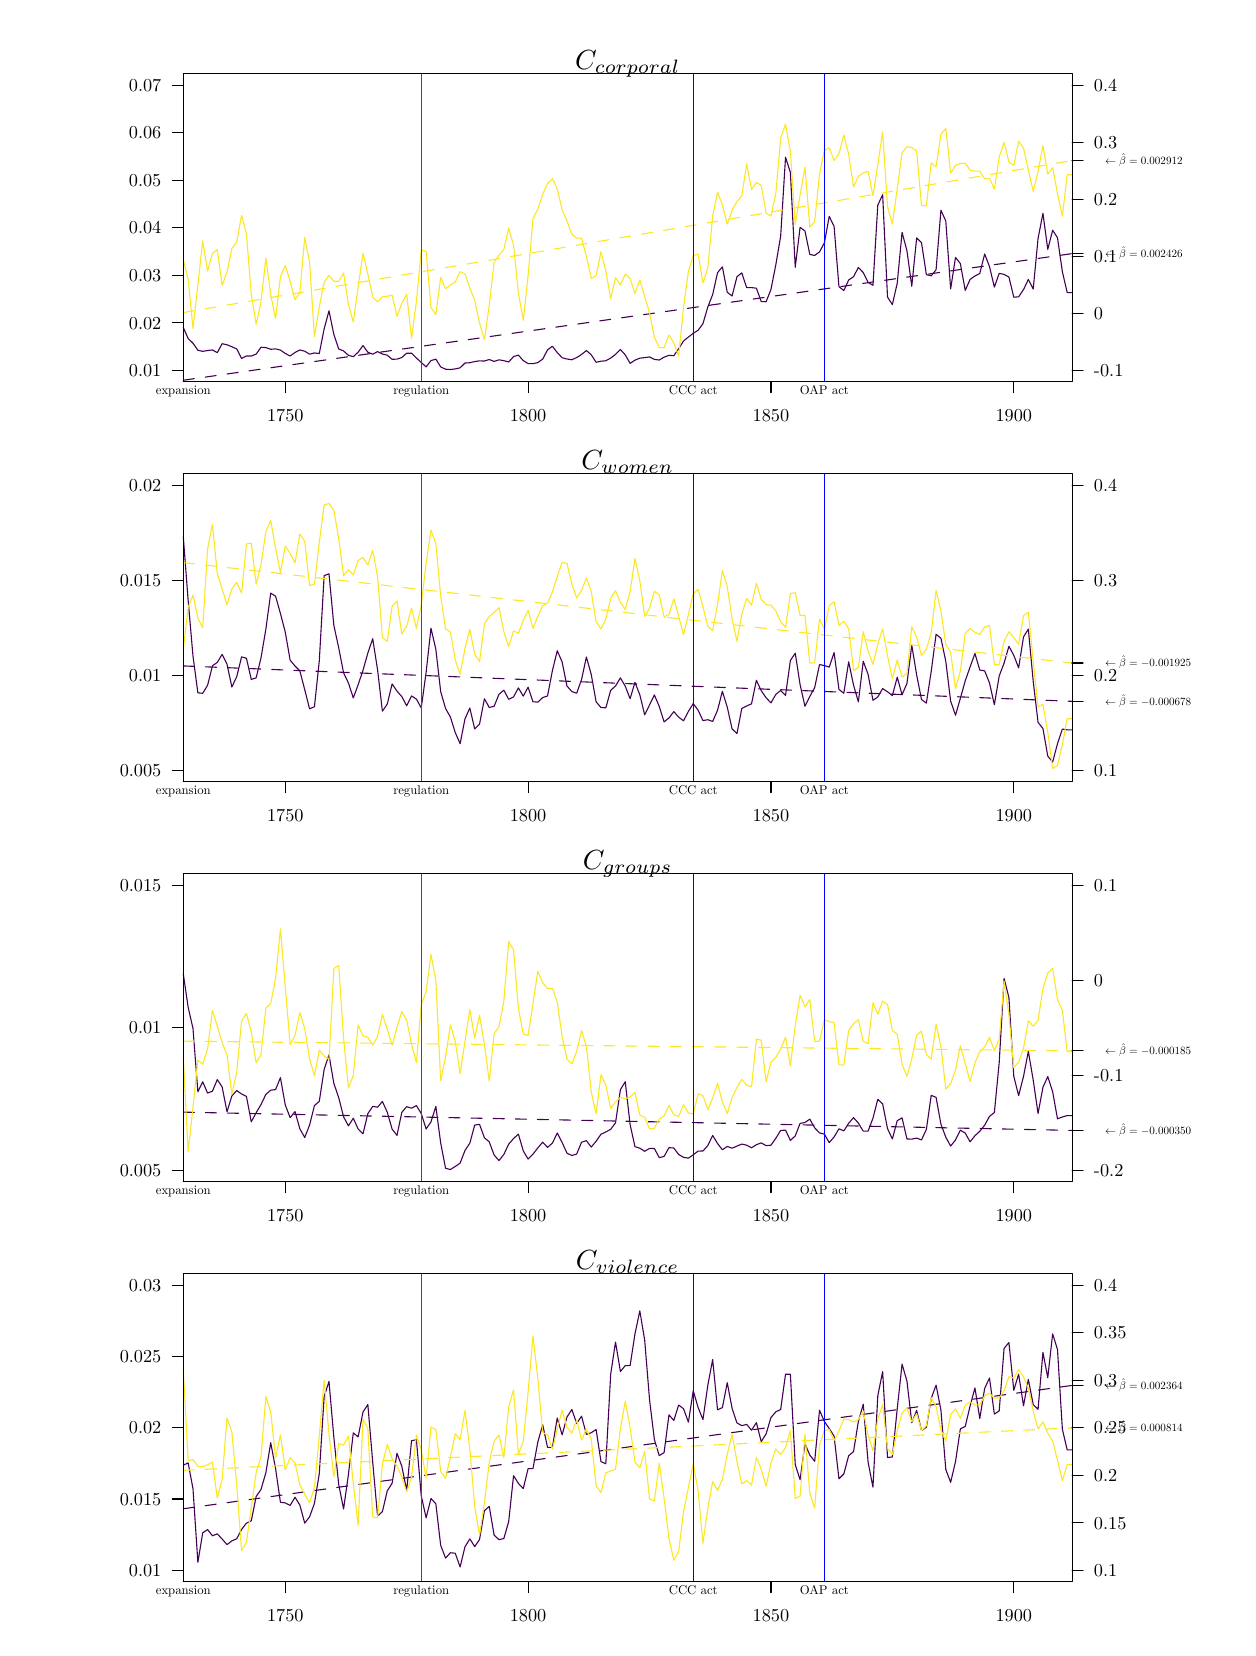
\begin{tikzpicture}[x=1pt,y=1pt]
\definecolor{fillColor}{RGB}{255,255,255}
\path[use as bounding box,fill=fillColor,fill opacity=0.00] (0,0) rectangle (433.62,578.16);
\begin{scope}
\path[clip] (  0.00,  0.00) rectangle (433.62,578.16);
\definecolor{drawColor}{RGB}{0,0,0}

\path[draw=drawColor,line width= 0.4pt,line join=round,line cap=round] ( 93.09,450.25) -- (356.33,450.25);

\path[draw=drawColor,line width= 0.4pt,line join=round,line cap=round] ( 93.09,450.25) -- ( 93.09,446.29);

\path[draw=drawColor,line width= 0.4pt,line join=round,line cap=round] (180.83,450.25) -- (180.83,446.29);

\path[draw=drawColor,line width= 0.4pt,line join=round,line cap=round] (268.58,450.25) -- (268.58,446.29);

\path[draw=drawColor,line width= 0.4pt,line join=round,line cap=round] (356.33,450.25) -- (356.33,446.29);

\node[text=drawColor,anchor=base,inner sep=0pt, outer sep=0pt, scale=  0.66] at ( 93.09,436.00) {1750};

\node[text=drawColor,anchor=base,inner sep=0pt, outer sep=0pt, scale=  0.66] at (180.83,436.00) {1800};

\node[text=drawColor,anchor=base,inner sep=0pt, outer sep=0pt, scale=  0.66] at (268.58,436.00) {1850};

\node[text=drawColor,anchor=base,inner sep=0pt, outer sep=0pt, scale=  0.66] at (356.33,436.00) {1900};
\definecolor{drawColor}{RGB}{68,1,84}

\path[draw=drawColor,line width= 0.4pt,line join=round,line cap=round] ( 56.23,469.80) --
	( 57.99,465.82) --
	( 59.74,464.13) --
	( 61.50,461.59) --
	( 63.25,461.19) --
	( 65.01,461.49) --
	( 66.76,461.70) --
	( 68.52,460.74) --
	( 70.27,463.96) --
	( 72.03,463.57) --
	( 73.78,462.86) --
	( 75.54,462.06) --
	( 77.29,458.63) --
	( 79.05,459.54) --
	( 80.80,459.49) --
	( 82.56,460.19) --
	( 84.31,462.67) --
	( 86.07,462.57) --
	( 87.82,461.93) --
	( 89.58,462.09) --
	( 91.33,461.66) --
	( 93.09,460.43) --
	( 94.84,459.51) --
	( 96.60,460.78) --
	( 98.35,461.70) --
	(100.11,461.25) --
	(101.86,460.16) --
	(103.62,460.62) --
	(105.37,460.40) --
	(107.13,469.32) --
	(108.88,475.83) --
	(110.64,467.25) --
	(112.39,462.07) --
	(114.15,461.34) --
	(115.90,459.76) --
	(117.66,459.26) --
	(119.41,460.89) --
	(121.17,463.30) --
	(122.92,460.88) --
	(124.68,460.15) --
	(126.43,461.12) --
	(128.18,460.24) --
	(129.94,459.80) --
	(131.69,458.32) --
	(133.45,458.39) --
	(135.20,458.98) --
	(136.96,460.52) --
	(138.71,460.52) --
	(140.47,458.79) --
	(142.22,457.16) --
	(143.98,455.58) --
	(145.73,457.85) --
	(147.49,458.38) --
	(149.24,455.57) --
	(151.00,454.74) --
	(152.75,454.62) --
	(154.51,454.85) --
	(156.26,455.24) --
	(158.02,456.97) --
	(159.77,457.08) --
	(161.53,457.50) --
	(163.28,457.76) --
	(165.04,457.69) --
	(166.79,458.24) --
	(168.55,457.55) --
	(170.30,458.13) --
	(172.06,457.83) --
	(173.81,457.35) --
	(175.57,459.29) --
	(177.32,459.83) --
	(179.08,457.86) --
	(180.83,456.76) --
	(182.59,456.75) --
	(184.34,457.12) --
	(186.10,458.39) --
	(187.85,461.73) --
	(189.61,463.05) --
	(191.36,460.75) --
	(193.12,458.89) --
	(194.87,458.42) --
	(196.63,458.16) --
	(198.38,458.94) --
	(200.14,460.07) --
	(201.89,461.49) --
	(203.65,459.95) --
	(205.40,457.24) --
	(207.16,457.63) --
	(208.91,457.79) --
	(210.67,458.77) --
	(212.42,460.11) --
	(214.18,461.85) --
	(215.93,459.94) --
	(217.69,456.86) --
	(219.44,458.02) --
	(221.20,458.73) --
	(222.95,458.93) --
	(224.71,459.18) --
	(226.46,458.29) --
	(228.22,458.06) --
	(229.97,459.09) --
	(231.73,459.76) --
	(233.48,459.62) --
	(235.24,462.17) --
	(236.99,464.93) --
	(238.75,466.36) --
	(240.50,467.71) --
	(242.26,468.80) --
	(244.01,471.20) --
	(245.77,477.26) --
	(247.52,481.72) --
	(249.28,489.62) --
	(251.03,491.74) --
	(252.79,482.53) --
	(254.54,481.20) --
	(256.30,488.17) --
	(258.05,489.53) --
	(259.81,484.24) --
	(261.56,484.23) --
	(263.32,484.01) --
	(265.07,479.19) --
	(266.83,479.12) --
	(268.58,483.54) --
	(270.34,492.49) --
	(272.09,502.80) --
	(273.85,531.35) --
	(275.60,525.84) --
	(277.36,491.55) --
	(279.11,506.00) --
	(280.87,504.69) --
	(282.62,496.21) --
	(284.38,495.85) --
	(286.13,497.13) --
	(287.89,500.41) --
	(289.64,509.97) --
	(291.40,506.32) --
	(293.15,484.55) --
	(294.91,483.17) --
	(296.66,486.96) --
	(298.42,488.16) --
	(300.17,491.51) --
	(301.93,489.67) --
	(303.68,486.10) --
	(305.44,485.07) --
	(307.19,514.04) --
	(308.94,517.80) --
	(310.70,480.80) --
	(312.45,478.10) --
	(314.21,485.80) --
	(315.96,504.20) --
	(317.72,497.54) --
	(319.47,484.73) --
	(321.23,502.17) --
	(322.98,500.46) --
	(324.74,488.93) --
	(326.49,488.49) --
	(328.25,490.68) --
	(330.00,512.18) --
	(331.76,508.31) --
	(333.51,483.74) --
	(335.27,495.13) --
	(337.02,492.90) --
	(338.78,483.22) --
	(340.53,487.18) --
	(342.29,488.43) --
	(344.04,489.30) --
	(345.80,496.38) --
	(347.55,491.84) --
	(349.31,484.41) --
	(351.06,489.38) --
	(352.82,489.00) --
	(354.57,488.03) --
	(356.33,480.75) --
	(358.08,480.91) --
	(359.84,483.50) --
	(361.59,487.17) --
	(363.35,483.69) --
	(365.10,502.00) --
	(366.86,511.06) --
	(368.61,498.06) --
	(370.37,504.95) --
	(372.12,502.25) --
	(373.88,489.99) --
	(375.63,482.43) --
	(377.39,482.43);
\definecolor{drawColor}{RGB}{0,0,0}

\path[draw=drawColor,line width= 0.4pt,line join=round,line cap=round] ( 56.23,454.37) -- ( 56.23,557.41);

\path[draw=drawColor,line width= 0.4pt,line join=round,line cap=round] ( 56.23,454.37) -- ( 52.27,454.37);

\path[draw=drawColor,line width= 0.4pt,line join=round,line cap=round] ( 56.23,471.55) -- ( 52.27,471.55);

\path[draw=drawColor,line width= 0.4pt,line join=round,line cap=round] ( 56.23,488.72) -- ( 52.27,488.72);

\path[draw=drawColor,line width= 0.4pt,line join=round,line cap=round] ( 56.23,505.89) -- ( 52.27,505.89);

\path[draw=drawColor,line width= 0.4pt,line join=round,line cap=round] ( 56.23,523.06) -- ( 52.27,523.06);

\path[draw=drawColor,line width= 0.4pt,line join=round,line cap=round] ( 56.23,540.23) -- ( 52.27,540.23);

\path[draw=drawColor,line width= 0.4pt,line join=round,line cap=round] ( 56.23,557.41) -- ( 52.27,557.41);

\node[text=drawColor,anchor=base east,inner sep=0pt, outer sep=0pt, scale=  0.66] at ( 48.31,452.10) {0.01};

\node[text=drawColor,anchor=base east,inner sep=0pt, outer sep=0pt, scale=  0.66] at ( 48.31,469.27) {0.02};

\node[text=drawColor,anchor=base east,inner sep=0pt, outer sep=0pt, scale=  0.66] at ( 48.31,486.44) {0.03};

\node[text=drawColor,anchor=base east,inner sep=0pt, outer sep=0pt, scale=  0.66] at ( 48.31,503.62) {0.04};

\node[text=drawColor,anchor=base east,inner sep=0pt, outer sep=0pt, scale=  0.66] at ( 48.31,520.79) {0.05};

\node[text=drawColor,anchor=base east,inner sep=0pt, outer sep=0pt, scale=  0.66] at ( 48.31,537.96) {0.06};

\node[text=drawColor,anchor=base east,inner sep=0pt, outer sep=0pt, scale=  0.66] at ( 48.31,555.13) {0.07};
\definecolor{drawColor}{RGB}{68,1,84}

\path[draw=drawColor,line width= 0.4pt,dash pattern=on 4pt off 4pt ,line join=round,line cap=round] ( 56.23,450.76) --
	( 57.99,451.01) --
	( 59.74,451.26) --
	( 61.50,451.51) --
	( 63.25,451.76) --
	( 65.01,452.01) --
	( 66.76,452.26) --
	( 68.52,452.51) --
	( 70.27,452.76) --
	( 72.03,453.01) --
	( 73.78,453.26) --
	( 75.54,453.51) --
	( 77.29,453.76) --
	( 79.05,454.01) --
	( 80.80,454.26) --
	( 82.56,454.51) --
	( 84.31,454.76) --
	( 86.07,455.01) --
	( 87.82,455.26) --
	( 89.58,455.51) --
	( 91.33,455.76) --
	( 93.09,456.01) --
	( 94.84,456.26) --
	( 96.60,456.51) --
	( 98.35,456.76) --
	(100.11,457.01) --
	(101.86,457.26) --
	(103.62,457.51) --
	(105.37,457.76) --
	(107.13,458.01) --
	(108.88,458.26) --
	(110.64,458.51) --
	(112.39,458.76) --
	(114.15,459.01) --
	(115.90,459.26) --
	(117.66,459.51) --
	(119.41,459.76) --
	(121.17,460.01) --
	(122.92,460.26) --
	(124.68,460.51) --
	(126.43,460.76) --
	(128.18,461.01) --
	(129.94,461.26) --
	(131.69,461.51) --
	(133.45,461.76) --
	(135.20,462.01) --
	(136.96,462.26) --
	(138.71,462.51) --
	(140.47,462.76) --
	(142.22,463.01) --
	(143.98,463.26) --
	(145.73,463.51) --
	(147.49,463.76) --
	(149.24,464.01) --
	(151.00,464.26) --
	(152.75,464.51) --
	(154.51,464.76) --
	(156.26,465.01) --
	(158.02,465.26) --
	(159.77,465.51) --
	(161.53,465.76) --
	(163.28,466.01) --
	(165.04,466.26) --
	(166.79,466.51) --
	(168.55,466.76) --
	(170.30,467.01) --
	(172.06,467.26) --
	(173.81,467.51) --
	(175.57,467.76) --
	(177.32,468.01) --
	(179.08,468.26) --
	(180.83,468.51) --
	(182.59,468.76) --
	(184.34,469.01) --
	(186.10,469.26) --
	(187.85,469.51) --
	(189.61,469.76) --
	(191.36,470.01) --
	(193.12,470.26) --
	(194.87,470.51) --
	(196.63,470.76) --
	(198.38,471.01) --
	(200.14,471.26) --
	(201.89,471.51) --
	(203.65,471.76) --
	(205.40,472.01) --
	(207.16,472.26) --
	(208.91,472.51) --
	(210.67,472.76) --
	(212.42,473.01) --
	(214.18,473.26) --
	(215.93,473.51) --
	(217.69,473.76) --
	(219.44,474.01) --
	(221.20,474.26) --
	(222.95,474.51) --
	(224.71,474.76) --
	(226.46,475.01) --
	(228.22,475.26) --
	(229.97,475.51) --
	(231.73,475.76) --
	(233.48,476.01) --
	(235.24,476.26) --
	(236.99,476.51) --
	(238.75,476.76) --
	(240.50,477.01) --
	(242.26,477.26) --
	(244.01,477.51) --
	(245.77,477.76) --
	(247.52,478.01) --
	(249.28,478.26) --
	(251.03,478.51) --
	(252.79,478.76) --
	(254.54,479.01) --
	(256.30,479.26) --
	(258.05,479.51) --
	(259.81,479.76) --
	(261.56,480.01) --
	(263.32,480.26) --
	(265.07,480.51) --
	(266.83,480.76) --
	(268.58,481.01) --
	(270.34,481.26) --
	(272.09,481.51) --
	(273.85,481.76) --
	(275.60,482.01) --
	(277.36,482.26) --
	(279.11,482.51) --
	(280.87,482.76) --
	(282.62,483.01) --
	(284.38,483.26) --
	(286.13,483.51) --
	(287.89,483.76) --
	(289.64,484.01) --
	(291.40,484.26) --
	(293.15,484.51) --
	(294.91,484.76) --
	(296.66,485.01) --
	(298.42,485.26) --
	(300.17,485.51) --
	(301.93,485.76) --
	(303.68,486.01) --
	(305.44,486.26) --
	(307.19,486.51) --
	(308.94,486.76) --
	(310.70,487.01) --
	(312.45,487.26) --
	(314.21,487.51) --
	(315.96,487.76) --
	(317.72,488.01) --
	(319.47,488.26) --
	(321.23,488.51) --
	(322.98,488.76) --
	(324.74,489.01) --
	(326.49,489.26) --
	(328.25,489.51) --
	(330.00,489.76) --
	(331.76,490.01) --
	(333.51,490.26) --
	(335.27,490.51) --
	(337.02,490.76) --
	(338.78,491.01) --
	(340.53,491.26) --
	(342.29,491.51) --
	(344.04,491.76) --
	(345.80,492.01) --
	(347.55,492.26) --
	(349.31,492.51) --
	(351.06,492.76) --
	(352.82,493.01) --
	(354.57,493.26) --
	(356.33,493.51) --
	(358.08,493.76) --
	(359.84,494.01) --
	(361.59,494.26) --
	(363.35,494.51) --
	(365.10,494.76) --
	(366.86,495.01) --
	(368.61,495.26) --
	(370.37,495.51) --
	(372.12,495.76) --
	(373.88,496.01) --
	(375.63,496.26) --
	(377.39,496.51);
\definecolor{drawColor}{RGB}{0,0,0}

\path[draw=drawColor,line width= 0.4pt,line join=round,line cap=round] (377.39,496.51) -- (377.39,496.51);

\path[draw=drawColor,line width= 0.4pt,line join=round,line cap=round] (377.39,496.51) -- (381.35,496.51);

\node[text=drawColor,anchor=base west,inner sep=0pt, outer sep=0pt, scale=  0.40] at (385.31,495.15) {$\quad\leftarrow\hat{\beta}=0.002426$};
\definecolor{drawColor}{RGB}{253,231,37}

\path[draw=drawColor,line width= 0.4pt,line join=round,line cap=round] ( 56.23,494.26) --
	( 57.99,487.27) --
	( 59.74,469.44) --
	( 61.50,485.23) --
	( 63.25,501.03) --
	( 65.01,490.23) --
	( 66.76,496.59) --
	( 68.52,497.93) --
	( 70.27,484.99) --
	( 72.03,489.84) --
	( 73.78,498.38) --
	( 75.54,500.73) --
	( 77.29,510.34) --
	( 79.05,503.63) --
	( 80.80,481.79) --
	( 82.56,470.97) --
	( 84.31,479.08) --
	( 86.07,494.92) --
	( 87.82,481.72) --
	( 89.58,473.01) --
	( 91.33,488.14) --
	( 93.09,492.25) --
	( 94.84,486.47) --
	( 96.60,479.88) --
	( 98.35,482.34) --
	(100.11,502.41) --
	(101.86,493.38) --
	(103.62,466.50) --
	(105.37,477.23) --
	(107.13,486.17) --
	(108.88,488.63) --
	(110.64,486.55) --
	(112.39,486.46) --
	(114.15,489.52) --
	(115.90,478.16) --
	(117.66,471.74) --
	(119.41,484.42) --
	(121.17,496.67) --
	(122.92,489.08) --
	(124.68,480.82) --
	(126.43,479.07) --
	(128.18,480.93) --
	(129.94,481.11) --
	(131.69,481.47) --
	(133.45,473.86) --
	(135.20,478.54) --
	(136.96,481.84) --
	(138.71,465.81) --
	(140.47,479.29) --
	(142.22,497.77) --
	(143.98,497.33) --
	(145.73,477.00) --
	(147.49,474.43) --
	(149.24,487.96) --
	(151.00,483.88) --
	(152.75,485.09) --
	(154.51,486.29) --
	(156.26,489.98) --
	(158.02,489.16) --
	(159.77,484.03) --
	(161.53,479.68) --
	(163.28,471.45) --
	(165.04,465.41) --
	(166.79,477.95) --
	(168.55,493.34) --
	(170.30,495.96) --
	(172.06,497.98) --
	(173.81,505.74) --
	(175.57,499.53) --
	(177.32,482.21) --
	(179.08,472.43) --
	(180.83,488.56) --
	(182.59,509.19) --
	(184.34,512.55) --
	(186.10,517.92) --
	(187.85,521.85) --
	(189.61,523.60) --
	(191.36,519.85) --
	(193.12,512.35) --
	(194.87,508.38) --
	(196.63,503.52) --
	(198.38,502.12) --
	(200.14,502.06) --
	(201.89,495.50) --
	(203.65,487.55) --
	(205.40,488.47) --
	(207.16,497.20) --
	(208.91,490.21) --
	(210.67,480.27) --
	(212.42,487.83) --
	(214.18,485.19) --
	(215.93,489.13) --
	(217.69,487.48) --
	(219.44,482.02) --
	(221.20,487.02) --
	(222.95,481.02) --
	(224.71,475.10) --
	(226.46,466.31) --
	(228.22,462.57) --
	(229.97,462.48) --
	(231.73,467.12) --
	(233.48,464.21) --
	(235.24,459.41) --
	(236.99,477.14) --
	(238.75,490.08) --
	(240.50,495.85) --
	(242.26,496.37) --
	(244.01,485.89) --
	(245.77,491.35) --
	(247.52,510.17) --
	(249.28,518.73) --
	(251.03,514.18) --
	(252.79,507.21) --
	(254.54,512.13) --
	(256.30,515.40) --
	(258.05,517.33) --
	(259.81,528.95) --
	(261.56,519.72) --
	(263.32,522.26) --
	(265.07,521.12) --
	(266.83,511.13) --
	(268.58,510.09) --
	(270.34,518.24) --
	(272.09,538.24) --
	(273.85,543.32) --
	(275.60,533.41) --
	(277.36,507.07) --
	(279.11,517.74) --
	(280.87,527.80) --
	(282.62,506.11) --
	(284.38,508.08) --
	(286.13,525.21) --
	(287.89,533.87) --
	(289.64,534.75) --
	(291.40,530.15) --
	(293.15,532.64) --
	(294.91,539.40) --
	(296.66,532.42) --
	(298.42,520.66) --
	(300.17,524.41) --
	(301.93,525.65) --
	(303.68,526.25) --
	(305.44,517.43) --
	(307.19,528.66) --
	(308.94,540.51) --
	(310.70,513.53) --
	(312.45,507.16) --
	(314.21,520.01) --
	(315.96,532.95) --
	(317.72,535.12) --
	(319.47,534.85) --
	(321.23,533.55) --
	(322.98,513.99) --
	(324.74,513.76) --
	(326.49,529.26) --
	(328.25,527.87) --
	(330.00,539.73) --
	(331.76,541.74) --
	(333.51,525.63) --
	(335.27,528.37) --
	(337.02,529.04) --
	(338.78,529.19) --
	(340.53,526.71) --
	(342.29,526.29) --
	(344.04,526.31) --
	(345.80,523.51) --
	(347.55,523.69) --
	(349.31,519.84) --
	(351.06,531.47) --
	(352.82,536.72) --
	(354.57,529.60) --
	(356.33,528.39) --
	(358.08,537.16) --
	(359.84,534.68) --
	(361.59,526.72) --
	(363.35,519.05) --
	(365.10,526.23) --
	(366.86,535.61) --
	(368.61,525.19) --
	(370.37,527.53) --
	(372.12,518.23) --
	(373.88,510.06) --
	(375.63,525.01) --
	(377.39,525.01);
\definecolor{drawColor}{RGB}{0,0,0}

\path[draw=drawColor,line width= 0.4pt,line join=round,line cap=round] (377.39,454.37) -- (377.39,557.41);

\path[draw=drawColor,line width= 0.4pt,line join=round,line cap=round] (377.39,454.37) -- (381.35,454.37);

\path[draw=drawColor,line width= 0.4pt,line join=round,line cap=round] (377.39,474.98) -- (381.35,474.98);

\path[draw=drawColor,line width= 0.4pt,line join=round,line cap=round] (377.39,495.59) -- (381.35,495.59);

\path[draw=drawColor,line width= 0.4pt,line join=round,line cap=round] (377.39,516.19) -- (381.35,516.19);

\path[draw=drawColor,line width= 0.4pt,line join=round,line cap=round] (377.39,536.80) -- (381.35,536.80);

\path[draw=drawColor,line width= 0.4pt,line join=round,line cap=round] (377.39,557.41) -- (381.35,557.41);

\node[text=drawColor,anchor=base west,inner sep=0pt, outer sep=0pt, scale=  0.66] at (385.31,452.10) {-0.1};

\node[text=drawColor,anchor=base west,inner sep=0pt, outer sep=0pt, scale=  0.66] at (385.31,472.71) {0};

\node[text=drawColor,anchor=base west,inner sep=0pt, outer sep=0pt, scale=  0.66] at (385.31,493.31) {0.1};

\node[text=drawColor,anchor=base west,inner sep=0pt, outer sep=0pt, scale=  0.66] at (385.31,513.92) {0.2};

\node[text=drawColor,anchor=base west,inner sep=0pt, outer sep=0pt, scale=  0.66] at (385.31,534.53) {0.3};

\node[text=drawColor,anchor=base west,inner sep=0pt, outer sep=0pt, scale=  0.66] at (385.31,555.13) {0.4};
\definecolor{drawColor}{RGB}{253,231,37}

\path[draw=drawColor,line width= 0.4pt,dash pattern=on 4pt off 4pt ,line join=round,line cap=round] ( 56.23,475.22) --
	( 57.99,475.52) --
	( 59.74,475.82) --
	( 61.50,476.12) --
	( 63.25,476.42) --
	( 65.01,476.72) --
	( 66.76,477.02) --
	( 68.52,477.32) --
	( 70.27,477.62) --
	( 72.03,477.92) --
	( 73.78,478.22) --
	( 75.54,478.52) --
	( 77.29,478.82) --
	( 79.05,479.13) --
	( 80.80,479.43) --
	( 82.56,479.73) --
	( 84.31,480.03) --
	( 86.07,480.33) --
	( 87.82,480.63) --
	( 89.58,480.93) --
	( 91.33,481.23) --
	( 93.09,481.53) --
	( 94.84,481.83) --
	( 96.60,482.13) --
	( 98.35,482.43) --
	(100.11,482.73) --
	(101.86,483.03) --
	(103.62,483.33) --
	(105.37,483.63) --
	(107.13,483.93) --
	(108.88,484.23) --
	(110.64,484.53) --
	(112.39,484.83) --
	(114.15,485.13) --
	(115.90,485.43) --
	(117.66,485.73) --
	(119.41,486.03) --
	(121.17,486.33) --
	(122.92,486.63) --
	(124.68,486.93) --
	(126.43,487.23) --
	(128.18,487.53) --
	(129.94,487.83) --
	(131.69,488.13) --
	(133.45,488.43) --
	(135.20,488.73) --
	(136.96,489.03) --
	(138.71,489.33) --
	(140.47,489.63) --
	(142.22,489.93) --
	(143.98,490.23) --
	(145.73,490.53) --
	(147.49,490.83) --
	(149.24,491.13) --
	(151.00,491.43) --
	(152.75,491.73) --
	(154.51,492.03) --
	(156.26,492.33) --
	(158.02,492.63) --
	(159.77,492.93) --
	(161.53,493.23) --
	(163.28,493.53) --
	(165.04,493.83) --
	(166.79,494.13) --
	(168.55,494.43) --
	(170.30,494.73) --
	(172.06,495.03) --
	(173.81,495.33) --
	(175.57,495.63) --
	(177.32,495.93) --
	(179.08,496.23) --
	(180.83,496.53) --
	(182.59,496.83) --
	(184.34,497.13) --
	(186.10,497.43) --
	(187.85,497.73) --
	(189.61,498.03) --
	(191.36,498.33) --
	(193.12,498.63) --
	(194.87,498.93) --
	(196.63,499.23) --
	(198.38,499.53) --
	(200.14,499.83) --
	(201.89,500.13) --
	(203.65,500.43) --
	(205.40,500.73) --
	(207.16,501.03) --
	(208.91,501.33) --
	(210.67,501.63) --
	(212.42,501.93) --
	(214.18,502.23) --
	(215.93,502.53) --
	(217.69,502.83) --
	(219.44,503.13) --
	(221.20,503.43) --
	(222.95,503.73) --
	(224.71,504.03) --
	(226.46,504.33) --
	(228.22,504.63) --
	(229.97,504.93) --
	(231.73,505.23) --
	(233.48,505.53) --
	(235.24,505.83) --
	(236.99,506.13) --
	(238.75,506.43) --
	(240.50,506.73) --
	(242.26,507.03) --
	(244.01,507.33) --
	(245.77,507.63) --
	(247.52,507.93) --
	(249.28,508.23) --
	(251.03,508.53) --
	(252.79,508.83) --
	(254.54,509.13) --
	(256.30,509.43) --
	(258.05,509.73) --
	(259.81,510.03) --
	(261.56,510.33) --
	(263.32,510.63) --
	(265.07,510.93) --
	(266.83,511.23) --
	(268.58,511.53) --
	(270.34,511.83) --
	(272.09,512.13) --
	(273.85,512.43) --
	(275.60,512.73) --
	(277.36,513.03) --
	(279.11,513.33) --
	(280.87,513.63) --
	(282.62,513.93) --
	(284.38,514.23) --
	(286.13,514.53) --
	(287.89,514.83) --
	(289.64,515.13) --
	(291.40,515.44) --
	(293.15,515.74) --
	(294.91,516.04) --
	(296.66,516.34) --
	(298.42,516.64) --
	(300.17,516.94) --
	(301.93,517.24) --
	(303.68,517.54) --
	(305.44,517.84) --
	(307.19,518.14) --
	(308.94,518.44) --
	(310.70,518.74) --
	(312.45,519.04) --
	(314.21,519.34) --
	(315.96,519.64) --
	(317.72,519.94) --
	(319.47,520.24) --
	(321.23,520.54) --
	(322.98,520.84) --
	(324.74,521.14) --
	(326.49,521.44) --
	(328.25,521.74) --
	(330.00,522.04) --
	(331.76,522.34) --
	(333.51,522.64) --
	(335.27,522.94) --
	(337.02,523.24) --
	(338.78,523.54) --
	(340.53,523.84) --
	(342.29,524.14) --
	(344.04,524.44) --
	(345.80,524.74) --
	(347.55,525.04) --
	(349.31,525.34) --
	(351.06,525.64) --
	(352.82,525.94) --
	(354.57,526.24) --
	(356.33,526.54) --
	(358.08,526.84) --
	(359.84,527.14) --
	(361.59,527.44) --
	(363.35,527.74) --
	(365.10,528.04) --
	(366.86,528.34) --
	(368.61,528.64) --
	(370.37,528.94) --
	(372.12,529.24) --
	(373.88,529.54) --
	(375.63,529.84) --
	(377.39,530.14);
\definecolor{drawColor}{RGB}{0,0,0}

\path[draw=drawColor,line width= 0.4pt,line join=round,line cap=round] (377.39,530.14) -- (377.39,530.14);

\path[draw=drawColor,line width= 0.4pt,line join=round,line cap=round] (377.39,530.14) -- (381.35,530.14);

\node[text=drawColor,anchor=base west,inner sep=0pt, outer sep=0pt, scale=  0.40] at (385.31,528.78) {$\quad\leftarrow\hat{\beta}=0.002912$};
\end{scope}
\begin{scope}
\path[clip] ( 56.23,450.25) rectangle (377.39,561.53);
\definecolor{drawColor}{RGB}{255,0,0}

\path[draw=drawColor,line width= 0.4pt,line join=round,line cap=round] ( 56.23,450.25) -- ( 56.23,561.53);

\path[draw=drawColor,line width= 0.4pt,line join=round,line cap=round] (142.22,450.25) -- (142.22,561.53);
\definecolor{drawColor}{RGB}{0,0,255}

\path[draw=drawColor,line width= 0.4pt,line join=round,line cap=round] (240.50,450.25) -- (240.50,561.53);

\path[draw=drawColor,line width= 0.4pt,line join=round,line cap=round] (287.89,450.25) -- (287.89,561.53);
\end{scope}
\begin{scope}
\path[clip] (  0.00,  0.00) rectangle (433.62,578.16);
\definecolor{drawColor}{RGB}{0,0,0}

\node[text=drawColor,anchor=base,inner sep=0pt, outer sep=0pt, scale=  0.46] at ( 56.23,445.50) {expansion};

\node[text=drawColor,anchor=base,inner sep=0pt, outer sep=0pt, scale=  0.46] at (142.22,445.50) {regulation};

\node[text=drawColor,anchor=base,inner sep=0pt, outer sep=0pt, scale=  0.46] at (240.50,445.50) {CCC act};

\node[text=drawColor,anchor=base,inner sep=0pt, outer sep=0pt, scale=  0.46] at (287.89,445.50) {OAP act};

\path[draw=drawColor,line width= 0.4pt,line join=round,line cap=round] ( 56.23,450.25) --
	(377.39,450.25) --
	(377.39,561.53) --
	( 56.23,561.53) --
	( 56.23,450.25);

\node[text=drawColor,anchor=base,inner sep=0pt, outer sep=0pt, scale=  1.00] at (216.81,563.11) {$C_{corporal}$};
\end{scope}
\begin{scope}
\path[clip] (  0.00,  0.00) rectangle (433.62,578.16);
\definecolor{drawColor}{RGB}{0,0,0}

\path[draw=drawColor,line width= 0.4pt,line join=round,line cap=round] ( 93.09,305.71) -- (356.33,305.71);

\path[draw=drawColor,line width= 0.4pt,line join=round,line cap=round] ( 93.09,305.71) -- ( 93.09,301.75);

\path[draw=drawColor,line width= 0.4pt,line join=round,line cap=round] (180.83,305.71) -- (180.83,301.75);

\path[draw=drawColor,line width= 0.4pt,line join=round,line cap=round] (268.58,305.71) -- (268.58,301.75);

\path[draw=drawColor,line width= 0.4pt,line join=round,line cap=round] (356.33,305.71) -- (356.33,301.75);

\node[text=drawColor,anchor=base,inner sep=0pt, outer sep=0pt, scale=  0.66] at ( 93.09,291.46) {1750};

\node[text=drawColor,anchor=base,inner sep=0pt, outer sep=0pt, scale=  0.66] at (180.83,291.46) {1800};

\node[text=drawColor,anchor=base,inner sep=0pt, outer sep=0pt, scale=  0.66] at (268.58,291.46) {1850};

\node[text=drawColor,anchor=base,inner sep=0pt, outer sep=0pt, scale=  0.66] at (356.33,291.46) {1900};
\definecolor{drawColor}{RGB}{68,1,84}

\path[draw=drawColor,line width= 0.4pt,line join=round,line cap=round] ( 56.23,394.20) --
	( 57.99,371.15) --
	( 59.74,351.05) --
	( 61.50,337.79) --
	( 63.25,337.63) --
	( 65.01,340.54) --
	( 66.76,347.56) --
	( 68.52,348.79) --
	( 70.27,351.71) --
	( 72.03,348.13) --
	( 73.78,339.91) --
	( 75.54,343.62) --
	( 77.29,350.79) --
	( 79.05,350.29) --
	( 80.80,342.63) --
	( 82.56,343.22) --
	( 84.31,350.45) --
	( 86.07,360.80) --
	( 87.82,373.83) --
	( 89.58,372.72) --
	( 91.33,366.48) --
	( 93.09,359.69) --
	( 94.84,349.60) --
	( 96.60,347.49) --
	( 98.35,345.74) --
	(100.11,338.95) --
	(101.86,332.02) --
	(103.62,332.79) --
	(105.37,349.29) --
	(107.13,380.15) --
	(108.88,380.82) --
	(110.64,362.15) --
	(112.39,354.06) --
	(114.15,345.02) --
	(115.90,341.39) --
	(117.66,335.96) --
	(119.41,340.71) --
	(121.17,345.94) --
	(122.92,352.18) --
	(124.68,357.37) --
	(126.43,346.14) --
	(128.18,331.16) --
	(129.94,333.74) --
	(131.69,341.02) --
	(133.45,338.43) --
	(135.20,336.43) --
	(136.96,333.11) --
	(138.71,336.68) --
	(140.47,335.53) --
	(142.22,332.36) --
	(143.98,345.21) --
	(145.73,361.16) --
	(147.49,353.54) --
	(149.24,338.24) --
	(151.00,332.15) --
	(152.75,329.07) --
	(154.51,323.43) --
	(156.26,319.41) --
	(158.02,328.40) --
	(159.77,332.31) --
	(161.53,324.76) --
	(163.28,326.52) --
	(165.04,335.66) --
	(166.79,332.51) --
	(168.55,332.95) --
	(170.30,337.26) --
	(172.06,338.75) --
	(173.81,335.46) --
	(175.57,336.31) --
	(177.32,339.59) --
	(179.08,336.60) --
	(180.83,339.84) --
	(182.59,334.58) --
	(184.34,334.43) --
	(186.10,336.08) --
	(187.85,336.68) --
	(189.61,345.81) --
	(191.36,353.01) --
	(193.12,348.97) --
	(194.87,340.26) --
	(196.63,338.27) --
	(198.38,337.66) --
	(200.14,342.59) --
	(201.89,350.75) --
	(203.65,344.43) --
	(205.40,334.56) --
	(207.16,332.49) --
	(208.91,332.38) --
	(210.67,338.71) --
	(212.42,340.28) --
	(214.18,343.22) --
	(215.93,340.20) --
	(217.69,335.68) --
	(219.44,341.59) --
	(221.20,337.08) --
	(222.95,329.86) --
	(224.71,333.44) --
	(226.46,337.04) --
	(228.22,332.86) --
	(229.97,327.30) --
	(231.73,328.73) --
	(233.48,331.01) --
	(235.24,329.00) --
	(236.99,327.70) --
	(238.75,331.07) --
	(240.50,333.92) --
	(242.26,331.52) --
	(244.01,327.79) --
	(245.77,328.08) --
	(247.52,327.45) --
	(249.28,331.52) --
	(251.03,338.36) --
	(252.79,332.65) --
	(254.54,324.76) --
	(256.30,323.09) --
	(258.05,332.17) --
	(259.81,333.07) --
	(261.56,333.82) --
	(263.32,342.34) --
	(265.07,338.55) --
	(266.83,336.03) --
	(268.58,334.17) --
	(270.34,337.24) --
	(272.09,338.65) --
	(273.85,336.88) --
	(275.60,349.49) --
	(277.36,352.12) --
	(279.11,340.76) --
	(280.87,332.93) --
	(282.62,336.48) --
	(284.38,339.70) --
	(286.13,348.01) --
	(287.89,347.65) --
	(289.64,347.10) --
	(291.40,352.37) --
	(293.15,339.04) --
	(294.91,337.65) --
	(296.66,349.03) --
	(298.42,340.60) --
	(300.17,334.53) --
	(301.93,349.20) --
	(303.68,344.49) --
	(305.44,335.11) --
	(307.19,336.32) --
	(308.94,339.34) --
	(310.70,338.19) --
	(312.45,336.80) --
	(314.21,343.44) --
	(315.96,337.12) --
	(317.72,341.17) --
	(319.47,354.98) --
	(321.23,344.26) --
	(322.98,335.39) --
	(324.74,334.10) --
	(326.49,345.54) --
	(328.25,358.96) --
	(330.00,357.52) --
	(331.76,349.18) --
	(333.51,334.83) --
	(335.27,329.71) --
	(337.02,335.80) --
	(338.78,342.11) --
	(340.53,347.13) --
	(342.29,352.02) --
	(344.04,346.04) --
	(345.80,345.74) --
	(347.55,341.38) --
	(349.31,333.49) --
	(351.06,343.89) --
	(352.82,348.55) --
	(354.57,354.63) --
	(356.33,351.34) --
	(358.08,346.81) --
	(359.84,358.00) --
	(361.59,360.84) --
	(363.35,341.90) --
	(365.10,327.13) --
	(366.86,324.91) --
	(368.61,314.95) --
	(370.37,312.78) --
	(372.12,319.43) --
	(373.88,324.70) --
	(375.63,324.44) --
	(377.39,324.44);
\definecolor{drawColor}{RGB}{0,0,0}

\path[draw=drawColor,line width= 0.4pt,line join=round,line cap=round] ( 56.23,309.83) -- ( 56.23,412.87);

\path[draw=drawColor,line width= 0.4pt,line join=round,line cap=round] ( 56.23,309.83) -- ( 52.27,309.83);

\path[draw=drawColor,line width= 0.4pt,line join=round,line cap=round] ( 56.23,344.18) -- ( 52.27,344.18);

\path[draw=drawColor,line width= 0.4pt,line join=round,line cap=round] ( 56.23,378.52) -- ( 52.27,378.52);

\path[draw=drawColor,line width= 0.4pt,line join=round,line cap=round] ( 56.23,412.87) -- ( 52.27,412.87);

\node[text=drawColor,anchor=base east,inner sep=0pt, outer sep=0pt, scale=  0.66] at ( 48.31,307.56) {0.005};

\node[text=drawColor,anchor=base east,inner sep=0pt, outer sep=0pt, scale=  0.66] at ( 48.31,341.90) {0.01};

\node[text=drawColor,anchor=base east,inner sep=0pt, outer sep=0pt, scale=  0.66] at ( 48.31,376.25) {0.015};

\node[text=drawColor,anchor=base east,inner sep=0pt, outer sep=0pt, scale=  0.66] at ( 48.31,410.59) {0.02};
\definecolor{drawColor}{RGB}{68,1,84}

\path[draw=drawColor,line width= 0.4pt,dash pattern=on 4pt off 4pt ,line join=round,line cap=round] ( 56.23,347.52) --
	( 57.99,347.45) --
	( 59.74,347.38) --
	( 61.50,347.31) --
	( 63.25,347.24) --
	( 65.01,347.17) --
	( 66.76,347.10) --
	( 68.52,347.03) --
	( 70.27,346.96) --
	( 72.03,346.89) --
	( 73.78,346.82) --
	( 75.54,346.75) --
	( 77.29,346.68) --
	( 79.05,346.61) --
	( 80.80,346.54) --
	( 82.56,346.47) --
	( 84.31,346.40) --
	( 86.07,346.33) --
	( 87.82,346.26) --
	( 89.58,346.19) --
	( 91.33,346.12) --
	( 93.09,346.05) --
	( 94.84,345.98) --
	( 96.60,345.91) --
	( 98.35,345.84) --
	(100.11,345.77) --
	(101.86,345.70) --
	(103.62,345.63) --
	(105.37,345.56) --
	(107.13,345.49) --
	(108.88,345.42) --
	(110.64,345.35) --
	(112.39,345.28) --
	(114.15,345.21) --
	(115.90,345.14) --
	(117.66,345.07) --
	(119.41,345.00) --
	(121.17,344.93) --
	(122.92,344.86) --
	(124.68,344.79) --
	(126.43,344.72) --
	(128.18,344.65) --
	(129.94,344.58) --
	(131.69,344.51) --
	(133.45,344.44) --
	(135.20,344.38) --
	(136.96,344.31) --
	(138.71,344.24) --
	(140.47,344.17) --
	(142.22,344.10) --
	(143.98,344.03) --
	(145.73,343.96) --
	(147.49,343.89) --
	(149.24,343.82) --
	(151.00,343.75) --
	(152.75,343.68) --
	(154.51,343.61) --
	(156.26,343.54) --
	(158.02,343.47) --
	(159.77,343.40) --
	(161.53,343.33) --
	(163.28,343.26) --
	(165.04,343.19) --
	(166.79,343.12) --
	(168.55,343.05) --
	(170.30,342.98) --
	(172.06,342.91) --
	(173.81,342.84) --
	(175.57,342.77) --
	(177.32,342.70) --
	(179.08,342.63) --
	(180.83,342.56) --
	(182.59,342.49) --
	(184.34,342.42) --
	(186.10,342.35) --
	(187.85,342.28) --
	(189.61,342.21) --
	(191.36,342.14) --
	(193.12,342.07) --
	(194.87,342.00) --
	(196.63,341.93) --
	(198.38,341.86) --
	(200.14,341.79) --
	(201.89,341.72) --
	(203.65,341.65) --
	(205.40,341.58) --
	(207.16,341.51) --
	(208.91,341.44) --
	(210.67,341.37) --
	(212.42,341.30) --
	(214.18,341.23) --
	(215.93,341.16) --
	(217.69,341.09) --
	(219.44,341.02) --
	(221.20,340.95) --
	(222.95,340.88) --
	(224.71,340.81) --
	(226.46,340.74) --
	(228.22,340.67) --
	(229.97,340.60) --
	(231.73,340.53) --
	(233.48,340.46) --
	(235.24,340.39) --
	(236.99,340.32) --
	(238.75,340.25) --
	(240.50,340.18) --
	(242.26,340.11) --
	(244.01,340.04) --
	(245.77,339.97) --
	(247.52,339.90) --
	(249.28,339.83) --
	(251.03,339.76) --
	(252.79,339.69) --
	(254.54,339.62) --
	(256.30,339.55) --
	(258.05,339.48) --
	(259.81,339.41) --
	(261.56,339.34) --
	(263.32,339.27) --
	(265.07,339.20) --
	(266.83,339.13) --
	(268.58,339.06) --
	(270.34,338.99) --
	(272.09,338.92) --
	(273.85,338.85) --
	(275.60,338.78) --
	(277.36,338.71) --
	(279.11,338.64) --
	(280.87,338.57) --
	(282.62,338.50) --
	(284.38,338.43) --
	(286.13,338.36) --
	(287.89,338.29) --
	(289.64,338.22) --
	(291.40,338.15) --
	(293.15,338.08) --
	(294.91,338.01) --
	(296.66,337.94) --
	(298.42,337.87) --
	(300.17,337.80) --
	(301.93,337.73) --
	(303.68,337.66) --
	(305.44,337.59) --
	(307.19,337.53) --
	(308.94,337.46) --
	(310.70,337.39) --
	(312.45,337.32) --
	(314.21,337.25) --
	(315.96,337.18) --
	(317.72,337.11) --
	(319.47,337.04) --
	(321.23,336.97) --
	(322.98,336.90) --
	(324.74,336.83) --
	(326.49,336.76) --
	(328.25,336.69) --
	(330.00,336.62) --
	(331.76,336.55) --
	(333.51,336.48) --
	(335.27,336.41) --
	(337.02,336.34) --
	(338.78,336.27) --
	(340.53,336.20) --
	(342.29,336.13) --
	(344.04,336.06) --
	(345.80,335.99) --
	(347.55,335.92) --
	(349.31,335.85) --
	(351.06,335.78) --
	(352.82,335.71) --
	(354.57,335.64) --
	(356.33,335.57) --
	(358.08,335.50) --
	(359.84,335.43) --
	(361.59,335.36) --
	(363.35,335.29) --
	(365.10,335.22) --
	(366.86,335.15) --
	(368.61,335.08) --
	(370.37,335.01) --
	(372.12,334.94) --
	(373.88,334.87) --
	(375.63,334.80) --
	(377.39,334.73);
\definecolor{drawColor}{RGB}{0,0,0}

\path[draw=drawColor,line width= 0.4pt,line join=round,line cap=round] (377.39,334.73) -- (377.39,334.73);

\path[draw=drawColor,line width= 0.4pt,line join=round,line cap=round] (377.39,334.73) -- (381.35,334.73);

\node[text=drawColor,anchor=base west,inner sep=0pt, outer sep=0pt, scale=  0.40] at (385.31,333.37) {$\quad\leftarrow\hat{\beta}=-0.000678$};
\definecolor{drawColor}{RGB}{253,231,37}

\path[draw=drawColor,line width= 0.4pt,line join=round,line cap=round] ( 56.23,353.60) --
	( 57.99,368.67) --
	( 59.74,373.16) --
	( 61.50,364.78) --
	( 63.25,361.36) --
	( 65.01,389.78) --
	( 66.76,398.73) --
	( 68.52,380.81) --
	( 70.27,375.40) --
	( 72.03,369.57) --
	( 73.78,375.33) --
	( 75.54,377.70) --
	( 77.29,373.83) --
	( 79.05,391.57) --
	( 80.80,391.92) --
	( 82.56,377.04) --
	( 84.31,384.10) --
	( 86.07,396.09) --
	( 87.82,400.01) --
	( 89.58,390.12) --
	( 91.33,381.23) --
	( 93.09,390.86) --
	( 94.84,388.20) --
	( 96.60,384.76) --
	( 98.35,395.22) --
	(100.11,392.53) --
	(101.86,376.59) --
	(103.62,376.97) --
	(105.37,392.12) --
	(107.13,405.69) --
	(108.88,406.22) --
	(110.64,403.82) --
	(112.39,393.53) --
	(114.15,380.05) --
	(115.90,382.26) --
	(117.66,380.42) --
	(119.41,385.61) --
	(121.17,386.70) --
	(122.92,383.99) --
	(124.68,389.26) --
	(126.43,379.78) --
	(128.18,357.81) --
	(129.94,356.35) --
	(131.69,369.11) --
	(133.45,371.01) --
	(135.20,359.03) --
	(136.96,361.99) --
	(138.71,368.38) --
	(140.47,361.01) --
	(142.22,369.68) --
	(143.98,384.57) --
	(145.73,396.65) --
	(147.49,391.73) --
	(149.24,372.73) --
	(151.00,360.92) --
	(152.75,359.73) --
	(154.51,349.63) --
	(156.26,344.53) --
	(158.02,353.80) --
	(159.77,360.78) --
	(161.53,351.75) --
	(163.28,349.10) --
	(165.04,362.79) --
	(166.79,365.33) --
	(168.55,366.87) --
	(170.30,368.58) --
	(172.06,359.91) --
	(173.81,354.53) --
	(175.57,360.17) --
	(177.32,359.33) --
	(179.08,363.94) --
	(180.83,367.56) --
	(182.59,361.13) --
	(184.34,365.54) --
	(186.10,369.37) --
	(187.85,370.14) --
	(189.61,374.26) --
	(191.36,379.81) --
	(193.12,384.93) --
	(194.87,384.58) --
	(196.63,377.12) --
	(198.38,372.12) --
	(200.14,374.83) --
	(201.89,379.33) --
	(203.65,374.38) --
	(205.40,363.54) --
	(207.16,360.85) --
	(208.91,364.45) --
	(210.67,371.93) --
	(212.42,374.69) --
	(214.18,370.53) --
	(215.93,367.93) --
	(217.69,374.41) --
	(219.44,386.32) --
	(221.20,378.26) --
	(222.95,365.43) --
	(224.71,368.40) --
	(226.46,374.51) --
	(228.22,373.17) --
	(229.97,365.16) --
	(231.73,366.24) --
	(233.48,371.74) --
	(235.24,365.45) --
	(236.99,358.79) --
	(238.75,366.09) --
	(240.50,373.59) --
	(242.26,375.19) --
	(244.01,368.91) --
	(245.77,361.77) --
	(247.52,360.32) --
	(249.28,369.61) --
	(251.03,382.04) --
	(252.79,376.12) --
	(254.54,364.55) --
	(256.30,356.44) --
	(258.05,366.28) --
	(259.81,371.89) --
	(261.56,369.51) --
	(263.32,377.39) --
	(265.07,371.57) --
	(266.83,369.68) --
	(268.58,369.45) --
	(270.34,367.42) --
	(272.09,363.49) --
	(273.85,361.52) --
	(275.60,373.60) --
	(277.36,373.99) --
	(279.11,365.80) --
	(280.87,365.77) --
	(282.62,348.52) --
	(284.38,348.66) --
	(286.13,364.50) --
	(287.89,360.83) --
	(289.64,369.31) --
	(291.40,370.68) --
	(293.15,362.21) --
	(294.91,363.60) --
	(296.66,361.06) --
	(298.42,345.89) --
	(300.17,346.93) --
	(301.93,359.90) --
	(303.68,352.85) --
	(305.44,348.10) --
	(307.19,355.41) --
	(308.94,360.95) --
	(310.70,351.25) --
	(312.45,342.85) --
	(314.21,349.68) --
	(315.96,343.47) --
	(317.72,344.82) --
	(319.47,361.72) --
	(321.23,357.97) --
	(322.98,351.29) --
	(324.74,353.57) --
	(326.49,359.38) --
	(328.25,374.85) --
	(330.00,367.29) --
	(331.76,355.37) --
	(333.51,352.40) --
	(335.27,339.28) --
	(337.02,345.71) --
	(338.78,359.37) --
	(340.53,361.07) --
	(342.29,359.65) --
	(344.04,358.89) --
	(345.80,361.57) --
	(347.55,362.11) --
	(349.31,347.91) --
	(351.06,348.01) --
	(352.82,356.42) --
	(354.57,359.88) --
	(356.33,357.79) --
	(358.08,355.31) --
	(359.84,365.67) --
	(361.59,366.94) --
	(363.35,349.18) --
	(365.10,332.69) --
	(366.86,333.71) --
	(368.61,323.51) --
	(370.37,310.45) --
	(372.12,311.59) --
	(373.88,319.14) --
	(375.63,328.44) --
	(377.39,328.44);
\definecolor{drawColor}{RGB}{0,0,0}

\path[draw=drawColor,line width= 0.4pt,line join=round,line cap=round] (377.39,309.83) -- (377.39,412.87);

\path[draw=drawColor,line width= 0.4pt,line join=round,line cap=round] (377.39,309.83) -- (381.35,309.83);

\path[draw=drawColor,line width= 0.4pt,line join=round,line cap=round] (377.39,344.18) -- (381.35,344.18);

\path[draw=drawColor,line width= 0.4pt,line join=round,line cap=round] (377.39,378.52) -- (381.35,378.52);

\path[draw=drawColor,line width= 0.4pt,line join=round,line cap=round] (377.39,412.87) -- (381.35,412.87);

\node[text=drawColor,anchor=base west,inner sep=0pt, outer sep=0pt, scale=  0.66] at (385.31,307.56) {0.1};

\node[text=drawColor,anchor=base west,inner sep=0pt, outer sep=0pt, scale=  0.66] at (385.31,341.90) {0.2};

\node[text=drawColor,anchor=base west,inner sep=0pt, outer sep=0pt, scale=  0.66] at (385.31,376.25) {0.3};

\node[text=drawColor,anchor=base west,inner sep=0pt, outer sep=0pt, scale=  0.66] at (385.31,410.59) {0.4};
\definecolor{drawColor}{RGB}{253,231,37}

\path[draw=drawColor,line width= 0.4pt,dash pattern=on 4pt off 4pt ,line join=round,line cap=round] ( 56.23,384.86) --
	( 57.99,384.67) --
	( 59.74,384.47) --
	( 61.50,384.27) --
	( 63.25,384.07) --
	( 65.01,383.87) --
	( 66.76,383.67) --
	( 68.52,383.48) --
	( 70.27,383.28) --
	( 72.03,383.08) --
	( 73.78,382.88) --
	( 75.54,382.68) --
	( 77.29,382.48) --
	( 79.05,382.29) --
	( 80.80,382.09) --
	( 82.56,381.89) --
	( 84.31,381.69) --
	( 86.07,381.49) --
	( 87.82,381.29) --
	( 89.58,381.10) --
	( 91.33,380.90) --
	( 93.09,380.70) --
	( 94.84,380.50) --
	( 96.60,380.30) --
	( 98.35,380.10) --
	(100.11,379.91) --
	(101.86,379.71) --
	(103.62,379.51) --
	(105.37,379.31) --
	(107.13,379.11) --
	(108.88,378.91) --
	(110.64,378.72) --
	(112.39,378.52) --
	(114.15,378.32) --
	(115.90,378.12) --
	(117.66,377.92) --
	(119.41,377.72) --
	(121.17,377.53) --
	(122.92,377.33) --
	(124.68,377.13) --
	(126.43,376.93) --
	(128.18,376.73) --
	(129.94,376.53) --
	(131.69,376.34) --
	(133.45,376.14) --
	(135.20,375.94) --
	(136.96,375.74) --
	(138.71,375.54) --
	(140.47,375.34) --
	(142.22,375.15) --
	(143.98,374.95) --
	(145.73,374.75) --
	(147.49,374.55) --
	(149.24,374.35) --
	(151.00,374.15) --
	(152.75,373.96) --
	(154.51,373.76) --
	(156.26,373.56) --
	(158.02,373.36) --
	(159.77,373.16) --
	(161.53,372.96) --
	(163.28,372.77) --
	(165.04,372.57) --
	(166.79,372.37) --
	(168.55,372.17) --
	(170.30,371.97) --
	(172.06,371.77) --
	(173.81,371.58) --
	(175.57,371.38) --
	(177.32,371.18) --
	(179.08,370.98) --
	(180.83,370.78) --
	(182.59,370.58) --
	(184.34,370.39) --
	(186.10,370.19) --
	(187.85,369.99) --
	(189.61,369.79) --
	(191.36,369.59) --
	(193.12,369.39) --
	(194.87,369.20) --
	(196.63,369.00) --
	(198.38,368.80) --
	(200.14,368.60) --
	(201.89,368.40) --
	(203.65,368.20) --
	(205.40,368.01) --
	(207.16,367.81) --
	(208.91,367.61) --
	(210.67,367.41) --
	(212.42,367.21) --
	(214.18,367.01) --
	(215.93,366.82) --
	(217.69,366.62) --
	(219.44,366.42) --
	(221.20,366.22) --
	(222.95,366.02) --
	(224.71,365.82) --
	(226.46,365.63) --
	(228.22,365.43) --
	(229.97,365.23) --
	(231.73,365.03) --
	(233.48,364.83) --
	(235.24,364.63) --
	(236.99,364.44) --
	(238.75,364.24) --
	(240.50,364.04) --
	(242.26,363.84) --
	(244.01,363.64) --
	(245.77,363.44) --
	(247.52,363.25) --
	(249.28,363.05) --
	(251.03,362.85) --
	(252.79,362.65) --
	(254.54,362.45) --
	(256.30,362.25) --
	(258.05,362.06) --
	(259.81,361.86) --
	(261.56,361.66) --
	(263.32,361.46) --
	(265.07,361.26) --
	(266.83,361.06) --
	(268.58,360.87) --
	(270.34,360.67) --
	(272.09,360.47) --
	(273.85,360.27) --
	(275.60,360.07) --
	(277.36,359.87) --
	(279.11,359.68) --
	(280.87,359.48) --
	(282.62,359.28) --
	(284.38,359.08) --
	(286.13,358.88) --
	(287.89,358.68) --
	(289.64,358.49) --
	(291.40,358.29) --
	(293.15,358.09) --
	(294.91,357.89) --
	(296.66,357.69) --
	(298.42,357.49) --
	(300.17,357.30) --
	(301.93,357.10) --
	(303.68,356.90) --
	(305.44,356.70) --
	(307.19,356.50) --
	(308.94,356.30) --
	(310.70,356.11) --
	(312.45,355.91) --
	(314.21,355.71) --
	(315.96,355.51) --
	(317.72,355.31) --
	(319.47,355.11) --
	(321.23,354.92) --
	(322.98,354.72) --
	(324.74,354.52) --
	(326.49,354.32) --
	(328.25,354.12) --
	(330.00,353.92) --
	(331.76,353.73) --
	(333.51,353.53) --
	(335.27,353.33) --
	(337.02,353.13) --
	(338.78,352.93) --
	(340.53,352.73) --
	(342.29,352.54) --
	(344.04,352.34) --
	(345.80,352.14) --
	(347.55,351.94) --
	(349.31,351.74) --
	(351.06,351.54) --
	(352.82,351.35) --
	(354.57,351.15) --
	(356.33,350.95) --
	(358.08,350.75) --
	(359.84,350.55) --
	(361.59,350.35) --
	(363.35,350.16) --
	(365.10,349.96) --
	(366.86,349.76) --
	(368.61,349.56) --
	(370.37,349.36) --
	(372.12,349.16) --
	(373.88,348.97) --
	(375.63,348.77) --
	(377.39,348.57);
\definecolor{drawColor}{RGB}{0,0,0}

\path[draw=drawColor,line width= 0.4pt,line join=round,line cap=round] (377.39,348.57) -- (377.39,348.57);

\path[draw=drawColor,line width= 0.4pt,line join=round,line cap=round] (377.39,348.57) -- (381.35,348.57);

\node[text=drawColor,anchor=base west,inner sep=0pt, outer sep=0pt, scale=  0.40] at (385.31,347.21) {$\quad\leftarrow\hat{\beta}=-0.001925$};
\end{scope}
\begin{scope}
\path[clip] ( 56.23,305.71) rectangle (377.39,416.99);
\definecolor{drawColor}{RGB}{255,0,0}

\path[draw=drawColor,line width= 0.4pt,line join=round,line cap=round] ( 56.23,305.71) -- ( 56.23,416.99);

\path[draw=drawColor,line width= 0.4pt,line join=round,line cap=round] (142.22,305.71) -- (142.22,416.99);
\definecolor{drawColor}{RGB}{0,0,255}

\path[draw=drawColor,line width= 0.4pt,line join=round,line cap=round] (240.50,305.71) -- (240.50,416.99);

\path[draw=drawColor,line width= 0.4pt,line join=round,line cap=round] (287.89,305.71) -- (287.89,416.99);
\end{scope}
\begin{scope}
\path[clip] (  0.00,  0.00) rectangle (433.62,578.16);
\definecolor{drawColor}{RGB}{0,0,0}

\node[text=drawColor,anchor=base,inner sep=0pt, outer sep=0pt, scale=  0.46] at ( 56.23,300.96) {expansion};

\node[text=drawColor,anchor=base,inner sep=0pt, outer sep=0pt, scale=  0.46] at (142.22,300.96) {regulation};

\node[text=drawColor,anchor=base,inner sep=0pt, outer sep=0pt, scale=  0.46] at (240.50,300.96) {CCC act};

\node[text=drawColor,anchor=base,inner sep=0pt, outer sep=0pt, scale=  0.46] at (287.89,300.96) {OAP act};

\path[draw=drawColor,line width= 0.4pt,line join=round,line cap=round] ( 56.23,305.71) --
	(377.39,305.71) --
	(377.39,416.99) --
	( 56.23,416.99) --
	( 56.23,305.71);

\node[text=drawColor,anchor=base,inner sep=0pt, outer sep=0pt, scale=  1.00] at (216.81,418.57) {$C_{women}$};
\end{scope}
\begin{scope}
\path[clip] (  0.00,  0.00) rectangle (433.62,578.16);
\definecolor{drawColor}{RGB}{0,0,0}

\path[draw=drawColor,line width= 0.4pt,line join=round,line cap=round] ( 93.09,161.17) -- (356.33,161.17);

\path[draw=drawColor,line width= 0.4pt,line join=round,line cap=round] ( 93.09,161.17) -- ( 93.09,157.21);

\path[draw=drawColor,line width= 0.4pt,line join=round,line cap=round] (180.83,161.17) -- (180.83,157.21);

\path[draw=drawColor,line width= 0.4pt,line join=round,line cap=round] (268.58,161.17) -- (268.58,157.21);

\path[draw=drawColor,line width= 0.4pt,line join=round,line cap=round] (356.33,161.17) -- (356.33,157.21);

\node[text=drawColor,anchor=base,inner sep=0pt, outer sep=0pt, scale=  0.66] at ( 93.09,146.92) {1750};

\node[text=drawColor,anchor=base,inner sep=0pt, outer sep=0pt, scale=  0.66] at (180.83,146.92) {1800};

\node[text=drawColor,anchor=base,inner sep=0pt, outer sep=0pt, scale=  0.66] at (268.58,146.92) {1850};

\node[text=drawColor,anchor=base,inner sep=0pt, outer sep=0pt, scale=  0.66] at (356.33,146.92) {1900};
\definecolor{drawColor}{RGB}{68,1,84}

\path[draw=drawColor,line width= 0.4pt,line join=round,line cap=round] ( 56.23,236.21) --
	( 57.99,224.17) --
	( 59.74,216.49) --
	( 61.50,193.63) --
	( 63.25,197.25) --
	( 65.01,193.18) --
	( 66.76,193.84) --
	( 68.52,198.05) --
	( 70.27,195.38) --
	( 72.03,186.42) --
	( 73.78,192.13) --
	( 75.54,194.09) --
	( 77.29,192.84) --
	( 79.05,191.95) --
	( 80.80,182.80) --
	( 82.56,186.07) --
	( 84.31,189.02) --
	( 86.07,192.70) --
	( 87.82,194.23) --
	( 89.58,194.42) --
	( 91.33,198.76) --
	( 93.09,188.86) --
	( 94.84,184.29) --
	( 96.60,186.50) --
	( 98.35,180.27) --
	(100.11,177.13) --
	(101.86,181.58) --
	(103.62,188.67) --
	(105.37,190.16) --
	(107.13,201.70) --
	(108.88,206.97) --
	(110.64,196.64) --
	(112.39,191.53) --
	(114.15,184.61) --
	(115.90,181.31) --
	(117.66,184.09) --
	(119.41,180.21) --
	(121.17,178.46) --
	(122.92,185.75) --
	(124.68,188.39) --
	(126.43,188.06) --
	(128.18,190.14) --
	(129.94,186.24) --
	(131.69,180.14) --
	(133.45,177.88) --
	(135.20,186.23) --
	(136.96,188.26) --
	(138.71,187.71) --
	(140.47,188.66) --
	(142.22,185.77) --
	(143.98,180.20) --
	(145.73,182.76) --
	(147.49,188.35) --
	(149.24,175.15) --
	(151.00,166.00) --
	(152.75,165.56) --
	(154.51,166.66) --
	(156.26,167.86) --
	(158.02,172.43) --
	(159.77,175.05) --
	(161.53,181.61) --
	(163.28,181.88) --
	(165.04,177.04) --
	(166.79,175.54) --
	(168.55,170.80) --
	(170.30,168.78) --
	(172.06,171.01) --
	(173.81,174.71) --
	(175.57,176.75) --
	(177.32,178.34) --
	(179.08,172.30) --
	(180.83,169.32) --
	(182.59,171.11) --
	(184.34,173.36) --
	(186.10,175.43) --
	(187.85,173.55) --
	(189.61,175.11) --
	(191.36,178.74) --
	(193.12,175.33) --
	(194.87,171.47) --
	(196.63,170.61) --
	(198.38,171.14) --
	(200.14,175.42) --
	(201.89,175.97) --
	(203.65,173.67) --
	(205.40,175.77) --
	(207.16,178.30) --
	(208.91,179.13) --
	(210.67,180.08) --
	(212.42,182.44) --
	(214.18,194.42) --
	(215.93,197.28) --
	(217.69,181.80) --
	(219.44,173.81) --
	(221.20,173.26) --
	(222.95,172.14) --
	(224.71,173.19) --
	(226.46,173.14) --
	(228.22,169.84) --
	(229.97,170.29) --
	(231.73,173.45) --
	(233.48,173.32) --
	(235.24,170.98) --
	(236.99,169.96) --
	(238.75,169.66) --
	(240.50,170.87) --
	(242.26,172.21) --
	(244.01,172.24) --
	(245.77,174.22) --
	(247.52,177.86) --
	(249.28,174.96) --
	(251.03,172.68) --
	(252.79,173.90) --
	(254.54,173.25) --
	(256.30,174.03) --
	(258.05,174.75) --
	(259.81,174.35) --
	(261.56,173.40) --
	(263.32,174.52) --
	(265.07,175.18) --
	(266.83,174.17) --
	(268.58,174.34) --
	(270.34,176.84) --
	(272.09,179.67) --
	(273.85,179.78) --
	(275.60,176.08) --
	(277.36,177.70) --
	(279.11,182.23) --
	(280.87,182.53) --
	(282.62,183.76) --
	(284.38,180.60) --
	(286.13,178.79) --
	(287.89,178.33) --
	(289.64,175.27) --
	(291.40,177.32) --
	(293.15,180.26) --
	(294.91,179.52) --
	(296.66,182.25) --
	(298.42,184.30) --
	(300.17,182.34) --
	(301.93,179.41) --
	(303.68,179.42) --
	(305.44,184.10) --
	(307.19,190.91) --
	(308.94,189.27) --
	(310.70,180.34) --
	(312.45,176.58) --
	(314.21,183.20) --
	(315.96,184.20) --
	(317.72,176.60) --
	(319.47,176.53) --
	(321.23,176.90) --
	(322.98,176.24) --
	(324.74,180.05) --
	(326.49,192.36) --
	(328.25,191.62) --
	(330.00,181.95) --
	(331.76,177.23) --
	(333.51,174.03) --
	(335.27,176.25) --
	(337.02,179.76) --
	(338.78,178.74) --
	(340.53,175.55) --
	(342.29,177.77) --
	(344.04,179.37) --
	(345.80,181.56) --
	(347.55,184.76) --
	(349.31,186.14) --
	(351.06,204.23) --
	(352.82,234.61) --
	(354.57,227.70) --
	(356.33,199.26) --
	(358.08,192.27) --
	(359.84,199.17) --
	(361.59,208.23) --
	(363.35,197.84) --
	(365.10,185.80) --
	(366.86,195.25) --
	(368.61,199.15) --
	(370.37,193.64) --
	(372.12,183.88) --
	(373.88,184.54) --
	(375.63,185.04) --
	(377.39,185.04);
\definecolor{drawColor}{RGB}{0,0,0}

\path[draw=drawColor,line width= 0.4pt,line join=round,line cap=round] ( 56.23,165.29) -- ( 56.23,268.33);

\path[draw=drawColor,line width= 0.4pt,line join=round,line cap=round] ( 56.23,165.29) -- ( 52.27,165.29);

\path[draw=drawColor,line width= 0.4pt,line join=round,line cap=round] ( 56.23,216.81) -- ( 52.27,216.81);

\path[draw=drawColor,line width= 0.4pt,line join=round,line cap=round] ( 56.23,268.33) -- ( 52.27,268.33);

\node[text=drawColor,anchor=base east,inner sep=0pt, outer sep=0pt, scale=  0.66] at ( 48.31,163.02) {0.005};

\node[text=drawColor,anchor=base east,inner sep=0pt, outer sep=0pt, scale=  0.66] at ( 48.31,214.54) {0.01};

\node[text=drawColor,anchor=base east,inner sep=0pt, outer sep=0pt, scale=  0.66] at ( 48.31,266.05) {0.015};
\definecolor{drawColor}{RGB}{68,1,84}

\path[draw=drawColor,line width= 0.4pt,dash pattern=on 4pt off 4pt ,line join=round,line cap=round] ( 56.23,186.28) --
	( 57.99,186.25) --
	( 59.74,186.21) --
	( 61.50,186.18) --
	( 63.25,186.14) --
	( 65.01,186.10) --
	( 66.76,186.07) --
	( 68.52,186.03) --
	( 70.27,186.00) --
	( 72.03,185.96) --
	( 73.78,185.92) --
	( 75.54,185.89) --
	( 77.29,185.85) --
	( 79.05,185.82) --
	( 80.80,185.78) --
	( 82.56,185.74) --
	( 84.31,185.71) --
	( 86.07,185.67) --
	( 87.82,185.64) --
	( 89.58,185.60) --
	( 91.33,185.56) --
	( 93.09,185.53) --
	( 94.84,185.49) --
	( 96.60,185.46) --
	( 98.35,185.42) --
	(100.11,185.38) --
	(101.86,185.35) --
	(103.62,185.31) --
	(105.37,185.27) --
	(107.13,185.24) --
	(108.88,185.20) --
	(110.64,185.17) --
	(112.39,185.13) --
	(114.15,185.09) --
	(115.90,185.06) --
	(117.66,185.02) --
	(119.41,184.99) --
	(121.17,184.95) --
	(122.92,184.91) --
	(124.68,184.88) --
	(126.43,184.84) --
	(128.18,184.81) --
	(129.94,184.77) --
	(131.69,184.73) --
	(133.45,184.70) --
	(135.20,184.66) --
	(136.96,184.63) --
	(138.71,184.59) --
	(140.47,184.55) --
	(142.22,184.52) --
	(143.98,184.48) --
	(145.73,184.45) --
	(147.49,184.41) --
	(149.24,184.37) --
	(151.00,184.34) --
	(152.75,184.30) --
	(154.51,184.27) --
	(156.26,184.23) --
	(158.02,184.19) --
	(159.77,184.16) --
	(161.53,184.12) --
	(163.28,184.08) --
	(165.04,184.05) --
	(166.79,184.01) --
	(168.55,183.98) --
	(170.30,183.94) --
	(172.06,183.90) --
	(173.81,183.87) --
	(175.57,183.83) --
	(177.32,183.80) --
	(179.08,183.76) --
	(180.83,183.72) --
	(182.59,183.69) --
	(184.34,183.65) --
	(186.10,183.62) --
	(187.85,183.58) --
	(189.61,183.54) --
	(191.36,183.51) --
	(193.12,183.47) --
	(194.87,183.44) --
	(196.63,183.40) --
	(198.38,183.36) --
	(200.14,183.33) --
	(201.89,183.29) --
	(203.65,183.26) --
	(205.40,183.22) --
	(207.16,183.18) --
	(208.91,183.15) --
	(210.67,183.11) --
	(212.42,183.08) --
	(214.18,183.04) --
	(215.93,183.00) --
	(217.69,182.97) --
	(219.44,182.93) --
	(221.20,182.89) --
	(222.95,182.86) --
	(224.71,182.82) --
	(226.46,182.79) --
	(228.22,182.75) --
	(229.97,182.71) --
	(231.73,182.68) --
	(233.48,182.64) --
	(235.24,182.61) --
	(236.99,182.57) --
	(238.75,182.53) --
	(240.50,182.50) --
	(242.26,182.46) --
	(244.01,182.43) --
	(245.77,182.39) --
	(247.52,182.35) --
	(249.28,182.32) --
	(251.03,182.28) --
	(252.79,182.25) --
	(254.54,182.21) --
	(256.30,182.17) --
	(258.05,182.14) --
	(259.81,182.10) --
	(261.56,182.07) --
	(263.32,182.03) --
	(265.07,181.99) --
	(266.83,181.96) --
	(268.58,181.92) --
	(270.34,181.89) --
	(272.09,181.85) --
	(273.85,181.81) --
	(275.60,181.78) --
	(277.36,181.74) --
	(279.11,181.70) --
	(280.87,181.67) --
	(282.62,181.63) --
	(284.38,181.60) --
	(286.13,181.56) --
	(287.89,181.52) --
	(289.64,181.49) --
	(291.40,181.45) --
	(293.15,181.42) --
	(294.91,181.38) --
	(296.66,181.34) --
	(298.42,181.31) --
	(300.17,181.27) --
	(301.93,181.24) --
	(303.68,181.20) --
	(305.44,181.16) --
	(307.19,181.13) --
	(308.94,181.09) --
	(310.70,181.06) --
	(312.45,181.02) --
	(314.21,180.98) --
	(315.96,180.95) --
	(317.72,180.91) --
	(319.47,180.88) --
	(321.23,180.84) --
	(322.98,180.80) --
	(324.74,180.77) --
	(326.49,180.73) --
	(328.25,180.70) --
	(330.00,180.66) --
	(331.76,180.62) --
	(333.51,180.59) --
	(335.27,180.55) --
	(337.02,180.51) --
	(338.78,180.48) --
	(340.53,180.44) --
	(342.29,180.41) --
	(344.04,180.37) --
	(345.80,180.33) --
	(347.55,180.30) --
	(349.31,180.26) --
	(351.06,180.23) --
	(352.82,180.19) --
	(354.57,180.15) --
	(356.33,180.12) --
	(358.08,180.08) --
	(359.84,180.05) --
	(361.59,180.01) --
	(363.35,179.97) --
	(365.10,179.94) --
	(366.86,179.90) --
	(368.61,179.87) --
	(370.37,179.83) --
	(372.12,179.79) --
	(373.88,179.76) --
	(375.63,179.72) --
	(377.39,179.69);
\definecolor{drawColor}{RGB}{0,0,0}

\path[draw=drawColor,line width= 0.4pt,line join=round,line cap=round] (377.39,179.69) -- (377.39,179.69);

\path[draw=drawColor,line width= 0.4pt,line join=round,line cap=round] (377.39,179.69) -- (381.35,179.69);

\node[text=drawColor,anchor=base west,inner sep=0pt, outer sep=0pt, scale=  0.40] at (385.31,178.32) {$\quad\leftarrow\hat{\beta}=-0.000350$};
\definecolor{drawColor}{RGB}{253,231,37}

\path[draw=drawColor,line width= 0.4pt,line join=round,line cap=round] ( 56.23,206.18) --
	( 57.99,172.02) --
	( 59.74,188.11) --
	( 61.50,205.13) --
	( 63.25,203.58) --
	( 65.01,209.07) --
	( 66.76,223.07) --
	( 68.52,217.36) --
	( 70.27,211.36) --
	( 72.03,207.03) --
	( 73.78,192.71) --
	( 75.54,200.85) --
	( 77.29,219.17) --
	( 79.05,221.97) --
	( 80.80,215.23) --
	( 82.56,204.06) --
	( 84.31,207.06) --
	( 86.07,223.95) --
	( 87.82,225.49) --
	( 89.58,234.70) --
	( 91.33,252.53) --
	( 93.09,231.48) --
	( 94.84,210.72) --
	( 96.60,213.96) --
	( 98.35,222.21) --
	(100.11,216.54) --
	(101.86,205.55) --
	(103.62,199.36) --
	(105.37,208.68) --
	(107.13,206.55) --
	(108.88,205.30) --
	(110.64,238.18) --
	(112.39,239.26) --
	(114.15,212.99) --
	(115.90,194.95) --
	(117.66,199.59) --
	(119.41,217.77) --
	(121.17,213.86) --
	(122.92,213.28) --
	(124.68,210.50) --
	(126.43,213.62) --
	(128.18,221.63) --
	(129.94,216.16) --
	(131.69,210.47) --
	(133.45,216.91) --
	(135.20,222.64) --
	(136.96,219.49) --
	(138.71,210.83) --
	(140.47,204.17) --
	(142.22,225.06) --
	(143.98,229.90) --
	(145.73,243.31) --
	(147.49,233.85) --
	(149.24,197.60) --
	(151.00,206.19) --
	(152.75,217.82) --
	(154.51,211.84) --
	(156.26,200.09) --
	(158.02,211.90) --
	(159.77,223.35) --
	(161.53,213.08) --
	(163.28,221.35) --
	(165.04,210.70) --
	(166.79,197.52) --
	(168.55,214.76) --
	(170.30,217.03) --
	(172.06,226.42) --
	(173.81,247.97) --
	(175.57,244.93) --
	(177.32,223.79) --
	(179.08,214.55) --
	(180.83,213.98) --
	(182.59,225.44) --
	(184.34,237.22) --
	(186.10,233.00) --
	(187.85,230.95) --
	(189.61,231.05) --
	(191.36,226.01) --
	(193.12,213.74) --
	(194.87,205.47) --
	(196.63,203.69) --
	(198.38,208.24) --
	(200.14,215.69) --
	(201.89,210.07) --
	(203.65,193.53) --
	(205.40,185.66) --
	(207.16,199.82) --
	(208.91,196.09) --
	(210.67,187.64) --
	(212.42,189.94) --
	(214.18,191.66) --
	(215.93,191.05) --
	(217.69,191.81) --
	(219.44,193.47) --
	(221.20,185.19) --
	(222.95,184.42) --
	(224.71,180.25) --
	(226.46,180.49) --
	(228.22,183.78) --
	(229.97,184.90) --
	(231.73,188.74) --
	(233.48,185.33) --
	(235.24,184.71) --
	(236.99,188.97) --
	(238.75,185.99) --
	(240.50,185.65) --
	(242.26,192.93) --
	(244.01,192.21) --
	(245.77,187.22) --
	(247.52,191.37) --
	(249.28,196.69) --
	(251.03,190.00) --
	(252.79,185.76) --
	(254.54,191.60) --
	(256.30,195.23) --
	(258.05,198.09) --
	(259.81,196.01) --
	(261.56,195.42) --
	(263.32,212.72) --
	(265.07,212.28) --
	(266.83,197.15) --
	(268.58,204.36) --
	(270.34,206.07) --
	(272.09,209.13) --
	(273.85,213.35) --
	(275.60,202.99) --
	(277.36,217.65) --
	(279.11,228.53) --
	(280.87,224.35) --
	(282.62,226.93) --
	(284.38,211.75) --
	(286.13,211.97) --
	(287.89,219.58) --
	(289.64,219.09) --
	(291.40,218.53) --
	(293.15,203.39) --
	(294.91,203.27) --
	(296.66,215.82) --
	(298.42,218.14) --
	(300.17,219.69) --
	(301.93,211.84) --
	(303.68,211.03) --
	(305.44,225.80) --
	(307.19,221.68) --
	(308.94,226.40) --
	(310.70,225.24) --
	(312.45,215.76) --
	(314.21,214.51) --
	(315.96,203.65) --
	(317.72,199.23) --
	(319.47,205.57) --
	(321.23,214.14) --
	(322.98,215.56) --
	(324.74,207.13) --
	(326.49,205.43) --
	(328.25,218.12) --
	(330.00,209.97) --
	(331.76,194.64) --
	(333.51,196.63) --
	(335.27,201.56) --
	(337.02,210.21) --
	(338.78,203.87) --
	(340.53,197.34) --
	(342.29,204.07) --
	(344.04,208.10) --
	(345.80,209.83) --
	(347.55,213.34) --
	(349.31,208.51) --
	(351.06,212.74) --
	(352.82,233.61) --
	(354.57,221.44) --
	(356.33,202.33) --
	(358.08,204.38) --
	(359.84,209.42) --
	(361.59,219.26) --
	(363.35,217.36) --
	(365.10,219.52) --
	(366.86,230.93) --
	(368.61,236.55) --
	(370.37,238.32) --
	(372.12,226.97) --
	(373.88,223.05) --
	(375.63,208.07) --
	(377.39,208.07);
\definecolor{drawColor}{RGB}{0,0,0}

\path[draw=drawColor,line width= 0.4pt,line join=round,line cap=round] (377.39,165.29) -- (377.39,268.33);

\path[draw=drawColor,line width= 0.4pt,line join=round,line cap=round] (377.39,165.29) -- (381.35,165.29);

\path[draw=drawColor,line width= 0.4pt,line join=round,line cap=round] (377.39,199.64) -- (381.35,199.64);

\path[draw=drawColor,line width= 0.4pt,line join=round,line cap=round] (377.39,233.98) -- (381.35,233.98);

\path[draw=drawColor,line width= 0.4pt,line join=round,line cap=round] (377.39,268.33) -- (381.35,268.33);

\node[text=drawColor,anchor=base west,inner sep=0pt, outer sep=0pt, scale=  0.66] at (385.31,163.02) {-0.2};

\node[text=drawColor,anchor=base west,inner sep=0pt, outer sep=0pt, scale=  0.66] at (385.31,197.36) {-0.1};

\node[text=drawColor,anchor=base west,inner sep=0pt, outer sep=0pt, scale=  0.66] at (385.31,231.71) {0};

\node[text=drawColor,anchor=base west,inner sep=0pt, outer sep=0pt, scale=  0.66] at (385.31,266.05) {0.1};
\definecolor{drawColor}{RGB}{253,231,37}

\path[draw=drawColor,line width= 0.4pt,dash pattern=on 4pt off 4pt ,line join=round,line cap=round] ( 56.23,211.94) --
	( 57.99,211.92) --
	( 59.74,211.90) --
	( 61.50,211.88) --
	( 63.25,211.86) --
	( 65.01,211.84) --
	( 66.76,211.82) --
	( 68.52,211.80) --
	( 70.27,211.78) --
	( 72.03,211.76) --
	( 73.78,211.75) --
	( 75.54,211.73) --
	( 77.29,211.71) --
	( 79.05,211.69) --
	( 80.80,211.67) --
	( 82.56,211.65) --
	( 84.31,211.63) --
	( 86.07,211.61) --
	( 87.82,211.59) --
	( 89.58,211.57) --
	( 91.33,211.55) --
	( 93.09,211.54) --
	( 94.84,211.52) --
	( 96.60,211.50) --
	( 98.35,211.48) --
	(100.11,211.46) --
	(101.86,211.44) --
	(103.62,211.42) --
	(105.37,211.40) --
	(107.13,211.38) --
	(108.88,211.36) --
	(110.64,211.34) --
	(112.39,211.33) --
	(114.15,211.31) --
	(115.90,211.29) --
	(117.66,211.27) --
	(119.41,211.25) --
	(121.17,211.23) --
	(122.92,211.21) --
	(124.68,211.19) --
	(126.43,211.17) --
	(128.18,211.15) --
	(129.94,211.13) --
	(131.69,211.11) --
	(133.45,211.10) --
	(135.20,211.08) --
	(136.96,211.06) --
	(138.71,211.04) --
	(140.47,211.02) --
	(142.22,211.00) --
	(143.98,210.98) --
	(145.73,210.96) --
	(147.49,210.94) --
	(149.24,210.92) --
	(151.00,210.90) --
	(152.75,210.89) --
	(154.51,210.87) --
	(156.26,210.85) --
	(158.02,210.83) --
	(159.77,210.81) --
	(161.53,210.79) --
	(163.28,210.77) --
	(165.04,210.75) --
	(166.79,210.73) --
	(168.55,210.71) --
	(170.30,210.69) --
	(172.06,210.68) --
	(173.81,210.66) --
	(175.57,210.64) --
	(177.32,210.62) --
	(179.08,210.60) --
	(180.83,210.58) --
	(182.59,210.56) --
	(184.34,210.54) --
	(186.10,210.52) --
	(187.85,210.50) --
	(189.61,210.48) --
	(191.36,210.47) --
	(193.12,210.45) --
	(194.87,210.43) --
	(196.63,210.41) --
	(198.38,210.39) --
	(200.14,210.37) --
	(201.89,210.35) --
	(203.65,210.33) --
	(205.40,210.31) --
	(207.16,210.29) --
	(208.91,210.27) --
	(210.67,210.26) --
	(212.42,210.24) --
	(214.18,210.22) --
	(215.93,210.20) --
	(217.69,210.18) --
	(219.44,210.16) --
	(221.20,210.14) --
	(222.95,210.12) --
	(224.71,210.10) --
	(226.46,210.08) --
	(228.22,210.06) --
	(229.97,210.05) --
	(231.73,210.03) --
	(233.48,210.01) --
	(235.24,209.99) --
	(236.99,209.97) --
	(238.75,209.95) --
	(240.50,209.93) --
	(242.26,209.91) --
	(244.01,209.89) --
	(245.77,209.87) --
	(247.52,209.85) --
	(249.28,209.84) --
	(251.03,209.82) --
	(252.79,209.80) --
	(254.54,209.78) --
	(256.30,209.76) --
	(258.05,209.74) --
	(259.81,209.72) --
	(261.56,209.70) --
	(263.32,209.68) --
	(265.07,209.66) --
	(266.83,209.64) --
	(268.58,209.63) --
	(270.34,209.61) --
	(272.09,209.59) --
	(273.85,209.57) --
	(275.60,209.55) --
	(277.36,209.53) --
	(279.11,209.51) --
	(280.87,209.49) --
	(282.62,209.47) --
	(284.38,209.45) --
	(286.13,209.43) --
	(287.89,209.42) --
	(289.64,209.40) --
	(291.40,209.38) --
	(293.15,209.36) --
	(294.91,209.34) --
	(296.66,209.32) --
	(298.42,209.30) --
	(300.17,209.28) --
	(301.93,209.26) --
	(303.68,209.24) --
	(305.44,209.22) --
	(307.19,209.20) --
	(308.94,209.19) --
	(310.70,209.17) --
	(312.45,209.15) --
	(314.21,209.13) --
	(315.96,209.11) --
	(317.72,209.09) --
	(319.47,209.07) --
	(321.23,209.05) --
	(322.98,209.03) --
	(324.74,209.01) --
	(326.49,208.99) --
	(328.25,208.98) --
	(330.00,208.96) --
	(331.76,208.94) --
	(333.51,208.92) --
	(335.27,208.90) --
	(337.02,208.88) --
	(338.78,208.86) --
	(340.53,208.84) --
	(342.29,208.82) --
	(344.04,208.80) --
	(345.80,208.78) --
	(347.55,208.77) --
	(349.31,208.75) --
	(351.06,208.73) --
	(352.82,208.71) --
	(354.57,208.69) --
	(356.33,208.67) --
	(358.08,208.65) --
	(359.84,208.63) --
	(361.59,208.61) --
	(363.35,208.59) --
	(365.10,208.57) --
	(366.86,208.56) --
	(368.61,208.54) --
	(370.37,208.52) --
	(372.12,208.50) --
	(373.88,208.48) --
	(375.63,208.46) --
	(377.39,208.44);
\definecolor{drawColor}{RGB}{0,0,0}

\path[draw=drawColor,line width= 0.4pt,line join=round,line cap=round] (377.39,208.44) -- (377.39,208.44);

\path[draw=drawColor,line width= 0.4pt,line join=round,line cap=round] (377.39,208.44) -- (381.35,208.44);

\node[text=drawColor,anchor=base west,inner sep=0pt, outer sep=0pt, scale=  0.40] at (385.31,207.08) {$\quad\leftarrow\hat{\beta}=-0.000185$};
\end{scope}
\begin{scope}
\path[clip] ( 56.23,161.17) rectangle (377.39,272.45);
\definecolor{drawColor}{RGB}{255,0,0}

\path[draw=drawColor,line width= 0.4pt,line join=round,line cap=round] ( 56.23,161.17) -- ( 56.23,272.45);

\path[draw=drawColor,line width= 0.4pt,line join=round,line cap=round] (142.22,161.17) -- (142.22,272.45);
\definecolor{drawColor}{RGB}{0,0,255}

\path[draw=drawColor,line width= 0.4pt,line join=round,line cap=round] (240.50,161.17) -- (240.50,272.45);

\path[draw=drawColor,line width= 0.4pt,line join=round,line cap=round] (287.89,161.17) -- (287.89,272.45);
\end{scope}
\begin{scope}
\path[clip] (  0.00,  0.00) rectangle (433.62,578.16);
\definecolor{drawColor}{RGB}{0,0,0}

\node[text=drawColor,anchor=base,inner sep=0pt, outer sep=0pt, scale=  0.46] at ( 56.23,156.42) {expansion};

\node[text=drawColor,anchor=base,inner sep=0pt, outer sep=0pt, scale=  0.46] at (142.22,156.42) {regulation};

\node[text=drawColor,anchor=base,inner sep=0pt, outer sep=0pt, scale=  0.46] at (240.50,156.42) {CCC act};

\node[text=drawColor,anchor=base,inner sep=0pt, outer sep=0pt, scale=  0.46] at (287.89,156.42) {OAP act};

\path[draw=drawColor,line width= 0.4pt,line join=round,line cap=round] ( 56.23,161.17) --
	(377.39,161.17) --
	(377.39,272.45) --
	( 56.23,272.45) --
	( 56.23,161.17);

\node[text=drawColor,anchor=base,inner sep=0pt, outer sep=0pt, scale=  1.00] at (216.81,274.03) {$C_{groups}$};
\end{scope}
\begin{scope}
\path[clip] (  0.00,  0.00) rectangle (433.62,578.16);
\definecolor{drawColor}{RGB}{0,0,0}

\path[draw=drawColor,line width= 0.4pt,line join=round,line cap=round] ( 93.09, 16.63) -- (356.33, 16.63);

\path[draw=drawColor,line width= 0.4pt,line join=round,line cap=round] ( 93.09, 16.63) -- ( 93.09, 12.67);

\path[draw=drawColor,line width= 0.4pt,line join=round,line cap=round] (180.83, 16.63) -- (180.83, 12.67);

\path[draw=drawColor,line width= 0.4pt,line join=round,line cap=round] (268.58, 16.63) -- (268.58, 12.67);

\path[draw=drawColor,line width= 0.4pt,line join=round,line cap=round] (356.33, 16.63) -- (356.33, 12.67);

\node[text=drawColor,anchor=base,inner sep=0pt, outer sep=0pt, scale=  0.66] at ( 93.09,  2.38) {1750};

\node[text=drawColor,anchor=base,inner sep=0pt, outer sep=0pt, scale=  0.66] at (180.83,  2.38) {1800};

\node[text=drawColor,anchor=base,inner sep=0pt, outer sep=0pt, scale=  0.66] at (268.58,  2.38) {1850};

\node[text=drawColor,anchor=base,inner sep=0pt, outer sep=0pt, scale=  0.66] at (356.33,  2.38) {1900};
\definecolor{drawColor}{RGB}{68,1,84}

\path[draw=drawColor,line width= 0.4pt,line join=round,line cap=round] ( 56.23, 58.73) --
	( 57.99, 59.54) --
	( 59.74, 50.16) --
	( 61.50, 23.61) --
	( 63.25, 34.26) --
	( 65.01, 35.46) --
	( 66.76, 33.20) --
	( 68.52, 33.90) --
	( 70.27, 32.02) --
	( 72.03, 30.02) --
	( 73.78, 31.35) --
	( 75.54, 32.15) --
	( 77.29, 35.49) --
	( 79.05, 37.77) --
	( 80.80, 38.61) --
	( 82.56, 47.39) --
	( 84.31, 49.92) --
	( 86.07, 56.00) --
	( 87.82, 66.83) --
	( 89.58, 57.49) --
	( 91.33, 45.31) --
	( 93.09, 45.09) --
	( 94.84, 44.17) --
	( 96.60, 47.13) --
	( 98.35, 44.31) --
	(100.11, 37.78) --
	(101.86, 40.05) --
	(103.62, 44.88) --
	(105.37, 55.59) --
	(107.13, 83.49) --
	(108.88, 88.98) --
	(110.64, 68.67) --
	(112.39, 51.77) --
	(114.15, 42.88) --
	(115.90, 55.34) --
	(117.66, 70.39) --
	(119.41, 68.93) --
	(121.17, 77.93) --
	(122.92, 80.62) --
	(124.68, 59.81) --
	(126.43, 40.32) --
	(128.18, 41.94) --
	(129.94, 49.45) --
	(131.69, 52.17) --
	(133.45, 63.01) --
	(135.20, 58.32) --
	(136.96, 49.58) --
	(138.71, 67.55) --
	(140.47, 67.92) --
	(142.22, 47.59) --
	(143.98, 39.68) --
	(145.73, 46.69) --
	(147.49, 44.76) --
	(149.24, 29.75) --
	(151.00, 25.13) --
	(152.75, 27.08) --
	(154.51, 26.90) --
	(156.26, 21.94) --
	(158.02, 29.22) --
	(159.77, 32.08) --
	(161.53, 29.30) --
	(163.28, 31.86) --
	(165.04, 42.25) --
	(166.79, 43.83) --
	(168.55, 33.43) --
	(170.30, 31.81) --
	(172.06, 32.20) --
	(173.81, 38.32) --
	(175.57, 54.92) --
	(177.32, 52.13) --
	(179.08, 50.27) --
	(180.83, 57.48) --
	(182.59, 57.48) --
	(184.34, 67.08) --
	(186.10, 73.31) --
	(187.85, 65.16) --
	(189.61, 65.18) --
	(191.36, 75.78) --
	(193.12, 69.66) --
	(194.87, 76.10) --
	(196.63, 78.83) --
	(198.38, 73.80) --
	(200.14, 76.42) --
	(201.89, 69.83) --
	(203.65, 70.44) --
	(205.40, 71.62) --
	(207.16, 60.00) --
	(208.91, 59.23) --
	(210.67, 91.59) --
	(212.42,103.20) --
	(214.18, 92.55) --
	(215.93, 94.68) --
	(217.69, 94.68) --
	(219.44,106.12) --
	(221.20,114.48) --
	(222.95,103.96) --
	(224.71, 82.38) --
	(226.46, 67.98) --
	(228.22, 62.17) --
	(229.97, 63.27) --
	(231.73, 76.90) --
	(233.48, 74.89) --
	(235.24, 80.45) --
	(236.99, 79.10) --
	(238.75, 74.28) --
	(240.50, 85.62) --
	(242.26, 79.55) --
	(244.01, 75.21) --
	(245.77, 87.61) --
	(247.52, 96.91) --
	(249.28, 78.74) --
	(251.03, 79.51) --
	(252.79, 88.52) --
	(254.54, 79.27) --
	(256.30, 73.98) --
	(258.05, 73.01) --
	(259.81, 73.45) --
	(261.56, 71.35) --
	(263.32, 74.09) --
	(265.07, 67.23) --
	(266.83, 70.03) --
	(268.58, 75.93) --
	(270.34, 78.00) --
	(272.09, 78.83) --
	(273.85, 91.59) --
	(275.60, 91.58) --
	(277.36, 58.91) --
	(279.11, 53.46) --
	(280.87, 66.49) --
	(282.62, 62.34) --
	(284.38, 60.13) --
	(286.13, 78.59) --
	(287.89, 74.47) --
	(289.64, 71.97) --
	(291.40, 69.20) --
	(293.15, 53.80) --
	(294.91, 55.56) --
	(296.66, 62.13) --
	(298.42, 63.63) --
	(300.17, 74.52) --
	(301.93, 80.73) --
	(303.68, 59.82) --
	(305.44, 50.77) --
	(307.19, 83.78) --
	(308.94, 92.57) --
	(310.70, 61.49) --
	(312.45, 61.68) --
	(314.21, 79.09) --
	(315.96, 95.24) --
	(317.72, 89.12) --
	(319.47, 74.06) --
	(321.23, 78.49) --
	(322.98, 71.25) --
	(324.74, 72.42) --
	(326.49, 82.83) --
	(328.25, 87.65) --
	(330.00, 78.60) --
	(331.76, 57.16) --
	(333.51, 52.51) --
	(335.27, 60.00) --
	(337.02, 71.81) --
	(338.78, 72.72) --
	(340.53, 80.06) --
	(342.29, 86.63) --
	(344.04, 75.59) --
	(345.80, 86.44) --
	(347.55, 90.22) --
	(349.31, 77.18) --
	(351.06, 78.33) --
	(352.82,100.92) --
	(354.57,103.02) --
	(356.33, 85.78) --
	(358.08, 91.59) --
	(359.84, 80.20) --
	(361.59, 89.72) --
	(363.35, 80.62) --
	(365.10, 78.91) --
	(366.86, 99.48) --
	(368.61, 90.33) --
	(370.37,106.16) --
	(372.12,100.52) --
	(373.88, 71.70) --
	(375.63, 64.25) --
	(377.39, 64.25);
\definecolor{drawColor}{RGB}{0,0,0}

\path[draw=drawColor,line width= 0.4pt,line join=round,line cap=round] ( 56.23, 20.75) -- ( 56.23,123.79);

\path[draw=drawColor,line width= 0.4pt,line join=round,line cap=round] ( 56.23, 20.75) -- ( 52.27, 20.75);

\path[draw=drawColor,line width= 0.4pt,line join=round,line cap=round] ( 56.23, 46.51) -- ( 52.27, 46.51);

\path[draw=drawColor,line width= 0.4pt,line join=round,line cap=round] ( 56.23, 72.27) -- ( 52.27, 72.27);

\path[draw=drawColor,line width= 0.4pt,line join=round,line cap=round] ( 56.23, 98.03) -- ( 52.27, 98.03);

\path[draw=drawColor,line width= 0.4pt,line join=round,line cap=round] ( 56.23,123.79) -- ( 52.27,123.79);

\node[text=drawColor,anchor=base east,inner sep=0pt, outer sep=0pt, scale=  0.66] at ( 48.31, 18.48) {0.01};

\node[text=drawColor,anchor=base east,inner sep=0pt, outer sep=0pt, scale=  0.66] at ( 48.31, 44.24) {0.015};

\node[text=drawColor,anchor=base east,inner sep=0pt, outer sep=0pt, scale=  0.66] at ( 48.31, 70.00) {0.02};

\node[text=drawColor,anchor=base east,inner sep=0pt, outer sep=0pt, scale=  0.66] at ( 48.31, 95.76) {0.025};

\node[text=drawColor,anchor=base east,inner sep=0pt, outer sep=0pt, scale=  0.66] at ( 48.31,121.51) {0.03};
\definecolor{drawColor}{RGB}{68,1,84}

\path[draw=drawColor,line width= 0.4pt,dash pattern=on 4pt off 4pt ,line join=round,line cap=round] ( 56.23, 42.97) --
	( 57.99, 43.21) --
	( 59.74, 43.46) --
	( 61.50, 43.70) --
	( 63.25, 43.94) --
	( 65.01, 44.19) --
	( 66.76, 44.43) --
	( 68.52, 44.68) --
	( 70.27, 44.92) --
	( 72.03, 45.16) --
	( 73.78, 45.41) --
	( 75.54, 45.65) --
	( 77.29, 45.89) --
	( 79.05, 46.14) --
	( 80.80, 46.38) --
	( 82.56, 46.62) --
	( 84.31, 46.87) --
	( 86.07, 47.11) --
	( 87.82, 47.35) --
	( 89.58, 47.60) --
	( 91.33, 47.84) --
	( 93.09, 48.08) --
	( 94.84, 48.33) --
	( 96.60, 48.57) --
	( 98.35, 48.82) --
	(100.11, 49.06) --
	(101.86, 49.30) --
	(103.62, 49.55) --
	(105.37, 49.79) --
	(107.13, 50.03) --
	(108.88, 50.28) --
	(110.64, 50.52) --
	(112.39, 50.76) --
	(114.15, 51.01) --
	(115.90, 51.25) --
	(117.66, 51.49) --
	(119.41, 51.74) --
	(121.17, 51.98) --
	(122.92, 52.22) --
	(124.68, 52.47) --
	(126.43, 52.71) --
	(128.18, 52.96) --
	(129.94, 53.20) --
	(131.69, 53.44) --
	(133.45, 53.69) --
	(135.20, 53.93) --
	(136.96, 54.17) --
	(138.71, 54.42) --
	(140.47, 54.66) --
	(142.22, 54.90) --
	(143.98, 55.15) --
	(145.73, 55.39) --
	(147.49, 55.63) --
	(149.24, 55.88) --
	(151.00, 56.12) --
	(152.75, 56.36) --
	(154.51, 56.61) --
	(156.26, 56.85) --
	(158.02, 57.10) --
	(159.77, 57.34) --
	(161.53, 57.58) --
	(163.28, 57.83) --
	(165.04, 58.07) --
	(166.79, 58.31) --
	(168.55, 58.56) --
	(170.30, 58.80) --
	(172.06, 59.04) --
	(173.81, 59.29) --
	(175.57, 59.53) --
	(177.32, 59.77) --
	(179.08, 60.02) --
	(180.83, 60.26) --
	(182.59, 60.50) --
	(184.34, 60.75) --
	(186.10, 60.99) --
	(187.85, 61.24) --
	(189.61, 61.48) --
	(191.36, 61.72) --
	(193.12, 61.97) --
	(194.87, 62.21) --
	(196.63, 62.45) --
	(198.38, 62.70) --
	(200.14, 62.94) --
	(201.89, 63.18) --
	(203.65, 63.43) --
	(205.40, 63.67) --
	(207.16, 63.91) --
	(208.91, 64.16) --
	(210.67, 64.40) --
	(212.42, 64.64) --
	(214.18, 64.89) --
	(215.93, 65.13) --
	(217.69, 65.38) --
	(219.44, 65.62) --
	(221.20, 65.86) --
	(222.95, 66.11) --
	(224.71, 66.35) --
	(226.46, 66.59) --
	(228.22, 66.84) --
	(229.97, 67.08) --
	(231.73, 67.32) --
	(233.48, 67.57) --
	(235.24, 67.81) --
	(236.99, 68.05) --
	(238.75, 68.30) --
	(240.50, 68.54) --
	(242.26, 68.78) --
	(244.01, 69.03) --
	(245.77, 69.27) --
	(247.52, 69.52) --
	(249.28, 69.76) --
	(251.03, 70.00) --
	(252.79, 70.25) --
	(254.54, 70.49) --
	(256.30, 70.73) --
	(258.05, 70.98) --
	(259.81, 71.22) --
	(261.56, 71.46) --
	(263.32, 71.71) --
	(265.07, 71.95) --
	(266.83, 72.19) --
	(268.58, 72.44) --
	(270.34, 72.68) --
	(272.09, 72.92) --
	(273.85, 73.17) --
	(275.60, 73.41) --
	(277.36, 73.66) --
	(279.11, 73.90) --
	(280.87, 74.14) --
	(282.62, 74.39) --
	(284.38, 74.63) --
	(286.13, 74.87) --
	(287.89, 75.12) --
	(289.64, 75.36) --
	(291.40, 75.60) --
	(293.15, 75.85) --
	(294.91, 76.09) --
	(296.66, 76.33) --
	(298.42, 76.58) --
	(300.17, 76.82) --
	(301.93, 77.06) --
	(303.68, 77.31) --
	(305.44, 77.55) --
	(307.19, 77.80) --
	(308.94, 78.04) --
	(310.70, 78.28) --
	(312.45, 78.53) --
	(314.21, 78.77) --
	(315.96, 79.01) --
	(317.72, 79.26) --
	(319.47, 79.50) --
	(321.23, 79.74) --
	(322.98, 79.99) --
	(324.74, 80.23) --
	(326.49, 80.47) --
	(328.25, 80.72) --
	(330.00, 80.96) --
	(331.76, 81.20) --
	(333.51, 81.45) --
	(335.27, 81.69) --
	(337.02, 81.94) --
	(338.78, 82.18) --
	(340.53, 82.42) --
	(342.29, 82.67) --
	(344.04, 82.91) --
	(345.80, 83.15) --
	(347.55, 83.40) --
	(349.31, 83.64) --
	(351.06, 83.88) --
	(352.82, 84.13) --
	(354.57, 84.37) --
	(356.33, 84.61) --
	(358.08, 84.86) --
	(359.84, 85.10) --
	(361.59, 85.34) --
	(363.35, 85.59) --
	(365.10, 85.83) --
	(366.86, 86.08) --
	(368.61, 86.32) --
	(370.37, 86.56) --
	(372.12, 86.81) --
	(373.88, 87.05) --
	(375.63, 87.29) --
	(377.39, 87.54);
\definecolor{drawColor}{RGB}{0,0,0}

\path[draw=drawColor,line width= 0.4pt,line join=round,line cap=round] (377.39, 87.54) -- (377.39, 87.54);

\path[draw=drawColor,line width= 0.4pt,line join=round,line cap=round] (377.39, 87.54) -- (381.35, 87.54);

\node[text=drawColor,anchor=base west,inner sep=0pt, outer sep=0pt, scale=  0.40] at (385.31, 86.17) {$\quad\leftarrow\hat{\beta}=0.002364$};
\definecolor{drawColor}{RGB}{253,231,37}

\path[draw=drawColor,line width= 0.4pt,line join=round,line cap=round] ( 56.23, 93.22) --
	( 57.99, 60.40) --
	( 59.74, 60.74) --
	( 61.50, 58.32) --
	( 63.25, 58.18) --
	( 65.01, 58.83) --
	( 66.76, 59.88) --
	( 68.52, 46.87) --
	( 70.27, 53.51) --
	( 72.03, 75.82) --
	( 73.78, 70.66) --
	( 75.54, 51.53) --
	( 77.29, 27.85) --
	( 79.05, 30.89) --
	( 80.80, 43.47) --
	( 82.56, 56.08) --
	( 84.31, 61.71) --
	( 86.07, 83.55) --
	( 87.82, 77.95) --
	( 89.58, 61.38) --
	( 91.33, 69.67) --
	( 93.09, 57.04) --
	( 94.84, 61.43) --
	( 96.60, 59.53) --
	( 98.35, 51.55) --
	(100.11, 48.26) --
	(101.86, 45.10) --
	(103.62, 50.67) --
	(105.37, 69.23) --
	(107.13, 89.45) --
	(108.88, 69.91) --
	(110.64, 54.54) --
	(112.39, 66.52) --
	(114.15, 65.97) --
	(115.90, 69.24) --
	(117.66, 52.13) --
	(119.41, 36.94) --
	(121.17, 75.33) --
	(122.92, 71.87) --
	(124.68, 40.02) --
	(126.43, 39.69) --
	(128.18, 59.04) --
	(129.94, 66.25) --
	(131.69, 61.01) --
	(133.45, 58.36) --
	(135.20, 54.46) --
	(136.96, 49.01) --
	(138.71, 54.34) --
	(140.47, 69.66) --
	(142.22, 64.38) --
	(143.98, 53.96) --
	(145.73, 72.55) --
	(147.49, 71.54) --
	(149.24, 56.47) --
	(151.00, 53.91) --
	(152.75, 61.64) --
	(154.51, 70.10) --
	(156.26, 67.98) --
	(158.02, 78.44) --
	(159.77, 64.66) --
	(161.53, 43.69) --
	(163.28, 33.41) --
	(165.04, 45.17) --
	(166.79, 59.70) --
	(168.55, 67.46) --
	(170.30, 69.65) --
	(172.06, 61.39) --
	(173.81, 79.83) --
	(175.57, 85.95) --
	(177.32, 62.66) --
	(179.08, 67.37) --
	(180.83, 85.16) --
	(182.59,105.43) --
	(184.34, 90.03) --
	(186.10, 70.56) --
	(187.85, 69.60) --
	(189.61, 64.42) --
	(191.36, 71.72) --
	(193.12, 78.63) --
	(194.87, 72.43) --
	(196.63, 70.34) --
	(198.38, 75.13) --
	(200.14, 67.77) --
	(201.89, 71.87) --
	(203.65, 68.08) --
	(205.40, 51.29) --
	(207.16, 48.77) --
	(208.91, 55.92) --
	(210.67, 56.60) --
	(212.42, 57.25) --
	(214.18, 71.96) --
	(215.93, 81.76) --
	(217.69, 72.32) --
	(219.44, 59.84) --
	(221.20, 57.75) --
	(222.95, 63.70) --
	(224.71, 46.47) --
	(226.46, 45.80) --
	(228.22, 59.41) --
	(229.97, 46.75) --
	(231.73, 32.21) --
	(233.48, 24.35) --
	(235.24, 27.60) --
	(236.99, 41.87) --
	(238.75, 50.69) --
	(240.50, 59.25) --
	(242.26, 49.52) --
	(244.01, 30.48) --
	(245.77, 43.20) --
	(247.52, 52.78) --
	(249.28, 49.57) --
	(251.03, 53.65) --
	(252.79, 62.59) --
	(254.54, 69.89) --
	(256.30, 60.05) --
	(258.05, 51.94) --
	(259.81, 53.15) --
	(261.56, 51.52) --
	(263.32, 61.57) --
	(265.07, 57.23) --
	(266.83, 51.11) --
	(268.58, 59.52) --
	(270.34, 64.61) --
	(272.09, 62.59) --
	(273.85, 65.03) --
	(275.60, 71.17) --
	(277.36, 46.63) --
	(279.11, 47.61) --
	(280.87, 69.88) --
	(282.62, 48.58) --
	(284.38, 43.20) --
	(286.13, 65.97) --
	(287.89, 71.16) --
	(289.64, 71.59) --
	(291.40, 67.66) --
	(293.15, 71.05) --
	(294.91, 75.44) --
	(296.66, 75.17) --
	(298.42, 74.32) --
	(300.17, 75.15) --
	(301.93, 78.33) --
	(303.68, 69.62) --
	(305.44, 63.94) --
	(307.19, 75.42) --
	(308.94, 80.55) --
	(310.70, 64.77) --
	(312.45, 62.62) --
	(314.21, 71.04) --
	(315.96, 77.54) --
	(317.72, 79.47) --
	(319.47, 74.41) --
	(321.23, 77.33) --
	(322.98, 71.26) --
	(324.74, 73.01) --
	(326.49, 83.13) --
	(328.25, 79.94) --
	(330.00, 71.50) --
	(331.76, 67.37) --
	(333.51, 76.97) --
	(335.27, 79.10) --
	(337.02, 75.63) --
	(338.78, 80.39) --
	(340.53, 81.58) --
	(342.29, 80.41) --
	(344.04, 80.56) --
	(345.80, 83.80) --
	(347.55, 84.72) --
	(349.31, 82.95) --
	(351.06, 83.00) --
	(352.82, 85.66) --
	(354.57, 90.71) --
	(356.33, 90.21) --
	(358.08, 93.30) --
	(359.84, 90.67) --
	(361.59, 86.49) --
	(363.35, 78.33) --
	(365.10, 71.82) --
	(366.86, 74.36) --
	(368.61, 70.30) --
	(370.37, 67.36) --
	(372.12, 60.53) --
	(373.88, 53.08) --
	(375.63, 58.97) --
	(377.39, 58.97);
\definecolor{drawColor}{RGB}{0,0,0}

\path[draw=drawColor,line width= 0.4pt,line join=round,line cap=round] (377.39, 20.75) -- (377.39,123.79);

\path[draw=drawColor,line width= 0.4pt,line join=round,line cap=round] (377.39, 20.75) -- (381.35, 20.75);

\path[draw=drawColor,line width= 0.4pt,line join=round,line cap=round] (377.39, 37.93) -- (381.35, 37.93);

\path[draw=drawColor,line width= 0.4pt,line join=round,line cap=round] (377.39, 55.10) -- (381.35, 55.10);

\path[draw=drawColor,line width= 0.4pt,line join=round,line cap=round] (377.39, 72.27) -- (381.35, 72.27);

\path[draw=drawColor,line width= 0.4pt,line join=round,line cap=round] (377.39, 89.44) -- (381.35, 89.44);

\path[draw=drawColor,line width= 0.4pt,line join=round,line cap=round] (377.39,106.61) -- (381.35,106.61);

\path[draw=drawColor,line width= 0.4pt,line join=round,line cap=round] (377.39,123.79) -- (381.35,123.79);

\node[text=drawColor,anchor=base west,inner sep=0pt, outer sep=0pt, scale=  0.66] at (385.31, 18.48) {0.1};

\node[text=drawColor,anchor=base west,inner sep=0pt, outer sep=0pt, scale=  0.66] at (385.31, 35.65) {0.15};

\node[text=drawColor,anchor=base west,inner sep=0pt, outer sep=0pt, scale=  0.66] at (385.31, 52.82) {0.2};

\node[text=drawColor,anchor=base west,inner sep=0pt, outer sep=0pt, scale=  0.66] at (385.31, 70.00) {0.25};

\node[text=drawColor,anchor=base west,inner sep=0pt, outer sep=0pt, scale=  0.66] at (385.31, 87.17) {0.3};

\node[text=drawColor,anchor=base west,inner sep=0pt, outer sep=0pt, scale=  0.66] at (385.31,104.34) {0.35};

\node[text=drawColor,anchor=base west,inner sep=0pt, outer sep=0pt, scale=  0.66] at (385.31,121.51) {0.4};
\definecolor{drawColor}{RGB}{253,231,37}

\path[draw=drawColor,line width= 0.4pt,dash pattern=on 4pt off 4pt ,line join=round,line cap=round] ( 56.23, 56.85) --
	( 57.99, 56.94) --
	( 59.74, 57.02) --
	( 61.50, 57.10) --
	( 63.25, 57.19) --
	( 65.01, 57.27) --
	( 66.76, 57.36) --
	( 68.52, 57.44) --
	( 70.27, 57.52) --
	( 72.03, 57.61) --
	( 73.78, 57.69) --
	( 75.54, 57.78) --
	( 77.29, 57.86) --
	( 79.05, 57.94) --
	( 80.80, 58.03) --
	( 82.56, 58.11) --
	( 84.31, 58.19) --
	( 86.07, 58.28) --
	( 87.82, 58.36) --
	( 89.58, 58.45) --
	( 91.33, 58.53) --
	( 93.09, 58.61) --
	( 94.84, 58.70) --
	( 96.60, 58.78) --
	( 98.35, 58.87) --
	(100.11, 58.95) --
	(101.86, 59.03) --
	(103.62, 59.12) --
	(105.37, 59.20) --
	(107.13, 59.28) --
	(108.88, 59.37) --
	(110.64, 59.45) --
	(112.39, 59.54) --
	(114.15, 59.62) --
	(115.90, 59.70) --
	(117.66, 59.79) --
	(119.41, 59.87) --
	(121.17, 59.95) --
	(122.92, 60.04) --
	(124.68, 60.12) --
	(126.43, 60.21) --
	(128.18, 60.29) --
	(129.94, 60.37) --
	(131.69, 60.46) --
	(133.45, 60.54) --
	(135.20, 60.63) --
	(136.96, 60.71) --
	(138.71, 60.79) --
	(140.47, 60.88) --
	(142.22, 60.96) --
	(143.98, 61.04) --
	(145.73, 61.13) --
	(147.49, 61.21) --
	(149.24, 61.30) --
	(151.00, 61.38) --
	(152.75, 61.46) --
	(154.51, 61.55) --
	(156.26, 61.63) --
	(158.02, 61.72) --
	(159.77, 61.80) --
	(161.53, 61.88) --
	(163.28, 61.97) --
	(165.04, 62.05) --
	(166.79, 62.13) --
	(168.55, 62.22) --
	(170.30, 62.30) --
	(172.06, 62.39) --
	(173.81, 62.47) --
	(175.57, 62.55) --
	(177.32, 62.64) --
	(179.08, 62.72) --
	(180.83, 62.81) --
	(182.59, 62.89) --
	(184.34, 62.97) --
	(186.10, 63.06) --
	(187.85, 63.14) --
	(189.61, 63.22) --
	(191.36, 63.31) --
	(193.12, 63.39) --
	(194.87, 63.48) --
	(196.63, 63.56) --
	(198.38, 63.64) --
	(200.14, 63.73) --
	(201.89, 63.81) --
	(203.65, 63.90) --
	(205.40, 63.98) --
	(207.16, 64.06) --
	(208.91, 64.15) --
	(210.67, 64.23) --
	(212.42, 64.31) --
	(214.18, 64.40) --
	(215.93, 64.48) --
	(217.69, 64.57) --
	(219.44, 64.65) --
	(221.20, 64.73) --
	(222.95, 64.82) --
	(224.71, 64.90) --
	(226.46, 64.98) --
	(228.22, 65.07) --
	(229.97, 65.15) --
	(231.73, 65.24) --
	(233.48, 65.32) --
	(235.24, 65.40) --
	(236.99, 65.49) --
	(238.75, 65.57) --
	(240.50, 65.66) --
	(242.26, 65.74) --
	(244.01, 65.82) --
	(245.77, 65.91) --
	(247.52, 65.99) --
	(249.28, 66.07) --
	(251.03, 66.16) --
	(252.79, 66.24) --
	(254.54, 66.33) --
	(256.30, 66.41) --
	(258.05, 66.49) --
	(259.81, 66.58) --
	(261.56, 66.66) --
	(263.32, 66.75) --
	(265.07, 66.83) --
	(266.83, 66.91) --
	(268.58, 67.00) --
	(270.34, 67.08) --
	(272.09, 67.16) --
	(273.85, 67.25) --
	(275.60, 67.33) --
	(277.36, 67.42) --
	(279.11, 67.50) --
	(280.87, 67.58) --
	(282.62, 67.67) --
	(284.38, 67.75) --
	(286.13, 67.84) --
	(287.89, 67.92) --
	(289.64, 68.00) --
	(291.40, 68.09) --
	(293.15, 68.17) --
	(294.91, 68.25) --
	(296.66, 68.34) --
	(298.42, 68.42) --
	(300.17, 68.51) --
	(301.93, 68.59) --
	(303.68, 68.67) --
	(305.44, 68.76) --
	(307.19, 68.84) --
	(308.94, 68.93) --
	(310.70, 69.01) --
	(312.45, 69.09) --
	(314.21, 69.18) --
	(315.96, 69.26) --
	(317.72, 69.34) --
	(319.47, 69.43) --
	(321.23, 69.51) --
	(322.98, 69.60) --
	(324.74, 69.68) --
	(326.49, 69.76) --
	(328.25, 69.85) --
	(330.00, 69.93) --
	(331.76, 70.01) --
	(333.51, 70.10) --
	(335.27, 70.18) --
	(337.02, 70.27) --
	(338.78, 70.35) --
	(340.53, 70.43) --
	(342.29, 70.52) --
	(344.04, 70.60) --
	(345.80, 70.69) --
	(347.55, 70.77) --
	(349.31, 70.85) --
	(351.06, 70.94) --
	(352.82, 71.02) --
	(354.57, 71.10) --
	(356.33, 71.19) --
	(358.08, 71.27) --
	(359.84, 71.36) --
	(361.59, 71.44) --
	(363.35, 71.52) --
	(365.10, 71.61) --
	(366.86, 71.69) --
	(368.61, 71.78) --
	(370.37, 71.86) --
	(372.12, 71.94) --
	(373.88, 72.03) --
	(375.63, 72.11) --
	(377.39, 72.19);
\definecolor{drawColor}{RGB}{0,0,0}

\path[draw=drawColor,line width= 0.4pt,line join=round,line cap=round] (377.39, 72.19) -- (377.39, 72.19);

\path[draw=drawColor,line width= 0.4pt,line join=round,line cap=round] (377.39, 72.19) -- (381.35, 72.19);

\node[text=drawColor,anchor=base west,inner sep=0pt, outer sep=0pt, scale=  0.40] at (385.31, 70.83) {$\quad\leftarrow\hat{\beta}=0.000814$};
\end{scope}
\begin{scope}
\path[clip] ( 56.23, 16.63) rectangle (377.39,127.91);
\definecolor{drawColor}{RGB}{255,0,0}

\path[draw=drawColor,line width= 0.4pt,line join=round,line cap=round] ( 56.23, 16.63) -- ( 56.23,127.91);

\path[draw=drawColor,line width= 0.4pt,line join=round,line cap=round] (142.22, 16.63) -- (142.22,127.91);
\definecolor{drawColor}{RGB}{0,0,255}

\path[draw=drawColor,line width= 0.4pt,line join=round,line cap=round] (240.50, 16.63) -- (240.50,127.91);

\path[draw=drawColor,line width= 0.4pt,line join=round,line cap=round] (287.89, 16.63) -- (287.89,127.91);
\end{scope}
\begin{scope}
\path[clip] (  0.00,  0.00) rectangle (433.62,578.16);
\definecolor{drawColor}{RGB}{0,0,0}

\node[text=drawColor,anchor=base,inner sep=0pt, outer sep=0pt, scale=  0.46] at ( 56.23, 11.88) {expansion};

\node[text=drawColor,anchor=base,inner sep=0pt, outer sep=0pt, scale=  0.46] at (142.22, 11.88) {regulation};

\node[text=drawColor,anchor=base,inner sep=0pt, outer sep=0pt, scale=  0.46] at (240.50, 11.88) {CCC act};

\node[text=drawColor,anchor=base,inner sep=0pt, outer sep=0pt, scale=  0.46] at (287.89, 11.88) {OAP act};

\path[draw=drawColor,line width= 0.4pt,line join=round,line cap=round] ( 56.23, 16.63) --
	(377.39, 16.63) --
	(377.39,127.91) --
	( 56.23,127.91) --
	( 56.23, 16.63);

\node[text=drawColor,anchor=base,inner sep=0pt, outer sep=0pt, scale=  1.00] at (216.81,129.49) {$C_{violence}$};
\end{scope}
\end{tikzpicture}

    \caption[Divergence measures for various $C$ and their complements]{
        Jensen-Shannon divergences and Cosine distances for various $C$ and their complements
    }
    \label{fig:klingenstein}
\end{figure}

\autoref{fig:klingenstein} presents a comparison between the results obtained following \citeauthor{klingenstein2014}'s procedure for production of the term vectors and choice of the JSD as divergence measure and the results obtained from applying my chosen strategy of using raw frequencies in $S95$ for production of the term vectors and the (inverse) cosine similarity as divergence measure, across four complementary samples in the POB: $C_{corporal}$, consisting of paragraphs from trials that imposed a corporal punishment\footnote{
    Any of the following subcategories from the catalogue of brutality in the early modern British criminal system:
    branding (on the cheek or anywhere), drawn and quartered, the pillory, hanging in chains, burning at the stake, whipping (public or private), hanging, and death with dissection.
}, $C_{women}$, including all trials with women\footnote{
    Since a person's gender is sometimes not evident from the text, the POB includes several personal names of ``indeterminate'' gender.
    After some tests, I decided to exclude these as missing data, meaning that ``gender'' in this work is equated with a categorical distinction between individuals identified as ``male'' and individuals identified as ``female''.
    This is only due to the characteristics of the corpus and the available data, as this violates the ``anti-categorical imperative'', the principle in analytical sociology that postulates that categorical distinctions should never be imposed exogenously.
} as defendant or victims, $C_{groups}$, including all trials with more than one defendant or victim\footnote{
    And \emph{not} witnesses or other persons mentioned in the text; note that this imposes a few assumptions about the kind of interactions we expect to be captured in criminal trial proceedings that do not come into play when they are considered exclusively from the point of view of how the testimony included in them captures aspects of the social world at the time; i.e. without any attention to the fact that these are trials for alleged crimes with a victim and a defendant, which is how I treat them for most other methodological purposes.
}, and most importantly for the purposes of comparison with \citeauthor{klingenstein2014}, $C_{violence}$, including all trials with violent criminal offences\footnote{
    Any of the following subcategories from the catalogue of depravity in early modern British social relationships: murder, assault, wounding, rape, infanticide, petty treason, riot, kidnapping, man-slaughter, assault with intent, assault with sodomitical intent, threatening behaviour, indecent assault.
}.

These results show several things.
First, they provide a baseline for comparison between different similarity measures, probabilistic and geometric: they tend to behave more or less the same in general, when care is taken to avoid their limitations (singularities, smoothing, etc.), though there are marked variations in their fluctuation.
Second, the four samples show different general trends:
$C_{corporal}$ shows increasing divergence, but this is mostly due to the virtual elimination of corporal punishments in the second half of the nineteenth century.
$C_{women}$ shows decreasing divergence, which could indicate a progressive reduction of the disparities across gender roles in the considered period.
$C_{groups}$ shows a virtually stable lack of distinction (note that number inflection is removed by the lemmatisers) across the considered period.
I'll discuss $C_{violence}$ below.
Third, they seem to indicate that the imposition of external structure in the form of coarsening does not offer much benefit over an endogenous censoring of the lexical sample and weighting, and is in the end driven by the necessities of probabilistic divergence measures.
Providing an explanation for these results would require a more powerful analysis than the one that can be produced by simple comparison of term frequency vectors.

With regards to $C_{violence}$, in the context of the replication of \citeauthor{klingenstein2014}'s original paper, the last panel is particularly interesting as most of the effect obtained using their procedure (JSD over coarse term-vectors) seems to vanish when measured using cosine similarity over raw term-vectors.
Assessing the significance of the difference between the $0.0024$ slope for the JSD trend (comparable to the $0.0026$ in the original paper) and the $0.0008$ slope for the cosine using this approach would require the construction of additional statistical tests in order to establish inference intervals, etc. but considering the nature of text corpus data this seems like a rather futile attempt\footnote{
    This is not a sample; we are looking at the entire population of ``trials in the Old Bailey'', give or take the few that were not reported in the POB, or were reported in lost issues of the POB.
    Towards what population would this ``inference'' be?
}: these are merely the \emph{marginals} of $X$, i.e. considering only one $77,000th$ of the information that we already have in the form of $X$ in full.

In any case, these results are presented for illustrative purposes and to establish a baseline for comparison in the analysis of the POB, both for more sophisticated analyses like the ones presented in the following chapters, and for analyses that incorporate additional discretionary choices on the part of the analyst, particularly when they impose external structure over the raw textual data.

\section{Summary}

In this chapter I have established the requirements the proposed approach imposes on candidate primary sources by introducing the notion of narrative horizon as a general criteria to determine the usefulness of a textual source for the style of non-discursive analysis argued for in this dissertation.

Following this general guideline, I introduced the Proceedings of the Old Bailey as a perfect candidate for analysis, not only because of its production as a progressively accurate record of a defined and stable population of social facts (criminal trials) that suggests a particularly short narrative horizon, but specially because of its recording of a particularly short-horizon form of first hand accounts of social practices in the form of spoken witness testimony.

Taking the POB as our primary data source, this chapter has also illustrated the way in which the definition of corpus segments referred to in \autoref{sec:method} as a \emph{segmentation} is used as primary sampling unit for a textual corpus in order to take advantage of its provenance, the set of non-textual information that can reliably be associated to different segments in a corpus via exploitation of its internal structure.

Having defined paragraphs as our primary segmentation unit, I introduced a particularly naive strategy for the identification of direct speech, in order to compensate for the impossibility of replicating more sophisticated but extremely fragile strategies used for the same purpose in the available literature.

Validating this naive strategy afforded us the opportunity to illustrate the style of analysis that can be produced by looking at the marginals of the co-occurrence matrix in order to establish some general superficial facts about a corpus, both longitudinally and cross-sectionally.

Having established the suitability of our speech-detection strategy, as well as some general trends about the evolution of corpus samples relevant for the analysis of more specific social facts, we can now move on to discuss the projection of $X$ into $S$, from which I argue it is possible to produce rich pictures of states of affairs that allow for a more detailed study of these general trends.

In the following chapters, I'll demonstrate two radically different projections of the co-occurrence matrix $X$ into different forms of $S$, the semantic space.
For this purposes, $X$ itself is constructed via the collection of co-occurrence counts in symmetric moving window contexts defined with $\delta_{lo} = \delta_{hi} = 10$, with harmonic positional weights equal to $\frac{1}{|pos( t_w ) - pos( t_c )|}$, following \citet{pennington2014} as explained in \autoref{chap:frame}.
